% !TEX root = ../thesis.tex
% !TeX spellcheck = en_US

The implementation of the hybrid routing algorithm was evaluated regarding performance and usefulness, which is covered in this chapter.
For both evaluation aspects, method and design details are given followed by the respective results of the evaluations.

\section{Performance evaluation}

	The performance evaluation uses different datasets to measure graph generation and routing times.
	Each of these two steps is measured more fine-grained by measuring the execution times of separate method calls.
	The datasets have different properties and sizes and consist of artificial and real-world data.

	\subsection{Methods \& Measurements}

		\subsubsection{Collected data}
		
			The collected data consists of time measurement, many of them on the level of separate methods.
			Also, the amount of data is measures, namely the number of edges and vertices at various steps in the process.
			
			As a result, two CSV files are written per dataset containing measurement data for the import (including graph generation) and routing.
			The measurement for the routing requests also contains information about the lengths of the routes, especially beeline and actual route distances.
			
			% TODO table with all columns of the measured data including a description and example value?
		
		\subsubsection{Datasets}
		
			There are multiple categories of datasets that were used.
			Pattern-based datasets are created using a pattern, e.g. a set of rectangles, repeated numerous times to create datasets of various sizes.
			OSM-based datasets use differently sized extracts from OpenStreetMap.
			While the OSM-based datasets contain obstacles and roads (except in the \enquote{without roads/obstacles} datasets), the pattern-based datasets do no contain any roads.
			
			\begin{description}
				\item[Maze pattern] Datasets of this category are made of maze like geometries, meaning it only contains connected linestrings forming a seamless pattern. Many of the contained line obstacles are collinear.
				\item[Rectangle pattern] Pattern-based datasets, which contain simple rectangles of different sizes.
				\item[Circle pattern] Like the rectangle datasets but with circles, i.e. polygons with a large number of vertices.
				\item[OSM city] Real-world extracts from the OpenStreetMap database with data from the city of Hamburg, Germany. The data has been filtered to remove all over- and underground features. These datasets contain all roads in the respective region.
				\item[OSM rural] Equivalent to the \enquote{OSM city} dataset, but located outside the city of Hamburg and therefore containing more natural obstacles (lakes, ditches, forest), more open spaces and less regular distribution of buildings.
				\item[OSM export without roads] OSM extracts but without the roads. They are used to show the influence of roads on the graph generation and routing times.
				\item[OSM export without obstacles] Analogous to the \enquote{OSM export without roads} category, but without the obstacles, i.e. buildings, walls and natural areas such as lakes and forests. This is used to show the influence of the obstacles on the graph generation and routing times.
			\end{description}
			The \enquote{OSM city} and \enquote{OSM rural} categories each contain six dataset of the sizes 0.5, 1, 1.5, 2, 3 and 4 km\textsuperscript{2}.
			The two OSM categories \enquote{without roads/obstacles} both use the 4 km\textsuperscript{2} datasets from the city and rural categories.
			
			\todo{Illustrate this as a diagram or list? Also list the number of raw vertices within the datasets.}
			
			\todo{List sizes/statistics of datasets?}
		
		\subsubsection{Optimizations}
		
			As described in \Cref{chap:implementation}, there were several optimizations made to the implementation.
			Some of which are on the level of data structures, some on algorithmic level.
			The effectiveness of these optimization was also evaluated using the OSM dataset.
			Each of the following optimizations was deactivated or replaced for the evaluation:

			\begin{description}
				\item[Shadow areas] Instead, every visibility check was performed using the custom intersection check described in \Cref{subsubsec:intersection-checks}.
				\item[Custom intersection check] The custom intersection check was replaced by the \todo[inline]{probably \texttt{RobustLineIntersector}?} class from the NTS to determine intersections between line segments.
				\item[BinIndex] Instead, the \texttt{BinTree} from the NTS was used.
				\item[Convex hull] The restriction to only consider vertices on the convex hull of obstacles was removed.
				\item[Valid angle areas] Considering only potential visibility neighbors within certain angular ranges was deactivated.
				\item[$k$-NN search] The $k$ of the k-NN search was deactivated to determine all visibility neighbors in all directions.
			\end{description}		
			
		\subsubsection{Measurement method}
		
			Measuring the performance was done by a small agent-based simulation project called \texttt{HikerModel}, which consists of one agent, a list of coordinates and the input dataset.
			The coordinates are given via a linestring within a GeoJSON file and each coordinate in this linestring is visited by the agent using the hybrid routing algorithm to determine the path from one location the the next.
%			The time of the graph generation as well as the time of each routing request are measured.
			Each waypoint was within the range of the dataset, meaning each coordinate was surrounded by obstacles.
			The euclidean distances (beeline distances) of the line segments within this linestring were distributed evenly to measure the required routing time relative to the distance and dataset size.
			
			Because the OSM datasets within one category cover differently sized areas, each waypoint linestring of a dataset contains all waypoints of the next smaller one plus some additional ones.
			This the waypoints of the smallest dataset are used by every other dataset as well.
%			In other words, the second smallest dataset contains all waypoints of the smallest plus some additional ones.
%			The third smallest contains all waypoints of the second smallest plus some additional ones, and so on.
		
		\subsubsection{Technical considerations}
		
			The measurement was done by a helper class \texttt{PerformanceMeasurement} providing a method accepting a function delegate which execution time is then measured.
			
			As part of its memory management, C\#/.NET uses automatic garbage collection adding unavoidable noise to the measurements.
			Unfortunately the garbage collector cannot be turned off and controling it is only partially possible.
		
			C\#/.NET also uses just-in-time (JIT) compilation changing the code during runtime.
			This can also not be turned off for normal .NET executions via the command \texttt{dotnet program.dll}.
			An alternative would be the usage of ahead-of-time (AOT) compilation, which has a negative impact on the performance of LINQ operations\footnote{According to \url{https://learn.microsoft.com/en-us/dotnet/core/deploying/native-aot/?tabs=net7}}, which in turn are used very often in the implementation.
			Because both compilation strategies have disadvantages, the normal .NET-based execution was chosen, even though it contains JIT compilation.
			
			To mitigate this dynamic behavior and to generally get resilient results, the import and each routing request was performes multiple times.
			Precisely, three warm-up iterations were performed before measuring the times of five actual execution iterations.
			The execution times from the warm-up iterations indicated that three warm-up iterations were enough for the runtime to perform the JIT compilation and prepare the garbage collector.
			
			Additionally, the garbage collector was triggered during each of the eight iterations just before calling the measured function with the goal to provide equal circumstances to all iterations.
			This was done by the \texttt{GC.Collect()} and \texttt{GC.WaitForPendingFinalizers()} methods from the \texttt{GC} class of the .NET framework.
			Using these two methods forces a garbage collection and waits for it to finish\cite{ms-gc}.
			
			To prevent the garbage collection from interfering with the execution, a 256 MiB large no-GC-region is placed around the function call via \texttt{GC.TryStartNoGCRegion(256 * 1024 * 1024)}.
			This only works if enough memory is available\cite{ms-no-gc-region}, which was the case, and introducing this no-GC-region reduced the variance of the measured times.
			\todo[inline]{\enquote{reduced the variance of the measured times} \textrightarrow\ measure/test this?}
			
			Another step to get stable and reproducable results was the increase of the process priority.
			This aims to the exclusive use of one CPU core on which this single threaded application ran.
			Increasing the process priority was done by settings the \texttt{PriorityClass} property of the current process to \texttt{ProcessPriorityClass.High}, which required root permissions on Linux systems.
		
		\subsubsection{System and hardware}
		
			The measurements were performed on an up-to-date Arch Linux operating system (Kernel 6.3.9) with .NET Core 7.0.107 and MARS framework 4.5.2.
			Apart from necessary operating system processes and the simple desktop environment i3, no other applications ran during the performance measurements.
			
			The hardware consisted of an octa core Intel\textregistered\ Xeon\textregistered\ E3-1231 v3 CPU at 3.40 GHz, a total of 16GB DDR3 1333 MHz RAM and a Samsung EVO 850 SSD.
			However, the whole algorithm and the \texttt{HikerModel} simulation is single threaded.
			File system operations are only performed to initially load the input data and to write the results after performaing all measurements.
	
\section{Performance evaluation}

	In this section the results of the performance evaluation of the algorithm are presented.
	First the OSM-based datasets are discussed followed by the artificial pattern-based datasets.

	\subsection{OSM-based datasets}
		
		\subsubsection{Import and graph generation}
		
			A few aspects regarding the runtime behavior can be inferred from the general graph generation times shown in \Cref{fig:eval-import-city} and \Cref{fig:eval-import-rural}.
			
			\begin{figure}[h!]
				\begin{minipage}{.48\textwidth}
					\begin{subfigure}[t]{\linewidth}
						\begin{figcenter}
							\begingroup%
\makeatletter%
\begin{pgfpicture}%
\pgfpathrectangle{\pgfpointorigin}{\pgfqpoint{3.041406in}{1.869661in}}%
\pgfusepath{use as bounding box}%
\begin{pgfscope}%
\pgfsetbuttcap%
\pgfsetmiterjoin%
\definecolor{currentfill}{rgb}{1.000000,1.000000,1.000000}%
\pgfsetfillcolor{currentfill}%
\pgfsetlinewidth{0.000000pt}%
\definecolor{currentstroke}{rgb}{1.000000,1.000000,1.000000}%
\pgfsetstrokecolor{currentstroke}%
\pgfsetdash{}{0pt}%
\pgfpathmoveto{\pgfqpoint{0.000000in}{0.000000in}}%
\pgfpathlineto{\pgfqpoint{3.041406in}{0.000000in}}%
\pgfpathlineto{\pgfqpoint{3.041406in}{1.869661in}}%
\pgfpathlineto{\pgfqpoint{0.000000in}{1.869661in}}%
\pgfpathlineto{\pgfqpoint{0.000000in}{0.000000in}}%
\pgfpathclose%
\pgfusepath{fill}%
\end{pgfscope}%
\begin{pgfscope}%
\pgfsetbuttcap%
\pgfsetmiterjoin%
\definecolor{currentfill}{rgb}{1.000000,1.000000,1.000000}%
\pgfsetfillcolor{currentfill}%
\pgfsetlinewidth{0.000000pt}%
\definecolor{currentstroke}{rgb}{0.000000,0.000000,0.000000}%
\pgfsetstrokecolor{currentstroke}%
\pgfsetstrokeopacity{0.000000}%
\pgfsetdash{}{0pt}%
\pgfpathmoveto{\pgfqpoint{0.601779in}{0.451389in}}%
\pgfpathlineto{\pgfqpoint{3.041406in}{0.451389in}}%
\pgfpathlineto{\pgfqpoint{3.041406in}{1.848071in}}%
\pgfpathlineto{\pgfqpoint{0.601779in}{1.848071in}}%
\pgfpathlineto{\pgfqpoint{0.601779in}{0.451389in}}%
\pgfpathclose%
\pgfusepath{fill}%
\end{pgfscope}%
\begin{pgfscope}%
\pgfpathrectangle{\pgfqpoint{0.601779in}{0.451389in}}{\pgfqpoint{2.439626in}{1.396682in}}%
\pgfusepath{clip}%
\pgfsetroundcap%
\pgfsetroundjoin%
\pgfsetlinewidth{1.003750pt}%
\definecolor{currentstroke}{rgb}{0.800000,0.800000,0.800000}%
\pgfsetstrokecolor{currentstroke}%
\pgfsetdash{}{0pt}%
\pgfpathmoveto{\pgfqpoint{0.601779in}{0.451389in}}%
\pgfpathlineto{\pgfqpoint{0.601779in}{1.848071in}}%
\pgfusepath{stroke}%
\end{pgfscope}%
\begin{pgfscope}%
\definecolor{textcolor}{rgb}{0.150000,0.150000,0.150000}%
\pgfsetstrokecolor{textcolor}%
\pgfsetfillcolor{textcolor}%
\pgftext[x=0.601779in,y=0.319444in,,top]{\color{textcolor}\sffamily\fontsize{9.000000}{10.800000}\selectfont 0}%
\end{pgfscope}%
\begin{pgfscope}%
\pgfpathrectangle{\pgfqpoint{0.601779in}{0.451389in}}{\pgfqpoint{2.439626in}{1.396682in}}%
\pgfusepath{clip}%
\pgfsetroundcap%
\pgfsetroundjoin%
\pgfsetlinewidth{1.003750pt}%
\definecolor{currentstroke}{rgb}{0.800000,0.800000,0.800000}%
\pgfsetstrokecolor{currentstroke}%
\pgfsetdash{}{0pt}%
\pgfpathmoveto{\pgfqpoint{1.121799in}{0.451389in}}%
\pgfpathlineto{\pgfqpoint{1.121799in}{1.848071in}}%
\pgfusepath{stroke}%
\end{pgfscope}%
\begin{pgfscope}%
\definecolor{textcolor}{rgb}{0.150000,0.150000,0.150000}%
\pgfsetstrokecolor{textcolor}%
\pgfsetfillcolor{textcolor}%
\pgftext[x=1.121799in,y=0.319444in,,top]{\color{textcolor}\sffamily\fontsize{9.000000}{10.800000}\selectfont 10000}%
\end{pgfscope}%
\begin{pgfscope}%
\pgfpathrectangle{\pgfqpoint{0.601779in}{0.451389in}}{\pgfqpoint{2.439626in}{1.396682in}}%
\pgfusepath{clip}%
\pgfsetroundcap%
\pgfsetroundjoin%
\pgfsetlinewidth{1.003750pt}%
\definecolor{currentstroke}{rgb}{0.800000,0.800000,0.800000}%
\pgfsetstrokecolor{currentstroke}%
\pgfsetdash{}{0pt}%
\pgfpathmoveto{\pgfqpoint{1.641819in}{0.451389in}}%
\pgfpathlineto{\pgfqpoint{1.641819in}{1.848071in}}%
\pgfusepath{stroke}%
\end{pgfscope}%
\begin{pgfscope}%
\definecolor{textcolor}{rgb}{0.150000,0.150000,0.150000}%
\pgfsetstrokecolor{textcolor}%
\pgfsetfillcolor{textcolor}%
\pgftext[x=1.641819in,y=0.319444in,,top]{\color{textcolor}\sffamily\fontsize{9.000000}{10.800000}\selectfont 20000}%
\end{pgfscope}%
\begin{pgfscope}%
\pgfpathrectangle{\pgfqpoint{0.601779in}{0.451389in}}{\pgfqpoint{2.439626in}{1.396682in}}%
\pgfusepath{clip}%
\pgfsetroundcap%
\pgfsetroundjoin%
\pgfsetlinewidth{1.003750pt}%
\definecolor{currentstroke}{rgb}{0.800000,0.800000,0.800000}%
\pgfsetstrokecolor{currentstroke}%
\pgfsetdash{}{0pt}%
\pgfpathmoveto{\pgfqpoint{2.161839in}{0.451389in}}%
\pgfpathlineto{\pgfqpoint{2.161839in}{1.848071in}}%
\pgfusepath{stroke}%
\end{pgfscope}%
\begin{pgfscope}%
\definecolor{textcolor}{rgb}{0.150000,0.150000,0.150000}%
\pgfsetstrokecolor{textcolor}%
\pgfsetfillcolor{textcolor}%
\pgftext[x=2.161839in,y=0.319444in,,top]{\color{textcolor}\sffamily\fontsize{9.000000}{10.800000}\selectfont 30000}%
\end{pgfscope}%
\begin{pgfscope}%
\pgfpathrectangle{\pgfqpoint{0.601779in}{0.451389in}}{\pgfqpoint{2.439626in}{1.396682in}}%
\pgfusepath{clip}%
\pgfsetroundcap%
\pgfsetroundjoin%
\pgfsetlinewidth{1.003750pt}%
\definecolor{currentstroke}{rgb}{0.800000,0.800000,0.800000}%
\pgfsetstrokecolor{currentstroke}%
\pgfsetdash{}{0pt}%
\pgfpathmoveto{\pgfqpoint{2.681859in}{0.451389in}}%
\pgfpathlineto{\pgfqpoint{2.681859in}{1.848071in}}%
\pgfusepath{stroke}%
\end{pgfscope}%
\begin{pgfscope}%
\definecolor{textcolor}{rgb}{0.150000,0.150000,0.150000}%
\pgfsetstrokecolor{textcolor}%
\pgfsetfillcolor{textcolor}%
\pgftext[x=2.681859in,y=0.319444in,,top]{\color{textcolor}\sffamily\fontsize{9.000000}{10.800000}\selectfont 40000}%
\end{pgfscope}%
\begin{pgfscope}%
\definecolor{textcolor}{rgb}{0.150000,0.150000,0.150000}%
\pgfsetstrokecolor{textcolor}%
\pgfsetfillcolor{textcolor}%
\pgftext[x=1.821593in,y=0.125000in,,top]{\color{textcolor}\sffamily\fontsize{9.000000}{10.800000}\selectfont Input obstacle vertices}%
\end{pgfscope}%
\begin{pgfscope}%
\pgfpathrectangle{\pgfqpoint{0.601779in}{0.451389in}}{\pgfqpoint{2.439626in}{1.396682in}}%
\pgfusepath{clip}%
\pgfsetroundcap%
\pgfsetroundjoin%
\pgfsetlinewidth{1.003750pt}%
\definecolor{currentstroke}{rgb}{0.800000,0.800000,0.800000}%
\pgfsetstrokecolor{currentstroke}%
\pgfsetdash{}{0pt}%
\pgfpathmoveto{\pgfqpoint{0.601779in}{0.451389in}}%
\pgfpathlineto{\pgfqpoint{3.041406in}{0.451389in}}%
\pgfusepath{stroke}%
\end{pgfscope}%
\begin{pgfscope}%
\definecolor{textcolor}{rgb}{0.150000,0.150000,0.150000}%
\pgfsetstrokecolor{textcolor}%
\pgfsetfillcolor{textcolor}%
\pgftext[x=0.400987in, y=0.403903in, left, base]{\color{textcolor}\sffamily\fontsize{9.000000}{10.800000}\selectfont 0}%
\end{pgfscope}%
\begin{pgfscope}%
\pgfpathrectangle{\pgfqpoint{0.601779in}{0.451389in}}{\pgfqpoint{2.439626in}{1.396682in}}%
\pgfusepath{clip}%
\pgfsetroundcap%
\pgfsetroundjoin%
\pgfsetlinewidth{1.003750pt}%
\definecolor{currentstroke}{rgb}{0.800000,0.800000,0.800000}%
\pgfsetstrokecolor{currentstroke}%
\pgfsetdash{}{0pt}%
\pgfpathmoveto{\pgfqpoint{0.601779in}{0.794085in}}%
\pgfpathlineto{\pgfqpoint{3.041406in}{0.794085in}}%
\pgfusepath{stroke}%
\end{pgfscope}%
\begin{pgfscope}%
\definecolor{textcolor}{rgb}{0.150000,0.150000,0.150000}%
\pgfsetstrokecolor{textcolor}%
\pgfsetfillcolor{textcolor}%
\pgftext[x=0.263292in, y=0.746600in, left, base]{\color{textcolor}\sffamily\fontsize{9.000000}{10.800000}\selectfont 250}%
\end{pgfscope}%
\begin{pgfscope}%
\pgfpathrectangle{\pgfqpoint{0.601779in}{0.451389in}}{\pgfqpoint{2.439626in}{1.396682in}}%
\pgfusepath{clip}%
\pgfsetroundcap%
\pgfsetroundjoin%
\pgfsetlinewidth{1.003750pt}%
\definecolor{currentstroke}{rgb}{0.800000,0.800000,0.800000}%
\pgfsetstrokecolor{currentstroke}%
\pgfsetdash{}{0pt}%
\pgfpathmoveto{\pgfqpoint{0.601779in}{1.136782in}}%
\pgfpathlineto{\pgfqpoint{3.041406in}{1.136782in}}%
\pgfusepath{stroke}%
\end{pgfscope}%
\begin{pgfscope}%
\definecolor{textcolor}{rgb}{0.150000,0.150000,0.150000}%
\pgfsetstrokecolor{textcolor}%
\pgfsetfillcolor{textcolor}%
\pgftext[x=0.263292in, y=1.089297in, left, base]{\color{textcolor}\sffamily\fontsize{9.000000}{10.800000}\selectfont 500}%
\end{pgfscope}%
\begin{pgfscope}%
\pgfpathrectangle{\pgfqpoint{0.601779in}{0.451389in}}{\pgfqpoint{2.439626in}{1.396682in}}%
\pgfusepath{clip}%
\pgfsetroundcap%
\pgfsetroundjoin%
\pgfsetlinewidth{1.003750pt}%
\definecolor{currentstroke}{rgb}{0.800000,0.800000,0.800000}%
\pgfsetstrokecolor{currentstroke}%
\pgfsetdash{}{0pt}%
\pgfpathmoveto{\pgfqpoint{0.601779in}{1.479479in}}%
\pgfpathlineto{\pgfqpoint{3.041406in}{1.479479in}}%
\pgfusepath{stroke}%
\end{pgfscope}%
\begin{pgfscope}%
\definecolor{textcolor}{rgb}{0.150000,0.150000,0.150000}%
\pgfsetstrokecolor{textcolor}%
\pgfsetfillcolor{textcolor}%
\pgftext[x=0.263292in, y=1.431993in, left, base]{\color{textcolor}\sffamily\fontsize{9.000000}{10.800000}\selectfont 750}%
\end{pgfscope}%
\begin{pgfscope}%
\pgfpathrectangle{\pgfqpoint{0.601779in}{0.451389in}}{\pgfqpoint{2.439626in}{1.396682in}}%
\pgfusepath{clip}%
\pgfsetroundcap%
\pgfsetroundjoin%
\pgfsetlinewidth{1.003750pt}%
\definecolor{currentstroke}{rgb}{0.800000,0.800000,0.800000}%
\pgfsetstrokecolor{currentstroke}%
\pgfsetdash{}{0pt}%
\pgfpathmoveto{\pgfqpoint{0.601779in}{1.822175in}}%
\pgfpathlineto{\pgfqpoint{3.041406in}{1.822175in}}%
\pgfusepath{stroke}%
\end{pgfscope}%
\begin{pgfscope}%
\definecolor{textcolor}{rgb}{0.150000,0.150000,0.150000}%
\pgfsetstrokecolor{textcolor}%
\pgfsetfillcolor{textcolor}%
\pgftext[x=0.194444in, y=1.774690in, left, base]{\color{textcolor}\sffamily\fontsize{9.000000}{10.800000}\selectfont 1000}%
\end{pgfscope}%
\begin{pgfscope}%
\definecolor{textcolor}{rgb}{0.150000,0.150000,0.150000}%
\pgfsetstrokecolor{textcolor}%
\pgfsetfillcolor{textcolor}%
\pgftext[x=0.125000in,y=1.149730in,,bottom,rotate=90.000000]{\color{textcolor}\sffamily\fontsize{9.000000}{10.800000}\selectfont Time in s}%
\end{pgfscope}%
\begin{pgfscope}%
\pgfpathrectangle{\pgfqpoint{0.601779in}{0.451389in}}{\pgfqpoint{2.439626in}{1.396682in}}%
\pgfusepath{clip}%
\pgfsetbuttcap%
\pgfsetroundjoin%
\definecolor{currentfill}{rgb}{0.003922,0.450980,0.698039}%
\pgfsetfillcolor{currentfill}%
\pgfsetfillopacity{0.200000}%
\pgfsetlinewidth{1.003750pt}%
\definecolor{currentstroke}{rgb}{0.003922,0.450980,0.698039}%
\pgfsetstrokecolor{currentstroke}%
\pgfsetstrokeopacity{0.200000}%
\pgfsetdash{}{0pt}%
\pgfsys@defobject{currentmarker}{\pgfqpoint{0.970786in}{0.475103in}}{\pgfqpoint{2.942805in}{1.782692in}}{%
\pgfpathmoveto{\pgfqpoint{0.970786in}{0.475365in}}%
\pgfpathlineto{\pgfqpoint{0.970786in}{0.475103in}}%
\pgfpathlineto{\pgfqpoint{1.270421in}{0.525314in}}%
\pgfpathlineto{\pgfqpoint{1.532303in}{0.609750in}}%
\pgfpathlineto{\pgfqpoint{1.787477in}{0.734608in}}%
\pgfpathlineto{\pgfqpoint{2.380975in}{1.150136in}}%
\pgfpathlineto{\pgfqpoint{2.942805in}{1.763790in}}%
\pgfpathlineto{\pgfqpoint{2.942805in}{1.782692in}}%
\pgfpathlineto{\pgfqpoint{2.942805in}{1.782692in}}%
\pgfpathlineto{\pgfqpoint{2.380975in}{1.159429in}}%
\pgfpathlineto{\pgfqpoint{1.787477in}{0.735896in}}%
\pgfpathlineto{\pgfqpoint{1.532303in}{0.612478in}}%
\pgfpathlineto{\pgfqpoint{1.270421in}{0.526536in}}%
\pgfpathlineto{\pgfqpoint{0.970786in}{0.475365in}}%
\pgfpathlineto{\pgfqpoint{0.970786in}{0.475365in}}%
\pgfpathclose%
\pgfusepath{stroke,fill}%
}%
\begin{pgfscope}%
\pgfsys@transformshift{0.000000in}{0.000000in}%
\pgfsys@useobject{currentmarker}{}%
\end{pgfscope}%
\end{pgfscope}%
\begin{pgfscope}%
\pgfsetrectcap%
\pgfsetmiterjoin%
\pgfsetlinewidth{1.254687pt}%
\definecolor{currentstroke}{rgb}{0.800000,0.800000,0.800000}%
\pgfsetstrokecolor{currentstroke}%
\pgfsetdash{}{0pt}%
\pgfpathmoveto{\pgfqpoint{0.601779in}{0.451389in}}%
\pgfpathlineto{\pgfqpoint{0.601779in}{1.848071in}}%
\pgfusepath{stroke}%
\end{pgfscope}%
\begin{pgfscope}%
\pgfsetrectcap%
\pgfsetmiterjoin%
\pgfsetlinewidth{1.254687pt}%
\definecolor{currentstroke}{rgb}{0.800000,0.800000,0.800000}%
\pgfsetstrokecolor{currentstroke}%
\pgfsetdash{}{0pt}%
\pgfpathmoveto{\pgfqpoint{3.041406in}{0.451389in}}%
\pgfpathlineto{\pgfqpoint{3.041406in}{1.848071in}}%
\pgfusepath{stroke}%
\end{pgfscope}%
\begin{pgfscope}%
\pgfsetrectcap%
\pgfsetmiterjoin%
\pgfsetlinewidth{1.254687pt}%
\definecolor{currentstroke}{rgb}{0.800000,0.800000,0.800000}%
\pgfsetstrokecolor{currentstroke}%
\pgfsetdash{}{0pt}%
\pgfpathmoveto{\pgfqpoint{0.601779in}{0.451389in}}%
\pgfpathlineto{\pgfqpoint{3.041406in}{0.451389in}}%
\pgfusepath{stroke}%
\end{pgfscope}%
\begin{pgfscope}%
\pgfsetrectcap%
\pgfsetmiterjoin%
\pgfsetlinewidth{1.254687pt}%
\definecolor{currentstroke}{rgb}{0.800000,0.800000,0.800000}%
\pgfsetstrokecolor{currentstroke}%
\pgfsetdash{}{0pt}%
\pgfpathmoveto{\pgfqpoint{0.601779in}{1.848071in}}%
\pgfpathlineto{\pgfqpoint{3.041406in}{1.848071in}}%
\pgfusepath{stroke}%
\end{pgfscope}%
\begin{pgfscope}%
\pgfsetroundcap%
\pgfsetroundjoin%
\pgfsetlinewidth{1.003750pt}%
\definecolor{currentstroke}{rgb}{0.003922,0.450980,0.698039}%
\pgfsetstrokecolor{currentstroke}%
\pgfsetdash{}{0pt}%
\pgfpathmoveto{\pgfqpoint{0.970786in}{0.475218in}}%
\pgfpathlineto{\pgfqpoint{1.270421in}{0.525877in}}%
\pgfpathlineto{\pgfqpoint{1.532303in}{0.611282in}}%
\pgfpathlineto{\pgfqpoint{1.787477in}{0.735321in}}%
\pgfpathlineto{\pgfqpoint{2.380975in}{1.154498in}}%
\pgfpathlineto{\pgfqpoint{2.942805in}{1.771598in}}%
\pgfusepath{stroke}%
\end{pgfscope}%
\begin{pgfscope}%
\pgfsetbuttcap%
\pgfsetroundjoin%
\definecolor{currentfill}{rgb}{0.003922,0.450980,0.698039}%
\pgfsetfillcolor{currentfill}%
\pgfsetlinewidth{0.752812pt}%
\definecolor{currentstroke}{rgb}{1.000000,1.000000,1.000000}%
\pgfsetstrokecolor{currentstroke}%
\pgfsetdash{}{0pt}%
\pgfsys@defobject{currentmarker}{\pgfqpoint{-0.034722in}{-0.034722in}}{\pgfqpoint{0.034722in}{0.034722in}}{%
\pgfpathmoveto{\pgfqpoint{0.000000in}{-0.034722in}}%
\pgfpathcurveto{\pgfqpoint{0.009208in}{-0.034722in}}{\pgfqpoint{0.018041in}{-0.031064in}}{\pgfqpoint{0.024552in}{-0.024552in}}%
\pgfpathcurveto{\pgfqpoint{0.031064in}{-0.018041in}}{\pgfqpoint{0.034722in}{-0.009208in}}{\pgfqpoint{0.034722in}{0.000000in}}%
\pgfpathcurveto{\pgfqpoint{0.034722in}{0.009208in}}{\pgfqpoint{0.031064in}{0.018041in}}{\pgfqpoint{0.024552in}{0.024552in}}%
\pgfpathcurveto{\pgfqpoint{0.018041in}{0.031064in}}{\pgfqpoint{0.009208in}{0.034722in}}{\pgfqpoint{0.000000in}{0.034722in}}%
\pgfpathcurveto{\pgfqpoint{-0.009208in}{0.034722in}}{\pgfqpoint{-0.018041in}{0.031064in}}{\pgfqpoint{-0.024552in}{0.024552in}}%
\pgfpathcurveto{\pgfqpoint{-0.031064in}{0.018041in}}{\pgfqpoint{-0.034722in}{0.009208in}}{\pgfqpoint{-0.034722in}{0.000000in}}%
\pgfpathcurveto{\pgfqpoint{-0.034722in}{-0.009208in}}{\pgfqpoint{-0.031064in}{-0.018041in}}{\pgfqpoint{-0.024552in}{-0.024552in}}%
\pgfpathcurveto{\pgfqpoint{-0.018041in}{-0.031064in}}{\pgfqpoint{-0.009208in}{-0.034722in}}{\pgfqpoint{0.000000in}{-0.034722in}}%
\pgfpathlineto{\pgfqpoint{0.000000in}{-0.034722in}}%
\pgfpathclose%
\pgfusepath{stroke,fill}%
}%
\begin{pgfscope}%
\pgfsys@transformshift{0.970786in}{0.475218in}%
\pgfsys@useobject{currentmarker}{}%
\end{pgfscope}%
\begin{pgfscope}%
\pgfsys@transformshift{1.270421in}{0.525877in}%
\pgfsys@useobject{currentmarker}{}%
\end{pgfscope}%
\begin{pgfscope}%
\pgfsys@transformshift{1.532303in}{0.611282in}%
\pgfsys@useobject{currentmarker}{}%
\end{pgfscope}%
\begin{pgfscope}%
\pgfsys@transformshift{1.787477in}{0.735321in}%
\pgfsys@useobject{currentmarker}{}%
\end{pgfscope}%
\begin{pgfscope}%
\pgfsys@transformshift{2.380975in}{1.154498in}%
\pgfsys@useobject{currentmarker}{}%
\end{pgfscope}%
\begin{pgfscope}%
\pgfsys@transformshift{2.942805in}{1.771598in}%
\pgfsys@useobject{currentmarker}{}%
\end{pgfscope}%
\end{pgfscope}%
\end{pgfpicture}%
\makeatother%
\endgroup%

						\end{figcenter}
						\caption{Total graph generation times.}
						\label{fig:eval-import-city-abs}
					\end{subfigure}
					\\[3ex]
					\begin{subfigure}[t]{\linewidth}
						\begin{figcenter}
							\begingroup%
\makeatletter%
\begin{pgfpicture}%
\pgfpathrectangle{\pgfpointorigin}{\pgfqpoint{3.043196in}{1.867995in}}%
\pgfusepath{use as bounding box}%
\begin{pgfscope}%
\pgfsetbuttcap%
\pgfsetmiterjoin%
\definecolor{currentfill}{rgb}{1.000000,1.000000,1.000000}%
\pgfsetfillcolor{currentfill}%
\pgfsetlinewidth{0.000000pt}%
\definecolor{currentstroke}{rgb}{1.000000,1.000000,1.000000}%
\pgfsetstrokecolor{currentstroke}%
\pgfsetdash{}{0pt}%
\pgfpathmoveto{\pgfqpoint{0.000000in}{0.000000in}}%
\pgfpathlineto{\pgfqpoint{3.043196in}{0.000000in}}%
\pgfpathlineto{\pgfqpoint{3.043196in}{1.867995in}}%
\pgfpathlineto{\pgfqpoint{0.000000in}{1.867995in}}%
\pgfpathlineto{\pgfqpoint{0.000000in}{0.000000in}}%
\pgfpathclose%
\pgfusepath{fill}%
\end{pgfscope}%
\begin{pgfscope}%
\pgfsetbuttcap%
\pgfsetmiterjoin%
\definecolor{currentfill}{rgb}{1.000000,1.000000,1.000000}%
\pgfsetfillcolor{currentfill}%
\pgfsetlinewidth{0.000000pt}%
\definecolor{currentstroke}{rgb}{0.000000,0.000000,0.000000}%
\pgfsetstrokecolor{currentstroke}%
\pgfsetstrokeopacity{0.000000}%
\pgfsetdash{}{0pt}%
\pgfpathmoveto{\pgfqpoint{0.395236in}{0.451389in}}%
\pgfpathlineto{\pgfqpoint{3.043196in}{0.451389in}}%
\pgfpathlineto{\pgfqpoint{3.043196in}{1.867995in}}%
\pgfpathlineto{\pgfqpoint{0.395236in}{1.867995in}}%
\pgfpathlineto{\pgfqpoint{0.395236in}{0.451389in}}%
\pgfpathclose%
\pgfusepath{fill}%
\end{pgfscope}%
\begin{pgfscope}%
\pgfpathrectangle{\pgfqpoint{0.395236in}{0.451389in}}{\pgfqpoint{2.647959in}{1.416606in}}%
\pgfusepath{clip}%
\pgfsetroundcap%
\pgfsetroundjoin%
\pgfsetlinewidth{1.003750pt}%
\definecolor{currentstroke}{rgb}{0.800000,0.800000,0.800000}%
\pgfsetstrokecolor{currentstroke}%
\pgfsetdash{}{0pt}%
\pgfpathmoveto{\pgfqpoint{0.395236in}{0.451389in}}%
\pgfpathlineto{\pgfqpoint{0.395236in}{1.867995in}}%
\pgfusepath{stroke}%
\end{pgfscope}%
\begin{pgfscope}%
\definecolor{textcolor}{rgb}{0.150000,0.150000,0.150000}%
\pgfsetstrokecolor{textcolor}%
\pgfsetfillcolor{textcolor}%
\pgftext[x=0.395236in,y=0.319444in,,top]{\color{textcolor}\sffamily\fontsize{9.000000}{10.800000}\selectfont 0}%
\end{pgfscope}%
\begin{pgfscope}%
\pgfpathrectangle{\pgfqpoint{0.395236in}{0.451389in}}{\pgfqpoint{2.647959in}{1.416606in}}%
\pgfusepath{clip}%
\pgfsetroundcap%
\pgfsetroundjoin%
\pgfsetlinewidth{1.003750pt}%
\definecolor{currentstroke}{rgb}{0.800000,0.800000,0.800000}%
\pgfsetstrokecolor{currentstroke}%
\pgfsetdash{}{0pt}%
\pgfpathmoveto{\pgfqpoint{0.800662in}{0.451389in}}%
\pgfpathlineto{\pgfqpoint{0.800662in}{1.867995in}}%
\pgfusepath{stroke}%
\end{pgfscope}%
\begin{pgfscope}%
\definecolor{textcolor}{rgb}{0.150000,0.150000,0.150000}%
\pgfsetstrokecolor{textcolor}%
\pgfsetfillcolor{textcolor}%
\pgftext[x=0.800662in,y=0.319444in,,top]{\color{textcolor}\sffamily\fontsize{9.000000}{10.800000}\selectfont 5000}%
\end{pgfscope}%
\begin{pgfscope}%
\pgfpathrectangle{\pgfqpoint{0.395236in}{0.451389in}}{\pgfqpoint{2.647959in}{1.416606in}}%
\pgfusepath{clip}%
\pgfsetroundcap%
\pgfsetroundjoin%
\pgfsetlinewidth{1.003750pt}%
\definecolor{currentstroke}{rgb}{0.800000,0.800000,0.800000}%
\pgfsetstrokecolor{currentstroke}%
\pgfsetdash{}{0pt}%
\pgfpathmoveto{\pgfqpoint{1.206089in}{0.451389in}}%
\pgfpathlineto{\pgfqpoint{1.206089in}{1.867995in}}%
\pgfusepath{stroke}%
\end{pgfscope}%
\begin{pgfscope}%
\definecolor{textcolor}{rgb}{0.150000,0.150000,0.150000}%
\pgfsetstrokecolor{textcolor}%
\pgfsetfillcolor{textcolor}%
\pgftext[x=1.206089in,y=0.319444in,,top]{\color{textcolor}\sffamily\fontsize{9.000000}{10.800000}\selectfont 10000}%
\end{pgfscope}%
\begin{pgfscope}%
\pgfpathrectangle{\pgfqpoint{0.395236in}{0.451389in}}{\pgfqpoint{2.647959in}{1.416606in}}%
\pgfusepath{clip}%
\pgfsetroundcap%
\pgfsetroundjoin%
\pgfsetlinewidth{1.003750pt}%
\definecolor{currentstroke}{rgb}{0.800000,0.800000,0.800000}%
\pgfsetstrokecolor{currentstroke}%
\pgfsetdash{}{0pt}%
\pgfpathmoveto{\pgfqpoint{1.611515in}{0.451389in}}%
\pgfpathlineto{\pgfqpoint{1.611515in}{1.867995in}}%
\pgfusepath{stroke}%
\end{pgfscope}%
\begin{pgfscope}%
\definecolor{textcolor}{rgb}{0.150000,0.150000,0.150000}%
\pgfsetstrokecolor{textcolor}%
\pgfsetfillcolor{textcolor}%
\pgftext[x=1.611515in,y=0.319444in,,top]{\color{textcolor}\sffamily\fontsize{9.000000}{10.800000}\selectfont 15000}%
\end{pgfscope}%
\begin{pgfscope}%
\pgfpathrectangle{\pgfqpoint{0.395236in}{0.451389in}}{\pgfqpoint{2.647959in}{1.416606in}}%
\pgfusepath{clip}%
\pgfsetroundcap%
\pgfsetroundjoin%
\pgfsetlinewidth{1.003750pt}%
\definecolor{currentstroke}{rgb}{0.800000,0.800000,0.800000}%
\pgfsetstrokecolor{currentstroke}%
\pgfsetdash{}{0pt}%
\pgfpathmoveto{\pgfqpoint{2.016941in}{0.451389in}}%
\pgfpathlineto{\pgfqpoint{2.016941in}{1.867995in}}%
\pgfusepath{stroke}%
\end{pgfscope}%
\begin{pgfscope}%
\definecolor{textcolor}{rgb}{0.150000,0.150000,0.150000}%
\pgfsetstrokecolor{textcolor}%
\pgfsetfillcolor{textcolor}%
\pgftext[x=2.016941in,y=0.319444in,,top]{\color{textcolor}\sffamily\fontsize{9.000000}{10.800000}\selectfont 20000}%
\end{pgfscope}%
\begin{pgfscope}%
\pgfpathrectangle{\pgfqpoint{0.395236in}{0.451389in}}{\pgfqpoint{2.647959in}{1.416606in}}%
\pgfusepath{clip}%
\pgfsetroundcap%
\pgfsetroundjoin%
\pgfsetlinewidth{1.003750pt}%
\definecolor{currentstroke}{rgb}{0.800000,0.800000,0.800000}%
\pgfsetstrokecolor{currentstroke}%
\pgfsetdash{}{0pt}%
\pgfpathmoveto{\pgfqpoint{2.422367in}{0.451389in}}%
\pgfpathlineto{\pgfqpoint{2.422367in}{1.867995in}}%
\pgfusepath{stroke}%
\end{pgfscope}%
\begin{pgfscope}%
\definecolor{textcolor}{rgb}{0.150000,0.150000,0.150000}%
\pgfsetstrokecolor{textcolor}%
\pgfsetfillcolor{textcolor}%
\pgftext[x=2.422367in,y=0.319444in,,top]{\color{textcolor}\sffamily\fontsize{9.000000}{10.800000}\selectfont 25000}%
\end{pgfscope}%
\begin{pgfscope}%
\pgfpathrectangle{\pgfqpoint{0.395236in}{0.451389in}}{\pgfqpoint{2.647959in}{1.416606in}}%
\pgfusepath{clip}%
\pgfsetroundcap%
\pgfsetroundjoin%
\pgfsetlinewidth{1.003750pt}%
\definecolor{currentstroke}{rgb}{0.800000,0.800000,0.800000}%
\pgfsetstrokecolor{currentstroke}%
\pgfsetdash{}{0pt}%
\pgfpathmoveto{\pgfqpoint{2.827793in}{0.451389in}}%
\pgfpathlineto{\pgfqpoint{2.827793in}{1.867995in}}%
\pgfusepath{stroke}%
\end{pgfscope}%
\begin{pgfscope}%
\definecolor{textcolor}{rgb}{0.150000,0.150000,0.150000}%
\pgfsetstrokecolor{textcolor}%
\pgfsetfillcolor{textcolor}%
\pgftext[x=2.827793in,y=0.319444in,,top]{\color{textcolor}\sffamily\fontsize{9.000000}{10.800000}\selectfont 30000}%
\end{pgfscope}%
\begin{pgfscope}%
\definecolor{textcolor}{rgb}{0.150000,0.150000,0.150000}%
\pgfsetstrokecolor{textcolor}%
\pgfsetfillcolor{textcolor}%
\pgftext[x=1.719216in,y=0.125000in,,top]{\color{textcolor}\sffamily\fontsize{9.000000}{10.800000}\selectfont Input obstacle vertices}%
\end{pgfscope}%
\begin{pgfscope}%
\pgfpathrectangle{\pgfqpoint{0.395236in}{0.451389in}}{\pgfqpoint{2.647959in}{1.416606in}}%
\pgfusepath{clip}%
\pgfsetroundcap%
\pgfsetroundjoin%
\pgfsetlinewidth{1.003750pt}%
\definecolor{currentstroke}{rgb}{0.800000,0.800000,0.800000}%
\pgfsetstrokecolor{currentstroke}%
\pgfsetdash{}{0pt}%
\pgfpathmoveto{\pgfqpoint{0.395236in}{0.451389in}}%
\pgfpathlineto{\pgfqpoint{3.043196in}{0.451389in}}%
\pgfusepath{stroke}%
\end{pgfscope}%
\begin{pgfscope}%
\definecolor{textcolor}{rgb}{0.150000,0.150000,0.150000}%
\pgfsetstrokecolor{textcolor}%
\pgfsetfillcolor{textcolor}%
\pgftext[x=0.194444in, y=0.403903in, left, base]{\color{textcolor}\sffamily\fontsize{9.000000}{10.800000}\selectfont 0}%
\end{pgfscope}%
\begin{pgfscope}%
\pgfpathrectangle{\pgfqpoint{0.395236in}{0.451389in}}{\pgfqpoint{2.647959in}{1.416606in}}%
\pgfusepath{clip}%
\pgfsetroundcap%
\pgfsetroundjoin%
\pgfsetlinewidth{1.003750pt}%
\definecolor{currentstroke}{rgb}{0.800000,0.800000,0.800000}%
\pgfsetstrokecolor{currentstroke}%
\pgfsetdash{}{0pt}%
\pgfpathmoveto{\pgfqpoint{0.395236in}{0.854358in}}%
\pgfpathlineto{\pgfqpoint{3.043196in}{0.854358in}}%
\pgfusepath{stroke}%
\end{pgfscope}%
\begin{pgfscope}%
\definecolor{textcolor}{rgb}{0.150000,0.150000,0.150000}%
\pgfsetstrokecolor{textcolor}%
\pgfsetfillcolor{textcolor}%
\pgftext[x=0.194444in, y=0.806873in, left, base]{\color{textcolor}\sffamily\fontsize{9.000000}{10.800000}\selectfont 2}%
\end{pgfscope}%
\begin{pgfscope}%
\pgfpathrectangle{\pgfqpoint{0.395236in}{0.451389in}}{\pgfqpoint{2.647959in}{1.416606in}}%
\pgfusepath{clip}%
\pgfsetroundcap%
\pgfsetroundjoin%
\pgfsetlinewidth{1.003750pt}%
\definecolor{currentstroke}{rgb}{0.800000,0.800000,0.800000}%
\pgfsetstrokecolor{currentstroke}%
\pgfsetdash{}{0pt}%
\pgfpathmoveto{\pgfqpoint{0.395236in}{1.257328in}}%
\pgfpathlineto{\pgfqpoint{3.043196in}{1.257328in}}%
\pgfusepath{stroke}%
\end{pgfscope}%
\begin{pgfscope}%
\definecolor{textcolor}{rgb}{0.150000,0.150000,0.150000}%
\pgfsetstrokecolor{textcolor}%
\pgfsetfillcolor{textcolor}%
\pgftext[x=0.194444in, y=1.209842in, left, base]{\color{textcolor}\sffamily\fontsize{9.000000}{10.800000}\selectfont 4}%
\end{pgfscope}%
\begin{pgfscope}%
\pgfpathrectangle{\pgfqpoint{0.395236in}{0.451389in}}{\pgfqpoint{2.647959in}{1.416606in}}%
\pgfusepath{clip}%
\pgfsetroundcap%
\pgfsetroundjoin%
\pgfsetlinewidth{1.003750pt}%
\definecolor{currentstroke}{rgb}{0.800000,0.800000,0.800000}%
\pgfsetstrokecolor{currentstroke}%
\pgfsetdash{}{0pt}%
\pgfpathmoveto{\pgfqpoint{0.395236in}{1.660297in}}%
\pgfpathlineto{\pgfqpoint{3.043196in}{1.660297in}}%
\pgfusepath{stroke}%
\end{pgfscope}%
\begin{pgfscope}%
\definecolor{textcolor}{rgb}{0.150000,0.150000,0.150000}%
\pgfsetstrokecolor{textcolor}%
\pgfsetfillcolor{textcolor}%
\pgftext[x=0.194444in, y=1.612812in, left, base]{\color{textcolor}\sffamily\fontsize{9.000000}{10.800000}\selectfont 6}%
\end{pgfscope}%
\begin{pgfscope}%
\definecolor{textcolor}{rgb}{0.150000,0.150000,0.150000}%
\pgfsetstrokecolor{textcolor}%
\pgfsetfillcolor{textcolor}%
\pgftext[x=0.125000in,y=1.159692in,,bottom,rotate=90.000000]{\color{textcolor}\sffamily\fontsize{9.000000}{10.800000}\selectfont Time in ms}%
\end{pgfscope}%
\begin{pgfscope}%
\pgfpathrectangle{\pgfqpoint{0.395236in}{0.451389in}}{\pgfqpoint{2.647959in}{1.416606in}}%
\pgfusepath{clip}%
\pgfsetbuttcap%
\pgfsetroundjoin%
\definecolor{currentfill}{rgb}{0.003922,0.450980,0.698039}%
\pgfsetfillcolor{currentfill}%
\pgfsetfillopacity{0.200000}%
\pgfsetlinewidth{1.003750pt}%
\definecolor{currentstroke}{rgb}{0.003922,0.450980,0.698039}%
\pgfsetstrokecolor{currentstroke}%
\pgfsetstrokeopacity{0.200000}%
\pgfsetdash{}{0pt}%
\pgfsys@defobject{currentmarker}{\pgfqpoint{0.399615in}{0.472653in}}{\pgfqpoint{2.917311in}{1.801550in}}{%
\pgfpathmoveto{\pgfqpoint{0.399615in}{0.483482in}}%
\pgfpathlineto{\pgfqpoint{0.399615in}{0.472653in}}%
\pgfpathlineto{\pgfqpoint{0.412751in}{0.490586in}}%
\pgfpathlineto{\pgfqpoint{0.465294in}{0.494104in}}%
\pgfpathlineto{\pgfqpoint{0.552866in}{0.542933in}}%
\pgfpathlineto{\pgfqpoint{0.675467in}{0.592283in}}%
\pgfpathlineto{\pgfqpoint{0.833097in}{0.656559in}}%
\pgfpathlineto{\pgfqpoint{1.025755in}{0.752049in}}%
\pgfpathlineto{\pgfqpoint{1.253442in}{0.853539in}}%
\pgfpathlineto{\pgfqpoint{1.516158in}{0.976622in}}%
\pgfpathlineto{\pgfqpoint{1.813903in}{1.168476in}}%
\pgfpathlineto{\pgfqpoint{2.146677in}{1.309545in}}%
\pgfpathlineto{\pgfqpoint{2.514480in}{1.529714in}}%
\pgfpathlineto{\pgfqpoint{2.917311in}{1.794932in}}%
\pgfpathlineto{\pgfqpoint{2.917311in}{1.801550in}}%
\pgfpathlineto{\pgfqpoint{2.917311in}{1.801550in}}%
\pgfpathlineto{\pgfqpoint{2.514480in}{1.535942in}}%
\pgfpathlineto{\pgfqpoint{2.146677in}{1.320504in}}%
\pgfpathlineto{\pgfqpoint{1.813903in}{1.179577in}}%
\pgfpathlineto{\pgfqpoint{1.516158in}{0.980885in}}%
\pgfpathlineto{\pgfqpoint{1.253442in}{0.857408in}}%
\pgfpathlineto{\pgfqpoint{1.025755in}{0.753562in}}%
\pgfpathlineto{\pgfqpoint{0.833097in}{0.657935in}}%
\pgfpathlineto{\pgfqpoint{0.675467in}{0.592683in}}%
\pgfpathlineto{\pgfqpoint{0.552866in}{0.543553in}}%
\pgfpathlineto{\pgfqpoint{0.465294in}{0.495044in}}%
\pgfpathlineto{\pgfqpoint{0.412751in}{0.494366in}}%
\pgfpathlineto{\pgfqpoint{0.399615in}{0.483482in}}%
\pgfpathlineto{\pgfqpoint{0.399615in}{0.483482in}}%
\pgfpathclose%
\pgfusepath{stroke,fill}%
}%
\begin{pgfscope}%
\pgfsys@transformshift{0.000000in}{0.000000in}%
\pgfsys@useobject{currentmarker}{}%
\end{pgfscope}%
\end{pgfscope}%
\begin{pgfscope}%
\pgfsetrectcap%
\pgfsetmiterjoin%
\pgfsetlinewidth{1.254687pt}%
\definecolor{currentstroke}{rgb}{0.800000,0.800000,0.800000}%
\pgfsetstrokecolor{currentstroke}%
\pgfsetdash{}{0pt}%
\pgfpathmoveto{\pgfqpoint{0.395236in}{0.451389in}}%
\pgfpathlineto{\pgfqpoint{0.395236in}{1.867995in}}%
\pgfusepath{stroke}%
\end{pgfscope}%
\begin{pgfscope}%
\pgfsetrectcap%
\pgfsetmiterjoin%
\pgfsetlinewidth{1.254687pt}%
\definecolor{currentstroke}{rgb}{0.800000,0.800000,0.800000}%
\pgfsetstrokecolor{currentstroke}%
\pgfsetdash{}{0pt}%
\pgfpathmoveto{\pgfqpoint{3.043196in}{0.451389in}}%
\pgfpathlineto{\pgfqpoint{3.043196in}{1.867995in}}%
\pgfusepath{stroke}%
\end{pgfscope}%
\begin{pgfscope}%
\pgfsetrectcap%
\pgfsetmiterjoin%
\pgfsetlinewidth{1.254687pt}%
\definecolor{currentstroke}{rgb}{0.800000,0.800000,0.800000}%
\pgfsetstrokecolor{currentstroke}%
\pgfsetdash{}{0pt}%
\pgfpathmoveto{\pgfqpoint{0.395236in}{0.451389in}}%
\pgfpathlineto{\pgfqpoint{3.043196in}{0.451389in}}%
\pgfusepath{stroke}%
\end{pgfscope}%
\begin{pgfscope}%
\pgfsetrectcap%
\pgfsetmiterjoin%
\pgfsetlinewidth{1.254687pt}%
\definecolor{currentstroke}{rgb}{0.800000,0.800000,0.800000}%
\pgfsetstrokecolor{currentstroke}%
\pgfsetdash{}{0pt}%
\pgfpathmoveto{\pgfqpoint{0.395236in}{1.867995in}}%
\pgfpathlineto{\pgfqpoint{3.043196in}{1.867995in}}%
\pgfusepath{stroke}%
\end{pgfscope}%
\begin{pgfscope}%
\pgfsetroundcap%
\pgfsetroundjoin%
\pgfsetlinewidth{1.003750pt}%
\definecolor{currentstroke}{rgb}{0.003922,0.450980,0.698039}%
\pgfsetstrokecolor{currentstroke}%
\pgfsetdash{}{0pt}%
\pgfpathmoveto{\pgfqpoint{0.399615in}{0.475615in}}%
\pgfpathlineto{\pgfqpoint{0.412751in}{0.492303in}}%
\pgfpathlineto{\pgfqpoint{0.465294in}{0.494415in}}%
\pgfpathlineto{\pgfqpoint{0.552866in}{0.543255in}}%
\pgfpathlineto{\pgfqpoint{0.675467in}{0.592433in}}%
\pgfpathlineto{\pgfqpoint{0.833097in}{0.657188in}}%
\pgfpathlineto{\pgfqpoint{1.025755in}{0.752761in}}%
\pgfpathlineto{\pgfqpoint{1.253442in}{0.855586in}}%
\pgfpathlineto{\pgfqpoint{1.516158in}{0.978736in}}%
\pgfpathlineto{\pgfqpoint{1.813903in}{1.172913in}}%
\pgfpathlineto{\pgfqpoint{2.146677in}{1.316219in}}%
\pgfpathlineto{\pgfqpoint{2.514480in}{1.533767in}}%
\pgfpathlineto{\pgfqpoint{2.917311in}{1.797740in}}%
\pgfusepath{stroke}%
\end{pgfscope}%
\begin{pgfscope}%
\pgfsetbuttcap%
\pgfsetroundjoin%
\definecolor{currentfill}{rgb}{0.003922,0.450980,0.698039}%
\pgfsetfillcolor{currentfill}%
\pgfsetlinewidth{0.752812pt}%
\definecolor{currentstroke}{rgb}{1.000000,1.000000,1.000000}%
\pgfsetstrokecolor{currentstroke}%
\pgfsetdash{}{0pt}%
\pgfsys@defobject{currentmarker}{\pgfqpoint{-0.034722in}{-0.034722in}}{\pgfqpoint{0.034722in}{0.034722in}}{%
\pgfpathmoveto{\pgfqpoint{0.000000in}{-0.034722in}}%
\pgfpathcurveto{\pgfqpoint{0.009208in}{-0.034722in}}{\pgfqpoint{0.018041in}{-0.031064in}}{\pgfqpoint{0.024552in}{-0.024552in}}%
\pgfpathcurveto{\pgfqpoint{0.031064in}{-0.018041in}}{\pgfqpoint{0.034722in}{-0.009208in}}{\pgfqpoint{0.034722in}{0.000000in}}%
\pgfpathcurveto{\pgfqpoint{0.034722in}{0.009208in}}{\pgfqpoint{0.031064in}{0.018041in}}{\pgfqpoint{0.024552in}{0.024552in}}%
\pgfpathcurveto{\pgfqpoint{0.018041in}{0.031064in}}{\pgfqpoint{0.009208in}{0.034722in}}{\pgfqpoint{0.000000in}{0.034722in}}%
\pgfpathcurveto{\pgfqpoint{-0.009208in}{0.034722in}}{\pgfqpoint{-0.018041in}{0.031064in}}{\pgfqpoint{-0.024552in}{0.024552in}}%
\pgfpathcurveto{\pgfqpoint{-0.031064in}{0.018041in}}{\pgfqpoint{-0.034722in}{0.009208in}}{\pgfqpoint{-0.034722in}{0.000000in}}%
\pgfpathcurveto{\pgfqpoint{-0.034722in}{-0.009208in}}{\pgfqpoint{-0.031064in}{-0.018041in}}{\pgfqpoint{-0.024552in}{-0.024552in}}%
\pgfpathcurveto{\pgfqpoint{-0.018041in}{-0.031064in}}{\pgfqpoint{-0.009208in}{-0.034722in}}{\pgfqpoint{0.000000in}{-0.034722in}}%
\pgfpathlineto{\pgfqpoint{0.000000in}{-0.034722in}}%
\pgfpathclose%
\pgfusepath{stroke,fill}%
}%
\begin{pgfscope}%
\pgfsys@transformshift{0.399615in}{0.475615in}%
\pgfsys@useobject{currentmarker}{}%
\end{pgfscope}%
\begin{pgfscope}%
\pgfsys@transformshift{0.412751in}{0.492303in}%
\pgfsys@useobject{currentmarker}{}%
\end{pgfscope}%
\begin{pgfscope}%
\pgfsys@transformshift{0.465294in}{0.494415in}%
\pgfsys@useobject{currentmarker}{}%
\end{pgfscope}%
\begin{pgfscope}%
\pgfsys@transformshift{0.552866in}{0.543255in}%
\pgfsys@useobject{currentmarker}{}%
\end{pgfscope}%
\begin{pgfscope}%
\pgfsys@transformshift{0.675467in}{0.592433in}%
\pgfsys@useobject{currentmarker}{}%
\end{pgfscope}%
\begin{pgfscope}%
\pgfsys@transformshift{0.833097in}{0.657188in}%
\pgfsys@useobject{currentmarker}{}%
\end{pgfscope}%
\begin{pgfscope}%
\pgfsys@transformshift{1.025755in}{0.752761in}%
\pgfsys@useobject{currentmarker}{}%
\end{pgfscope}%
\begin{pgfscope}%
\pgfsys@transformshift{1.253442in}{0.855586in}%
\pgfsys@useobject{currentmarker}{}%
\end{pgfscope}%
\begin{pgfscope}%
\pgfsys@transformshift{1.516158in}{0.978736in}%
\pgfsys@useobject{currentmarker}{}%
\end{pgfscope}%
\begin{pgfscope}%
\pgfsys@transformshift{1.813903in}{1.172913in}%
\pgfsys@useobject{currentmarker}{}%
\end{pgfscope}%
\begin{pgfscope}%
\pgfsys@transformshift{2.146677in}{1.316219in}%
\pgfsys@useobject{currentmarker}{}%
\end{pgfscope}%
\begin{pgfscope}%
\pgfsys@transformshift{2.514480in}{1.533767in}%
\pgfsys@useobject{currentmarker}{}%
\end{pgfscope}%
\begin{pgfscope}%
\pgfsys@transformshift{2.917311in}{1.797740in}%
\pgfsys@useobject{currentmarker}{}%
\end{pgfscope}%
\end{pgfscope}%
\end{pgfpicture}%
\makeatother%
\endgroup%

						\end{figcenter}
						\caption{Graph generation times per input vertex.}
					\end{subfigure}
					\\[3ex]
					\begin{subfigure}[t]{\linewidth}
						\begin{figcenter}
							\begingroup%
\makeatletter%
\begin{pgfpicture}%
\pgfpathrectangle{\pgfpointorigin}{\pgfqpoint{3.042427in}{1.867995in}}%
\pgfusepath{use as bounding box}%
\begin{pgfscope}%
\pgfsetbuttcap%
\pgfsetmiterjoin%
\definecolor{currentfill}{rgb}{1.000000,1.000000,1.000000}%
\pgfsetfillcolor{currentfill}%
\pgfsetlinewidth{0.000000pt}%
\definecolor{currentstroke}{rgb}{1.000000,1.000000,1.000000}%
\pgfsetstrokecolor{currentstroke}%
\pgfsetdash{}{0pt}%
\pgfpathmoveto{\pgfqpoint{0.000000in}{0.000000in}}%
\pgfpathlineto{\pgfqpoint{3.042427in}{0.000000in}}%
\pgfpathlineto{\pgfqpoint{3.042427in}{1.867995in}}%
\pgfpathlineto{\pgfqpoint{0.000000in}{1.867995in}}%
\pgfpathlineto{\pgfqpoint{0.000000in}{0.000000in}}%
\pgfpathclose%
\pgfusepath{fill}%
\end{pgfscope}%
\begin{pgfscope}%
\pgfsetbuttcap%
\pgfsetmiterjoin%
\definecolor{currentfill}{rgb}{1.000000,1.000000,1.000000}%
\pgfsetfillcolor{currentfill}%
\pgfsetlinewidth{0.000000pt}%
\definecolor{currentstroke}{rgb}{0.000000,0.000000,0.000000}%
\pgfsetstrokecolor{currentstroke}%
\pgfsetstrokeopacity{0.000000}%
\pgfsetdash{}{0pt}%
\pgfpathmoveto{\pgfqpoint{0.497592in}{0.451389in}}%
\pgfpathlineto{\pgfqpoint{3.042427in}{0.451389in}}%
\pgfpathlineto{\pgfqpoint{3.042427in}{1.867995in}}%
\pgfpathlineto{\pgfqpoint{0.497592in}{1.867995in}}%
\pgfpathlineto{\pgfqpoint{0.497592in}{0.451389in}}%
\pgfpathclose%
\pgfusepath{fill}%
\end{pgfscope}%
\begin{pgfscope}%
\pgfpathrectangle{\pgfqpoint{0.497592in}{0.451389in}}{\pgfqpoint{2.544834in}{1.416606in}}%
\pgfusepath{clip}%
\pgfsetroundcap%
\pgfsetroundjoin%
\pgfsetlinewidth{1.003750pt}%
\definecolor{currentstroke}{rgb}{0.800000,0.800000,0.800000}%
\pgfsetstrokecolor{currentstroke}%
\pgfsetdash{}{0pt}%
\pgfpathmoveto{\pgfqpoint{0.497592in}{0.451389in}}%
\pgfpathlineto{\pgfqpoint{0.497592in}{1.867995in}}%
\pgfusepath{stroke}%
\end{pgfscope}%
\begin{pgfscope}%
\definecolor{textcolor}{rgb}{0.150000,0.150000,0.150000}%
\pgfsetstrokecolor{textcolor}%
\pgfsetfillcolor{textcolor}%
\pgftext[x=0.497592in,y=0.319444in,,top]{\color{textcolor}\sffamily\fontsize{9.000000}{10.800000}\selectfont 0}%
\end{pgfscope}%
\begin{pgfscope}%
\pgfpathrectangle{\pgfqpoint{0.497592in}{0.451389in}}{\pgfqpoint{2.544834in}{1.416606in}}%
\pgfusepath{clip}%
\pgfsetroundcap%
\pgfsetroundjoin%
\pgfsetlinewidth{1.003750pt}%
\definecolor{currentstroke}{rgb}{0.800000,0.800000,0.800000}%
\pgfsetstrokecolor{currentstroke}%
\pgfsetdash{}{0pt}%
\pgfpathmoveto{\pgfqpoint{1.043720in}{0.451389in}}%
\pgfpathlineto{\pgfqpoint{1.043720in}{1.867995in}}%
\pgfusepath{stroke}%
\end{pgfscope}%
\begin{pgfscope}%
\definecolor{textcolor}{rgb}{0.150000,0.150000,0.150000}%
\pgfsetstrokecolor{textcolor}%
\pgfsetfillcolor{textcolor}%
\pgftext[x=1.043720in,y=0.319444in,,top]{\color{textcolor}\sffamily\fontsize{9.000000}{10.800000}\selectfont 10000}%
\end{pgfscope}%
\begin{pgfscope}%
\pgfpathrectangle{\pgfqpoint{0.497592in}{0.451389in}}{\pgfqpoint{2.544834in}{1.416606in}}%
\pgfusepath{clip}%
\pgfsetroundcap%
\pgfsetroundjoin%
\pgfsetlinewidth{1.003750pt}%
\definecolor{currentstroke}{rgb}{0.800000,0.800000,0.800000}%
\pgfsetstrokecolor{currentstroke}%
\pgfsetdash{}{0pt}%
\pgfpathmoveto{\pgfqpoint{1.589848in}{0.451389in}}%
\pgfpathlineto{\pgfqpoint{1.589848in}{1.867995in}}%
\pgfusepath{stroke}%
\end{pgfscope}%
\begin{pgfscope}%
\definecolor{textcolor}{rgb}{0.150000,0.150000,0.150000}%
\pgfsetstrokecolor{textcolor}%
\pgfsetfillcolor{textcolor}%
\pgftext[x=1.589848in,y=0.319444in,,top]{\color{textcolor}\sffamily\fontsize{9.000000}{10.800000}\selectfont 20000}%
\end{pgfscope}%
\begin{pgfscope}%
\pgfpathrectangle{\pgfqpoint{0.497592in}{0.451389in}}{\pgfqpoint{2.544834in}{1.416606in}}%
\pgfusepath{clip}%
\pgfsetroundcap%
\pgfsetroundjoin%
\pgfsetlinewidth{1.003750pt}%
\definecolor{currentstroke}{rgb}{0.800000,0.800000,0.800000}%
\pgfsetstrokecolor{currentstroke}%
\pgfsetdash{}{0pt}%
\pgfpathmoveto{\pgfqpoint{2.135975in}{0.451389in}}%
\pgfpathlineto{\pgfqpoint{2.135975in}{1.867995in}}%
\pgfusepath{stroke}%
\end{pgfscope}%
\begin{pgfscope}%
\definecolor{textcolor}{rgb}{0.150000,0.150000,0.150000}%
\pgfsetstrokecolor{textcolor}%
\pgfsetfillcolor{textcolor}%
\pgftext[x=2.135975in,y=0.319444in,,top]{\color{textcolor}\sffamily\fontsize{9.000000}{10.800000}\selectfont 30000}%
\end{pgfscope}%
\begin{pgfscope}%
\pgfpathrectangle{\pgfqpoint{0.497592in}{0.451389in}}{\pgfqpoint{2.544834in}{1.416606in}}%
\pgfusepath{clip}%
\pgfsetroundcap%
\pgfsetroundjoin%
\pgfsetlinewidth{1.003750pt}%
\definecolor{currentstroke}{rgb}{0.800000,0.800000,0.800000}%
\pgfsetstrokecolor{currentstroke}%
\pgfsetdash{}{0pt}%
\pgfpathmoveto{\pgfqpoint{2.682103in}{0.451389in}}%
\pgfpathlineto{\pgfqpoint{2.682103in}{1.867995in}}%
\pgfusepath{stroke}%
\end{pgfscope}%
\begin{pgfscope}%
\definecolor{textcolor}{rgb}{0.150000,0.150000,0.150000}%
\pgfsetstrokecolor{textcolor}%
\pgfsetfillcolor{textcolor}%
\pgftext[x=2.682103in,y=0.319444in,,top]{\color{textcolor}\sffamily\fontsize{9.000000}{10.800000}\selectfont 40000}%
\end{pgfscope}%
\begin{pgfscope}%
\definecolor{textcolor}{rgb}{0.150000,0.150000,0.150000}%
\pgfsetstrokecolor{textcolor}%
\pgfsetfillcolor{textcolor}%
\pgftext[x=1.770010in,y=0.125000in,,top]{\color{textcolor}\sffamily\fontsize{9.000000}{10.800000}\selectfont Input obstacle vertices}%
\end{pgfscope}%
\begin{pgfscope}%
\pgfpathrectangle{\pgfqpoint{0.497592in}{0.451389in}}{\pgfqpoint{2.544834in}{1.416606in}}%
\pgfusepath{clip}%
\pgfsetroundcap%
\pgfsetroundjoin%
\pgfsetlinewidth{1.003750pt}%
\definecolor{currentstroke}{rgb}{0.800000,0.800000,0.800000}%
\pgfsetstrokecolor{currentstroke}%
\pgfsetdash{}{0pt}%
\pgfpathmoveto{\pgfqpoint{0.497592in}{0.451389in}}%
\pgfpathlineto{\pgfqpoint{3.042427in}{0.451389in}}%
\pgfusepath{stroke}%
\end{pgfscope}%
\begin{pgfscope}%
\definecolor{textcolor}{rgb}{0.150000,0.150000,0.150000}%
\pgfsetstrokecolor{textcolor}%
\pgfsetfillcolor{textcolor}%
\pgftext[x=0.194444in, y=0.403903in, left, base]{\color{textcolor}\sffamily\fontsize{9.000000}{10.800000}\selectfont 0.0}%
\end{pgfscope}%
\begin{pgfscope}%
\pgfpathrectangle{\pgfqpoint{0.497592in}{0.451389in}}{\pgfqpoint{2.544834in}{1.416606in}}%
\pgfusepath{clip}%
\pgfsetroundcap%
\pgfsetroundjoin%
\pgfsetlinewidth{1.003750pt}%
\definecolor{currentstroke}{rgb}{0.800000,0.800000,0.800000}%
\pgfsetstrokecolor{currentstroke}%
\pgfsetdash{}{0pt}%
\pgfpathmoveto{\pgfqpoint{0.497592in}{0.757507in}}%
\pgfpathlineto{\pgfqpoint{3.042427in}{0.757507in}}%
\pgfusepath{stroke}%
\end{pgfscope}%
\begin{pgfscope}%
\definecolor{textcolor}{rgb}{0.150000,0.150000,0.150000}%
\pgfsetstrokecolor{textcolor}%
\pgfsetfillcolor{textcolor}%
\pgftext[x=0.194444in, y=0.710021in, left, base]{\color{textcolor}\sffamily\fontsize{9.000000}{10.800000}\selectfont 0.1}%
\end{pgfscope}%
\begin{pgfscope}%
\pgfpathrectangle{\pgfqpoint{0.497592in}{0.451389in}}{\pgfqpoint{2.544834in}{1.416606in}}%
\pgfusepath{clip}%
\pgfsetroundcap%
\pgfsetroundjoin%
\pgfsetlinewidth{1.003750pt}%
\definecolor{currentstroke}{rgb}{0.800000,0.800000,0.800000}%
\pgfsetstrokecolor{currentstroke}%
\pgfsetdash{}{0pt}%
\pgfpathmoveto{\pgfqpoint{0.497592in}{1.063625in}}%
\pgfpathlineto{\pgfqpoint{3.042427in}{1.063625in}}%
\pgfusepath{stroke}%
\end{pgfscope}%
\begin{pgfscope}%
\definecolor{textcolor}{rgb}{0.150000,0.150000,0.150000}%
\pgfsetstrokecolor{textcolor}%
\pgfsetfillcolor{textcolor}%
\pgftext[x=0.194444in, y=1.016140in, left, base]{\color{textcolor}\sffamily\fontsize{9.000000}{10.800000}\selectfont 0.2}%
\end{pgfscope}%
\begin{pgfscope}%
\pgfpathrectangle{\pgfqpoint{0.497592in}{0.451389in}}{\pgfqpoint{2.544834in}{1.416606in}}%
\pgfusepath{clip}%
\pgfsetroundcap%
\pgfsetroundjoin%
\pgfsetlinewidth{1.003750pt}%
\definecolor{currentstroke}{rgb}{0.800000,0.800000,0.800000}%
\pgfsetstrokecolor{currentstroke}%
\pgfsetdash{}{0pt}%
\pgfpathmoveto{\pgfqpoint{0.497592in}{1.369743in}}%
\pgfpathlineto{\pgfqpoint{3.042427in}{1.369743in}}%
\pgfusepath{stroke}%
\end{pgfscope}%
\begin{pgfscope}%
\definecolor{textcolor}{rgb}{0.150000,0.150000,0.150000}%
\pgfsetstrokecolor{textcolor}%
\pgfsetfillcolor{textcolor}%
\pgftext[x=0.194444in, y=1.322258in, left, base]{\color{textcolor}\sffamily\fontsize{9.000000}{10.800000}\selectfont 0.3}%
\end{pgfscope}%
\begin{pgfscope}%
\pgfpathrectangle{\pgfqpoint{0.497592in}{0.451389in}}{\pgfqpoint{2.544834in}{1.416606in}}%
\pgfusepath{clip}%
\pgfsetroundcap%
\pgfsetroundjoin%
\pgfsetlinewidth{1.003750pt}%
\definecolor{currentstroke}{rgb}{0.800000,0.800000,0.800000}%
\pgfsetstrokecolor{currentstroke}%
\pgfsetdash{}{0pt}%
\pgfpathmoveto{\pgfqpoint{0.497592in}{1.675862in}}%
\pgfpathlineto{\pgfqpoint{3.042427in}{1.675862in}}%
\pgfusepath{stroke}%
\end{pgfscope}%
\begin{pgfscope}%
\definecolor{textcolor}{rgb}{0.150000,0.150000,0.150000}%
\pgfsetstrokecolor{textcolor}%
\pgfsetfillcolor{textcolor}%
\pgftext[x=0.194444in, y=1.628376in, left, base]{\color{textcolor}\sffamily\fontsize{9.000000}{10.800000}\selectfont 0.4}%
\end{pgfscope}%
\begin{pgfscope}%
\definecolor{textcolor}{rgb}{0.150000,0.150000,0.150000}%
\pgfsetstrokecolor{textcolor}%
\pgfsetfillcolor{textcolor}%
\pgftext[x=0.125000in,y=1.159692in,,bottom,rotate=90.000000]{\color{textcolor}\sffamily\fontsize{9.000000}{10.800000}\selectfont Time in µs}%
\end{pgfscope}%
\begin{pgfscope}%
\pgfpathrectangle{\pgfqpoint{0.497592in}{0.451389in}}{\pgfqpoint{2.544834in}{1.416606in}}%
\pgfusepath{clip}%
\pgfsetbuttcap%
\pgfsetroundjoin%
\definecolor{currentfill}{rgb}{0.003922,0.450980,0.698039}%
\pgfsetfillcolor{currentfill}%
\pgfsetfillopacity{0.200000}%
\pgfsetlinewidth{1.003750pt}%
\definecolor{currentstroke}{rgb}{0.003922,0.450980,0.698039}%
\pgfsetstrokecolor{currentstroke}%
\pgfsetstrokeopacity{0.200000}%
\pgfsetdash{}{0pt}%
\pgfsys@defobject{currentmarker}{\pgfqpoint{0.521840in}{1.283530in}}{\pgfqpoint{2.922399in}{1.840163in}}{%
\pgfpathmoveto{\pgfqpoint{0.521840in}{1.840163in}}%
\pgfpathlineto{\pgfqpoint{0.521840in}{1.685377in}}%
\pgfpathlineto{\pgfqpoint{0.594585in}{1.489045in}}%
\pgfpathlineto{\pgfqpoint{0.715825in}{1.382130in}}%
\pgfpathlineto{\pgfqpoint{0.885561in}{1.312715in}}%
\pgfpathlineto{\pgfqpoint{1.103794in}{1.283530in}}%
\pgfpathlineto{\pgfqpoint{1.370523in}{1.372552in}}%
\pgfpathlineto{\pgfqpoint{1.685748in}{1.323127in}}%
\pgfpathlineto{\pgfqpoint{2.049469in}{1.472716in}}%
\pgfpathlineto{\pgfqpoint{2.461686in}{1.423765in}}%
\pgfpathlineto{\pgfqpoint{2.922399in}{1.670304in}}%
\pgfpathlineto{\pgfqpoint{2.922399in}{1.686277in}}%
\pgfpathlineto{\pgfqpoint{2.922399in}{1.686277in}}%
\pgfpathlineto{\pgfqpoint{2.461686in}{1.430446in}}%
\pgfpathlineto{\pgfqpoint{2.049469in}{1.506497in}}%
\pgfpathlineto{\pgfqpoint{1.685748in}{1.335177in}}%
\pgfpathlineto{\pgfqpoint{1.370523in}{1.386770in}}%
\pgfpathlineto{\pgfqpoint{1.103794in}{1.297994in}}%
\pgfpathlineto{\pgfqpoint{0.885561in}{1.316776in}}%
\pgfpathlineto{\pgfqpoint{0.715825in}{1.405375in}}%
\pgfpathlineto{\pgfqpoint{0.594585in}{1.502386in}}%
\pgfpathlineto{\pgfqpoint{0.521840in}{1.840163in}}%
\pgfpathlineto{\pgfqpoint{0.521840in}{1.840163in}}%
\pgfpathclose%
\pgfusepath{stroke,fill}%
}%
\begin{pgfscope}%
\pgfsys@transformshift{0.000000in}{0.000000in}%
\pgfsys@useobject{currentmarker}{}%
\end{pgfscope}%
\end{pgfscope}%
\begin{pgfscope}%
\pgfsetrectcap%
\pgfsetmiterjoin%
\pgfsetlinewidth{1.254687pt}%
\definecolor{currentstroke}{rgb}{0.800000,0.800000,0.800000}%
\pgfsetstrokecolor{currentstroke}%
\pgfsetdash{}{0pt}%
\pgfpathmoveto{\pgfqpoint{0.497592in}{0.451389in}}%
\pgfpathlineto{\pgfqpoint{0.497592in}{1.867995in}}%
\pgfusepath{stroke}%
\end{pgfscope}%
\begin{pgfscope}%
\pgfsetrectcap%
\pgfsetmiterjoin%
\pgfsetlinewidth{1.254687pt}%
\definecolor{currentstroke}{rgb}{0.800000,0.800000,0.800000}%
\pgfsetstrokecolor{currentstroke}%
\pgfsetdash{}{0pt}%
\pgfpathmoveto{\pgfqpoint{3.042427in}{0.451389in}}%
\pgfpathlineto{\pgfqpoint{3.042427in}{1.867995in}}%
\pgfusepath{stroke}%
\end{pgfscope}%
\begin{pgfscope}%
\pgfsetrectcap%
\pgfsetmiterjoin%
\pgfsetlinewidth{1.254687pt}%
\definecolor{currentstroke}{rgb}{0.800000,0.800000,0.800000}%
\pgfsetstrokecolor{currentstroke}%
\pgfsetdash{}{0pt}%
\pgfpathmoveto{\pgfqpoint{0.497592in}{0.451389in}}%
\pgfpathlineto{\pgfqpoint{3.042427in}{0.451389in}}%
\pgfusepath{stroke}%
\end{pgfscope}%
\begin{pgfscope}%
\pgfsetrectcap%
\pgfsetmiterjoin%
\pgfsetlinewidth{1.254687pt}%
\definecolor{currentstroke}{rgb}{0.800000,0.800000,0.800000}%
\pgfsetstrokecolor{currentstroke}%
\pgfsetdash{}{0pt}%
\pgfpathmoveto{\pgfqpoint{0.497592in}{1.867995in}}%
\pgfpathlineto{\pgfqpoint{3.042427in}{1.867995in}}%
\pgfusepath{stroke}%
\end{pgfscope}%
\begin{pgfscope}%
\pgfsetroundcap%
\pgfsetroundjoin%
\pgfsetlinewidth{1.003750pt}%
\definecolor{currentstroke}{rgb}{0.003922,0.450980,0.698039}%
\pgfsetstrokecolor{currentstroke}%
\pgfsetdash{}{0pt}%
\pgfpathmoveto{\pgfqpoint{0.521840in}{1.763783in}}%
\pgfpathlineto{\pgfqpoint{0.594585in}{1.493641in}}%
\pgfpathlineto{\pgfqpoint{0.715825in}{1.395792in}}%
\pgfpathlineto{\pgfqpoint{0.885561in}{1.314789in}}%
\pgfpathlineto{\pgfqpoint{1.103794in}{1.289377in}}%
\pgfpathlineto{\pgfqpoint{1.370523in}{1.379765in}}%
\pgfpathlineto{\pgfqpoint{1.685748in}{1.330658in}}%
\pgfpathlineto{\pgfqpoint{2.049469in}{1.489351in}}%
\pgfpathlineto{\pgfqpoint{2.461686in}{1.426582in}}%
\pgfpathlineto{\pgfqpoint{2.922399in}{1.676096in}}%
\pgfusepath{stroke}%
\end{pgfscope}%
\begin{pgfscope}%
\pgfsetbuttcap%
\pgfsetroundjoin%
\definecolor{currentfill}{rgb}{0.003922,0.450980,0.698039}%
\pgfsetfillcolor{currentfill}%
\pgfsetlinewidth{0.752812pt}%
\definecolor{currentstroke}{rgb}{1.000000,1.000000,1.000000}%
\pgfsetstrokecolor{currentstroke}%
\pgfsetdash{}{0pt}%
\pgfsys@defobject{currentmarker}{\pgfqpoint{-0.034722in}{-0.034722in}}{\pgfqpoint{0.034722in}{0.034722in}}{%
\pgfpathmoveto{\pgfqpoint{0.000000in}{-0.034722in}}%
\pgfpathcurveto{\pgfqpoint{0.009208in}{-0.034722in}}{\pgfqpoint{0.018041in}{-0.031064in}}{\pgfqpoint{0.024552in}{-0.024552in}}%
\pgfpathcurveto{\pgfqpoint{0.031064in}{-0.018041in}}{\pgfqpoint{0.034722in}{-0.009208in}}{\pgfqpoint{0.034722in}{0.000000in}}%
\pgfpathcurveto{\pgfqpoint{0.034722in}{0.009208in}}{\pgfqpoint{0.031064in}{0.018041in}}{\pgfqpoint{0.024552in}{0.024552in}}%
\pgfpathcurveto{\pgfqpoint{0.018041in}{0.031064in}}{\pgfqpoint{0.009208in}{0.034722in}}{\pgfqpoint{0.000000in}{0.034722in}}%
\pgfpathcurveto{\pgfqpoint{-0.009208in}{0.034722in}}{\pgfqpoint{-0.018041in}{0.031064in}}{\pgfqpoint{-0.024552in}{0.024552in}}%
\pgfpathcurveto{\pgfqpoint{-0.031064in}{0.018041in}}{\pgfqpoint{-0.034722in}{0.009208in}}{\pgfqpoint{-0.034722in}{0.000000in}}%
\pgfpathcurveto{\pgfqpoint{-0.034722in}{-0.009208in}}{\pgfqpoint{-0.031064in}{-0.018041in}}{\pgfqpoint{-0.024552in}{-0.024552in}}%
\pgfpathcurveto{\pgfqpoint{-0.018041in}{-0.031064in}}{\pgfqpoint{-0.009208in}{-0.034722in}}{\pgfqpoint{0.000000in}{-0.034722in}}%
\pgfpathlineto{\pgfqpoint{0.000000in}{-0.034722in}}%
\pgfpathclose%
\pgfusepath{stroke,fill}%
}%
\begin{pgfscope}%
\pgfsys@transformshift{0.521840in}{1.763783in}%
\pgfsys@useobject{currentmarker}{}%
\end{pgfscope}%
\begin{pgfscope}%
\pgfsys@transformshift{0.594585in}{1.493641in}%
\pgfsys@useobject{currentmarker}{}%
\end{pgfscope}%
\begin{pgfscope}%
\pgfsys@transformshift{0.715825in}{1.395792in}%
\pgfsys@useobject{currentmarker}{}%
\end{pgfscope}%
\begin{pgfscope}%
\pgfsys@transformshift{0.885561in}{1.314789in}%
\pgfsys@useobject{currentmarker}{}%
\end{pgfscope}%
\begin{pgfscope}%
\pgfsys@transformshift{1.103794in}{1.289377in}%
\pgfsys@useobject{currentmarker}{}%
\end{pgfscope}%
\begin{pgfscope}%
\pgfsys@transformshift{1.370523in}{1.379765in}%
\pgfsys@useobject{currentmarker}{}%
\end{pgfscope}%
\begin{pgfscope}%
\pgfsys@transformshift{1.685748in}{1.330658in}%
\pgfsys@useobject{currentmarker}{}%
\end{pgfscope}%
\begin{pgfscope}%
\pgfsys@transformshift{2.049469in}{1.489351in}%
\pgfsys@useobject{currentmarker}{}%
\end{pgfscope}%
\begin{pgfscope}%
\pgfsys@transformshift{2.461686in}{1.426582in}%
\pgfsys@useobject{currentmarker}{}%
\end{pgfscope}%
\begin{pgfscope}%
\pgfsys@transformshift{2.922399in}{1.676096in}%
\pgfsys@useobject{currentmarker}{}%
\end{pgfscope}%
\end{pgfscope}%
\end{pgfpicture}%
\makeatother%
\endgroup%

						\end{figcenter}
						\caption{Increase in graph generation time per additionally added vertex.}
						\label{fig:eval-import-city-rel-increase}
					\end{subfigure}
					\caption{Graph generation times using the \enquote{OSM city} dataset.}
					\label{fig:eval-import-city}
				\end{minipage}
				\hfill
				\begin{minipage}{.48\textwidth}
					\begin{subfigure}[t]{\linewidth}
						\begin{figcenter}
							\begingroup%
\makeatletter%
\begin{pgfpicture}%
\pgfpathrectangle{\pgfpointorigin}{\pgfqpoint{3.041406in}{1.869661in}}%
\pgfusepath{use as bounding box}%
\begin{pgfscope}%
\pgfsetbuttcap%
\pgfsetmiterjoin%
\definecolor{currentfill}{rgb}{1.000000,1.000000,1.000000}%
\pgfsetfillcolor{currentfill}%
\pgfsetlinewidth{0.000000pt}%
\definecolor{currentstroke}{rgb}{1.000000,1.000000,1.000000}%
\pgfsetstrokecolor{currentstroke}%
\pgfsetdash{}{0pt}%
\pgfpathmoveto{\pgfqpoint{0.000000in}{0.000000in}}%
\pgfpathlineto{\pgfqpoint{3.041406in}{0.000000in}}%
\pgfpathlineto{\pgfqpoint{3.041406in}{1.869661in}}%
\pgfpathlineto{\pgfqpoint{0.000000in}{1.869661in}}%
\pgfpathlineto{\pgfqpoint{0.000000in}{0.000000in}}%
\pgfpathclose%
\pgfusepath{fill}%
\end{pgfscope}%
\begin{pgfscope}%
\pgfsetbuttcap%
\pgfsetmiterjoin%
\definecolor{currentfill}{rgb}{1.000000,1.000000,1.000000}%
\pgfsetfillcolor{currentfill}%
\pgfsetlinewidth{0.000000pt}%
\definecolor{currentstroke}{rgb}{0.000000,0.000000,0.000000}%
\pgfsetstrokecolor{currentstroke}%
\pgfsetstrokeopacity{0.000000}%
\pgfsetdash{}{0pt}%
\pgfpathmoveto{\pgfqpoint{0.601779in}{0.451389in}}%
\pgfpathlineto{\pgfqpoint{3.041406in}{0.451389in}}%
\pgfpathlineto{\pgfqpoint{3.041406in}{1.848071in}}%
\pgfpathlineto{\pgfqpoint{0.601779in}{1.848071in}}%
\pgfpathlineto{\pgfqpoint{0.601779in}{0.451389in}}%
\pgfpathclose%
\pgfusepath{fill}%
\end{pgfscope}%
\begin{pgfscope}%
\pgfpathrectangle{\pgfqpoint{0.601779in}{0.451389in}}{\pgfqpoint{2.439626in}{1.396682in}}%
\pgfusepath{clip}%
\pgfsetroundcap%
\pgfsetroundjoin%
\pgfsetlinewidth{1.003750pt}%
\definecolor{currentstroke}{rgb}{0.800000,0.800000,0.800000}%
\pgfsetstrokecolor{currentstroke}%
\pgfsetdash{}{0pt}%
\pgfpathmoveto{\pgfqpoint{0.601779in}{0.451389in}}%
\pgfpathlineto{\pgfqpoint{0.601779in}{1.848071in}}%
\pgfusepath{stroke}%
\end{pgfscope}%
\begin{pgfscope}%
\definecolor{textcolor}{rgb}{0.150000,0.150000,0.150000}%
\pgfsetstrokecolor{textcolor}%
\pgfsetfillcolor{textcolor}%
\pgftext[x=0.601779in,y=0.319444in,,top]{\color{textcolor}\sffamily\fontsize{9.000000}{10.800000}\selectfont 0}%
\end{pgfscope}%
\begin{pgfscope}%
\pgfpathrectangle{\pgfqpoint{0.601779in}{0.451389in}}{\pgfqpoint{2.439626in}{1.396682in}}%
\pgfusepath{clip}%
\pgfsetroundcap%
\pgfsetroundjoin%
\pgfsetlinewidth{1.003750pt}%
\definecolor{currentstroke}{rgb}{0.800000,0.800000,0.800000}%
\pgfsetstrokecolor{currentstroke}%
\pgfsetdash{}{0pt}%
\pgfpathmoveto{\pgfqpoint{1.121799in}{0.451389in}}%
\pgfpathlineto{\pgfqpoint{1.121799in}{1.848071in}}%
\pgfusepath{stroke}%
\end{pgfscope}%
\begin{pgfscope}%
\definecolor{textcolor}{rgb}{0.150000,0.150000,0.150000}%
\pgfsetstrokecolor{textcolor}%
\pgfsetfillcolor{textcolor}%
\pgftext[x=1.121799in,y=0.319444in,,top]{\color{textcolor}\sffamily\fontsize{9.000000}{10.800000}\selectfont 10000}%
\end{pgfscope}%
\begin{pgfscope}%
\pgfpathrectangle{\pgfqpoint{0.601779in}{0.451389in}}{\pgfqpoint{2.439626in}{1.396682in}}%
\pgfusepath{clip}%
\pgfsetroundcap%
\pgfsetroundjoin%
\pgfsetlinewidth{1.003750pt}%
\definecolor{currentstroke}{rgb}{0.800000,0.800000,0.800000}%
\pgfsetstrokecolor{currentstroke}%
\pgfsetdash{}{0pt}%
\pgfpathmoveto{\pgfqpoint{1.641819in}{0.451389in}}%
\pgfpathlineto{\pgfqpoint{1.641819in}{1.848071in}}%
\pgfusepath{stroke}%
\end{pgfscope}%
\begin{pgfscope}%
\definecolor{textcolor}{rgb}{0.150000,0.150000,0.150000}%
\pgfsetstrokecolor{textcolor}%
\pgfsetfillcolor{textcolor}%
\pgftext[x=1.641819in,y=0.319444in,,top]{\color{textcolor}\sffamily\fontsize{9.000000}{10.800000}\selectfont 20000}%
\end{pgfscope}%
\begin{pgfscope}%
\pgfpathrectangle{\pgfqpoint{0.601779in}{0.451389in}}{\pgfqpoint{2.439626in}{1.396682in}}%
\pgfusepath{clip}%
\pgfsetroundcap%
\pgfsetroundjoin%
\pgfsetlinewidth{1.003750pt}%
\definecolor{currentstroke}{rgb}{0.800000,0.800000,0.800000}%
\pgfsetstrokecolor{currentstroke}%
\pgfsetdash{}{0pt}%
\pgfpathmoveto{\pgfqpoint{2.161839in}{0.451389in}}%
\pgfpathlineto{\pgfqpoint{2.161839in}{1.848071in}}%
\pgfusepath{stroke}%
\end{pgfscope}%
\begin{pgfscope}%
\definecolor{textcolor}{rgb}{0.150000,0.150000,0.150000}%
\pgfsetstrokecolor{textcolor}%
\pgfsetfillcolor{textcolor}%
\pgftext[x=2.161839in,y=0.319444in,,top]{\color{textcolor}\sffamily\fontsize{9.000000}{10.800000}\selectfont 30000}%
\end{pgfscope}%
\begin{pgfscope}%
\pgfpathrectangle{\pgfqpoint{0.601779in}{0.451389in}}{\pgfqpoint{2.439626in}{1.396682in}}%
\pgfusepath{clip}%
\pgfsetroundcap%
\pgfsetroundjoin%
\pgfsetlinewidth{1.003750pt}%
\definecolor{currentstroke}{rgb}{0.800000,0.800000,0.800000}%
\pgfsetstrokecolor{currentstroke}%
\pgfsetdash{}{0pt}%
\pgfpathmoveto{\pgfqpoint{2.681859in}{0.451389in}}%
\pgfpathlineto{\pgfqpoint{2.681859in}{1.848071in}}%
\pgfusepath{stroke}%
\end{pgfscope}%
\begin{pgfscope}%
\definecolor{textcolor}{rgb}{0.150000,0.150000,0.150000}%
\pgfsetstrokecolor{textcolor}%
\pgfsetfillcolor{textcolor}%
\pgftext[x=2.681859in,y=0.319444in,,top]{\color{textcolor}\sffamily\fontsize{9.000000}{10.800000}\selectfont 40000}%
\end{pgfscope}%
\begin{pgfscope}%
\definecolor{textcolor}{rgb}{0.150000,0.150000,0.150000}%
\pgfsetstrokecolor{textcolor}%
\pgfsetfillcolor{textcolor}%
\pgftext[x=1.821593in,y=0.125000in,,top]{\color{textcolor}\sffamily\fontsize{9.000000}{10.800000}\selectfont Input obstacle vertices}%
\end{pgfscope}%
\begin{pgfscope}%
\pgfpathrectangle{\pgfqpoint{0.601779in}{0.451389in}}{\pgfqpoint{2.439626in}{1.396682in}}%
\pgfusepath{clip}%
\pgfsetroundcap%
\pgfsetroundjoin%
\pgfsetlinewidth{1.003750pt}%
\definecolor{currentstroke}{rgb}{0.800000,0.800000,0.800000}%
\pgfsetstrokecolor{currentstroke}%
\pgfsetdash{}{0pt}%
\pgfpathmoveto{\pgfqpoint{0.601779in}{0.451389in}}%
\pgfpathlineto{\pgfqpoint{3.041406in}{0.451389in}}%
\pgfusepath{stroke}%
\end{pgfscope}%
\begin{pgfscope}%
\definecolor{textcolor}{rgb}{0.150000,0.150000,0.150000}%
\pgfsetstrokecolor{textcolor}%
\pgfsetfillcolor{textcolor}%
\pgftext[x=0.400987in, y=0.403903in, left, base]{\color{textcolor}\sffamily\fontsize{9.000000}{10.800000}\selectfont 0}%
\end{pgfscope}%
\begin{pgfscope}%
\pgfpathrectangle{\pgfqpoint{0.601779in}{0.451389in}}{\pgfqpoint{2.439626in}{1.396682in}}%
\pgfusepath{clip}%
\pgfsetroundcap%
\pgfsetroundjoin%
\pgfsetlinewidth{1.003750pt}%
\definecolor{currentstroke}{rgb}{0.800000,0.800000,0.800000}%
\pgfsetstrokecolor{currentstroke}%
\pgfsetdash{}{0pt}%
\pgfpathmoveto{\pgfqpoint{0.601779in}{0.794085in}}%
\pgfpathlineto{\pgfqpoint{3.041406in}{0.794085in}}%
\pgfusepath{stroke}%
\end{pgfscope}%
\begin{pgfscope}%
\definecolor{textcolor}{rgb}{0.150000,0.150000,0.150000}%
\pgfsetstrokecolor{textcolor}%
\pgfsetfillcolor{textcolor}%
\pgftext[x=0.263292in, y=0.746600in, left, base]{\color{textcolor}\sffamily\fontsize{9.000000}{10.800000}\selectfont 250}%
\end{pgfscope}%
\begin{pgfscope}%
\pgfpathrectangle{\pgfqpoint{0.601779in}{0.451389in}}{\pgfqpoint{2.439626in}{1.396682in}}%
\pgfusepath{clip}%
\pgfsetroundcap%
\pgfsetroundjoin%
\pgfsetlinewidth{1.003750pt}%
\definecolor{currentstroke}{rgb}{0.800000,0.800000,0.800000}%
\pgfsetstrokecolor{currentstroke}%
\pgfsetdash{}{0pt}%
\pgfpathmoveto{\pgfqpoint{0.601779in}{1.136782in}}%
\pgfpathlineto{\pgfqpoint{3.041406in}{1.136782in}}%
\pgfusepath{stroke}%
\end{pgfscope}%
\begin{pgfscope}%
\definecolor{textcolor}{rgb}{0.150000,0.150000,0.150000}%
\pgfsetstrokecolor{textcolor}%
\pgfsetfillcolor{textcolor}%
\pgftext[x=0.263292in, y=1.089297in, left, base]{\color{textcolor}\sffamily\fontsize{9.000000}{10.800000}\selectfont 500}%
\end{pgfscope}%
\begin{pgfscope}%
\pgfpathrectangle{\pgfqpoint{0.601779in}{0.451389in}}{\pgfqpoint{2.439626in}{1.396682in}}%
\pgfusepath{clip}%
\pgfsetroundcap%
\pgfsetroundjoin%
\pgfsetlinewidth{1.003750pt}%
\definecolor{currentstroke}{rgb}{0.800000,0.800000,0.800000}%
\pgfsetstrokecolor{currentstroke}%
\pgfsetdash{}{0pt}%
\pgfpathmoveto{\pgfqpoint{0.601779in}{1.479479in}}%
\pgfpathlineto{\pgfqpoint{3.041406in}{1.479479in}}%
\pgfusepath{stroke}%
\end{pgfscope}%
\begin{pgfscope}%
\definecolor{textcolor}{rgb}{0.150000,0.150000,0.150000}%
\pgfsetstrokecolor{textcolor}%
\pgfsetfillcolor{textcolor}%
\pgftext[x=0.263292in, y=1.431993in, left, base]{\color{textcolor}\sffamily\fontsize{9.000000}{10.800000}\selectfont 750}%
\end{pgfscope}%
\begin{pgfscope}%
\pgfpathrectangle{\pgfqpoint{0.601779in}{0.451389in}}{\pgfqpoint{2.439626in}{1.396682in}}%
\pgfusepath{clip}%
\pgfsetroundcap%
\pgfsetroundjoin%
\pgfsetlinewidth{1.003750pt}%
\definecolor{currentstroke}{rgb}{0.800000,0.800000,0.800000}%
\pgfsetstrokecolor{currentstroke}%
\pgfsetdash{}{0pt}%
\pgfpathmoveto{\pgfqpoint{0.601779in}{1.822175in}}%
\pgfpathlineto{\pgfqpoint{3.041406in}{1.822175in}}%
\pgfusepath{stroke}%
\end{pgfscope}%
\begin{pgfscope}%
\definecolor{textcolor}{rgb}{0.150000,0.150000,0.150000}%
\pgfsetstrokecolor{textcolor}%
\pgfsetfillcolor{textcolor}%
\pgftext[x=0.194444in, y=1.774690in, left, base]{\color{textcolor}\sffamily\fontsize{9.000000}{10.800000}\selectfont 1000}%
\end{pgfscope}%
\begin{pgfscope}%
\definecolor{textcolor}{rgb}{0.150000,0.150000,0.150000}%
\pgfsetstrokecolor{textcolor}%
\pgfsetfillcolor{textcolor}%
\pgftext[x=0.125000in,y=1.149730in,,bottom,rotate=90.000000]{\color{textcolor}\sffamily\fontsize{9.000000}{10.800000}\selectfont Time in s}%
\end{pgfscope}%
\begin{pgfscope}%
\pgfpathrectangle{\pgfqpoint{0.601779in}{0.451389in}}{\pgfqpoint{2.439626in}{1.396682in}}%
\pgfusepath{clip}%
\pgfsetbuttcap%
\pgfsetroundjoin%
\definecolor{currentfill}{rgb}{0.003922,0.450980,0.698039}%
\pgfsetfillcolor{currentfill}%
\pgfsetfillopacity{0.200000}%
\pgfsetlinewidth{1.003750pt}%
\definecolor{currentstroke}{rgb}{0.003922,0.450980,0.698039}%
\pgfsetstrokecolor{currentstroke}%
\pgfsetstrokeopacity{0.200000}%
\pgfsetdash{}{0pt}%
\pgfsys@defobject{currentmarker}{\pgfqpoint{0.970786in}{0.475103in}}{\pgfqpoint{2.942805in}{1.782692in}}{%
\pgfpathmoveto{\pgfqpoint{0.970786in}{0.475365in}}%
\pgfpathlineto{\pgfqpoint{0.970786in}{0.475103in}}%
\pgfpathlineto{\pgfqpoint{1.270421in}{0.525314in}}%
\pgfpathlineto{\pgfqpoint{1.532303in}{0.609750in}}%
\pgfpathlineto{\pgfqpoint{1.787477in}{0.734608in}}%
\pgfpathlineto{\pgfqpoint{2.380975in}{1.150136in}}%
\pgfpathlineto{\pgfqpoint{2.942805in}{1.763790in}}%
\pgfpathlineto{\pgfqpoint{2.942805in}{1.782692in}}%
\pgfpathlineto{\pgfqpoint{2.942805in}{1.782692in}}%
\pgfpathlineto{\pgfqpoint{2.380975in}{1.159429in}}%
\pgfpathlineto{\pgfqpoint{1.787477in}{0.735896in}}%
\pgfpathlineto{\pgfqpoint{1.532303in}{0.612478in}}%
\pgfpathlineto{\pgfqpoint{1.270421in}{0.526536in}}%
\pgfpathlineto{\pgfqpoint{0.970786in}{0.475365in}}%
\pgfpathlineto{\pgfqpoint{0.970786in}{0.475365in}}%
\pgfpathclose%
\pgfusepath{stroke,fill}%
}%
\begin{pgfscope}%
\pgfsys@transformshift{0.000000in}{0.000000in}%
\pgfsys@useobject{currentmarker}{}%
\end{pgfscope}%
\end{pgfscope}%
\begin{pgfscope}%
\pgfsetrectcap%
\pgfsetmiterjoin%
\pgfsetlinewidth{1.254687pt}%
\definecolor{currentstroke}{rgb}{0.800000,0.800000,0.800000}%
\pgfsetstrokecolor{currentstroke}%
\pgfsetdash{}{0pt}%
\pgfpathmoveto{\pgfqpoint{0.601779in}{0.451389in}}%
\pgfpathlineto{\pgfqpoint{0.601779in}{1.848071in}}%
\pgfusepath{stroke}%
\end{pgfscope}%
\begin{pgfscope}%
\pgfsetrectcap%
\pgfsetmiterjoin%
\pgfsetlinewidth{1.254687pt}%
\definecolor{currentstroke}{rgb}{0.800000,0.800000,0.800000}%
\pgfsetstrokecolor{currentstroke}%
\pgfsetdash{}{0pt}%
\pgfpathmoveto{\pgfqpoint{3.041406in}{0.451389in}}%
\pgfpathlineto{\pgfqpoint{3.041406in}{1.848071in}}%
\pgfusepath{stroke}%
\end{pgfscope}%
\begin{pgfscope}%
\pgfsetrectcap%
\pgfsetmiterjoin%
\pgfsetlinewidth{1.254687pt}%
\definecolor{currentstroke}{rgb}{0.800000,0.800000,0.800000}%
\pgfsetstrokecolor{currentstroke}%
\pgfsetdash{}{0pt}%
\pgfpathmoveto{\pgfqpoint{0.601779in}{0.451389in}}%
\pgfpathlineto{\pgfqpoint{3.041406in}{0.451389in}}%
\pgfusepath{stroke}%
\end{pgfscope}%
\begin{pgfscope}%
\pgfsetrectcap%
\pgfsetmiterjoin%
\pgfsetlinewidth{1.254687pt}%
\definecolor{currentstroke}{rgb}{0.800000,0.800000,0.800000}%
\pgfsetstrokecolor{currentstroke}%
\pgfsetdash{}{0pt}%
\pgfpathmoveto{\pgfqpoint{0.601779in}{1.848071in}}%
\pgfpathlineto{\pgfqpoint{3.041406in}{1.848071in}}%
\pgfusepath{stroke}%
\end{pgfscope}%
\begin{pgfscope}%
\pgfsetroundcap%
\pgfsetroundjoin%
\pgfsetlinewidth{1.003750pt}%
\definecolor{currentstroke}{rgb}{0.003922,0.450980,0.698039}%
\pgfsetstrokecolor{currentstroke}%
\pgfsetdash{}{0pt}%
\pgfpathmoveto{\pgfqpoint{0.970786in}{0.475218in}}%
\pgfpathlineto{\pgfqpoint{1.270421in}{0.525877in}}%
\pgfpathlineto{\pgfqpoint{1.532303in}{0.611282in}}%
\pgfpathlineto{\pgfqpoint{1.787477in}{0.735321in}}%
\pgfpathlineto{\pgfqpoint{2.380975in}{1.154498in}}%
\pgfpathlineto{\pgfqpoint{2.942805in}{1.771598in}}%
\pgfusepath{stroke}%
\end{pgfscope}%
\begin{pgfscope}%
\pgfsetbuttcap%
\pgfsetroundjoin%
\definecolor{currentfill}{rgb}{0.003922,0.450980,0.698039}%
\pgfsetfillcolor{currentfill}%
\pgfsetlinewidth{0.752812pt}%
\definecolor{currentstroke}{rgb}{1.000000,1.000000,1.000000}%
\pgfsetstrokecolor{currentstroke}%
\pgfsetdash{}{0pt}%
\pgfsys@defobject{currentmarker}{\pgfqpoint{-0.034722in}{-0.034722in}}{\pgfqpoint{0.034722in}{0.034722in}}{%
\pgfpathmoveto{\pgfqpoint{0.000000in}{-0.034722in}}%
\pgfpathcurveto{\pgfqpoint{0.009208in}{-0.034722in}}{\pgfqpoint{0.018041in}{-0.031064in}}{\pgfqpoint{0.024552in}{-0.024552in}}%
\pgfpathcurveto{\pgfqpoint{0.031064in}{-0.018041in}}{\pgfqpoint{0.034722in}{-0.009208in}}{\pgfqpoint{0.034722in}{0.000000in}}%
\pgfpathcurveto{\pgfqpoint{0.034722in}{0.009208in}}{\pgfqpoint{0.031064in}{0.018041in}}{\pgfqpoint{0.024552in}{0.024552in}}%
\pgfpathcurveto{\pgfqpoint{0.018041in}{0.031064in}}{\pgfqpoint{0.009208in}{0.034722in}}{\pgfqpoint{0.000000in}{0.034722in}}%
\pgfpathcurveto{\pgfqpoint{-0.009208in}{0.034722in}}{\pgfqpoint{-0.018041in}{0.031064in}}{\pgfqpoint{-0.024552in}{0.024552in}}%
\pgfpathcurveto{\pgfqpoint{-0.031064in}{0.018041in}}{\pgfqpoint{-0.034722in}{0.009208in}}{\pgfqpoint{-0.034722in}{0.000000in}}%
\pgfpathcurveto{\pgfqpoint{-0.034722in}{-0.009208in}}{\pgfqpoint{-0.031064in}{-0.018041in}}{\pgfqpoint{-0.024552in}{-0.024552in}}%
\pgfpathcurveto{\pgfqpoint{-0.018041in}{-0.031064in}}{\pgfqpoint{-0.009208in}{-0.034722in}}{\pgfqpoint{0.000000in}{-0.034722in}}%
\pgfpathlineto{\pgfqpoint{0.000000in}{-0.034722in}}%
\pgfpathclose%
\pgfusepath{stroke,fill}%
}%
\begin{pgfscope}%
\pgfsys@transformshift{0.970786in}{0.475218in}%
\pgfsys@useobject{currentmarker}{}%
\end{pgfscope}%
\begin{pgfscope}%
\pgfsys@transformshift{1.270421in}{0.525877in}%
\pgfsys@useobject{currentmarker}{}%
\end{pgfscope}%
\begin{pgfscope}%
\pgfsys@transformshift{1.532303in}{0.611282in}%
\pgfsys@useobject{currentmarker}{}%
\end{pgfscope}%
\begin{pgfscope}%
\pgfsys@transformshift{1.787477in}{0.735321in}%
\pgfsys@useobject{currentmarker}{}%
\end{pgfscope}%
\begin{pgfscope}%
\pgfsys@transformshift{2.380975in}{1.154498in}%
\pgfsys@useobject{currentmarker}{}%
\end{pgfscope}%
\begin{pgfscope}%
\pgfsys@transformshift{2.942805in}{1.771598in}%
\pgfsys@useobject{currentmarker}{}%
\end{pgfscope}%
\end{pgfscope}%
\end{pgfpicture}%
\makeatother%
\endgroup%

						\end{figcenter}
						\caption{Total graph generation times.}
						\label{fig:eval-import-rural-abs}
					\end{subfigure}
					\\[3ex]
					\begin{subfigure}[t]{\linewidth}
						\begin{figcenter}
							\begingroup%
\makeatletter%
\begin{pgfpicture}%
\pgfpathrectangle{\pgfpointorigin}{\pgfqpoint{3.043196in}{1.867995in}}%
\pgfusepath{use as bounding box}%
\begin{pgfscope}%
\pgfsetbuttcap%
\pgfsetmiterjoin%
\definecolor{currentfill}{rgb}{1.000000,1.000000,1.000000}%
\pgfsetfillcolor{currentfill}%
\pgfsetlinewidth{0.000000pt}%
\definecolor{currentstroke}{rgb}{1.000000,1.000000,1.000000}%
\pgfsetstrokecolor{currentstroke}%
\pgfsetdash{}{0pt}%
\pgfpathmoveto{\pgfqpoint{0.000000in}{0.000000in}}%
\pgfpathlineto{\pgfqpoint{3.043196in}{0.000000in}}%
\pgfpathlineto{\pgfqpoint{3.043196in}{1.867995in}}%
\pgfpathlineto{\pgfqpoint{0.000000in}{1.867995in}}%
\pgfpathlineto{\pgfqpoint{0.000000in}{0.000000in}}%
\pgfpathclose%
\pgfusepath{fill}%
\end{pgfscope}%
\begin{pgfscope}%
\pgfsetbuttcap%
\pgfsetmiterjoin%
\definecolor{currentfill}{rgb}{1.000000,1.000000,1.000000}%
\pgfsetfillcolor{currentfill}%
\pgfsetlinewidth{0.000000pt}%
\definecolor{currentstroke}{rgb}{0.000000,0.000000,0.000000}%
\pgfsetstrokecolor{currentstroke}%
\pgfsetstrokeopacity{0.000000}%
\pgfsetdash{}{0pt}%
\pgfpathmoveto{\pgfqpoint{0.395236in}{0.451389in}}%
\pgfpathlineto{\pgfqpoint{3.043196in}{0.451389in}}%
\pgfpathlineto{\pgfqpoint{3.043196in}{1.867995in}}%
\pgfpathlineto{\pgfqpoint{0.395236in}{1.867995in}}%
\pgfpathlineto{\pgfqpoint{0.395236in}{0.451389in}}%
\pgfpathclose%
\pgfusepath{fill}%
\end{pgfscope}%
\begin{pgfscope}%
\pgfpathrectangle{\pgfqpoint{0.395236in}{0.451389in}}{\pgfqpoint{2.647959in}{1.416606in}}%
\pgfusepath{clip}%
\pgfsetroundcap%
\pgfsetroundjoin%
\pgfsetlinewidth{1.003750pt}%
\definecolor{currentstroke}{rgb}{0.800000,0.800000,0.800000}%
\pgfsetstrokecolor{currentstroke}%
\pgfsetdash{}{0pt}%
\pgfpathmoveto{\pgfqpoint{0.395236in}{0.451389in}}%
\pgfpathlineto{\pgfqpoint{0.395236in}{1.867995in}}%
\pgfusepath{stroke}%
\end{pgfscope}%
\begin{pgfscope}%
\definecolor{textcolor}{rgb}{0.150000,0.150000,0.150000}%
\pgfsetstrokecolor{textcolor}%
\pgfsetfillcolor{textcolor}%
\pgftext[x=0.395236in,y=0.319444in,,top]{\color{textcolor}\sffamily\fontsize{9.000000}{10.800000}\selectfont 0}%
\end{pgfscope}%
\begin{pgfscope}%
\pgfpathrectangle{\pgfqpoint{0.395236in}{0.451389in}}{\pgfqpoint{2.647959in}{1.416606in}}%
\pgfusepath{clip}%
\pgfsetroundcap%
\pgfsetroundjoin%
\pgfsetlinewidth{1.003750pt}%
\definecolor{currentstroke}{rgb}{0.800000,0.800000,0.800000}%
\pgfsetstrokecolor{currentstroke}%
\pgfsetdash{}{0pt}%
\pgfpathmoveto{\pgfqpoint{0.800662in}{0.451389in}}%
\pgfpathlineto{\pgfqpoint{0.800662in}{1.867995in}}%
\pgfusepath{stroke}%
\end{pgfscope}%
\begin{pgfscope}%
\definecolor{textcolor}{rgb}{0.150000,0.150000,0.150000}%
\pgfsetstrokecolor{textcolor}%
\pgfsetfillcolor{textcolor}%
\pgftext[x=0.800662in,y=0.319444in,,top]{\color{textcolor}\sffamily\fontsize{9.000000}{10.800000}\selectfont 5000}%
\end{pgfscope}%
\begin{pgfscope}%
\pgfpathrectangle{\pgfqpoint{0.395236in}{0.451389in}}{\pgfqpoint{2.647959in}{1.416606in}}%
\pgfusepath{clip}%
\pgfsetroundcap%
\pgfsetroundjoin%
\pgfsetlinewidth{1.003750pt}%
\definecolor{currentstroke}{rgb}{0.800000,0.800000,0.800000}%
\pgfsetstrokecolor{currentstroke}%
\pgfsetdash{}{0pt}%
\pgfpathmoveto{\pgfqpoint{1.206089in}{0.451389in}}%
\pgfpathlineto{\pgfqpoint{1.206089in}{1.867995in}}%
\pgfusepath{stroke}%
\end{pgfscope}%
\begin{pgfscope}%
\definecolor{textcolor}{rgb}{0.150000,0.150000,0.150000}%
\pgfsetstrokecolor{textcolor}%
\pgfsetfillcolor{textcolor}%
\pgftext[x=1.206089in,y=0.319444in,,top]{\color{textcolor}\sffamily\fontsize{9.000000}{10.800000}\selectfont 10000}%
\end{pgfscope}%
\begin{pgfscope}%
\pgfpathrectangle{\pgfqpoint{0.395236in}{0.451389in}}{\pgfqpoint{2.647959in}{1.416606in}}%
\pgfusepath{clip}%
\pgfsetroundcap%
\pgfsetroundjoin%
\pgfsetlinewidth{1.003750pt}%
\definecolor{currentstroke}{rgb}{0.800000,0.800000,0.800000}%
\pgfsetstrokecolor{currentstroke}%
\pgfsetdash{}{0pt}%
\pgfpathmoveto{\pgfqpoint{1.611515in}{0.451389in}}%
\pgfpathlineto{\pgfqpoint{1.611515in}{1.867995in}}%
\pgfusepath{stroke}%
\end{pgfscope}%
\begin{pgfscope}%
\definecolor{textcolor}{rgb}{0.150000,0.150000,0.150000}%
\pgfsetstrokecolor{textcolor}%
\pgfsetfillcolor{textcolor}%
\pgftext[x=1.611515in,y=0.319444in,,top]{\color{textcolor}\sffamily\fontsize{9.000000}{10.800000}\selectfont 15000}%
\end{pgfscope}%
\begin{pgfscope}%
\pgfpathrectangle{\pgfqpoint{0.395236in}{0.451389in}}{\pgfqpoint{2.647959in}{1.416606in}}%
\pgfusepath{clip}%
\pgfsetroundcap%
\pgfsetroundjoin%
\pgfsetlinewidth{1.003750pt}%
\definecolor{currentstroke}{rgb}{0.800000,0.800000,0.800000}%
\pgfsetstrokecolor{currentstroke}%
\pgfsetdash{}{0pt}%
\pgfpathmoveto{\pgfqpoint{2.016941in}{0.451389in}}%
\pgfpathlineto{\pgfqpoint{2.016941in}{1.867995in}}%
\pgfusepath{stroke}%
\end{pgfscope}%
\begin{pgfscope}%
\definecolor{textcolor}{rgb}{0.150000,0.150000,0.150000}%
\pgfsetstrokecolor{textcolor}%
\pgfsetfillcolor{textcolor}%
\pgftext[x=2.016941in,y=0.319444in,,top]{\color{textcolor}\sffamily\fontsize{9.000000}{10.800000}\selectfont 20000}%
\end{pgfscope}%
\begin{pgfscope}%
\pgfpathrectangle{\pgfqpoint{0.395236in}{0.451389in}}{\pgfqpoint{2.647959in}{1.416606in}}%
\pgfusepath{clip}%
\pgfsetroundcap%
\pgfsetroundjoin%
\pgfsetlinewidth{1.003750pt}%
\definecolor{currentstroke}{rgb}{0.800000,0.800000,0.800000}%
\pgfsetstrokecolor{currentstroke}%
\pgfsetdash{}{0pt}%
\pgfpathmoveto{\pgfqpoint{2.422367in}{0.451389in}}%
\pgfpathlineto{\pgfqpoint{2.422367in}{1.867995in}}%
\pgfusepath{stroke}%
\end{pgfscope}%
\begin{pgfscope}%
\definecolor{textcolor}{rgb}{0.150000,0.150000,0.150000}%
\pgfsetstrokecolor{textcolor}%
\pgfsetfillcolor{textcolor}%
\pgftext[x=2.422367in,y=0.319444in,,top]{\color{textcolor}\sffamily\fontsize{9.000000}{10.800000}\selectfont 25000}%
\end{pgfscope}%
\begin{pgfscope}%
\pgfpathrectangle{\pgfqpoint{0.395236in}{0.451389in}}{\pgfqpoint{2.647959in}{1.416606in}}%
\pgfusepath{clip}%
\pgfsetroundcap%
\pgfsetroundjoin%
\pgfsetlinewidth{1.003750pt}%
\definecolor{currentstroke}{rgb}{0.800000,0.800000,0.800000}%
\pgfsetstrokecolor{currentstroke}%
\pgfsetdash{}{0pt}%
\pgfpathmoveto{\pgfqpoint{2.827793in}{0.451389in}}%
\pgfpathlineto{\pgfqpoint{2.827793in}{1.867995in}}%
\pgfusepath{stroke}%
\end{pgfscope}%
\begin{pgfscope}%
\definecolor{textcolor}{rgb}{0.150000,0.150000,0.150000}%
\pgfsetstrokecolor{textcolor}%
\pgfsetfillcolor{textcolor}%
\pgftext[x=2.827793in,y=0.319444in,,top]{\color{textcolor}\sffamily\fontsize{9.000000}{10.800000}\selectfont 30000}%
\end{pgfscope}%
\begin{pgfscope}%
\definecolor{textcolor}{rgb}{0.150000,0.150000,0.150000}%
\pgfsetstrokecolor{textcolor}%
\pgfsetfillcolor{textcolor}%
\pgftext[x=1.719216in,y=0.125000in,,top]{\color{textcolor}\sffamily\fontsize{9.000000}{10.800000}\selectfont Input obstacle vertices}%
\end{pgfscope}%
\begin{pgfscope}%
\pgfpathrectangle{\pgfqpoint{0.395236in}{0.451389in}}{\pgfqpoint{2.647959in}{1.416606in}}%
\pgfusepath{clip}%
\pgfsetroundcap%
\pgfsetroundjoin%
\pgfsetlinewidth{1.003750pt}%
\definecolor{currentstroke}{rgb}{0.800000,0.800000,0.800000}%
\pgfsetstrokecolor{currentstroke}%
\pgfsetdash{}{0pt}%
\pgfpathmoveto{\pgfqpoint{0.395236in}{0.451389in}}%
\pgfpathlineto{\pgfqpoint{3.043196in}{0.451389in}}%
\pgfusepath{stroke}%
\end{pgfscope}%
\begin{pgfscope}%
\definecolor{textcolor}{rgb}{0.150000,0.150000,0.150000}%
\pgfsetstrokecolor{textcolor}%
\pgfsetfillcolor{textcolor}%
\pgftext[x=0.194444in, y=0.403903in, left, base]{\color{textcolor}\sffamily\fontsize{9.000000}{10.800000}\selectfont 0}%
\end{pgfscope}%
\begin{pgfscope}%
\pgfpathrectangle{\pgfqpoint{0.395236in}{0.451389in}}{\pgfqpoint{2.647959in}{1.416606in}}%
\pgfusepath{clip}%
\pgfsetroundcap%
\pgfsetroundjoin%
\pgfsetlinewidth{1.003750pt}%
\definecolor{currentstroke}{rgb}{0.800000,0.800000,0.800000}%
\pgfsetstrokecolor{currentstroke}%
\pgfsetdash{}{0pt}%
\pgfpathmoveto{\pgfqpoint{0.395236in}{0.854358in}}%
\pgfpathlineto{\pgfqpoint{3.043196in}{0.854358in}}%
\pgfusepath{stroke}%
\end{pgfscope}%
\begin{pgfscope}%
\definecolor{textcolor}{rgb}{0.150000,0.150000,0.150000}%
\pgfsetstrokecolor{textcolor}%
\pgfsetfillcolor{textcolor}%
\pgftext[x=0.194444in, y=0.806873in, left, base]{\color{textcolor}\sffamily\fontsize{9.000000}{10.800000}\selectfont 2}%
\end{pgfscope}%
\begin{pgfscope}%
\pgfpathrectangle{\pgfqpoint{0.395236in}{0.451389in}}{\pgfqpoint{2.647959in}{1.416606in}}%
\pgfusepath{clip}%
\pgfsetroundcap%
\pgfsetroundjoin%
\pgfsetlinewidth{1.003750pt}%
\definecolor{currentstroke}{rgb}{0.800000,0.800000,0.800000}%
\pgfsetstrokecolor{currentstroke}%
\pgfsetdash{}{0pt}%
\pgfpathmoveto{\pgfqpoint{0.395236in}{1.257328in}}%
\pgfpathlineto{\pgfqpoint{3.043196in}{1.257328in}}%
\pgfusepath{stroke}%
\end{pgfscope}%
\begin{pgfscope}%
\definecolor{textcolor}{rgb}{0.150000,0.150000,0.150000}%
\pgfsetstrokecolor{textcolor}%
\pgfsetfillcolor{textcolor}%
\pgftext[x=0.194444in, y=1.209842in, left, base]{\color{textcolor}\sffamily\fontsize{9.000000}{10.800000}\selectfont 4}%
\end{pgfscope}%
\begin{pgfscope}%
\pgfpathrectangle{\pgfqpoint{0.395236in}{0.451389in}}{\pgfqpoint{2.647959in}{1.416606in}}%
\pgfusepath{clip}%
\pgfsetroundcap%
\pgfsetroundjoin%
\pgfsetlinewidth{1.003750pt}%
\definecolor{currentstroke}{rgb}{0.800000,0.800000,0.800000}%
\pgfsetstrokecolor{currentstroke}%
\pgfsetdash{}{0pt}%
\pgfpathmoveto{\pgfqpoint{0.395236in}{1.660297in}}%
\pgfpathlineto{\pgfqpoint{3.043196in}{1.660297in}}%
\pgfusepath{stroke}%
\end{pgfscope}%
\begin{pgfscope}%
\definecolor{textcolor}{rgb}{0.150000,0.150000,0.150000}%
\pgfsetstrokecolor{textcolor}%
\pgfsetfillcolor{textcolor}%
\pgftext[x=0.194444in, y=1.612812in, left, base]{\color{textcolor}\sffamily\fontsize{9.000000}{10.800000}\selectfont 6}%
\end{pgfscope}%
\begin{pgfscope}%
\definecolor{textcolor}{rgb}{0.150000,0.150000,0.150000}%
\pgfsetstrokecolor{textcolor}%
\pgfsetfillcolor{textcolor}%
\pgftext[x=0.125000in,y=1.159692in,,bottom,rotate=90.000000]{\color{textcolor}\sffamily\fontsize{9.000000}{10.800000}\selectfont Time in ms}%
\end{pgfscope}%
\begin{pgfscope}%
\pgfpathrectangle{\pgfqpoint{0.395236in}{0.451389in}}{\pgfqpoint{2.647959in}{1.416606in}}%
\pgfusepath{clip}%
\pgfsetbuttcap%
\pgfsetroundjoin%
\definecolor{currentfill}{rgb}{0.003922,0.450980,0.698039}%
\pgfsetfillcolor{currentfill}%
\pgfsetfillopacity{0.200000}%
\pgfsetlinewidth{1.003750pt}%
\definecolor{currentstroke}{rgb}{0.003922,0.450980,0.698039}%
\pgfsetstrokecolor{currentstroke}%
\pgfsetstrokeopacity{0.200000}%
\pgfsetdash{}{0pt}%
\pgfsys@defobject{currentmarker}{\pgfqpoint{0.399615in}{0.472653in}}{\pgfqpoint{2.917311in}{1.801550in}}{%
\pgfpathmoveto{\pgfqpoint{0.399615in}{0.483482in}}%
\pgfpathlineto{\pgfqpoint{0.399615in}{0.472653in}}%
\pgfpathlineto{\pgfqpoint{0.412751in}{0.490586in}}%
\pgfpathlineto{\pgfqpoint{0.465294in}{0.494104in}}%
\pgfpathlineto{\pgfqpoint{0.552866in}{0.542933in}}%
\pgfpathlineto{\pgfqpoint{0.675467in}{0.592283in}}%
\pgfpathlineto{\pgfqpoint{0.833097in}{0.656559in}}%
\pgfpathlineto{\pgfqpoint{1.025755in}{0.752049in}}%
\pgfpathlineto{\pgfqpoint{1.253442in}{0.853539in}}%
\pgfpathlineto{\pgfqpoint{1.516158in}{0.976622in}}%
\pgfpathlineto{\pgfqpoint{1.813903in}{1.168476in}}%
\pgfpathlineto{\pgfqpoint{2.146677in}{1.309545in}}%
\pgfpathlineto{\pgfqpoint{2.514480in}{1.529714in}}%
\pgfpathlineto{\pgfqpoint{2.917311in}{1.794932in}}%
\pgfpathlineto{\pgfqpoint{2.917311in}{1.801550in}}%
\pgfpathlineto{\pgfqpoint{2.917311in}{1.801550in}}%
\pgfpathlineto{\pgfqpoint{2.514480in}{1.535942in}}%
\pgfpathlineto{\pgfqpoint{2.146677in}{1.320504in}}%
\pgfpathlineto{\pgfqpoint{1.813903in}{1.179577in}}%
\pgfpathlineto{\pgfqpoint{1.516158in}{0.980885in}}%
\pgfpathlineto{\pgfqpoint{1.253442in}{0.857408in}}%
\pgfpathlineto{\pgfqpoint{1.025755in}{0.753562in}}%
\pgfpathlineto{\pgfqpoint{0.833097in}{0.657935in}}%
\pgfpathlineto{\pgfqpoint{0.675467in}{0.592683in}}%
\pgfpathlineto{\pgfqpoint{0.552866in}{0.543553in}}%
\pgfpathlineto{\pgfqpoint{0.465294in}{0.495044in}}%
\pgfpathlineto{\pgfqpoint{0.412751in}{0.494366in}}%
\pgfpathlineto{\pgfqpoint{0.399615in}{0.483482in}}%
\pgfpathlineto{\pgfqpoint{0.399615in}{0.483482in}}%
\pgfpathclose%
\pgfusepath{stroke,fill}%
}%
\begin{pgfscope}%
\pgfsys@transformshift{0.000000in}{0.000000in}%
\pgfsys@useobject{currentmarker}{}%
\end{pgfscope}%
\end{pgfscope}%
\begin{pgfscope}%
\pgfsetrectcap%
\pgfsetmiterjoin%
\pgfsetlinewidth{1.254687pt}%
\definecolor{currentstroke}{rgb}{0.800000,0.800000,0.800000}%
\pgfsetstrokecolor{currentstroke}%
\pgfsetdash{}{0pt}%
\pgfpathmoveto{\pgfqpoint{0.395236in}{0.451389in}}%
\pgfpathlineto{\pgfqpoint{0.395236in}{1.867995in}}%
\pgfusepath{stroke}%
\end{pgfscope}%
\begin{pgfscope}%
\pgfsetrectcap%
\pgfsetmiterjoin%
\pgfsetlinewidth{1.254687pt}%
\definecolor{currentstroke}{rgb}{0.800000,0.800000,0.800000}%
\pgfsetstrokecolor{currentstroke}%
\pgfsetdash{}{0pt}%
\pgfpathmoveto{\pgfqpoint{3.043196in}{0.451389in}}%
\pgfpathlineto{\pgfqpoint{3.043196in}{1.867995in}}%
\pgfusepath{stroke}%
\end{pgfscope}%
\begin{pgfscope}%
\pgfsetrectcap%
\pgfsetmiterjoin%
\pgfsetlinewidth{1.254687pt}%
\definecolor{currentstroke}{rgb}{0.800000,0.800000,0.800000}%
\pgfsetstrokecolor{currentstroke}%
\pgfsetdash{}{0pt}%
\pgfpathmoveto{\pgfqpoint{0.395236in}{0.451389in}}%
\pgfpathlineto{\pgfqpoint{3.043196in}{0.451389in}}%
\pgfusepath{stroke}%
\end{pgfscope}%
\begin{pgfscope}%
\pgfsetrectcap%
\pgfsetmiterjoin%
\pgfsetlinewidth{1.254687pt}%
\definecolor{currentstroke}{rgb}{0.800000,0.800000,0.800000}%
\pgfsetstrokecolor{currentstroke}%
\pgfsetdash{}{0pt}%
\pgfpathmoveto{\pgfqpoint{0.395236in}{1.867995in}}%
\pgfpathlineto{\pgfqpoint{3.043196in}{1.867995in}}%
\pgfusepath{stroke}%
\end{pgfscope}%
\begin{pgfscope}%
\pgfsetroundcap%
\pgfsetroundjoin%
\pgfsetlinewidth{1.003750pt}%
\definecolor{currentstroke}{rgb}{0.003922,0.450980,0.698039}%
\pgfsetstrokecolor{currentstroke}%
\pgfsetdash{}{0pt}%
\pgfpathmoveto{\pgfqpoint{0.399615in}{0.475615in}}%
\pgfpathlineto{\pgfqpoint{0.412751in}{0.492303in}}%
\pgfpathlineto{\pgfqpoint{0.465294in}{0.494415in}}%
\pgfpathlineto{\pgfqpoint{0.552866in}{0.543255in}}%
\pgfpathlineto{\pgfqpoint{0.675467in}{0.592433in}}%
\pgfpathlineto{\pgfqpoint{0.833097in}{0.657188in}}%
\pgfpathlineto{\pgfqpoint{1.025755in}{0.752761in}}%
\pgfpathlineto{\pgfqpoint{1.253442in}{0.855586in}}%
\pgfpathlineto{\pgfqpoint{1.516158in}{0.978736in}}%
\pgfpathlineto{\pgfqpoint{1.813903in}{1.172913in}}%
\pgfpathlineto{\pgfqpoint{2.146677in}{1.316219in}}%
\pgfpathlineto{\pgfqpoint{2.514480in}{1.533767in}}%
\pgfpathlineto{\pgfqpoint{2.917311in}{1.797740in}}%
\pgfusepath{stroke}%
\end{pgfscope}%
\begin{pgfscope}%
\pgfsetbuttcap%
\pgfsetroundjoin%
\definecolor{currentfill}{rgb}{0.003922,0.450980,0.698039}%
\pgfsetfillcolor{currentfill}%
\pgfsetlinewidth{0.752812pt}%
\definecolor{currentstroke}{rgb}{1.000000,1.000000,1.000000}%
\pgfsetstrokecolor{currentstroke}%
\pgfsetdash{}{0pt}%
\pgfsys@defobject{currentmarker}{\pgfqpoint{-0.034722in}{-0.034722in}}{\pgfqpoint{0.034722in}{0.034722in}}{%
\pgfpathmoveto{\pgfqpoint{0.000000in}{-0.034722in}}%
\pgfpathcurveto{\pgfqpoint{0.009208in}{-0.034722in}}{\pgfqpoint{0.018041in}{-0.031064in}}{\pgfqpoint{0.024552in}{-0.024552in}}%
\pgfpathcurveto{\pgfqpoint{0.031064in}{-0.018041in}}{\pgfqpoint{0.034722in}{-0.009208in}}{\pgfqpoint{0.034722in}{0.000000in}}%
\pgfpathcurveto{\pgfqpoint{0.034722in}{0.009208in}}{\pgfqpoint{0.031064in}{0.018041in}}{\pgfqpoint{0.024552in}{0.024552in}}%
\pgfpathcurveto{\pgfqpoint{0.018041in}{0.031064in}}{\pgfqpoint{0.009208in}{0.034722in}}{\pgfqpoint{0.000000in}{0.034722in}}%
\pgfpathcurveto{\pgfqpoint{-0.009208in}{0.034722in}}{\pgfqpoint{-0.018041in}{0.031064in}}{\pgfqpoint{-0.024552in}{0.024552in}}%
\pgfpathcurveto{\pgfqpoint{-0.031064in}{0.018041in}}{\pgfqpoint{-0.034722in}{0.009208in}}{\pgfqpoint{-0.034722in}{0.000000in}}%
\pgfpathcurveto{\pgfqpoint{-0.034722in}{-0.009208in}}{\pgfqpoint{-0.031064in}{-0.018041in}}{\pgfqpoint{-0.024552in}{-0.024552in}}%
\pgfpathcurveto{\pgfqpoint{-0.018041in}{-0.031064in}}{\pgfqpoint{-0.009208in}{-0.034722in}}{\pgfqpoint{0.000000in}{-0.034722in}}%
\pgfpathlineto{\pgfqpoint{0.000000in}{-0.034722in}}%
\pgfpathclose%
\pgfusepath{stroke,fill}%
}%
\begin{pgfscope}%
\pgfsys@transformshift{0.399615in}{0.475615in}%
\pgfsys@useobject{currentmarker}{}%
\end{pgfscope}%
\begin{pgfscope}%
\pgfsys@transformshift{0.412751in}{0.492303in}%
\pgfsys@useobject{currentmarker}{}%
\end{pgfscope}%
\begin{pgfscope}%
\pgfsys@transformshift{0.465294in}{0.494415in}%
\pgfsys@useobject{currentmarker}{}%
\end{pgfscope}%
\begin{pgfscope}%
\pgfsys@transformshift{0.552866in}{0.543255in}%
\pgfsys@useobject{currentmarker}{}%
\end{pgfscope}%
\begin{pgfscope}%
\pgfsys@transformshift{0.675467in}{0.592433in}%
\pgfsys@useobject{currentmarker}{}%
\end{pgfscope}%
\begin{pgfscope}%
\pgfsys@transformshift{0.833097in}{0.657188in}%
\pgfsys@useobject{currentmarker}{}%
\end{pgfscope}%
\begin{pgfscope}%
\pgfsys@transformshift{1.025755in}{0.752761in}%
\pgfsys@useobject{currentmarker}{}%
\end{pgfscope}%
\begin{pgfscope}%
\pgfsys@transformshift{1.253442in}{0.855586in}%
\pgfsys@useobject{currentmarker}{}%
\end{pgfscope}%
\begin{pgfscope}%
\pgfsys@transformshift{1.516158in}{0.978736in}%
\pgfsys@useobject{currentmarker}{}%
\end{pgfscope}%
\begin{pgfscope}%
\pgfsys@transformshift{1.813903in}{1.172913in}%
\pgfsys@useobject{currentmarker}{}%
\end{pgfscope}%
\begin{pgfscope}%
\pgfsys@transformshift{2.146677in}{1.316219in}%
\pgfsys@useobject{currentmarker}{}%
\end{pgfscope}%
\begin{pgfscope}%
\pgfsys@transformshift{2.514480in}{1.533767in}%
\pgfsys@useobject{currentmarker}{}%
\end{pgfscope}%
\begin{pgfscope}%
\pgfsys@transformshift{2.917311in}{1.797740in}%
\pgfsys@useobject{currentmarker}{}%
\end{pgfscope}%
\end{pgfscope}%
\end{pgfpicture}%
\makeatother%
\endgroup%

						\end{figcenter}
						\caption{Graph generation times per input vertex.}
					\end{subfigure}
					\\[3ex]
					\begin{subfigure}[t]{\linewidth}
						\begin{figcenter}
							\begingroup%
\makeatletter%
\begin{pgfpicture}%
\pgfpathrectangle{\pgfpointorigin}{\pgfqpoint{3.042427in}{1.867995in}}%
\pgfusepath{use as bounding box}%
\begin{pgfscope}%
\pgfsetbuttcap%
\pgfsetmiterjoin%
\definecolor{currentfill}{rgb}{1.000000,1.000000,1.000000}%
\pgfsetfillcolor{currentfill}%
\pgfsetlinewidth{0.000000pt}%
\definecolor{currentstroke}{rgb}{1.000000,1.000000,1.000000}%
\pgfsetstrokecolor{currentstroke}%
\pgfsetdash{}{0pt}%
\pgfpathmoveto{\pgfqpoint{0.000000in}{0.000000in}}%
\pgfpathlineto{\pgfqpoint{3.042427in}{0.000000in}}%
\pgfpathlineto{\pgfqpoint{3.042427in}{1.867995in}}%
\pgfpathlineto{\pgfqpoint{0.000000in}{1.867995in}}%
\pgfpathlineto{\pgfqpoint{0.000000in}{0.000000in}}%
\pgfpathclose%
\pgfusepath{fill}%
\end{pgfscope}%
\begin{pgfscope}%
\pgfsetbuttcap%
\pgfsetmiterjoin%
\definecolor{currentfill}{rgb}{1.000000,1.000000,1.000000}%
\pgfsetfillcolor{currentfill}%
\pgfsetlinewidth{0.000000pt}%
\definecolor{currentstroke}{rgb}{0.000000,0.000000,0.000000}%
\pgfsetstrokecolor{currentstroke}%
\pgfsetstrokeopacity{0.000000}%
\pgfsetdash{}{0pt}%
\pgfpathmoveto{\pgfqpoint{0.497592in}{0.451389in}}%
\pgfpathlineto{\pgfqpoint{3.042427in}{0.451389in}}%
\pgfpathlineto{\pgfqpoint{3.042427in}{1.867995in}}%
\pgfpathlineto{\pgfqpoint{0.497592in}{1.867995in}}%
\pgfpathlineto{\pgfqpoint{0.497592in}{0.451389in}}%
\pgfpathclose%
\pgfusepath{fill}%
\end{pgfscope}%
\begin{pgfscope}%
\pgfpathrectangle{\pgfqpoint{0.497592in}{0.451389in}}{\pgfqpoint{2.544834in}{1.416606in}}%
\pgfusepath{clip}%
\pgfsetroundcap%
\pgfsetroundjoin%
\pgfsetlinewidth{1.003750pt}%
\definecolor{currentstroke}{rgb}{0.800000,0.800000,0.800000}%
\pgfsetstrokecolor{currentstroke}%
\pgfsetdash{}{0pt}%
\pgfpathmoveto{\pgfqpoint{0.497592in}{0.451389in}}%
\pgfpathlineto{\pgfqpoint{0.497592in}{1.867995in}}%
\pgfusepath{stroke}%
\end{pgfscope}%
\begin{pgfscope}%
\definecolor{textcolor}{rgb}{0.150000,0.150000,0.150000}%
\pgfsetstrokecolor{textcolor}%
\pgfsetfillcolor{textcolor}%
\pgftext[x=0.497592in,y=0.319444in,,top]{\color{textcolor}\sffamily\fontsize{9.000000}{10.800000}\selectfont 0}%
\end{pgfscope}%
\begin{pgfscope}%
\pgfpathrectangle{\pgfqpoint{0.497592in}{0.451389in}}{\pgfqpoint{2.544834in}{1.416606in}}%
\pgfusepath{clip}%
\pgfsetroundcap%
\pgfsetroundjoin%
\pgfsetlinewidth{1.003750pt}%
\definecolor{currentstroke}{rgb}{0.800000,0.800000,0.800000}%
\pgfsetstrokecolor{currentstroke}%
\pgfsetdash{}{0pt}%
\pgfpathmoveto{\pgfqpoint{1.043720in}{0.451389in}}%
\pgfpathlineto{\pgfqpoint{1.043720in}{1.867995in}}%
\pgfusepath{stroke}%
\end{pgfscope}%
\begin{pgfscope}%
\definecolor{textcolor}{rgb}{0.150000,0.150000,0.150000}%
\pgfsetstrokecolor{textcolor}%
\pgfsetfillcolor{textcolor}%
\pgftext[x=1.043720in,y=0.319444in,,top]{\color{textcolor}\sffamily\fontsize{9.000000}{10.800000}\selectfont 10000}%
\end{pgfscope}%
\begin{pgfscope}%
\pgfpathrectangle{\pgfqpoint{0.497592in}{0.451389in}}{\pgfqpoint{2.544834in}{1.416606in}}%
\pgfusepath{clip}%
\pgfsetroundcap%
\pgfsetroundjoin%
\pgfsetlinewidth{1.003750pt}%
\definecolor{currentstroke}{rgb}{0.800000,0.800000,0.800000}%
\pgfsetstrokecolor{currentstroke}%
\pgfsetdash{}{0pt}%
\pgfpathmoveto{\pgfqpoint{1.589848in}{0.451389in}}%
\pgfpathlineto{\pgfqpoint{1.589848in}{1.867995in}}%
\pgfusepath{stroke}%
\end{pgfscope}%
\begin{pgfscope}%
\definecolor{textcolor}{rgb}{0.150000,0.150000,0.150000}%
\pgfsetstrokecolor{textcolor}%
\pgfsetfillcolor{textcolor}%
\pgftext[x=1.589848in,y=0.319444in,,top]{\color{textcolor}\sffamily\fontsize{9.000000}{10.800000}\selectfont 20000}%
\end{pgfscope}%
\begin{pgfscope}%
\pgfpathrectangle{\pgfqpoint{0.497592in}{0.451389in}}{\pgfqpoint{2.544834in}{1.416606in}}%
\pgfusepath{clip}%
\pgfsetroundcap%
\pgfsetroundjoin%
\pgfsetlinewidth{1.003750pt}%
\definecolor{currentstroke}{rgb}{0.800000,0.800000,0.800000}%
\pgfsetstrokecolor{currentstroke}%
\pgfsetdash{}{0pt}%
\pgfpathmoveto{\pgfqpoint{2.135975in}{0.451389in}}%
\pgfpathlineto{\pgfqpoint{2.135975in}{1.867995in}}%
\pgfusepath{stroke}%
\end{pgfscope}%
\begin{pgfscope}%
\definecolor{textcolor}{rgb}{0.150000,0.150000,0.150000}%
\pgfsetstrokecolor{textcolor}%
\pgfsetfillcolor{textcolor}%
\pgftext[x=2.135975in,y=0.319444in,,top]{\color{textcolor}\sffamily\fontsize{9.000000}{10.800000}\selectfont 30000}%
\end{pgfscope}%
\begin{pgfscope}%
\pgfpathrectangle{\pgfqpoint{0.497592in}{0.451389in}}{\pgfqpoint{2.544834in}{1.416606in}}%
\pgfusepath{clip}%
\pgfsetroundcap%
\pgfsetroundjoin%
\pgfsetlinewidth{1.003750pt}%
\definecolor{currentstroke}{rgb}{0.800000,0.800000,0.800000}%
\pgfsetstrokecolor{currentstroke}%
\pgfsetdash{}{0pt}%
\pgfpathmoveto{\pgfqpoint{2.682103in}{0.451389in}}%
\pgfpathlineto{\pgfqpoint{2.682103in}{1.867995in}}%
\pgfusepath{stroke}%
\end{pgfscope}%
\begin{pgfscope}%
\definecolor{textcolor}{rgb}{0.150000,0.150000,0.150000}%
\pgfsetstrokecolor{textcolor}%
\pgfsetfillcolor{textcolor}%
\pgftext[x=2.682103in,y=0.319444in,,top]{\color{textcolor}\sffamily\fontsize{9.000000}{10.800000}\selectfont 40000}%
\end{pgfscope}%
\begin{pgfscope}%
\definecolor{textcolor}{rgb}{0.150000,0.150000,0.150000}%
\pgfsetstrokecolor{textcolor}%
\pgfsetfillcolor{textcolor}%
\pgftext[x=1.770010in,y=0.125000in,,top]{\color{textcolor}\sffamily\fontsize{9.000000}{10.800000}\selectfont Input obstacle vertices}%
\end{pgfscope}%
\begin{pgfscope}%
\pgfpathrectangle{\pgfqpoint{0.497592in}{0.451389in}}{\pgfqpoint{2.544834in}{1.416606in}}%
\pgfusepath{clip}%
\pgfsetroundcap%
\pgfsetroundjoin%
\pgfsetlinewidth{1.003750pt}%
\definecolor{currentstroke}{rgb}{0.800000,0.800000,0.800000}%
\pgfsetstrokecolor{currentstroke}%
\pgfsetdash{}{0pt}%
\pgfpathmoveto{\pgfqpoint{0.497592in}{0.451389in}}%
\pgfpathlineto{\pgfqpoint{3.042427in}{0.451389in}}%
\pgfusepath{stroke}%
\end{pgfscope}%
\begin{pgfscope}%
\definecolor{textcolor}{rgb}{0.150000,0.150000,0.150000}%
\pgfsetstrokecolor{textcolor}%
\pgfsetfillcolor{textcolor}%
\pgftext[x=0.194444in, y=0.403903in, left, base]{\color{textcolor}\sffamily\fontsize{9.000000}{10.800000}\selectfont 0.0}%
\end{pgfscope}%
\begin{pgfscope}%
\pgfpathrectangle{\pgfqpoint{0.497592in}{0.451389in}}{\pgfqpoint{2.544834in}{1.416606in}}%
\pgfusepath{clip}%
\pgfsetroundcap%
\pgfsetroundjoin%
\pgfsetlinewidth{1.003750pt}%
\definecolor{currentstroke}{rgb}{0.800000,0.800000,0.800000}%
\pgfsetstrokecolor{currentstroke}%
\pgfsetdash{}{0pt}%
\pgfpathmoveto{\pgfqpoint{0.497592in}{0.757507in}}%
\pgfpathlineto{\pgfqpoint{3.042427in}{0.757507in}}%
\pgfusepath{stroke}%
\end{pgfscope}%
\begin{pgfscope}%
\definecolor{textcolor}{rgb}{0.150000,0.150000,0.150000}%
\pgfsetstrokecolor{textcolor}%
\pgfsetfillcolor{textcolor}%
\pgftext[x=0.194444in, y=0.710021in, left, base]{\color{textcolor}\sffamily\fontsize{9.000000}{10.800000}\selectfont 0.1}%
\end{pgfscope}%
\begin{pgfscope}%
\pgfpathrectangle{\pgfqpoint{0.497592in}{0.451389in}}{\pgfqpoint{2.544834in}{1.416606in}}%
\pgfusepath{clip}%
\pgfsetroundcap%
\pgfsetroundjoin%
\pgfsetlinewidth{1.003750pt}%
\definecolor{currentstroke}{rgb}{0.800000,0.800000,0.800000}%
\pgfsetstrokecolor{currentstroke}%
\pgfsetdash{}{0pt}%
\pgfpathmoveto{\pgfqpoint{0.497592in}{1.063625in}}%
\pgfpathlineto{\pgfqpoint{3.042427in}{1.063625in}}%
\pgfusepath{stroke}%
\end{pgfscope}%
\begin{pgfscope}%
\definecolor{textcolor}{rgb}{0.150000,0.150000,0.150000}%
\pgfsetstrokecolor{textcolor}%
\pgfsetfillcolor{textcolor}%
\pgftext[x=0.194444in, y=1.016140in, left, base]{\color{textcolor}\sffamily\fontsize{9.000000}{10.800000}\selectfont 0.2}%
\end{pgfscope}%
\begin{pgfscope}%
\pgfpathrectangle{\pgfqpoint{0.497592in}{0.451389in}}{\pgfqpoint{2.544834in}{1.416606in}}%
\pgfusepath{clip}%
\pgfsetroundcap%
\pgfsetroundjoin%
\pgfsetlinewidth{1.003750pt}%
\definecolor{currentstroke}{rgb}{0.800000,0.800000,0.800000}%
\pgfsetstrokecolor{currentstroke}%
\pgfsetdash{}{0pt}%
\pgfpathmoveto{\pgfqpoint{0.497592in}{1.369743in}}%
\pgfpathlineto{\pgfqpoint{3.042427in}{1.369743in}}%
\pgfusepath{stroke}%
\end{pgfscope}%
\begin{pgfscope}%
\definecolor{textcolor}{rgb}{0.150000,0.150000,0.150000}%
\pgfsetstrokecolor{textcolor}%
\pgfsetfillcolor{textcolor}%
\pgftext[x=0.194444in, y=1.322258in, left, base]{\color{textcolor}\sffamily\fontsize{9.000000}{10.800000}\selectfont 0.3}%
\end{pgfscope}%
\begin{pgfscope}%
\pgfpathrectangle{\pgfqpoint{0.497592in}{0.451389in}}{\pgfqpoint{2.544834in}{1.416606in}}%
\pgfusepath{clip}%
\pgfsetroundcap%
\pgfsetroundjoin%
\pgfsetlinewidth{1.003750pt}%
\definecolor{currentstroke}{rgb}{0.800000,0.800000,0.800000}%
\pgfsetstrokecolor{currentstroke}%
\pgfsetdash{}{0pt}%
\pgfpathmoveto{\pgfqpoint{0.497592in}{1.675862in}}%
\pgfpathlineto{\pgfqpoint{3.042427in}{1.675862in}}%
\pgfusepath{stroke}%
\end{pgfscope}%
\begin{pgfscope}%
\definecolor{textcolor}{rgb}{0.150000,0.150000,0.150000}%
\pgfsetstrokecolor{textcolor}%
\pgfsetfillcolor{textcolor}%
\pgftext[x=0.194444in, y=1.628376in, left, base]{\color{textcolor}\sffamily\fontsize{9.000000}{10.800000}\selectfont 0.4}%
\end{pgfscope}%
\begin{pgfscope}%
\definecolor{textcolor}{rgb}{0.150000,0.150000,0.150000}%
\pgfsetstrokecolor{textcolor}%
\pgfsetfillcolor{textcolor}%
\pgftext[x=0.125000in,y=1.159692in,,bottom,rotate=90.000000]{\color{textcolor}\sffamily\fontsize{9.000000}{10.800000}\selectfont Time in µs}%
\end{pgfscope}%
\begin{pgfscope}%
\pgfpathrectangle{\pgfqpoint{0.497592in}{0.451389in}}{\pgfqpoint{2.544834in}{1.416606in}}%
\pgfusepath{clip}%
\pgfsetbuttcap%
\pgfsetroundjoin%
\definecolor{currentfill}{rgb}{0.003922,0.450980,0.698039}%
\pgfsetfillcolor{currentfill}%
\pgfsetfillopacity{0.200000}%
\pgfsetlinewidth{1.003750pt}%
\definecolor{currentstroke}{rgb}{0.003922,0.450980,0.698039}%
\pgfsetstrokecolor{currentstroke}%
\pgfsetstrokeopacity{0.200000}%
\pgfsetdash{}{0pt}%
\pgfsys@defobject{currentmarker}{\pgfqpoint{0.521840in}{1.283530in}}{\pgfqpoint{2.922399in}{1.840163in}}{%
\pgfpathmoveto{\pgfqpoint{0.521840in}{1.840163in}}%
\pgfpathlineto{\pgfqpoint{0.521840in}{1.685377in}}%
\pgfpathlineto{\pgfqpoint{0.594585in}{1.489045in}}%
\pgfpathlineto{\pgfqpoint{0.715825in}{1.382130in}}%
\pgfpathlineto{\pgfqpoint{0.885561in}{1.312715in}}%
\pgfpathlineto{\pgfqpoint{1.103794in}{1.283530in}}%
\pgfpathlineto{\pgfqpoint{1.370523in}{1.372552in}}%
\pgfpathlineto{\pgfqpoint{1.685748in}{1.323127in}}%
\pgfpathlineto{\pgfqpoint{2.049469in}{1.472716in}}%
\pgfpathlineto{\pgfqpoint{2.461686in}{1.423765in}}%
\pgfpathlineto{\pgfqpoint{2.922399in}{1.670304in}}%
\pgfpathlineto{\pgfqpoint{2.922399in}{1.686277in}}%
\pgfpathlineto{\pgfqpoint{2.922399in}{1.686277in}}%
\pgfpathlineto{\pgfqpoint{2.461686in}{1.430446in}}%
\pgfpathlineto{\pgfqpoint{2.049469in}{1.506497in}}%
\pgfpathlineto{\pgfqpoint{1.685748in}{1.335177in}}%
\pgfpathlineto{\pgfqpoint{1.370523in}{1.386770in}}%
\pgfpathlineto{\pgfqpoint{1.103794in}{1.297994in}}%
\pgfpathlineto{\pgfqpoint{0.885561in}{1.316776in}}%
\pgfpathlineto{\pgfqpoint{0.715825in}{1.405375in}}%
\pgfpathlineto{\pgfqpoint{0.594585in}{1.502386in}}%
\pgfpathlineto{\pgfqpoint{0.521840in}{1.840163in}}%
\pgfpathlineto{\pgfqpoint{0.521840in}{1.840163in}}%
\pgfpathclose%
\pgfusepath{stroke,fill}%
}%
\begin{pgfscope}%
\pgfsys@transformshift{0.000000in}{0.000000in}%
\pgfsys@useobject{currentmarker}{}%
\end{pgfscope}%
\end{pgfscope}%
\begin{pgfscope}%
\pgfsetrectcap%
\pgfsetmiterjoin%
\pgfsetlinewidth{1.254687pt}%
\definecolor{currentstroke}{rgb}{0.800000,0.800000,0.800000}%
\pgfsetstrokecolor{currentstroke}%
\pgfsetdash{}{0pt}%
\pgfpathmoveto{\pgfqpoint{0.497592in}{0.451389in}}%
\pgfpathlineto{\pgfqpoint{0.497592in}{1.867995in}}%
\pgfusepath{stroke}%
\end{pgfscope}%
\begin{pgfscope}%
\pgfsetrectcap%
\pgfsetmiterjoin%
\pgfsetlinewidth{1.254687pt}%
\definecolor{currentstroke}{rgb}{0.800000,0.800000,0.800000}%
\pgfsetstrokecolor{currentstroke}%
\pgfsetdash{}{0pt}%
\pgfpathmoveto{\pgfqpoint{3.042427in}{0.451389in}}%
\pgfpathlineto{\pgfqpoint{3.042427in}{1.867995in}}%
\pgfusepath{stroke}%
\end{pgfscope}%
\begin{pgfscope}%
\pgfsetrectcap%
\pgfsetmiterjoin%
\pgfsetlinewidth{1.254687pt}%
\definecolor{currentstroke}{rgb}{0.800000,0.800000,0.800000}%
\pgfsetstrokecolor{currentstroke}%
\pgfsetdash{}{0pt}%
\pgfpathmoveto{\pgfqpoint{0.497592in}{0.451389in}}%
\pgfpathlineto{\pgfqpoint{3.042427in}{0.451389in}}%
\pgfusepath{stroke}%
\end{pgfscope}%
\begin{pgfscope}%
\pgfsetrectcap%
\pgfsetmiterjoin%
\pgfsetlinewidth{1.254687pt}%
\definecolor{currentstroke}{rgb}{0.800000,0.800000,0.800000}%
\pgfsetstrokecolor{currentstroke}%
\pgfsetdash{}{0pt}%
\pgfpathmoveto{\pgfqpoint{0.497592in}{1.867995in}}%
\pgfpathlineto{\pgfqpoint{3.042427in}{1.867995in}}%
\pgfusepath{stroke}%
\end{pgfscope}%
\begin{pgfscope}%
\pgfsetroundcap%
\pgfsetroundjoin%
\pgfsetlinewidth{1.003750pt}%
\definecolor{currentstroke}{rgb}{0.003922,0.450980,0.698039}%
\pgfsetstrokecolor{currentstroke}%
\pgfsetdash{}{0pt}%
\pgfpathmoveto{\pgfqpoint{0.521840in}{1.763783in}}%
\pgfpathlineto{\pgfqpoint{0.594585in}{1.493641in}}%
\pgfpathlineto{\pgfqpoint{0.715825in}{1.395792in}}%
\pgfpathlineto{\pgfqpoint{0.885561in}{1.314789in}}%
\pgfpathlineto{\pgfqpoint{1.103794in}{1.289377in}}%
\pgfpathlineto{\pgfqpoint{1.370523in}{1.379765in}}%
\pgfpathlineto{\pgfqpoint{1.685748in}{1.330658in}}%
\pgfpathlineto{\pgfqpoint{2.049469in}{1.489351in}}%
\pgfpathlineto{\pgfqpoint{2.461686in}{1.426582in}}%
\pgfpathlineto{\pgfqpoint{2.922399in}{1.676096in}}%
\pgfusepath{stroke}%
\end{pgfscope}%
\begin{pgfscope}%
\pgfsetbuttcap%
\pgfsetroundjoin%
\definecolor{currentfill}{rgb}{0.003922,0.450980,0.698039}%
\pgfsetfillcolor{currentfill}%
\pgfsetlinewidth{0.752812pt}%
\definecolor{currentstroke}{rgb}{1.000000,1.000000,1.000000}%
\pgfsetstrokecolor{currentstroke}%
\pgfsetdash{}{0pt}%
\pgfsys@defobject{currentmarker}{\pgfqpoint{-0.034722in}{-0.034722in}}{\pgfqpoint{0.034722in}{0.034722in}}{%
\pgfpathmoveto{\pgfqpoint{0.000000in}{-0.034722in}}%
\pgfpathcurveto{\pgfqpoint{0.009208in}{-0.034722in}}{\pgfqpoint{0.018041in}{-0.031064in}}{\pgfqpoint{0.024552in}{-0.024552in}}%
\pgfpathcurveto{\pgfqpoint{0.031064in}{-0.018041in}}{\pgfqpoint{0.034722in}{-0.009208in}}{\pgfqpoint{0.034722in}{0.000000in}}%
\pgfpathcurveto{\pgfqpoint{0.034722in}{0.009208in}}{\pgfqpoint{0.031064in}{0.018041in}}{\pgfqpoint{0.024552in}{0.024552in}}%
\pgfpathcurveto{\pgfqpoint{0.018041in}{0.031064in}}{\pgfqpoint{0.009208in}{0.034722in}}{\pgfqpoint{0.000000in}{0.034722in}}%
\pgfpathcurveto{\pgfqpoint{-0.009208in}{0.034722in}}{\pgfqpoint{-0.018041in}{0.031064in}}{\pgfqpoint{-0.024552in}{0.024552in}}%
\pgfpathcurveto{\pgfqpoint{-0.031064in}{0.018041in}}{\pgfqpoint{-0.034722in}{0.009208in}}{\pgfqpoint{-0.034722in}{0.000000in}}%
\pgfpathcurveto{\pgfqpoint{-0.034722in}{-0.009208in}}{\pgfqpoint{-0.031064in}{-0.018041in}}{\pgfqpoint{-0.024552in}{-0.024552in}}%
\pgfpathcurveto{\pgfqpoint{-0.018041in}{-0.031064in}}{\pgfqpoint{-0.009208in}{-0.034722in}}{\pgfqpoint{0.000000in}{-0.034722in}}%
\pgfpathlineto{\pgfqpoint{0.000000in}{-0.034722in}}%
\pgfpathclose%
\pgfusepath{stroke,fill}%
}%
\begin{pgfscope}%
\pgfsys@transformshift{0.521840in}{1.763783in}%
\pgfsys@useobject{currentmarker}{}%
\end{pgfscope}%
\begin{pgfscope}%
\pgfsys@transformshift{0.594585in}{1.493641in}%
\pgfsys@useobject{currentmarker}{}%
\end{pgfscope}%
\begin{pgfscope}%
\pgfsys@transformshift{0.715825in}{1.395792in}%
\pgfsys@useobject{currentmarker}{}%
\end{pgfscope}%
\begin{pgfscope}%
\pgfsys@transformshift{0.885561in}{1.314789in}%
\pgfsys@useobject{currentmarker}{}%
\end{pgfscope}%
\begin{pgfscope}%
\pgfsys@transformshift{1.103794in}{1.289377in}%
\pgfsys@useobject{currentmarker}{}%
\end{pgfscope}%
\begin{pgfscope}%
\pgfsys@transformshift{1.370523in}{1.379765in}%
\pgfsys@useobject{currentmarker}{}%
\end{pgfscope}%
\begin{pgfscope}%
\pgfsys@transformshift{1.685748in}{1.330658in}%
\pgfsys@useobject{currentmarker}{}%
\end{pgfscope}%
\begin{pgfscope}%
\pgfsys@transformshift{2.049469in}{1.489351in}%
\pgfsys@useobject{currentmarker}{}%
\end{pgfscope}%
\begin{pgfscope}%
\pgfsys@transformshift{2.461686in}{1.426582in}%
\pgfsys@useobject{currentmarker}{}%
\end{pgfscope}%
\begin{pgfscope}%
\pgfsys@transformshift{2.922399in}{1.676096in}%
\pgfsys@useobject{currentmarker}{}%
\end{pgfscope}%
\end{pgfscope}%
\end{pgfpicture}%
\makeatother%
\endgroup%

						\end{figcenter}
						\caption{Increase in graph generation time per additionally added vertex.}
						\label{fig:eval-import-rural-rel-increase}
					\end{subfigure}
					\caption{Graph generation times using the \enquote{OSM rural} dataset.}
					\label{fig:eval-import-rural}
				\end{minipage}
			\end{figure}
			
			First of all and as mentioned at the beginning of \Cref{subsec:related-work:visibility-graph}, the process of generating a visibility graph has an inherent quadratic runtime.
			This fact is clearly visible in measurements of the dataset imports as seen in \Cref{fig:eval-import-city-abs} and \Cref{fig:eval-import-rural-abs}.
			Details on the contribution of each task to the overall graph generation time can be seen in \Cref{fig:eval-import-details}.
			
			Second, \Cref{fig:eval-import-city-rel-increase} and \ref{fig:eval-import-rural-rel-increase} show the increase in the per-vertex processing time when a new additional vertex is added to the dataset.
			A value of 1µs means, that the processing time of every vertex increases by 1µs when the dataset size increases by one vertex.
			This value is very low for the \enquote{OSM city} datasets (below half of a microsecond) and even decreases within the \enquote{OSM rural} datasets from 4.1µs to 0.6µs.
			However, the \enquote{OSM city} datasets indicate that this value might increase again with larger dataset sizes but might remain at a low level.
			This significantly different behavior is very likely influenced by the type of dataset, i.e. the distribution and size of obstacles.
			\todo[inline]{compare this to the pattern datasets?}
			A decrease in this per-vertex time increase has no directly noticable effect on the overall graph generation time, which still shows a quadratic increase.
			
			\begin{figure}[h!]
				\begin{figcenter}
					\begin{subfigure}[t]{\textwidth}
						\begin{figcenter}
							%% Creator: Matplotlib, PGF backend
%%
%% To include the figure in your LaTeX document, write
%%   \input{<filename>.pgf}
%%
%% Make sure the required packages are loaded in your preamble
%%   \usepackage{pgf}
%%
%% Also ensure that all the required font packages are loaded; for instance,
%% the lmodern package is sometimes necessary when using math font.
%%   \usepackage{lmodern}
%%
%% Figures using additional raster images can only be included by \input if
%% they are in the same directory as the main LaTeX file. For loading figures
%% from other directories you can use the `import` package
%%   \usepackage{import}
%%
%% and then include the figures with
%%   \import{<path to file>}{<filename>.pgf}
%%
%% Matplotlib used the following preamble
%%   
%%   \usepackage{fontspec}
%%   \setmainfont{DejaVuSerif.ttf}[Path=\detokenize{/home/hauke/.local/lib/python3.11/site-packages/matplotlib/mpl-data/fonts/ttf/}]
%%   \setsansfont{DroidSans.ttf}[Path=\detokenize{/usr/share/fonts/droid/}]
%%   \setmonofont{DejaVuSansMono.ttf}[Path=\detokenize{/home/hauke/.local/lib/python3.11/site-packages/matplotlib/mpl-data/fonts/ttf/}]
%%   \makeatletter\@ifpackageloaded{underscore}{}{\usepackage[strings]{underscore}}\makeatother
%%
\begingroup%
\makeatletter%
\begin{pgfpicture}%
\pgfpathrectangle{\pgfpointorigin}{\pgfqpoint{5.697678in}{2.407400in}}%
\pgfusepath{use as bounding box, clip}%
\begin{pgfscope}%
\pgfsetbuttcap%
\pgfsetmiterjoin%
\definecolor{currentfill}{rgb}{1.000000,1.000000,1.000000}%
\pgfsetfillcolor{currentfill}%
\pgfsetlinewidth{0.000000pt}%
\definecolor{currentstroke}{rgb}{1.000000,1.000000,1.000000}%
\pgfsetstrokecolor{currentstroke}%
\pgfsetdash{}{0pt}%
\pgfpathmoveto{\pgfqpoint{0.000000in}{0.000000in}}%
\pgfpathlineto{\pgfqpoint{5.697678in}{0.000000in}}%
\pgfpathlineto{\pgfqpoint{5.697678in}{2.407400in}}%
\pgfpathlineto{\pgfqpoint{0.000000in}{2.407400in}}%
\pgfpathlineto{\pgfqpoint{0.000000in}{0.000000in}}%
\pgfpathclose%
\pgfusepath{fill}%
\end{pgfscope}%
\begin{pgfscope}%
\pgfsetbuttcap%
\pgfsetmiterjoin%
\definecolor{currentfill}{rgb}{1.000000,1.000000,1.000000}%
\pgfsetfillcolor{currentfill}%
\pgfsetlinewidth{0.000000pt}%
\definecolor{currentstroke}{rgb}{0.000000,0.000000,0.000000}%
\pgfsetstrokecolor{currentstroke}%
\pgfsetstrokeopacity{0.000000}%
\pgfsetdash{}{0pt}%
\pgfpathmoveto{\pgfqpoint{0.592976in}{0.451389in}}%
\pgfpathlineto{\pgfqpoint{4.297997in}{0.451389in}}%
\pgfpathlineto{\pgfqpoint{4.297997in}{2.407400in}}%
\pgfpathlineto{\pgfqpoint{0.592976in}{2.407400in}}%
\pgfpathlineto{\pgfqpoint{0.592976in}{0.451389in}}%
\pgfpathclose%
\pgfusepath{fill}%
\end{pgfscope}%
\begin{pgfscope}%
\pgfpathrectangle{\pgfqpoint{0.592976in}{0.451389in}}{\pgfqpoint{3.705021in}{1.956011in}}%
\pgfusepath{clip}%
\pgfsetroundcap%
\pgfsetroundjoin%
\pgfsetlinewidth{1.003750pt}%
\definecolor{currentstroke}{rgb}{0.800000,0.800000,0.800000}%
\pgfsetstrokecolor{currentstroke}%
\pgfsetdash{}{0pt}%
\pgfpathmoveto{\pgfqpoint{1.019317in}{0.451389in}}%
\pgfpathlineto{\pgfqpoint{1.019317in}{2.407400in}}%
\pgfusepath{stroke}%
\end{pgfscope}%
\begin{pgfscope}%
\definecolor{textcolor}{rgb}{0.150000,0.150000,0.150000}%
\pgfsetstrokecolor{textcolor}%
\pgfsetfillcolor{textcolor}%
\pgftext[x=1.019317in,y=0.319444in,,top]{\color{textcolor}\sffamily\fontsize{9.000000}{10.800000}\selectfont 10000}%
\end{pgfscope}%
\begin{pgfscope}%
\pgfpathrectangle{\pgfqpoint{0.592976in}{0.451389in}}{\pgfqpoint{3.705021in}{1.956011in}}%
\pgfusepath{clip}%
\pgfsetroundcap%
\pgfsetroundjoin%
\pgfsetlinewidth{1.003750pt}%
\definecolor{currentstroke}{rgb}{0.800000,0.800000,0.800000}%
\pgfsetstrokecolor{currentstroke}%
\pgfsetdash{}{0pt}%
\pgfpathmoveto{\pgfqpoint{1.463413in}{0.451389in}}%
\pgfpathlineto{\pgfqpoint{1.463413in}{2.407400in}}%
\pgfusepath{stroke}%
\end{pgfscope}%
\begin{pgfscope}%
\definecolor{textcolor}{rgb}{0.150000,0.150000,0.150000}%
\pgfsetstrokecolor{textcolor}%
\pgfsetfillcolor{textcolor}%
\pgftext[x=1.463413in,y=0.319444in,,top]{\color{textcolor}\sffamily\fontsize{9.000000}{10.800000}\selectfont 15000}%
\end{pgfscope}%
\begin{pgfscope}%
\pgfpathrectangle{\pgfqpoint{0.592976in}{0.451389in}}{\pgfqpoint{3.705021in}{1.956011in}}%
\pgfusepath{clip}%
\pgfsetroundcap%
\pgfsetroundjoin%
\pgfsetlinewidth{1.003750pt}%
\definecolor{currentstroke}{rgb}{0.800000,0.800000,0.800000}%
\pgfsetstrokecolor{currentstroke}%
\pgfsetdash{}{0pt}%
\pgfpathmoveto{\pgfqpoint{1.907509in}{0.451389in}}%
\pgfpathlineto{\pgfqpoint{1.907509in}{2.407400in}}%
\pgfusepath{stroke}%
\end{pgfscope}%
\begin{pgfscope}%
\definecolor{textcolor}{rgb}{0.150000,0.150000,0.150000}%
\pgfsetstrokecolor{textcolor}%
\pgfsetfillcolor{textcolor}%
\pgftext[x=1.907509in,y=0.319444in,,top]{\color{textcolor}\sffamily\fontsize{9.000000}{10.800000}\selectfont 20000}%
\end{pgfscope}%
\begin{pgfscope}%
\pgfpathrectangle{\pgfqpoint{0.592976in}{0.451389in}}{\pgfqpoint{3.705021in}{1.956011in}}%
\pgfusepath{clip}%
\pgfsetroundcap%
\pgfsetroundjoin%
\pgfsetlinewidth{1.003750pt}%
\definecolor{currentstroke}{rgb}{0.800000,0.800000,0.800000}%
\pgfsetstrokecolor{currentstroke}%
\pgfsetdash{}{0pt}%
\pgfpathmoveto{\pgfqpoint{2.351605in}{0.451389in}}%
\pgfpathlineto{\pgfqpoint{2.351605in}{2.407400in}}%
\pgfusepath{stroke}%
\end{pgfscope}%
\begin{pgfscope}%
\definecolor{textcolor}{rgb}{0.150000,0.150000,0.150000}%
\pgfsetstrokecolor{textcolor}%
\pgfsetfillcolor{textcolor}%
\pgftext[x=2.351605in,y=0.319444in,,top]{\color{textcolor}\sffamily\fontsize{9.000000}{10.800000}\selectfont 25000}%
\end{pgfscope}%
\begin{pgfscope}%
\pgfpathrectangle{\pgfqpoint{0.592976in}{0.451389in}}{\pgfqpoint{3.705021in}{1.956011in}}%
\pgfusepath{clip}%
\pgfsetroundcap%
\pgfsetroundjoin%
\pgfsetlinewidth{1.003750pt}%
\definecolor{currentstroke}{rgb}{0.800000,0.800000,0.800000}%
\pgfsetstrokecolor{currentstroke}%
\pgfsetdash{}{0pt}%
\pgfpathmoveto{\pgfqpoint{2.795701in}{0.451389in}}%
\pgfpathlineto{\pgfqpoint{2.795701in}{2.407400in}}%
\pgfusepath{stroke}%
\end{pgfscope}%
\begin{pgfscope}%
\definecolor{textcolor}{rgb}{0.150000,0.150000,0.150000}%
\pgfsetstrokecolor{textcolor}%
\pgfsetfillcolor{textcolor}%
\pgftext[x=2.795701in,y=0.319444in,,top]{\color{textcolor}\sffamily\fontsize{9.000000}{10.800000}\selectfont 30000}%
\end{pgfscope}%
\begin{pgfscope}%
\pgfpathrectangle{\pgfqpoint{0.592976in}{0.451389in}}{\pgfqpoint{3.705021in}{1.956011in}}%
\pgfusepath{clip}%
\pgfsetroundcap%
\pgfsetroundjoin%
\pgfsetlinewidth{1.003750pt}%
\definecolor{currentstroke}{rgb}{0.800000,0.800000,0.800000}%
\pgfsetstrokecolor{currentstroke}%
\pgfsetdash{}{0pt}%
\pgfpathmoveto{\pgfqpoint{3.239797in}{0.451389in}}%
\pgfpathlineto{\pgfqpoint{3.239797in}{2.407400in}}%
\pgfusepath{stroke}%
\end{pgfscope}%
\begin{pgfscope}%
\definecolor{textcolor}{rgb}{0.150000,0.150000,0.150000}%
\pgfsetstrokecolor{textcolor}%
\pgfsetfillcolor{textcolor}%
\pgftext[x=3.239797in,y=0.319444in,,top]{\color{textcolor}\sffamily\fontsize{9.000000}{10.800000}\selectfont 35000}%
\end{pgfscope}%
\begin{pgfscope}%
\pgfpathrectangle{\pgfqpoint{0.592976in}{0.451389in}}{\pgfqpoint{3.705021in}{1.956011in}}%
\pgfusepath{clip}%
\pgfsetroundcap%
\pgfsetroundjoin%
\pgfsetlinewidth{1.003750pt}%
\definecolor{currentstroke}{rgb}{0.800000,0.800000,0.800000}%
\pgfsetstrokecolor{currentstroke}%
\pgfsetdash{}{0pt}%
\pgfpathmoveto{\pgfqpoint{3.683892in}{0.451389in}}%
\pgfpathlineto{\pgfqpoint{3.683892in}{2.407400in}}%
\pgfusepath{stroke}%
\end{pgfscope}%
\begin{pgfscope}%
\definecolor{textcolor}{rgb}{0.150000,0.150000,0.150000}%
\pgfsetstrokecolor{textcolor}%
\pgfsetfillcolor{textcolor}%
\pgftext[x=3.683892in,y=0.319444in,,top]{\color{textcolor}\sffamily\fontsize{9.000000}{10.800000}\selectfont 40000}%
\end{pgfscope}%
\begin{pgfscope}%
\pgfpathrectangle{\pgfqpoint{0.592976in}{0.451389in}}{\pgfqpoint{3.705021in}{1.956011in}}%
\pgfusepath{clip}%
\pgfsetroundcap%
\pgfsetroundjoin%
\pgfsetlinewidth{1.003750pt}%
\definecolor{currentstroke}{rgb}{0.800000,0.800000,0.800000}%
\pgfsetstrokecolor{currentstroke}%
\pgfsetdash{}{0pt}%
\pgfpathmoveto{\pgfqpoint{4.127988in}{0.451389in}}%
\pgfpathlineto{\pgfqpoint{4.127988in}{2.407400in}}%
\pgfusepath{stroke}%
\end{pgfscope}%
\begin{pgfscope}%
\definecolor{textcolor}{rgb}{0.150000,0.150000,0.150000}%
\pgfsetstrokecolor{textcolor}%
\pgfsetfillcolor{textcolor}%
\pgftext[x=4.127988in,y=0.319444in,,top]{\color{textcolor}\sffamily\fontsize{9.000000}{10.800000}\selectfont 45000}%
\end{pgfscope}%
\begin{pgfscope}%
\definecolor{textcolor}{rgb}{0.150000,0.150000,0.150000}%
\pgfsetstrokecolor{textcolor}%
\pgfsetfillcolor{textcolor}%
\pgftext[x=2.445487in,y=0.125000in,,top]{\color{textcolor}\sffamily\fontsize{9.000000}{10.800000}\selectfont Input obstacle vertices}%
\end{pgfscope}%
\begin{pgfscope}%
\pgfpathrectangle{\pgfqpoint{0.592976in}{0.451389in}}{\pgfqpoint{3.705021in}{1.956011in}}%
\pgfusepath{clip}%
\pgfsetroundcap%
\pgfsetroundjoin%
\pgfsetlinewidth{1.003750pt}%
\definecolor{currentstroke}{rgb}{0.800000,0.800000,0.800000}%
\pgfsetstrokecolor{currentstroke}%
\pgfsetdash{}{0pt}%
\pgfpathmoveto{\pgfqpoint{0.592976in}{0.644245in}}%
\pgfpathlineto{\pgfqpoint{4.297997in}{0.644245in}}%
\pgfusepath{stroke}%
\end{pgfscope}%
\begin{pgfscope}%
\definecolor{textcolor}{rgb}{0.150000,0.150000,0.150000}%
\pgfsetstrokecolor{textcolor}%
\pgfsetfillcolor{textcolor}%
\pgftext[x=0.194444in, y=0.596759in, left, base]{\color{textcolor}\sffamily\fontsize{9.000000}{10.800000}\selectfont \(\displaystyle {10^{-2}}\)}%
\end{pgfscope}%
\begin{pgfscope}%
\pgfpathrectangle{\pgfqpoint{0.592976in}{0.451389in}}{\pgfqpoint{3.705021in}{1.956011in}}%
\pgfusepath{clip}%
\pgfsetroundcap%
\pgfsetroundjoin%
\pgfsetlinewidth{1.003750pt}%
\definecolor{currentstroke}{rgb}{0.800000,0.800000,0.800000}%
\pgfsetstrokecolor{currentstroke}%
\pgfsetdash{}{0pt}%
\pgfpathmoveto{\pgfqpoint{0.592976in}{0.966921in}}%
\pgfpathlineto{\pgfqpoint{4.297997in}{0.966921in}}%
\pgfusepath{stroke}%
\end{pgfscope}%
\begin{pgfscope}%
\definecolor{textcolor}{rgb}{0.150000,0.150000,0.150000}%
\pgfsetstrokecolor{textcolor}%
\pgfsetfillcolor{textcolor}%
\pgftext[x=0.194444in, y=0.919436in, left, base]{\color{textcolor}\sffamily\fontsize{9.000000}{10.800000}\selectfont \(\displaystyle {10^{-1}}\)}%
\end{pgfscope}%
\begin{pgfscope}%
\pgfpathrectangle{\pgfqpoint{0.592976in}{0.451389in}}{\pgfqpoint{3.705021in}{1.956011in}}%
\pgfusepath{clip}%
\pgfsetroundcap%
\pgfsetroundjoin%
\pgfsetlinewidth{1.003750pt}%
\definecolor{currentstroke}{rgb}{0.800000,0.800000,0.800000}%
\pgfsetstrokecolor{currentstroke}%
\pgfsetdash{}{0pt}%
\pgfpathmoveto{\pgfqpoint{0.592976in}{1.289598in}}%
\pgfpathlineto{\pgfqpoint{4.297997in}{1.289598in}}%
\pgfusepath{stroke}%
\end{pgfscope}%
\begin{pgfscope}%
\definecolor{textcolor}{rgb}{0.150000,0.150000,0.150000}%
\pgfsetstrokecolor{textcolor}%
\pgfsetfillcolor{textcolor}%
\pgftext[x=0.274690in, y=1.242113in, left, base]{\color{textcolor}\sffamily\fontsize{9.000000}{10.800000}\selectfont \(\displaystyle {10^{0}}\)}%
\end{pgfscope}%
\begin{pgfscope}%
\pgfpathrectangle{\pgfqpoint{0.592976in}{0.451389in}}{\pgfqpoint{3.705021in}{1.956011in}}%
\pgfusepath{clip}%
\pgfsetroundcap%
\pgfsetroundjoin%
\pgfsetlinewidth{1.003750pt}%
\definecolor{currentstroke}{rgb}{0.800000,0.800000,0.800000}%
\pgfsetstrokecolor{currentstroke}%
\pgfsetdash{}{0pt}%
\pgfpathmoveto{\pgfqpoint{0.592976in}{1.612275in}}%
\pgfpathlineto{\pgfqpoint{4.297997in}{1.612275in}}%
\pgfusepath{stroke}%
\end{pgfscope}%
\begin{pgfscope}%
\definecolor{textcolor}{rgb}{0.150000,0.150000,0.150000}%
\pgfsetstrokecolor{textcolor}%
\pgfsetfillcolor{textcolor}%
\pgftext[x=0.274690in, y=1.564790in, left, base]{\color{textcolor}\sffamily\fontsize{9.000000}{10.800000}\selectfont \(\displaystyle {10^{1}}\)}%
\end{pgfscope}%
\begin{pgfscope}%
\pgfpathrectangle{\pgfqpoint{0.592976in}{0.451389in}}{\pgfqpoint{3.705021in}{1.956011in}}%
\pgfusepath{clip}%
\pgfsetroundcap%
\pgfsetroundjoin%
\pgfsetlinewidth{1.003750pt}%
\definecolor{currentstroke}{rgb}{0.800000,0.800000,0.800000}%
\pgfsetstrokecolor{currentstroke}%
\pgfsetdash{}{0pt}%
\pgfpathmoveto{\pgfqpoint{0.592976in}{1.934952in}}%
\pgfpathlineto{\pgfqpoint{4.297997in}{1.934952in}}%
\pgfusepath{stroke}%
\end{pgfscope}%
\begin{pgfscope}%
\definecolor{textcolor}{rgb}{0.150000,0.150000,0.150000}%
\pgfsetstrokecolor{textcolor}%
\pgfsetfillcolor{textcolor}%
\pgftext[x=0.274690in, y=1.887467in, left, base]{\color{textcolor}\sffamily\fontsize{9.000000}{10.800000}\selectfont \(\displaystyle {10^{2}}\)}%
\end{pgfscope}%
\begin{pgfscope}%
\pgfpathrectangle{\pgfqpoint{0.592976in}{0.451389in}}{\pgfqpoint{3.705021in}{1.956011in}}%
\pgfusepath{clip}%
\pgfsetroundcap%
\pgfsetroundjoin%
\pgfsetlinewidth{1.003750pt}%
\definecolor{currentstroke}{rgb}{0.800000,0.800000,0.800000}%
\pgfsetstrokecolor{currentstroke}%
\pgfsetdash{}{0pt}%
\pgfpathmoveto{\pgfqpoint{0.592976in}{2.257629in}}%
\pgfpathlineto{\pgfqpoint{4.297997in}{2.257629in}}%
\pgfusepath{stroke}%
\end{pgfscope}%
\begin{pgfscope}%
\definecolor{textcolor}{rgb}{0.150000,0.150000,0.150000}%
\pgfsetstrokecolor{textcolor}%
\pgfsetfillcolor{textcolor}%
\pgftext[x=0.274690in, y=2.210144in, left, base]{\color{textcolor}\sffamily\fontsize{9.000000}{10.800000}\selectfont \(\displaystyle {10^{3}}\)}%
\end{pgfscope}%
\begin{pgfscope}%
\definecolor{textcolor}{rgb}{0.150000,0.150000,0.150000}%
\pgfsetstrokecolor{textcolor}%
\pgfsetfillcolor{textcolor}%
\pgftext[x=0.125000in,y=1.429394in,,bottom,rotate=90.000000]{\color{textcolor}\sffamily\fontsize{9.000000}{10.800000}\selectfont Time in s}%
\end{pgfscope}%
\begin{pgfscope}%
\pgfpathrectangle{\pgfqpoint{0.592976in}{0.451389in}}{\pgfqpoint{3.705021in}{1.956011in}}%
\pgfusepath{clip}%
\pgfsetbuttcap%
\pgfsetroundjoin%
\definecolor{currentfill}{rgb}{0.003922,0.450980,0.698039}%
\pgfsetfillcolor{currentfill}%
\pgfsetfillopacity{0.200000}%
\pgfsetlinewidth{1.003750pt}%
\definecolor{currentstroke}{rgb}{0.003922,0.450980,0.698039}%
\pgfsetstrokecolor{currentstroke}%
\pgfsetstrokeopacity{0.200000}%
\pgfsetdash{}{0pt}%
\pgfsys@defobject{currentmarker}{\pgfqpoint{0.761386in}{1.754091in}}{\pgfqpoint{4.129587in}{2.318490in}}{%
\pgfpathmoveto{\pgfqpoint{0.761386in}{1.754619in}}%
\pgfpathlineto{\pgfqpoint{0.761386in}{1.754091in}}%
\pgfpathlineto{\pgfqpoint{1.273162in}{1.926439in}}%
\pgfpathlineto{\pgfqpoint{1.720455in}{2.046433in}}%
\pgfpathlineto{\pgfqpoint{2.156291in}{2.132598in}}%
\pgfpathlineto{\pgfqpoint{3.169985in}{2.249715in}}%
\pgfpathlineto{\pgfqpoint{4.129587in}{2.316449in}}%
\pgfpathlineto{\pgfqpoint{4.129587in}{2.318490in}}%
\pgfpathlineto{\pgfqpoint{4.129587in}{2.318490in}}%
\pgfpathlineto{\pgfqpoint{3.169985in}{2.251777in}}%
\pgfpathlineto{\pgfqpoint{2.156291in}{2.134478in}}%
\pgfpathlineto{\pgfqpoint{1.720455in}{2.049240in}}%
\pgfpathlineto{\pgfqpoint{1.273162in}{1.930317in}}%
\pgfpathlineto{\pgfqpoint{0.761386in}{1.754619in}}%
\pgfpathlineto{\pgfqpoint{0.761386in}{1.754619in}}%
\pgfpathclose%
\pgfusepath{stroke,fill}%
}%
\begin{pgfscope}%
\pgfsys@transformshift{0.000000in}{0.000000in}%
\pgfsys@useobject{currentmarker}{}%
\end{pgfscope}%
\end{pgfscope}%
\begin{pgfscope}%
\pgfpathrectangle{\pgfqpoint{0.592976in}{0.451389in}}{\pgfqpoint{3.705021in}{1.956011in}}%
\pgfusepath{clip}%
\pgfsetbuttcap%
\pgfsetroundjoin%
\definecolor{currentfill}{rgb}{0.870588,0.560784,0.019608}%
\pgfsetfillcolor{currentfill}%
\pgfsetfillopacity{0.200000}%
\pgfsetlinewidth{1.003750pt}%
\definecolor{currentstroke}{rgb}{0.870588,0.560784,0.019608}%
\pgfsetstrokecolor{currentstroke}%
\pgfsetstrokeopacity{0.200000}%
\pgfsetdash{}{0pt}%
\pgfsys@defobject{currentmarker}{\pgfqpoint{0.761386in}{1.694946in}}{\pgfqpoint{4.129587in}{2.251360in}}{%
\pgfpathmoveto{\pgfqpoint{0.761386in}{1.696190in}}%
\pgfpathlineto{\pgfqpoint{0.761386in}{1.694946in}}%
\pgfpathlineto{\pgfqpoint{1.273162in}{1.868929in}}%
\pgfpathlineto{\pgfqpoint{1.720455in}{1.984345in}}%
\pgfpathlineto{\pgfqpoint{2.156291in}{2.067871in}}%
\pgfpathlineto{\pgfqpoint{3.169985in}{2.187680in}}%
\pgfpathlineto{\pgfqpoint{4.129587in}{2.250044in}}%
\pgfpathlineto{\pgfqpoint{4.129587in}{2.251360in}}%
\pgfpathlineto{\pgfqpoint{4.129587in}{2.251360in}}%
\pgfpathlineto{\pgfqpoint{3.169985in}{2.190306in}}%
\pgfpathlineto{\pgfqpoint{2.156291in}{2.070284in}}%
\pgfpathlineto{\pgfqpoint{1.720455in}{1.987618in}}%
\pgfpathlineto{\pgfqpoint{1.273162in}{1.874042in}}%
\pgfpathlineto{\pgfqpoint{0.761386in}{1.696190in}}%
\pgfpathlineto{\pgfqpoint{0.761386in}{1.696190in}}%
\pgfpathclose%
\pgfusepath{stroke,fill}%
}%
\begin{pgfscope}%
\pgfsys@transformshift{0.000000in}{0.000000in}%
\pgfsys@useobject{currentmarker}{}%
\end{pgfscope}%
\end{pgfscope}%
\begin{pgfscope}%
\pgfpathrectangle{\pgfqpoint{0.592976in}{0.451389in}}{\pgfqpoint{3.705021in}{1.956011in}}%
\pgfusepath{clip}%
\pgfsetbuttcap%
\pgfsetroundjoin%
\definecolor{currentfill}{rgb}{0.007843,0.619608,0.450980}%
\pgfsetfillcolor{currentfill}%
\pgfsetfillopacity{0.200000}%
\pgfsetlinewidth{1.003750pt}%
\definecolor{currentstroke}{rgb}{0.007843,0.619608,0.450980}%
\pgfsetstrokecolor{currentstroke}%
\pgfsetstrokeopacity{0.200000}%
\pgfsetdash{}{0pt}%
\pgfsys@defobject{currentmarker}{\pgfqpoint{0.761386in}{0.963073in}}{\pgfqpoint{4.129587in}{1.256810in}}{%
\pgfpathmoveto{\pgfqpoint{0.761386in}{0.975032in}}%
\pgfpathlineto{\pgfqpoint{0.761386in}{0.963073in}}%
\pgfpathlineto{\pgfqpoint{1.273162in}{1.060138in}}%
\pgfpathlineto{\pgfqpoint{1.720455in}{1.109000in}}%
\pgfpathlineto{\pgfqpoint{2.156291in}{1.146830in}}%
\pgfpathlineto{\pgfqpoint{3.169985in}{1.206855in}}%
\pgfpathlineto{\pgfqpoint{4.129587in}{1.252957in}}%
\pgfpathlineto{\pgfqpoint{4.129587in}{1.256810in}}%
\pgfpathlineto{\pgfqpoint{4.129587in}{1.256810in}}%
\pgfpathlineto{\pgfqpoint{3.169985in}{1.209741in}}%
\pgfpathlineto{\pgfqpoint{2.156291in}{1.149290in}}%
\pgfpathlineto{\pgfqpoint{1.720455in}{1.113438in}}%
\pgfpathlineto{\pgfqpoint{1.273162in}{1.062539in}}%
\pgfpathlineto{\pgfqpoint{0.761386in}{0.975032in}}%
\pgfpathlineto{\pgfqpoint{0.761386in}{0.975032in}}%
\pgfpathclose%
\pgfusepath{stroke,fill}%
}%
\begin{pgfscope}%
\pgfsys@transformshift{0.000000in}{0.000000in}%
\pgfsys@useobject{currentmarker}{}%
\end{pgfscope}%
\end{pgfscope}%
\begin{pgfscope}%
\pgfpathrectangle{\pgfqpoint{0.592976in}{0.451389in}}{\pgfqpoint{3.705021in}{1.956011in}}%
\pgfusepath{clip}%
\pgfsetbuttcap%
\pgfsetroundjoin%
\definecolor{currentfill}{rgb}{0.835294,0.368627,0.000000}%
\pgfsetfillcolor{currentfill}%
\pgfsetfillopacity{0.200000}%
\pgfsetlinewidth{1.003750pt}%
\definecolor{currentstroke}{rgb}{0.835294,0.368627,0.000000}%
\pgfsetstrokecolor{currentstroke}%
\pgfsetstrokeopacity{0.200000}%
\pgfsetdash{}{0pt}%
\pgfsys@defobject{currentmarker}{\pgfqpoint{0.761386in}{0.855215in}}{\pgfqpoint{4.129587in}{1.117644in}}{%
\pgfpathmoveto{\pgfqpoint{0.761386in}{0.882401in}}%
\pgfpathlineto{\pgfqpoint{0.761386in}{0.855215in}}%
\pgfpathlineto{\pgfqpoint{1.273162in}{0.930147in}}%
\pgfpathlineto{\pgfqpoint{1.720455in}{0.984135in}}%
\pgfpathlineto{\pgfqpoint{2.156291in}{1.008993in}}%
\pgfpathlineto{\pgfqpoint{3.169985in}{1.068481in}}%
\pgfpathlineto{\pgfqpoint{4.129587in}{1.107762in}}%
\pgfpathlineto{\pgfqpoint{4.129587in}{1.117644in}}%
\pgfpathlineto{\pgfqpoint{4.129587in}{1.117644in}}%
\pgfpathlineto{\pgfqpoint{3.169985in}{1.077992in}}%
\pgfpathlineto{\pgfqpoint{2.156291in}{1.023400in}}%
\pgfpathlineto{\pgfqpoint{1.720455in}{0.998796in}}%
\pgfpathlineto{\pgfqpoint{1.273162in}{0.949141in}}%
\pgfpathlineto{\pgfqpoint{0.761386in}{0.882401in}}%
\pgfpathlineto{\pgfqpoint{0.761386in}{0.882401in}}%
\pgfpathclose%
\pgfusepath{stroke,fill}%
}%
\begin{pgfscope}%
\pgfsys@transformshift{0.000000in}{0.000000in}%
\pgfsys@useobject{currentmarker}{}%
\end{pgfscope}%
\end{pgfscope}%
\begin{pgfscope}%
\pgfpathrectangle{\pgfqpoint{0.592976in}{0.451389in}}{\pgfqpoint{3.705021in}{1.956011in}}%
\pgfusepath{clip}%
\pgfsetbuttcap%
\pgfsetroundjoin%
\definecolor{currentfill}{rgb}{0.800000,0.470588,0.737255}%
\pgfsetfillcolor{currentfill}%
\pgfsetfillopacity{0.200000}%
\pgfsetlinewidth{1.003750pt}%
\definecolor{currentstroke}{rgb}{0.800000,0.470588,0.737255}%
\pgfsetstrokecolor{currentstroke}%
\pgfsetstrokeopacity{0.200000}%
\pgfsetdash{}{0pt}%
\pgfsys@defobject{currentmarker}{\pgfqpoint{0.761386in}{1.599559in}}{\pgfqpoint{4.129587in}{2.183831in}}{%
\pgfpathmoveto{\pgfqpoint{0.761386in}{1.601838in}}%
\pgfpathlineto{\pgfqpoint{0.761386in}{1.599559in}}%
\pgfpathlineto{\pgfqpoint{1.273162in}{1.771506in}}%
\pgfpathlineto{\pgfqpoint{1.720455in}{1.900887in}}%
\pgfpathlineto{\pgfqpoint{2.156291in}{1.991884in}}%
\pgfpathlineto{\pgfqpoint{3.169985in}{2.105118in}}%
\pgfpathlineto{\pgfqpoint{4.129587in}{2.179243in}}%
\pgfpathlineto{\pgfqpoint{4.129587in}{2.183831in}}%
\pgfpathlineto{\pgfqpoint{4.129587in}{2.183831in}}%
\pgfpathlineto{\pgfqpoint{3.169985in}{2.106364in}}%
\pgfpathlineto{\pgfqpoint{2.156291in}{1.993660in}}%
\pgfpathlineto{\pgfqpoint{1.720455in}{1.903842in}}%
\pgfpathlineto{\pgfqpoint{1.273162in}{1.774169in}}%
\pgfpathlineto{\pgfqpoint{0.761386in}{1.601838in}}%
\pgfpathlineto{\pgfqpoint{0.761386in}{1.601838in}}%
\pgfpathclose%
\pgfusepath{stroke,fill}%
}%
\begin{pgfscope}%
\pgfsys@transformshift{0.000000in}{0.000000in}%
\pgfsys@useobject{currentmarker}{}%
\end{pgfscope}%
\end{pgfscope}%
\begin{pgfscope}%
\pgfpathrectangle{\pgfqpoint{0.592976in}{0.451389in}}{\pgfqpoint{3.705021in}{1.956011in}}%
\pgfusepath{clip}%
\pgfsetbuttcap%
\pgfsetroundjoin%
\definecolor{currentfill}{rgb}{0.792157,0.568627,0.380392}%
\pgfsetfillcolor{currentfill}%
\pgfsetfillopacity{0.200000}%
\pgfsetlinewidth{1.003750pt}%
\definecolor{currentstroke}{rgb}{0.792157,0.568627,0.380392}%
\pgfsetstrokecolor{currentstroke}%
\pgfsetstrokeopacity{0.200000}%
\pgfsetdash{}{0pt}%
\pgfsys@defobject{currentmarker}{\pgfqpoint{0.761386in}{0.540298in}}{\pgfqpoint{4.129587in}{0.919634in}}{%
\pgfpathmoveto{\pgfqpoint{0.761386in}{0.626728in}}%
\pgfpathlineto{\pgfqpoint{0.761386in}{0.540298in}}%
\pgfpathlineto{\pgfqpoint{1.273162in}{0.684487in}}%
\pgfpathlineto{\pgfqpoint{1.720455in}{0.705066in}}%
\pgfpathlineto{\pgfqpoint{2.156291in}{0.738446in}}%
\pgfpathlineto{\pgfqpoint{3.169985in}{0.785244in}}%
\pgfpathlineto{\pgfqpoint{4.129587in}{0.917653in}}%
\pgfpathlineto{\pgfqpoint{4.129587in}{0.919634in}}%
\pgfpathlineto{\pgfqpoint{4.129587in}{0.919634in}}%
\pgfpathlineto{\pgfqpoint{3.169985in}{0.794153in}}%
\pgfpathlineto{\pgfqpoint{2.156291in}{0.792682in}}%
\pgfpathlineto{\pgfqpoint{1.720455in}{0.708029in}}%
\pgfpathlineto{\pgfqpoint{1.273162in}{0.690907in}}%
\pgfpathlineto{\pgfqpoint{0.761386in}{0.626728in}}%
\pgfpathlineto{\pgfqpoint{0.761386in}{0.626728in}}%
\pgfpathclose%
\pgfusepath{stroke,fill}%
}%
\begin{pgfscope}%
\pgfsys@transformshift{0.000000in}{0.000000in}%
\pgfsys@useobject{currentmarker}{}%
\end{pgfscope}%
\end{pgfscope}%
\begin{pgfscope}%
\pgfsetrectcap%
\pgfsetmiterjoin%
\pgfsetlinewidth{1.254687pt}%
\definecolor{currentstroke}{rgb}{0.800000,0.800000,0.800000}%
\pgfsetstrokecolor{currentstroke}%
\pgfsetdash{}{0pt}%
\pgfpathmoveto{\pgfqpoint{0.592976in}{0.451389in}}%
\pgfpathlineto{\pgfqpoint{0.592976in}{2.407400in}}%
\pgfusepath{stroke}%
\end{pgfscope}%
\begin{pgfscope}%
\pgfsetrectcap%
\pgfsetmiterjoin%
\pgfsetlinewidth{1.254687pt}%
\definecolor{currentstroke}{rgb}{0.800000,0.800000,0.800000}%
\pgfsetstrokecolor{currentstroke}%
\pgfsetdash{}{0pt}%
\pgfpathmoveto{\pgfqpoint{4.297997in}{0.451389in}}%
\pgfpathlineto{\pgfqpoint{4.297997in}{2.407400in}}%
\pgfusepath{stroke}%
\end{pgfscope}%
\begin{pgfscope}%
\pgfsetrectcap%
\pgfsetmiterjoin%
\pgfsetlinewidth{1.254687pt}%
\definecolor{currentstroke}{rgb}{0.800000,0.800000,0.800000}%
\pgfsetstrokecolor{currentstroke}%
\pgfsetdash{}{0pt}%
\pgfpathmoveto{\pgfqpoint{0.592976in}{0.451389in}}%
\pgfpathlineto{\pgfqpoint{4.297997in}{0.451389in}}%
\pgfusepath{stroke}%
\end{pgfscope}%
\begin{pgfscope}%
\pgfsetrectcap%
\pgfsetmiterjoin%
\pgfsetlinewidth{1.254687pt}%
\definecolor{currentstroke}{rgb}{0.800000,0.800000,0.800000}%
\pgfsetstrokecolor{currentstroke}%
\pgfsetdash{}{0pt}%
\pgfpathmoveto{\pgfqpoint{0.592976in}{2.407400in}}%
\pgfpathlineto{\pgfqpoint{4.297997in}{2.407400in}}%
\pgfusepath{stroke}%
\end{pgfscope}%
\begin{pgfscope}%
\pgfsetbuttcap%
\pgfsetmiterjoin%
\definecolor{currentfill}{rgb}{1.000000,1.000000,1.000000}%
\pgfsetfillcolor{currentfill}%
\pgfsetfillopacity{0.800000}%
\pgfsetlinewidth{1.003750pt}%
\definecolor{currentstroke}{rgb}{0.800000,0.800000,0.800000}%
\pgfsetstrokecolor{currentstroke}%
\pgfsetstrokeopacity{0.800000}%
\pgfsetdash{}{0pt}%
\pgfpathmoveto{\pgfqpoint{4.478123in}{0.538404in}}%
\pgfpathlineto{\pgfqpoint{5.672678in}{0.538404in}}%
\pgfpathquadraticcurveto{\pgfqpoint{5.697678in}{0.538404in}}{\pgfqpoint{5.697678in}{0.563404in}}%
\pgfpathlineto{\pgfqpoint{5.697678in}{2.295385in}}%
\pgfpathquadraticcurveto{\pgfqpoint{5.697678in}{2.320385in}}{\pgfqpoint{5.672678in}{2.320385in}}%
\pgfpathlineto{\pgfqpoint{4.478123in}{2.320385in}}%
\pgfpathquadraticcurveto{\pgfqpoint{4.453123in}{2.320385in}}{\pgfqpoint{4.453123in}{2.295385in}}%
\pgfpathlineto{\pgfqpoint{4.453123in}{0.563404in}}%
\pgfpathquadraticcurveto{\pgfqpoint{4.453123in}{0.538404in}}{\pgfqpoint{4.478123in}{0.538404in}}%
\pgfpathlineto{\pgfqpoint{4.478123in}{0.538404in}}%
\pgfpathclose%
\pgfusepath{stroke,fill}%
\end{pgfscope}%
\begin{pgfscope}%
\definecolor{textcolor}{rgb}{0.150000,0.150000,0.150000}%
\pgfsetstrokecolor{textcolor}%
\pgfsetfillcolor{textcolor}%
\pgftext[x=4.872001in,y=2.175414in,left,base]{\color{textcolor}\sffamily\fontsize{9.000000}{10.800000}\selectfont Legend}%
\end{pgfscope}%
\begin{pgfscope}%
\pgfsetroundcap%
\pgfsetroundjoin%
\pgfsetlinewidth{1.505625pt}%
\definecolor{currentstroke}{rgb}{0.003922,0.450980,0.698039}%
\pgfsetstrokecolor{currentstroke}%
\pgfsetdash{}{0pt}%
\pgfpathmoveto{\pgfqpoint{4.503123in}{2.031664in}}%
\pgfpathlineto{\pgfqpoint{4.628123in}{2.031664in}}%
\pgfpathlineto{\pgfqpoint{4.753123in}{2.031664in}}%
\pgfusepath{stroke}%
\end{pgfscope}%
\begin{pgfscope}%
\definecolor{textcolor}{rgb}{0.150000,0.150000,0.150000}%
\pgfsetstrokecolor{textcolor}%
\pgfsetfillcolor{textcolor}%
\pgftext[x=4.853123in,y=1.987914in,left,base]{\color{textcolor}\sffamily\fontsize{9.000000}{10.800000}\selectfont Total time}%
\end{pgfscope}%
\begin{pgfscope}%
\pgfsetroundcap%
\pgfsetroundjoin%
\pgfsetlinewidth{1.505625pt}%
\definecolor{currentstroke}{rgb}{0.870588,0.560784,0.019608}%
\pgfsetstrokecolor{currentstroke}%
\pgfsetdash{}{0pt}%
\pgfpathmoveto{\pgfqpoint{4.503123in}{1.844164in}}%
\pgfpathlineto{\pgfqpoint{4.628123in}{1.844164in}}%
\pgfpathlineto{\pgfqpoint{4.753123in}{1.844164in}}%
\pgfusepath{stroke}%
\end{pgfscope}%
\begin{pgfscope}%
\definecolor{textcolor}{rgb}{0.150000,0.150000,0.150000}%
\pgfsetstrokecolor{textcolor}%
\pgfsetfillcolor{textcolor}%
\pgftext[x=4.853123in,y=1.800414in,left,base]{\color{textcolor}\sffamily\fontsize{9.000000}{10.800000}\selectfont kNN search}%
\end{pgfscope}%
\begin{pgfscope}%
\pgfsetroundcap%
\pgfsetroundjoin%
\pgfsetlinewidth{1.505625pt}%
\definecolor{currentstroke}{rgb}{0.007843,0.619608,0.450980}%
\pgfsetstrokecolor{currentstroke}%
\pgfsetdash{}{0pt}%
\pgfpathmoveto{\pgfqpoint{4.503123in}{1.656664in}}%
\pgfpathlineto{\pgfqpoint{4.628123in}{1.656664in}}%
\pgfpathlineto{\pgfqpoint{4.753123in}{1.656664in}}%
\pgfusepath{stroke}%
\end{pgfscope}%
\begin{pgfscope}%
\definecolor{textcolor}{rgb}{0.150000,0.150000,0.150000}%
\pgfsetstrokecolor{textcolor}%
\pgfsetfillcolor{textcolor}%
\pgftext[x=4.853123in,y=1.612914in,left,base]{\color{textcolor}\sffamily\fontsize{9.000000}{10.800000}\selectfont Create graph}%
\end{pgfscope}%
\begin{pgfscope}%
\pgfsetroundcap%
\pgfsetroundjoin%
\pgfsetlinewidth{1.505625pt}%
\definecolor{currentstroke}{rgb}{0.835294,0.368627,0.000000}%
\pgfsetstrokecolor{currentstroke}%
\pgfsetdash{}{0pt}%
\pgfpathmoveto{\pgfqpoint{4.503123in}{1.382153in}}%
\pgfpathlineto{\pgfqpoint{4.628123in}{1.382153in}}%
\pgfpathlineto{\pgfqpoint{4.753123in}{1.382153in}}%
\pgfusepath{stroke}%
\end{pgfscope}%
\begin{pgfscope}%
\definecolor{textcolor}{rgb}{0.150000,0.150000,0.150000}%
\pgfsetstrokecolor{textcolor}%
\pgfsetfillcolor{textcolor}%
\pgftext[x=4.853123in, y=1.425415in, left, base]{\color{textcolor}\sffamily\fontsize{9.000000}{10.800000}\selectfont Get \& prepare}%
\end{pgfscope}%
\begin{pgfscope}%
\definecolor{textcolor}{rgb}{0.150000,0.150000,0.150000}%
\pgfsetstrokecolor{textcolor}%
\pgfsetfillcolor{textcolor}%
\pgftext[x=4.853123in, y=1.281421in, left, base]{\color{textcolor}\sffamily\fontsize{9.000000}{10.800000}\selectfont obstacles}%
\end{pgfscope}%
\begin{pgfscope}%
\pgfsetroundcap%
\pgfsetroundjoin%
\pgfsetlinewidth{1.505625pt}%
\definecolor{currentstroke}{rgb}{0.800000,0.470588,0.737255}%
\pgfsetstrokecolor{currentstroke}%
\pgfsetdash{}{0pt}%
\pgfpathmoveto{\pgfqpoint{4.503123in}{1.050659in}}%
\pgfpathlineto{\pgfqpoint{4.628123in}{1.050659in}}%
\pgfpathlineto{\pgfqpoint{4.753123in}{1.050659in}}%
\pgfusepath{stroke}%
\end{pgfscope}%
\begin{pgfscope}%
\definecolor{textcolor}{rgb}{0.150000,0.150000,0.150000}%
\pgfsetstrokecolor{textcolor}%
\pgfsetfillcolor{textcolor}%
\pgftext[x=4.853123in, y=1.093921in, left, base]{\color{textcolor}\sffamily\fontsize{9.000000}{10.800000}\selectfont Merge road}%
\end{pgfscope}%
\begin{pgfscope}%
\definecolor{textcolor}{rgb}{0.150000,0.150000,0.150000}%
\pgfsetstrokecolor{textcolor}%
\pgfsetfillcolor{textcolor}%
\pgftext[x=4.853123in, y=0.949927in, left, base]{\color{textcolor}\sffamily\fontsize{9.000000}{10.800000}\selectfont edges}%
\end{pgfscope}%
\begin{pgfscope}%
\pgfsetroundcap%
\pgfsetroundjoin%
\pgfsetlinewidth{1.505625pt}%
\definecolor{currentstroke}{rgb}{0.792157,0.568627,0.380392}%
\pgfsetstrokecolor{currentstroke}%
\pgfsetdash{}{0pt}%
\pgfpathmoveto{\pgfqpoint{4.503123in}{0.719165in}}%
\pgfpathlineto{\pgfqpoint{4.628123in}{0.719165in}}%
\pgfpathlineto{\pgfqpoint{4.753123in}{0.719165in}}%
\pgfusepath{stroke}%
\end{pgfscope}%
\begin{pgfscope}%
\definecolor{textcolor}{rgb}{0.150000,0.150000,0.150000}%
\pgfsetstrokecolor{textcolor}%
\pgfsetfillcolor{textcolor}%
\pgftext[x=4.853123in, y=0.762427in, left, base]{\color{textcolor}\sffamily\fontsize{9.000000}{10.800000}\selectfont Add POI}%
\end{pgfscope}%
\begin{pgfscope}%
\definecolor{textcolor}{rgb}{0.150000,0.150000,0.150000}%
\pgfsetstrokecolor{textcolor}%
\pgfsetfillcolor{textcolor}%
\pgftext[x=4.853123in, y=0.618433in, left, base]{\color{textcolor}\sffamily\fontsize{9.000000}{10.800000}\selectfont attributes}%
\end{pgfscope}%
\begin{pgfscope}%
\pgfsetroundcap%
\pgfsetroundjoin%
\pgfsetlinewidth{1.003750pt}%
\definecolor{currentstroke}{rgb}{0.003922,0.450980,0.698039}%
\pgfsetstrokecolor{currentstroke}%
\pgfsetdash{}{0pt}%
\pgfpathmoveto{\pgfqpoint{0.761386in}{1.754300in}}%
\pgfpathlineto{\pgfqpoint{1.273162in}{1.928456in}}%
\pgfpathlineto{\pgfqpoint{1.720455in}{2.048083in}}%
\pgfpathlineto{\pgfqpoint{2.156291in}{2.133620in}}%
\pgfpathlineto{\pgfqpoint{3.169985in}{2.250574in}}%
\pgfpathlineto{\pgfqpoint{4.129587in}{2.317319in}}%
\pgfusepath{stroke}%
\end{pgfscope}%
\begin{pgfscope}%
\pgfsetbuttcap%
\pgfsetroundjoin%
\definecolor{currentfill}{rgb}{0.003922,0.450980,0.698039}%
\pgfsetfillcolor{currentfill}%
\pgfsetlinewidth{0.752812pt}%
\definecolor{currentstroke}{rgb}{1.000000,1.000000,1.000000}%
\pgfsetstrokecolor{currentstroke}%
\pgfsetdash{}{0pt}%
\pgfsys@defobject{currentmarker}{\pgfqpoint{-0.034722in}{-0.034722in}}{\pgfqpoint{0.034722in}{0.034722in}}{%
\pgfpathmoveto{\pgfqpoint{0.000000in}{-0.034722in}}%
\pgfpathcurveto{\pgfqpoint{0.009208in}{-0.034722in}}{\pgfqpoint{0.018041in}{-0.031064in}}{\pgfqpoint{0.024552in}{-0.024552in}}%
\pgfpathcurveto{\pgfqpoint{0.031064in}{-0.018041in}}{\pgfqpoint{0.034722in}{-0.009208in}}{\pgfqpoint{0.034722in}{0.000000in}}%
\pgfpathcurveto{\pgfqpoint{0.034722in}{0.009208in}}{\pgfqpoint{0.031064in}{0.018041in}}{\pgfqpoint{0.024552in}{0.024552in}}%
\pgfpathcurveto{\pgfqpoint{0.018041in}{0.031064in}}{\pgfqpoint{0.009208in}{0.034722in}}{\pgfqpoint{0.000000in}{0.034722in}}%
\pgfpathcurveto{\pgfqpoint{-0.009208in}{0.034722in}}{\pgfqpoint{-0.018041in}{0.031064in}}{\pgfqpoint{-0.024552in}{0.024552in}}%
\pgfpathcurveto{\pgfqpoint{-0.031064in}{0.018041in}}{\pgfqpoint{-0.034722in}{0.009208in}}{\pgfqpoint{-0.034722in}{0.000000in}}%
\pgfpathcurveto{\pgfqpoint{-0.034722in}{-0.009208in}}{\pgfqpoint{-0.031064in}{-0.018041in}}{\pgfqpoint{-0.024552in}{-0.024552in}}%
\pgfpathcurveto{\pgfqpoint{-0.018041in}{-0.031064in}}{\pgfqpoint{-0.009208in}{-0.034722in}}{\pgfqpoint{0.000000in}{-0.034722in}}%
\pgfpathlineto{\pgfqpoint{0.000000in}{-0.034722in}}%
\pgfpathclose%
\pgfusepath{stroke,fill}%
}%
\begin{pgfscope}%
\pgfsys@transformshift{0.761386in}{1.754300in}%
\pgfsys@useobject{currentmarker}{}%
\end{pgfscope}%
\begin{pgfscope}%
\pgfsys@transformshift{1.273162in}{1.928456in}%
\pgfsys@useobject{currentmarker}{}%
\end{pgfscope}%
\begin{pgfscope}%
\pgfsys@transformshift{1.720455in}{2.048083in}%
\pgfsys@useobject{currentmarker}{}%
\end{pgfscope}%
\begin{pgfscope}%
\pgfsys@transformshift{2.156291in}{2.133620in}%
\pgfsys@useobject{currentmarker}{}%
\end{pgfscope}%
\begin{pgfscope}%
\pgfsys@transformshift{3.169985in}{2.250574in}%
\pgfsys@useobject{currentmarker}{}%
\end{pgfscope}%
\begin{pgfscope}%
\pgfsys@transformshift{4.129587in}{2.317319in}%
\pgfsys@useobject{currentmarker}{}%
\end{pgfscope}%
\end{pgfscope}%
\begin{pgfscope}%
\pgfsetroundcap%
\pgfsetroundjoin%
\pgfsetlinewidth{1.003750pt}%
\definecolor{currentstroke}{rgb}{0.870588,0.560784,0.019608}%
\pgfsetstrokecolor{currentstroke}%
\pgfsetdash{}{0pt}%
\pgfpathmoveto{\pgfqpoint{0.761386in}{1.695789in}}%
\pgfpathlineto{\pgfqpoint{1.273162in}{1.871511in}}%
\pgfpathlineto{\pgfqpoint{1.720455in}{1.986561in}}%
\pgfpathlineto{\pgfqpoint{2.156291in}{2.069337in}}%
\pgfpathlineto{\pgfqpoint{3.169985in}{2.188547in}}%
\pgfpathlineto{\pgfqpoint{4.129587in}{2.250417in}}%
\pgfusepath{stroke}%
\end{pgfscope}%
\begin{pgfscope}%
\pgfsetbuttcap%
\pgfsetroundjoin%
\definecolor{currentfill}{rgb}{0.870588,0.560784,0.019608}%
\pgfsetfillcolor{currentfill}%
\pgfsetlinewidth{0.752812pt}%
\definecolor{currentstroke}{rgb}{1.000000,1.000000,1.000000}%
\pgfsetstrokecolor{currentstroke}%
\pgfsetdash{}{0pt}%
\pgfsys@defobject{currentmarker}{\pgfqpoint{-0.034722in}{-0.034722in}}{\pgfqpoint{0.034722in}{0.034722in}}{%
\pgfpathmoveto{\pgfqpoint{0.000000in}{-0.034722in}}%
\pgfpathcurveto{\pgfqpoint{0.009208in}{-0.034722in}}{\pgfqpoint{0.018041in}{-0.031064in}}{\pgfqpoint{0.024552in}{-0.024552in}}%
\pgfpathcurveto{\pgfqpoint{0.031064in}{-0.018041in}}{\pgfqpoint{0.034722in}{-0.009208in}}{\pgfqpoint{0.034722in}{0.000000in}}%
\pgfpathcurveto{\pgfqpoint{0.034722in}{0.009208in}}{\pgfqpoint{0.031064in}{0.018041in}}{\pgfqpoint{0.024552in}{0.024552in}}%
\pgfpathcurveto{\pgfqpoint{0.018041in}{0.031064in}}{\pgfqpoint{0.009208in}{0.034722in}}{\pgfqpoint{0.000000in}{0.034722in}}%
\pgfpathcurveto{\pgfqpoint{-0.009208in}{0.034722in}}{\pgfqpoint{-0.018041in}{0.031064in}}{\pgfqpoint{-0.024552in}{0.024552in}}%
\pgfpathcurveto{\pgfqpoint{-0.031064in}{0.018041in}}{\pgfqpoint{-0.034722in}{0.009208in}}{\pgfqpoint{-0.034722in}{0.000000in}}%
\pgfpathcurveto{\pgfqpoint{-0.034722in}{-0.009208in}}{\pgfqpoint{-0.031064in}{-0.018041in}}{\pgfqpoint{-0.024552in}{-0.024552in}}%
\pgfpathcurveto{\pgfqpoint{-0.018041in}{-0.031064in}}{\pgfqpoint{-0.009208in}{-0.034722in}}{\pgfqpoint{0.000000in}{-0.034722in}}%
\pgfpathlineto{\pgfqpoint{0.000000in}{-0.034722in}}%
\pgfpathclose%
\pgfusepath{stroke,fill}%
}%
\begin{pgfscope}%
\pgfsys@transformshift{0.761386in}{1.695789in}%
\pgfsys@useobject{currentmarker}{}%
\end{pgfscope}%
\begin{pgfscope}%
\pgfsys@transformshift{1.273162in}{1.871511in}%
\pgfsys@useobject{currentmarker}{}%
\end{pgfscope}%
\begin{pgfscope}%
\pgfsys@transformshift{1.720455in}{1.986561in}%
\pgfsys@useobject{currentmarker}{}%
\end{pgfscope}%
\begin{pgfscope}%
\pgfsys@transformshift{2.156291in}{2.069337in}%
\pgfsys@useobject{currentmarker}{}%
\end{pgfscope}%
\begin{pgfscope}%
\pgfsys@transformshift{3.169985in}{2.188547in}%
\pgfsys@useobject{currentmarker}{}%
\end{pgfscope}%
\begin{pgfscope}%
\pgfsys@transformshift{4.129587in}{2.250417in}%
\pgfsys@useobject{currentmarker}{}%
\end{pgfscope}%
\end{pgfscope}%
\begin{pgfscope}%
\pgfsetroundcap%
\pgfsetroundjoin%
\pgfsetlinewidth{1.003750pt}%
\definecolor{currentstroke}{rgb}{0.007843,0.619608,0.450980}%
\pgfsetstrokecolor{currentstroke}%
\pgfsetdash{}{0pt}%
\pgfpathmoveto{\pgfqpoint{0.761386in}{0.968721in}}%
\pgfpathlineto{\pgfqpoint{1.273162in}{1.061540in}}%
\pgfpathlineto{\pgfqpoint{1.720455in}{1.111983in}}%
\pgfpathlineto{\pgfqpoint{2.156291in}{1.147880in}}%
\pgfpathlineto{\pgfqpoint{3.169985in}{1.208227in}}%
\pgfpathlineto{\pgfqpoint{4.129587in}{1.254891in}}%
\pgfusepath{stroke}%
\end{pgfscope}%
\begin{pgfscope}%
\pgfsetbuttcap%
\pgfsetroundjoin%
\definecolor{currentfill}{rgb}{0.007843,0.619608,0.450980}%
\pgfsetfillcolor{currentfill}%
\pgfsetlinewidth{0.752812pt}%
\definecolor{currentstroke}{rgb}{1.000000,1.000000,1.000000}%
\pgfsetstrokecolor{currentstroke}%
\pgfsetdash{}{0pt}%
\pgfsys@defobject{currentmarker}{\pgfqpoint{-0.034722in}{-0.034722in}}{\pgfqpoint{0.034722in}{0.034722in}}{%
\pgfpathmoveto{\pgfqpoint{0.000000in}{-0.034722in}}%
\pgfpathcurveto{\pgfqpoint{0.009208in}{-0.034722in}}{\pgfqpoint{0.018041in}{-0.031064in}}{\pgfqpoint{0.024552in}{-0.024552in}}%
\pgfpathcurveto{\pgfqpoint{0.031064in}{-0.018041in}}{\pgfqpoint{0.034722in}{-0.009208in}}{\pgfqpoint{0.034722in}{0.000000in}}%
\pgfpathcurveto{\pgfqpoint{0.034722in}{0.009208in}}{\pgfqpoint{0.031064in}{0.018041in}}{\pgfqpoint{0.024552in}{0.024552in}}%
\pgfpathcurveto{\pgfqpoint{0.018041in}{0.031064in}}{\pgfqpoint{0.009208in}{0.034722in}}{\pgfqpoint{0.000000in}{0.034722in}}%
\pgfpathcurveto{\pgfqpoint{-0.009208in}{0.034722in}}{\pgfqpoint{-0.018041in}{0.031064in}}{\pgfqpoint{-0.024552in}{0.024552in}}%
\pgfpathcurveto{\pgfqpoint{-0.031064in}{0.018041in}}{\pgfqpoint{-0.034722in}{0.009208in}}{\pgfqpoint{-0.034722in}{0.000000in}}%
\pgfpathcurveto{\pgfqpoint{-0.034722in}{-0.009208in}}{\pgfqpoint{-0.031064in}{-0.018041in}}{\pgfqpoint{-0.024552in}{-0.024552in}}%
\pgfpathcurveto{\pgfqpoint{-0.018041in}{-0.031064in}}{\pgfqpoint{-0.009208in}{-0.034722in}}{\pgfqpoint{0.000000in}{-0.034722in}}%
\pgfpathlineto{\pgfqpoint{0.000000in}{-0.034722in}}%
\pgfpathclose%
\pgfusepath{stroke,fill}%
}%
\begin{pgfscope}%
\pgfsys@transformshift{0.761386in}{0.968721in}%
\pgfsys@useobject{currentmarker}{}%
\end{pgfscope}%
\begin{pgfscope}%
\pgfsys@transformshift{1.273162in}{1.061540in}%
\pgfsys@useobject{currentmarker}{}%
\end{pgfscope}%
\begin{pgfscope}%
\pgfsys@transformshift{1.720455in}{1.111983in}%
\pgfsys@useobject{currentmarker}{}%
\end{pgfscope}%
\begin{pgfscope}%
\pgfsys@transformshift{2.156291in}{1.147880in}%
\pgfsys@useobject{currentmarker}{}%
\end{pgfscope}%
\begin{pgfscope}%
\pgfsys@transformshift{3.169985in}{1.208227in}%
\pgfsys@useobject{currentmarker}{}%
\end{pgfscope}%
\begin{pgfscope}%
\pgfsys@transformshift{4.129587in}{1.254891in}%
\pgfsys@useobject{currentmarker}{}%
\end{pgfscope}%
\end{pgfscope}%
\begin{pgfscope}%
\pgfsetroundcap%
\pgfsetroundjoin%
\pgfsetlinewidth{1.003750pt}%
\definecolor{currentstroke}{rgb}{0.835294,0.368627,0.000000}%
\pgfsetstrokecolor{currentstroke}%
\pgfsetdash{}{0pt}%
\pgfpathmoveto{\pgfqpoint{0.761386in}{0.863459in}}%
\pgfpathlineto{\pgfqpoint{1.273162in}{0.937231in}}%
\pgfpathlineto{\pgfqpoint{1.720455in}{0.989444in}}%
\pgfpathlineto{\pgfqpoint{2.156291in}{1.014798in}}%
\pgfpathlineto{\pgfqpoint{3.169985in}{1.072922in}}%
\pgfpathlineto{\pgfqpoint{4.129587in}{1.111729in}}%
\pgfusepath{stroke}%
\end{pgfscope}%
\begin{pgfscope}%
\pgfsetbuttcap%
\pgfsetroundjoin%
\definecolor{currentfill}{rgb}{0.835294,0.368627,0.000000}%
\pgfsetfillcolor{currentfill}%
\pgfsetlinewidth{0.752812pt}%
\definecolor{currentstroke}{rgb}{1.000000,1.000000,1.000000}%
\pgfsetstrokecolor{currentstroke}%
\pgfsetdash{}{0pt}%
\pgfsys@defobject{currentmarker}{\pgfqpoint{-0.034722in}{-0.034722in}}{\pgfqpoint{0.034722in}{0.034722in}}{%
\pgfpathmoveto{\pgfqpoint{0.000000in}{-0.034722in}}%
\pgfpathcurveto{\pgfqpoint{0.009208in}{-0.034722in}}{\pgfqpoint{0.018041in}{-0.031064in}}{\pgfqpoint{0.024552in}{-0.024552in}}%
\pgfpathcurveto{\pgfqpoint{0.031064in}{-0.018041in}}{\pgfqpoint{0.034722in}{-0.009208in}}{\pgfqpoint{0.034722in}{0.000000in}}%
\pgfpathcurveto{\pgfqpoint{0.034722in}{0.009208in}}{\pgfqpoint{0.031064in}{0.018041in}}{\pgfqpoint{0.024552in}{0.024552in}}%
\pgfpathcurveto{\pgfqpoint{0.018041in}{0.031064in}}{\pgfqpoint{0.009208in}{0.034722in}}{\pgfqpoint{0.000000in}{0.034722in}}%
\pgfpathcurveto{\pgfqpoint{-0.009208in}{0.034722in}}{\pgfqpoint{-0.018041in}{0.031064in}}{\pgfqpoint{-0.024552in}{0.024552in}}%
\pgfpathcurveto{\pgfqpoint{-0.031064in}{0.018041in}}{\pgfqpoint{-0.034722in}{0.009208in}}{\pgfqpoint{-0.034722in}{0.000000in}}%
\pgfpathcurveto{\pgfqpoint{-0.034722in}{-0.009208in}}{\pgfqpoint{-0.031064in}{-0.018041in}}{\pgfqpoint{-0.024552in}{-0.024552in}}%
\pgfpathcurveto{\pgfqpoint{-0.018041in}{-0.031064in}}{\pgfqpoint{-0.009208in}{-0.034722in}}{\pgfqpoint{0.000000in}{-0.034722in}}%
\pgfpathlineto{\pgfqpoint{0.000000in}{-0.034722in}}%
\pgfpathclose%
\pgfusepath{stroke,fill}%
}%
\begin{pgfscope}%
\pgfsys@transformshift{0.761386in}{0.863459in}%
\pgfsys@useobject{currentmarker}{}%
\end{pgfscope}%
\begin{pgfscope}%
\pgfsys@transformshift{1.273162in}{0.937231in}%
\pgfsys@useobject{currentmarker}{}%
\end{pgfscope}%
\begin{pgfscope}%
\pgfsys@transformshift{1.720455in}{0.989444in}%
\pgfsys@useobject{currentmarker}{}%
\end{pgfscope}%
\begin{pgfscope}%
\pgfsys@transformshift{2.156291in}{1.014798in}%
\pgfsys@useobject{currentmarker}{}%
\end{pgfscope}%
\begin{pgfscope}%
\pgfsys@transformshift{3.169985in}{1.072922in}%
\pgfsys@useobject{currentmarker}{}%
\end{pgfscope}%
\begin{pgfscope}%
\pgfsys@transformshift{4.129587in}{1.111729in}%
\pgfsys@useobject{currentmarker}{}%
\end{pgfscope}%
\end{pgfscope}%
\begin{pgfscope}%
\pgfsetroundcap%
\pgfsetroundjoin%
\pgfsetlinewidth{1.003750pt}%
\definecolor{currentstroke}{rgb}{0.800000,0.470588,0.737255}%
\pgfsetstrokecolor{currentstroke}%
\pgfsetdash{}{0pt}%
\pgfpathmoveto{\pgfqpoint{0.761386in}{1.600530in}}%
\pgfpathlineto{\pgfqpoint{1.273162in}{1.772979in}}%
\pgfpathlineto{\pgfqpoint{1.720455in}{1.902010in}}%
\pgfpathlineto{\pgfqpoint{2.156291in}{1.992756in}}%
\pgfpathlineto{\pgfqpoint{3.169985in}{2.105987in}}%
\pgfpathlineto{\pgfqpoint{4.129587in}{2.181174in}}%
\pgfusepath{stroke}%
\end{pgfscope}%
\begin{pgfscope}%
\pgfsetbuttcap%
\pgfsetroundjoin%
\definecolor{currentfill}{rgb}{0.800000,0.470588,0.737255}%
\pgfsetfillcolor{currentfill}%
\pgfsetlinewidth{0.752812pt}%
\definecolor{currentstroke}{rgb}{1.000000,1.000000,1.000000}%
\pgfsetstrokecolor{currentstroke}%
\pgfsetdash{}{0pt}%
\pgfsys@defobject{currentmarker}{\pgfqpoint{-0.034722in}{-0.034722in}}{\pgfqpoint{0.034722in}{0.034722in}}{%
\pgfpathmoveto{\pgfqpoint{0.000000in}{-0.034722in}}%
\pgfpathcurveto{\pgfqpoint{0.009208in}{-0.034722in}}{\pgfqpoint{0.018041in}{-0.031064in}}{\pgfqpoint{0.024552in}{-0.024552in}}%
\pgfpathcurveto{\pgfqpoint{0.031064in}{-0.018041in}}{\pgfqpoint{0.034722in}{-0.009208in}}{\pgfqpoint{0.034722in}{0.000000in}}%
\pgfpathcurveto{\pgfqpoint{0.034722in}{0.009208in}}{\pgfqpoint{0.031064in}{0.018041in}}{\pgfqpoint{0.024552in}{0.024552in}}%
\pgfpathcurveto{\pgfqpoint{0.018041in}{0.031064in}}{\pgfqpoint{0.009208in}{0.034722in}}{\pgfqpoint{0.000000in}{0.034722in}}%
\pgfpathcurveto{\pgfqpoint{-0.009208in}{0.034722in}}{\pgfqpoint{-0.018041in}{0.031064in}}{\pgfqpoint{-0.024552in}{0.024552in}}%
\pgfpathcurveto{\pgfqpoint{-0.031064in}{0.018041in}}{\pgfqpoint{-0.034722in}{0.009208in}}{\pgfqpoint{-0.034722in}{0.000000in}}%
\pgfpathcurveto{\pgfqpoint{-0.034722in}{-0.009208in}}{\pgfqpoint{-0.031064in}{-0.018041in}}{\pgfqpoint{-0.024552in}{-0.024552in}}%
\pgfpathcurveto{\pgfqpoint{-0.018041in}{-0.031064in}}{\pgfqpoint{-0.009208in}{-0.034722in}}{\pgfqpoint{0.000000in}{-0.034722in}}%
\pgfpathlineto{\pgfqpoint{0.000000in}{-0.034722in}}%
\pgfpathclose%
\pgfusepath{stroke,fill}%
}%
\begin{pgfscope}%
\pgfsys@transformshift{0.761386in}{1.600530in}%
\pgfsys@useobject{currentmarker}{}%
\end{pgfscope}%
\begin{pgfscope}%
\pgfsys@transformshift{1.273162in}{1.772979in}%
\pgfsys@useobject{currentmarker}{}%
\end{pgfscope}%
\begin{pgfscope}%
\pgfsys@transformshift{1.720455in}{1.902010in}%
\pgfsys@useobject{currentmarker}{}%
\end{pgfscope}%
\begin{pgfscope}%
\pgfsys@transformshift{2.156291in}{1.992756in}%
\pgfsys@useobject{currentmarker}{}%
\end{pgfscope}%
\begin{pgfscope}%
\pgfsys@transformshift{3.169985in}{2.105987in}%
\pgfsys@useobject{currentmarker}{}%
\end{pgfscope}%
\begin{pgfscope}%
\pgfsys@transformshift{4.129587in}{2.181174in}%
\pgfsys@useobject{currentmarker}{}%
\end{pgfscope}%
\end{pgfscope}%
\begin{pgfscope}%
\pgfsetroundcap%
\pgfsetroundjoin%
\pgfsetlinewidth{1.003750pt}%
\definecolor{currentstroke}{rgb}{0.792157,0.568627,0.380392}%
\pgfsetstrokecolor{currentstroke}%
\pgfsetdash{}{0pt}%
\pgfpathmoveto{\pgfqpoint{0.761386in}{0.575732in}}%
\pgfpathlineto{\pgfqpoint{1.273162in}{0.688864in}}%
\pgfpathlineto{\pgfqpoint{1.720455in}{0.706895in}}%
\pgfpathlineto{\pgfqpoint{2.156291in}{0.779042in}}%
\pgfpathlineto{\pgfqpoint{3.169985in}{0.789995in}}%
\pgfpathlineto{\pgfqpoint{4.129587in}{0.918804in}}%
\pgfusepath{stroke}%
\end{pgfscope}%
\begin{pgfscope}%
\pgfsetbuttcap%
\pgfsetroundjoin%
\definecolor{currentfill}{rgb}{0.792157,0.568627,0.380392}%
\pgfsetfillcolor{currentfill}%
\pgfsetlinewidth{0.752812pt}%
\definecolor{currentstroke}{rgb}{1.000000,1.000000,1.000000}%
\pgfsetstrokecolor{currentstroke}%
\pgfsetdash{}{0pt}%
\pgfsys@defobject{currentmarker}{\pgfqpoint{-0.034722in}{-0.034722in}}{\pgfqpoint{0.034722in}{0.034722in}}{%
\pgfpathmoveto{\pgfqpoint{0.000000in}{-0.034722in}}%
\pgfpathcurveto{\pgfqpoint{0.009208in}{-0.034722in}}{\pgfqpoint{0.018041in}{-0.031064in}}{\pgfqpoint{0.024552in}{-0.024552in}}%
\pgfpathcurveto{\pgfqpoint{0.031064in}{-0.018041in}}{\pgfqpoint{0.034722in}{-0.009208in}}{\pgfqpoint{0.034722in}{0.000000in}}%
\pgfpathcurveto{\pgfqpoint{0.034722in}{0.009208in}}{\pgfqpoint{0.031064in}{0.018041in}}{\pgfqpoint{0.024552in}{0.024552in}}%
\pgfpathcurveto{\pgfqpoint{0.018041in}{0.031064in}}{\pgfqpoint{0.009208in}{0.034722in}}{\pgfqpoint{0.000000in}{0.034722in}}%
\pgfpathcurveto{\pgfqpoint{-0.009208in}{0.034722in}}{\pgfqpoint{-0.018041in}{0.031064in}}{\pgfqpoint{-0.024552in}{0.024552in}}%
\pgfpathcurveto{\pgfqpoint{-0.031064in}{0.018041in}}{\pgfqpoint{-0.034722in}{0.009208in}}{\pgfqpoint{-0.034722in}{0.000000in}}%
\pgfpathcurveto{\pgfqpoint{-0.034722in}{-0.009208in}}{\pgfqpoint{-0.031064in}{-0.018041in}}{\pgfqpoint{-0.024552in}{-0.024552in}}%
\pgfpathcurveto{\pgfqpoint{-0.018041in}{-0.031064in}}{\pgfqpoint{-0.009208in}{-0.034722in}}{\pgfqpoint{0.000000in}{-0.034722in}}%
\pgfpathlineto{\pgfqpoint{0.000000in}{-0.034722in}}%
\pgfpathclose%
\pgfusepath{stroke,fill}%
}%
\begin{pgfscope}%
\pgfsys@transformshift{0.761386in}{0.575732in}%
\pgfsys@useobject{currentmarker}{}%
\end{pgfscope}%
\begin{pgfscope}%
\pgfsys@transformshift{1.273162in}{0.688864in}%
\pgfsys@useobject{currentmarker}{}%
\end{pgfscope}%
\begin{pgfscope}%
\pgfsys@transformshift{1.720455in}{0.706895in}%
\pgfsys@useobject{currentmarker}{}%
\end{pgfscope}%
\begin{pgfscope}%
\pgfsys@transformshift{2.156291in}{0.779042in}%
\pgfsys@useobject{currentmarker}{}%
\end{pgfscope}%
\begin{pgfscope}%
\pgfsys@transformshift{3.169985in}{0.789995in}%
\pgfsys@useobject{currentmarker}{}%
\end{pgfscope}%
\begin{pgfscope}%
\pgfsys@transformshift{4.129587in}{0.918804in}%
\pgfsys@useobject{currentmarker}{}%
\end{pgfscope}%
\end{pgfscope}%
\end{pgfpicture}%
\makeatother%
\endgroup%

						\end{figcenter}
						\caption{Import time of the \enquote{OSM city} dataset by tasks.}
					\end{subfigure}
					\\[3ex]
					\begin{subfigure}[t]{\textwidth}
						\begin{figcenter}
							%% Creator: Matplotlib, PGF backend
%%
%% To include the figure in your LaTeX document, write
%%   \input{<filename>.pgf}
%%
%% Make sure the required packages are loaded in your preamble
%%   \usepackage{pgf}
%%
%% Also ensure that all the required font packages are loaded; for instance,
%% the lmodern package is sometimes necessary when using math font.
%%   \usepackage{lmodern}
%%
%% Figures using additional raster images can only be included by \input if
%% they are in the same directory as the main LaTeX file. For loading figures
%% from other directories you can use the `import` package
%%   \usepackage{import}
%%
%% and then include the figures with
%%   \import{<path to file>}{<filename>.pgf}
%%
%% Matplotlib used the following preamble
%%   
%%   \usepackage{fontspec}
%%   \setmainfont{DejaVuSerif.ttf}[Path=\detokenize{/home/hauke/.local/lib/python3.11/site-packages/matplotlib/mpl-data/fonts/ttf/}]
%%   \setsansfont{DroidSans.ttf}[Path=\detokenize{/usr/share/fonts/droid/}]
%%   \setmonofont{DejaVuSansMono.ttf}[Path=\detokenize{/home/hauke/.local/lib/python3.11/site-packages/matplotlib/mpl-data/fonts/ttf/}]
%%   \makeatletter\@ifpackageloaded{underscore}{}{\usepackage[strings]{underscore}}\makeatother
%%
\begingroup%
\makeatletter%
\begin{pgfpicture}%
\pgfpathrectangle{\pgfpointorigin}{\pgfqpoint{5.697678in}{2.407400in}}%
\pgfusepath{use as bounding box, clip}%
\begin{pgfscope}%
\pgfsetbuttcap%
\pgfsetmiterjoin%
\definecolor{currentfill}{rgb}{1.000000,1.000000,1.000000}%
\pgfsetfillcolor{currentfill}%
\pgfsetlinewidth{0.000000pt}%
\definecolor{currentstroke}{rgb}{1.000000,1.000000,1.000000}%
\pgfsetstrokecolor{currentstroke}%
\pgfsetdash{}{0pt}%
\pgfpathmoveto{\pgfqpoint{0.000000in}{0.000000in}}%
\pgfpathlineto{\pgfqpoint{5.697678in}{0.000000in}}%
\pgfpathlineto{\pgfqpoint{5.697678in}{2.407400in}}%
\pgfpathlineto{\pgfqpoint{0.000000in}{2.407400in}}%
\pgfpathlineto{\pgfqpoint{0.000000in}{0.000000in}}%
\pgfpathclose%
\pgfusepath{fill}%
\end{pgfscope}%
\begin{pgfscope}%
\pgfsetbuttcap%
\pgfsetmiterjoin%
\definecolor{currentfill}{rgb}{1.000000,1.000000,1.000000}%
\pgfsetfillcolor{currentfill}%
\pgfsetlinewidth{0.000000pt}%
\definecolor{currentstroke}{rgb}{0.000000,0.000000,0.000000}%
\pgfsetstrokecolor{currentstroke}%
\pgfsetstrokeopacity{0.000000}%
\pgfsetdash{}{0pt}%
\pgfpathmoveto{\pgfqpoint{0.592976in}{0.451389in}}%
\pgfpathlineto{\pgfqpoint{4.297997in}{0.451389in}}%
\pgfpathlineto{\pgfqpoint{4.297997in}{2.407400in}}%
\pgfpathlineto{\pgfqpoint{0.592976in}{2.407400in}}%
\pgfpathlineto{\pgfqpoint{0.592976in}{0.451389in}}%
\pgfpathclose%
\pgfusepath{fill}%
\end{pgfscope}%
\begin{pgfscope}%
\pgfpathrectangle{\pgfqpoint{0.592976in}{0.451389in}}{\pgfqpoint{3.705021in}{1.956011in}}%
\pgfusepath{clip}%
\pgfsetroundcap%
\pgfsetroundjoin%
\pgfsetlinewidth{1.003750pt}%
\definecolor{currentstroke}{rgb}{0.800000,0.800000,0.800000}%
\pgfsetstrokecolor{currentstroke}%
\pgfsetdash{}{0pt}%
\pgfpathmoveto{\pgfqpoint{1.019317in}{0.451389in}}%
\pgfpathlineto{\pgfqpoint{1.019317in}{2.407400in}}%
\pgfusepath{stroke}%
\end{pgfscope}%
\begin{pgfscope}%
\definecolor{textcolor}{rgb}{0.150000,0.150000,0.150000}%
\pgfsetstrokecolor{textcolor}%
\pgfsetfillcolor{textcolor}%
\pgftext[x=1.019317in,y=0.319444in,,top]{\color{textcolor}\sffamily\fontsize{9.000000}{10.800000}\selectfont 10000}%
\end{pgfscope}%
\begin{pgfscope}%
\pgfpathrectangle{\pgfqpoint{0.592976in}{0.451389in}}{\pgfqpoint{3.705021in}{1.956011in}}%
\pgfusepath{clip}%
\pgfsetroundcap%
\pgfsetroundjoin%
\pgfsetlinewidth{1.003750pt}%
\definecolor{currentstroke}{rgb}{0.800000,0.800000,0.800000}%
\pgfsetstrokecolor{currentstroke}%
\pgfsetdash{}{0pt}%
\pgfpathmoveto{\pgfqpoint{1.463413in}{0.451389in}}%
\pgfpathlineto{\pgfqpoint{1.463413in}{2.407400in}}%
\pgfusepath{stroke}%
\end{pgfscope}%
\begin{pgfscope}%
\definecolor{textcolor}{rgb}{0.150000,0.150000,0.150000}%
\pgfsetstrokecolor{textcolor}%
\pgfsetfillcolor{textcolor}%
\pgftext[x=1.463413in,y=0.319444in,,top]{\color{textcolor}\sffamily\fontsize{9.000000}{10.800000}\selectfont 15000}%
\end{pgfscope}%
\begin{pgfscope}%
\pgfpathrectangle{\pgfqpoint{0.592976in}{0.451389in}}{\pgfqpoint{3.705021in}{1.956011in}}%
\pgfusepath{clip}%
\pgfsetroundcap%
\pgfsetroundjoin%
\pgfsetlinewidth{1.003750pt}%
\definecolor{currentstroke}{rgb}{0.800000,0.800000,0.800000}%
\pgfsetstrokecolor{currentstroke}%
\pgfsetdash{}{0pt}%
\pgfpathmoveto{\pgfqpoint{1.907509in}{0.451389in}}%
\pgfpathlineto{\pgfqpoint{1.907509in}{2.407400in}}%
\pgfusepath{stroke}%
\end{pgfscope}%
\begin{pgfscope}%
\definecolor{textcolor}{rgb}{0.150000,0.150000,0.150000}%
\pgfsetstrokecolor{textcolor}%
\pgfsetfillcolor{textcolor}%
\pgftext[x=1.907509in,y=0.319444in,,top]{\color{textcolor}\sffamily\fontsize{9.000000}{10.800000}\selectfont 20000}%
\end{pgfscope}%
\begin{pgfscope}%
\pgfpathrectangle{\pgfqpoint{0.592976in}{0.451389in}}{\pgfqpoint{3.705021in}{1.956011in}}%
\pgfusepath{clip}%
\pgfsetroundcap%
\pgfsetroundjoin%
\pgfsetlinewidth{1.003750pt}%
\definecolor{currentstroke}{rgb}{0.800000,0.800000,0.800000}%
\pgfsetstrokecolor{currentstroke}%
\pgfsetdash{}{0pt}%
\pgfpathmoveto{\pgfqpoint{2.351605in}{0.451389in}}%
\pgfpathlineto{\pgfqpoint{2.351605in}{2.407400in}}%
\pgfusepath{stroke}%
\end{pgfscope}%
\begin{pgfscope}%
\definecolor{textcolor}{rgb}{0.150000,0.150000,0.150000}%
\pgfsetstrokecolor{textcolor}%
\pgfsetfillcolor{textcolor}%
\pgftext[x=2.351605in,y=0.319444in,,top]{\color{textcolor}\sffamily\fontsize{9.000000}{10.800000}\selectfont 25000}%
\end{pgfscope}%
\begin{pgfscope}%
\pgfpathrectangle{\pgfqpoint{0.592976in}{0.451389in}}{\pgfqpoint{3.705021in}{1.956011in}}%
\pgfusepath{clip}%
\pgfsetroundcap%
\pgfsetroundjoin%
\pgfsetlinewidth{1.003750pt}%
\definecolor{currentstroke}{rgb}{0.800000,0.800000,0.800000}%
\pgfsetstrokecolor{currentstroke}%
\pgfsetdash{}{0pt}%
\pgfpathmoveto{\pgfqpoint{2.795701in}{0.451389in}}%
\pgfpathlineto{\pgfqpoint{2.795701in}{2.407400in}}%
\pgfusepath{stroke}%
\end{pgfscope}%
\begin{pgfscope}%
\definecolor{textcolor}{rgb}{0.150000,0.150000,0.150000}%
\pgfsetstrokecolor{textcolor}%
\pgfsetfillcolor{textcolor}%
\pgftext[x=2.795701in,y=0.319444in,,top]{\color{textcolor}\sffamily\fontsize{9.000000}{10.800000}\selectfont 30000}%
\end{pgfscope}%
\begin{pgfscope}%
\pgfpathrectangle{\pgfqpoint{0.592976in}{0.451389in}}{\pgfqpoint{3.705021in}{1.956011in}}%
\pgfusepath{clip}%
\pgfsetroundcap%
\pgfsetroundjoin%
\pgfsetlinewidth{1.003750pt}%
\definecolor{currentstroke}{rgb}{0.800000,0.800000,0.800000}%
\pgfsetstrokecolor{currentstroke}%
\pgfsetdash{}{0pt}%
\pgfpathmoveto{\pgfqpoint{3.239797in}{0.451389in}}%
\pgfpathlineto{\pgfqpoint{3.239797in}{2.407400in}}%
\pgfusepath{stroke}%
\end{pgfscope}%
\begin{pgfscope}%
\definecolor{textcolor}{rgb}{0.150000,0.150000,0.150000}%
\pgfsetstrokecolor{textcolor}%
\pgfsetfillcolor{textcolor}%
\pgftext[x=3.239797in,y=0.319444in,,top]{\color{textcolor}\sffamily\fontsize{9.000000}{10.800000}\selectfont 35000}%
\end{pgfscope}%
\begin{pgfscope}%
\pgfpathrectangle{\pgfqpoint{0.592976in}{0.451389in}}{\pgfqpoint{3.705021in}{1.956011in}}%
\pgfusepath{clip}%
\pgfsetroundcap%
\pgfsetroundjoin%
\pgfsetlinewidth{1.003750pt}%
\definecolor{currentstroke}{rgb}{0.800000,0.800000,0.800000}%
\pgfsetstrokecolor{currentstroke}%
\pgfsetdash{}{0pt}%
\pgfpathmoveto{\pgfqpoint{3.683892in}{0.451389in}}%
\pgfpathlineto{\pgfqpoint{3.683892in}{2.407400in}}%
\pgfusepath{stroke}%
\end{pgfscope}%
\begin{pgfscope}%
\definecolor{textcolor}{rgb}{0.150000,0.150000,0.150000}%
\pgfsetstrokecolor{textcolor}%
\pgfsetfillcolor{textcolor}%
\pgftext[x=3.683892in,y=0.319444in,,top]{\color{textcolor}\sffamily\fontsize{9.000000}{10.800000}\selectfont 40000}%
\end{pgfscope}%
\begin{pgfscope}%
\pgfpathrectangle{\pgfqpoint{0.592976in}{0.451389in}}{\pgfqpoint{3.705021in}{1.956011in}}%
\pgfusepath{clip}%
\pgfsetroundcap%
\pgfsetroundjoin%
\pgfsetlinewidth{1.003750pt}%
\definecolor{currentstroke}{rgb}{0.800000,0.800000,0.800000}%
\pgfsetstrokecolor{currentstroke}%
\pgfsetdash{}{0pt}%
\pgfpathmoveto{\pgfqpoint{4.127988in}{0.451389in}}%
\pgfpathlineto{\pgfqpoint{4.127988in}{2.407400in}}%
\pgfusepath{stroke}%
\end{pgfscope}%
\begin{pgfscope}%
\definecolor{textcolor}{rgb}{0.150000,0.150000,0.150000}%
\pgfsetstrokecolor{textcolor}%
\pgfsetfillcolor{textcolor}%
\pgftext[x=4.127988in,y=0.319444in,,top]{\color{textcolor}\sffamily\fontsize{9.000000}{10.800000}\selectfont 45000}%
\end{pgfscope}%
\begin{pgfscope}%
\definecolor{textcolor}{rgb}{0.150000,0.150000,0.150000}%
\pgfsetstrokecolor{textcolor}%
\pgfsetfillcolor{textcolor}%
\pgftext[x=2.445487in,y=0.125000in,,top]{\color{textcolor}\sffamily\fontsize{9.000000}{10.800000}\selectfont Input obstacle vertices}%
\end{pgfscope}%
\begin{pgfscope}%
\pgfpathrectangle{\pgfqpoint{0.592976in}{0.451389in}}{\pgfqpoint{3.705021in}{1.956011in}}%
\pgfusepath{clip}%
\pgfsetroundcap%
\pgfsetroundjoin%
\pgfsetlinewidth{1.003750pt}%
\definecolor{currentstroke}{rgb}{0.800000,0.800000,0.800000}%
\pgfsetstrokecolor{currentstroke}%
\pgfsetdash{}{0pt}%
\pgfpathmoveto{\pgfqpoint{0.592976in}{0.644245in}}%
\pgfpathlineto{\pgfqpoint{4.297997in}{0.644245in}}%
\pgfusepath{stroke}%
\end{pgfscope}%
\begin{pgfscope}%
\definecolor{textcolor}{rgb}{0.150000,0.150000,0.150000}%
\pgfsetstrokecolor{textcolor}%
\pgfsetfillcolor{textcolor}%
\pgftext[x=0.194444in, y=0.596759in, left, base]{\color{textcolor}\sffamily\fontsize{9.000000}{10.800000}\selectfont \(\displaystyle {10^{-2}}\)}%
\end{pgfscope}%
\begin{pgfscope}%
\pgfpathrectangle{\pgfqpoint{0.592976in}{0.451389in}}{\pgfqpoint{3.705021in}{1.956011in}}%
\pgfusepath{clip}%
\pgfsetroundcap%
\pgfsetroundjoin%
\pgfsetlinewidth{1.003750pt}%
\definecolor{currentstroke}{rgb}{0.800000,0.800000,0.800000}%
\pgfsetstrokecolor{currentstroke}%
\pgfsetdash{}{0pt}%
\pgfpathmoveto{\pgfqpoint{0.592976in}{0.966921in}}%
\pgfpathlineto{\pgfqpoint{4.297997in}{0.966921in}}%
\pgfusepath{stroke}%
\end{pgfscope}%
\begin{pgfscope}%
\definecolor{textcolor}{rgb}{0.150000,0.150000,0.150000}%
\pgfsetstrokecolor{textcolor}%
\pgfsetfillcolor{textcolor}%
\pgftext[x=0.194444in, y=0.919436in, left, base]{\color{textcolor}\sffamily\fontsize{9.000000}{10.800000}\selectfont \(\displaystyle {10^{-1}}\)}%
\end{pgfscope}%
\begin{pgfscope}%
\pgfpathrectangle{\pgfqpoint{0.592976in}{0.451389in}}{\pgfqpoint{3.705021in}{1.956011in}}%
\pgfusepath{clip}%
\pgfsetroundcap%
\pgfsetroundjoin%
\pgfsetlinewidth{1.003750pt}%
\definecolor{currentstroke}{rgb}{0.800000,0.800000,0.800000}%
\pgfsetstrokecolor{currentstroke}%
\pgfsetdash{}{0pt}%
\pgfpathmoveto{\pgfqpoint{0.592976in}{1.289598in}}%
\pgfpathlineto{\pgfqpoint{4.297997in}{1.289598in}}%
\pgfusepath{stroke}%
\end{pgfscope}%
\begin{pgfscope}%
\definecolor{textcolor}{rgb}{0.150000,0.150000,0.150000}%
\pgfsetstrokecolor{textcolor}%
\pgfsetfillcolor{textcolor}%
\pgftext[x=0.274690in, y=1.242113in, left, base]{\color{textcolor}\sffamily\fontsize{9.000000}{10.800000}\selectfont \(\displaystyle {10^{0}}\)}%
\end{pgfscope}%
\begin{pgfscope}%
\pgfpathrectangle{\pgfqpoint{0.592976in}{0.451389in}}{\pgfqpoint{3.705021in}{1.956011in}}%
\pgfusepath{clip}%
\pgfsetroundcap%
\pgfsetroundjoin%
\pgfsetlinewidth{1.003750pt}%
\definecolor{currentstroke}{rgb}{0.800000,0.800000,0.800000}%
\pgfsetstrokecolor{currentstroke}%
\pgfsetdash{}{0pt}%
\pgfpathmoveto{\pgfqpoint{0.592976in}{1.612275in}}%
\pgfpathlineto{\pgfqpoint{4.297997in}{1.612275in}}%
\pgfusepath{stroke}%
\end{pgfscope}%
\begin{pgfscope}%
\definecolor{textcolor}{rgb}{0.150000,0.150000,0.150000}%
\pgfsetstrokecolor{textcolor}%
\pgfsetfillcolor{textcolor}%
\pgftext[x=0.274690in, y=1.564790in, left, base]{\color{textcolor}\sffamily\fontsize{9.000000}{10.800000}\selectfont \(\displaystyle {10^{1}}\)}%
\end{pgfscope}%
\begin{pgfscope}%
\pgfpathrectangle{\pgfqpoint{0.592976in}{0.451389in}}{\pgfqpoint{3.705021in}{1.956011in}}%
\pgfusepath{clip}%
\pgfsetroundcap%
\pgfsetroundjoin%
\pgfsetlinewidth{1.003750pt}%
\definecolor{currentstroke}{rgb}{0.800000,0.800000,0.800000}%
\pgfsetstrokecolor{currentstroke}%
\pgfsetdash{}{0pt}%
\pgfpathmoveto{\pgfqpoint{0.592976in}{1.934952in}}%
\pgfpathlineto{\pgfqpoint{4.297997in}{1.934952in}}%
\pgfusepath{stroke}%
\end{pgfscope}%
\begin{pgfscope}%
\definecolor{textcolor}{rgb}{0.150000,0.150000,0.150000}%
\pgfsetstrokecolor{textcolor}%
\pgfsetfillcolor{textcolor}%
\pgftext[x=0.274690in, y=1.887467in, left, base]{\color{textcolor}\sffamily\fontsize{9.000000}{10.800000}\selectfont \(\displaystyle {10^{2}}\)}%
\end{pgfscope}%
\begin{pgfscope}%
\pgfpathrectangle{\pgfqpoint{0.592976in}{0.451389in}}{\pgfqpoint{3.705021in}{1.956011in}}%
\pgfusepath{clip}%
\pgfsetroundcap%
\pgfsetroundjoin%
\pgfsetlinewidth{1.003750pt}%
\definecolor{currentstroke}{rgb}{0.800000,0.800000,0.800000}%
\pgfsetstrokecolor{currentstroke}%
\pgfsetdash{}{0pt}%
\pgfpathmoveto{\pgfqpoint{0.592976in}{2.257629in}}%
\pgfpathlineto{\pgfqpoint{4.297997in}{2.257629in}}%
\pgfusepath{stroke}%
\end{pgfscope}%
\begin{pgfscope}%
\definecolor{textcolor}{rgb}{0.150000,0.150000,0.150000}%
\pgfsetstrokecolor{textcolor}%
\pgfsetfillcolor{textcolor}%
\pgftext[x=0.274690in, y=2.210144in, left, base]{\color{textcolor}\sffamily\fontsize{9.000000}{10.800000}\selectfont \(\displaystyle {10^{3}}\)}%
\end{pgfscope}%
\begin{pgfscope}%
\definecolor{textcolor}{rgb}{0.150000,0.150000,0.150000}%
\pgfsetstrokecolor{textcolor}%
\pgfsetfillcolor{textcolor}%
\pgftext[x=0.125000in,y=1.429394in,,bottom,rotate=90.000000]{\color{textcolor}\sffamily\fontsize{9.000000}{10.800000}\selectfont Time in s}%
\end{pgfscope}%
\begin{pgfscope}%
\pgfpathrectangle{\pgfqpoint{0.592976in}{0.451389in}}{\pgfqpoint{3.705021in}{1.956011in}}%
\pgfusepath{clip}%
\pgfsetbuttcap%
\pgfsetroundjoin%
\definecolor{currentfill}{rgb}{0.003922,0.450980,0.698039}%
\pgfsetfillcolor{currentfill}%
\pgfsetfillopacity{0.200000}%
\pgfsetlinewidth{1.003750pt}%
\definecolor{currentstroke}{rgb}{0.003922,0.450980,0.698039}%
\pgfsetstrokecolor{currentstroke}%
\pgfsetstrokeopacity{0.200000}%
\pgfsetdash{}{0pt}%
\pgfsys@defobject{currentmarker}{\pgfqpoint{0.761386in}{1.754091in}}{\pgfqpoint{4.129587in}{2.318490in}}{%
\pgfpathmoveto{\pgfqpoint{0.761386in}{1.754619in}}%
\pgfpathlineto{\pgfqpoint{0.761386in}{1.754091in}}%
\pgfpathlineto{\pgfqpoint{1.273162in}{1.926439in}}%
\pgfpathlineto{\pgfqpoint{1.720455in}{2.046433in}}%
\pgfpathlineto{\pgfqpoint{2.156291in}{2.132598in}}%
\pgfpathlineto{\pgfqpoint{3.169985in}{2.249715in}}%
\pgfpathlineto{\pgfqpoint{4.129587in}{2.316449in}}%
\pgfpathlineto{\pgfqpoint{4.129587in}{2.318490in}}%
\pgfpathlineto{\pgfqpoint{4.129587in}{2.318490in}}%
\pgfpathlineto{\pgfqpoint{3.169985in}{2.251777in}}%
\pgfpathlineto{\pgfqpoint{2.156291in}{2.134478in}}%
\pgfpathlineto{\pgfqpoint{1.720455in}{2.049240in}}%
\pgfpathlineto{\pgfqpoint{1.273162in}{1.930317in}}%
\pgfpathlineto{\pgfqpoint{0.761386in}{1.754619in}}%
\pgfpathlineto{\pgfqpoint{0.761386in}{1.754619in}}%
\pgfpathclose%
\pgfusepath{stroke,fill}%
}%
\begin{pgfscope}%
\pgfsys@transformshift{0.000000in}{0.000000in}%
\pgfsys@useobject{currentmarker}{}%
\end{pgfscope}%
\end{pgfscope}%
\begin{pgfscope}%
\pgfpathrectangle{\pgfqpoint{0.592976in}{0.451389in}}{\pgfqpoint{3.705021in}{1.956011in}}%
\pgfusepath{clip}%
\pgfsetbuttcap%
\pgfsetroundjoin%
\definecolor{currentfill}{rgb}{0.870588,0.560784,0.019608}%
\pgfsetfillcolor{currentfill}%
\pgfsetfillopacity{0.200000}%
\pgfsetlinewidth{1.003750pt}%
\definecolor{currentstroke}{rgb}{0.870588,0.560784,0.019608}%
\pgfsetstrokecolor{currentstroke}%
\pgfsetstrokeopacity{0.200000}%
\pgfsetdash{}{0pt}%
\pgfsys@defobject{currentmarker}{\pgfqpoint{0.761386in}{1.694946in}}{\pgfqpoint{4.129587in}{2.251360in}}{%
\pgfpathmoveto{\pgfqpoint{0.761386in}{1.696190in}}%
\pgfpathlineto{\pgfqpoint{0.761386in}{1.694946in}}%
\pgfpathlineto{\pgfqpoint{1.273162in}{1.868929in}}%
\pgfpathlineto{\pgfqpoint{1.720455in}{1.984345in}}%
\pgfpathlineto{\pgfqpoint{2.156291in}{2.067871in}}%
\pgfpathlineto{\pgfqpoint{3.169985in}{2.187680in}}%
\pgfpathlineto{\pgfqpoint{4.129587in}{2.250044in}}%
\pgfpathlineto{\pgfqpoint{4.129587in}{2.251360in}}%
\pgfpathlineto{\pgfqpoint{4.129587in}{2.251360in}}%
\pgfpathlineto{\pgfqpoint{3.169985in}{2.190306in}}%
\pgfpathlineto{\pgfqpoint{2.156291in}{2.070284in}}%
\pgfpathlineto{\pgfqpoint{1.720455in}{1.987618in}}%
\pgfpathlineto{\pgfqpoint{1.273162in}{1.874042in}}%
\pgfpathlineto{\pgfqpoint{0.761386in}{1.696190in}}%
\pgfpathlineto{\pgfqpoint{0.761386in}{1.696190in}}%
\pgfpathclose%
\pgfusepath{stroke,fill}%
}%
\begin{pgfscope}%
\pgfsys@transformshift{0.000000in}{0.000000in}%
\pgfsys@useobject{currentmarker}{}%
\end{pgfscope}%
\end{pgfscope}%
\begin{pgfscope}%
\pgfpathrectangle{\pgfqpoint{0.592976in}{0.451389in}}{\pgfqpoint{3.705021in}{1.956011in}}%
\pgfusepath{clip}%
\pgfsetbuttcap%
\pgfsetroundjoin%
\definecolor{currentfill}{rgb}{0.007843,0.619608,0.450980}%
\pgfsetfillcolor{currentfill}%
\pgfsetfillopacity{0.200000}%
\pgfsetlinewidth{1.003750pt}%
\definecolor{currentstroke}{rgb}{0.007843,0.619608,0.450980}%
\pgfsetstrokecolor{currentstroke}%
\pgfsetstrokeopacity{0.200000}%
\pgfsetdash{}{0pt}%
\pgfsys@defobject{currentmarker}{\pgfqpoint{0.761386in}{0.963073in}}{\pgfqpoint{4.129587in}{1.256810in}}{%
\pgfpathmoveto{\pgfqpoint{0.761386in}{0.975032in}}%
\pgfpathlineto{\pgfqpoint{0.761386in}{0.963073in}}%
\pgfpathlineto{\pgfqpoint{1.273162in}{1.060138in}}%
\pgfpathlineto{\pgfqpoint{1.720455in}{1.109000in}}%
\pgfpathlineto{\pgfqpoint{2.156291in}{1.146830in}}%
\pgfpathlineto{\pgfqpoint{3.169985in}{1.206855in}}%
\pgfpathlineto{\pgfqpoint{4.129587in}{1.252957in}}%
\pgfpathlineto{\pgfqpoint{4.129587in}{1.256810in}}%
\pgfpathlineto{\pgfqpoint{4.129587in}{1.256810in}}%
\pgfpathlineto{\pgfqpoint{3.169985in}{1.209741in}}%
\pgfpathlineto{\pgfqpoint{2.156291in}{1.149290in}}%
\pgfpathlineto{\pgfqpoint{1.720455in}{1.113438in}}%
\pgfpathlineto{\pgfqpoint{1.273162in}{1.062539in}}%
\pgfpathlineto{\pgfqpoint{0.761386in}{0.975032in}}%
\pgfpathlineto{\pgfqpoint{0.761386in}{0.975032in}}%
\pgfpathclose%
\pgfusepath{stroke,fill}%
}%
\begin{pgfscope}%
\pgfsys@transformshift{0.000000in}{0.000000in}%
\pgfsys@useobject{currentmarker}{}%
\end{pgfscope}%
\end{pgfscope}%
\begin{pgfscope}%
\pgfpathrectangle{\pgfqpoint{0.592976in}{0.451389in}}{\pgfqpoint{3.705021in}{1.956011in}}%
\pgfusepath{clip}%
\pgfsetbuttcap%
\pgfsetroundjoin%
\definecolor{currentfill}{rgb}{0.835294,0.368627,0.000000}%
\pgfsetfillcolor{currentfill}%
\pgfsetfillopacity{0.200000}%
\pgfsetlinewidth{1.003750pt}%
\definecolor{currentstroke}{rgb}{0.835294,0.368627,0.000000}%
\pgfsetstrokecolor{currentstroke}%
\pgfsetstrokeopacity{0.200000}%
\pgfsetdash{}{0pt}%
\pgfsys@defobject{currentmarker}{\pgfqpoint{0.761386in}{0.855215in}}{\pgfqpoint{4.129587in}{1.117644in}}{%
\pgfpathmoveto{\pgfqpoint{0.761386in}{0.882401in}}%
\pgfpathlineto{\pgfqpoint{0.761386in}{0.855215in}}%
\pgfpathlineto{\pgfqpoint{1.273162in}{0.930147in}}%
\pgfpathlineto{\pgfqpoint{1.720455in}{0.984135in}}%
\pgfpathlineto{\pgfqpoint{2.156291in}{1.008993in}}%
\pgfpathlineto{\pgfqpoint{3.169985in}{1.068481in}}%
\pgfpathlineto{\pgfqpoint{4.129587in}{1.107762in}}%
\pgfpathlineto{\pgfqpoint{4.129587in}{1.117644in}}%
\pgfpathlineto{\pgfqpoint{4.129587in}{1.117644in}}%
\pgfpathlineto{\pgfqpoint{3.169985in}{1.077992in}}%
\pgfpathlineto{\pgfqpoint{2.156291in}{1.023400in}}%
\pgfpathlineto{\pgfqpoint{1.720455in}{0.998796in}}%
\pgfpathlineto{\pgfqpoint{1.273162in}{0.949141in}}%
\pgfpathlineto{\pgfqpoint{0.761386in}{0.882401in}}%
\pgfpathlineto{\pgfqpoint{0.761386in}{0.882401in}}%
\pgfpathclose%
\pgfusepath{stroke,fill}%
}%
\begin{pgfscope}%
\pgfsys@transformshift{0.000000in}{0.000000in}%
\pgfsys@useobject{currentmarker}{}%
\end{pgfscope}%
\end{pgfscope}%
\begin{pgfscope}%
\pgfpathrectangle{\pgfqpoint{0.592976in}{0.451389in}}{\pgfqpoint{3.705021in}{1.956011in}}%
\pgfusepath{clip}%
\pgfsetbuttcap%
\pgfsetroundjoin%
\definecolor{currentfill}{rgb}{0.800000,0.470588,0.737255}%
\pgfsetfillcolor{currentfill}%
\pgfsetfillopacity{0.200000}%
\pgfsetlinewidth{1.003750pt}%
\definecolor{currentstroke}{rgb}{0.800000,0.470588,0.737255}%
\pgfsetstrokecolor{currentstroke}%
\pgfsetstrokeopacity{0.200000}%
\pgfsetdash{}{0pt}%
\pgfsys@defobject{currentmarker}{\pgfqpoint{0.761386in}{1.599559in}}{\pgfqpoint{4.129587in}{2.183831in}}{%
\pgfpathmoveto{\pgfqpoint{0.761386in}{1.601838in}}%
\pgfpathlineto{\pgfqpoint{0.761386in}{1.599559in}}%
\pgfpathlineto{\pgfqpoint{1.273162in}{1.771506in}}%
\pgfpathlineto{\pgfqpoint{1.720455in}{1.900887in}}%
\pgfpathlineto{\pgfqpoint{2.156291in}{1.991884in}}%
\pgfpathlineto{\pgfqpoint{3.169985in}{2.105118in}}%
\pgfpathlineto{\pgfqpoint{4.129587in}{2.179243in}}%
\pgfpathlineto{\pgfqpoint{4.129587in}{2.183831in}}%
\pgfpathlineto{\pgfqpoint{4.129587in}{2.183831in}}%
\pgfpathlineto{\pgfqpoint{3.169985in}{2.106364in}}%
\pgfpathlineto{\pgfqpoint{2.156291in}{1.993660in}}%
\pgfpathlineto{\pgfqpoint{1.720455in}{1.903842in}}%
\pgfpathlineto{\pgfqpoint{1.273162in}{1.774169in}}%
\pgfpathlineto{\pgfqpoint{0.761386in}{1.601838in}}%
\pgfpathlineto{\pgfqpoint{0.761386in}{1.601838in}}%
\pgfpathclose%
\pgfusepath{stroke,fill}%
}%
\begin{pgfscope}%
\pgfsys@transformshift{0.000000in}{0.000000in}%
\pgfsys@useobject{currentmarker}{}%
\end{pgfscope}%
\end{pgfscope}%
\begin{pgfscope}%
\pgfpathrectangle{\pgfqpoint{0.592976in}{0.451389in}}{\pgfqpoint{3.705021in}{1.956011in}}%
\pgfusepath{clip}%
\pgfsetbuttcap%
\pgfsetroundjoin%
\definecolor{currentfill}{rgb}{0.792157,0.568627,0.380392}%
\pgfsetfillcolor{currentfill}%
\pgfsetfillopacity{0.200000}%
\pgfsetlinewidth{1.003750pt}%
\definecolor{currentstroke}{rgb}{0.792157,0.568627,0.380392}%
\pgfsetstrokecolor{currentstroke}%
\pgfsetstrokeopacity{0.200000}%
\pgfsetdash{}{0pt}%
\pgfsys@defobject{currentmarker}{\pgfqpoint{0.761386in}{0.540298in}}{\pgfqpoint{4.129587in}{0.919634in}}{%
\pgfpathmoveto{\pgfqpoint{0.761386in}{0.626728in}}%
\pgfpathlineto{\pgfqpoint{0.761386in}{0.540298in}}%
\pgfpathlineto{\pgfqpoint{1.273162in}{0.684487in}}%
\pgfpathlineto{\pgfqpoint{1.720455in}{0.705066in}}%
\pgfpathlineto{\pgfqpoint{2.156291in}{0.738446in}}%
\pgfpathlineto{\pgfqpoint{3.169985in}{0.785244in}}%
\pgfpathlineto{\pgfqpoint{4.129587in}{0.917653in}}%
\pgfpathlineto{\pgfqpoint{4.129587in}{0.919634in}}%
\pgfpathlineto{\pgfqpoint{4.129587in}{0.919634in}}%
\pgfpathlineto{\pgfqpoint{3.169985in}{0.794153in}}%
\pgfpathlineto{\pgfqpoint{2.156291in}{0.792682in}}%
\pgfpathlineto{\pgfqpoint{1.720455in}{0.708029in}}%
\pgfpathlineto{\pgfqpoint{1.273162in}{0.690907in}}%
\pgfpathlineto{\pgfqpoint{0.761386in}{0.626728in}}%
\pgfpathlineto{\pgfqpoint{0.761386in}{0.626728in}}%
\pgfpathclose%
\pgfusepath{stroke,fill}%
}%
\begin{pgfscope}%
\pgfsys@transformshift{0.000000in}{0.000000in}%
\pgfsys@useobject{currentmarker}{}%
\end{pgfscope}%
\end{pgfscope}%
\begin{pgfscope}%
\pgfsetrectcap%
\pgfsetmiterjoin%
\pgfsetlinewidth{1.254687pt}%
\definecolor{currentstroke}{rgb}{0.800000,0.800000,0.800000}%
\pgfsetstrokecolor{currentstroke}%
\pgfsetdash{}{0pt}%
\pgfpathmoveto{\pgfqpoint{0.592976in}{0.451389in}}%
\pgfpathlineto{\pgfqpoint{0.592976in}{2.407400in}}%
\pgfusepath{stroke}%
\end{pgfscope}%
\begin{pgfscope}%
\pgfsetrectcap%
\pgfsetmiterjoin%
\pgfsetlinewidth{1.254687pt}%
\definecolor{currentstroke}{rgb}{0.800000,0.800000,0.800000}%
\pgfsetstrokecolor{currentstroke}%
\pgfsetdash{}{0pt}%
\pgfpathmoveto{\pgfqpoint{4.297997in}{0.451389in}}%
\pgfpathlineto{\pgfqpoint{4.297997in}{2.407400in}}%
\pgfusepath{stroke}%
\end{pgfscope}%
\begin{pgfscope}%
\pgfsetrectcap%
\pgfsetmiterjoin%
\pgfsetlinewidth{1.254687pt}%
\definecolor{currentstroke}{rgb}{0.800000,0.800000,0.800000}%
\pgfsetstrokecolor{currentstroke}%
\pgfsetdash{}{0pt}%
\pgfpathmoveto{\pgfqpoint{0.592976in}{0.451389in}}%
\pgfpathlineto{\pgfqpoint{4.297997in}{0.451389in}}%
\pgfusepath{stroke}%
\end{pgfscope}%
\begin{pgfscope}%
\pgfsetrectcap%
\pgfsetmiterjoin%
\pgfsetlinewidth{1.254687pt}%
\definecolor{currentstroke}{rgb}{0.800000,0.800000,0.800000}%
\pgfsetstrokecolor{currentstroke}%
\pgfsetdash{}{0pt}%
\pgfpathmoveto{\pgfqpoint{0.592976in}{2.407400in}}%
\pgfpathlineto{\pgfqpoint{4.297997in}{2.407400in}}%
\pgfusepath{stroke}%
\end{pgfscope}%
\begin{pgfscope}%
\pgfsetbuttcap%
\pgfsetmiterjoin%
\definecolor{currentfill}{rgb}{1.000000,1.000000,1.000000}%
\pgfsetfillcolor{currentfill}%
\pgfsetfillopacity{0.800000}%
\pgfsetlinewidth{1.003750pt}%
\definecolor{currentstroke}{rgb}{0.800000,0.800000,0.800000}%
\pgfsetstrokecolor{currentstroke}%
\pgfsetstrokeopacity{0.800000}%
\pgfsetdash{}{0pt}%
\pgfpathmoveto{\pgfqpoint{4.478123in}{0.538404in}}%
\pgfpathlineto{\pgfqpoint{5.672678in}{0.538404in}}%
\pgfpathquadraticcurveto{\pgfqpoint{5.697678in}{0.538404in}}{\pgfqpoint{5.697678in}{0.563404in}}%
\pgfpathlineto{\pgfqpoint{5.697678in}{2.295385in}}%
\pgfpathquadraticcurveto{\pgfqpoint{5.697678in}{2.320385in}}{\pgfqpoint{5.672678in}{2.320385in}}%
\pgfpathlineto{\pgfqpoint{4.478123in}{2.320385in}}%
\pgfpathquadraticcurveto{\pgfqpoint{4.453123in}{2.320385in}}{\pgfqpoint{4.453123in}{2.295385in}}%
\pgfpathlineto{\pgfqpoint{4.453123in}{0.563404in}}%
\pgfpathquadraticcurveto{\pgfqpoint{4.453123in}{0.538404in}}{\pgfqpoint{4.478123in}{0.538404in}}%
\pgfpathlineto{\pgfqpoint{4.478123in}{0.538404in}}%
\pgfpathclose%
\pgfusepath{stroke,fill}%
\end{pgfscope}%
\begin{pgfscope}%
\definecolor{textcolor}{rgb}{0.150000,0.150000,0.150000}%
\pgfsetstrokecolor{textcolor}%
\pgfsetfillcolor{textcolor}%
\pgftext[x=4.872001in,y=2.175414in,left,base]{\color{textcolor}\sffamily\fontsize{9.000000}{10.800000}\selectfont Legend}%
\end{pgfscope}%
\begin{pgfscope}%
\pgfsetroundcap%
\pgfsetroundjoin%
\pgfsetlinewidth{1.505625pt}%
\definecolor{currentstroke}{rgb}{0.003922,0.450980,0.698039}%
\pgfsetstrokecolor{currentstroke}%
\pgfsetdash{}{0pt}%
\pgfpathmoveto{\pgfqpoint{4.503123in}{2.031664in}}%
\pgfpathlineto{\pgfqpoint{4.628123in}{2.031664in}}%
\pgfpathlineto{\pgfqpoint{4.753123in}{2.031664in}}%
\pgfusepath{stroke}%
\end{pgfscope}%
\begin{pgfscope}%
\definecolor{textcolor}{rgb}{0.150000,0.150000,0.150000}%
\pgfsetstrokecolor{textcolor}%
\pgfsetfillcolor{textcolor}%
\pgftext[x=4.853123in,y=1.987914in,left,base]{\color{textcolor}\sffamily\fontsize{9.000000}{10.800000}\selectfont Total time}%
\end{pgfscope}%
\begin{pgfscope}%
\pgfsetroundcap%
\pgfsetroundjoin%
\pgfsetlinewidth{1.505625pt}%
\definecolor{currentstroke}{rgb}{0.870588,0.560784,0.019608}%
\pgfsetstrokecolor{currentstroke}%
\pgfsetdash{}{0pt}%
\pgfpathmoveto{\pgfqpoint{4.503123in}{1.844164in}}%
\pgfpathlineto{\pgfqpoint{4.628123in}{1.844164in}}%
\pgfpathlineto{\pgfqpoint{4.753123in}{1.844164in}}%
\pgfusepath{stroke}%
\end{pgfscope}%
\begin{pgfscope}%
\definecolor{textcolor}{rgb}{0.150000,0.150000,0.150000}%
\pgfsetstrokecolor{textcolor}%
\pgfsetfillcolor{textcolor}%
\pgftext[x=4.853123in,y=1.800414in,left,base]{\color{textcolor}\sffamily\fontsize{9.000000}{10.800000}\selectfont kNN search}%
\end{pgfscope}%
\begin{pgfscope}%
\pgfsetroundcap%
\pgfsetroundjoin%
\pgfsetlinewidth{1.505625pt}%
\definecolor{currentstroke}{rgb}{0.007843,0.619608,0.450980}%
\pgfsetstrokecolor{currentstroke}%
\pgfsetdash{}{0pt}%
\pgfpathmoveto{\pgfqpoint{4.503123in}{1.656664in}}%
\pgfpathlineto{\pgfqpoint{4.628123in}{1.656664in}}%
\pgfpathlineto{\pgfqpoint{4.753123in}{1.656664in}}%
\pgfusepath{stroke}%
\end{pgfscope}%
\begin{pgfscope}%
\definecolor{textcolor}{rgb}{0.150000,0.150000,0.150000}%
\pgfsetstrokecolor{textcolor}%
\pgfsetfillcolor{textcolor}%
\pgftext[x=4.853123in,y=1.612914in,left,base]{\color{textcolor}\sffamily\fontsize{9.000000}{10.800000}\selectfont Create graph}%
\end{pgfscope}%
\begin{pgfscope}%
\pgfsetroundcap%
\pgfsetroundjoin%
\pgfsetlinewidth{1.505625pt}%
\definecolor{currentstroke}{rgb}{0.835294,0.368627,0.000000}%
\pgfsetstrokecolor{currentstroke}%
\pgfsetdash{}{0pt}%
\pgfpathmoveto{\pgfqpoint{4.503123in}{1.382153in}}%
\pgfpathlineto{\pgfqpoint{4.628123in}{1.382153in}}%
\pgfpathlineto{\pgfqpoint{4.753123in}{1.382153in}}%
\pgfusepath{stroke}%
\end{pgfscope}%
\begin{pgfscope}%
\definecolor{textcolor}{rgb}{0.150000,0.150000,0.150000}%
\pgfsetstrokecolor{textcolor}%
\pgfsetfillcolor{textcolor}%
\pgftext[x=4.853123in, y=1.425415in, left, base]{\color{textcolor}\sffamily\fontsize{9.000000}{10.800000}\selectfont Get \& prepare}%
\end{pgfscope}%
\begin{pgfscope}%
\definecolor{textcolor}{rgb}{0.150000,0.150000,0.150000}%
\pgfsetstrokecolor{textcolor}%
\pgfsetfillcolor{textcolor}%
\pgftext[x=4.853123in, y=1.281421in, left, base]{\color{textcolor}\sffamily\fontsize{9.000000}{10.800000}\selectfont obstacles}%
\end{pgfscope}%
\begin{pgfscope}%
\pgfsetroundcap%
\pgfsetroundjoin%
\pgfsetlinewidth{1.505625pt}%
\definecolor{currentstroke}{rgb}{0.800000,0.470588,0.737255}%
\pgfsetstrokecolor{currentstroke}%
\pgfsetdash{}{0pt}%
\pgfpathmoveto{\pgfqpoint{4.503123in}{1.050659in}}%
\pgfpathlineto{\pgfqpoint{4.628123in}{1.050659in}}%
\pgfpathlineto{\pgfqpoint{4.753123in}{1.050659in}}%
\pgfusepath{stroke}%
\end{pgfscope}%
\begin{pgfscope}%
\definecolor{textcolor}{rgb}{0.150000,0.150000,0.150000}%
\pgfsetstrokecolor{textcolor}%
\pgfsetfillcolor{textcolor}%
\pgftext[x=4.853123in, y=1.093921in, left, base]{\color{textcolor}\sffamily\fontsize{9.000000}{10.800000}\selectfont Merge road}%
\end{pgfscope}%
\begin{pgfscope}%
\definecolor{textcolor}{rgb}{0.150000,0.150000,0.150000}%
\pgfsetstrokecolor{textcolor}%
\pgfsetfillcolor{textcolor}%
\pgftext[x=4.853123in, y=0.949927in, left, base]{\color{textcolor}\sffamily\fontsize{9.000000}{10.800000}\selectfont edges}%
\end{pgfscope}%
\begin{pgfscope}%
\pgfsetroundcap%
\pgfsetroundjoin%
\pgfsetlinewidth{1.505625pt}%
\definecolor{currentstroke}{rgb}{0.792157,0.568627,0.380392}%
\pgfsetstrokecolor{currentstroke}%
\pgfsetdash{}{0pt}%
\pgfpathmoveto{\pgfqpoint{4.503123in}{0.719165in}}%
\pgfpathlineto{\pgfqpoint{4.628123in}{0.719165in}}%
\pgfpathlineto{\pgfqpoint{4.753123in}{0.719165in}}%
\pgfusepath{stroke}%
\end{pgfscope}%
\begin{pgfscope}%
\definecolor{textcolor}{rgb}{0.150000,0.150000,0.150000}%
\pgfsetstrokecolor{textcolor}%
\pgfsetfillcolor{textcolor}%
\pgftext[x=4.853123in, y=0.762427in, left, base]{\color{textcolor}\sffamily\fontsize{9.000000}{10.800000}\selectfont Add POI}%
\end{pgfscope}%
\begin{pgfscope}%
\definecolor{textcolor}{rgb}{0.150000,0.150000,0.150000}%
\pgfsetstrokecolor{textcolor}%
\pgfsetfillcolor{textcolor}%
\pgftext[x=4.853123in, y=0.618433in, left, base]{\color{textcolor}\sffamily\fontsize{9.000000}{10.800000}\selectfont attributes}%
\end{pgfscope}%
\begin{pgfscope}%
\pgfsetroundcap%
\pgfsetroundjoin%
\pgfsetlinewidth{1.003750pt}%
\definecolor{currentstroke}{rgb}{0.003922,0.450980,0.698039}%
\pgfsetstrokecolor{currentstroke}%
\pgfsetdash{}{0pt}%
\pgfpathmoveto{\pgfqpoint{0.761386in}{1.754300in}}%
\pgfpathlineto{\pgfqpoint{1.273162in}{1.928456in}}%
\pgfpathlineto{\pgfqpoint{1.720455in}{2.048083in}}%
\pgfpathlineto{\pgfqpoint{2.156291in}{2.133620in}}%
\pgfpathlineto{\pgfqpoint{3.169985in}{2.250574in}}%
\pgfpathlineto{\pgfqpoint{4.129587in}{2.317319in}}%
\pgfusepath{stroke}%
\end{pgfscope}%
\begin{pgfscope}%
\pgfsetbuttcap%
\pgfsetroundjoin%
\definecolor{currentfill}{rgb}{0.003922,0.450980,0.698039}%
\pgfsetfillcolor{currentfill}%
\pgfsetlinewidth{0.752812pt}%
\definecolor{currentstroke}{rgb}{1.000000,1.000000,1.000000}%
\pgfsetstrokecolor{currentstroke}%
\pgfsetdash{}{0pt}%
\pgfsys@defobject{currentmarker}{\pgfqpoint{-0.034722in}{-0.034722in}}{\pgfqpoint{0.034722in}{0.034722in}}{%
\pgfpathmoveto{\pgfqpoint{0.000000in}{-0.034722in}}%
\pgfpathcurveto{\pgfqpoint{0.009208in}{-0.034722in}}{\pgfqpoint{0.018041in}{-0.031064in}}{\pgfqpoint{0.024552in}{-0.024552in}}%
\pgfpathcurveto{\pgfqpoint{0.031064in}{-0.018041in}}{\pgfqpoint{0.034722in}{-0.009208in}}{\pgfqpoint{0.034722in}{0.000000in}}%
\pgfpathcurveto{\pgfqpoint{0.034722in}{0.009208in}}{\pgfqpoint{0.031064in}{0.018041in}}{\pgfqpoint{0.024552in}{0.024552in}}%
\pgfpathcurveto{\pgfqpoint{0.018041in}{0.031064in}}{\pgfqpoint{0.009208in}{0.034722in}}{\pgfqpoint{0.000000in}{0.034722in}}%
\pgfpathcurveto{\pgfqpoint{-0.009208in}{0.034722in}}{\pgfqpoint{-0.018041in}{0.031064in}}{\pgfqpoint{-0.024552in}{0.024552in}}%
\pgfpathcurveto{\pgfqpoint{-0.031064in}{0.018041in}}{\pgfqpoint{-0.034722in}{0.009208in}}{\pgfqpoint{-0.034722in}{0.000000in}}%
\pgfpathcurveto{\pgfqpoint{-0.034722in}{-0.009208in}}{\pgfqpoint{-0.031064in}{-0.018041in}}{\pgfqpoint{-0.024552in}{-0.024552in}}%
\pgfpathcurveto{\pgfqpoint{-0.018041in}{-0.031064in}}{\pgfqpoint{-0.009208in}{-0.034722in}}{\pgfqpoint{0.000000in}{-0.034722in}}%
\pgfpathlineto{\pgfqpoint{0.000000in}{-0.034722in}}%
\pgfpathclose%
\pgfusepath{stroke,fill}%
}%
\begin{pgfscope}%
\pgfsys@transformshift{0.761386in}{1.754300in}%
\pgfsys@useobject{currentmarker}{}%
\end{pgfscope}%
\begin{pgfscope}%
\pgfsys@transformshift{1.273162in}{1.928456in}%
\pgfsys@useobject{currentmarker}{}%
\end{pgfscope}%
\begin{pgfscope}%
\pgfsys@transformshift{1.720455in}{2.048083in}%
\pgfsys@useobject{currentmarker}{}%
\end{pgfscope}%
\begin{pgfscope}%
\pgfsys@transformshift{2.156291in}{2.133620in}%
\pgfsys@useobject{currentmarker}{}%
\end{pgfscope}%
\begin{pgfscope}%
\pgfsys@transformshift{3.169985in}{2.250574in}%
\pgfsys@useobject{currentmarker}{}%
\end{pgfscope}%
\begin{pgfscope}%
\pgfsys@transformshift{4.129587in}{2.317319in}%
\pgfsys@useobject{currentmarker}{}%
\end{pgfscope}%
\end{pgfscope}%
\begin{pgfscope}%
\pgfsetroundcap%
\pgfsetroundjoin%
\pgfsetlinewidth{1.003750pt}%
\definecolor{currentstroke}{rgb}{0.870588,0.560784,0.019608}%
\pgfsetstrokecolor{currentstroke}%
\pgfsetdash{}{0pt}%
\pgfpathmoveto{\pgfqpoint{0.761386in}{1.695789in}}%
\pgfpathlineto{\pgfqpoint{1.273162in}{1.871511in}}%
\pgfpathlineto{\pgfqpoint{1.720455in}{1.986561in}}%
\pgfpathlineto{\pgfqpoint{2.156291in}{2.069337in}}%
\pgfpathlineto{\pgfqpoint{3.169985in}{2.188547in}}%
\pgfpathlineto{\pgfqpoint{4.129587in}{2.250417in}}%
\pgfusepath{stroke}%
\end{pgfscope}%
\begin{pgfscope}%
\pgfsetbuttcap%
\pgfsetroundjoin%
\definecolor{currentfill}{rgb}{0.870588,0.560784,0.019608}%
\pgfsetfillcolor{currentfill}%
\pgfsetlinewidth{0.752812pt}%
\definecolor{currentstroke}{rgb}{1.000000,1.000000,1.000000}%
\pgfsetstrokecolor{currentstroke}%
\pgfsetdash{}{0pt}%
\pgfsys@defobject{currentmarker}{\pgfqpoint{-0.034722in}{-0.034722in}}{\pgfqpoint{0.034722in}{0.034722in}}{%
\pgfpathmoveto{\pgfqpoint{0.000000in}{-0.034722in}}%
\pgfpathcurveto{\pgfqpoint{0.009208in}{-0.034722in}}{\pgfqpoint{0.018041in}{-0.031064in}}{\pgfqpoint{0.024552in}{-0.024552in}}%
\pgfpathcurveto{\pgfqpoint{0.031064in}{-0.018041in}}{\pgfqpoint{0.034722in}{-0.009208in}}{\pgfqpoint{0.034722in}{0.000000in}}%
\pgfpathcurveto{\pgfqpoint{0.034722in}{0.009208in}}{\pgfqpoint{0.031064in}{0.018041in}}{\pgfqpoint{0.024552in}{0.024552in}}%
\pgfpathcurveto{\pgfqpoint{0.018041in}{0.031064in}}{\pgfqpoint{0.009208in}{0.034722in}}{\pgfqpoint{0.000000in}{0.034722in}}%
\pgfpathcurveto{\pgfqpoint{-0.009208in}{0.034722in}}{\pgfqpoint{-0.018041in}{0.031064in}}{\pgfqpoint{-0.024552in}{0.024552in}}%
\pgfpathcurveto{\pgfqpoint{-0.031064in}{0.018041in}}{\pgfqpoint{-0.034722in}{0.009208in}}{\pgfqpoint{-0.034722in}{0.000000in}}%
\pgfpathcurveto{\pgfqpoint{-0.034722in}{-0.009208in}}{\pgfqpoint{-0.031064in}{-0.018041in}}{\pgfqpoint{-0.024552in}{-0.024552in}}%
\pgfpathcurveto{\pgfqpoint{-0.018041in}{-0.031064in}}{\pgfqpoint{-0.009208in}{-0.034722in}}{\pgfqpoint{0.000000in}{-0.034722in}}%
\pgfpathlineto{\pgfqpoint{0.000000in}{-0.034722in}}%
\pgfpathclose%
\pgfusepath{stroke,fill}%
}%
\begin{pgfscope}%
\pgfsys@transformshift{0.761386in}{1.695789in}%
\pgfsys@useobject{currentmarker}{}%
\end{pgfscope}%
\begin{pgfscope}%
\pgfsys@transformshift{1.273162in}{1.871511in}%
\pgfsys@useobject{currentmarker}{}%
\end{pgfscope}%
\begin{pgfscope}%
\pgfsys@transformshift{1.720455in}{1.986561in}%
\pgfsys@useobject{currentmarker}{}%
\end{pgfscope}%
\begin{pgfscope}%
\pgfsys@transformshift{2.156291in}{2.069337in}%
\pgfsys@useobject{currentmarker}{}%
\end{pgfscope}%
\begin{pgfscope}%
\pgfsys@transformshift{3.169985in}{2.188547in}%
\pgfsys@useobject{currentmarker}{}%
\end{pgfscope}%
\begin{pgfscope}%
\pgfsys@transformshift{4.129587in}{2.250417in}%
\pgfsys@useobject{currentmarker}{}%
\end{pgfscope}%
\end{pgfscope}%
\begin{pgfscope}%
\pgfsetroundcap%
\pgfsetroundjoin%
\pgfsetlinewidth{1.003750pt}%
\definecolor{currentstroke}{rgb}{0.007843,0.619608,0.450980}%
\pgfsetstrokecolor{currentstroke}%
\pgfsetdash{}{0pt}%
\pgfpathmoveto{\pgfqpoint{0.761386in}{0.968721in}}%
\pgfpathlineto{\pgfqpoint{1.273162in}{1.061540in}}%
\pgfpathlineto{\pgfqpoint{1.720455in}{1.111983in}}%
\pgfpathlineto{\pgfqpoint{2.156291in}{1.147880in}}%
\pgfpathlineto{\pgfqpoint{3.169985in}{1.208227in}}%
\pgfpathlineto{\pgfqpoint{4.129587in}{1.254891in}}%
\pgfusepath{stroke}%
\end{pgfscope}%
\begin{pgfscope}%
\pgfsetbuttcap%
\pgfsetroundjoin%
\definecolor{currentfill}{rgb}{0.007843,0.619608,0.450980}%
\pgfsetfillcolor{currentfill}%
\pgfsetlinewidth{0.752812pt}%
\definecolor{currentstroke}{rgb}{1.000000,1.000000,1.000000}%
\pgfsetstrokecolor{currentstroke}%
\pgfsetdash{}{0pt}%
\pgfsys@defobject{currentmarker}{\pgfqpoint{-0.034722in}{-0.034722in}}{\pgfqpoint{0.034722in}{0.034722in}}{%
\pgfpathmoveto{\pgfqpoint{0.000000in}{-0.034722in}}%
\pgfpathcurveto{\pgfqpoint{0.009208in}{-0.034722in}}{\pgfqpoint{0.018041in}{-0.031064in}}{\pgfqpoint{0.024552in}{-0.024552in}}%
\pgfpathcurveto{\pgfqpoint{0.031064in}{-0.018041in}}{\pgfqpoint{0.034722in}{-0.009208in}}{\pgfqpoint{0.034722in}{0.000000in}}%
\pgfpathcurveto{\pgfqpoint{0.034722in}{0.009208in}}{\pgfqpoint{0.031064in}{0.018041in}}{\pgfqpoint{0.024552in}{0.024552in}}%
\pgfpathcurveto{\pgfqpoint{0.018041in}{0.031064in}}{\pgfqpoint{0.009208in}{0.034722in}}{\pgfqpoint{0.000000in}{0.034722in}}%
\pgfpathcurveto{\pgfqpoint{-0.009208in}{0.034722in}}{\pgfqpoint{-0.018041in}{0.031064in}}{\pgfqpoint{-0.024552in}{0.024552in}}%
\pgfpathcurveto{\pgfqpoint{-0.031064in}{0.018041in}}{\pgfqpoint{-0.034722in}{0.009208in}}{\pgfqpoint{-0.034722in}{0.000000in}}%
\pgfpathcurveto{\pgfqpoint{-0.034722in}{-0.009208in}}{\pgfqpoint{-0.031064in}{-0.018041in}}{\pgfqpoint{-0.024552in}{-0.024552in}}%
\pgfpathcurveto{\pgfqpoint{-0.018041in}{-0.031064in}}{\pgfqpoint{-0.009208in}{-0.034722in}}{\pgfqpoint{0.000000in}{-0.034722in}}%
\pgfpathlineto{\pgfqpoint{0.000000in}{-0.034722in}}%
\pgfpathclose%
\pgfusepath{stroke,fill}%
}%
\begin{pgfscope}%
\pgfsys@transformshift{0.761386in}{0.968721in}%
\pgfsys@useobject{currentmarker}{}%
\end{pgfscope}%
\begin{pgfscope}%
\pgfsys@transformshift{1.273162in}{1.061540in}%
\pgfsys@useobject{currentmarker}{}%
\end{pgfscope}%
\begin{pgfscope}%
\pgfsys@transformshift{1.720455in}{1.111983in}%
\pgfsys@useobject{currentmarker}{}%
\end{pgfscope}%
\begin{pgfscope}%
\pgfsys@transformshift{2.156291in}{1.147880in}%
\pgfsys@useobject{currentmarker}{}%
\end{pgfscope}%
\begin{pgfscope}%
\pgfsys@transformshift{3.169985in}{1.208227in}%
\pgfsys@useobject{currentmarker}{}%
\end{pgfscope}%
\begin{pgfscope}%
\pgfsys@transformshift{4.129587in}{1.254891in}%
\pgfsys@useobject{currentmarker}{}%
\end{pgfscope}%
\end{pgfscope}%
\begin{pgfscope}%
\pgfsetroundcap%
\pgfsetroundjoin%
\pgfsetlinewidth{1.003750pt}%
\definecolor{currentstroke}{rgb}{0.835294,0.368627,0.000000}%
\pgfsetstrokecolor{currentstroke}%
\pgfsetdash{}{0pt}%
\pgfpathmoveto{\pgfqpoint{0.761386in}{0.863459in}}%
\pgfpathlineto{\pgfqpoint{1.273162in}{0.937231in}}%
\pgfpathlineto{\pgfqpoint{1.720455in}{0.989444in}}%
\pgfpathlineto{\pgfqpoint{2.156291in}{1.014798in}}%
\pgfpathlineto{\pgfqpoint{3.169985in}{1.072922in}}%
\pgfpathlineto{\pgfqpoint{4.129587in}{1.111729in}}%
\pgfusepath{stroke}%
\end{pgfscope}%
\begin{pgfscope}%
\pgfsetbuttcap%
\pgfsetroundjoin%
\definecolor{currentfill}{rgb}{0.835294,0.368627,0.000000}%
\pgfsetfillcolor{currentfill}%
\pgfsetlinewidth{0.752812pt}%
\definecolor{currentstroke}{rgb}{1.000000,1.000000,1.000000}%
\pgfsetstrokecolor{currentstroke}%
\pgfsetdash{}{0pt}%
\pgfsys@defobject{currentmarker}{\pgfqpoint{-0.034722in}{-0.034722in}}{\pgfqpoint{0.034722in}{0.034722in}}{%
\pgfpathmoveto{\pgfqpoint{0.000000in}{-0.034722in}}%
\pgfpathcurveto{\pgfqpoint{0.009208in}{-0.034722in}}{\pgfqpoint{0.018041in}{-0.031064in}}{\pgfqpoint{0.024552in}{-0.024552in}}%
\pgfpathcurveto{\pgfqpoint{0.031064in}{-0.018041in}}{\pgfqpoint{0.034722in}{-0.009208in}}{\pgfqpoint{0.034722in}{0.000000in}}%
\pgfpathcurveto{\pgfqpoint{0.034722in}{0.009208in}}{\pgfqpoint{0.031064in}{0.018041in}}{\pgfqpoint{0.024552in}{0.024552in}}%
\pgfpathcurveto{\pgfqpoint{0.018041in}{0.031064in}}{\pgfqpoint{0.009208in}{0.034722in}}{\pgfqpoint{0.000000in}{0.034722in}}%
\pgfpathcurveto{\pgfqpoint{-0.009208in}{0.034722in}}{\pgfqpoint{-0.018041in}{0.031064in}}{\pgfqpoint{-0.024552in}{0.024552in}}%
\pgfpathcurveto{\pgfqpoint{-0.031064in}{0.018041in}}{\pgfqpoint{-0.034722in}{0.009208in}}{\pgfqpoint{-0.034722in}{0.000000in}}%
\pgfpathcurveto{\pgfqpoint{-0.034722in}{-0.009208in}}{\pgfqpoint{-0.031064in}{-0.018041in}}{\pgfqpoint{-0.024552in}{-0.024552in}}%
\pgfpathcurveto{\pgfqpoint{-0.018041in}{-0.031064in}}{\pgfqpoint{-0.009208in}{-0.034722in}}{\pgfqpoint{0.000000in}{-0.034722in}}%
\pgfpathlineto{\pgfqpoint{0.000000in}{-0.034722in}}%
\pgfpathclose%
\pgfusepath{stroke,fill}%
}%
\begin{pgfscope}%
\pgfsys@transformshift{0.761386in}{0.863459in}%
\pgfsys@useobject{currentmarker}{}%
\end{pgfscope}%
\begin{pgfscope}%
\pgfsys@transformshift{1.273162in}{0.937231in}%
\pgfsys@useobject{currentmarker}{}%
\end{pgfscope}%
\begin{pgfscope}%
\pgfsys@transformshift{1.720455in}{0.989444in}%
\pgfsys@useobject{currentmarker}{}%
\end{pgfscope}%
\begin{pgfscope}%
\pgfsys@transformshift{2.156291in}{1.014798in}%
\pgfsys@useobject{currentmarker}{}%
\end{pgfscope}%
\begin{pgfscope}%
\pgfsys@transformshift{3.169985in}{1.072922in}%
\pgfsys@useobject{currentmarker}{}%
\end{pgfscope}%
\begin{pgfscope}%
\pgfsys@transformshift{4.129587in}{1.111729in}%
\pgfsys@useobject{currentmarker}{}%
\end{pgfscope}%
\end{pgfscope}%
\begin{pgfscope}%
\pgfsetroundcap%
\pgfsetroundjoin%
\pgfsetlinewidth{1.003750pt}%
\definecolor{currentstroke}{rgb}{0.800000,0.470588,0.737255}%
\pgfsetstrokecolor{currentstroke}%
\pgfsetdash{}{0pt}%
\pgfpathmoveto{\pgfqpoint{0.761386in}{1.600530in}}%
\pgfpathlineto{\pgfqpoint{1.273162in}{1.772979in}}%
\pgfpathlineto{\pgfqpoint{1.720455in}{1.902010in}}%
\pgfpathlineto{\pgfqpoint{2.156291in}{1.992756in}}%
\pgfpathlineto{\pgfqpoint{3.169985in}{2.105987in}}%
\pgfpathlineto{\pgfqpoint{4.129587in}{2.181174in}}%
\pgfusepath{stroke}%
\end{pgfscope}%
\begin{pgfscope}%
\pgfsetbuttcap%
\pgfsetroundjoin%
\definecolor{currentfill}{rgb}{0.800000,0.470588,0.737255}%
\pgfsetfillcolor{currentfill}%
\pgfsetlinewidth{0.752812pt}%
\definecolor{currentstroke}{rgb}{1.000000,1.000000,1.000000}%
\pgfsetstrokecolor{currentstroke}%
\pgfsetdash{}{0pt}%
\pgfsys@defobject{currentmarker}{\pgfqpoint{-0.034722in}{-0.034722in}}{\pgfqpoint{0.034722in}{0.034722in}}{%
\pgfpathmoveto{\pgfqpoint{0.000000in}{-0.034722in}}%
\pgfpathcurveto{\pgfqpoint{0.009208in}{-0.034722in}}{\pgfqpoint{0.018041in}{-0.031064in}}{\pgfqpoint{0.024552in}{-0.024552in}}%
\pgfpathcurveto{\pgfqpoint{0.031064in}{-0.018041in}}{\pgfqpoint{0.034722in}{-0.009208in}}{\pgfqpoint{0.034722in}{0.000000in}}%
\pgfpathcurveto{\pgfqpoint{0.034722in}{0.009208in}}{\pgfqpoint{0.031064in}{0.018041in}}{\pgfqpoint{0.024552in}{0.024552in}}%
\pgfpathcurveto{\pgfqpoint{0.018041in}{0.031064in}}{\pgfqpoint{0.009208in}{0.034722in}}{\pgfqpoint{0.000000in}{0.034722in}}%
\pgfpathcurveto{\pgfqpoint{-0.009208in}{0.034722in}}{\pgfqpoint{-0.018041in}{0.031064in}}{\pgfqpoint{-0.024552in}{0.024552in}}%
\pgfpathcurveto{\pgfqpoint{-0.031064in}{0.018041in}}{\pgfqpoint{-0.034722in}{0.009208in}}{\pgfqpoint{-0.034722in}{0.000000in}}%
\pgfpathcurveto{\pgfqpoint{-0.034722in}{-0.009208in}}{\pgfqpoint{-0.031064in}{-0.018041in}}{\pgfqpoint{-0.024552in}{-0.024552in}}%
\pgfpathcurveto{\pgfqpoint{-0.018041in}{-0.031064in}}{\pgfqpoint{-0.009208in}{-0.034722in}}{\pgfqpoint{0.000000in}{-0.034722in}}%
\pgfpathlineto{\pgfqpoint{0.000000in}{-0.034722in}}%
\pgfpathclose%
\pgfusepath{stroke,fill}%
}%
\begin{pgfscope}%
\pgfsys@transformshift{0.761386in}{1.600530in}%
\pgfsys@useobject{currentmarker}{}%
\end{pgfscope}%
\begin{pgfscope}%
\pgfsys@transformshift{1.273162in}{1.772979in}%
\pgfsys@useobject{currentmarker}{}%
\end{pgfscope}%
\begin{pgfscope}%
\pgfsys@transformshift{1.720455in}{1.902010in}%
\pgfsys@useobject{currentmarker}{}%
\end{pgfscope}%
\begin{pgfscope}%
\pgfsys@transformshift{2.156291in}{1.992756in}%
\pgfsys@useobject{currentmarker}{}%
\end{pgfscope}%
\begin{pgfscope}%
\pgfsys@transformshift{3.169985in}{2.105987in}%
\pgfsys@useobject{currentmarker}{}%
\end{pgfscope}%
\begin{pgfscope}%
\pgfsys@transformshift{4.129587in}{2.181174in}%
\pgfsys@useobject{currentmarker}{}%
\end{pgfscope}%
\end{pgfscope}%
\begin{pgfscope}%
\pgfsetroundcap%
\pgfsetroundjoin%
\pgfsetlinewidth{1.003750pt}%
\definecolor{currentstroke}{rgb}{0.792157,0.568627,0.380392}%
\pgfsetstrokecolor{currentstroke}%
\pgfsetdash{}{0pt}%
\pgfpathmoveto{\pgfqpoint{0.761386in}{0.575732in}}%
\pgfpathlineto{\pgfqpoint{1.273162in}{0.688864in}}%
\pgfpathlineto{\pgfqpoint{1.720455in}{0.706895in}}%
\pgfpathlineto{\pgfqpoint{2.156291in}{0.779042in}}%
\pgfpathlineto{\pgfqpoint{3.169985in}{0.789995in}}%
\pgfpathlineto{\pgfqpoint{4.129587in}{0.918804in}}%
\pgfusepath{stroke}%
\end{pgfscope}%
\begin{pgfscope}%
\pgfsetbuttcap%
\pgfsetroundjoin%
\definecolor{currentfill}{rgb}{0.792157,0.568627,0.380392}%
\pgfsetfillcolor{currentfill}%
\pgfsetlinewidth{0.752812pt}%
\definecolor{currentstroke}{rgb}{1.000000,1.000000,1.000000}%
\pgfsetstrokecolor{currentstroke}%
\pgfsetdash{}{0pt}%
\pgfsys@defobject{currentmarker}{\pgfqpoint{-0.034722in}{-0.034722in}}{\pgfqpoint{0.034722in}{0.034722in}}{%
\pgfpathmoveto{\pgfqpoint{0.000000in}{-0.034722in}}%
\pgfpathcurveto{\pgfqpoint{0.009208in}{-0.034722in}}{\pgfqpoint{0.018041in}{-0.031064in}}{\pgfqpoint{0.024552in}{-0.024552in}}%
\pgfpathcurveto{\pgfqpoint{0.031064in}{-0.018041in}}{\pgfqpoint{0.034722in}{-0.009208in}}{\pgfqpoint{0.034722in}{0.000000in}}%
\pgfpathcurveto{\pgfqpoint{0.034722in}{0.009208in}}{\pgfqpoint{0.031064in}{0.018041in}}{\pgfqpoint{0.024552in}{0.024552in}}%
\pgfpathcurveto{\pgfqpoint{0.018041in}{0.031064in}}{\pgfqpoint{0.009208in}{0.034722in}}{\pgfqpoint{0.000000in}{0.034722in}}%
\pgfpathcurveto{\pgfqpoint{-0.009208in}{0.034722in}}{\pgfqpoint{-0.018041in}{0.031064in}}{\pgfqpoint{-0.024552in}{0.024552in}}%
\pgfpathcurveto{\pgfqpoint{-0.031064in}{0.018041in}}{\pgfqpoint{-0.034722in}{0.009208in}}{\pgfqpoint{-0.034722in}{0.000000in}}%
\pgfpathcurveto{\pgfqpoint{-0.034722in}{-0.009208in}}{\pgfqpoint{-0.031064in}{-0.018041in}}{\pgfqpoint{-0.024552in}{-0.024552in}}%
\pgfpathcurveto{\pgfqpoint{-0.018041in}{-0.031064in}}{\pgfqpoint{-0.009208in}{-0.034722in}}{\pgfqpoint{0.000000in}{-0.034722in}}%
\pgfpathlineto{\pgfqpoint{0.000000in}{-0.034722in}}%
\pgfpathclose%
\pgfusepath{stroke,fill}%
}%
\begin{pgfscope}%
\pgfsys@transformshift{0.761386in}{0.575732in}%
\pgfsys@useobject{currentmarker}{}%
\end{pgfscope}%
\begin{pgfscope}%
\pgfsys@transformshift{1.273162in}{0.688864in}%
\pgfsys@useobject{currentmarker}{}%
\end{pgfscope}%
\begin{pgfscope}%
\pgfsys@transformshift{1.720455in}{0.706895in}%
\pgfsys@useobject{currentmarker}{}%
\end{pgfscope}%
\begin{pgfscope}%
\pgfsys@transformshift{2.156291in}{0.779042in}%
\pgfsys@useobject{currentmarker}{}%
\end{pgfscope}%
\begin{pgfscope}%
\pgfsys@transformshift{3.169985in}{0.789995in}%
\pgfsys@useobject{currentmarker}{}%
\end{pgfscope}%
\begin{pgfscope}%
\pgfsys@transformshift{4.129587in}{0.918804in}%
\pgfsys@useobject{currentmarker}{}%
\end{pgfscope}%
\end{pgfscope}%
\end{pgfpicture}%
\makeatother%
\endgroup%

						\end{figcenter}
						\caption{Import time of the \enquote{OSM rural} dataset by tasks.}
					\end{subfigure}
				\end{figcenter}
				\caption{Details of graph generation times for the two datasets \enquote{OSM city} (above) and \enquote{OSM rural} (below).}
				\label{fig:eval-import-details}
			\end{figure}
			
			In \Cref{fig:eval-import-details} both OSM dataset import times are split into the performed tasks.
			The task with the largest effort in terms of the required time differs from the dataset category.
			
			In the \enquote{OSM city} datasets, the $k$ nearest neighbor (kNN) search is the most time consuming task with a share on the total time of constantly over 50\%.
			The second most time consuming task is the merge operation, where visibility and road edges are merged and connected
			Together, these two steps are responsible for over 98.7\% of the required graph generation time.
			
			A different situation can be found in the \enquote{OSM rural} dataset.
			Here, the merge operation is the heavier task with a share of at least 59.8\% on the overall graph generation time.
			The times of the kNN search and the merge operation sum up to 97.1\% of the graph generation time.
			
			\todo[inline]{Why this difference between rural and city?}
			
			Even though the order which task is the heaviest is different, both runtimes of the kNN search and the merge operation are the most significant ones.
			The graph creation task in the \enquote{OSM rural} datasets is the only additional task with a share of over 1\%.
			All other tasks have a negligible share on the total graph generation time of below 1\%, which decreases with the size of the dataset.
			
			\todo{Table with values? Absolute or relative?}
	
		\subsubsection{Routing}
		
			The time required for routing is influenced by several different factors.
			First of all, routing consists of several tasks, each contributing to the overall routing time by different proportions.
			Second, the dataset size is a strong influencing factor but has differently strong influence on the several routing tasks.
			Third, the structure of the data, meaning the number, size and distribution of obstacles, also influences the required time for routing.
			In fact, the size of the dataset is the strongest influence on the overall routing time as it affects all tasks during routing.
			
			\Cref{fig:eval-city-routing-details} and \ref{fig:eval-rural-routing-details} show the routing times from the \enquote{OSM city} and \enquote{OSM rural} datasets as well as details on the separate tasks during routing.
		
			\clearpage
			\begin{figure}[h!]
				\begin{figcenter}
					\begin{subfigure}[t]{\textwidth}
						\begin{figcenter}
							\begingroup%
\makeatletter%
\begin{pgfpicture}%
\pgfpathrectangle{\pgfpointorigin}{\pgfqpoint{6.078790in}{1.733582in}}%
\pgfusepath{use as bounding box}%
\begin{pgfscope}%
\pgfsetbuttcap%
\pgfsetmiterjoin%
\definecolor{currentfill}{rgb}{1.000000,1.000000,1.000000}%
\pgfsetfillcolor{currentfill}%
\pgfsetlinewidth{0.000000pt}%
\definecolor{currentstroke}{rgb}{1.000000,1.000000,1.000000}%
\pgfsetstrokecolor{currentstroke}%
\pgfsetdash{}{0pt}%
\pgfpathmoveto{\pgfqpoint{0.000000in}{0.000000in}}%
\pgfpathlineto{\pgfqpoint{6.078790in}{0.000000in}}%
\pgfpathlineto{\pgfqpoint{6.078790in}{1.733582in}}%
\pgfpathlineto{\pgfqpoint{0.000000in}{1.733582in}}%
\pgfpathlineto{\pgfqpoint{0.000000in}{0.000000in}}%
\pgfpathclose%
\pgfusepath{fill}%
\end{pgfscope}%
\begin{pgfscope}%
\pgfsetbuttcap%
\pgfsetmiterjoin%
\definecolor{currentfill}{rgb}{1.000000,1.000000,1.000000}%
\pgfsetfillcolor{currentfill}%
\pgfsetlinewidth{0.000000pt}%
\definecolor{currentstroke}{rgb}{0.000000,0.000000,0.000000}%
\pgfsetstrokecolor{currentstroke}%
\pgfsetstrokeopacity{0.000000}%
\pgfsetdash{}{0pt}%
\pgfpathmoveto{\pgfqpoint{0.532932in}{0.451389in}}%
\pgfpathlineto{\pgfqpoint{5.094428in}{0.451389in}}%
\pgfpathlineto{\pgfqpoint{5.094428in}{1.665776in}}%
\pgfpathlineto{\pgfqpoint{0.532932in}{1.665776in}}%
\pgfpathlineto{\pgfqpoint{0.532932in}{0.451389in}}%
\pgfpathclose%
\pgfusepath{fill}%
\end{pgfscope}%
\begin{pgfscope}%
\pgfpathrectangle{\pgfqpoint{0.532932in}{0.451389in}}{\pgfqpoint{4.561496in}{1.214388in}}%
\pgfusepath{clip}%
\pgfsetroundcap%
\pgfsetroundjoin%
\pgfsetlinewidth{1.003750pt}%
\definecolor{currentstroke}{rgb}{0.800000,0.800000,0.800000}%
\pgfsetstrokecolor{currentstroke}%
\pgfsetdash{}{0pt}%
\pgfpathmoveto{\pgfqpoint{0.532932in}{0.451389in}}%
\pgfpathlineto{\pgfqpoint{0.532932in}{1.665776in}}%
\pgfusepath{stroke}%
\end{pgfscope}%
\begin{pgfscope}%
\definecolor{textcolor}{rgb}{0.150000,0.150000,0.150000}%
\pgfsetstrokecolor{textcolor}%
\pgfsetfillcolor{textcolor}%
\pgftext[x=0.532932in,y=0.319444in,,top]{\color{textcolor}\sffamily\fontsize{9.000000}{10.800000}\selectfont 0.0}%
\end{pgfscope}%
\begin{pgfscope}%
\pgfpathrectangle{\pgfqpoint{0.532932in}{0.451389in}}{\pgfqpoint{4.561496in}{1.214388in}}%
\pgfusepath{clip}%
\pgfsetroundcap%
\pgfsetroundjoin%
\pgfsetlinewidth{1.003750pt}%
\definecolor{currentstroke}{rgb}{0.800000,0.800000,0.800000}%
\pgfsetstrokecolor{currentstroke}%
\pgfsetdash{}{0pt}%
\pgfpathmoveto{\pgfqpoint{1.401742in}{0.451389in}}%
\pgfpathlineto{\pgfqpoint{1.401742in}{1.665776in}}%
\pgfusepath{stroke}%
\end{pgfscope}%
\begin{pgfscope}%
\definecolor{textcolor}{rgb}{0.150000,0.150000,0.150000}%
\pgfsetstrokecolor{textcolor}%
\pgfsetfillcolor{textcolor}%
\pgftext[x=1.401742in,y=0.319444in,,top]{\color{textcolor}\sffamily\fontsize{9.000000}{10.800000}\selectfont 0.5}%
\end{pgfscope}%
\begin{pgfscope}%
\pgfpathrectangle{\pgfqpoint{0.532932in}{0.451389in}}{\pgfqpoint{4.561496in}{1.214388in}}%
\pgfusepath{clip}%
\pgfsetroundcap%
\pgfsetroundjoin%
\pgfsetlinewidth{1.003750pt}%
\definecolor{currentstroke}{rgb}{0.800000,0.800000,0.800000}%
\pgfsetstrokecolor{currentstroke}%
\pgfsetdash{}{0pt}%
\pgfpathmoveto{\pgfqpoint{2.270552in}{0.451389in}}%
\pgfpathlineto{\pgfqpoint{2.270552in}{1.665776in}}%
\pgfusepath{stroke}%
\end{pgfscope}%
\begin{pgfscope}%
\definecolor{textcolor}{rgb}{0.150000,0.150000,0.150000}%
\pgfsetstrokecolor{textcolor}%
\pgfsetfillcolor{textcolor}%
\pgftext[x=2.270552in,y=0.319444in,,top]{\color{textcolor}\sffamily\fontsize{9.000000}{10.800000}\selectfont 1.0}%
\end{pgfscope}%
\begin{pgfscope}%
\pgfpathrectangle{\pgfqpoint{0.532932in}{0.451389in}}{\pgfqpoint{4.561496in}{1.214388in}}%
\pgfusepath{clip}%
\pgfsetroundcap%
\pgfsetroundjoin%
\pgfsetlinewidth{1.003750pt}%
\definecolor{currentstroke}{rgb}{0.800000,0.800000,0.800000}%
\pgfsetstrokecolor{currentstroke}%
\pgfsetdash{}{0pt}%
\pgfpathmoveto{\pgfqpoint{3.139362in}{0.451389in}}%
\pgfpathlineto{\pgfqpoint{3.139362in}{1.665776in}}%
\pgfusepath{stroke}%
\end{pgfscope}%
\begin{pgfscope}%
\definecolor{textcolor}{rgb}{0.150000,0.150000,0.150000}%
\pgfsetstrokecolor{textcolor}%
\pgfsetfillcolor{textcolor}%
\pgftext[x=3.139362in,y=0.319444in,,top]{\color{textcolor}\sffamily\fontsize{9.000000}{10.800000}\selectfont 1.5}%
\end{pgfscope}%
\begin{pgfscope}%
\pgfpathrectangle{\pgfqpoint{0.532932in}{0.451389in}}{\pgfqpoint{4.561496in}{1.214388in}}%
\pgfusepath{clip}%
\pgfsetroundcap%
\pgfsetroundjoin%
\pgfsetlinewidth{1.003750pt}%
\definecolor{currentstroke}{rgb}{0.800000,0.800000,0.800000}%
\pgfsetstrokecolor{currentstroke}%
\pgfsetdash{}{0pt}%
\pgfpathmoveto{\pgfqpoint{4.008172in}{0.451389in}}%
\pgfpathlineto{\pgfqpoint{4.008172in}{1.665776in}}%
\pgfusepath{stroke}%
\end{pgfscope}%
\begin{pgfscope}%
\definecolor{textcolor}{rgb}{0.150000,0.150000,0.150000}%
\pgfsetstrokecolor{textcolor}%
\pgfsetfillcolor{textcolor}%
\pgftext[x=4.008172in,y=0.319444in,,top]{\color{textcolor}\sffamily\fontsize{9.000000}{10.800000}\selectfont 2.0}%
\end{pgfscope}%
\begin{pgfscope}%
\pgfpathrectangle{\pgfqpoint{0.532932in}{0.451389in}}{\pgfqpoint{4.561496in}{1.214388in}}%
\pgfusepath{clip}%
\pgfsetroundcap%
\pgfsetroundjoin%
\pgfsetlinewidth{1.003750pt}%
\definecolor{currentstroke}{rgb}{0.800000,0.800000,0.800000}%
\pgfsetstrokecolor{currentstroke}%
\pgfsetdash{}{0pt}%
\pgfpathmoveto{\pgfqpoint{4.876983in}{0.451389in}}%
\pgfpathlineto{\pgfqpoint{4.876983in}{1.665776in}}%
\pgfusepath{stroke}%
\end{pgfscope}%
\begin{pgfscope}%
\definecolor{textcolor}{rgb}{0.150000,0.150000,0.150000}%
\pgfsetstrokecolor{textcolor}%
\pgfsetfillcolor{textcolor}%
\pgftext[x=4.876983in,y=0.319444in,,top]{\color{textcolor}\sffamily\fontsize{9.000000}{10.800000}\selectfont 2.5}%
\end{pgfscope}%
\begin{pgfscope}%
\definecolor{textcolor}{rgb}{0.150000,0.150000,0.150000}%
\pgfsetstrokecolor{textcolor}%
\pgfsetfillcolor{textcolor}%
\pgftext[x=2.813680in,y=0.125000in,,top]{\color{textcolor}\sffamily\fontsize{9.000000}{10.800000}\selectfont Beeline distance in km}%
\end{pgfscope}%
\begin{pgfscope}%
\pgfpathrectangle{\pgfqpoint{0.532932in}{0.451389in}}{\pgfqpoint{4.561496in}{1.214388in}}%
\pgfusepath{clip}%
\pgfsetroundcap%
\pgfsetroundjoin%
\pgfsetlinewidth{1.003750pt}%
\definecolor{currentstroke}{rgb}{0.800000,0.800000,0.800000}%
\pgfsetstrokecolor{currentstroke}%
\pgfsetdash{}{0pt}%
\pgfpathmoveto{\pgfqpoint{0.532932in}{0.451389in}}%
\pgfpathlineto{\pgfqpoint{5.094428in}{0.451389in}}%
\pgfusepath{stroke}%
\end{pgfscope}%
\begin{pgfscope}%
\definecolor{textcolor}{rgb}{0.150000,0.150000,0.150000}%
\pgfsetstrokecolor{textcolor}%
\pgfsetfillcolor{textcolor}%
\pgftext[x=0.332140in, y=0.403903in, left, base]{\color{textcolor}\sffamily\fontsize{9.000000}{10.800000}\selectfont 0}%
\end{pgfscope}%
\begin{pgfscope}%
\pgfpathrectangle{\pgfqpoint{0.532932in}{0.451389in}}{\pgfqpoint{4.561496in}{1.214388in}}%
\pgfusepath{clip}%
\pgfsetroundcap%
\pgfsetroundjoin%
\pgfsetlinewidth{1.003750pt}%
\definecolor{currentstroke}{rgb}{0.800000,0.800000,0.800000}%
\pgfsetstrokecolor{currentstroke}%
\pgfsetdash{}{0pt}%
\pgfpathmoveto{\pgfqpoint{0.532932in}{0.898454in}}%
\pgfpathlineto{\pgfqpoint{5.094428in}{0.898454in}}%
\pgfusepath{stroke}%
\end{pgfscope}%
\begin{pgfscope}%
\definecolor{textcolor}{rgb}{0.150000,0.150000,0.150000}%
\pgfsetstrokecolor{textcolor}%
\pgfsetfillcolor{textcolor}%
\pgftext[x=0.194444in, y=0.850969in, left, base]{\color{textcolor}\sffamily\fontsize{9.000000}{10.800000}\selectfont 200}%
\end{pgfscope}%
\begin{pgfscope}%
\pgfpathrectangle{\pgfqpoint{0.532932in}{0.451389in}}{\pgfqpoint{4.561496in}{1.214388in}}%
\pgfusepath{clip}%
\pgfsetroundcap%
\pgfsetroundjoin%
\pgfsetlinewidth{1.003750pt}%
\definecolor{currentstroke}{rgb}{0.800000,0.800000,0.800000}%
\pgfsetstrokecolor{currentstroke}%
\pgfsetdash{}{0pt}%
\pgfpathmoveto{\pgfqpoint{0.532932in}{1.345519in}}%
\pgfpathlineto{\pgfqpoint{5.094428in}{1.345519in}}%
\pgfusepath{stroke}%
\end{pgfscope}%
\begin{pgfscope}%
\definecolor{textcolor}{rgb}{0.150000,0.150000,0.150000}%
\pgfsetstrokecolor{textcolor}%
\pgfsetfillcolor{textcolor}%
\pgftext[x=0.194444in, y=1.298034in, left, base]{\color{textcolor}\sffamily\fontsize{9.000000}{10.800000}\selectfont 400}%
\end{pgfscope}%
\begin{pgfscope}%
\definecolor{textcolor}{rgb}{0.150000,0.150000,0.150000}%
\pgfsetstrokecolor{textcolor}%
\pgfsetfillcolor{textcolor}%
\pgftext[x=0.125000in,y=1.058583in,,bottom,rotate=90.000000]{\color{textcolor}\sffamily\fontsize{9.000000}{10.800000}\selectfont Average routing time in ms}%
\end{pgfscope}%
\begin{pgfscope}%
\pgfsetrectcap%
\pgfsetmiterjoin%
\pgfsetlinewidth{1.254687pt}%
\definecolor{currentstroke}{rgb}{0.800000,0.800000,0.800000}%
\pgfsetstrokecolor{currentstroke}%
\pgfsetdash{}{0pt}%
\pgfpathmoveto{\pgfqpoint{0.532932in}{0.451389in}}%
\pgfpathlineto{\pgfqpoint{0.532932in}{1.665776in}}%
\pgfusepath{stroke}%
\end{pgfscope}%
\begin{pgfscope}%
\pgfsetrectcap%
\pgfsetmiterjoin%
\pgfsetlinewidth{1.254687pt}%
\definecolor{currentstroke}{rgb}{0.800000,0.800000,0.800000}%
\pgfsetstrokecolor{currentstroke}%
\pgfsetdash{}{0pt}%
\pgfpathmoveto{\pgfqpoint{5.094428in}{0.451389in}}%
\pgfpathlineto{\pgfqpoint{5.094428in}{1.665776in}}%
\pgfusepath{stroke}%
\end{pgfscope}%
\begin{pgfscope}%
\pgfsetrectcap%
\pgfsetmiterjoin%
\pgfsetlinewidth{1.254687pt}%
\definecolor{currentstroke}{rgb}{0.800000,0.800000,0.800000}%
\pgfsetstrokecolor{currentstroke}%
\pgfsetdash{}{0pt}%
\pgfpathmoveto{\pgfqpoint{0.532932in}{0.451389in}}%
\pgfpathlineto{\pgfqpoint{5.094428in}{0.451389in}}%
\pgfusepath{stroke}%
\end{pgfscope}%
\begin{pgfscope}%
\pgfsetrectcap%
\pgfsetmiterjoin%
\pgfsetlinewidth{1.254687pt}%
\definecolor{currentstroke}{rgb}{0.800000,0.800000,0.800000}%
\pgfsetstrokecolor{currentstroke}%
\pgfsetdash{}{0pt}%
\pgfpathmoveto{\pgfqpoint{0.532932in}{1.665776in}}%
\pgfpathlineto{\pgfqpoint{5.094428in}{1.665776in}}%
\pgfusepath{stroke}%
\end{pgfscope}%
\begin{pgfscope}%
\pgfsetbuttcap%
\pgfsetmiterjoin%
\definecolor{currentfill}{rgb}{1.000000,1.000000,1.000000}%
\pgfsetfillcolor{currentfill}%
\pgfsetfillopacity{0.800000}%
\pgfsetlinewidth{1.003750pt}%
\definecolor{currentstroke}{rgb}{0.800000,0.800000,0.800000}%
\pgfsetstrokecolor{currentstroke}%
\pgfsetstrokeopacity{0.800000}%
\pgfsetdash{}{0pt}%
\pgfpathmoveto{\pgfqpoint{5.295965in}{0.383583in}}%
\pgfpathlineto{\pgfqpoint{6.053790in}{0.383583in}}%
\pgfpathquadraticcurveto{\pgfqpoint{6.078790in}{0.383583in}}{\pgfqpoint{6.078790in}{0.408583in}}%
\pgfpathlineto{\pgfqpoint{6.078790in}{1.708582in}}%
\pgfpathquadraticcurveto{\pgfqpoint{6.078790in}{1.733582in}}{\pgfqpoint{6.053790in}{1.733582in}}%
\pgfpathlineto{\pgfqpoint{5.295965in}{1.733582in}}%
\pgfpathquadraticcurveto{\pgfqpoint{5.270965in}{1.733582in}}{\pgfqpoint{5.270965in}{1.708582in}}%
\pgfpathlineto{\pgfqpoint{5.270965in}{0.408583in}}%
\pgfpathquadraticcurveto{\pgfqpoint{5.270965in}{0.383583in}}{\pgfqpoint{5.295965in}{0.383583in}}%
\pgfpathlineto{\pgfqpoint{5.295965in}{0.383583in}}%
\pgfpathclose%
\pgfusepath{stroke,fill}%
\end{pgfscope}%
\begin{pgfscope}%
\definecolor{textcolor}{rgb}{0.150000,0.150000,0.150000}%
\pgfsetstrokecolor{textcolor}%
\pgfsetfillcolor{textcolor}%
\pgftext[x=5.320965in,y=1.588611in,left,base]{\color{textcolor}\sffamily\fontsize{9.000000}{10.800000}\selectfont Vertex count}%
\end{pgfscope}%
\begin{pgfscope}%
\pgfsetroundcap%
\pgfsetroundjoin%
\pgfsetlinewidth{1.505625pt}%
\definecolor{currentstroke}{rgb}{0.003922,0.450980,0.698039}%
\pgfsetstrokecolor{currentstroke}%
\pgfsetdash{}{0pt}%
\pgfpathmoveto{\pgfqpoint{5.362182in}{1.444862in}}%
\pgfpathlineto{\pgfqpoint{5.487182in}{1.444862in}}%
\pgfpathlineto{\pgfqpoint{5.612182in}{1.444862in}}%
\pgfusepath{stroke}%
\end{pgfscope}%
\begin{pgfscope}%
\definecolor{textcolor}{rgb}{0.150000,0.150000,0.150000}%
\pgfsetstrokecolor{textcolor}%
\pgfsetfillcolor{textcolor}%
\pgftext[x=5.712182in,y=1.401112in,left,base]{\color{textcolor}\sffamily\fontsize{9.000000}{10.800000}\selectfont 370}%
\end{pgfscope}%
\begin{pgfscope}%
\pgfsetroundcap%
\pgfsetroundjoin%
\pgfsetlinewidth{1.505625pt}%
\definecolor{currentstroke}{rgb}{0.870588,0.560784,0.019608}%
\pgfsetstrokecolor{currentstroke}%
\pgfsetdash{}{0pt}%
\pgfpathmoveto{\pgfqpoint{5.362182in}{1.257362in}}%
\pgfpathlineto{\pgfqpoint{5.487182in}{1.257362in}}%
\pgfpathlineto{\pgfqpoint{5.612182in}{1.257362in}}%
\pgfusepath{stroke}%
\end{pgfscope}%
\begin{pgfscope}%
\definecolor{textcolor}{rgb}{0.150000,0.150000,0.150000}%
\pgfsetstrokecolor{textcolor}%
\pgfsetfillcolor{textcolor}%
\pgftext[x=5.712182in,y=1.213612in,left,base]{\color{textcolor}\sffamily\fontsize{9.000000}{10.800000}\selectfont 915}%
\end{pgfscope}%
\begin{pgfscope}%
\pgfsetroundcap%
\pgfsetroundjoin%
\pgfsetlinewidth{1.505625pt}%
\definecolor{currentstroke}{rgb}{0.007843,0.619608,0.450980}%
\pgfsetstrokecolor{currentstroke}%
\pgfsetdash{}{0pt}%
\pgfpathmoveto{\pgfqpoint{5.362182in}{1.069862in}}%
\pgfpathlineto{\pgfqpoint{5.487182in}{1.069862in}}%
\pgfpathlineto{\pgfqpoint{5.612182in}{1.069862in}}%
\pgfusepath{stroke}%
\end{pgfscope}%
\begin{pgfscope}%
\definecolor{textcolor}{rgb}{0.150000,0.150000,0.150000}%
\pgfsetstrokecolor{textcolor}%
\pgfsetfillcolor{textcolor}%
\pgftext[x=5.712182in,y=1.026112in,left,base]{\color{textcolor}\sffamily\fontsize{9.000000}{10.800000}\selectfont 1551}%
\end{pgfscope}%
\begin{pgfscope}%
\pgfsetroundcap%
\pgfsetroundjoin%
\pgfsetlinewidth{1.505625pt}%
\definecolor{currentstroke}{rgb}{0.835294,0.368627,0.000000}%
\pgfsetstrokecolor{currentstroke}%
\pgfsetdash{}{0pt}%
\pgfpathmoveto{\pgfqpoint{5.362182in}{0.882362in}}%
\pgfpathlineto{\pgfqpoint{5.487182in}{0.882362in}}%
\pgfpathlineto{\pgfqpoint{5.612182in}{0.882362in}}%
\pgfusepath{stroke}%
\end{pgfscope}%
\begin{pgfscope}%
\definecolor{textcolor}{rgb}{0.150000,0.150000,0.150000}%
\pgfsetstrokecolor{textcolor}%
\pgfsetfillcolor{textcolor}%
\pgftext[x=5.712182in,y=0.838612in,left,base]{\color{textcolor}\sffamily\fontsize{9.000000}{10.800000}\selectfont 2265}%
\end{pgfscope}%
\begin{pgfscope}%
\pgfsetroundcap%
\pgfsetroundjoin%
\pgfsetlinewidth{1.505625pt}%
\definecolor{currentstroke}{rgb}{0.800000,0.470588,0.737255}%
\pgfsetstrokecolor{currentstroke}%
\pgfsetdash{}{0pt}%
\pgfpathmoveto{\pgfqpoint{5.362182in}{0.694862in}}%
\pgfpathlineto{\pgfqpoint{5.487182in}{0.694862in}}%
\pgfpathlineto{\pgfqpoint{5.612182in}{0.694862in}}%
\pgfusepath{stroke}%
\end{pgfscope}%
\begin{pgfscope}%
\definecolor{textcolor}{rgb}{0.150000,0.150000,0.150000}%
\pgfsetstrokecolor{textcolor}%
\pgfsetfillcolor{textcolor}%
\pgftext[x=5.712182in,y=0.651112in,left,base]{\color{textcolor}\sffamily\fontsize{9.000000}{10.800000}\selectfont 4398}%
\end{pgfscope}%
\begin{pgfscope}%
\pgfsetroundcap%
\pgfsetroundjoin%
\pgfsetlinewidth{1.505625pt}%
\definecolor{currentstroke}{rgb}{0.792157,0.568627,0.380392}%
\pgfsetstrokecolor{currentstroke}%
\pgfsetdash{}{0pt}%
\pgfpathmoveto{\pgfqpoint{5.362182in}{0.507362in}}%
\pgfpathlineto{\pgfqpoint{5.487182in}{0.507362in}}%
\pgfpathlineto{\pgfqpoint{5.612182in}{0.507362in}}%
\pgfusepath{stroke}%
\end{pgfscope}%
\begin{pgfscope}%
\definecolor{textcolor}{rgb}{0.150000,0.150000,0.150000}%
\pgfsetstrokecolor{textcolor}%
\pgfsetfillcolor{textcolor}%
\pgftext[x=5.712182in,y=0.463612in,left,base]{\color{textcolor}\sffamily\fontsize{9.000000}{10.800000}\selectfont 6055}%
\end{pgfscope}%
\begin{pgfscope}%
\pgfsetroundcap%
\pgfsetroundjoin%
\pgfsetlinewidth{1.003750pt}%
\definecolor{currentstroke}{rgb}{0.003922,0.450980,0.698039}%
\pgfsetstrokecolor{currentstroke}%
\pgfsetdash{}{0pt}%
\pgfpathmoveto{\pgfqpoint{0.707425in}{0.869527in}}%
\pgfpathlineto{\pgfqpoint{0.795010in}{0.732629in}}%
\pgfpathlineto{\pgfqpoint{0.881627in}{0.697632in}}%
\pgfpathlineto{\pgfqpoint{0.968637in}{0.695690in}}%
\pgfpathlineto{\pgfqpoint{1.055570in}{0.554475in}}%
\pgfpathlineto{\pgfqpoint{1.142588in}{0.597072in}}%
\pgfpathlineto{\pgfqpoint{1.230777in}{0.732689in}}%
\pgfpathlineto{\pgfqpoint{1.316724in}{0.645701in}}%
\pgfpathlineto{\pgfqpoint{1.404053in}{0.598419in}}%
\pgfpathlineto{\pgfqpoint{1.491853in}{0.696682in}}%
\pgfpathlineto{\pgfqpoint{1.577891in}{0.773452in}}%
\pgfusepath{stroke}%
\end{pgfscope}%
\begin{pgfscope}%
\pgfsetbuttcap%
\pgfsetroundjoin%
\definecolor{currentfill}{rgb}{0.003922,0.450980,0.698039}%
\pgfsetfillcolor{currentfill}%
\pgfsetlinewidth{0.752812pt}%
\definecolor{currentstroke}{rgb}{1.000000,1.000000,1.000000}%
\pgfsetstrokecolor{currentstroke}%
\pgfsetdash{}{0pt}%
\pgfsys@defobject{currentmarker}{\pgfqpoint{-0.034722in}{-0.034722in}}{\pgfqpoint{0.034722in}{0.034722in}}{%
\pgfpathmoveto{\pgfqpoint{0.000000in}{-0.034722in}}%
\pgfpathcurveto{\pgfqpoint{0.009208in}{-0.034722in}}{\pgfqpoint{0.018041in}{-0.031064in}}{\pgfqpoint{0.024552in}{-0.024552in}}%
\pgfpathcurveto{\pgfqpoint{0.031064in}{-0.018041in}}{\pgfqpoint{0.034722in}{-0.009208in}}{\pgfqpoint{0.034722in}{0.000000in}}%
\pgfpathcurveto{\pgfqpoint{0.034722in}{0.009208in}}{\pgfqpoint{0.031064in}{0.018041in}}{\pgfqpoint{0.024552in}{0.024552in}}%
\pgfpathcurveto{\pgfqpoint{0.018041in}{0.031064in}}{\pgfqpoint{0.009208in}{0.034722in}}{\pgfqpoint{0.000000in}{0.034722in}}%
\pgfpathcurveto{\pgfqpoint{-0.009208in}{0.034722in}}{\pgfqpoint{-0.018041in}{0.031064in}}{\pgfqpoint{-0.024552in}{0.024552in}}%
\pgfpathcurveto{\pgfqpoint{-0.031064in}{0.018041in}}{\pgfqpoint{-0.034722in}{0.009208in}}{\pgfqpoint{-0.034722in}{0.000000in}}%
\pgfpathcurveto{\pgfqpoint{-0.034722in}{-0.009208in}}{\pgfqpoint{-0.031064in}{-0.018041in}}{\pgfqpoint{-0.024552in}{-0.024552in}}%
\pgfpathcurveto{\pgfqpoint{-0.018041in}{-0.031064in}}{\pgfqpoint{-0.009208in}{-0.034722in}}{\pgfqpoint{0.000000in}{-0.034722in}}%
\pgfpathlineto{\pgfqpoint{0.000000in}{-0.034722in}}%
\pgfpathclose%
\pgfusepath{stroke,fill}%
}%
\begin{pgfscope}%
\pgfsys@transformshift{0.707425in}{0.869527in}%
\pgfsys@useobject{currentmarker}{}%
\end{pgfscope}%
\begin{pgfscope}%
\pgfsys@transformshift{0.795010in}{0.732629in}%
\pgfsys@useobject{currentmarker}{}%
\end{pgfscope}%
\begin{pgfscope}%
\pgfsys@transformshift{0.881627in}{0.697632in}%
\pgfsys@useobject{currentmarker}{}%
\end{pgfscope}%
\begin{pgfscope}%
\pgfsys@transformshift{0.968637in}{0.695690in}%
\pgfsys@useobject{currentmarker}{}%
\end{pgfscope}%
\begin{pgfscope}%
\pgfsys@transformshift{1.055570in}{0.554475in}%
\pgfsys@useobject{currentmarker}{}%
\end{pgfscope}%
\begin{pgfscope}%
\pgfsys@transformshift{1.142588in}{0.597072in}%
\pgfsys@useobject{currentmarker}{}%
\end{pgfscope}%
\begin{pgfscope}%
\pgfsys@transformshift{1.230777in}{0.732689in}%
\pgfsys@useobject{currentmarker}{}%
\end{pgfscope}%
\begin{pgfscope}%
\pgfsys@transformshift{1.316724in}{0.645701in}%
\pgfsys@useobject{currentmarker}{}%
\end{pgfscope}%
\begin{pgfscope}%
\pgfsys@transformshift{1.404053in}{0.598419in}%
\pgfsys@useobject{currentmarker}{}%
\end{pgfscope}%
\begin{pgfscope}%
\pgfsys@transformshift{1.491853in}{0.696682in}%
\pgfsys@useobject{currentmarker}{}%
\end{pgfscope}%
\begin{pgfscope}%
\pgfsys@transformshift{1.577891in}{0.773452in}%
\pgfsys@useobject{currentmarker}{}%
\end{pgfscope}%
\end{pgfscope}%
\begin{pgfscope}%
\pgfsetroundcap%
\pgfsetroundjoin%
\pgfsetlinewidth{1.003750pt}%
\definecolor{currentstroke}{rgb}{0.870588,0.560784,0.019608}%
\pgfsetstrokecolor{currentstroke}%
\pgfsetdash{}{0pt}%
\pgfpathmoveto{\pgfqpoint{0.707425in}{1.303641in}}%
\pgfpathlineto{\pgfqpoint{0.795010in}{1.051227in}}%
\pgfpathlineto{\pgfqpoint{0.881627in}{0.986986in}}%
\pgfpathlineto{\pgfqpoint{0.968637in}{0.895783in}}%
\pgfpathlineto{\pgfqpoint{1.055570in}{0.618685in}}%
\pgfpathlineto{\pgfqpoint{1.142588in}{0.680116in}}%
\pgfpathlineto{\pgfqpoint{1.230777in}{0.959463in}}%
\pgfpathlineto{\pgfqpoint{1.316724in}{0.870727in}}%
\pgfpathlineto{\pgfqpoint{1.404053in}{0.746445in}}%
\pgfpathlineto{\pgfqpoint{1.491853in}{0.901856in}}%
\pgfpathlineto{\pgfqpoint{1.577891in}{1.103541in}}%
\pgfpathlineto{\pgfqpoint{1.665327in}{0.890740in}}%
\pgfpathlineto{\pgfqpoint{1.752647in}{0.581085in}}%
\pgfpathlineto{\pgfqpoint{1.838840in}{0.858683in}}%
\pgfpathlineto{\pgfqpoint{1.925918in}{0.938236in}}%
\pgfpathlineto{\pgfqpoint{2.014529in}{0.613790in}}%
\pgfpathlineto{\pgfqpoint{2.101363in}{0.551688in}}%
\pgfpathlineto{\pgfqpoint{2.188201in}{0.574973in}}%
\pgfpathlineto{\pgfqpoint{2.282396in}{0.568728in}}%
\pgfusepath{stroke}%
\end{pgfscope}%
\begin{pgfscope}%
\pgfsetbuttcap%
\pgfsetroundjoin%
\definecolor{currentfill}{rgb}{0.870588,0.560784,0.019608}%
\pgfsetfillcolor{currentfill}%
\pgfsetlinewidth{0.752812pt}%
\definecolor{currentstroke}{rgb}{1.000000,1.000000,1.000000}%
\pgfsetstrokecolor{currentstroke}%
\pgfsetdash{}{0pt}%
\pgfsys@defobject{currentmarker}{\pgfqpoint{-0.034722in}{-0.034722in}}{\pgfqpoint{0.034722in}{0.034722in}}{%
\pgfpathmoveto{\pgfqpoint{0.000000in}{-0.034722in}}%
\pgfpathcurveto{\pgfqpoint{0.009208in}{-0.034722in}}{\pgfqpoint{0.018041in}{-0.031064in}}{\pgfqpoint{0.024552in}{-0.024552in}}%
\pgfpathcurveto{\pgfqpoint{0.031064in}{-0.018041in}}{\pgfqpoint{0.034722in}{-0.009208in}}{\pgfqpoint{0.034722in}{0.000000in}}%
\pgfpathcurveto{\pgfqpoint{0.034722in}{0.009208in}}{\pgfqpoint{0.031064in}{0.018041in}}{\pgfqpoint{0.024552in}{0.024552in}}%
\pgfpathcurveto{\pgfqpoint{0.018041in}{0.031064in}}{\pgfqpoint{0.009208in}{0.034722in}}{\pgfqpoint{0.000000in}{0.034722in}}%
\pgfpathcurveto{\pgfqpoint{-0.009208in}{0.034722in}}{\pgfqpoint{-0.018041in}{0.031064in}}{\pgfqpoint{-0.024552in}{0.024552in}}%
\pgfpathcurveto{\pgfqpoint{-0.031064in}{0.018041in}}{\pgfqpoint{-0.034722in}{0.009208in}}{\pgfqpoint{-0.034722in}{0.000000in}}%
\pgfpathcurveto{\pgfqpoint{-0.034722in}{-0.009208in}}{\pgfqpoint{-0.031064in}{-0.018041in}}{\pgfqpoint{-0.024552in}{-0.024552in}}%
\pgfpathcurveto{\pgfqpoint{-0.018041in}{-0.031064in}}{\pgfqpoint{-0.009208in}{-0.034722in}}{\pgfqpoint{0.000000in}{-0.034722in}}%
\pgfpathlineto{\pgfqpoint{0.000000in}{-0.034722in}}%
\pgfpathclose%
\pgfusepath{stroke,fill}%
}%
\begin{pgfscope}%
\pgfsys@transformshift{0.707425in}{1.303641in}%
\pgfsys@useobject{currentmarker}{}%
\end{pgfscope}%
\begin{pgfscope}%
\pgfsys@transformshift{0.795010in}{1.051227in}%
\pgfsys@useobject{currentmarker}{}%
\end{pgfscope}%
\begin{pgfscope}%
\pgfsys@transformshift{0.881627in}{0.986986in}%
\pgfsys@useobject{currentmarker}{}%
\end{pgfscope}%
\begin{pgfscope}%
\pgfsys@transformshift{0.968637in}{0.895783in}%
\pgfsys@useobject{currentmarker}{}%
\end{pgfscope}%
\begin{pgfscope}%
\pgfsys@transformshift{1.055570in}{0.618685in}%
\pgfsys@useobject{currentmarker}{}%
\end{pgfscope}%
\begin{pgfscope}%
\pgfsys@transformshift{1.142588in}{0.680116in}%
\pgfsys@useobject{currentmarker}{}%
\end{pgfscope}%
\begin{pgfscope}%
\pgfsys@transformshift{1.230777in}{0.959463in}%
\pgfsys@useobject{currentmarker}{}%
\end{pgfscope}%
\begin{pgfscope}%
\pgfsys@transformshift{1.316724in}{0.870727in}%
\pgfsys@useobject{currentmarker}{}%
\end{pgfscope}%
\begin{pgfscope}%
\pgfsys@transformshift{1.404053in}{0.746445in}%
\pgfsys@useobject{currentmarker}{}%
\end{pgfscope}%
\begin{pgfscope}%
\pgfsys@transformshift{1.491853in}{0.901856in}%
\pgfsys@useobject{currentmarker}{}%
\end{pgfscope}%
\begin{pgfscope}%
\pgfsys@transformshift{1.577891in}{1.103541in}%
\pgfsys@useobject{currentmarker}{}%
\end{pgfscope}%
\begin{pgfscope}%
\pgfsys@transformshift{1.665327in}{0.890740in}%
\pgfsys@useobject{currentmarker}{}%
\end{pgfscope}%
\begin{pgfscope}%
\pgfsys@transformshift{1.752647in}{0.581085in}%
\pgfsys@useobject{currentmarker}{}%
\end{pgfscope}%
\begin{pgfscope}%
\pgfsys@transformshift{1.838840in}{0.858683in}%
\pgfsys@useobject{currentmarker}{}%
\end{pgfscope}%
\begin{pgfscope}%
\pgfsys@transformshift{1.925918in}{0.938236in}%
\pgfsys@useobject{currentmarker}{}%
\end{pgfscope}%
\begin{pgfscope}%
\pgfsys@transformshift{2.014529in}{0.613790in}%
\pgfsys@useobject{currentmarker}{}%
\end{pgfscope}%
\begin{pgfscope}%
\pgfsys@transformshift{2.101363in}{0.551688in}%
\pgfsys@useobject{currentmarker}{}%
\end{pgfscope}%
\begin{pgfscope}%
\pgfsys@transformshift{2.188201in}{0.574973in}%
\pgfsys@useobject{currentmarker}{}%
\end{pgfscope}%
\begin{pgfscope}%
\pgfsys@transformshift{2.282396in}{0.568728in}%
\pgfsys@useobject{currentmarker}{}%
\end{pgfscope}%
\end{pgfscope}%
\begin{pgfscope}%
\pgfsetroundcap%
\pgfsetroundjoin%
\pgfsetlinewidth{1.003750pt}%
\definecolor{currentstroke}{rgb}{0.007843,0.619608,0.450980}%
\pgfsetstrokecolor{currentstroke}%
\pgfsetdash{}{0pt}%
\pgfpathmoveto{\pgfqpoint{0.707425in}{1.330140in}}%
\pgfpathlineto{\pgfqpoint{0.795010in}{1.067438in}}%
\pgfpathlineto{\pgfqpoint{0.881627in}{1.014121in}}%
\pgfpathlineto{\pgfqpoint{0.968637in}{0.917682in}}%
\pgfpathlineto{\pgfqpoint{1.055570in}{0.625386in}}%
\pgfpathlineto{\pgfqpoint{1.142588in}{0.704477in}}%
\pgfpathlineto{\pgfqpoint{1.230777in}{0.991774in}}%
\pgfpathlineto{\pgfqpoint{1.316724in}{0.893930in}}%
\pgfpathlineto{\pgfqpoint{1.404053in}{0.766858in}}%
\pgfpathlineto{\pgfqpoint{1.491853in}{0.923402in}}%
\pgfpathlineto{\pgfqpoint{1.577891in}{1.139219in}}%
\pgfpathlineto{\pgfqpoint{1.665327in}{0.923738in}}%
\pgfpathlineto{\pgfqpoint{1.752647in}{0.590815in}}%
\pgfpathlineto{\pgfqpoint{1.838840in}{0.891062in}}%
\pgfpathlineto{\pgfqpoint{1.925918in}{0.974131in}}%
\pgfpathlineto{\pgfqpoint{2.014529in}{0.630172in}}%
\pgfpathlineto{\pgfqpoint{2.101363in}{0.699908in}}%
\pgfpathlineto{\pgfqpoint{2.188201in}{0.733594in}}%
\pgfpathlineto{\pgfqpoint{2.282396in}{0.585490in}}%
\pgfpathlineto{\pgfqpoint{2.354752in}{0.572686in}}%
\pgfpathlineto{\pgfqpoint{2.447051in}{0.549790in}}%
\pgfpathlineto{\pgfqpoint{2.543042in}{0.569423in}}%
\pgfpathlineto{\pgfqpoint{2.622057in}{0.598339in}}%
\pgfpathlineto{\pgfqpoint{2.700889in}{0.886743in}}%
\pgfpathlineto{\pgfqpoint{2.794273in}{0.853061in}}%
\pgfpathlineto{\pgfqpoint{3.143501in}{0.624519in}}%
\pgfusepath{stroke}%
\end{pgfscope}%
\begin{pgfscope}%
\pgfsetbuttcap%
\pgfsetroundjoin%
\definecolor{currentfill}{rgb}{0.007843,0.619608,0.450980}%
\pgfsetfillcolor{currentfill}%
\pgfsetlinewidth{0.752812pt}%
\definecolor{currentstroke}{rgb}{1.000000,1.000000,1.000000}%
\pgfsetstrokecolor{currentstroke}%
\pgfsetdash{}{0pt}%
\pgfsys@defobject{currentmarker}{\pgfqpoint{-0.034722in}{-0.034722in}}{\pgfqpoint{0.034722in}{0.034722in}}{%
\pgfpathmoveto{\pgfqpoint{0.000000in}{-0.034722in}}%
\pgfpathcurveto{\pgfqpoint{0.009208in}{-0.034722in}}{\pgfqpoint{0.018041in}{-0.031064in}}{\pgfqpoint{0.024552in}{-0.024552in}}%
\pgfpathcurveto{\pgfqpoint{0.031064in}{-0.018041in}}{\pgfqpoint{0.034722in}{-0.009208in}}{\pgfqpoint{0.034722in}{0.000000in}}%
\pgfpathcurveto{\pgfqpoint{0.034722in}{0.009208in}}{\pgfqpoint{0.031064in}{0.018041in}}{\pgfqpoint{0.024552in}{0.024552in}}%
\pgfpathcurveto{\pgfqpoint{0.018041in}{0.031064in}}{\pgfqpoint{0.009208in}{0.034722in}}{\pgfqpoint{0.000000in}{0.034722in}}%
\pgfpathcurveto{\pgfqpoint{-0.009208in}{0.034722in}}{\pgfqpoint{-0.018041in}{0.031064in}}{\pgfqpoint{-0.024552in}{0.024552in}}%
\pgfpathcurveto{\pgfqpoint{-0.031064in}{0.018041in}}{\pgfqpoint{-0.034722in}{0.009208in}}{\pgfqpoint{-0.034722in}{0.000000in}}%
\pgfpathcurveto{\pgfqpoint{-0.034722in}{-0.009208in}}{\pgfqpoint{-0.031064in}{-0.018041in}}{\pgfqpoint{-0.024552in}{-0.024552in}}%
\pgfpathcurveto{\pgfqpoint{-0.018041in}{-0.031064in}}{\pgfqpoint{-0.009208in}{-0.034722in}}{\pgfqpoint{0.000000in}{-0.034722in}}%
\pgfpathlineto{\pgfqpoint{0.000000in}{-0.034722in}}%
\pgfpathclose%
\pgfusepath{stroke,fill}%
}%
\begin{pgfscope}%
\pgfsys@transformshift{0.707425in}{1.330140in}%
\pgfsys@useobject{currentmarker}{}%
\end{pgfscope}%
\begin{pgfscope}%
\pgfsys@transformshift{0.795010in}{1.067438in}%
\pgfsys@useobject{currentmarker}{}%
\end{pgfscope}%
\begin{pgfscope}%
\pgfsys@transformshift{0.881627in}{1.014121in}%
\pgfsys@useobject{currentmarker}{}%
\end{pgfscope}%
\begin{pgfscope}%
\pgfsys@transformshift{0.968637in}{0.917682in}%
\pgfsys@useobject{currentmarker}{}%
\end{pgfscope}%
\begin{pgfscope}%
\pgfsys@transformshift{1.055570in}{0.625386in}%
\pgfsys@useobject{currentmarker}{}%
\end{pgfscope}%
\begin{pgfscope}%
\pgfsys@transformshift{1.142588in}{0.704477in}%
\pgfsys@useobject{currentmarker}{}%
\end{pgfscope}%
\begin{pgfscope}%
\pgfsys@transformshift{1.230777in}{0.991774in}%
\pgfsys@useobject{currentmarker}{}%
\end{pgfscope}%
\begin{pgfscope}%
\pgfsys@transformshift{1.316724in}{0.893930in}%
\pgfsys@useobject{currentmarker}{}%
\end{pgfscope}%
\begin{pgfscope}%
\pgfsys@transformshift{1.404053in}{0.766858in}%
\pgfsys@useobject{currentmarker}{}%
\end{pgfscope}%
\begin{pgfscope}%
\pgfsys@transformshift{1.491853in}{0.923402in}%
\pgfsys@useobject{currentmarker}{}%
\end{pgfscope}%
\begin{pgfscope}%
\pgfsys@transformshift{1.577891in}{1.139219in}%
\pgfsys@useobject{currentmarker}{}%
\end{pgfscope}%
\begin{pgfscope}%
\pgfsys@transformshift{1.665327in}{0.923738in}%
\pgfsys@useobject{currentmarker}{}%
\end{pgfscope}%
\begin{pgfscope}%
\pgfsys@transformshift{1.752647in}{0.590815in}%
\pgfsys@useobject{currentmarker}{}%
\end{pgfscope}%
\begin{pgfscope}%
\pgfsys@transformshift{1.838840in}{0.891062in}%
\pgfsys@useobject{currentmarker}{}%
\end{pgfscope}%
\begin{pgfscope}%
\pgfsys@transformshift{1.925918in}{0.974131in}%
\pgfsys@useobject{currentmarker}{}%
\end{pgfscope}%
\begin{pgfscope}%
\pgfsys@transformshift{2.014529in}{0.630172in}%
\pgfsys@useobject{currentmarker}{}%
\end{pgfscope}%
\begin{pgfscope}%
\pgfsys@transformshift{2.101363in}{0.699908in}%
\pgfsys@useobject{currentmarker}{}%
\end{pgfscope}%
\begin{pgfscope}%
\pgfsys@transformshift{2.188201in}{0.733594in}%
\pgfsys@useobject{currentmarker}{}%
\end{pgfscope}%
\begin{pgfscope}%
\pgfsys@transformshift{2.282396in}{0.585490in}%
\pgfsys@useobject{currentmarker}{}%
\end{pgfscope}%
\begin{pgfscope}%
\pgfsys@transformshift{2.354752in}{0.572686in}%
\pgfsys@useobject{currentmarker}{}%
\end{pgfscope}%
\begin{pgfscope}%
\pgfsys@transformshift{2.447051in}{0.549790in}%
\pgfsys@useobject{currentmarker}{}%
\end{pgfscope}%
\begin{pgfscope}%
\pgfsys@transformshift{2.543042in}{0.569423in}%
\pgfsys@useobject{currentmarker}{}%
\end{pgfscope}%
\begin{pgfscope}%
\pgfsys@transformshift{2.622057in}{0.598339in}%
\pgfsys@useobject{currentmarker}{}%
\end{pgfscope}%
\begin{pgfscope}%
\pgfsys@transformshift{2.700889in}{0.886743in}%
\pgfsys@useobject{currentmarker}{}%
\end{pgfscope}%
\begin{pgfscope}%
\pgfsys@transformshift{2.794273in}{0.853061in}%
\pgfsys@useobject{currentmarker}{}%
\end{pgfscope}%
\begin{pgfscope}%
\pgfsys@transformshift{3.143501in}{0.624519in}%
\pgfsys@useobject{currentmarker}{}%
\end{pgfscope}%
\end{pgfscope}%
\begin{pgfscope}%
\pgfsetroundcap%
\pgfsetroundjoin%
\pgfsetlinewidth{1.003750pt}%
\definecolor{currentstroke}{rgb}{0.835294,0.368627,0.000000}%
\pgfsetstrokecolor{currentstroke}%
\pgfsetdash{}{0pt}%
\pgfpathmoveto{\pgfqpoint{0.707425in}{1.397962in}}%
\pgfpathlineto{\pgfqpoint{0.795010in}{1.109078in}}%
\pgfpathlineto{\pgfqpoint{0.881627in}{1.052703in}}%
\pgfpathlineto{\pgfqpoint{0.968637in}{0.967519in}}%
\pgfpathlineto{\pgfqpoint{1.055570in}{0.652380in}}%
\pgfpathlineto{\pgfqpoint{1.142588in}{0.734613in}}%
\pgfpathlineto{\pgfqpoint{1.230777in}{1.048898in}}%
\pgfpathlineto{\pgfqpoint{1.316724in}{0.938448in}}%
\pgfpathlineto{\pgfqpoint{1.404053in}{0.807970in}}%
\pgfpathlineto{\pgfqpoint{1.491853in}{0.967968in}}%
\pgfpathlineto{\pgfqpoint{1.577891in}{1.195538in}}%
\pgfpathlineto{\pgfqpoint{1.665327in}{0.977059in}}%
\pgfpathlineto{\pgfqpoint{1.752647in}{0.635580in}}%
\pgfpathlineto{\pgfqpoint{1.838840in}{0.942345in}}%
\pgfpathlineto{\pgfqpoint{1.925918in}{1.015156in}}%
\pgfpathlineto{\pgfqpoint{2.014529in}{0.642015in}}%
\pgfpathlineto{\pgfqpoint{2.101363in}{0.741319in}}%
\pgfpathlineto{\pgfqpoint{2.188201in}{0.763302in}}%
\pgfpathlineto{\pgfqpoint{2.282396in}{0.606301in}}%
\pgfpathlineto{\pgfqpoint{2.354752in}{0.599526in}}%
\pgfpathlineto{\pgfqpoint{2.447051in}{0.575147in}}%
\pgfpathlineto{\pgfqpoint{2.543042in}{0.596857in}}%
\pgfpathlineto{\pgfqpoint{2.622057in}{0.627204in}}%
\pgfpathlineto{\pgfqpoint{2.700889in}{0.948391in}}%
\pgfpathlineto{\pgfqpoint{2.794273in}{0.898682in}}%
\pgfpathlineto{\pgfqpoint{3.143501in}{0.682039in}}%
\pgfusepath{stroke}%
\end{pgfscope}%
\begin{pgfscope}%
\pgfsetbuttcap%
\pgfsetroundjoin%
\definecolor{currentfill}{rgb}{0.835294,0.368627,0.000000}%
\pgfsetfillcolor{currentfill}%
\pgfsetlinewidth{0.752812pt}%
\definecolor{currentstroke}{rgb}{1.000000,1.000000,1.000000}%
\pgfsetstrokecolor{currentstroke}%
\pgfsetdash{}{0pt}%
\pgfsys@defobject{currentmarker}{\pgfqpoint{-0.034722in}{-0.034722in}}{\pgfqpoint{0.034722in}{0.034722in}}{%
\pgfpathmoveto{\pgfqpoint{0.000000in}{-0.034722in}}%
\pgfpathcurveto{\pgfqpoint{0.009208in}{-0.034722in}}{\pgfqpoint{0.018041in}{-0.031064in}}{\pgfqpoint{0.024552in}{-0.024552in}}%
\pgfpathcurveto{\pgfqpoint{0.031064in}{-0.018041in}}{\pgfqpoint{0.034722in}{-0.009208in}}{\pgfqpoint{0.034722in}{0.000000in}}%
\pgfpathcurveto{\pgfqpoint{0.034722in}{0.009208in}}{\pgfqpoint{0.031064in}{0.018041in}}{\pgfqpoint{0.024552in}{0.024552in}}%
\pgfpathcurveto{\pgfqpoint{0.018041in}{0.031064in}}{\pgfqpoint{0.009208in}{0.034722in}}{\pgfqpoint{0.000000in}{0.034722in}}%
\pgfpathcurveto{\pgfqpoint{-0.009208in}{0.034722in}}{\pgfqpoint{-0.018041in}{0.031064in}}{\pgfqpoint{-0.024552in}{0.024552in}}%
\pgfpathcurveto{\pgfqpoint{-0.031064in}{0.018041in}}{\pgfqpoint{-0.034722in}{0.009208in}}{\pgfqpoint{-0.034722in}{0.000000in}}%
\pgfpathcurveto{\pgfqpoint{-0.034722in}{-0.009208in}}{\pgfqpoint{-0.031064in}{-0.018041in}}{\pgfqpoint{-0.024552in}{-0.024552in}}%
\pgfpathcurveto{\pgfqpoint{-0.018041in}{-0.031064in}}{\pgfqpoint{-0.009208in}{-0.034722in}}{\pgfqpoint{0.000000in}{-0.034722in}}%
\pgfpathlineto{\pgfqpoint{0.000000in}{-0.034722in}}%
\pgfpathclose%
\pgfusepath{stroke,fill}%
}%
\begin{pgfscope}%
\pgfsys@transformshift{0.707425in}{1.397962in}%
\pgfsys@useobject{currentmarker}{}%
\end{pgfscope}%
\begin{pgfscope}%
\pgfsys@transformshift{0.795010in}{1.109078in}%
\pgfsys@useobject{currentmarker}{}%
\end{pgfscope}%
\begin{pgfscope}%
\pgfsys@transformshift{0.881627in}{1.052703in}%
\pgfsys@useobject{currentmarker}{}%
\end{pgfscope}%
\begin{pgfscope}%
\pgfsys@transformshift{0.968637in}{0.967519in}%
\pgfsys@useobject{currentmarker}{}%
\end{pgfscope}%
\begin{pgfscope}%
\pgfsys@transformshift{1.055570in}{0.652380in}%
\pgfsys@useobject{currentmarker}{}%
\end{pgfscope}%
\begin{pgfscope}%
\pgfsys@transformshift{1.142588in}{0.734613in}%
\pgfsys@useobject{currentmarker}{}%
\end{pgfscope}%
\begin{pgfscope}%
\pgfsys@transformshift{1.230777in}{1.048898in}%
\pgfsys@useobject{currentmarker}{}%
\end{pgfscope}%
\begin{pgfscope}%
\pgfsys@transformshift{1.316724in}{0.938448in}%
\pgfsys@useobject{currentmarker}{}%
\end{pgfscope}%
\begin{pgfscope}%
\pgfsys@transformshift{1.404053in}{0.807970in}%
\pgfsys@useobject{currentmarker}{}%
\end{pgfscope}%
\begin{pgfscope}%
\pgfsys@transformshift{1.491853in}{0.967968in}%
\pgfsys@useobject{currentmarker}{}%
\end{pgfscope}%
\begin{pgfscope}%
\pgfsys@transformshift{1.577891in}{1.195538in}%
\pgfsys@useobject{currentmarker}{}%
\end{pgfscope}%
\begin{pgfscope}%
\pgfsys@transformshift{1.665327in}{0.977059in}%
\pgfsys@useobject{currentmarker}{}%
\end{pgfscope}%
\begin{pgfscope}%
\pgfsys@transformshift{1.752647in}{0.635580in}%
\pgfsys@useobject{currentmarker}{}%
\end{pgfscope}%
\begin{pgfscope}%
\pgfsys@transformshift{1.838840in}{0.942345in}%
\pgfsys@useobject{currentmarker}{}%
\end{pgfscope}%
\begin{pgfscope}%
\pgfsys@transformshift{1.925918in}{1.015156in}%
\pgfsys@useobject{currentmarker}{}%
\end{pgfscope}%
\begin{pgfscope}%
\pgfsys@transformshift{2.014529in}{0.642015in}%
\pgfsys@useobject{currentmarker}{}%
\end{pgfscope}%
\begin{pgfscope}%
\pgfsys@transformshift{2.101363in}{0.741319in}%
\pgfsys@useobject{currentmarker}{}%
\end{pgfscope}%
\begin{pgfscope}%
\pgfsys@transformshift{2.188201in}{0.763302in}%
\pgfsys@useobject{currentmarker}{}%
\end{pgfscope}%
\begin{pgfscope}%
\pgfsys@transformshift{2.282396in}{0.606301in}%
\pgfsys@useobject{currentmarker}{}%
\end{pgfscope}%
\begin{pgfscope}%
\pgfsys@transformshift{2.354752in}{0.599526in}%
\pgfsys@useobject{currentmarker}{}%
\end{pgfscope}%
\begin{pgfscope}%
\pgfsys@transformshift{2.447051in}{0.575147in}%
\pgfsys@useobject{currentmarker}{}%
\end{pgfscope}%
\begin{pgfscope}%
\pgfsys@transformshift{2.543042in}{0.596857in}%
\pgfsys@useobject{currentmarker}{}%
\end{pgfscope}%
\begin{pgfscope}%
\pgfsys@transformshift{2.622057in}{0.627204in}%
\pgfsys@useobject{currentmarker}{}%
\end{pgfscope}%
\begin{pgfscope}%
\pgfsys@transformshift{2.700889in}{0.948391in}%
\pgfsys@useobject{currentmarker}{}%
\end{pgfscope}%
\begin{pgfscope}%
\pgfsys@transformshift{2.794273in}{0.898682in}%
\pgfsys@useobject{currentmarker}{}%
\end{pgfscope}%
\begin{pgfscope}%
\pgfsys@transformshift{3.143501in}{0.682039in}%
\pgfsys@useobject{currentmarker}{}%
\end{pgfscope}%
\end{pgfscope}%
\begin{pgfscope}%
\pgfsetroundcap%
\pgfsetroundjoin%
\pgfsetlinewidth{1.003750pt}%
\definecolor{currentstroke}{rgb}{0.800000,0.470588,0.737255}%
\pgfsetstrokecolor{currentstroke}%
\pgfsetdash{}{0pt}%
\pgfpathmoveto{\pgfqpoint{0.707425in}{1.472864in}}%
\pgfpathlineto{\pgfqpoint{0.795010in}{1.165462in}}%
\pgfpathlineto{\pgfqpoint{0.881627in}{1.113705in}}%
\pgfpathlineto{\pgfqpoint{0.968637in}{1.018140in}}%
\pgfpathlineto{\pgfqpoint{1.055570in}{0.692683in}}%
\pgfpathlineto{\pgfqpoint{1.142588in}{0.777009in}}%
\pgfpathlineto{\pgfqpoint{1.230777in}{1.097025in}}%
\pgfpathlineto{\pgfqpoint{1.316724in}{1.022269in}}%
\pgfpathlineto{\pgfqpoint{1.404053in}{0.881387in}}%
\pgfpathlineto{\pgfqpoint{1.491853in}{1.019412in}}%
\pgfpathlineto{\pgfqpoint{1.577891in}{1.250078in}}%
\pgfpathlineto{\pgfqpoint{1.665327in}{1.052821in}}%
\pgfpathlineto{\pgfqpoint{1.752647in}{0.753797in}}%
\pgfpathlineto{\pgfqpoint{1.838840in}{1.027423in}}%
\pgfpathlineto{\pgfqpoint{1.925918in}{1.065911in}}%
\pgfpathlineto{\pgfqpoint{2.014529in}{0.694404in}}%
\pgfpathlineto{\pgfqpoint{2.101363in}{0.875039in}}%
\pgfpathlineto{\pgfqpoint{2.188201in}{0.850973in}}%
\pgfpathlineto{\pgfqpoint{2.282396in}{0.663993in}}%
\pgfpathlineto{\pgfqpoint{2.354752in}{0.714634in}}%
\pgfpathlineto{\pgfqpoint{2.447051in}{0.667648in}}%
\pgfpathlineto{\pgfqpoint{2.543042in}{0.703639in}}%
\pgfpathlineto{\pgfqpoint{2.622057in}{0.720041in}}%
\pgfpathlineto{\pgfqpoint{2.700889in}{1.091573in}}%
\pgfpathlineto{\pgfqpoint{2.794273in}{0.966500in}}%
\pgfpathlineto{\pgfqpoint{3.143501in}{0.817173in}}%
\pgfpathlineto{\pgfqpoint{3.326970in}{0.814810in}}%
\pgfpathlineto{\pgfqpoint{3.492238in}{0.681272in}}%
\pgfpathlineto{\pgfqpoint{3.664367in}{0.779834in}}%
\pgfpathlineto{\pgfqpoint{3.847331in}{0.750283in}}%
\pgfpathlineto{\pgfqpoint{4.022061in}{0.653122in}}%
\pgfusepath{stroke}%
\end{pgfscope}%
\begin{pgfscope}%
\pgfsetbuttcap%
\pgfsetroundjoin%
\definecolor{currentfill}{rgb}{0.800000,0.470588,0.737255}%
\pgfsetfillcolor{currentfill}%
\pgfsetlinewidth{0.752812pt}%
\definecolor{currentstroke}{rgb}{1.000000,1.000000,1.000000}%
\pgfsetstrokecolor{currentstroke}%
\pgfsetdash{}{0pt}%
\pgfsys@defobject{currentmarker}{\pgfqpoint{-0.034722in}{-0.034722in}}{\pgfqpoint{0.034722in}{0.034722in}}{%
\pgfpathmoveto{\pgfqpoint{0.000000in}{-0.034722in}}%
\pgfpathcurveto{\pgfqpoint{0.009208in}{-0.034722in}}{\pgfqpoint{0.018041in}{-0.031064in}}{\pgfqpoint{0.024552in}{-0.024552in}}%
\pgfpathcurveto{\pgfqpoint{0.031064in}{-0.018041in}}{\pgfqpoint{0.034722in}{-0.009208in}}{\pgfqpoint{0.034722in}{0.000000in}}%
\pgfpathcurveto{\pgfqpoint{0.034722in}{0.009208in}}{\pgfqpoint{0.031064in}{0.018041in}}{\pgfqpoint{0.024552in}{0.024552in}}%
\pgfpathcurveto{\pgfqpoint{0.018041in}{0.031064in}}{\pgfqpoint{0.009208in}{0.034722in}}{\pgfqpoint{0.000000in}{0.034722in}}%
\pgfpathcurveto{\pgfqpoint{-0.009208in}{0.034722in}}{\pgfqpoint{-0.018041in}{0.031064in}}{\pgfqpoint{-0.024552in}{0.024552in}}%
\pgfpathcurveto{\pgfqpoint{-0.031064in}{0.018041in}}{\pgfqpoint{-0.034722in}{0.009208in}}{\pgfqpoint{-0.034722in}{0.000000in}}%
\pgfpathcurveto{\pgfqpoint{-0.034722in}{-0.009208in}}{\pgfqpoint{-0.031064in}{-0.018041in}}{\pgfqpoint{-0.024552in}{-0.024552in}}%
\pgfpathcurveto{\pgfqpoint{-0.018041in}{-0.031064in}}{\pgfqpoint{-0.009208in}{-0.034722in}}{\pgfqpoint{0.000000in}{-0.034722in}}%
\pgfpathlineto{\pgfqpoint{0.000000in}{-0.034722in}}%
\pgfpathclose%
\pgfusepath{stroke,fill}%
}%
\begin{pgfscope}%
\pgfsys@transformshift{0.707425in}{1.472864in}%
\pgfsys@useobject{currentmarker}{}%
\end{pgfscope}%
\begin{pgfscope}%
\pgfsys@transformshift{0.795010in}{1.165462in}%
\pgfsys@useobject{currentmarker}{}%
\end{pgfscope}%
\begin{pgfscope}%
\pgfsys@transformshift{0.881627in}{1.113705in}%
\pgfsys@useobject{currentmarker}{}%
\end{pgfscope}%
\begin{pgfscope}%
\pgfsys@transformshift{0.968637in}{1.018140in}%
\pgfsys@useobject{currentmarker}{}%
\end{pgfscope}%
\begin{pgfscope}%
\pgfsys@transformshift{1.055570in}{0.692683in}%
\pgfsys@useobject{currentmarker}{}%
\end{pgfscope}%
\begin{pgfscope}%
\pgfsys@transformshift{1.142588in}{0.777009in}%
\pgfsys@useobject{currentmarker}{}%
\end{pgfscope}%
\begin{pgfscope}%
\pgfsys@transformshift{1.230777in}{1.097025in}%
\pgfsys@useobject{currentmarker}{}%
\end{pgfscope}%
\begin{pgfscope}%
\pgfsys@transformshift{1.316724in}{1.022269in}%
\pgfsys@useobject{currentmarker}{}%
\end{pgfscope}%
\begin{pgfscope}%
\pgfsys@transformshift{1.404053in}{0.881387in}%
\pgfsys@useobject{currentmarker}{}%
\end{pgfscope}%
\begin{pgfscope}%
\pgfsys@transformshift{1.491853in}{1.019412in}%
\pgfsys@useobject{currentmarker}{}%
\end{pgfscope}%
\begin{pgfscope}%
\pgfsys@transformshift{1.577891in}{1.250078in}%
\pgfsys@useobject{currentmarker}{}%
\end{pgfscope}%
\begin{pgfscope}%
\pgfsys@transformshift{1.665327in}{1.052821in}%
\pgfsys@useobject{currentmarker}{}%
\end{pgfscope}%
\begin{pgfscope}%
\pgfsys@transformshift{1.752647in}{0.753797in}%
\pgfsys@useobject{currentmarker}{}%
\end{pgfscope}%
\begin{pgfscope}%
\pgfsys@transformshift{1.838840in}{1.027423in}%
\pgfsys@useobject{currentmarker}{}%
\end{pgfscope}%
\begin{pgfscope}%
\pgfsys@transformshift{1.925918in}{1.065911in}%
\pgfsys@useobject{currentmarker}{}%
\end{pgfscope}%
\begin{pgfscope}%
\pgfsys@transformshift{2.014529in}{0.694404in}%
\pgfsys@useobject{currentmarker}{}%
\end{pgfscope}%
\begin{pgfscope}%
\pgfsys@transformshift{2.101363in}{0.875039in}%
\pgfsys@useobject{currentmarker}{}%
\end{pgfscope}%
\begin{pgfscope}%
\pgfsys@transformshift{2.188201in}{0.850973in}%
\pgfsys@useobject{currentmarker}{}%
\end{pgfscope}%
\begin{pgfscope}%
\pgfsys@transformshift{2.282396in}{0.663993in}%
\pgfsys@useobject{currentmarker}{}%
\end{pgfscope}%
\begin{pgfscope}%
\pgfsys@transformshift{2.354752in}{0.714634in}%
\pgfsys@useobject{currentmarker}{}%
\end{pgfscope}%
\begin{pgfscope}%
\pgfsys@transformshift{2.447051in}{0.667648in}%
\pgfsys@useobject{currentmarker}{}%
\end{pgfscope}%
\begin{pgfscope}%
\pgfsys@transformshift{2.543042in}{0.703639in}%
\pgfsys@useobject{currentmarker}{}%
\end{pgfscope}%
\begin{pgfscope}%
\pgfsys@transformshift{2.622057in}{0.720041in}%
\pgfsys@useobject{currentmarker}{}%
\end{pgfscope}%
\begin{pgfscope}%
\pgfsys@transformshift{2.700889in}{1.091573in}%
\pgfsys@useobject{currentmarker}{}%
\end{pgfscope}%
\begin{pgfscope}%
\pgfsys@transformshift{2.794273in}{0.966500in}%
\pgfsys@useobject{currentmarker}{}%
\end{pgfscope}%
\begin{pgfscope}%
\pgfsys@transformshift{3.143501in}{0.817173in}%
\pgfsys@useobject{currentmarker}{}%
\end{pgfscope}%
\begin{pgfscope}%
\pgfsys@transformshift{3.326970in}{0.814810in}%
\pgfsys@useobject{currentmarker}{}%
\end{pgfscope}%
\begin{pgfscope}%
\pgfsys@transformshift{3.492238in}{0.681272in}%
\pgfsys@useobject{currentmarker}{}%
\end{pgfscope}%
\begin{pgfscope}%
\pgfsys@transformshift{3.664367in}{0.779834in}%
\pgfsys@useobject{currentmarker}{}%
\end{pgfscope}%
\begin{pgfscope}%
\pgfsys@transformshift{3.847331in}{0.750283in}%
\pgfsys@useobject{currentmarker}{}%
\end{pgfscope}%
\begin{pgfscope}%
\pgfsys@transformshift{4.022061in}{0.653122in}%
\pgfsys@useobject{currentmarker}{}%
\end{pgfscope}%
\end{pgfscope}%
\begin{pgfscope}%
\pgfsetroundcap%
\pgfsetroundjoin%
\pgfsetlinewidth{1.003750pt}%
\definecolor{currentstroke}{rgb}{0.792157,0.568627,0.380392}%
\pgfsetstrokecolor{currentstroke}%
\pgfsetdash{}{0pt}%
\pgfpathmoveto{\pgfqpoint{0.707425in}{1.612634in}}%
\pgfpathlineto{\pgfqpoint{0.795010in}{1.264931in}}%
\pgfpathlineto{\pgfqpoint{0.881627in}{1.197965in}}%
\pgfpathlineto{\pgfqpoint{0.968637in}{1.095992in}}%
\pgfpathlineto{\pgfqpoint{1.055570in}{0.735709in}}%
\pgfpathlineto{\pgfqpoint{1.142588in}{0.831533in}}%
\pgfpathlineto{\pgfqpoint{1.230777in}{1.185524in}}%
\pgfpathlineto{\pgfqpoint{1.316724in}{1.115549in}}%
\pgfpathlineto{\pgfqpoint{1.404053in}{0.956186in}}%
\pgfpathlineto{\pgfqpoint{1.491853in}{1.098446in}}%
\pgfpathlineto{\pgfqpoint{1.577891in}{1.363431in}}%
\pgfpathlineto{\pgfqpoint{1.665327in}{1.154298in}}%
\pgfpathlineto{\pgfqpoint{1.752647in}{0.837631in}}%
\pgfpathlineto{\pgfqpoint{1.838840in}{1.126120in}}%
\pgfpathlineto{\pgfqpoint{1.925918in}{1.159200in}}%
\pgfpathlineto{\pgfqpoint{2.014529in}{0.750035in}}%
\pgfpathlineto{\pgfqpoint{2.101363in}{0.970311in}}%
\pgfpathlineto{\pgfqpoint{2.188201in}{0.918306in}}%
\pgfpathlineto{\pgfqpoint{2.282396in}{0.723280in}}%
\pgfpathlineto{\pgfqpoint{2.354752in}{0.784662in}}%
\pgfpathlineto{\pgfqpoint{2.447051in}{0.707964in}}%
\pgfpathlineto{\pgfqpoint{2.543042in}{0.810907in}}%
\pgfpathlineto{\pgfqpoint{2.622057in}{0.779123in}}%
\pgfpathlineto{\pgfqpoint{2.700889in}{1.243606in}}%
\pgfpathlineto{\pgfqpoint{2.794273in}{1.112013in}}%
\pgfpathlineto{\pgfqpoint{3.143501in}{0.910775in}}%
\pgfpathlineto{\pgfqpoint{3.326970in}{0.871203in}}%
\pgfpathlineto{\pgfqpoint{3.492238in}{0.738011in}}%
\pgfpathlineto{\pgfqpoint{3.664367in}{0.877189in}}%
\pgfpathlineto{\pgfqpoint{3.847331in}{0.845817in}}%
\pgfpathlineto{\pgfqpoint{4.022061in}{0.756871in}}%
\pgfpathlineto{\pgfqpoint{4.184937in}{0.757190in}}%
\pgfpathlineto{\pgfqpoint{4.359820in}{0.757669in}}%
\pgfpathlineto{\pgfqpoint{4.544981in}{0.824498in}}%
\pgfpathlineto{\pgfqpoint{4.885523in}{0.862673in}}%
\pgfusepath{stroke}%
\end{pgfscope}%
\begin{pgfscope}%
\pgfsetbuttcap%
\pgfsetroundjoin%
\definecolor{currentfill}{rgb}{0.792157,0.568627,0.380392}%
\pgfsetfillcolor{currentfill}%
\pgfsetlinewidth{0.752812pt}%
\definecolor{currentstroke}{rgb}{1.000000,1.000000,1.000000}%
\pgfsetstrokecolor{currentstroke}%
\pgfsetdash{}{0pt}%
\pgfsys@defobject{currentmarker}{\pgfqpoint{-0.034722in}{-0.034722in}}{\pgfqpoint{0.034722in}{0.034722in}}{%
\pgfpathmoveto{\pgfqpoint{0.000000in}{-0.034722in}}%
\pgfpathcurveto{\pgfqpoint{0.009208in}{-0.034722in}}{\pgfqpoint{0.018041in}{-0.031064in}}{\pgfqpoint{0.024552in}{-0.024552in}}%
\pgfpathcurveto{\pgfqpoint{0.031064in}{-0.018041in}}{\pgfqpoint{0.034722in}{-0.009208in}}{\pgfqpoint{0.034722in}{0.000000in}}%
\pgfpathcurveto{\pgfqpoint{0.034722in}{0.009208in}}{\pgfqpoint{0.031064in}{0.018041in}}{\pgfqpoint{0.024552in}{0.024552in}}%
\pgfpathcurveto{\pgfqpoint{0.018041in}{0.031064in}}{\pgfqpoint{0.009208in}{0.034722in}}{\pgfqpoint{0.000000in}{0.034722in}}%
\pgfpathcurveto{\pgfqpoint{-0.009208in}{0.034722in}}{\pgfqpoint{-0.018041in}{0.031064in}}{\pgfqpoint{-0.024552in}{0.024552in}}%
\pgfpathcurveto{\pgfqpoint{-0.031064in}{0.018041in}}{\pgfqpoint{-0.034722in}{0.009208in}}{\pgfqpoint{-0.034722in}{0.000000in}}%
\pgfpathcurveto{\pgfqpoint{-0.034722in}{-0.009208in}}{\pgfqpoint{-0.031064in}{-0.018041in}}{\pgfqpoint{-0.024552in}{-0.024552in}}%
\pgfpathcurveto{\pgfqpoint{-0.018041in}{-0.031064in}}{\pgfqpoint{-0.009208in}{-0.034722in}}{\pgfqpoint{0.000000in}{-0.034722in}}%
\pgfpathlineto{\pgfqpoint{0.000000in}{-0.034722in}}%
\pgfpathclose%
\pgfusepath{stroke,fill}%
}%
\begin{pgfscope}%
\pgfsys@transformshift{0.707425in}{1.612634in}%
\pgfsys@useobject{currentmarker}{}%
\end{pgfscope}%
\begin{pgfscope}%
\pgfsys@transformshift{0.795010in}{1.264931in}%
\pgfsys@useobject{currentmarker}{}%
\end{pgfscope}%
\begin{pgfscope}%
\pgfsys@transformshift{0.881627in}{1.197965in}%
\pgfsys@useobject{currentmarker}{}%
\end{pgfscope}%
\begin{pgfscope}%
\pgfsys@transformshift{0.968637in}{1.095992in}%
\pgfsys@useobject{currentmarker}{}%
\end{pgfscope}%
\begin{pgfscope}%
\pgfsys@transformshift{1.055570in}{0.735709in}%
\pgfsys@useobject{currentmarker}{}%
\end{pgfscope}%
\begin{pgfscope}%
\pgfsys@transformshift{1.142588in}{0.831533in}%
\pgfsys@useobject{currentmarker}{}%
\end{pgfscope}%
\begin{pgfscope}%
\pgfsys@transformshift{1.230777in}{1.185524in}%
\pgfsys@useobject{currentmarker}{}%
\end{pgfscope}%
\begin{pgfscope}%
\pgfsys@transformshift{1.316724in}{1.115549in}%
\pgfsys@useobject{currentmarker}{}%
\end{pgfscope}%
\begin{pgfscope}%
\pgfsys@transformshift{1.404053in}{0.956186in}%
\pgfsys@useobject{currentmarker}{}%
\end{pgfscope}%
\begin{pgfscope}%
\pgfsys@transformshift{1.491853in}{1.098446in}%
\pgfsys@useobject{currentmarker}{}%
\end{pgfscope}%
\begin{pgfscope}%
\pgfsys@transformshift{1.577891in}{1.363431in}%
\pgfsys@useobject{currentmarker}{}%
\end{pgfscope}%
\begin{pgfscope}%
\pgfsys@transformshift{1.665327in}{1.154298in}%
\pgfsys@useobject{currentmarker}{}%
\end{pgfscope}%
\begin{pgfscope}%
\pgfsys@transformshift{1.752647in}{0.837631in}%
\pgfsys@useobject{currentmarker}{}%
\end{pgfscope}%
\begin{pgfscope}%
\pgfsys@transformshift{1.838840in}{1.126120in}%
\pgfsys@useobject{currentmarker}{}%
\end{pgfscope}%
\begin{pgfscope}%
\pgfsys@transformshift{1.925918in}{1.159200in}%
\pgfsys@useobject{currentmarker}{}%
\end{pgfscope}%
\begin{pgfscope}%
\pgfsys@transformshift{2.014529in}{0.750035in}%
\pgfsys@useobject{currentmarker}{}%
\end{pgfscope}%
\begin{pgfscope}%
\pgfsys@transformshift{2.101363in}{0.970311in}%
\pgfsys@useobject{currentmarker}{}%
\end{pgfscope}%
\begin{pgfscope}%
\pgfsys@transformshift{2.188201in}{0.918306in}%
\pgfsys@useobject{currentmarker}{}%
\end{pgfscope}%
\begin{pgfscope}%
\pgfsys@transformshift{2.282396in}{0.723280in}%
\pgfsys@useobject{currentmarker}{}%
\end{pgfscope}%
\begin{pgfscope}%
\pgfsys@transformshift{2.354752in}{0.784662in}%
\pgfsys@useobject{currentmarker}{}%
\end{pgfscope}%
\begin{pgfscope}%
\pgfsys@transformshift{2.447051in}{0.707964in}%
\pgfsys@useobject{currentmarker}{}%
\end{pgfscope}%
\begin{pgfscope}%
\pgfsys@transformshift{2.543042in}{0.810907in}%
\pgfsys@useobject{currentmarker}{}%
\end{pgfscope}%
\begin{pgfscope}%
\pgfsys@transformshift{2.622057in}{0.779123in}%
\pgfsys@useobject{currentmarker}{}%
\end{pgfscope}%
\begin{pgfscope}%
\pgfsys@transformshift{2.700889in}{1.243606in}%
\pgfsys@useobject{currentmarker}{}%
\end{pgfscope}%
\begin{pgfscope}%
\pgfsys@transformshift{2.794273in}{1.112013in}%
\pgfsys@useobject{currentmarker}{}%
\end{pgfscope}%
\begin{pgfscope}%
\pgfsys@transformshift{3.143501in}{0.910775in}%
\pgfsys@useobject{currentmarker}{}%
\end{pgfscope}%
\begin{pgfscope}%
\pgfsys@transformshift{3.326970in}{0.871203in}%
\pgfsys@useobject{currentmarker}{}%
\end{pgfscope}%
\begin{pgfscope}%
\pgfsys@transformshift{3.492238in}{0.738011in}%
\pgfsys@useobject{currentmarker}{}%
\end{pgfscope}%
\begin{pgfscope}%
\pgfsys@transformshift{3.664367in}{0.877189in}%
\pgfsys@useobject{currentmarker}{}%
\end{pgfscope}%
\begin{pgfscope}%
\pgfsys@transformshift{3.847331in}{0.845817in}%
\pgfsys@useobject{currentmarker}{}%
\end{pgfscope}%
\begin{pgfscope}%
\pgfsys@transformshift{4.022061in}{0.756871in}%
\pgfsys@useobject{currentmarker}{}%
\end{pgfscope}%
\begin{pgfscope}%
\pgfsys@transformshift{4.184937in}{0.757190in}%
\pgfsys@useobject{currentmarker}{}%
\end{pgfscope}%
\begin{pgfscope}%
\pgfsys@transformshift{4.359820in}{0.757669in}%
\pgfsys@useobject{currentmarker}{}%
\end{pgfscope}%
\begin{pgfscope}%
\pgfsys@transformshift{4.544981in}{0.824498in}%
\pgfsys@useobject{currentmarker}{}%
\end{pgfscope}%
\begin{pgfscope}%
\pgfsys@transformshift{4.885523in}{0.862673in}%
\pgfsys@useobject{currentmarker}{}%
\end{pgfscope}%
\end{pgfscope}%
\end{pgfpicture}%
\makeatother%
\endgroup%

						\end{figcenter}
						\caption{Total routing times of all datasets.}
						\label{fig:eval-city-routing-details-a}
					\end{subfigure}
					\\[3ex]
					\begin{subfigure}[t]{\textwidth}
						\begin{figcenter}
							\begingroup%
\makeatletter%
\begin{pgfpicture}%
\pgfpathrectangle{\pgfpointorigin}{\pgfqpoint{6.079644in}{1.715788in}}%
\pgfusepath{use as bounding box}%
\begin{pgfscope}%
\pgfsetbuttcap%
\pgfsetmiterjoin%
\definecolor{currentfill}{rgb}{1.000000,1.000000,1.000000}%
\pgfsetfillcolor{currentfill}%
\pgfsetlinewidth{0.000000pt}%
\definecolor{currentstroke}{rgb}{1.000000,1.000000,1.000000}%
\pgfsetstrokecolor{currentstroke}%
\pgfsetdash{}{0pt}%
\pgfpathmoveto{\pgfqpoint{0.000000in}{0.000000in}}%
\pgfpathlineto{\pgfqpoint{6.079644in}{0.000000in}}%
\pgfpathlineto{\pgfqpoint{6.079644in}{1.715788in}}%
\pgfpathlineto{\pgfqpoint{0.000000in}{1.715788in}}%
\pgfpathlineto{\pgfqpoint{0.000000in}{0.000000in}}%
\pgfpathclose%
\pgfusepath{fill}%
\end{pgfscope}%
\begin{pgfscope}%
\pgfsetbuttcap%
\pgfsetmiterjoin%
\definecolor{currentfill}{rgb}{1.000000,1.000000,1.000000}%
\pgfsetfillcolor{currentfill}%
\pgfsetlinewidth{0.000000pt}%
\definecolor{currentstroke}{rgb}{0.000000,0.000000,0.000000}%
\pgfsetstrokecolor{currentstroke}%
\pgfsetstrokeopacity{0.000000}%
\pgfsetdash{}{0pt}%
\pgfpathmoveto{\pgfqpoint{0.601779in}{0.451389in}}%
\pgfpathlineto{\pgfqpoint{4.376166in}{0.451389in}}%
\pgfpathlineto{\pgfqpoint{4.376166in}{1.715788in}}%
\pgfpathlineto{\pgfqpoint{0.601779in}{1.715788in}}%
\pgfpathlineto{\pgfqpoint{0.601779in}{0.451389in}}%
\pgfpathclose%
\pgfusepath{fill}%
\end{pgfscope}%
\begin{pgfscope}%
\pgfpathrectangle{\pgfqpoint{0.601779in}{0.451389in}}{\pgfqpoint{3.774387in}{1.264399in}}%
\pgfusepath{clip}%
\pgfsetroundcap%
\pgfsetroundjoin%
\pgfsetlinewidth{1.003750pt}%
\definecolor{currentstroke}{rgb}{0.800000,0.800000,0.800000}%
\pgfsetstrokecolor{currentstroke}%
\pgfsetdash{}{0pt}%
\pgfpathmoveto{\pgfqpoint{0.601779in}{0.451389in}}%
\pgfpathlineto{\pgfqpoint{0.601779in}{1.715788in}}%
\pgfusepath{stroke}%
\end{pgfscope}%
\begin{pgfscope}%
\definecolor{textcolor}{rgb}{0.150000,0.150000,0.150000}%
\pgfsetstrokecolor{textcolor}%
\pgfsetfillcolor{textcolor}%
\pgftext[x=0.601779in,y=0.319444in,,top]{\color{textcolor}\sffamily\fontsize{9.000000}{10.800000}\selectfont 0.0}%
\end{pgfscope}%
\begin{pgfscope}%
\pgfpathrectangle{\pgfqpoint{0.601779in}{0.451389in}}{\pgfqpoint{3.774387in}{1.264399in}}%
\pgfusepath{clip}%
\pgfsetroundcap%
\pgfsetroundjoin%
\pgfsetlinewidth{1.003750pt}%
\definecolor{currentstroke}{rgb}{0.800000,0.800000,0.800000}%
\pgfsetstrokecolor{currentstroke}%
\pgfsetdash{}{0pt}%
\pgfpathmoveto{\pgfqpoint{1.321582in}{0.451389in}}%
\pgfpathlineto{\pgfqpoint{1.321582in}{1.715788in}}%
\pgfusepath{stroke}%
\end{pgfscope}%
\begin{pgfscope}%
\definecolor{textcolor}{rgb}{0.150000,0.150000,0.150000}%
\pgfsetstrokecolor{textcolor}%
\pgfsetfillcolor{textcolor}%
\pgftext[x=1.321582in,y=0.319444in,,top]{\color{textcolor}\sffamily\fontsize{9.000000}{10.800000}\selectfont 0.5}%
\end{pgfscope}%
\begin{pgfscope}%
\pgfpathrectangle{\pgfqpoint{0.601779in}{0.451389in}}{\pgfqpoint{3.774387in}{1.264399in}}%
\pgfusepath{clip}%
\pgfsetroundcap%
\pgfsetroundjoin%
\pgfsetlinewidth{1.003750pt}%
\definecolor{currentstroke}{rgb}{0.800000,0.800000,0.800000}%
\pgfsetstrokecolor{currentstroke}%
\pgfsetdash{}{0pt}%
\pgfpathmoveto{\pgfqpoint{2.041385in}{0.451389in}}%
\pgfpathlineto{\pgfqpoint{2.041385in}{1.715788in}}%
\pgfusepath{stroke}%
\end{pgfscope}%
\begin{pgfscope}%
\definecolor{textcolor}{rgb}{0.150000,0.150000,0.150000}%
\pgfsetstrokecolor{textcolor}%
\pgfsetfillcolor{textcolor}%
\pgftext[x=2.041385in,y=0.319444in,,top]{\color{textcolor}\sffamily\fontsize{9.000000}{10.800000}\selectfont 1.0}%
\end{pgfscope}%
\begin{pgfscope}%
\pgfpathrectangle{\pgfqpoint{0.601779in}{0.451389in}}{\pgfqpoint{3.774387in}{1.264399in}}%
\pgfusepath{clip}%
\pgfsetroundcap%
\pgfsetroundjoin%
\pgfsetlinewidth{1.003750pt}%
\definecolor{currentstroke}{rgb}{0.800000,0.800000,0.800000}%
\pgfsetstrokecolor{currentstroke}%
\pgfsetdash{}{0pt}%
\pgfpathmoveto{\pgfqpoint{2.761188in}{0.451389in}}%
\pgfpathlineto{\pgfqpoint{2.761188in}{1.715788in}}%
\pgfusepath{stroke}%
\end{pgfscope}%
\begin{pgfscope}%
\definecolor{textcolor}{rgb}{0.150000,0.150000,0.150000}%
\pgfsetstrokecolor{textcolor}%
\pgfsetfillcolor{textcolor}%
\pgftext[x=2.761188in,y=0.319444in,,top]{\color{textcolor}\sffamily\fontsize{9.000000}{10.800000}\selectfont 1.5}%
\end{pgfscope}%
\begin{pgfscope}%
\pgfpathrectangle{\pgfqpoint{0.601779in}{0.451389in}}{\pgfqpoint{3.774387in}{1.264399in}}%
\pgfusepath{clip}%
\pgfsetroundcap%
\pgfsetroundjoin%
\pgfsetlinewidth{1.003750pt}%
\definecolor{currentstroke}{rgb}{0.800000,0.800000,0.800000}%
\pgfsetstrokecolor{currentstroke}%
\pgfsetdash{}{0pt}%
\pgfpathmoveto{\pgfqpoint{3.480991in}{0.451389in}}%
\pgfpathlineto{\pgfqpoint{3.480991in}{1.715788in}}%
\pgfusepath{stroke}%
\end{pgfscope}%
\begin{pgfscope}%
\definecolor{textcolor}{rgb}{0.150000,0.150000,0.150000}%
\pgfsetstrokecolor{textcolor}%
\pgfsetfillcolor{textcolor}%
\pgftext[x=3.480991in,y=0.319444in,,top]{\color{textcolor}\sffamily\fontsize{9.000000}{10.800000}\selectfont 2.0}%
\end{pgfscope}%
\begin{pgfscope}%
\pgfpathrectangle{\pgfqpoint{0.601779in}{0.451389in}}{\pgfqpoint{3.774387in}{1.264399in}}%
\pgfusepath{clip}%
\pgfsetroundcap%
\pgfsetroundjoin%
\pgfsetlinewidth{1.003750pt}%
\definecolor{currentstroke}{rgb}{0.800000,0.800000,0.800000}%
\pgfsetstrokecolor{currentstroke}%
\pgfsetdash{}{0pt}%
\pgfpathmoveto{\pgfqpoint{4.200794in}{0.451389in}}%
\pgfpathlineto{\pgfqpoint{4.200794in}{1.715788in}}%
\pgfusepath{stroke}%
\end{pgfscope}%
\begin{pgfscope}%
\definecolor{textcolor}{rgb}{0.150000,0.150000,0.150000}%
\pgfsetstrokecolor{textcolor}%
\pgfsetfillcolor{textcolor}%
\pgftext[x=4.200794in,y=0.319444in,,top]{\color{textcolor}\sffamily\fontsize{9.000000}{10.800000}\selectfont 2.5}%
\end{pgfscope}%
\begin{pgfscope}%
\definecolor{textcolor}{rgb}{0.150000,0.150000,0.150000}%
\pgfsetstrokecolor{textcolor}%
\pgfsetfillcolor{textcolor}%
\pgftext[x=2.488973in,y=0.125000in,,top]{\color{textcolor}\sffamily\fontsize{9.000000}{10.800000}\selectfont Beeline distance in km}%
\end{pgfscope}%
\begin{pgfscope}%
\pgfpathrectangle{\pgfqpoint{0.601779in}{0.451389in}}{\pgfqpoint{3.774387in}{1.264399in}}%
\pgfusepath{clip}%
\pgfsetroundcap%
\pgfsetroundjoin%
\pgfsetlinewidth{1.003750pt}%
\definecolor{currentstroke}{rgb}{0.800000,0.800000,0.800000}%
\pgfsetstrokecolor{currentstroke}%
\pgfsetdash{}{0pt}%
\pgfpathmoveto{\pgfqpoint{0.601779in}{0.451389in}}%
\pgfpathlineto{\pgfqpoint{4.376166in}{0.451389in}}%
\pgfusepath{stroke}%
\end{pgfscope}%
\begin{pgfscope}%
\definecolor{textcolor}{rgb}{0.150000,0.150000,0.150000}%
\pgfsetstrokecolor{textcolor}%
\pgfsetfillcolor{textcolor}%
\pgftext[x=0.400987in, y=0.403903in, left, base]{\color{textcolor}\sffamily\fontsize{9.000000}{10.800000}\selectfont 0}%
\end{pgfscope}%
\begin{pgfscope}%
\pgfpathrectangle{\pgfqpoint{0.601779in}{0.451389in}}{\pgfqpoint{3.774387in}{1.264399in}}%
\pgfusepath{clip}%
\pgfsetroundcap%
\pgfsetroundjoin%
\pgfsetlinewidth{1.003750pt}%
\definecolor{currentstroke}{rgb}{0.800000,0.800000,0.800000}%
\pgfsetstrokecolor{currentstroke}%
\pgfsetdash{}{0pt}%
\pgfpathmoveto{\pgfqpoint{0.601779in}{0.882791in}}%
\pgfpathlineto{\pgfqpoint{4.376166in}{0.882791in}}%
\pgfusepath{stroke}%
\end{pgfscope}%
\begin{pgfscope}%
\definecolor{textcolor}{rgb}{0.150000,0.150000,0.150000}%
\pgfsetstrokecolor{textcolor}%
\pgfsetfillcolor{textcolor}%
\pgftext[x=0.263292in, y=0.835305in, left, base]{\color{textcolor}\sffamily\fontsize{9.000000}{10.800000}\selectfont 500}%
\end{pgfscope}%
\begin{pgfscope}%
\pgfpathrectangle{\pgfqpoint{0.601779in}{0.451389in}}{\pgfqpoint{3.774387in}{1.264399in}}%
\pgfusepath{clip}%
\pgfsetroundcap%
\pgfsetroundjoin%
\pgfsetlinewidth{1.003750pt}%
\definecolor{currentstroke}{rgb}{0.800000,0.800000,0.800000}%
\pgfsetstrokecolor{currentstroke}%
\pgfsetdash{}{0pt}%
\pgfpathmoveto{\pgfqpoint{0.601779in}{1.314193in}}%
\pgfpathlineto{\pgfqpoint{4.376166in}{1.314193in}}%
\pgfusepath{stroke}%
\end{pgfscope}%
\begin{pgfscope}%
\definecolor{textcolor}{rgb}{0.150000,0.150000,0.150000}%
\pgfsetstrokecolor{textcolor}%
\pgfsetfillcolor{textcolor}%
\pgftext[x=0.194444in, y=1.266708in, left, base]{\color{textcolor}\sffamily\fontsize{9.000000}{10.800000}\selectfont 1000}%
\end{pgfscope}%
\begin{pgfscope}%
\definecolor{textcolor}{rgb}{0.150000,0.150000,0.150000}%
\pgfsetstrokecolor{textcolor}%
\pgfsetfillcolor{textcolor}%
\pgftext[x=0.125000in,y=1.083588in,,bottom,rotate=90.000000]{\color{textcolor}\sffamily\fontsize{9.000000}{10.800000}\selectfont Time in ms}%
\end{pgfscope}%
\begin{pgfscope}%
\pgfsetrectcap%
\pgfsetmiterjoin%
\pgfsetlinewidth{1.254687pt}%
\definecolor{currentstroke}{rgb}{0.800000,0.800000,0.800000}%
\pgfsetstrokecolor{currentstroke}%
\pgfsetdash{}{0pt}%
\pgfpathmoveto{\pgfqpoint{0.601779in}{0.451389in}}%
\pgfpathlineto{\pgfqpoint{0.601779in}{1.715788in}}%
\pgfusepath{stroke}%
\end{pgfscope}%
\begin{pgfscope}%
\pgfsetrectcap%
\pgfsetmiterjoin%
\pgfsetlinewidth{1.254687pt}%
\definecolor{currentstroke}{rgb}{0.800000,0.800000,0.800000}%
\pgfsetstrokecolor{currentstroke}%
\pgfsetdash{}{0pt}%
\pgfpathmoveto{\pgfqpoint{4.376166in}{0.451389in}}%
\pgfpathlineto{\pgfqpoint{4.376166in}{1.715788in}}%
\pgfusepath{stroke}%
\end{pgfscope}%
\begin{pgfscope}%
\pgfsetrectcap%
\pgfsetmiterjoin%
\pgfsetlinewidth{1.254687pt}%
\definecolor{currentstroke}{rgb}{0.800000,0.800000,0.800000}%
\pgfsetstrokecolor{currentstroke}%
\pgfsetdash{}{0pt}%
\pgfpathmoveto{\pgfqpoint{0.601779in}{0.451389in}}%
\pgfpathlineto{\pgfqpoint{4.376166in}{0.451389in}}%
\pgfusepath{stroke}%
\end{pgfscope}%
\begin{pgfscope}%
\pgfsetrectcap%
\pgfsetmiterjoin%
\pgfsetlinewidth{1.254687pt}%
\definecolor{currentstroke}{rgb}{0.800000,0.800000,0.800000}%
\pgfsetstrokecolor{currentstroke}%
\pgfsetdash{}{0pt}%
\pgfpathmoveto{\pgfqpoint{0.601779in}{1.715788in}}%
\pgfpathlineto{\pgfqpoint{4.376166in}{1.715788in}}%
\pgfusepath{stroke}%
\end{pgfscope}%
\begin{pgfscope}%
\pgfsetbuttcap%
\pgfsetmiterjoin%
\definecolor{currentfill}{rgb}{1.000000,1.000000,1.000000}%
\pgfsetfillcolor{currentfill}%
\pgfsetfillopacity{0.800000}%
\pgfsetlinewidth{1.003750pt}%
\definecolor{currentstroke}{rgb}{0.800000,0.800000,0.800000}%
\pgfsetstrokecolor{currentstroke}%
\pgfsetstrokeopacity{0.800000}%
\pgfsetdash{}{0pt}%
\pgfpathmoveto{\pgfqpoint{4.558026in}{0.524092in}}%
\pgfpathlineto{\pgfqpoint{6.054644in}{0.524092in}}%
\pgfpathquadraticcurveto{\pgfqpoint{6.079644in}{0.524092in}}{\pgfqpoint{6.079644in}{0.549092in}}%
\pgfpathlineto{\pgfqpoint{6.079644in}{1.618085in}}%
\pgfpathquadraticcurveto{\pgfqpoint{6.079644in}{1.643085in}}{\pgfqpoint{6.054644in}{1.643085in}}%
\pgfpathlineto{\pgfqpoint{4.558026in}{1.643085in}}%
\pgfpathquadraticcurveto{\pgfqpoint{4.533026in}{1.643085in}}{\pgfqpoint{4.533026in}{1.618085in}}%
\pgfpathlineto{\pgfqpoint{4.533026in}{0.549092in}}%
\pgfpathquadraticcurveto{\pgfqpoint{4.533026in}{0.524092in}}{\pgfqpoint{4.558026in}{0.524092in}}%
\pgfpathlineto{\pgfqpoint{4.558026in}{0.524092in}}%
\pgfpathclose%
\pgfusepath{stroke,fill}%
\end{pgfscope}%
\begin{pgfscope}%
\definecolor{textcolor}{rgb}{0.150000,0.150000,0.150000}%
\pgfsetstrokecolor{textcolor}%
\pgfsetfillcolor{textcolor}%
\pgftext[x=5.102935in,y=1.498114in,left,base]{\color{textcolor}\sffamily\fontsize{9.000000}{10.800000}\selectfont Legend}%
\end{pgfscope}%
\begin{pgfscope}%
\pgfsetroundcap%
\pgfsetroundjoin%
\pgfsetlinewidth{1.505625pt}%
\definecolor{currentstroke}{rgb}{0.003922,0.450980,0.698039}%
\pgfsetstrokecolor{currentstroke}%
\pgfsetdash{}{0pt}%
\pgfpathmoveto{\pgfqpoint{4.583026in}{1.354364in}}%
\pgfpathlineto{\pgfqpoint{4.708026in}{1.354364in}}%
\pgfpathlineto{\pgfqpoint{4.833026in}{1.354364in}}%
\pgfusepath{stroke}%
\end{pgfscope}%
\begin{pgfscope}%
\definecolor{textcolor}{rgb}{0.150000,0.150000,0.150000}%
\pgfsetstrokecolor{textcolor}%
\pgfsetfillcolor{textcolor}%
\pgftext[x=4.933026in,y=1.310614in,left,base]{\color{textcolor}\sffamily\fontsize{9.000000}{10.800000}\selectfont Total time}%
\end{pgfscope}%
\begin{pgfscope}%
\pgfsetroundcap%
\pgfsetroundjoin%
\pgfsetlinewidth{1.505625pt}%
\definecolor{currentstroke}{rgb}{0.870588,0.560784,0.019608}%
\pgfsetstrokecolor{currentstroke}%
\pgfsetdash{}{0pt}%
\pgfpathmoveto{\pgfqpoint{4.583026in}{1.166864in}}%
\pgfpathlineto{\pgfqpoint{4.708026in}{1.166864in}}%
\pgfpathlineto{\pgfqpoint{4.833026in}{1.166864in}}%
\pgfusepath{stroke}%
\end{pgfscope}%
\begin{pgfscope}%
\definecolor{textcolor}{rgb}{0.150000,0.150000,0.150000}%
\pgfsetstrokecolor{textcolor}%
\pgfsetfillcolor{textcolor}%
\pgftext[x=4.933026in,y=1.123114in,left,base]{\color{textcolor}\sffamily\fontsize{9.000000}{10.800000}\selectfont A* routing}%
\end{pgfscope}%
\begin{pgfscope}%
\pgfsetroundcap%
\pgfsetroundjoin%
\pgfsetlinewidth{1.505625pt}%
\definecolor{currentstroke}{rgb}{0.007843,0.619608,0.450980}%
\pgfsetstrokecolor{currentstroke}%
\pgfsetdash{}{0pt}%
\pgfpathmoveto{\pgfqpoint{4.583026in}{0.892353in}}%
\pgfpathlineto{\pgfqpoint{4.708026in}{0.892353in}}%
\pgfpathlineto{\pgfqpoint{4.833026in}{0.892353in}}%
\pgfusepath{stroke}%
\end{pgfscope}%
\begin{pgfscope}%
\definecolor{textcolor}{rgb}{0.150000,0.150000,0.150000}%
\pgfsetstrokecolor{textcolor}%
\pgfsetfillcolor{textcolor}%
\pgftext[x=4.933026in, y=0.935615in, left, base]{\color{textcolor}\sffamily\fontsize{9.000000}{10.800000}\selectfont Connect source \&}%
\end{pgfscope}%
\begin{pgfscope}%
\definecolor{textcolor}{rgb}{0.150000,0.150000,0.150000}%
\pgfsetstrokecolor{textcolor}%
\pgfsetfillcolor{textcolor}%
\pgftext[x=4.933026in, y=0.791621in, left, base]{\color{textcolor}\sffamily\fontsize{9.000000}{10.800000}\selectfont destination vertices}%
\end{pgfscope}%
\begin{pgfscope}%
\pgfsetroundcap%
\pgfsetroundjoin%
\pgfsetlinewidth{1.505625pt}%
\definecolor{currentstroke}{rgb}{0.835294,0.368627,0.000000}%
\pgfsetstrokecolor{currentstroke}%
\pgfsetdash{}{0pt}%
\pgfpathmoveto{\pgfqpoint{4.583026in}{0.647871in}}%
\pgfpathlineto{\pgfqpoint{4.708026in}{0.647871in}}%
\pgfpathlineto{\pgfqpoint{4.833026in}{0.647871in}}%
\pgfusepath{stroke}%
\end{pgfscope}%
\begin{pgfscope}%
\definecolor{textcolor}{rgb}{0.150000,0.150000,0.150000}%
\pgfsetstrokecolor{textcolor}%
\pgfsetfillcolor{textcolor}%
\pgftext[x=4.933026in,y=0.604121in,left,base]{\color{textcolor}\sffamily\fontsize{9.000000}{10.800000}\selectfont Restoring graph}%
\end{pgfscope}%
\begin{pgfscope}%
\pgfsetroundcap%
\pgfsetroundjoin%
\pgfsetlinewidth{1.003750pt}%
\definecolor{currentstroke}{rgb}{0.003922,0.450980,0.698039}%
\pgfsetstrokecolor{currentstroke}%
\pgfsetdash{}{0pt}%
\pgfpathmoveto{\pgfqpoint{0.745887in}{1.399808in}}%
\pgfpathlineto{\pgfqpoint{0.818221in}{1.067905in}}%
\pgfpathlineto{\pgfqpoint{0.889755in}{1.187851in}}%
\pgfpathlineto{\pgfqpoint{0.961613in}{1.241861in}}%
\pgfpathlineto{\pgfqpoint{1.033408in}{1.303790in}}%
\pgfpathlineto{\pgfqpoint{1.105273in}{1.247631in}}%
\pgfpathlineto{\pgfqpoint{1.178107in}{1.449202in}}%
\pgfpathlineto{\pgfqpoint{1.249087in}{1.371564in}}%
\pgfpathlineto{\pgfqpoint{1.321208in}{1.141457in}}%
\pgfpathlineto{\pgfqpoint{1.393720in}{1.494318in}}%
\pgfpathlineto{\pgfqpoint{1.464776in}{1.201536in}}%
\pgfpathlineto{\pgfqpoint{1.536986in}{1.307786in}}%
\pgfpathlineto{\pgfqpoint{1.609100in}{1.501788in}}%
\pgfpathlineto{\pgfqpoint{1.680285in}{1.112698in}}%
\pgfpathlineto{\pgfqpoint{1.752199in}{1.531079in}}%
\pgfpathlineto{\pgfqpoint{1.825380in}{1.403397in}}%
\pgfpathlineto{\pgfqpoint{1.897092in}{1.243126in}}%
\pgfpathlineto{\pgfqpoint{1.968809in}{1.498698in}}%
\pgfpathlineto{\pgfqpoint{2.046601in}{1.228767in}}%
\pgfpathlineto{\pgfqpoint{2.106358in}{1.263095in}}%
\pgfpathlineto{\pgfqpoint{2.182585in}{1.212556in}}%
\pgfpathlineto{\pgfqpoint{2.261861in}{1.088173in}}%
\pgfpathlineto{\pgfqpoint{2.320009in}{0.942562in}}%
\pgfpathlineto{\pgfqpoint{2.387763in}{1.001401in}}%
\pgfpathlineto{\pgfqpoint{2.469343in}{1.006110in}}%
\pgfpathlineto{\pgfqpoint{2.757758in}{1.128722in}}%
\pgfpathlineto{\pgfqpoint{2.909278in}{1.238779in}}%
\pgfpathlineto{\pgfqpoint{3.045767in}{1.197697in}}%
\pgfpathlineto{\pgfqpoint{3.187923in}{1.230308in}}%
\pgfpathlineto{\pgfqpoint{3.339026in}{1.485928in}}%
\pgfpathlineto{\pgfqpoint{3.483329in}{1.655729in}}%
\pgfpathlineto{\pgfqpoint{3.617844in}{1.329151in}}%
\pgfpathlineto{\pgfqpoint{3.762273in}{1.181372in}}%
\pgfpathlineto{\pgfqpoint{3.915192in}{1.277693in}}%
\pgfpathlineto{\pgfqpoint{4.196433in}{1.287445in}}%
\pgfusepath{stroke}%
\end{pgfscope}%
\begin{pgfscope}%
\pgfsetbuttcap%
\pgfsetroundjoin%
\definecolor{currentfill}{rgb}{0.003922,0.450980,0.698039}%
\pgfsetfillcolor{currentfill}%
\pgfsetlinewidth{0.752812pt}%
\definecolor{currentstroke}{rgb}{1.000000,1.000000,1.000000}%
\pgfsetstrokecolor{currentstroke}%
\pgfsetdash{}{0pt}%
\pgfsys@defobject{currentmarker}{\pgfqpoint{-0.034722in}{-0.034722in}}{\pgfqpoint{0.034722in}{0.034722in}}{%
\pgfpathmoveto{\pgfqpoint{0.000000in}{-0.034722in}}%
\pgfpathcurveto{\pgfqpoint{0.009208in}{-0.034722in}}{\pgfqpoint{0.018041in}{-0.031064in}}{\pgfqpoint{0.024552in}{-0.024552in}}%
\pgfpathcurveto{\pgfqpoint{0.031064in}{-0.018041in}}{\pgfqpoint{0.034722in}{-0.009208in}}{\pgfqpoint{0.034722in}{0.000000in}}%
\pgfpathcurveto{\pgfqpoint{0.034722in}{0.009208in}}{\pgfqpoint{0.031064in}{0.018041in}}{\pgfqpoint{0.024552in}{0.024552in}}%
\pgfpathcurveto{\pgfqpoint{0.018041in}{0.031064in}}{\pgfqpoint{0.009208in}{0.034722in}}{\pgfqpoint{0.000000in}{0.034722in}}%
\pgfpathcurveto{\pgfqpoint{-0.009208in}{0.034722in}}{\pgfqpoint{-0.018041in}{0.031064in}}{\pgfqpoint{-0.024552in}{0.024552in}}%
\pgfpathcurveto{\pgfqpoint{-0.031064in}{0.018041in}}{\pgfqpoint{-0.034722in}{0.009208in}}{\pgfqpoint{-0.034722in}{0.000000in}}%
\pgfpathcurveto{\pgfqpoint{-0.034722in}{-0.009208in}}{\pgfqpoint{-0.031064in}{-0.018041in}}{\pgfqpoint{-0.024552in}{-0.024552in}}%
\pgfpathcurveto{\pgfqpoint{-0.018041in}{-0.031064in}}{\pgfqpoint{-0.009208in}{-0.034722in}}{\pgfqpoint{0.000000in}{-0.034722in}}%
\pgfpathlineto{\pgfqpoint{0.000000in}{-0.034722in}}%
\pgfpathclose%
\pgfusepath{stroke,fill}%
}%
\begin{pgfscope}%
\pgfsys@transformshift{0.745887in}{1.399808in}%
\pgfsys@useobject{currentmarker}{}%
\end{pgfscope}%
\begin{pgfscope}%
\pgfsys@transformshift{0.818221in}{1.067905in}%
\pgfsys@useobject{currentmarker}{}%
\end{pgfscope}%
\begin{pgfscope}%
\pgfsys@transformshift{0.889755in}{1.187851in}%
\pgfsys@useobject{currentmarker}{}%
\end{pgfscope}%
\begin{pgfscope}%
\pgfsys@transformshift{0.961613in}{1.241861in}%
\pgfsys@useobject{currentmarker}{}%
\end{pgfscope}%
\begin{pgfscope}%
\pgfsys@transformshift{1.033408in}{1.303790in}%
\pgfsys@useobject{currentmarker}{}%
\end{pgfscope}%
\begin{pgfscope}%
\pgfsys@transformshift{1.105273in}{1.247631in}%
\pgfsys@useobject{currentmarker}{}%
\end{pgfscope}%
\begin{pgfscope}%
\pgfsys@transformshift{1.178107in}{1.449202in}%
\pgfsys@useobject{currentmarker}{}%
\end{pgfscope}%
\begin{pgfscope}%
\pgfsys@transformshift{1.249087in}{1.371564in}%
\pgfsys@useobject{currentmarker}{}%
\end{pgfscope}%
\begin{pgfscope}%
\pgfsys@transformshift{1.321208in}{1.141457in}%
\pgfsys@useobject{currentmarker}{}%
\end{pgfscope}%
\begin{pgfscope}%
\pgfsys@transformshift{1.393720in}{1.494318in}%
\pgfsys@useobject{currentmarker}{}%
\end{pgfscope}%
\begin{pgfscope}%
\pgfsys@transformshift{1.464776in}{1.201536in}%
\pgfsys@useobject{currentmarker}{}%
\end{pgfscope}%
\begin{pgfscope}%
\pgfsys@transformshift{1.536986in}{1.307786in}%
\pgfsys@useobject{currentmarker}{}%
\end{pgfscope}%
\begin{pgfscope}%
\pgfsys@transformshift{1.609100in}{1.501788in}%
\pgfsys@useobject{currentmarker}{}%
\end{pgfscope}%
\begin{pgfscope}%
\pgfsys@transformshift{1.680285in}{1.112698in}%
\pgfsys@useobject{currentmarker}{}%
\end{pgfscope}%
\begin{pgfscope}%
\pgfsys@transformshift{1.752199in}{1.531079in}%
\pgfsys@useobject{currentmarker}{}%
\end{pgfscope}%
\begin{pgfscope}%
\pgfsys@transformshift{1.825380in}{1.403397in}%
\pgfsys@useobject{currentmarker}{}%
\end{pgfscope}%
\begin{pgfscope}%
\pgfsys@transformshift{1.897092in}{1.243126in}%
\pgfsys@useobject{currentmarker}{}%
\end{pgfscope}%
\begin{pgfscope}%
\pgfsys@transformshift{1.968809in}{1.498698in}%
\pgfsys@useobject{currentmarker}{}%
\end{pgfscope}%
\begin{pgfscope}%
\pgfsys@transformshift{2.046601in}{1.228767in}%
\pgfsys@useobject{currentmarker}{}%
\end{pgfscope}%
\begin{pgfscope}%
\pgfsys@transformshift{2.106358in}{1.263095in}%
\pgfsys@useobject{currentmarker}{}%
\end{pgfscope}%
\begin{pgfscope}%
\pgfsys@transformshift{2.182585in}{1.212556in}%
\pgfsys@useobject{currentmarker}{}%
\end{pgfscope}%
\begin{pgfscope}%
\pgfsys@transformshift{2.261861in}{1.088173in}%
\pgfsys@useobject{currentmarker}{}%
\end{pgfscope}%
\begin{pgfscope}%
\pgfsys@transformshift{2.320009in}{0.942562in}%
\pgfsys@useobject{currentmarker}{}%
\end{pgfscope}%
\begin{pgfscope}%
\pgfsys@transformshift{2.387763in}{1.001401in}%
\pgfsys@useobject{currentmarker}{}%
\end{pgfscope}%
\begin{pgfscope}%
\pgfsys@transformshift{2.469343in}{1.006110in}%
\pgfsys@useobject{currentmarker}{}%
\end{pgfscope}%
\begin{pgfscope}%
\pgfsys@transformshift{2.757758in}{1.128722in}%
\pgfsys@useobject{currentmarker}{}%
\end{pgfscope}%
\begin{pgfscope}%
\pgfsys@transformshift{2.909278in}{1.238779in}%
\pgfsys@useobject{currentmarker}{}%
\end{pgfscope}%
\begin{pgfscope}%
\pgfsys@transformshift{3.045767in}{1.197697in}%
\pgfsys@useobject{currentmarker}{}%
\end{pgfscope}%
\begin{pgfscope}%
\pgfsys@transformshift{3.187923in}{1.230308in}%
\pgfsys@useobject{currentmarker}{}%
\end{pgfscope}%
\begin{pgfscope}%
\pgfsys@transformshift{3.339026in}{1.485928in}%
\pgfsys@useobject{currentmarker}{}%
\end{pgfscope}%
\begin{pgfscope}%
\pgfsys@transformshift{3.483329in}{1.655729in}%
\pgfsys@useobject{currentmarker}{}%
\end{pgfscope}%
\begin{pgfscope}%
\pgfsys@transformshift{3.617844in}{1.329151in}%
\pgfsys@useobject{currentmarker}{}%
\end{pgfscope}%
\begin{pgfscope}%
\pgfsys@transformshift{3.762273in}{1.181372in}%
\pgfsys@useobject{currentmarker}{}%
\end{pgfscope}%
\begin{pgfscope}%
\pgfsys@transformshift{3.915192in}{1.277693in}%
\pgfsys@useobject{currentmarker}{}%
\end{pgfscope}%
\begin{pgfscope}%
\pgfsys@transformshift{4.196433in}{1.287445in}%
\pgfsys@useobject{currentmarker}{}%
\end{pgfscope}%
\end{pgfscope}%
\begin{pgfscope}%
\pgfsetroundcap%
\pgfsetroundjoin%
\pgfsetlinewidth{1.003750pt}%
\definecolor{currentstroke}{rgb}{0.870588,0.560784,0.019608}%
\pgfsetstrokecolor{currentstroke}%
\pgfsetdash{}{0pt}%
\pgfpathmoveto{\pgfqpoint{0.745887in}{0.454553in}}%
\pgfpathlineto{\pgfqpoint{0.818221in}{0.456478in}}%
\pgfpathlineto{\pgfqpoint{0.889755in}{0.461292in}}%
\pgfpathlineto{\pgfqpoint{0.961613in}{0.458904in}}%
\pgfpathlineto{\pgfqpoint{1.033408in}{0.470614in}}%
\pgfpathlineto{\pgfqpoint{1.105273in}{0.490627in}}%
\pgfpathlineto{\pgfqpoint{1.178107in}{0.491386in}}%
\pgfpathlineto{\pgfqpoint{1.249087in}{0.533988in}}%
\pgfpathlineto{\pgfqpoint{1.321208in}{0.499081in}}%
\pgfpathlineto{\pgfqpoint{1.393720in}{0.585890in}}%
\pgfpathlineto{\pgfqpoint{1.464776in}{0.513908in}}%
\pgfpathlineto{\pgfqpoint{1.536986in}{0.568138in}}%
\pgfpathlineto{\pgfqpoint{1.609100in}{0.603794in}}%
\pgfpathlineto{\pgfqpoint{1.680285in}{0.580867in}}%
\pgfpathlineto{\pgfqpoint{1.752199in}{0.673946in}}%
\pgfpathlineto{\pgfqpoint{1.825380in}{0.516912in}}%
\pgfpathlineto{\pgfqpoint{1.897092in}{0.610586in}}%
\pgfpathlineto{\pgfqpoint{1.968809in}{0.648365in}}%
\pgfpathlineto{\pgfqpoint{2.046601in}{0.585839in}}%
\pgfpathlineto{\pgfqpoint{2.106358in}{0.684408in}}%
\pgfpathlineto{\pgfqpoint{2.182585in}{0.612736in}}%
\pgfpathlineto{\pgfqpoint{2.261861in}{0.700564in}}%
\pgfpathlineto{\pgfqpoint{2.320009in}{0.635603in}}%
\pgfpathlineto{\pgfqpoint{2.387763in}{0.716343in}}%
\pgfpathlineto{\pgfqpoint{2.469343in}{0.657489in}}%
\pgfpathlineto{\pgfqpoint{2.757758in}{0.707235in}}%
\pgfpathlineto{\pgfqpoint{2.909278in}{0.689185in}}%
\pgfpathlineto{\pgfqpoint{3.045767in}{0.694643in}}%
\pgfpathlineto{\pgfqpoint{3.187923in}{0.721569in}}%
\pgfpathlineto{\pgfqpoint{3.339026in}{0.785435in}}%
\pgfpathlineto{\pgfqpoint{3.483329in}{0.813175in}}%
\pgfpathlineto{\pgfqpoint{3.617844in}{0.737642in}}%
\pgfpathlineto{\pgfqpoint{3.762273in}{0.739044in}}%
\pgfpathlineto{\pgfqpoint{3.915192in}{0.792226in}}%
\pgfpathlineto{\pgfqpoint{4.196433in}{0.809924in}}%
\pgfusepath{stroke}%
\end{pgfscope}%
\begin{pgfscope}%
\pgfsetbuttcap%
\pgfsetroundjoin%
\definecolor{currentfill}{rgb}{0.870588,0.560784,0.019608}%
\pgfsetfillcolor{currentfill}%
\pgfsetlinewidth{0.752812pt}%
\definecolor{currentstroke}{rgb}{1.000000,1.000000,1.000000}%
\pgfsetstrokecolor{currentstroke}%
\pgfsetdash{}{0pt}%
\pgfsys@defobject{currentmarker}{\pgfqpoint{-0.034722in}{-0.034722in}}{\pgfqpoint{0.034722in}{0.034722in}}{%
\pgfpathmoveto{\pgfqpoint{0.000000in}{-0.034722in}}%
\pgfpathcurveto{\pgfqpoint{0.009208in}{-0.034722in}}{\pgfqpoint{0.018041in}{-0.031064in}}{\pgfqpoint{0.024552in}{-0.024552in}}%
\pgfpathcurveto{\pgfqpoint{0.031064in}{-0.018041in}}{\pgfqpoint{0.034722in}{-0.009208in}}{\pgfqpoint{0.034722in}{0.000000in}}%
\pgfpathcurveto{\pgfqpoint{0.034722in}{0.009208in}}{\pgfqpoint{0.031064in}{0.018041in}}{\pgfqpoint{0.024552in}{0.024552in}}%
\pgfpathcurveto{\pgfqpoint{0.018041in}{0.031064in}}{\pgfqpoint{0.009208in}{0.034722in}}{\pgfqpoint{0.000000in}{0.034722in}}%
\pgfpathcurveto{\pgfqpoint{-0.009208in}{0.034722in}}{\pgfqpoint{-0.018041in}{0.031064in}}{\pgfqpoint{-0.024552in}{0.024552in}}%
\pgfpathcurveto{\pgfqpoint{-0.031064in}{0.018041in}}{\pgfqpoint{-0.034722in}{0.009208in}}{\pgfqpoint{-0.034722in}{0.000000in}}%
\pgfpathcurveto{\pgfqpoint{-0.034722in}{-0.009208in}}{\pgfqpoint{-0.031064in}{-0.018041in}}{\pgfqpoint{-0.024552in}{-0.024552in}}%
\pgfpathcurveto{\pgfqpoint{-0.018041in}{-0.031064in}}{\pgfqpoint{-0.009208in}{-0.034722in}}{\pgfqpoint{0.000000in}{-0.034722in}}%
\pgfpathlineto{\pgfqpoint{0.000000in}{-0.034722in}}%
\pgfpathclose%
\pgfusepath{stroke,fill}%
}%
\begin{pgfscope}%
\pgfsys@transformshift{0.745887in}{0.454553in}%
\pgfsys@useobject{currentmarker}{}%
\end{pgfscope}%
\begin{pgfscope}%
\pgfsys@transformshift{0.818221in}{0.456478in}%
\pgfsys@useobject{currentmarker}{}%
\end{pgfscope}%
\begin{pgfscope}%
\pgfsys@transformshift{0.889755in}{0.461292in}%
\pgfsys@useobject{currentmarker}{}%
\end{pgfscope}%
\begin{pgfscope}%
\pgfsys@transformshift{0.961613in}{0.458904in}%
\pgfsys@useobject{currentmarker}{}%
\end{pgfscope}%
\begin{pgfscope}%
\pgfsys@transformshift{1.033408in}{0.470614in}%
\pgfsys@useobject{currentmarker}{}%
\end{pgfscope}%
\begin{pgfscope}%
\pgfsys@transformshift{1.105273in}{0.490627in}%
\pgfsys@useobject{currentmarker}{}%
\end{pgfscope}%
\begin{pgfscope}%
\pgfsys@transformshift{1.178107in}{0.491386in}%
\pgfsys@useobject{currentmarker}{}%
\end{pgfscope}%
\begin{pgfscope}%
\pgfsys@transformshift{1.249087in}{0.533988in}%
\pgfsys@useobject{currentmarker}{}%
\end{pgfscope}%
\begin{pgfscope}%
\pgfsys@transformshift{1.321208in}{0.499081in}%
\pgfsys@useobject{currentmarker}{}%
\end{pgfscope}%
\begin{pgfscope}%
\pgfsys@transformshift{1.393720in}{0.585890in}%
\pgfsys@useobject{currentmarker}{}%
\end{pgfscope}%
\begin{pgfscope}%
\pgfsys@transformshift{1.464776in}{0.513908in}%
\pgfsys@useobject{currentmarker}{}%
\end{pgfscope}%
\begin{pgfscope}%
\pgfsys@transformshift{1.536986in}{0.568138in}%
\pgfsys@useobject{currentmarker}{}%
\end{pgfscope}%
\begin{pgfscope}%
\pgfsys@transformshift{1.609100in}{0.603794in}%
\pgfsys@useobject{currentmarker}{}%
\end{pgfscope}%
\begin{pgfscope}%
\pgfsys@transformshift{1.680285in}{0.580867in}%
\pgfsys@useobject{currentmarker}{}%
\end{pgfscope}%
\begin{pgfscope}%
\pgfsys@transformshift{1.752199in}{0.673946in}%
\pgfsys@useobject{currentmarker}{}%
\end{pgfscope}%
\begin{pgfscope}%
\pgfsys@transformshift{1.825380in}{0.516912in}%
\pgfsys@useobject{currentmarker}{}%
\end{pgfscope}%
\begin{pgfscope}%
\pgfsys@transformshift{1.897092in}{0.610586in}%
\pgfsys@useobject{currentmarker}{}%
\end{pgfscope}%
\begin{pgfscope}%
\pgfsys@transformshift{1.968809in}{0.648365in}%
\pgfsys@useobject{currentmarker}{}%
\end{pgfscope}%
\begin{pgfscope}%
\pgfsys@transformshift{2.046601in}{0.585839in}%
\pgfsys@useobject{currentmarker}{}%
\end{pgfscope}%
\begin{pgfscope}%
\pgfsys@transformshift{2.106358in}{0.684408in}%
\pgfsys@useobject{currentmarker}{}%
\end{pgfscope}%
\begin{pgfscope}%
\pgfsys@transformshift{2.182585in}{0.612736in}%
\pgfsys@useobject{currentmarker}{}%
\end{pgfscope}%
\begin{pgfscope}%
\pgfsys@transformshift{2.261861in}{0.700564in}%
\pgfsys@useobject{currentmarker}{}%
\end{pgfscope}%
\begin{pgfscope}%
\pgfsys@transformshift{2.320009in}{0.635603in}%
\pgfsys@useobject{currentmarker}{}%
\end{pgfscope}%
\begin{pgfscope}%
\pgfsys@transformshift{2.387763in}{0.716343in}%
\pgfsys@useobject{currentmarker}{}%
\end{pgfscope}%
\begin{pgfscope}%
\pgfsys@transformshift{2.469343in}{0.657489in}%
\pgfsys@useobject{currentmarker}{}%
\end{pgfscope}%
\begin{pgfscope}%
\pgfsys@transformshift{2.757758in}{0.707235in}%
\pgfsys@useobject{currentmarker}{}%
\end{pgfscope}%
\begin{pgfscope}%
\pgfsys@transformshift{2.909278in}{0.689185in}%
\pgfsys@useobject{currentmarker}{}%
\end{pgfscope}%
\begin{pgfscope}%
\pgfsys@transformshift{3.045767in}{0.694643in}%
\pgfsys@useobject{currentmarker}{}%
\end{pgfscope}%
\begin{pgfscope}%
\pgfsys@transformshift{3.187923in}{0.721569in}%
\pgfsys@useobject{currentmarker}{}%
\end{pgfscope}%
\begin{pgfscope}%
\pgfsys@transformshift{3.339026in}{0.785435in}%
\pgfsys@useobject{currentmarker}{}%
\end{pgfscope}%
\begin{pgfscope}%
\pgfsys@transformshift{3.483329in}{0.813175in}%
\pgfsys@useobject{currentmarker}{}%
\end{pgfscope}%
\begin{pgfscope}%
\pgfsys@transformshift{3.617844in}{0.737642in}%
\pgfsys@useobject{currentmarker}{}%
\end{pgfscope}%
\begin{pgfscope}%
\pgfsys@transformshift{3.762273in}{0.739044in}%
\pgfsys@useobject{currentmarker}{}%
\end{pgfscope}%
\begin{pgfscope}%
\pgfsys@transformshift{3.915192in}{0.792226in}%
\pgfsys@useobject{currentmarker}{}%
\end{pgfscope}%
\begin{pgfscope}%
\pgfsys@transformshift{4.196433in}{0.809924in}%
\pgfsys@useobject{currentmarker}{}%
\end{pgfscope}%
\end{pgfscope}%
\begin{pgfscope}%
\pgfsetroundcap%
\pgfsetroundjoin%
\pgfsetlinewidth{1.003750pt}%
\definecolor{currentstroke}{rgb}{0.007843,0.619608,0.450980}%
\pgfsetstrokecolor{currentstroke}%
\pgfsetdash{}{0pt}%
\pgfpathmoveto{\pgfqpoint{0.745887in}{1.314305in}}%
\pgfpathlineto{\pgfqpoint{0.818221in}{0.982208in}}%
\pgfpathlineto{\pgfqpoint{0.889755in}{1.096568in}}%
\pgfpathlineto{\pgfqpoint{0.961613in}{1.153535in}}%
\pgfpathlineto{\pgfqpoint{1.033408in}{1.203191in}}%
\pgfpathlineto{\pgfqpoint{1.105273in}{1.126855in}}%
\pgfpathlineto{\pgfqpoint{1.178107in}{1.325572in}}%
\pgfpathlineto{\pgfqpoint{1.249087in}{1.206962in}}%
\pgfpathlineto{\pgfqpoint{1.321208in}{1.013727in}}%
\pgfpathlineto{\pgfqpoint{1.393720in}{1.278592in}}%
\pgfpathlineto{\pgfqpoint{1.464776in}{1.058947in}}%
\pgfpathlineto{\pgfqpoint{1.536986in}{1.109882in}}%
\pgfpathlineto{\pgfqpoint{1.609100in}{1.265406in}}%
\pgfpathlineto{\pgfqpoint{1.680285in}{0.901464in}}%
\pgfpathlineto{\pgfqpoint{1.752199in}{1.162374in}}%
\pgfpathlineto{\pgfqpoint{1.825380in}{1.254798in}}%
\pgfpathlineto{\pgfqpoint{1.897092in}{1.002312in}}%
\pgfpathlineto{\pgfqpoint{1.968809in}{1.219277in}}%
\pgfpathlineto{\pgfqpoint{2.046601in}{1.012691in}}%
\pgfpathlineto{\pgfqpoint{2.106358in}{0.948746in}}%
\pgfpathlineto{\pgfqpoint{2.182585in}{0.970088in}}%
\pgfpathlineto{\pgfqpoint{2.261861in}{0.759978in}}%
\pgfpathlineto{\pgfqpoint{2.320009in}{0.679612in}}%
\pgfpathlineto{\pgfqpoint{2.387763in}{0.657735in}}%
\pgfpathlineto{\pgfqpoint{2.469343in}{0.721282in}}%
\pgfpathlineto{\pgfqpoint{2.757758in}{0.793463in}}%
\pgfpathlineto{\pgfqpoint{2.909278in}{0.920784in}}%
\pgfpathlineto{\pgfqpoint{3.045767in}{0.873842in}}%
\pgfpathlineto{\pgfqpoint{3.187923in}{0.829331in}}%
\pgfpathlineto{\pgfqpoint{3.339026in}{1.032349in}}%
\pgfpathlineto{\pgfqpoint{3.483329in}{1.167137in}}%
\pgfpathlineto{\pgfqpoint{3.617844in}{0.902261in}}%
\pgfpathlineto{\pgfqpoint{3.762273in}{0.748821in}}%
\pgfpathlineto{\pgfqpoint{3.915192in}{0.826249in}}%
\pgfpathlineto{\pgfqpoint{4.196433in}{0.807723in}}%
\pgfusepath{stroke}%
\end{pgfscope}%
\begin{pgfscope}%
\pgfsetbuttcap%
\pgfsetroundjoin%
\definecolor{currentfill}{rgb}{0.007843,0.619608,0.450980}%
\pgfsetfillcolor{currentfill}%
\pgfsetlinewidth{0.752812pt}%
\definecolor{currentstroke}{rgb}{1.000000,1.000000,1.000000}%
\pgfsetstrokecolor{currentstroke}%
\pgfsetdash{}{0pt}%
\pgfsys@defobject{currentmarker}{\pgfqpoint{-0.034722in}{-0.034722in}}{\pgfqpoint{0.034722in}{0.034722in}}{%
\pgfpathmoveto{\pgfqpoint{0.000000in}{-0.034722in}}%
\pgfpathcurveto{\pgfqpoint{0.009208in}{-0.034722in}}{\pgfqpoint{0.018041in}{-0.031064in}}{\pgfqpoint{0.024552in}{-0.024552in}}%
\pgfpathcurveto{\pgfqpoint{0.031064in}{-0.018041in}}{\pgfqpoint{0.034722in}{-0.009208in}}{\pgfqpoint{0.034722in}{0.000000in}}%
\pgfpathcurveto{\pgfqpoint{0.034722in}{0.009208in}}{\pgfqpoint{0.031064in}{0.018041in}}{\pgfqpoint{0.024552in}{0.024552in}}%
\pgfpathcurveto{\pgfqpoint{0.018041in}{0.031064in}}{\pgfqpoint{0.009208in}{0.034722in}}{\pgfqpoint{0.000000in}{0.034722in}}%
\pgfpathcurveto{\pgfqpoint{-0.009208in}{0.034722in}}{\pgfqpoint{-0.018041in}{0.031064in}}{\pgfqpoint{-0.024552in}{0.024552in}}%
\pgfpathcurveto{\pgfqpoint{-0.031064in}{0.018041in}}{\pgfqpoint{-0.034722in}{0.009208in}}{\pgfqpoint{-0.034722in}{0.000000in}}%
\pgfpathcurveto{\pgfqpoint{-0.034722in}{-0.009208in}}{\pgfqpoint{-0.031064in}{-0.018041in}}{\pgfqpoint{-0.024552in}{-0.024552in}}%
\pgfpathcurveto{\pgfqpoint{-0.018041in}{-0.031064in}}{\pgfqpoint{-0.009208in}{-0.034722in}}{\pgfqpoint{0.000000in}{-0.034722in}}%
\pgfpathlineto{\pgfqpoint{0.000000in}{-0.034722in}}%
\pgfpathclose%
\pgfusepath{stroke,fill}%
}%
\begin{pgfscope}%
\pgfsys@transformshift{0.745887in}{1.314305in}%
\pgfsys@useobject{currentmarker}{}%
\end{pgfscope}%
\begin{pgfscope}%
\pgfsys@transformshift{0.818221in}{0.982208in}%
\pgfsys@useobject{currentmarker}{}%
\end{pgfscope}%
\begin{pgfscope}%
\pgfsys@transformshift{0.889755in}{1.096568in}%
\pgfsys@useobject{currentmarker}{}%
\end{pgfscope}%
\begin{pgfscope}%
\pgfsys@transformshift{0.961613in}{1.153535in}%
\pgfsys@useobject{currentmarker}{}%
\end{pgfscope}%
\begin{pgfscope}%
\pgfsys@transformshift{1.033408in}{1.203191in}%
\pgfsys@useobject{currentmarker}{}%
\end{pgfscope}%
\begin{pgfscope}%
\pgfsys@transformshift{1.105273in}{1.126855in}%
\pgfsys@useobject{currentmarker}{}%
\end{pgfscope}%
\begin{pgfscope}%
\pgfsys@transformshift{1.178107in}{1.325572in}%
\pgfsys@useobject{currentmarker}{}%
\end{pgfscope}%
\begin{pgfscope}%
\pgfsys@transformshift{1.249087in}{1.206962in}%
\pgfsys@useobject{currentmarker}{}%
\end{pgfscope}%
\begin{pgfscope}%
\pgfsys@transformshift{1.321208in}{1.013727in}%
\pgfsys@useobject{currentmarker}{}%
\end{pgfscope}%
\begin{pgfscope}%
\pgfsys@transformshift{1.393720in}{1.278592in}%
\pgfsys@useobject{currentmarker}{}%
\end{pgfscope}%
\begin{pgfscope}%
\pgfsys@transformshift{1.464776in}{1.058947in}%
\pgfsys@useobject{currentmarker}{}%
\end{pgfscope}%
\begin{pgfscope}%
\pgfsys@transformshift{1.536986in}{1.109882in}%
\pgfsys@useobject{currentmarker}{}%
\end{pgfscope}%
\begin{pgfscope}%
\pgfsys@transformshift{1.609100in}{1.265406in}%
\pgfsys@useobject{currentmarker}{}%
\end{pgfscope}%
\begin{pgfscope}%
\pgfsys@transformshift{1.680285in}{0.901464in}%
\pgfsys@useobject{currentmarker}{}%
\end{pgfscope}%
\begin{pgfscope}%
\pgfsys@transformshift{1.752199in}{1.162374in}%
\pgfsys@useobject{currentmarker}{}%
\end{pgfscope}%
\begin{pgfscope}%
\pgfsys@transformshift{1.825380in}{1.254798in}%
\pgfsys@useobject{currentmarker}{}%
\end{pgfscope}%
\begin{pgfscope}%
\pgfsys@transformshift{1.897092in}{1.002312in}%
\pgfsys@useobject{currentmarker}{}%
\end{pgfscope}%
\begin{pgfscope}%
\pgfsys@transformshift{1.968809in}{1.219277in}%
\pgfsys@useobject{currentmarker}{}%
\end{pgfscope}%
\begin{pgfscope}%
\pgfsys@transformshift{2.046601in}{1.012691in}%
\pgfsys@useobject{currentmarker}{}%
\end{pgfscope}%
\begin{pgfscope}%
\pgfsys@transformshift{2.106358in}{0.948746in}%
\pgfsys@useobject{currentmarker}{}%
\end{pgfscope}%
\begin{pgfscope}%
\pgfsys@transformshift{2.182585in}{0.970088in}%
\pgfsys@useobject{currentmarker}{}%
\end{pgfscope}%
\begin{pgfscope}%
\pgfsys@transformshift{2.261861in}{0.759978in}%
\pgfsys@useobject{currentmarker}{}%
\end{pgfscope}%
\begin{pgfscope}%
\pgfsys@transformshift{2.320009in}{0.679612in}%
\pgfsys@useobject{currentmarker}{}%
\end{pgfscope}%
\begin{pgfscope}%
\pgfsys@transformshift{2.387763in}{0.657735in}%
\pgfsys@useobject{currentmarker}{}%
\end{pgfscope}%
\begin{pgfscope}%
\pgfsys@transformshift{2.469343in}{0.721282in}%
\pgfsys@useobject{currentmarker}{}%
\end{pgfscope}%
\begin{pgfscope}%
\pgfsys@transformshift{2.757758in}{0.793463in}%
\pgfsys@useobject{currentmarker}{}%
\end{pgfscope}%
\begin{pgfscope}%
\pgfsys@transformshift{2.909278in}{0.920784in}%
\pgfsys@useobject{currentmarker}{}%
\end{pgfscope}%
\begin{pgfscope}%
\pgfsys@transformshift{3.045767in}{0.873842in}%
\pgfsys@useobject{currentmarker}{}%
\end{pgfscope}%
\begin{pgfscope}%
\pgfsys@transformshift{3.187923in}{0.829331in}%
\pgfsys@useobject{currentmarker}{}%
\end{pgfscope}%
\begin{pgfscope}%
\pgfsys@transformshift{3.339026in}{1.032349in}%
\pgfsys@useobject{currentmarker}{}%
\end{pgfscope}%
\begin{pgfscope}%
\pgfsys@transformshift{3.483329in}{1.167137in}%
\pgfsys@useobject{currentmarker}{}%
\end{pgfscope}%
\begin{pgfscope}%
\pgfsys@transformshift{3.617844in}{0.902261in}%
\pgfsys@useobject{currentmarker}{}%
\end{pgfscope}%
\begin{pgfscope}%
\pgfsys@transformshift{3.762273in}{0.748821in}%
\pgfsys@useobject{currentmarker}{}%
\end{pgfscope}%
\begin{pgfscope}%
\pgfsys@transformshift{3.915192in}{0.826249in}%
\pgfsys@useobject{currentmarker}{}%
\end{pgfscope}%
\begin{pgfscope}%
\pgfsys@transformshift{4.196433in}{0.807723in}%
\pgfsys@useobject{currentmarker}{}%
\end{pgfscope}%
\end{pgfscope}%
\begin{pgfscope}%
\pgfsetroundcap%
\pgfsetroundjoin%
\pgfsetlinewidth{1.003750pt}%
\definecolor{currentstroke}{rgb}{0.835294,0.368627,0.000000}%
\pgfsetstrokecolor{currentstroke}%
\pgfsetdash{}{0pt}%
\pgfpathmoveto{\pgfqpoint{0.745887in}{0.533676in}}%
\pgfpathlineto{\pgfqpoint{0.818221in}{0.531936in}}%
\pgfpathlineto{\pgfqpoint{0.889755in}{0.532721in}}%
\pgfpathlineto{\pgfqpoint{0.961613in}{0.532100in}}%
\pgfpathlineto{\pgfqpoint{1.033408in}{0.532686in}}%
\pgfpathlineto{\pgfqpoint{1.105273in}{0.532843in}}%
\pgfpathlineto{\pgfqpoint{1.178107in}{0.534880in}}%
\pgfpathlineto{\pgfqpoint{1.249087in}{0.533242in}}%
\pgfpathlineto{\pgfqpoint{1.321208in}{0.531300in}}%
\pgfpathlineto{\pgfqpoint{1.393720in}{0.532464in}}%
\pgfpathlineto{\pgfqpoint{1.464776in}{0.531289in}}%
\pgfpathlineto{\pgfqpoint{1.536986in}{0.532371in}}%
\pgfpathlineto{\pgfqpoint{1.609100in}{0.535081in}}%
\pgfpathlineto{\pgfqpoint{1.680285in}{0.532872in}}%
\pgfpathlineto{\pgfqpoint{1.752199in}{0.597200in}}%
\pgfpathlineto{\pgfqpoint{1.825380in}{0.534241in}}%
\pgfpathlineto{\pgfqpoint{1.897092in}{0.532834in}}%
\pgfpathlineto{\pgfqpoint{1.968809in}{0.533528in}}%
\pgfpathlineto{\pgfqpoint{2.046601in}{0.532795in}}%
\pgfpathlineto{\pgfqpoint{2.106358in}{0.532509in}}%
\pgfpathlineto{\pgfqpoint{2.182585in}{0.532113in}}%
\pgfpathlineto{\pgfqpoint{2.261861in}{0.530178in}}%
\pgfpathlineto{\pgfqpoint{2.320009in}{0.529820in}}%
\pgfpathlineto{\pgfqpoint{2.387763in}{0.529791in}}%
\pgfpathlineto{\pgfqpoint{2.469343in}{0.529748in}}%
\pgfpathlineto{\pgfqpoint{2.757758in}{0.530480in}}%
\pgfpathlineto{\pgfqpoint{2.909278in}{0.531207in}}%
\pgfpathlineto{\pgfqpoint{3.045767in}{0.531570in}}%
\pgfpathlineto{\pgfqpoint{3.187923in}{0.581777in}}%
\pgfpathlineto{\pgfqpoint{3.339026in}{0.560985in}}%
\pgfpathlineto{\pgfqpoint{3.483329in}{0.577611in}}%
\pgfpathlineto{\pgfqpoint{3.617844in}{0.590429in}}%
\pgfpathlineto{\pgfqpoint{3.762273in}{0.595718in}}%
\pgfpathlineto{\pgfqpoint{3.915192in}{0.561421in}}%
\pgfpathlineto{\pgfqpoint{4.196433in}{0.571649in}}%
\pgfusepath{stroke}%
\end{pgfscope}%
\begin{pgfscope}%
\pgfsetbuttcap%
\pgfsetroundjoin%
\definecolor{currentfill}{rgb}{0.835294,0.368627,0.000000}%
\pgfsetfillcolor{currentfill}%
\pgfsetlinewidth{0.752812pt}%
\definecolor{currentstroke}{rgb}{1.000000,1.000000,1.000000}%
\pgfsetstrokecolor{currentstroke}%
\pgfsetdash{}{0pt}%
\pgfsys@defobject{currentmarker}{\pgfqpoint{-0.034722in}{-0.034722in}}{\pgfqpoint{0.034722in}{0.034722in}}{%
\pgfpathmoveto{\pgfqpoint{0.000000in}{-0.034722in}}%
\pgfpathcurveto{\pgfqpoint{0.009208in}{-0.034722in}}{\pgfqpoint{0.018041in}{-0.031064in}}{\pgfqpoint{0.024552in}{-0.024552in}}%
\pgfpathcurveto{\pgfqpoint{0.031064in}{-0.018041in}}{\pgfqpoint{0.034722in}{-0.009208in}}{\pgfqpoint{0.034722in}{0.000000in}}%
\pgfpathcurveto{\pgfqpoint{0.034722in}{0.009208in}}{\pgfqpoint{0.031064in}{0.018041in}}{\pgfqpoint{0.024552in}{0.024552in}}%
\pgfpathcurveto{\pgfqpoint{0.018041in}{0.031064in}}{\pgfqpoint{0.009208in}{0.034722in}}{\pgfqpoint{0.000000in}{0.034722in}}%
\pgfpathcurveto{\pgfqpoint{-0.009208in}{0.034722in}}{\pgfqpoint{-0.018041in}{0.031064in}}{\pgfqpoint{-0.024552in}{0.024552in}}%
\pgfpathcurveto{\pgfqpoint{-0.031064in}{0.018041in}}{\pgfqpoint{-0.034722in}{0.009208in}}{\pgfqpoint{-0.034722in}{0.000000in}}%
\pgfpathcurveto{\pgfqpoint{-0.034722in}{-0.009208in}}{\pgfqpoint{-0.031064in}{-0.018041in}}{\pgfqpoint{-0.024552in}{-0.024552in}}%
\pgfpathcurveto{\pgfqpoint{-0.018041in}{-0.031064in}}{\pgfqpoint{-0.009208in}{-0.034722in}}{\pgfqpoint{0.000000in}{-0.034722in}}%
\pgfpathlineto{\pgfqpoint{0.000000in}{-0.034722in}}%
\pgfpathclose%
\pgfusepath{stroke,fill}%
}%
\begin{pgfscope}%
\pgfsys@transformshift{0.745887in}{0.533676in}%
\pgfsys@useobject{currentmarker}{}%
\end{pgfscope}%
\begin{pgfscope}%
\pgfsys@transformshift{0.818221in}{0.531936in}%
\pgfsys@useobject{currentmarker}{}%
\end{pgfscope}%
\begin{pgfscope}%
\pgfsys@transformshift{0.889755in}{0.532721in}%
\pgfsys@useobject{currentmarker}{}%
\end{pgfscope}%
\begin{pgfscope}%
\pgfsys@transformshift{0.961613in}{0.532100in}%
\pgfsys@useobject{currentmarker}{}%
\end{pgfscope}%
\begin{pgfscope}%
\pgfsys@transformshift{1.033408in}{0.532686in}%
\pgfsys@useobject{currentmarker}{}%
\end{pgfscope}%
\begin{pgfscope}%
\pgfsys@transformshift{1.105273in}{0.532843in}%
\pgfsys@useobject{currentmarker}{}%
\end{pgfscope}%
\begin{pgfscope}%
\pgfsys@transformshift{1.178107in}{0.534880in}%
\pgfsys@useobject{currentmarker}{}%
\end{pgfscope}%
\begin{pgfscope}%
\pgfsys@transformshift{1.249087in}{0.533242in}%
\pgfsys@useobject{currentmarker}{}%
\end{pgfscope}%
\begin{pgfscope}%
\pgfsys@transformshift{1.321208in}{0.531300in}%
\pgfsys@useobject{currentmarker}{}%
\end{pgfscope}%
\begin{pgfscope}%
\pgfsys@transformshift{1.393720in}{0.532464in}%
\pgfsys@useobject{currentmarker}{}%
\end{pgfscope}%
\begin{pgfscope}%
\pgfsys@transformshift{1.464776in}{0.531289in}%
\pgfsys@useobject{currentmarker}{}%
\end{pgfscope}%
\begin{pgfscope}%
\pgfsys@transformshift{1.536986in}{0.532371in}%
\pgfsys@useobject{currentmarker}{}%
\end{pgfscope}%
\begin{pgfscope}%
\pgfsys@transformshift{1.609100in}{0.535081in}%
\pgfsys@useobject{currentmarker}{}%
\end{pgfscope}%
\begin{pgfscope}%
\pgfsys@transformshift{1.680285in}{0.532872in}%
\pgfsys@useobject{currentmarker}{}%
\end{pgfscope}%
\begin{pgfscope}%
\pgfsys@transformshift{1.752199in}{0.597200in}%
\pgfsys@useobject{currentmarker}{}%
\end{pgfscope}%
\begin{pgfscope}%
\pgfsys@transformshift{1.825380in}{0.534241in}%
\pgfsys@useobject{currentmarker}{}%
\end{pgfscope}%
\begin{pgfscope}%
\pgfsys@transformshift{1.897092in}{0.532834in}%
\pgfsys@useobject{currentmarker}{}%
\end{pgfscope}%
\begin{pgfscope}%
\pgfsys@transformshift{1.968809in}{0.533528in}%
\pgfsys@useobject{currentmarker}{}%
\end{pgfscope}%
\begin{pgfscope}%
\pgfsys@transformshift{2.046601in}{0.532795in}%
\pgfsys@useobject{currentmarker}{}%
\end{pgfscope}%
\begin{pgfscope}%
\pgfsys@transformshift{2.106358in}{0.532509in}%
\pgfsys@useobject{currentmarker}{}%
\end{pgfscope}%
\begin{pgfscope}%
\pgfsys@transformshift{2.182585in}{0.532113in}%
\pgfsys@useobject{currentmarker}{}%
\end{pgfscope}%
\begin{pgfscope}%
\pgfsys@transformshift{2.261861in}{0.530178in}%
\pgfsys@useobject{currentmarker}{}%
\end{pgfscope}%
\begin{pgfscope}%
\pgfsys@transformshift{2.320009in}{0.529820in}%
\pgfsys@useobject{currentmarker}{}%
\end{pgfscope}%
\begin{pgfscope}%
\pgfsys@transformshift{2.387763in}{0.529791in}%
\pgfsys@useobject{currentmarker}{}%
\end{pgfscope}%
\begin{pgfscope}%
\pgfsys@transformshift{2.469343in}{0.529748in}%
\pgfsys@useobject{currentmarker}{}%
\end{pgfscope}%
\begin{pgfscope}%
\pgfsys@transformshift{2.757758in}{0.530480in}%
\pgfsys@useobject{currentmarker}{}%
\end{pgfscope}%
\begin{pgfscope}%
\pgfsys@transformshift{2.909278in}{0.531207in}%
\pgfsys@useobject{currentmarker}{}%
\end{pgfscope}%
\begin{pgfscope}%
\pgfsys@transformshift{3.045767in}{0.531570in}%
\pgfsys@useobject{currentmarker}{}%
\end{pgfscope}%
\begin{pgfscope}%
\pgfsys@transformshift{3.187923in}{0.581777in}%
\pgfsys@useobject{currentmarker}{}%
\end{pgfscope}%
\begin{pgfscope}%
\pgfsys@transformshift{3.339026in}{0.560985in}%
\pgfsys@useobject{currentmarker}{}%
\end{pgfscope}%
\begin{pgfscope}%
\pgfsys@transformshift{3.483329in}{0.577611in}%
\pgfsys@useobject{currentmarker}{}%
\end{pgfscope}%
\begin{pgfscope}%
\pgfsys@transformshift{3.617844in}{0.590429in}%
\pgfsys@useobject{currentmarker}{}%
\end{pgfscope}%
\begin{pgfscope}%
\pgfsys@transformshift{3.762273in}{0.595718in}%
\pgfsys@useobject{currentmarker}{}%
\end{pgfscope}%
\begin{pgfscope}%
\pgfsys@transformshift{3.915192in}{0.561421in}%
\pgfsys@useobject{currentmarker}{}%
\end{pgfscope}%
\begin{pgfscope}%
\pgfsys@transformshift{4.196433in}{0.571649in}%
\pgfsys@useobject{currentmarker}{}%
\end{pgfscope}%
\end{pgfscope}%
\end{pgfpicture}%
\makeatother%
\endgroup%

						\end{figcenter}
						\caption{Each task during routing of the largest dataset with 45018 input vertices.}
						\label{fig:eval-city-routing-details-b}
					\end{subfigure}
					\\[3ex]
					\begin{subfigure}[t]{\textwidth}
						\begin{figcenter}
							%% Creator: Matplotlib, PGF backend
%%
%% To include the figure in your LaTeX document, write
%%   \input{<filename>.pgf}
%%
%% Make sure the required packages are loaded in your preamble
%%   \usepackage{pgf}
%%
%% Also ensure that all the required font packages are loaded; for instance,
%% the lmodern package is sometimes necessary when using math font.
%%   \usepackage{lmodern}
%%
%% Figures using additional raster images can only be included by \input if
%% they are in the same directory as the main LaTeX file. For loading figures
%% from other directories you can use the `import` package
%%   \usepackage{import}
%%
%% and then include the figures with
%%   \import{<path to file>}{<filename>.pgf}
%%
%% Matplotlib used the following preamble
%%   
%%   \usepackage{fontspec}
%%   \setmainfont{DejaVuSerif.ttf}[Path=\detokenize{/home/hauke/.local/lib/python3.11/site-packages/matplotlib/mpl-data/fonts/ttf/}]
%%   \setsansfont{DroidSans.ttf}[Path=\detokenize{/usr/share/fonts/droid/}]
%%   \setmonofont{DejaVuSansMono.ttf}[Path=\detokenize{/home/hauke/.local/lib/python3.11/site-packages/matplotlib/mpl-data/fonts/ttf/}]
%%   \makeatletter\@ifpackageloaded{underscore}{}{\usepackage[strings]{underscore}}\makeatother
%%
\begingroup%
\makeatletter%
\begin{pgfpicture}%
\pgfpathrectangle{\pgfpointorigin}{\pgfqpoint{6.079699in}{1.715788in}}%
\pgfusepath{use as bounding box, clip}%
\begin{pgfscope}%
\pgfsetbuttcap%
\pgfsetmiterjoin%
\definecolor{currentfill}{rgb}{1.000000,1.000000,1.000000}%
\pgfsetfillcolor{currentfill}%
\pgfsetlinewidth{0.000000pt}%
\definecolor{currentstroke}{rgb}{1.000000,1.000000,1.000000}%
\pgfsetstrokecolor{currentstroke}%
\pgfsetdash{}{0pt}%
\pgfpathmoveto{\pgfqpoint{0.000000in}{0.000000in}}%
\pgfpathlineto{\pgfqpoint{6.079699in}{0.000000in}}%
\pgfpathlineto{\pgfqpoint{6.079699in}{1.715788in}}%
\pgfpathlineto{\pgfqpoint{0.000000in}{1.715788in}}%
\pgfpathlineto{\pgfqpoint{0.000000in}{0.000000in}}%
\pgfpathclose%
\pgfusepath{fill}%
\end{pgfscope}%
\begin{pgfscope}%
\pgfsetbuttcap%
\pgfsetmiterjoin%
\definecolor{currentfill}{rgb}{1.000000,1.000000,1.000000}%
\pgfsetfillcolor{currentfill}%
\pgfsetlinewidth{0.000000pt}%
\definecolor{currentstroke}{rgb}{0.000000,0.000000,0.000000}%
\pgfsetstrokecolor{currentstroke}%
\pgfsetstrokeopacity{0.000000}%
\pgfsetdash{}{0pt}%
\pgfpathmoveto{\pgfqpoint{0.566440in}{0.451389in}}%
\pgfpathlineto{\pgfqpoint{4.375358in}{0.451389in}}%
\pgfpathlineto{\pgfqpoint{4.375358in}{1.715788in}}%
\pgfpathlineto{\pgfqpoint{0.566440in}{1.715788in}}%
\pgfpathlineto{\pgfqpoint{0.566440in}{0.451389in}}%
\pgfpathclose%
\pgfusepath{fill}%
\end{pgfscope}%
\begin{pgfscope}%
\pgfpathrectangle{\pgfqpoint{0.566440in}{0.451389in}}{\pgfqpoint{3.808918in}{1.264399in}}%
\pgfusepath{clip}%
\pgfsetroundcap%
\pgfsetroundjoin%
\pgfsetlinewidth{1.003750pt}%
\definecolor{currentstroke}{rgb}{0.800000,0.800000,0.800000}%
\pgfsetstrokecolor{currentstroke}%
\pgfsetdash{}{0pt}%
\pgfpathmoveto{\pgfqpoint{0.566440in}{0.451389in}}%
\pgfpathlineto{\pgfqpoint{0.566440in}{1.715788in}}%
\pgfusepath{stroke}%
\end{pgfscope}%
\begin{pgfscope}%
\definecolor{textcolor}{rgb}{0.150000,0.150000,0.150000}%
\pgfsetstrokecolor{textcolor}%
\pgfsetfillcolor{textcolor}%
\pgftext[x=0.566440in,y=0.319444in,,top]{\color{textcolor}\sffamily\fontsize{9.000000}{10.800000}\selectfont 0.0}%
\end{pgfscope}%
\begin{pgfscope}%
\pgfpathrectangle{\pgfqpoint{0.566440in}{0.451389in}}{\pgfqpoint{3.808918in}{1.264399in}}%
\pgfusepath{clip}%
\pgfsetroundcap%
\pgfsetroundjoin%
\pgfsetlinewidth{1.003750pt}%
\definecolor{currentstroke}{rgb}{0.800000,0.800000,0.800000}%
\pgfsetstrokecolor{currentstroke}%
\pgfsetdash{}{0pt}%
\pgfpathmoveto{\pgfqpoint{1.292828in}{0.451389in}}%
\pgfpathlineto{\pgfqpoint{1.292828in}{1.715788in}}%
\pgfusepath{stroke}%
\end{pgfscope}%
\begin{pgfscope}%
\definecolor{textcolor}{rgb}{0.150000,0.150000,0.150000}%
\pgfsetstrokecolor{textcolor}%
\pgfsetfillcolor{textcolor}%
\pgftext[x=1.292828in,y=0.319444in,,top]{\color{textcolor}\sffamily\fontsize{9.000000}{10.800000}\selectfont 0.5}%
\end{pgfscope}%
\begin{pgfscope}%
\pgfpathrectangle{\pgfqpoint{0.566440in}{0.451389in}}{\pgfqpoint{3.808918in}{1.264399in}}%
\pgfusepath{clip}%
\pgfsetroundcap%
\pgfsetroundjoin%
\pgfsetlinewidth{1.003750pt}%
\definecolor{currentstroke}{rgb}{0.800000,0.800000,0.800000}%
\pgfsetstrokecolor{currentstroke}%
\pgfsetdash{}{0pt}%
\pgfpathmoveto{\pgfqpoint{2.019217in}{0.451389in}}%
\pgfpathlineto{\pgfqpoint{2.019217in}{1.715788in}}%
\pgfusepath{stroke}%
\end{pgfscope}%
\begin{pgfscope}%
\definecolor{textcolor}{rgb}{0.150000,0.150000,0.150000}%
\pgfsetstrokecolor{textcolor}%
\pgfsetfillcolor{textcolor}%
\pgftext[x=2.019217in,y=0.319444in,,top]{\color{textcolor}\sffamily\fontsize{9.000000}{10.800000}\selectfont 1.0}%
\end{pgfscope}%
\begin{pgfscope}%
\pgfpathrectangle{\pgfqpoint{0.566440in}{0.451389in}}{\pgfqpoint{3.808918in}{1.264399in}}%
\pgfusepath{clip}%
\pgfsetroundcap%
\pgfsetroundjoin%
\pgfsetlinewidth{1.003750pt}%
\definecolor{currentstroke}{rgb}{0.800000,0.800000,0.800000}%
\pgfsetstrokecolor{currentstroke}%
\pgfsetdash{}{0pt}%
\pgfpathmoveto{\pgfqpoint{2.745605in}{0.451389in}}%
\pgfpathlineto{\pgfqpoint{2.745605in}{1.715788in}}%
\pgfusepath{stroke}%
\end{pgfscope}%
\begin{pgfscope}%
\definecolor{textcolor}{rgb}{0.150000,0.150000,0.150000}%
\pgfsetstrokecolor{textcolor}%
\pgfsetfillcolor{textcolor}%
\pgftext[x=2.745605in,y=0.319444in,,top]{\color{textcolor}\sffamily\fontsize{9.000000}{10.800000}\selectfont 1.5}%
\end{pgfscope}%
\begin{pgfscope}%
\pgfpathrectangle{\pgfqpoint{0.566440in}{0.451389in}}{\pgfqpoint{3.808918in}{1.264399in}}%
\pgfusepath{clip}%
\pgfsetroundcap%
\pgfsetroundjoin%
\pgfsetlinewidth{1.003750pt}%
\definecolor{currentstroke}{rgb}{0.800000,0.800000,0.800000}%
\pgfsetstrokecolor{currentstroke}%
\pgfsetdash{}{0pt}%
\pgfpathmoveto{\pgfqpoint{3.471993in}{0.451389in}}%
\pgfpathlineto{\pgfqpoint{3.471993in}{1.715788in}}%
\pgfusepath{stroke}%
\end{pgfscope}%
\begin{pgfscope}%
\definecolor{textcolor}{rgb}{0.150000,0.150000,0.150000}%
\pgfsetstrokecolor{textcolor}%
\pgfsetfillcolor{textcolor}%
\pgftext[x=3.471993in,y=0.319444in,,top]{\color{textcolor}\sffamily\fontsize{9.000000}{10.800000}\selectfont 2.0}%
\end{pgfscope}%
\begin{pgfscope}%
\pgfpathrectangle{\pgfqpoint{0.566440in}{0.451389in}}{\pgfqpoint{3.808918in}{1.264399in}}%
\pgfusepath{clip}%
\pgfsetroundcap%
\pgfsetroundjoin%
\pgfsetlinewidth{1.003750pt}%
\definecolor{currentstroke}{rgb}{0.800000,0.800000,0.800000}%
\pgfsetstrokecolor{currentstroke}%
\pgfsetdash{}{0pt}%
\pgfpathmoveto{\pgfqpoint{4.198381in}{0.451389in}}%
\pgfpathlineto{\pgfqpoint{4.198381in}{1.715788in}}%
\pgfusepath{stroke}%
\end{pgfscope}%
\begin{pgfscope}%
\definecolor{textcolor}{rgb}{0.150000,0.150000,0.150000}%
\pgfsetstrokecolor{textcolor}%
\pgfsetfillcolor{textcolor}%
\pgftext[x=4.198381in,y=0.319444in,,top]{\color{textcolor}\sffamily\fontsize{9.000000}{10.800000}\selectfont 2.5}%
\end{pgfscope}%
\begin{pgfscope}%
\definecolor{textcolor}{rgb}{0.150000,0.150000,0.150000}%
\pgfsetstrokecolor{textcolor}%
\pgfsetfillcolor{textcolor}%
\pgftext[x=2.470899in,y=0.125000in,,top]{\color{textcolor}\sffamily\fontsize{9.000000}{10.800000}\selectfont Beeline distance in km}%
\end{pgfscope}%
\begin{pgfscope}%
\pgfpathrectangle{\pgfqpoint{0.566440in}{0.451389in}}{\pgfqpoint{3.808918in}{1.264399in}}%
\pgfusepath{clip}%
\pgfsetroundcap%
\pgfsetroundjoin%
\pgfsetlinewidth{1.003750pt}%
\definecolor{currentstroke}{rgb}{0.800000,0.800000,0.800000}%
\pgfsetstrokecolor{currentstroke}%
\pgfsetdash{}{0pt}%
\pgfpathmoveto{\pgfqpoint{0.566440in}{0.451389in}}%
\pgfpathlineto{\pgfqpoint{4.375358in}{0.451389in}}%
\pgfusepath{stroke}%
\end{pgfscope}%
\begin{pgfscope}%
\definecolor{textcolor}{rgb}{0.150000,0.150000,0.150000}%
\pgfsetstrokecolor{textcolor}%
\pgfsetfillcolor{textcolor}%
\pgftext[x=0.194444in, y=0.403903in, left, base]{\color{textcolor}\sffamily\fontsize{9.000000}{10.800000}\selectfont 0.00}%
\end{pgfscope}%
\begin{pgfscope}%
\pgfpathrectangle{\pgfqpoint{0.566440in}{0.451389in}}{\pgfqpoint{3.808918in}{1.264399in}}%
\pgfusepath{clip}%
\pgfsetroundcap%
\pgfsetroundjoin%
\pgfsetlinewidth{1.003750pt}%
\definecolor{currentstroke}{rgb}{0.800000,0.800000,0.800000}%
\pgfsetstrokecolor{currentstroke}%
\pgfsetdash{}{0pt}%
\pgfpathmoveto{\pgfqpoint{0.566440in}{0.752494in}}%
\pgfpathlineto{\pgfqpoint{4.375358in}{0.752494in}}%
\pgfusepath{stroke}%
\end{pgfscope}%
\begin{pgfscope}%
\definecolor{textcolor}{rgb}{0.150000,0.150000,0.150000}%
\pgfsetstrokecolor{textcolor}%
\pgfsetfillcolor{textcolor}%
\pgftext[x=0.194444in, y=0.705009in, left, base]{\color{textcolor}\sffamily\fontsize{9.000000}{10.800000}\selectfont 0.25}%
\end{pgfscope}%
\begin{pgfscope}%
\pgfpathrectangle{\pgfqpoint{0.566440in}{0.451389in}}{\pgfqpoint{3.808918in}{1.264399in}}%
\pgfusepath{clip}%
\pgfsetroundcap%
\pgfsetroundjoin%
\pgfsetlinewidth{1.003750pt}%
\definecolor{currentstroke}{rgb}{0.800000,0.800000,0.800000}%
\pgfsetstrokecolor{currentstroke}%
\pgfsetdash{}{0pt}%
\pgfpathmoveto{\pgfqpoint{0.566440in}{1.053600in}}%
\pgfpathlineto{\pgfqpoint{4.375358in}{1.053600in}}%
\pgfusepath{stroke}%
\end{pgfscope}%
\begin{pgfscope}%
\definecolor{textcolor}{rgb}{0.150000,0.150000,0.150000}%
\pgfsetstrokecolor{textcolor}%
\pgfsetfillcolor{textcolor}%
\pgftext[x=0.194444in, y=1.006115in, left, base]{\color{textcolor}\sffamily\fontsize{9.000000}{10.800000}\selectfont 0.50}%
\end{pgfscope}%
\begin{pgfscope}%
\pgfpathrectangle{\pgfqpoint{0.566440in}{0.451389in}}{\pgfqpoint{3.808918in}{1.264399in}}%
\pgfusepath{clip}%
\pgfsetroundcap%
\pgfsetroundjoin%
\pgfsetlinewidth{1.003750pt}%
\definecolor{currentstroke}{rgb}{0.800000,0.800000,0.800000}%
\pgfsetstrokecolor{currentstroke}%
\pgfsetdash{}{0pt}%
\pgfpathmoveto{\pgfqpoint{0.566440in}{1.354706in}}%
\pgfpathlineto{\pgfqpoint{4.375358in}{1.354706in}}%
\pgfusepath{stroke}%
\end{pgfscope}%
\begin{pgfscope}%
\definecolor{textcolor}{rgb}{0.150000,0.150000,0.150000}%
\pgfsetstrokecolor{textcolor}%
\pgfsetfillcolor{textcolor}%
\pgftext[x=0.194444in, y=1.307221in, left, base]{\color{textcolor}\sffamily\fontsize{9.000000}{10.800000}\selectfont 0.75}%
\end{pgfscope}%
\begin{pgfscope}%
\pgfpathrectangle{\pgfqpoint{0.566440in}{0.451389in}}{\pgfqpoint{3.808918in}{1.264399in}}%
\pgfusepath{clip}%
\pgfsetroundcap%
\pgfsetroundjoin%
\pgfsetlinewidth{1.003750pt}%
\definecolor{currentstroke}{rgb}{0.800000,0.800000,0.800000}%
\pgfsetstrokecolor{currentstroke}%
\pgfsetdash{}{0pt}%
\pgfpathmoveto{\pgfqpoint{0.566440in}{1.655812in}}%
\pgfpathlineto{\pgfqpoint{4.375358in}{1.655812in}}%
\pgfusepath{stroke}%
\end{pgfscope}%
\begin{pgfscope}%
\definecolor{textcolor}{rgb}{0.150000,0.150000,0.150000}%
\pgfsetstrokecolor{textcolor}%
\pgfsetfillcolor{textcolor}%
\pgftext[x=0.194444in, y=1.608327in, left, base]{\color{textcolor}\sffamily\fontsize{9.000000}{10.800000}\selectfont 1.00}%
\end{pgfscope}%
\begin{pgfscope}%
\definecolor{textcolor}{rgb}{0.150000,0.150000,0.150000}%
\pgfsetstrokecolor{textcolor}%
\pgfsetfillcolor{textcolor}%
\pgftext[x=0.125000in,y=1.083588in,,bottom,rotate=90.000000]{\color{textcolor}\sffamily\fontsize{9.000000}{10.800000}\selectfont Share of total time}%
\end{pgfscope}%
\begin{pgfscope}%
\pgfsetrectcap%
\pgfsetmiterjoin%
\pgfsetlinewidth{1.254687pt}%
\definecolor{currentstroke}{rgb}{0.800000,0.800000,0.800000}%
\pgfsetstrokecolor{currentstroke}%
\pgfsetdash{}{0pt}%
\pgfpathmoveto{\pgfqpoint{0.566440in}{0.451389in}}%
\pgfpathlineto{\pgfqpoint{0.566440in}{1.715788in}}%
\pgfusepath{stroke}%
\end{pgfscope}%
\begin{pgfscope}%
\pgfsetrectcap%
\pgfsetmiterjoin%
\pgfsetlinewidth{1.254687pt}%
\definecolor{currentstroke}{rgb}{0.800000,0.800000,0.800000}%
\pgfsetstrokecolor{currentstroke}%
\pgfsetdash{}{0pt}%
\pgfpathmoveto{\pgfqpoint{4.375358in}{0.451389in}}%
\pgfpathlineto{\pgfqpoint{4.375358in}{1.715788in}}%
\pgfusepath{stroke}%
\end{pgfscope}%
\begin{pgfscope}%
\pgfsetrectcap%
\pgfsetmiterjoin%
\pgfsetlinewidth{1.254687pt}%
\definecolor{currentstroke}{rgb}{0.800000,0.800000,0.800000}%
\pgfsetstrokecolor{currentstroke}%
\pgfsetdash{}{0pt}%
\pgfpathmoveto{\pgfqpoint{0.566440in}{0.451389in}}%
\pgfpathlineto{\pgfqpoint{4.375358in}{0.451389in}}%
\pgfusepath{stroke}%
\end{pgfscope}%
\begin{pgfscope}%
\pgfsetrectcap%
\pgfsetmiterjoin%
\pgfsetlinewidth{1.254687pt}%
\definecolor{currentstroke}{rgb}{0.800000,0.800000,0.800000}%
\pgfsetstrokecolor{currentstroke}%
\pgfsetdash{}{0pt}%
\pgfpathmoveto{\pgfqpoint{0.566440in}{1.715788in}}%
\pgfpathlineto{\pgfqpoint{4.375358in}{1.715788in}}%
\pgfusepath{stroke}%
\end{pgfscope}%
\begin{pgfscope}%
\pgfsetbuttcap%
\pgfsetmiterjoin%
\definecolor{currentfill}{rgb}{1.000000,1.000000,1.000000}%
\pgfsetfillcolor{currentfill}%
\pgfsetfillopacity{0.800000}%
\pgfsetlinewidth{1.003750pt}%
\definecolor{currentstroke}{rgb}{0.800000,0.800000,0.800000}%
\pgfsetstrokecolor{currentstroke}%
\pgfsetstrokeopacity{0.800000}%
\pgfsetdash{}{0pt}%
\pgfpathmoveto{\pgfqpoint{4.558081in}{0.524092in}}%
\pgfpathlineto{\pgfqpoint{6.054699in}{0.524092in}}%
\pgfpathquadraticcurveto{\pgfqpoint{6.079699in}{0.524092in}}{\pgfqpoint{6.079699in}{0.549092in}}%
\pgfpathlineto{\pgfqpoint{6.079699in}{1.618085in}}%
\pgfpathquadraticcurveto{\pgfqpoint{6.079699in}{1.643085in}}{\pgfqpoint{6.054699in}{1.643085in}}%
\pgfpathlineto{\pgfqpoint{4.558081in}{1.643085in}}%
\pgfpathquadraticcurveto{\pgfqpoint{4.533081in}{1.643085in}}{\pgfqpoint{4.533081in}{1.618085in}}%
\pgfpathlineto{\pgfqpoint{4.533081in}{0.549092in}}%
\pgfpathquadraticcurveto{\pgfqpoint{4.533081in}{0.524092in}}{\pgfqpoint{4.558081in}{0.524092in}}%
\pgfpathlineto{\pgfqpoint{4.558081in}{0.524092in}}%
\pgfpathclose%
\pgfusepath{stroke,fill}%
\end{pgfscope}%
\begin{pgfscope}%
\definecolor{textcolor}{rgb}{0.150000,0.150000,0.150000}%
\pgfsetstrokecolor{textcolor}%
\pgfsetfillcolor{textcolor}%
\pgftext[x=5.102991in,y=1.498114in,left,base]{\color{textcolor}\sffamily\fontsize{9.000000}{10.800000}\selectfont Legend}%
\end{pgfscope}%
\begin{pgfscope}%
\pgfsetroundcap%
\pgfsetroundjoin%
\pgfsetlinewidth{1.505625pt}%
\definecolor{currentstroke}{rgb}{0.003922,0.450980,0.698039}%
\pgfsetstrokecolor{currentstroke}%
\pgfsetdash{}{0pt}%
\pgfpathmoveto{\pgfqpoint{4.583081in}{1.354364in}}%
\pgfpathlineto{\pgfqpoint{4.708081in}{1.354364in}}%
\pgfpathlineto{\pgfqpoint{4.833081in}{1.354364in}}%
\pgfusepath{stroke}%
\end{pgfscope}%
\begin{pgfscope}%
\definecolor{textcolor}{rgb}{0.150000,0.150000,0.150000}%
\pgfsetstrokecolor{textcolor}%
\pgfsetfillcolor{textcolor}%
\pgftext[x=4.933081in,y=1.310614in,left,base]{\color{textcolor}\sffamily\fontsize{9.000000}{10.800000}\selectfont Total time}%
\end{pgfscope}%
\begin{pgfscope}%
\pgfsetroundcap%
\pgfsetroundjoin%
\pgfsetlinewidth{1.505625pt}%
\definecolor{currentstroke}{rgb}{0.870588,0.560784,0.019608}%
\pgfsetstrokecolor{currentstroke}%
\pgfsetdash{}{0pt}%
\pgfpathmoveto{\pgfqpoint{4.583081in}{1.166864in}}%
\pgfpathlineto{\pgfqpoint{4.708081in}{1.166864in}}%
\pgfpathlineto{\pgfqpoint{4.833081in}{1.166864in}}%
\pgfusepath{stroke}%
\end{pgfscope}%
\begin{pgfscope}%
\definecolor{textcolor}{rgb}{0.150000,0.150000,0.150000}%
\pgfsetstrokecolor{textcolor}%
\pgfsetfillcolor{textcolor}%
\pgftext[x=4.933081in,y=1.123114in,left,base]{\color{textcolor}\sffamily\fontsize{9.000000}{10.800000}\selectfont A* routing}%
\end{pgfscope}%
\begin{pgfscope}%
\pgfsetroundcap%
\pgfsetroundjoin%
\pgfsetlinewidth{1.505625pt}%
\definecolor{currentstroke}{rgb}{0.007843,0.619608,0.450980}%
\pgfsetstrokecolor{currentstroke}%
\pgfsetdash{}{0pt}%
\pgfpathmoveto{\pgfqpoint{4.583081in}{0.892353in}}%
\pgfpathlineto{\pgfqpoint{4.708081in}{0.892353in}}%
\pgfpathlineto{\pgfqpoint{4.833081in}{0.892353in}}%
\pgfusepath{stroke}%
\end{pgfscope}%
\begin{pgfscope}%
\definecolor{textcolor}{rgb}{0.150000,0.150000,0.150000}%
\pgfsetstrokecolor{textcolor}%
\pgfsetfillcolor{textcolor}%
\pgftext[x=4.933081in, y=0.935615in, left, base]{\color{textcolor}\sffamily\fontsize{9.000000}{10.800000}\selectfont Connect source \&}%
\end{pgfscope}%
\begin{pgfscope}%
\definecolor{textcolor}{rgb}{0.150000,0.150000,0.150000}%
\pgfsetstrokecolor{textcolor}%
\pgfsetfillcolor{textcolor}%
\pgftext[x=4.933081in, y=0.791621in, left, base]{\color{textcolor}\sffamily\fontsize{9.000000}{10.800000}\selectfont destination vertices}%
\end{pgfscope}%
\begin{pgfscope}%
\pgfsetroundcap%
\pgfsetroundjoin%
\pgfsetlinewidth{1.505625pt}%
\definecolor{currentstroke}{rgb}{0.835294,0.368627,0.000000}%
\pgfsetstrokecolor{currentstroke}%
\pgfsetdash{}{0pt}%
\pgfpathmoveto{\pgfqpoint{4.583081in}{0.647871in}}%
\pgfpathlineto{\pgfqpoint{4.708081in}{0.647871in}}%
\pgfpathlineto{\pgfqpoint{4.833081in}{0.647871in}}%
\pgfusepath{stroke}%
\end{pgfscope}%
\begin{pgfscope}%
\definecolor{textcolor}{rgb}{0.150000,0.150000,0.150000}%
\pgfsetstrokecolor{textcolor}%
\pgfsetfillcolor{textcolor}%
\pgftext[x=4.933081in,y=0.604121in,left,base]{\color{textcolor}\sffamily\fontsize{9.000000}{10.800000}\selectfont Restoring graph}%
\end{pgfscope}%
\begin{pgfscope}%
\pgfsetroundcap%
\pgfsetroundjoin%
\pgfsetlinewidth{1.003750pt}%
\definecolor{currentstroke}{rgb}{0.003922,0.450980,0.698039}%
\pgfsetstrokecolor{currentstroke}%
\pgfsetdash{}{0pt}%
\pgfpathmoveto{\pgfqpoint{0.711866in}{1.655812in}}%
\pgfpathlineto{\pgfqpoint{0.784862in}{1.655812in}}%
\pgfpathlineto{\pgfqpoint{0.857051in}{1.655812in}}%
\pgfpathlineto{\pgfqpoint{0.929566in}{1.655812in}}%
\pgfpathlineto{\pgfqpoint{1.002017in}{1.655812in}}%
\pgfpathlineto{\pgfqpoint{1.074540in}{1.655812in}}%
\pgfpathlineto{\pgfqpoint{1.148040in}{1.655812in}}%
\pgfpathlineto{\pgfqpoint{1.219669in}{1.655812in}}%
\pgfpathlineto{\pgfqpoint{1.292451in}{1.655812in}}%
\pgfpathlineto{\pgfqpoint{1.365625in}{1.655812in}}%
\pgfpathlineto{\pgfqpoint{1.437332in}{1.655812in}}%
\pgfpathlineto{\pgfqpoint{1.510203in}{1.655812in}}%
\pgfpathlineto{\pgfqpoint{1.582977in}{1.655812in}}%
\pgfpathlineto{\pgfqpoint{1.654812in}{1.655812in}}%
\pgfpathlineto{\pgfqpoint{1.727384in}{1.655812in}}%
\pgfpathlineto{\pgfqpoint{1.801235in}{1.655812in}}%
\pgfpathlineto{\pgfqpoint{1.873603in}{1.655812in}}%
\pgfpathlineto{\pgfqpoint{1.945976in}{1.655812in}}%
\pgfpathlineto{\pgfqpoint{2.024480in}{1.655812in}}%
\pgfpathlineto{\pgfqpoint{2.084783in}{1.655812in}}%
\pgfpathlineto{\pgfqpoint{2.161708in}{1.655812in}}%
\pgfpathlineto{\pgfqpoint{2.241709in}{1.655812in}}%
\pgfpathlineto{\pgfqpoint{2.307561in}{1.655812in}}%
\pgfpathlineto{\pgfqpoint{2.373263in}{1.655812in}}%
\pgfpathlineto{\pgfqpoint{2.451089in}{1.655812in}}%
\pgfpathlineto{\pgfqpoint{2.742143in}{1.655812in}}%
\pgfpathlineto{\pgfqpoint{2.895049in}{1.655812in}}%
\pgfpathlineto{\pgfqpoint{3.032787in}{1.655812in}}%
\pgfpathlineto{\pgfqpoint{3.176244in}{1.655812in}}%
\pgfpathlineto{\pgfqpoint{3.328729in}{1.655812in}}%
\pgfpathlineto{\pgfqpoint{3.474352in}{1.655812in}}%
\pgfpathlineto{\pgfqpoint{3.610098in}{1.655812in}}%
\pgfpathlineto{\pgfqpoint{3.755848in}{1.655812in}}%
\pgfpathlineto{\pgfqpoint{3.910166in}{1.655812in}}%
\pgfpathlineto{\pgfqpoint{4.193981in}{1.655812in}}%
\pgfusepath{stroke}%
\end{pgfscope}%
\begin{pgfscope}%
\pgfsetbuttcap%
\pgfsetroundjoin%
\definecolor{currentfill}{rgb}{0.003922,0.450980,0.698039}%
\pgfsetfillcolor{currentfill}%
\pgfsetlinewidth{0.752812pt}%
\definecolor{currentstroke}{rgb}{1.000000,1.000000,1.000000}%
\pgfsetstrokecolor{currentstroke}%
\pgfsetdash{}{0pt}%
\pgfsys@defobject{currentmarker}{\pgfqpoint{-0.034722in}{-0.034722in}}{\pgfqpoint{0.034722in}{0.034722in}}{%
\pgfpathmoveto{\pgfqpoint{0.000000in}{-0.034722in}}%
\pgfpathcurveto{\pgfqpoint{0.009208in}{-0.034722in}}{\pgfqpoint{0.018041in}{-0.031064in}}{\pgfqpoint{0.024552in}{-0.024552in}}%
\pgfpathcurveto{\pgfqpoint{0.031064in}{-0.018041in}}{\pgfqpoint{0.034722in}{-0.009208in}}{\pgfqpoint{0.034722in}{0.000000in}}%
\pgfpathcurveto{\pgfqpoint{0.034722in}{0.009208in}}{\pgfqpoint{0.031064in}{0.018041in}}{\pgfqpoint{0.024552in}{0.024552in}}%
\pgfpathcurveto{\pgfqpoint{0.018041in}{0.031064in}}{\pgfqpoint{0.009208in}{0.034722in}}{\pgfqpoint{0.000000in}{0.034722in}}%
\pgfpathcurveto{\pgfqpoint{-0.009208in}{0.034722in}}{\pgfqpoint{-0.018041in}{0.031064in}}{\pgfqpoint{-0.024552in}{0.024552in}}%
\pgfpathcurveto{\pgfqpoint{-0.031064in}{0.018041in}}{\pgfqpoint{-0.034722in}{0.009208in}}{\pgfqpoint{-0.034722in}{0.000000in}}%
\pgfpathcurveto{\pgfqpoint{-0.034722in}{-0.009208in}}{\pgfqpoint{-0.031064in}{-0.018041in}}{\pgfqpoint{-0.024552in}{-0.024552in}}%
\pgfpathcurveto{\pgfqpoint{-0.018041in}{-0.031064in}}{\pgfqpoint{-0.009208in}{-0.034722in}}{\pgfqpoint{0.000000in}{-0.034722in}}%
\pgfpathlineto{\pgfqpoint{0.000000in}{-0.034722in}}%
\pgfpathclose%
\pgfusepath{stroke,fill}%
}%
\begin{pgfscope}%
\pgfsys@transformshift{0.711866in}{1.655812in}%
\pgfsys@useobject{currentmarker}{}%
\end{pgfscope}%
\begin{pgfscope}%
\pgfsys@transformshift{0.784862in}{1.655812in}%
\pgfsys@useobject{currentmarker}{}%
\end{pgfscope}%
\begin{pgfscope}%
\pgfsys@transformshift{0.857051in}{1.655812in}%
\pgfsys@useobject{currentmarker}{}%
\end{pgfscope}%
\begin{pgfscope}%
\pgfsys@transformshift{0.929566in}{1.655812in}%
\pgfsys@useobject{currentmarker}{}%
\end{pgfscope}%
\begin{pgfscope}%
\pgfsys@transformshift{1.002017in}{1.655812in}%
\pgfsys@useobject{currentmarker}{}%
\end{pgfscope}%
\begin{pgfscope}%
\pgfsys@transformshift{1.074540in}{1.655812in}%
\pgfsys@useobject{currentmarker}{}%
\end{pgfscope}%
\begin{pgfscope}%
\pgfsys@transformshift{1.148040in}{1.655812in}%
\pgfsys@useobject{currentmarker}{}%
\end{pgfscope}%
\begin{pgfscope}%
\pgfsys@transformshift{1.219669in}{1.655812in}%
\pgfsys@useobject{currentmarker}{}%
\end{pgfscope}%
\begin{pgfscope}%
\pgfsys@transformshift{1.292451in}{1.655812in}%
\pgfsys@useobject{currentmarker}{}%
\end{pgfscope}%
\begin{pgfscope}%
\pgfsys@transformshift{1.365625in}{1.655812in}%
\pgfsys@useobject{currentmarker}{}%
\end{pgfscope}%
\begin{pgfscope}%
\pgfsys@transformshift{1.437332in}{1.655812in}%
\pgfsys@useobject{currentmarker}{}%
\end{pgfscope}%
\begin{pgfscope}%
\pgfsys@transformshift{1.510203in}{1.655812in}%
\pgfsys@useobject{currentmarker}{}%
\end{pgfscope}%
\begin{pgfscope}%
\pgfsys@transformshift{1.582977in}{1.655812in}%
\pgfsys@useobject{currentmarker}{}%
\end{pgfscope}%
\begin{pgfscope}%
\pgfsys@transformshift{1.654812in}{1.655812in}%
\pgfsys@useobject{currentmarker}{}%
\end{pgfscope}%
\begin{pgfscope}%
\pgfsys@transformshift{1.727384in}{1.655812in}%
\pgfsys@useobject{currentmarker}{}%
\end{pgfscope}%
\begin{pgfscope}%
\pgfsys@transformshift{1.801235in}{1.655812in}%
\pgfsys@useobject{currentmarker}{}%
\end{pgfscope}%
\begin{pgfscope}%
\pgfsys@transformshift{1.873603in}{1.655812in}%
\pgfsys@useobject{currentmarker}{}%
\end{pgfscope}%
\begin{pgfscope}%
\pgfsys@transformshift{1.945976in}{1.655812in}%
\pgfsys@useobject{currentmarker}{}%
\end{pgfscope}%
\begin{pgfscope}%
\pgfsys@transformshift{2.024480in}{1.655812in}%
\pgfsys@useobject{currentmarker}{}%
\end{pgfscope}%
\begin{pgfscope}%
\pgfsys@transformshift{2.084783in}{1.655812in}%
\pgfsys@useobject{currentmarker}{}%
\end{pgfscope}%
\begin{pgfscope}%
\pgfsys@transformshift{2.161708in}{1.655812in}%
\pgfsys@useobject{currentmarker}{}%
\end{pgfscope}%
\begin{pgfscope}%
\pgfsys@transformshift{2.241709in}{1.655812in}%
\pgfsys@useobject{currentmarker}{}%
\end{pgfscope}%
\begin{pgfscope}%
\pgfsys@transformshift{2.307561in}{1.655812in}%
\pgfsys@useobject{currentmarker}{}%
\end{pgfscope}%
\begin{pgfscope}%
\pgfsys@transformshift{2.373263in}{1.655812in}%
\pgfsys@useobject{currentmarker}{}%
\end{pgfscope}%
\begin{pgfscope}%
\pgfsys@transformshift{2.451089in}{1.655812in}%
\pgfsys@useobject{currentmarker}{}%
\end{pgfscope}%
\begin{pgfscope}%
\pgfsys@transformshift{2.742143in}{1.655812in}%
\pgfsys@useobject{currentmarker}{}%
\end{pgfscope}%
\begin{pgfscope}%
\pgfsys@transformshift{2.895049in}{1.655812in}%
\pgfsys@useobject{currentmarker}{}%
\end{pgfscope}%
\begin{pgfscope}%
\pgfsys@transformshift{3.032787in}{1.655812in}%
\pgfsys@useobject{currentmarker}{}%
\end{pgfscope}%
\begin{pgfscope}%
\pgfsys@transformshift{3.176244in}{1.655812in}%
\pgfsys@useobject{currentmarker}{}%
\end{pgfscope}%
\begin{pgfscope}%
\pgfsys@transformshift{3.328729in}{1.655812in}%
\pgfsys@useobject{currentmarker}{}%
\end{pgfscope}%
\begin{pgfscope}%
\pgfsys@transformshift{3.474352in}{1.655812in}%
\pgfsys@useobject{currentmarker}{}%
\end{pgfscope}%
\begin{pgfscope}%
\pgfsys@transformshift{3.610098in}{1.655812in}%
\pgfsys@useobject{currentmarker}{}%
\end{pgfscope}%
\begin{pgfscope}%
\pgfsys@transformshift{3.755848in}{1.655812in}%
\pgfsys@useobject{currentmarker}{}%
\end{pgfscope}%
\begin{pgfscope}%
\pgfsys@transformshift{3.910166in}{1.655812in}%
\pgfsys@useobject{currentmarker}{}%
\end{pgfscope}%
\begin{pgfscope}%
\pgfsys@transformshift{4.193981in}{1.655812in}%
\pgfsys@useobject{currentmarker}{}%
\end{pgfscope}%
\end{pgfscope}%
\begin{pgfscope}%
\pgfsetroundcap%
\pgfsetroundjoin%
\pgfsetlinewidth{1.003750pt}%
\definecolor{currentstroke}{rgb}{0.870588,0.560784,0.019608}%
\pgfsetstrokecolor{currentstroke}%
\pgfsetdash{}{0pt}%
\pgfpathmoveto{\pgfqpoint{0.711866in}{0.456298in}}%
\pgfpathlineto{\pgfqpoint{0.784862in}{0.462034in}}%
\pgfpathlineto{\pgfqpoint{0.857051in}{0.470194in}}%
\pgfpathlineto{\pgfqpoint{0.929566in}{0.464279in}}%
\pgfpathlineto{\pgfqpoint{1.002017in}{0.502538in}}%
\pgfpathlineto{\pgfqpoint{1.074540in}{0.557992in}}%
\pgfpathlineto{\pgfqpoint{1.148040in}{0.515243in}}%
\pgfpathlineto{\pgfqpoint{1.219669in}{0.617383in}}%
\pgfpathlineto{\pgfqpoint{1.292451in}{0.547007in}}%
\pgfpathlineto{\pgfqpoint{1.365625in}{0.702549in}}%
\pgfpathlineto{\pgfqpoint{1.437332in}{0.580472in}}%
\pgfpathlineto{\pgfqpoint{1.510203in}{0.685444in}}%
\pgfpathlineto{\pgfqpoint{1.582977in}{0.663020in}}%
\pgfpathlineto{\pgfqpoint{1.654812in}{0.706354in}}%
\pgfpathlineto{\pgfqpoint{1.727384in}{0.847406in}}%
\pgfpathlineto{\pgfqpoint{1.801235in}{0.565727in}}%
\pgfpathlineto{\pgfqpoint{1.873603in}{0.785407in}}%
\pgfpathlineto{\pgfqpoint{1.945976in}{0.801729in}}%
\pgfpathlineto{\pgfqpoint{2.024480in}{0.688089in}}%
\pgfpathlineto{\pgfqpoint{2.084783in}{0.925939in}}%
\pgfpathlineto{\pgfqpoint{2.161708in}{0.727304in}}%
\pgfpathlineto{\pgfqpoint{2.241709in}{1.016883in}}%
\pgfpathlineto{\pgfqpoint{2.307561in}{0.828020in}}%
\pgfpathlineto{\pgfqpoint{2.373263in}{1.014660in}}%
\pgfpathlineto{\pgfqpoint{2.451089in}{0.853883in}}%
\pgfpathlineto{\pgfqpoint{2.742143in}{0.983537in}}%
\pgfpathlineto{\pgfqpoint{2.895049in}{0.912029in}}%
\pgfpathlineto{\pgfqpoint{3.032787in}{0.948922in}}%
\pgfpathlineto{\pgfqpoint{3.176244in}{0.985992in}}%
\pgfpathlineto{\pgfqpoint{3.328729in}{0.899788in}}%
\pgfpathlineto{\pgfqpoint{3.474352in}{0.893265in}}%
\pgfpathlineto{\pgfqpoint{3.610098in}{0.958626in}}%
\pgfpathlineto{\pgfqpoint{3.755848in}{1.002423in}}%
\pgfpathlineto{\pgfqpoint{3.910166in}{1.006947in}}%
\pgfpathlineto{\pgfqpoint{4.193981in}{1.012664in}}%
\pgfusepath{stroke}%
\end{pgfscope}%
\begin{pgfscope}%
\pgfsetbuttcap%
\pgfsetroundjoin%
\definecolor{currentfill}{rgb}{0.870588,0.560784,0.019608}%
\pgfsetfillcolor{currentfill}%
\pgfsetlinewidth{0.752812pt}%
\definecolor{currentstroke}{rgb}{1.000000,1.000000,1.000000}%
\pgfsetstrokecolor{currentstroke}%
\pgfsetdash{}{0pt}%
\pgfsys@defobject{currentmarker}{\pgfqpoint{-0.034722in}{-0.034722in}}{\pgfqpoint{0.034722in}{0.034722in}}{%
\pgfpathmoveto{\pgfqpoint{0.000000in}{-0.034722in}}%
\pgfpathcurveto{\pgfqpoint{0.009208in}{-0.034722in}}{\pgfqpoint{0.018041in}{-0.031064in}}{\pgfqpoint{0.024552in}{-0.024552in}}%
\pgfpathcurveto{\pgfqpoint{0.031064in}{-0.018041in}}{\pgfqpoint{0.034722in}{-0.009208in}}{\pgfqpoint{0.034722in}{0.000000in}}%
\pgfpathcurveto{\pgfqpoint{0.034722in}{0.009208in}}{\pgfqpoint{0.031064in}{0.018041in}}{\pgfqpoint{0.024552in}{0.024552in}}%
\pgfpathcurveto{\pgfqpoint{0.018041in}{0.031064in}}{\pgfqpoint{0.009208in}{0.034722in}}{\pgfqpoint{0.000000in}{0.034722in}}%
\pgfpathcurveto{\pgfqpoint{-0.009208in}{0.034722in}}{\pgfqpoint{-0.018041in}{0.031064in}}{\pgfqpoint{-0.024552in}{0.024552in}}%
\pgfpathcurveto{\pgfqpoint{-0.031064in}{0.018041in}}{\pgfqpoint{-0.034722in}{0.009208in}}{\pgfqpoint{-0.034722in}{0.000000in}}%
\pgfpathcurveto{\pgfqpoint{-0.034722in}{-0.009208in}}{\pgfqpoint{-0.031064in}{-0.018041in}}{\pgfqpoint{-0.024552in}{-0.024552in}}%
\pgfpathcurveto{\pgfqpoint{-0.018041in}{-0.031064in}}{\pgfqpoint{-0.009208in}{-0.034722in}}{\pgfqpoint{0.000000in}{-0.034722in}}%
\pgfpathlineto{\pgfqpoint{0.000000in}{-0.034722in}}%
\pgfpathclose%
\pgfusepath{stroke,fill}%
}%
\begin{pgfscope}%
\pgfsys@transformshift{0.711866in}{0.456298in}%
\pgfsys@useobject{currentmarker}{}%
\end{pgfscope}%
\begin{pgfscope}%
\pgfsys@transformshift{0.784862in}{0.462034in}%
\pgfsys@useobject{currentmarker}{}%
\end{pgfscope}%
\begin{pgfscope}%
\pgfsys@transformshift{0.857051in}{0.470194in}%
\pgfsys@useobject{currentmarker}{}%
\end{pgfscope}%
\begin{pgfscope}%
\pgfsys@transformshift{0.929566in}{0.464279in}%
\pgfsys@useobject{currentmarker}{}%
\end{pgfscope}%
\begin{pgfscope}%
\pgfsys@transformshift{1.002017in}{0.502538in}%
\pgfsys@useobject{currentmarker}{}%
\end{pgfscope}%
\begin{pgfscope}%
\pgfsys@transformshift{1.074540in}{0.557992in}%
\pgfsys@useobject{currentmarker}{}%
\end{pgfscope}%
\begin{pgfscope}%
\pgfsys@transformshift{1.148040in}{0.515243in}%
\pgfsys@useobject{currentmarker}{}%
\end{pgfscope}%
\begin{pgfscope}%
\pgfsys@transformshift{1.219669in}{0.617383in}%
\pgfsys@useobject{currentmarker}{}%
\end{pgfscope}%
\begin{pgfscope}%
\pgfsys@transformshift{1.292451in}{0.547007in}%
\pgfsys@useobject{currentmarker}{}%
\end{pgfscope}%
\begin{pgfscope}%
\pgfsys@transformshift{1.365625in}{0.702549in}%
\pgfsys@useobject{currentmarker}{}%
\end{pgfscope}%
\begin{pgfscope}%
\pgfsys@transformshift{1.437332in}{0.580472in}%
\pgfsys@useobject{currentmarker}{}%
\end{pgfscope}%
\begin{pgfscope}%
\pgfsys@transformshift{1.510203in}{0.685444in}%
\pgfsys@useobject{currentmarker}{}%
\end{pgfscope}%
\begin{pgfscope}%
\pgfsys@transformshift{1.582977in}{0.663020in}%
\pgfsys@useobject{currentmarker}{}%
\end{pgfscope}%
\begin{pgfscope}%
\pgfsys@transformshift{1.654812in}{0.706354in}%
\pgfsys@useobject{currentmarker}{}%
\end{pgfscope}%
\begin{pgfscope}%
\pgfsys@transformshift{1.727384in}{0.847406in}%
\pgfsys@useobject{currentmarker}{}%
\end{pgfscope}%
\begin{pgfscope}%
\pgfsys@transformshift{1.801235in}{0.565727in}%
\pgfsys@useobject{currentmarker}{}%
\end{pgfscope}%
\begin{pgfscope}%
\pgfsys@transformshift{1.873603in}{0.785407in}%
\pgfsys@useobject{currentmarker}{}%
\end{pgfscope}%
\begin{pgfscope}%
\pgfsys@transformshift{1.945976in}{0.801729in}%
\pgfsys@useobject{currentmarker}{}%
\end{pgfscope}%
\begin{pgfscope}%
\pgfsys@transformshift{2.024480in}{0.688089in}%
\pgfsys@useobject{currentmarker}{}%
\end{pgfscope}%
\begin{pgfscope}%
\pgfsys@transformshift{2.084783in}{0.925939in}%
\pgfsys@useobject{currentmarker}{}%
\end{pgfscope}%
\begin{pgfscope}%
\pgfsys@transformshift{2.161708in}{0.727304in}%
\pgfsys@useobject{currentmarker}{}%
\end{pgfscope}%
\begin{pgfscope}%
\pgfsys@transformshift{2.241709in}{1.016883in}%
\pgfsys@useobject{currentmarker}{}%
\end{pgfscope}%
\begin{pgfscope}%
\pgfsys@transformshift{2.307561in}{0.828020in}%
\pgfsys@useobject{currentmarker}{}%
\end{pgfscope}%
\begin{pgfscope}%
\pgfsys@transformshift{2.373263in}{1.014660in}%
\pgfsys@useobject{currentmarker}{}%
\end{pgfscope}%
\begin{pgfscope}%
\pgfsys@transformshift{2.451089in}{0.853883in}%
\pgfsys@useobject{currentmarker}{}%
\end{pgfscope}%
\begin{pgfscope}%
\pgfsys@transformshift{2.742143in}{0.983537in}%
\pgfsys@useobject{currentmarker}{}%
\end{pgfscope}%
\begin{pgfscope}%
\pgfsys@transformshift{2.895049in}{0.912029in}%
\pgfsys@useobject{currentmarker}{}%
\end{pgfscope}%
\begin{pgfscope}%
\pgfsys@transformshift{3.032787in}{0.948922in}%
\pgfsys@useobject{currentmarker}{}%
\end{pgfscope}%
\begin{pgfscope}%
\pgfsys@transformshift{3.176244in}{0.985992in}%
\pgfsys@useobject{currentmarker}{}%
\end{pgfscope}%
\begin{pgfscope}%
\pgfsys@transformshift{3.328729in}{0.899788in}%
\pgfsys@useobject{currentmarker}{}%
\end{pgfscope}%
\begin{pgfscope}%
\pgfsys@transformshift{3.474352in}{0.893265in}%
\pgfsys@useobject{currentmarker}{}%
\end{pgfscope}%
\begin{pgfscope}%
\pgfsys@transformshift{3.610098in}{0.958626in}%
\pgfsys@useobject{currentmarker}{}%
\end{pgfscope}%
\begin{pgfscope}%
\pgfsys@transformshift{3.755848in}{1.002423in}%
\pgfsys@useobject{currentmarker}{}%
\end{pgfscope}%
\begin{pgfscope}%
\pgfsys@transformshift{3.910166in}{1.006947in}%
\pgfsys@useobject{currentmarker}{}%
\end{pgfscope}%
\begin{pgfscope}%
\pgfsys@transformshift{4.193981in}{1.012664in}%
\pgfsys@useobject{currentmarker}{}%
\end{pgfscope}%
\end{pgfscope}%
\begin{pgfscope}%
\pgfsetroundcap%
\pgfsetroundjoin%
\pgfsetlinewidth{1.003750pt}%
\definecolor{currentstroke}{rgb}{0.007843,0.619608,0.450980}%
\pgfsetstrokecolor{currentstroke}%
\pgfsetdash{}{0pt}%
\pgfpathmoveto{\pgfqpoint{0.711866in}{1.469398in}}%
\pgfpathlineto{\pgfqpoint{0.784862in}{1.414431in}}%
\pgfpathlineto{\pgfqpoint{0.857051in}{1.429583in}}%
\pgfpathlineto{\pgfqpoint{0.929566in}{1.447289in}}%
\pgfpathlineto{\pgfqpoint{1.002017in}{1.398216in}}%
\pgfpathlineto{\pgfqpoint{1.074540in}{1.335088in}}%
\pgfpathlineto{\pgfqpoint{1.148040in}{1.425740in}}%
\pgfpathlineto{\pgfqpoint{1.219669in}{1.329309in}}%
\pgfpathlineto{\pgfqpoint{1.292451in}{1.366249in}}%
\pgfpathlineto{\pgfqpoint{1.365625in}{1.263837in}}%
\pgfpathlineto{\pgfqpoint{1.437332in}{1.345548in}}%
\pgfpathlineto{\pgfqpoint{1.510203in}{1.254375in}}%
\pgfpathlineto{\pgfqpoint{1.582977in}{1.225045in}}%
\pgfpathlineto{\pgfqpoint{1.654812in}{1.247182in}}%
\pgfpathlineto{\pgfqpoint{1.727384in}{1.096626in}}%
\pgfpathlineto{\pgfqpoint{1.801235in}{1.384939in}}%
\pgfpathlineto{\pgfqpoint{1.873603in}{1.055179in}}%
\pgfpathlineto{\pgfqpoint{1.945976in}{1.149361in}}%
\pgfpathlineto{\pgfqpoint{2.024480in}{1.275008in}}%
\pgfpathlineto{\pgfqpoint{2.084783in}{1.002848in}}%
\pgfpathlineto{\pgfqpoint{2.161708in}{1.156930in}}%
\pgfpathlineto{\pgfqpoint{2.241709in}{0.888707in}}%
\pgfpathlineto{\pgfqpoint{2.307561in}{1.076300in}}%
\pgfpathlineto{\pgfqpoint{2.373263in}{0.877041in}}%
\pgfpathlineto{\pgfqpoint{2.451089in}{0.936364in}}%
\pgfpathlineto{\pgfqpoint{2.742143in}{0.930813in}}%
\pgfpathlineto{\pgfqpoint{2.895049in}{0.992833in}}%
\pgfpathlineto{\pgfqpoint{3.032787in}{0.941075in}}%
\pgfpathlineto{\pgfqpoint{3.176244in}{0.932682in}}%
\pgfpathlineto{\pgfqpoint{3.328729in}{1.032645in}}%
\pgfpathlineto{\pgfqpoint{3.474352in}{1.057376in}}%
\pgfpathlineto{\pgfqpoint{3.610098in}{0.943449in}}%
\pgfpathlineto{\pgfqpoint{3.755848in}{0.885922in}}%
\pgfpathlineto{\pgfqpoint{3.910166in}{0.906757in}}%
\pgfpathlineto{\pgfqpoint{4.193981in}{0.899047in}}%
\pgfusepath{stroke}%
\end{pgfscope}%
\begin{pgfscope}%
\pgfsetbuttcap%
\pgfsetroundjoin%
\definecolor{currentfill}{rgb}{0.007843,0.619608,0.450980}%
\pgfsetfillcolor{currentfill}%
\pgfsetlinewidth{0.752812pt}%
\definecolor{currentstroke}{rgb}{1.000000,1.000000,1.000000}%
\pgfsetstrokecolor{currentstroke}%
\pgfsetdash{}{0pt}%
\pgfsys@defobject{currentmarker}{\pgfqpoint{-0.034722in}{-0.034722in}}{\pgfqpoint{0.034722in}{0.034722in}}{%
\pgfpathmoveto{\pgfqpoint{0.000000in}{-0.034722in}}%
\pgfpathcurveto{\pgfqpoint{0.009208in}{-0.034722in}}{\pgfqpoint{0.018041in}{-0.031064in}}{\pgfqpoint{0.024552in}{-0.024552in}}%
\pgfpathcurveto{\pgfqpoint{0.031064in}{-0.018041in}}{\pgfqpoint{0.034722in}{-0.009208in}}{\pgfqpoint{0.034722in}{0.000000in}}%
\pgfpathcurveto{\pgfqpoint{0.034722in}{0.009208in}}{\pgfqpoint{0.031064in}{0.018041in}}{\pgfqpoint{0.024552in}{0.024552in}}%
\pgfpathcurveto{\pgfqpoint{0.018041in}{0.031064in}}{\pgfqpoint{0.009208in}{0.034722in}}{\pgfqpoint{0.000000in}{0.034722in}}%
\pgfpathcurveto{\pgfqpoint{-0.009208in}{0.034722in}}{\pgfqpoint{-0.018041in}{0.031064in}}{\pgfqpoint{-0.024552in}{0.024552in}}%
\pgfpathcurveto{\pgfqpoint{-0.031064in}{0.018041in}}{\pgfqpoint{-0.034722in}{0.009208in}}{\pgfqpoint{-0.034722in}{0.000000in}}%
\pgfpathcurveto{\pgfqpoint{-0.034722in}{-0.009208in}}{\pgfqpoint{-0.031064in}{-0.018041in}}{\pgfqpoint{-0.024552in}{-0.024552in}}%
\pgfpathcurveto{\pgfqpoint{-0.018041in}{-0.031064in}}{\pgfqpoint{-0.009208in}{-0.034722in}}{\pgfqpoint{0.000000in}{-0.034722in}}%
\pgfpathlineto{\pgfqpoint{0.000000in}{-0.034722in}}%
\pgfpathclose%
\pgfusepath{stroke,fill}%
}%
\begin{pgfscope}%
\pgfsys@transformshift{0.711866in}{1.469398in}%
\pgfsys@useobject{currentmarker}{}%
\end{pgfscope}%
\begin{pgfscope}%
\pgfsys@transformshift{0.784862in}{1.414431in}%
\pgfsys@useobject{currentmarker}{}%
\end{pgfscope}%
\begin{pgfscope}%
\pgfsys@transformshift{0.857051in}{1.429583in}%
\pgfsys@useobject{currentmarker}{}%
\end{pgfscope}%
\begin{pgfscope}%
\pgfsys@transformshift{0.929566in}{1.447289in}%
\pgfsys@useobject{currentmarker}{}%
\end{pgfscope}%
\begin{pgfscope}%
\pgfsys@transformshift{1.002017in}{1.398216in}%
\pgfsys@useobject{currentmarker}{}%
\end{pgfscope}%
\begin{pgfscope}%
\pgfsys@transformshift{1.074540in}{1.335088in}%
\pgfsys@useobject{currentmarker}{}%
\end{pgfscope}%
\begin{pgfscope}%
\pgfsys@transformshift{1.148040in}{1.425740in}%
\pgfsys@useobject{currentmarker}{}%
\end{pgfscope}%
\begin{pgfscope}%
\pgfsys@transformshift{1.219669in}{1.329309in}%
\pgfsys@useobject{currentmarker}{}%
\end{pgfscope}%
\begin{pgfscope}%
\pgfsys@transformshift{1.292451in}{1.366249in}%
\pgfsys@useobject{currentmarker}{}%
\end{pgfscope}%
\begin{pgfscope}%
\pgfsys@transformshift{1.365625in}{1.263837in}%
\pgfsys@useobject{currentmarker}{}%
\end{pgfscope}%
\begin{pgfscope}%
\pgfsys@transformshift{1.437332in}{1.345548in}%
\pgfsys@useobject{currentmarker}{}%
\end{pgfscope}%
\begin{pgfscope}%
\pgfsys@transformshift{1.510203in}{1.254375in}%
\pgfsys@useobject{currentmarker}{}%
\end{pgfscope}%
\begin{pgfscope}%
\pgfsys@transformshift{1.582977in}{1.225045in}%
\pgfsys@useobject{currentmarker}{}%
\end{pgfscope}%
\begin{pgfscope}%
\pgfsys@transformshift{1.654812in}{1.247182in}%
\pgfsys@useobject{currentmarker}{}%
\end{pgfscope}%
\begin{pgfscope}%
\pgfsys@transformshift{1.727384in}{1.096626in}%
\pgfsys@useobject{currentmarker}{}%
\end{pgfscope}%
\begin{pgfscope}%
\pgfsys@transformshift{1.801235in}{1.384939in}%
\pgfsys@useobject{currentmarker}{}%
\end{pgfscope}%
\begin{pgfscope}%
\pgfsys@transformshift{1.873603in}{1.055179in}%
\pgfsys@useobject{currentmarker}{}%
\end{pgfscope}%
\begin{pgfscope}%
\pgfsys@transformshift{1.945976in}{1.149361in}%
\pgfsys@useobject{currentmarker}{}%
\end{pgfscope}%
\begin{pgfscope}%
\pgfsys@transformshift{2.024480in}{1.275008in}%
\pgfsys@useobject{currentmarker}{}%
\end{pgfscope}%
\begin{pgfscope}%
\pgfsys@transformshift{2.084783in}{1.002848in}%
\pgfsys@useobject{currentmarker}{}%
\end{pgfscope}%
\begin{pgfscope}%
\pgfsys@transformshift{2.161708in}{1.156930in}%
\pgfsys@useobject{currentmarker}{}%
\end{pgfscope}%
\begin{pgfscope}%
\pgfsys@transformshift{2.241709in}{0.888707in}%
\pgfsys@useobject{currentmarker}{}%
\end{pgfscope}%
\begin{pgfscope}%
\pgfsys@transformshift{2.307561in}{1.076300in}%
\pgfsys@useobject{currentmarker}{}%
\end{pgfscope}%
\begin{pgfscope}%
\pgfsys@transformshift{2.373263in}{0.877041in}%
\pgfsys@useobject{currentmarker}{}%
\end{pgfscope}%
\begin{pgfscope}%
\pgfsys@transformshift{2.451089in}{0.936364in}%
\pgfsys@useobject{currentmarker}{}%
\end{pgfscope}%
\begin{pgfscope}%
\pgfsys@transformshift{2.742143in}{0.930813in}%
\pgfsys@useobject{currentmarker}{}%
\end{pgfscope}%
\begin{pgfscope}%
\pgfsys@transformshift{2.895049in}{0.992833in}%
\pgfsys@useobject{currentmarker}{}%
\end{pgfscope}%
\begin{pgfscope}%
\pgfsys@transformshift{3.032787in}{0.941075in}%
\pgfsys@useobject{currentmarker}{}%
\end{pgfscope}%
\begin{pgfscope}%
\pgfsys@transformshift{3.176244in}{0.932682in}%
\pgfsys@useobject{currentmarker}{}%
\end{pgfscope}%
\begin{pgfscope}%
\pgfsys@transformshift{3.328729in}{1.032645in}%
\pgfsys@useobject{currentmarker}{}%
\end{pgfscope}%
\begin{pgfscope}%
\pgfsys@transformshift{3.474352in}{1.057376in}%
\pgfsys@useobject{currentmarker}{}%
\end{pgfscope}%
\begin{pgfscope}%
\pgfsys@transformshift{3.610098in}{0.943449in}%
\pgfsys@useobject{currentmarker}{}%
\end{pgfscope}%
\begin{pgfscope}%
\pgfsys@transformshift{3.755848in}{0.885922in}%
\pgfsys@useobject{currentmarker}{}%
\end{pgfscope}%
\begin{pgfscope}%
\pgfsys@transformshift{3.910166in}{0.906757in}%
\pgfsys@useobject{currentmarker}{}%
\end{pgfscope}%
\begin{pgfscope}%
\pgfsys@transformshift{4.193981in}{0.899047in}%
\pgfsys@useobject{currentmarker}{}%
\end{pgfscope}%
\end{pgfscope}%
\begin{pgfscope}%
\pgfsetroundcap%
\pgfsetroundjoin%
\pgfsetlinewidth{1.003750pt}%
\definecolor{currentstroke}{rgb}{0.835294,0.368627,0.000000}%
\pgfsetstrokecolor{currentstroke}%
\pgfsetdash{}{0pt}%
\pgfpathmoveto{\pgfqpoint{0.711866in}{0.632823in}}%
\pgfpathlineto{\pgfqpoint{0.784862in}{0.682023in}}%
\pgfpathlineto{\pgfqpoint{0.857051in}{0.658730in}}%
\pgfpathlineto{\pgfqpoint{0.929566in}{0.646861in}}%
\pgfpathlineto{\pgfqpoint{1.002017in}{0.657669in}}%
\pgfpathlineto{\pgfqpoint{1.074540in}{0.665342in}}%
\pgfpathlineto{\pgfqpoint{1.148040in}{0.617415in}}%
\pgfpathlineto{\pgfqpoint{1.219669in}{0.611647in}}%
\pgfpathlineto{\pgfqpoint{1.292451in}{0.645097in}}%
\pgfpathlineto{\pgfqpoint{1.365625in}{0.592035in}}%
\pgfpathlineto{\pgfqpoint{1.437332in}{0.632287in}}%
\pgfpathlineto{\pgfqpoint{1.510203in}{0.618513in}}%
\pgfpathlineto{\pgfqpoint{1.582977in}{0.656734in}}%
\pgfpathlineto{\pgfqpoint{1.654812in}{0.604645in}}%
\pgfpathlineto{\pgfqpoint{1.727384in}{0.614189in}}%
\pgfpathlineto{\pgfqpoint{1.801235in}{0.607573in}}%
\pgfpathlineto{\pgfqpoint{1.873603in}{0.717727in}}%
\pgfpathlineto{\pgfqpoint{1.945976in}{0.607197in}}%
\pgfpathlineto{\pgfqpoint{2.024480in}{0.595189in}}%
\pgfpathlineto{\pgfqpoint{2.084783in}{0.629524in}}%
\pgfpathlineto{\pgfqpoint{2.161708in}{0.673769in}}%
\pgfpathlineto{\pgfqpoint{2.241709in}{0.652669in}}%
\pgfpathlineto{\pgfqpoint{2.307561in}{0.653697in}}%
\pgfpathlineto{\pgfqpoint{2.373263in}{0.666439in}}%
\pgfpathlineto{\pgfqpoint{2.451089in}{0.767680in}}%
\pgfpathlineto{\pgfqpoint{2.742143in}{0.643826in}}%
\pgfpathlineto{\pgfqpoint{2.895049in}{0.653247in}}%
\pgfpathlineto{\pgfqpoint{3.032787in}{0.668011in}}%
\pgfpathlineto{\pgfqpoint{3.176244in}{0.639312in}}%
\pgfpathlineto{\pgfqpoint{3.328729in}{0.610778in}}%
\pgfpathlineto{\pgfqpoint{3.474352in}{0.607256in}}%
\pgfpathlineto{\pgfqpoint{3.610098in}{0.654601in}}%
\pgfpathlineto{\pgfqpoint{3.755848in}{0.669387in}}%
\pgfpathlineto{\pgfqpoint{3.910166in}{0.644007in}}%
\pgfpathlineto{\pgfqpoint{4.193981in}{0.645586in}}%
\pgfusepath{stroke}%
\end{pgfscope}%
\begin{pgfscope}%
\pgfsetbuttcap%
\pgfsetroundjoin%
\definecolor{currentfill}{rgb}{0.835294,0.368627,0.000000}%
\pgfsetfillcolor{currentfill}%
\pgfsetlinewidth{0.752812pt}%
\definecolor{currentstroke}{rgb}{1.000000,1.000000,1.000000}%
\pgfsetstrokecolor{currentstroke}%
\pgfsetdash{}{0pt}%
\pgfsys@defobject{currentmarker}{\pgfqpoint{-0.034722in}{-0.034722in}}{\pgfqpoint{0.034722in}{0.034722in}}{%
\pgfpathmoveto{\pgfqpoint{0.000000in}{-0.034722in}}%
\pgfpathcurveto{\pgfqpoint{0.009208in}{-0.034722in}}{\pgfqpoint{0.018041in}{-0.031064in}}{\pgfqpoint{0.024552in}{-0.024552in}}%
\pgfpathcurveto{\pgfqpoint{0.031064in}{-0.018041in}}{\pgfqpoint{0.034722in}{-0.009208in}}{\pgfqpoint{0.034722in}{0.000000in}}%
\pgfpathcurveto{\pgfqpoint{0.034722in}{0.009208in}}{\pgfqpoint{0.031064in}{0.018041in}}{\pgfqpoint{0.024552in}{0.024552in}}%
\pgfpathcurveto{\pgfqpoint{0.018041in}{0.031064in}}{\pgfqpoint{0.009208in}{0.034722in}}{\pgfqpoint{0.000000in}{0.034722in}}%
\pgfpathcurveto{\pgfqpoint{-0.009208in}{0.034722in}}{\pgfqpoint{-0.018041in}{0.031064in}}{\pgfqpoint{-0.024552in}{0.024552in}}%
\pgfpathcurveto{\pgfqpoint{-0.031064in}{0.018041in}}{\pgfqpoint{-0.034722in}{0.009208in}}{\pgfqpoint{-0.034722in}{0.000000in}}%
\pgfpathcurveto{\pgfqpoint{-0.034722in}{-0.009208in}}{\pgfqpoint{-0.031064in}{-0.018041in}}{\pgfqpoint{-0.024552in}{-0.024552in}}%
\pgfpathcurveto{\pgfqpoint{-0.018041in}{-0.031064in}}{\pgfqpoint{-0.009208in}{-0.034722in}}{\pgfqpoint{0.000000in}{-0.034722in}}%
\pgfpathlineto{\pgfqpoint{0.000000in}{-0.034722in}}%
\pgfpathclose%
\pgfusepath{stroke,fill}%
}%
\begin{pgfscope}%
\pgfsys@transformshift{0.711866in}{0.632823in}%
\pgfsys@useobject{currentmarker}{}%
\end{pgfscope}%
\begin{pgfscope}%
\pgfsys@transformshift{0.784862in}{0.682023in}%
\pgfsys@useobject{currentmarker}{}%
\end{pgfscope}%
\begin{pgfscope}%
\pgfsys@transformshift{0.857051in}{0.658730in}%
\pgfsys@useobject{currentmarker}{}%
\end{pgfscope}%
\begin{pgfscope}%
\pgfsys@transformshift{0.929566in}{0.646861in}%
\pgfsys@useobject{currentmarker}{}%
\end{pgfscope}%
\begin{pgfscope}%
\pgfsys@transformshift{1.002017in}{0.657669in}%
\pgfsys@useobject{currentmarker}{}%
\end{pgfscope}%
\begin{pgfscope}%
\pgfsys@transformshift{1.074540in}{0.665342in}%
\pgfsys@useobject{currentmarker}{}%
\end{pgfscope}%
\begin{pgfscope}%
\pgfsys@transformshift{1.148040in}{0.617415in}%
\pgfsys@useobject{currentmarker}{}%
\end{pgfscope}%
\begin{pgfscope}%
\pgfsys@transformshift{1.219669in}{0.611647in}%
\pgfsys@useobject{currentmarker}{}%
\end{pgfscope}%
\begin{pgfscope}%
\pgfsys@transformshift{1.292451in}{0.645097in}%
\pgfsys@useobject{currentmarker}{}%
\end{pgfscope}%
\begin{pgfscope}%
\pgfsys@transformshift{1.365625in}{0.592035in}%
\pgfsys@useobject{currentmarker}{}%
\end{pgfscope}%
\begin{pgfscope}%
\pgfsys@transformshift{1.437332in}{0.632287in}%
\pgfsys@useobject{currentmarker}{}%
\end{pgfscope}%
\begin{pgfscope}%
\pgfsys@transformshift{1.510203in}{0.618513in}%
\pgfsys@useobject{currentmarker}{}%
\end{pgfscope}%
\begin{pgfscope}%
\pgfsys@transformshift{1.582977in}{0.656734in}%
\pgfsys@useobject{currentmarker}{}%
\end{pgfscope}%
\begin{pgfscope}%
\pgfsys@transformshift{1.654812in}{0.604645in}%
\pgfsys@useobject{currentmarker}{}%
\end{pgfscope}%
\begin{pgfscope}%
\pgfsys@transformshift{1.727384in}{0.614189in}%
\pgfsys@useobject{currentmarker}{}%
\end{pgfscope}%
\begin{pgfscope}%
\pgfsys@transformshift{1.801235in}{0.607573in}%
\pgfsys@useobject{currentmarker}{}%
\end{pgfscope}%
\begin{pgfscope}%
\pgfsys@transformshift{1.873603in}{0.717727in}%
\pgfsys@useobject{currentmarker}{}%
\end{pgfscope}%
\begin{pgfscope}%
\pgfsys@transformshift{1.945976in}{0.607197in}%
\pgfsys@useobject{currentmarker}{}%
\end{pgfscope}%
\begin{pgfscope}%
\pgfsys@transformshift{2.024480in}{0.595189in}%
\pgfsys@useobject{currentmarker}{}%
\end{pgfscope}%
\begin{pgfscope}%
\pgfsys@transformshift{2.084783in}{0.629524in}%
\pgfsys@useobject{currentmarker}{}%
\end{pgfscope}%
\begin{pgfscope}%
\pgfsys@transformshift{2.161708in}{0.673769in}%
\pgfsys@useobject{currentmarker}{}%
\end{pgfscope}%
\begin{pgfscope}%
\pgfsys@transformshift{2.241709in}{0.652669in}%
\pgfsys@useobject{currentmarker}{}%
\end{pgfscope}%
\begin{pgfscope}%
\pgfsys@transformshift{2.307561in}{0.653697in}%
\pgfsys@useobject{currentmarker}{}%
\end{pgfscope}%
\begin{pgfscope}%
\pgfsys@transformshift{2.373263in}{0.666439in}%
\pgfsys@useobject{currentmarker}{}%
\end{pgfscope}%
\begin{pgfscope}%
\pgfsys@transformshift{2.451089in}{0.767680in}%
\pgfsys@useobject{currentmarker}{}%
\end{pgfscope}%
\begin{pgfscope}%
\pgfsys@transformshift{2.742143in}{0.643826in}%
\pgfsys@useobject{currentmarker}{}%
\end{pgfscope}%
\begin{pgfscope}%
\pgfsys@transformshift{2.895049in}{0.653247in}%
\pgfsys@useobject{currentmarker}{}%
\end{pgfscope}%
\begin{pgfscope}%
\pgfsys@transformshift{3.032787in}{0.668011in}%
\pgfsys@useobject{currentmarker}{}%
\end{pgfscope}%
\begin{pgfscope}%
\pgfsys@transformshift{3.176244in}{0.639312in}%
\pgfsys@useobject{currentmarker}{}%
\end{pgfscope}%
\begin{pgfscope}%
\pgfsys@transformshift{3.328729in}{0.610778in}%
\pgfsys@useobject{currentmarker}{}%
\end{pgfscope}%
\begin{pgfscope}%
\pgfsys@transformshift{3.474352in}{0.607256in}%
\pgfsys@useobject{currentmarker}{}%
\end{pgfscope}%
\begin{pgfscope}%
\pgfsys@transformshift{3.610098in}{0.654601in}%
\pgfsys@useobject{currentmarker}{}%
\end{pgfscope}%
\begin{pgfscope}%
\pgfsys@transformshift{3.755848in}{0.669387in}%
\pgfsys@useobject{currentmarker}{}%
\end{pgfscope}%
\begin{pgfscope}%
\pgfsys@transformshift{3.910166in}{0.644007in}%
\pgfsys@useobject{currentmarker}{}%
\end{pgfscope}%
\begin{pgfscope}%
\pgfsys@transformshift{4.193981in}{0.645586in}%
\pgfsys@useobject{currentmarker}{}%
\end{pgfscope}%
\end{pgfscope}%
\end{pgfpicture}%
\makeatother%
\endgroup%

						\end{figcenter}
						\caption{Same as \Cref{fig:eval-city-routing-details-b} but showing the relative shares on the total time.}
					\end{subfigure}
					\\[3ex]
					\begin{subfigure}[t]{\textwidth}
						\begin{figcenter}
							%% Creator: Matplotlib, PGF backend
%%
%% To include the figure in your LaTeX document, write
%%   \input{<filename>.pgf}
%%
%% Make sure the required packages are loaded in your preamble
%%   \usepackage{pgf}
%%
%% Also ensure that all the required font packages are loaded; for instance,
%% the lmodern package is sometimes necessary when using math font.
%%   \usepackage{lmodern}
%%
%% Figures using additional raster images can only be included by \input if
%% they are in the same directory as the main LaTeX file. For loading figures
%% from other directories you can use the `import` package
%%   \usepackage{import}
%%
%% and then include the figures with
%%   \import{<path to file>}{<filename>.pgf}
%%
%% Matplotlib used the following preamble
%%   
%%   \usepackage{fontspec}
%%   \setmainfont{DejaVuSerif.ttf}[Path=\detokenize{/home/hauke/.local/lib/python3.11/site-packages/matplotlib/mpl-data/fonts/ttf/}]
%%   \setsansfont{DroidSans.ttf}[Path=\detokenize{/usr/share/fonts/droid/}]
%%   \setmonofont{DejaVuSansMono.ttf}[Path=\detokenize{/home/hauke/.local/lib/python3.11/site-packages/matplotlib/mpl-data/fonts/ttf/}]
%%   \makeatletter\@ifpackageloaded{underscore}{}{\usepackage[strings]{underscore}}\makeatother
%%
\begingroup%
\makeatletter%
\begin{pgfpicture}%
\pgfpathrectangle{\pgfpointorigin}{\pgfqpoint{6.079504in}{1.715788in}}%
\pgfusepath{use as bounding box, clip}%
\begin{pgfscope}%
\pgfsetbuttcap%
\pgfsetmiterjoin%
\definecolor{currentfill}{rgb}{1.000000,1.000000,1.000000}%
\pgfsetfillcolor{currentfill}%
\pgfsetlinewidth{0.000000pt}%
\definecolor{currentstroke}{rgb}{1.000000,1.000000,1.000000}%
\pgfsetstrokecolor{currentstroke}%
\pgfsetdash{}{0pt}%
\pgfpathmoveto{\pgfqpoint{0.000000in}{0.000000in}}%
\pgfpathlineto{\pgfqpoint{6.079504in}{0.000000in}}%
\pgfpathlineto{\pgfqpoint{6.079504in}{1.715788in}}%
\pgfpathlineto{\pgfqpoint{0.000000in}{1.715788in}}%
\pgfpathlineto{\pgfqpoint{0.000000in}{0.000000in}}%
\pgfpathclose%
\pgfusepath{fill}%
\end{pgfscope}%
\begin{pgfscope}%
\pgfsetbuttcap%
\pgfsetmiterjoin%
\definecolor{currentfill}{rgb}{1.000000,1.000000,1.000000}%
\pgfsetfillcolor{currentfill}%
\pgfsetlinewidth{0.000000pt}%
\definecolor{currentstroke}{rgb}{0.000000,0.000000,0.000000}%
\pgfsetstrokecolor{currentstroke}%
\pgfsetstrokeopacity{0.000000}%
\pgfsetdash{}{0pt}%
\pgfpathmoveto{\pgfqpoint{0.532932in}{0.451389in}}%
\pgfpathlineto{\pgfqpoint{4.374350in}{0.451389in}}%
\pgfpathlineto{\pgfqpoint{4.374350in}{1.715788in}}%
\pgfpathlineto{\pgfqpoint{0.532932in}{1.715788in}}%
\pgfpathlineto{\pgfqpoint{0.532932in}{0.451389in}}%
\pgfpathclose%
\pgfusepath{fill}%
\end{pgfscope}%
\begin{pgfscope}%
\pgfpathrectangle{\pgfqpoint{0.532932in}{0.451389in}}{\pgfqpoint{3.841418in}{1.264399in}}%
\pgfusepath{clip}%
\pgfsetroundcap%
\pgfsetroundjoin%
\pgfsetlinewidth{1.003750pt}%
\definecolor{currentstroke}{rgb}{0.800000,0.800000,0.800000}%
\pgfsetstrokecolor{currentstroke}%
\pgfsetdash{}{0pt}%
\pgfpathmoveto{\pgfqpoint{0.532932in}{0.451389in}}%
\pgfpathlineto{\pgfqpoint{0.532932in}{1.715788in}}%
\pgfusepath{stroke}%
\end{pgfscope}%
\begin{pgfscope}%
\definecolor{textcolor}{rgb}{0.150000,0.150000,0.150000}%
\pgfsetstrokecolor{textcolor}%
\pgfsetfillcolor{textcolor}%
\pgftext[x=0.532932in,y=0.319444in,,top]{\color{textcolor}\sffamily\fontsize{9.000000}{10.800000}\selectfont 0}%
\end{pgfscope}%
\begin{pgfscope}%
\pgfpathrectangle{\pgfqpoint{0.532932in}{0.451389in}}{\pgfqpoint{3.841418in}{1.264399in}}%
\pgfusepath{clip}%
\pgfsetroundcap%
\pgfsetroundjoin%
\pgfsetlinewidth{1.003750pt}%
\definecolor{currentstroke}{rgb}{0.800000,0.800000,0.800000}%
\pgfsetstrokecolor{currentstroke}%
\pgfsetdash{}{0pt}%
\pgfpathmoveto{\pgfqpoint{1.351751in}{0.451389in}}%
\pgfpathlineto{\pgfqpoint{1.351751in}{1.715788in}}%
\pgfusepath{stroke}%
\end{pgfscope}%
\begin{pgfscope}%
\definecolor{textcolor}{rgb}{0.150000,0.150000,0.150000}%
\pgfsetstrokecolor{textcolor}%
\pgfsetfillcolor{textcolor}%
\pgftext[x=1.351751in,y=0.319444in,,top]{\color{textcolor}\sffamily\fontsize{9.000000}{10.800000}\selectfont 10000}%
\end{pgfscope}%
\begin{pgfscope}%
\pgfpathrectangle{\pgfqpoint{0.532932in}{0.451389in}}{\pgfqpoint{3.841418in}{1.264399in}}%
\pgfusepath{clip}%
\pgfsetroundcap%
\pgfsetroundjoin%
\pgfsetlinewidth{1.003750pt}%
\definecolor{currentstroke}{rgb}{0.800000,0.800000,0.800000}%
\pgfsetstrokecolor{currentstroke}%
\pgfsetdash{}{0pt}%
\pgfpathmoveto{\pgfqpoint{2.170571in}{0.451389in}}%
\pgfpathlineto{\pgfqpoint{2.170571in}{1.715788in}}%
\pgfusepath{stroke}%
\end{pgfscope}%
\begin{pgfscope}%
\definecolor{textcolor}{rgb}{0.150000,0.150000,0.150000}%
\pgfsetstrokecolor{textcolor}%
\pgfsetfillcolor{textcolor}%
\pgftext[x=2.170571in,y=0.319444in,,top]{\color{textcolor}\sffamily\fontsize{9.000000}{10.800000}\selectfont 20000}%
\end{pgfscope}%
\begin{pgfscope}%
\pgfpathrectangle{\pgfqpoint{0.532932in}{0.451389in}}{\pgfqpoint{3.841418in}{1.264399in}}%
\pgfusepath{clip}%
\pgfsetroundcap%
\pgfsetroundjoin%
\pgfsetlinewidth{1.003750pt}%
\definecolor{currentstroke}{rgb}{0.800000,0.800000,0.800000}%
\pgfsetstrokecolor{currentstroke}%
\pgfsetdash{}{0pt}%
\pgfpathmoveto{\pgfqpoint{2.989390in}{0.451389in}}%
\pgfpathlineto{\pgfqpoint{2.989390in}{1.715788in}}%
\pgfusepath{stroke}%
\end{pgfscope}%
\begin{pgfscope}%
\definecolor{textcolor}{rgb}{0.150000,0.150000,0.150000}%
\pgfsetstrokecolor{textcolor}%
\pgfsetfillcolor{textcolor}%
\pgftext[x=2.989390in,y=0.319444in,,top]{\color{textcolor}\sffamily\fontsize{9.000000}{10.800000}\selectfont 30000}%
\end{pgfscope}%
\begin{pgfscope}%
\pgfpathrectangle{\pgfqpoint{0.532932in}{0.451389in}}{\pgfqpoint{3.841418in}{1.264399in}}%
\pgfusepath{clip}%
\pgfsetroundcap%
\pgfsetroundjoin%
\pgfsetlinewidth{1.003750pt}%
\definecolor{currentstroke}{rgb}{0.800000,0.800000,0.800000}%
\pgfsetstrokecolor{currentstroke}%
\pgfsetdash{}{0pt}%
\pgfpathmoveto{\pgfqpoint{3.808210in}{0.451389in}}%
\pgfpathlineto{\pgfqpoint{3.808210in}{1.715788in}}%
\pgfusepath{stroke}%
\end{pgfscope}%
\begin{pgfscope}%
\definecolor{textcolor}{rgb}{0.150000,0.150000,0.150000}%
\pgfsetstrokecolor{textcolor}%
\pgfsetfillcolor{textcolor}%
\pgftext[x=3.808210in,y=0.319444in,,top]{\color{textcolor}\sffamily\fontsize{9.000000}{10.800000}\selectfont 40000}%
\end{pgfscope}%
\begin{pgfscope}%
\definecolor{textcolor}{rgb}{0.150000,0.150000,0.150000}%
\pgfsetstrokecolor{textcolor}%
\pgfsetfillcolor{textcolor}%
\pgftext[x=2.453641in,y=0.125000in,,top]{\color{textcolor}\sffamily\fontsize{9.000000}{10.800000}\selectfont Input obstacle vertices}%
\end{pgfscope}%
\begin{pgfscope}%
\pgfpathrectangle{\pgfqpoint{0.532932in}{0.451389in}}{\pgfqpoint{3.841418in}{1.264399in}}%
\pgfusepath{clip}%
\pgfsetroundcap%
\pgfsetroundjoin%
\pgfsetlinewidth{1.003750pt}%
\definecolor{currentstroke}{rgb}{0.800000,0.800000,0.800000}%
\pgfsetstrokecolor{currentstroke}%
\pgfsetdash{}{0pt}%
\pgfpathmoveto{\pgfqpoint{0.532932in}{0.451389in}}%
\pgfpathlineto{\pgfqpoint{4.374350in}{0.451389in}}%
\pgfusepath{stroke}%
\end{pgfscope}%
\begin{pgfscope}%
\definecolor{textcolor}{rgb}{0.150000,0.150000,0.150000}%
\pgfsetstrokecolor{textcolor}%
\pgfsetfillcolor{textcolor}%
\pgftext[x=0.332140in, y=0.403903in, left, base]{\color{textcolor}\sffamily\fontsize{9.000000}{10.800000}\selectfont 0}%
\end{pgfscope}%
\begin{pgfscope}%
\pgfpathrectangle{\pgfqpoint{0.532932in}{0.451389in}}{\pgfqpoint{3.841418in}{1.264399in}}%
\pgfusepath{clip}%
\pgfsetroundcap%
\pgfsetroundjoin%
\pgfsetlinewidth{1.003750pt}%
\definecolor{currentstroke}{rgb}{0.800000,0.800000,0.800000}%
\pgfsetstrokecolor{currentstroke}%
\pgfsetdash{}{0pt}%
\pgfpathmoveto{\pgfqpoint{0.532932in}{0.721625in}}%
\pgfpathlineto{\pgfqpoint{4.374350in}{0.721625in}}%
\pgfusepath{stroke}%
\end{pgfscope}%
\begin{pgfscope}%
\definecolor{textcolor}{rgb}{0.150000,0.150000,0.150000}%
\pgfsetstrokecolor{textcolor}%
\pgfsetfillcolor{textcolor}%
\pgftext[x=0.194444in, y=0.674140in, left, base]{\color{textcolor}\sffamily\fontsize{9.000000}{10.800000}\selectfont 200}%
\end{pgfscope}%
\begin{pgfscope}%
\pgfpathrectangle{\pgfqpoint{0.532932in}{0.451389in}}{\pgfqpoint{3.841418in}{1.264399in}}%
\pgfusepath{clip}%
\pgfsetroundcap%
\pgfsetroundjoin%
\pgfsetlinewidth{1.003750pt}%
\definecolor{currentstroke}{rgb}{0.800000,0.800000,0.800000}%
\pgfsetstrokecolor{currentstroke}%
\pgfsetdash{}{0pt}%
\pgfpathmoveto{\pgfqpoint{0.532932in}{0.991862in}}%
\pgfpathlineto{\pgfqpoint{4.374350in}{0.991862in}}%
\pgfusepath{stroke}%
\end{pgfscope}%
\begin{pgfscope}%
\definecolor{textcolor}{rgb}{0.150000,0.150000,0.150000}%
\pgfsetstrokecolor{textcolor}%
\pgfsetfillcolor{textcolor}%
\pgftext[x=0.194444in, y=0.944377in, left, base]{\color{textcolor}\sffamily\fontsize{9.000000}{10.800000}\selectfont 400}%
\end{pgfscope}%
\begin{pgfscope}%
\pgfpathrectangle{\pgfqpoint{0.532932in}{0.451389in}}{\pgfqpoint{3.841418in}{1.264399in}}%
\pgfusepath{clip}%
\pgfsetroundcap%
\pgfsetroundjoin%
\pgfsetlinewidth{1.003750pt}%
\definecolor{currentstroke}{rgb}{0.800000,0.800000,0.800000}%
\pgfsetstrokecolor{currentstroke}%
\pgfsetdash{}{0pt}%
\pgfpathmoveto{\pgfqpoint{0.532932in}{1.262099in}}%
\pgfpathlineto{\pgfqpoint{4.374350in}{1.262099in}}%
\pgfusepath{stroke}%
\end{pgfscope}%
\begin{pgfscope}%
\definecolor{textcolor}{rgb}{0.150000,0.150000,0.150000}%
\pgfsetstrokecolor{textcolor}%
\pgfsetfillcolor{textcolor}%
\pgftext[x=0.194444in, y=1.214613in, left, base]{\color{textcolor}\sffamily\fontsize{9.000000}{10.800000}\selectfont 600}%
\end{pgfscope}%
\begin{pgfscope}%
\pgfpathrectangle{\pgfqpoint{0.532932in}{0.451389in}}{\pgfqpoint{3.841418in}{1.264399in}}%
\pgfusepath{clip}%
\pgfsetroundcap%
\pgfsetroundjoin%
\pgfsetlinewidth{1.003750pt}%
\definecolor{currentstroke}{rgb}{0.800000,0.800000,0.800000}%
\pgfsetstrokecolor{currentstroke}%
\pgfsetdash{}{0pt}%
\pgfpathmoveto{\pgfqpoint{0.532932in}{1.532335in}}%
\pgfpathlineto{\pgfqpoint{4.374350in}{1.532335in}}%
\pgfusepath{stroke}%
\end{pgfscope}%
\begin{pgfscope}%
\definecolor{textcolor}{rgb}{0.150000,0.150000,0.150000}%
\pgfsetstrokecolor{textcolor}%
\pgfsetfillcolor{textcolor}%
\pgftext[x=0.194444in, y=1.484850in, left, base]{\color{textcolor}\sffamily\fontsize{9.000000}{10.800000}\selectfont 800}%
\end{pgfscope}%
\begin{pgfscope}%
\definecolor{textcolor}{rgb}{0.150000,0.150000,0.150000}%
\pgfsetstrokecolor{textcolor}%
\pgfsetfillcolor{textcolor}%
\pgftext[x=0.125000in,y=1.083588in,,bottom,rotate=90.000000]{\color{textcolor}\sffamily\fontsize{9.000000}{10.800000}\selectfont Time in ms}%
\end{pgfscope}%
\begin{pgfscope}%
\pgfsetrectcap%
\pgfsetmiterjoin%
\pgfsetlinewidth{1.254687pt}%
\definecolor{currentstroke}{rgb}{0.800000,0.800000,0.800000}%
\pgfsetstrokecolor{currentstroke}%
\pgfsetdash{}{0pt}%
\pgfpathmoveto{\pgfqpoint{0.532932in}{0.451389in}}%
\pgfpathlineto{\pgfqpoint{0.532932in}{1.715788in}}%
\pgfusepath{stroke}%
\end{pgfscope}%
\begin{pgfscope}%
\pgfsetrectcap%
\pgfsetmiterjoin%
\pgfsetlinewidth{1.254687pt}%
\definecolor{currentstroke}{rgb}{0.800000,0.800000,0.800000}%
\pgfsetstrokecolor{currentstroke}%
\pgfsetdash{}{0pt}%
\pgfpathmoveto{\pgfqpoint{4.374350in}{0.451389in}}%
\pgfpathlineto{\pgfqpoint{4.374350in}{1.715788in}}%
\pgfusepath{stroke}%
\end{pgfscope}%
\begin{pgfscope}%
\pgfsetrectcap%
\pgfsetmiterjoin%
\pgfsetlinewidth{1.254687pt}%
\definecolor{currentstroke}{rgb}{0.800000,0.800000,0.800000}%
\pgfsetstrokecolor{currentstroke}%
\pgfsetdash{}{0pt}%
\pgfpathmoveto{\pgfqpoint{0.532932in}{0.451389in}}%
\pgfpathlineto{\pgfqpoint{4.374350in}{0.451389in}}%
\pgfusepath{stroke}%
\end{pgfscope}%
\begin{pgfscope}%
\pgfsetrectcap%
\pgfsetmiterjoin%
\pgfsetlinewidth{1.254687pt}%
\definecolor{currentstroke}{rgb}{0.800000,0.800000,0.800000}%
\pgfsetstrokecolor{currentstroke}%
\pgfsetdash{}{0pt}%
\pgfpathmoveto{\pgfqpoint{0.532932in}{1.715788in}}%
\pgfpathlineto{\pgfqpoint{4.374350in}{1.715788in}}%
\pgfusepath{stroke}%
\end{pgfscope}%
\begin{pgfscope}%
\pgfsetbuttcap%
\pgfsetmiterjoin%
\definecolor{currentfill}{rgb}{1.000000,1.000000,1.000000}%
\pgfsetfillcolor{currentfill}%
\pgfsetfillopacity{0.800000}%
\pgfsetlinewidth{1.003750pt}%
\definecolor{currentstroke}{rgb}{0.800000,0.800000,0.800000}%
\pgfsetstrokecolor{currentstroke}%
\pgfsetstrokeopacity{0.800000}%
\pgfsetdash{}{0pt}%
\pgfpathmoveto{\pgfqpoint{4.557885in}{0.524092in}}%
\pgfpathlineto{\pgfqpoint{6.054504in}{0.524092in}}%
\pgfpathquadraticcurveto{\pgfqpoint{6.079504in}{0.524092in}}{\pgfqpoint{6.079504in}{0.549092in}}%
\pgfpathlineto{\pgfqpoint{6.079504in}{1.618085in}}%
\pgfpathquadraticcurveto{\pgfqpoint{6.079504in}{1.643085in}}{\pgfqpoint{6.054504in}{1.643085in}}%
\pgfpathlineto{\pgfqpoint{4.557885in}{1.643085in}}%
\pgfpathquadraticcurveto{\pgfqpoint{4.532885in}{1.643085in}}{\pgfqpoint{4.532885in}{1.618085in}}%
\pgfpathlineto{\pgfqpoint{4.532885in}{0.549092in}}%
\pgfpathquadraticcurveto{\pgfqpoint{4.532885in}{0.524092in}}{\pgfqpoint{4.557885in}{0.524092in}}%
\pgfpathlineto{\pgfqpoint{4.557885in}{0.524092in}}%
\pgfpathclose%
\pgfusepath{stroke,fill}%
\end{pgfscope}%
\begin{pgfscope}%
\definecolor{textcolor}{rgb}{0.150000,0.150000,0.150000}%
\pgfsetstrokecolor{textcolor}%
\pgfsetfillcolor{textcolor}%
\pgftext[x=5.102795in,y=1.498114in,left,base]{\color{textcolor}\sffamily\fontsize{9.000000}{10.800000}\selectfont Legend}%
\end{pgfscope}%
\begin{pgfscope}%
\pgfsetroundcap%
\pgfsetroundjoin%
\pgfsetlinewidth{1.505625pt}%
\definecolor{currentstroke}{rgb}{0.003922,0.450980,0.698039}%
\pgfsetstrokecolor{currentstroke}%
\pgfsetdash{}{0pt}%
\pgfpathmoveto{\pgfqpoint{4.582885in}{1.354364in}}%
\pgfpathlineto{\pgfqpoint{4.707885in}{1.354364in}}%
\pgfpathlineto{\pgfqpoint{4.832885in}{1.354364in}}%
\pgfusepath{stroke}%
\end{pgfscope}%
\begin{pgfscope}%
\definecolor{textcolor}{rgb}{0.150000,0.150000,0.150000}%
\pgfsetstrokecolor{textcolor}%
\pgfsetfillcolor{textcolor}%
\pgftext[x=4.932885in,y=1.310614in,left,base]{\color{textcolor}\sffamily\fontsize{9.000000}{10.800000}\selectfont Total time}%
\end{pgfscope}%
\begin{pgfscope}%
\pgfsetroundcap%
\pgfsetroundjoin%
\pgfsetlinewidth{1.505625pt}%
\definecolor{currentstroke}{rgb}{0.870588,0.560784,0.019608}%
\pgfsetstrokecolor{currentstroke}%
\pgfsetdash{}{0pt}%
\pgfpathmoveto{\pgfqpoint{4.582885in}{1.166864in}}%
\pgfpathlineto{\pgfqpoint{4.707885in}{1.166864in}}%
\pgfpathlineto{\pgfqpoint{4.832885in}{1.166864in}}%
\pgfusepath{stroke}%
\end{pgfscope}%
\begin{pgfscope}%
\definecolor{textcolor}{rgb}{0.150000,0.150000,0.150000}%
\pgfsetstrokecolor{textcolor}%
\pgfsetfillcolor{textcolor}%
\pgftext[x=4.932885in,y=1.123114in,left,base]{\color{textcolor}\sffamily\fontsize{9.000000}{10.800000}\selectfont A* routing}%
\end{pgfscope}%
\begin{pgfscope}%
\pgfsetroundcap%
\pgfsetroundjoin%
\pgfsetlinewidth{1.505625pt}%
\definecolor{currentstroke}{rgb}{0.007843,0.619608,0.450980}%
\pgfsetstrokecolor{currentstroke}%
\pgfsetdash{}{0pt}%
\pgfpathmoveto{\pgfqpoint{4.582885in}{0.892353in}}%
\pgfpathlineto{\pgfqpoint{4.707885in}{0.892353in}}%
\pgfpathlineto{\pgfqpoint{4.832885in}{0.892353in}}%
\pgfusepath{stroke}%
\end{pgfscope}%
\begin{pgfscope}%
\definecolor{textcolor}{rgb}{0.150000,0.150000,0.150000}%
\pgfsetstrokecolor{textcolor}%
\pgfsetfillcolor{textcolor}%
\pgftext[x=4.932885in, y=0.935615in, left, base]{\color{textcolor}\sffamily\fontsize{9.000000}{10.800000}\selectfont Connect source \&}%
\end{pgfscope}%
\begin{pgfscope}%
\definecolor{textcolor}{rgb}{0.150000,0.150000,0.150000}%
\pgfsetstrokecolor{textcolor}%
\pgfsetfillcolor{textcolor}%
\pgftext[x=4.932885in, y=0.791621in, left, base]{\color{textcolor}\sffamily\fontsize{9.000000}{10.800000}\selectfont destination vertices}%
\end{pgfscope}%
\begin{pgfscope}%
\pgfsetroundcap%
\pgfsetroundjoin%
\pgfsetlinewidth{1.505625pt}%
\definecolor{currentstroke}{rgb}{0.835294,0.368627,0.000000}%
\pgfsetstrokecolor{currentstroke}%
\pgfsetdash{}{0pt}%
\pgfpathmoveto{\pgfqpoint{4.582885in}{0.647871in}}%
\pgfpathlineto{\pgfqpoint{4.707885in}{0.647871in}}%
\pgfpathlineto{\pgfqpoint{4.832885in}{0.647871in}}%
\pgfusepath{stroke}%
\end{pgfscope}%
\begin{pgfscope}%
\definecolor{textcolor}{rgb}{0.150000,0.150000,0.150000}%
\pgfsetstrokecolor{textcolor}%
\pgfsetfillcolor{textcolor}%
\pgftext[x=4.932885in,y=0.604121in,left,base]{\color{textcolor}\sffamily\fontsize{9.000000}{10.800000}\selectfont Restoring graph}%
\end{pgfscope}%
\begin{pgfscope}%
\pgfsetroundcap%
\pgfsetroundjoin%
\pgfsetlinewidth{1.003750pt}%
\definecolor{currentstroke}{rgb}{0.003922,0.450980,0.698039}%
\pgfsetstrokecolor{currentstroke}%
\pgfsetdash{}{0pt}%
\pgfpathmoveto{\pgfqpoint{1.113966in}{0.608160in}}%
\pgfpathlineto{\pgfqpoint{1.585770in}{0.746456in}}%
\pgfpathlineto{\pgfqpoint{1.998127in}{0.943999in}}%
\pgfpathlineto{\pgfqpoint{2.399922in}{1.142223in}}%
\pgfpathlineto{\pgfqpoint{3.334441in}{1.422342in}}%
\pgfpathlineto{\pgfqpoint{4.219093in}{1.656432in}}%
\pgfusepath{stroke}%
\end{pgfscope}%
\begin{pgfscope}%
\pgfsetbuttcap%
\pgfsetroundjoin%
\definecolor{currentfill}{rgb}{0.003922,0.450980,0.698039}%
\pgfsetfillcolor{currentfill}%
\pgfsetlinewidth{0.752812pt}%
\definecolor{currentstroke}{rgb}{1.000000,1.000000,1.000000}%
\pgfsetstrokecolor{currentstroke}%
\pgfsetdash{}{0pt}%
\pgfsys@defobject{currentmarker}{\pgfqpoint{-0.034722in}{-0.034722in}}{\pgfqpoint{0.034722in}{0.034722in}}{%
\pgfpathmoveto{\pgfqpoint{0.000000in}{-0.034722in}}%
\pgfpathcurveto{\pgfqpoint{0.009208in}{-0.034722in}}{\pgfqpoint{0.018041in}{-0.031064in}}{\pgfqpoint{0.024552in}{-0.024552in}}%
\pgfpathcurveto{\pgfqpoint{0.031064in}{-0.018041in}}{\pgfqpoint{0.034722in}{-0.009208in}}{\pgfqpoint{0.034722in}{0.000000in}}%
\pgfpathcurveto{\pgfqpoint{0.034722in}{0.009208in}}{\pgfqpoint{0.031064in}{0.018041in}}{\pgfqpoint{0.024552in}{0.024552in}}%
\pgfpathcurveto{\pgfqpoint{0.018041in}{0.031064in}}{\pgfqpoint{0.009208in}{0.034722in}}{\pgfqpoint{0.000000in}{0.034722in}}%
\pgfpathcurveto{\pgfqpoint{-0.009208in}{0.034722in}}{\pgfqpoint{-0.018041in}{0.031064in}}{\pgfqpoint{-0.024552in}{0.024552in}}%
\pgfpathcurveto{\pgfqpoint{-0.031064in}{0.018041in}}{\pgfqpoint{-0.034722in}{0.009208in}}{\pgfqpoint{-0.034722in}{0.000000in}}%
\pgfpathcurveto{\pgfqpoint{-0.034722in}{-0.009208in}}{\pgfqpoint{-0.031064in}{-0.018041in}}{\pgfqpoint{-0.024552in}{-0.024552in}}%
\pgfpathcurveto{\pgfqpoint{-0.018041in}{-0.031064in}}{\pgfqpoint{-0.009208in}{-0.034722in}}{\pgfqpoint{0.000000in}{-0.034722in}}%
\pgfpathlineto{\pgfqpoint{0.000000in}{-0.034722in}}%
\pgfpathclose%
\pgfusepath{stroke,fill}%
}%
\begin{pgfscope}%
\pgfsys@transformshift{1.113966in}{0.608160in}%
\pgfsys@useobject{currentmarker}{}%
\end{pgfscope}%
\begin{pgfscope}%
\pgfsys@transformshift{1.585770in}{0.746456in}%
\pgfsys@useobject{currentmarker}{}%
\end{pgfscope}%
\begin{pgfscope}%
\pgfsys@transformshift{1.998127in}{0.943999in}%
\pgfsys@useobject{currentmarker}{}%
\end{pgfscope}%
\begin{pgfscope}%
\pgfsys@transformshift{2.399922in}{1.142223in}%
\pgfsys@useobject{currentmarker}{}%
\end{pgfscope}%
\begin{pgfscope}%
\pgfsys@transformshift{3.334441in}{1.422342in}%
\pgfsys@useobject{currentmarker}{}%
\end{pgfscope}%
\begin{pgfscope}%
\pgfsys@transformshift{4.219093in}{1.656432in}%
\pgfsys@useobject{currentmarker}{}%
\end{pgfscope}%
\end{pgfscope}%
\begin{pgfscope}%
\pgfsetroundcap%
\pgfsetroundjoin%
\pgfsetlinewidth{1.003750pt}%
\definecolor{currentstroke}{rgb}{0.870588,0.560784,0.019608}%
\pgfsetstrokecolor{currentstroke}%
\pgfsetdash{}{0pt}%
\pgfpathmoveto{\pgfqpoint{1.113966in}{0.491454in}}%
\pgfpathlineto{\pgfqpoint{1.585770in}{0.518244in}}%
\pgfpathlineto{\pgfqpoint{1.998127in}{0.559668in}}%
\pgfpathlineto{\pgfqpoint{2.399922in}{0.559413in}}%
\pgfpathlineto{\pgfqpoint{3.334441in}{0.575118in}}%
\pgfpathlineto{\pgfqpoint{4.219093in}{0.580539in}}%
\pgfusepath{stroke}%
\end{pgfscope}%
\begin{pgfscope}%
\pgfsetbuttcap%
\pgfsetroundjoin%
\definecolor{currentfill}{rgb}{0.870588,0.560784,0.019608}%
\pgfsetfillcolor{currentfill}%
\pgfsetlinewidth{0.752812pt}%
\definecolor{currentstroke}{rgb}{1.000000,1.000000,1.000000}%
\pgfsetstrokecolor{currentstroke}%
\pgfsetdash{}{0pt}%
\pgfsys@defobject{currentmarker}{\pgfqpoint{-0.034722in}{-0.034722in}}{\pgfqpoint{0.034722in}{0.034722in}}{%
\pgfpathmoveto{\pgfqpoint{0.000000in}{-0.034722in}}%
\pgfpathcurveto{\pgfqpoint{0.009208in}{-0.034722in}}{\pgfqpoint{0.018041in}{-0.031064in}}{\pgfqpoint{0.024552in}{-0.024552in}}%
\pgfpathcurveto{\pgfqpoint{0.031064in}{-0.018041in}}{\pgfqpoint{0.034722in}{-0.009208in}}{\pgfqpoint{0.034722in}{0.000000in}}%
\pgfpathcurveto{\pgfqpoint{0.034722in}{0.009208in}}{\pgfqpoint{0.031064in}{0.018041in}}{\pgfqpoint{0.024552in}{0.024552in}}%
\pgfpathcurveto{\pgfqpoint{0.018041in}{0.031064in}}{\pgfqpoint{0.009208in}{0.034722in}}{\pgfqpoint{0.000000in}{0.034722in}}%
\pgfpathcurveto{\pgfqpoint{-0.009208in}{0.034722in}}{\pgfqpoint{-0.018041in}{0.031064in}}{\pgfqpoint{-0.024552in}{0.024552in}}%
\pgfpathcurveto{\pgfqpoint{-0.031064in}{0.018041in}}{\pgfqpoint{-0.034722in}{0.009208in}}{\pgfqpoint{-0.034722in}{0.000000in}}%
\pgfpathcurveto{\pgfqpoint{-0.034722in}{-0.009208in}}{\pgfqpoint{-0.031064in}{-0.018041in}}{\pgfqpoint{-0.024552in}{-0.024552in}}%
\pgfpathcurveto{\pgfqpoint{-0.018041in}{-0.031064in}}{\pgfqpoint{-0.009208in}{-0.034722in}}{\pgfqpoint{0.000000in}{-0.034722in}}%
\pgfpathlineto{\pgfqpoint{0.000000in}{-0.034722in}}%
\pgfpathclose%
\pgfusepath{stroke,fill}%
}%
\begin{pgfscope}%
\pgfsys@transformshift{1.113966in}{0.491454in}%
\pgfsys@useobject{currentmarker}{}%
\end{pgfscope}%
\begin{pgfscope}%
\pgfsys@transformshift{1.585770in}{0.518244in}%
\pgfsys@useobject{currentmarker}{}%
\end{pgfscope}%
\begin{pgfscope}%
\pgfsys@transformshift{1.998127in}{0.559668in}%
\pgfsys@useobject{currentmarker}{}%
\end{pgfscope}%
\begin{pgfscope}%
\pgfsys@transformshift{2.399922in}{0.559413in}%
\pgfsys@useobject{currentmarker}{}%
\end{pgfscope}%
\begin{pgfscope}%
\pgfsys@transformshift{3.334441in}{0.575118in}%
\pgfsys@useobject{currentmarker}{}%
\end{pgfscope}%
\begin{pgfscope}%
\pgfsys@transformshift{4.219093in}{0.580539in}%
\pgfsys@useobject{currentmarker}{}%
\end{pgfscope}%
\end{pgfscope}%
\begin{pgfscope}%
\pgfsetroundcap%
\pgfsetroundjoin%
\pgfsetlinewidth{1.003750pt}%
\definecolor{currentstroke}{rgb}{0.007843,0.619608,0.450980}%
\pgfsetstrokecolor{currentstroke}%
\pgfsetdash{}{0pt}%
\pgfpathmoveto{\pgfqpoint{1.113966in}{0.549651in}}%
\pgfpathlineto{\pgfqpoint{1.585770in}{0.643420in}}%
\pgfpathlineto{\pgfqpoint{1.998127in}{0.776633in}}%
\pgfpathlineto{\pgfqpoint{2.399922in}{0.945864in}}%
\pgfpathlineto{\pgfqpoint{3.334441in}{1.165786in}}%
\pgfpathlineto{\pgfqpoint{4.219093in}{1.346009in}}%
\pgfusepath{stroke}%
\end{pgfscope}%
\begin{pgfscope}%
\pgfsetbuttcap%
\pgfsetroundjoin%
\definecolor{currentfill}{rgb}{0.007843,0.619608,0.450980}%
\pgfsetfillcolor{currentfill}%
\pgfsetlinewidth{0.752812pt}%
\definecolor{currentstroke}{rgb}{1.000000,1.000000,1.000000}%
\pgfsetstrokecolor{currentstroke}%
\pgfsetdash{}{0pt}%
\pgfsys@defobject{currentmarker}{\pgfqpoint{-0.034722in}{-0.034722in}}{\pgfqpoint{0.034722in}{0.034722in}}{%
\pgfpathmoveto{\pgfqpoint{0.000000in}{-0.034722in}}%
\pgfpathcurveto{\pgfqpoint{0.009208in}{-0.034722in}}{\pgfqpoint{0.018041in}{-0.031064in}}{\pgfqpoint{0.024552in}{-0.024552in}}%
\pgfpathcurveto{\pgfqpoint{0.031064in}{-0.018041in}}{\pgfqpoint{0.034722in}{-0.009208in}}{\pgfqpoint{0.034722in}{0.000000in}}%
\pgfpathcurveto{\pgfqpoint{0.034722in}{0.009208in}}{\pgfqpoint{0.031064in}{0.018041in}}{\pgfqpoint{0.024552in}{0.024552in}}%
\pgfpathcurveto{\pgfqpoint{0.018041in}{0.031064in}}{\pgfqpoint{0.009208in}{0.034722in}}{\pgfqpoint{0.000000in}{0.034722in}}%
\pgfpathcurveto{\pgfqpoint{-0.009208in}{0.034722in}}{\pgfqpoint{-0.018041in}{0.031064in}}{\pgfqpoint{-0.024552in}{0.024552in}}%
\pgfpathcurveto{\pgfqpoint{-0.031064in}{0.018041in}}{\pgfqpoint{-0.034722in}{0.009208in}}{\pgfqpoint{-0.034722in}{0.000000in}}%
\pgfpathcurveto{\pgfqpoint{-0.034722in}{-0.009208in}}{\pgfqpoint{-0.031064in}{-0.018041in}}{\pgfqpoint{-0.024552in}{-0.024552in}}%
\pgfpathcurveto{\pgfqpoint{-0.018041in}{-0.031064in}}{\pgfqpoint{-0.009208in}{-0.034722in}}{\pgfqpoint{0.000000in}{-0.034722in}}%
\pgfpathlineto{\pgfqpoint{0.000000in}{-0.034722in}}%
\pgfpathclose%
\pgfusepath{stroke,fill}%
}%
\begin{pgfscope}%
\pgfsys@transformshift{1.113966in}{0.549651in}%
\pgfsys@useobject{currentmarker}{}%
\end{pgfscope}%
\begin{pgfscope}%
\pgfsys@transformshift{1.585770in}{0.643420in}%
\pgfsys@useobject{currentmarker}{}%
\end{pgfscope}%
\begin{pgfscope}%
\pgfsys@transformshift{1.998127in}{0.776633in}%
\pgfsys@useobject{currentmarker}{}%
\end{pgfscope}%
\begin{pgfscope}%
\pgfsys@transformshift{2.399922in}{0.945864in}%
\pgfsys@useobject{currentmarker}{}%
\end{pgfscope}%
\begin{pgfscope}%
\pgfsys@transformshift{3.334441in}{1.165786in}%
\pgfsys@useobject{currentmarker}{}%
\end{pgfscope}%
\begin{pgfscope}%
\pgfsys@transformshift{4.219093in}{1.346009in}%
\pgfsys@useobject{currentmarker}{}%
\end{pgfscope}%
\end{pgfscope}%
\begin{pgfscope}%
\pgfsetroundcap%
\pgfsetroundjoin%
\pgfsetlinewidth{1.003750pt}%
\definecolor{currentstroke}{rgb}{0.835294,0.368627,0.000000}%
\pgfsetstrokecolor{currentstroke}%
\pgfsetdash{}{0pt}%
\pgfpathmoveto{\pgfqpoint{1.113966in}{0.469322in}}%
\pgfpathlineto{\pgfqpoint{1.585770in}{0.487304in}}%
\pgfpathlineto{\pgfqpoint{1.998127in}{0.510187in}}%
\pgfpathlineto{\pgfqpoint{2.399922in}{0.539455in}}%
\pgfpathlineto{\pgfqpoint{3.334441in}{0.583949in}}%
\pgfpathlineto{\pgfqpoint{4.219093in}{0.632380in}}%
\pgfusepath{stroke}%
\end{pgfscope}%
\begin{pgfscope}%
\pgfsetbuttcap%
\pgfsetroundjoin%
\definecolor{currentfill}{rgb}{0.835294,0.368627,0.000000}%
\pgfsetfillcolor{currentfill}%
\pgfsetlinewidth{0.752812pt}%
\definecolor{currentstroke}{rgb}{1.000000,1.000000,1.000000}%
\pgfsetstrokecolor{currentstroke}%
\pgfsetdash{}{0pt}%
\pgfsys@defobject{currentmarker}{\pgfqpoint{-0.034722in}{-0.034722in}}{\pgfqpoint{0.034722in}{0.034722in}}{%
\pgfpathmoveto{\pgfqpoint{0.000000in}{-0.034722in}}%
\pgfpathcurveto{\pgfqpoint{0.009208in}{-0.034722in}}{\pgfqpoint{0.018041in}{-0.031064in}}{\pgfqpoint{0.024552in}{-0.024552in}}%
\pgfpathcurveto{\pgfqpoint{0.031064in}{-0.018041in}}{\pgfqpoint{0.034722in}{-0.009208in}}{\pgfqpoint{0.034722in}{0.000000in}}%
\pgfpathcurveto{\pgfqpoint{0.034722in}{0.009208in}}{\pgfqpoint{0.031064in}{0.018041in}}{\pgfqpoint{0.024552in}{0.024552in}}%
\pgfpathcurveto{\pgfqpoint{0.018041in}{0.031064in}}{\pgfqpoint{0.009208in}{0.034722in}}{\pgfqpoint{0.000000in}{0.034722in}}%
\pgfpathcurveto{\pgfqpoint{-0.009208in}{0.034722in}}{\pgfqpoint{-0.018041in}{0.031064in}}{\pgfqpoint{-0.024552in}{0.024552in}}%
\pgfpathcurveto{\pgfqpoint{-0.031064in}{0.018041in}}{\pgfqpoint{-0.034722in}{0.009208in}}{\pgfqpoint{-0.034722in}{0.000000in}}%
\pgfpathcurveto{\pgfqpoint{-0.034722in}{-0.009208in}}{\pgfqpoint{-0.031064in}{-0.018041in}}{\pgfqpoint{-0.024552in}{-0.024552in}}%
\pgfpathcurveto{\pgfqpoint{-0.018041in}{-0.031064in}}{\pgfqpoint{-0.009208in}{-0.034722in}}{\pgfqpoint{0.000000in}{-0.034722in}}%
\pgfpathlineto{\pgfqpoint{0.000000in}{-0.034722in}}%
\pgfpathclose%
\pgfusepath{stroke,fill}%
}%
\begin{pgfscope}%
\pgfsys@transformshift{1.113966in}{0.469322in}%
\pgfsys@useobject{currentmarker}{}%
\end{pgfscope}%
\begin{pgfscope}%
\pgfsys@transformshift{1.585770in}{0.487304in}%
\pgfsys@useobject{currentmarker}{}%
\end{pgfscope}%
\begin{pgfscope}%
\pgfsys@transformshift{1.998127in}{0.510187in}%
\pgfsys@useobject{currentmarker}{}%
\end{pgfscope}%
\begin{pgfscope}%
\pgfsys@transformshift{2.399922in}{0.539455in}%
\pgfsys@useobject{currentmarker}{}%
\end{pgfscope}%
\begin{pgfscope}%
\pgfsys@transformshift{3.334441in}{0.583949in}%
\pgfsys@useobject{currentmarker}{}%
\end{pgfscope}%
\begin{pgfscope}%
\pgfsys@transformshift{4.219093in}{0.632380in}%
\pgfsys@useobject{currentmarker}{}%
\end{pgfscope}%
\end{pgfscope}%
\end{pgfpicture}%
\makeatother%
\endgroup%

						\end{figcenter}
						\caption{Routing between the same waypoints appearing in all datasets (distance between the waypoints: 600 m).}
					\end{subfigure}
				\end{figcenter}
				\caption{Routing time statistics of the \enquote{OSM city} datasets.}
				\label{fig:eval-city-routing-details}
			\end{figure}
			
			\clearpage
			\begin{figure}[h!]
				\begin{figcenter}
					\begin{subfigure}[t]{\textwidth}
						\begin{figcenter}
							\begingroup%
\makeatletter%
\begin{pgfpicture}%
\pgfpathrectangle{\pgfpointorigin}{\pgfqpoint{6.078790in}{1.733582in}}%
\pgfusepath{use as bounding box}%
\begin{pgfscope}%
\pgfsetbuttcap%
\pgfsetmiterjoin%
\definecolor{currentfill}{rgb}{1.000000,1.000000,1.000000}%
\pgfsetfillcolor{currentfill}%
\pgfsetlinewidth{0.000000pt}%
\definecolor{currentstroke}{rgb}{1.000000,1.000000,1.000000}%
\pgfsetstrokecolor{currentstroke}%
\pgfsetdash{}{0pt}%
\pgfpathmoveto{\pgfqpoint{0.000000in}{0.000000in}}%
\pgfpathlineto{\pgfqpoint{6.078790in}{0.000000in}}%
\pgfpathlineto{\pgfqpoint{6.078790in}{1.733582in}}%
\pgfpathlineto{\pgfqpoint{0.000000in}{1.733582in}}%
\pgfpathlineto{\pgfqpoint{0.000000in}{0.000000in}}%
\pgfpathclose%
\pgfusepath{fill}%
\end{pgfscope}%
\begin{pgfscope}%
\pgfsetbuttcap%
\pgfsetmiterjoin%
\definecolor{currentfill}{rgb}{1.000000,1.000000,1.000000}%
\pgfsetfillcolor{currentfill}%
\pgfsetlinewidth{0.000000pt}%
\definecolor{currentstroke}{rgb}{0.000000,0.000000,0.000000}%
\pgfsetstrokecolor{currentstroke}%
\pgfsetstrokeopacity{0.000000}%
\pgfsetdash{}{0pt}%
\pgfpathmoveto{\pgfqpoint{0.532932in}{0.451389in}}%
\pgfpathlineto{\pgfqpoint{5.094428in}{0.451389in}}%
\pgfpathlineto{\pgfqpoint{5.094428in}{1.665776in}}%
\pgfpathlineto{\pgfqpoint{0.532932in}{1.665776in}}%
\pgfpathlineto{\pgfqpoint{0.532932in}{0.451389in}}%
\pgfpathclose%
\pgfusepath{fill}%
\end{pgfscope}%
\begin{pgfscope}%
\pgfpathrectangle{\pgfqpoint{0.532932in}{0.451389in}}{\pgfqpoint{4.561496in}{1.214388in}}%
\pgfusepath{clip}%
\pgfsetroundcap%
\pgfsetroundjoin%
\pgfsetlinewidth{1.003750pt}%
\definecolor{currentstroke}{rgb}{0.800000,0.800000,0.800000}%
\pgfsetstrokecolor{currentstroke}%
\pgfsetdash{}{0pt}%
\pgfpathmoveto{\pgfqpoint{0.532932in}{0.451389in}}%
\pgfpathlineto{\pgfqpoint{0.532932in}{1.665776in}}%
\pgfusepath{stroke}%
\end{pgfscope}%
\begin{pgfscope}%
\definecolor{textcolor}{rgb}{0.150000,0.150000,0.150000}%
\pgfsetstrokecolor{textcolor}%
\pgfsetfillcolor{textcolor}%
\pgftext[x=0.532932in,y=0.319444in,,top]{\color{textcolor}\sffamily\fontsize{9.000000}{10.800000}\selectfont 0.0}%
\end{pgfscope}%
\begin{pgfscope}%
\pgfpathrectangle{\pgfqpoint{0.532932in}{0.451389in}}{\pgfqpoint{4.561496in}{1.214388in}}%
\pgfusepath{clip}%
\pgfsetroundcap%
\pgfsetroundjoin%
\pgfsetlinewidth{1.003750pt}%
\definecolor{currentstroke}{rgb}{0.800000,0.800000,0.800000}%
\pgfsetstrokecolor{currentstroke}%
\pgfsetdash{}{0pt}%
\pgfpathmoveto{\pgfqpoint{1.401742in}{0.451389in}}%
\pgfpathlineto{\pgfqpoint{1.401742in}{1.665776in}}%
\pgfusepath{stroke}%
\end{pgfscope}%
\begin{pgfscope}%
\definecolor{textcolor}{rgb}{0.150000,0.150000,0.150000}%
\pgfsetstrokecolor{textcolor}%
\pgfsetfillcolor{textcolor}%
\pgftext[x=1.401742in,y=0.319444in,,top]{\color{textcolor}\sffamily\fontsize{9.000000}{10.800000}\selectfont 0.5}%
\end{pgfscope}%
\begin{pgfscope}%
\pgfpathrectangle{\pgfqpoint{0.532932in}{0.451389in}}{\pgfqpoint{4.561496in}{1.214388in}}%
\pgfusepath{clip}%
\pgfsetroundcap%
\pgfsetroundjoin%
\pgfsetlinewidth{1.003750pt}%
\definecolor{currentstroke}{rgb}{0.800000,0.800000,0.800000}%
\pgfsetstrokecolor{currentstroke}%
\pgfsetdash{}{0pt}%
\pgfpathmoveto{\pgfqpoint{2.270552in}{0.451389in}}%
\pgfpathlineto{\pgfqpoint{2.270552in}{1.665776in}}%
\pgfusepath{stroke}%
\end{pgfscope}%
\begin{pgfscope}%
\definecolor{textcolor}{rgb}{0.150000,0.150000,0.150000}%
\pgfsetstrokecolor{textcolor}%
\pgfsetfillcolor{textcolor}%
\pgftext[x=2.270552in,y=0.319444in,,top]{\color{textcolor}\sffamily\fontsize{9.000000}{10.800000}\selectfont 1.0}%
\end{pgfscope}%
\begin{pgfscope}%
\pgfpathrectangle{\pgfqpoint{0.532932in}{0.451389in}}{\pgfqpoint{4.561496in}{1.214388in}}%
\pgfusepath{clip}%
\pgfsetroundcap%
\pgfsetroundjoin%
\pgfsetlinewidth{1.003750pt}%
\definecolor{currentstroke}{rgb}{0.800000,0.800000,0.800000}%
\pgfsetstrokecolor{currentstroke}%
\pgfsetdash{}{0pt}%
\pgfpathmoveto{\pgfqpoint{3.139362in}{0.451389in}}%
\pgfpathlineto{\pgfqpoint{3.139362in}{1.665776in}}%
\pgfusepath{stroke}%
\end{pgfscope}%
\begin{pgfscope}%
\definecolor{textcolor}{rgb}{0.150000,0.150000,0.150000}%
\pgfsetstrokecolor{textcolor}%
\pgfsetfillcolor{textcolor}%
\pgftext[x=3.139362in,y=0.319444in,,top]{\color{textcolor}\sffamily\fontsize{9.000000}{10.800000}\selectfont 1.5}%
\end{pgfscope}%
\begin{pgfscope}%
\pgfpathrectangle{\pgfqpoint{0.532932in}{0.451389in}}{\pgfqpoint{4.561496in}{1.214388in}}%
\pgfusepath{clip}%
\pgfsetroundcap%
\pgfsetroundjoin%
\pgfsetlinewidth{1.003750pt}%
\definecolor{currentstroke}{rgb}{0.800000,0.800000,0.800000}%
\pgfsetstrokecolor{currentstroke}%
\pgfsetdash{}{0pt}%
\pgfpathmoveto{\pgfqpoint{4.008172in}{0.451389in}}%
\pgfpathlineto{\pgfqpoint{4.008172in}{1.665776in}}%
\pgfusepath{stroke}%
\end{pgfscope}%
\begin{pgfscope}%
\definecolor{textcolor}{rgb}{0.150000,0.150000,0.150000}%
\pgfsetstrokecolor{textcolor}%
\pgfsetfillcolor{textcolor}%
\pgftext[x=4.008172in,y=0.319444in,,top]{\color{textcolor}\sffamily\fontsize{9.000000}{10.800000}\selectfont 2.0}%
\end{pgfscope}%
\begin{pgfscope}%
\pgfpathrectangle{\pgfqpoint{0.532932in}{0.451389in}}{\pgfqpoint{4.561496in}{1.214388in}}%
\pgfusepath{clip}%
\pgfsetroundcap%
\pgfsetroundjoin%
\pgfsetlinewidth{1.003750pt}%
\definecolor{currentstroke}{rgb}{0.800000,0.800000,0.800000}%
\pgfsetstrokecolor{currentstroke}%
\pgfsetdash{}{0pt}%
\pgfpathmoveto{\pgfqpoint{4.876983in}{0.451389in}}%
\pgfpathlineto{\pgfqpoint{4.876983in}{1.665776in}}%
\pgfusepath{stroke}%
\end{pgfscope}%
\begin{pgfscope}%
\definecolor{textcolor}{rgb}{0.150000,0.150000,0.150000}%
\pgfsetstrokecolor{textcolor}%
\pgfsetfillcolor{textcolor}%
\pgftext[x=4.876983in,y=0.319444in,,top]{\color{textcolor}\sffamily\fontsize{9.000000}{10.800000}\selectfont 2.5}%
\end{pgfscope}%
\begin{pgfscope}%
\definecolor{textcolor}{rgb}{0.150000,0.150000,0.150000}%
\pgfsetstrokecolor{textcolor}%
\pgfsetfillcolor{textcolor}%
\pgftext[x=2.813680in,y=0.125000in,,top]{\color{textcolor}\sffamily\fontsize{9.000000}{10.800000}\selectfont Beeline distance in km}%
\end{pgfscope}%
\begin{pgfscope}%
\pgfpathrectangle{\pgfqpoint{0.532932in}{0.451389in}}{\pgfqpoint{4.561496in}{1.214388in}}%
\pgfusepath{clip}%
\pgfsetroundcap%
\pgfsetroundjoin%
\pgfsetlinewidth{1.003750pt}%
\definecolor{currentstroke}{rgb}{0.800000,0.800000,0.800000}%
\pgfsetstrokecolor{currentstroke}%
\pgfsetdash{}{0pt}%
\pgfpathmoveto{\pgfqpoint{0.532932in}{0.451389in}}%
\pgfpathlineto{\pgfqpoint{5.094428in}{0.451389in}}%
\pgfusepath{stroke}%
\end{pgfscope}%
\begin{pgfscope}%
\definecolor{textcolor}{rgb}{0.150000,0.150000,0.150000}%
\pgfsetstrokecolor{textcolor}%
\pgfsetfillcolor{textcolor}%
\pgftext[x=0.332140in, y=0.403903in, left, base]{\color{textcolor}\sffamily\fontsize{9.000000}{10.800000}\selectfont 0}%
\end{pgfscope}%
\begin{pgfscope}%
\pgfpathrectangle{\pgfqpoint{0.532932in}{0.451389in}}{\pgfqpoint{4.561496in}{1.214388in}}%
\pgfusepath{clip}%
\pgfsetroundcap%
\pgfsetroundjoin%
\pgfsetlinewidth{1.003750pt}%
\definecolor{currentstroke}{rgb}{0.800000,0.800000,0.800000}%
\pgfsetstrokecolor{currentstroke}%
\pgfsetdash{}{0pt}%
\pgfpathmoveto{\pgfqpoint{0.532932in}{0.898454in}}%
\pgfpathlineto{\pgfqpoint{5.094428in}{0.898454in}}%
\pgfusepath{stroke}%
\end{pgfscope}%
\begin{pgfscope}%
\definecolor{textcolor}{rgb}{0.150000,0.150000,0.150000}%
\pgfsetstrokecolor{textcolor}%
\pgfsetfillcolor{textcolor}%
\pgftext[x=0.194444in, y=0.850969in, left, base]{\color{textcolor}\sffamily\fontsize{9.000000}{10.800000}\selectfont 200}%
\end{pgfscope}%
\begin{pgfscope}%
\pgfpathrectangle{\pgfqpoint{0.532932in}{0.451389in}}{\pgfqpoint{4.561496in}{1.214388in}}%
\pgfusepath{clip}%
\pgfsetroundcap%
\pgfsetroundjoin%
\pgfsetlinewidth{1.003750pt}%
\definecolor{currentstroke}{rgb}{0.800000,0.800000,0.800000}%
\pgfsetstrokecolor{currentstroke}%
\pgfsetdash{}{0pt}%
\pgfpathmoveto{\pgfqpoint{0.532932in}{1.345519in}}%
\pgfpathlineto{\pgfqpoint{5.094428in}{1.345519in}}%
\pgfusepath{stroke}%
\end{pgfscope}%
\begin{pgfscope}%
\definecolor{textcolor}{rgb}{0.150000,0.150000,0.150000}%
\pgfsetstrokecolor{textcolor}%
\pgfsetfillcolor{textcolor}%
\pgftext[x=0.194444in, y=1.298034in, left, base]{\color{textcolor}\sffamily\fontsize{9.000000}{10.800000}\selectfont 400}%
\end{pgfscope}%
\begin{pgfscope}%
\definecolor{textcolor}{rgb}{0.150000,0.150000,0.150000}%
\pgfsetstrokecolor{textcolor}%
\pgfsetfillcolor{textcolor}%
\pgftext[x=0.125000in,y=1.058583in,,bottom,rotate=90.000000]{\color{textcolor}\sffamily\fontsize{9.000000}{10.800000}\selectfont Average routing time in ms}%
\end{pgfscope}%
\begin{pgfscope}%
\pgfsetrectcap%
\pgfsetmiterjoin%
\pgfsetlinewidth{1.254687pt}%
\definecolor{currentstroke}{rgb}{0.800000,0.800000,0.800000}%
\pgfsetstrokecolor{currentstroke}%
\pgfsetdash{}{0pt}%
\pgfpathmoveto{\pgfqpoint{0.532932in}{0.451389in}}%
\pgfpathlineto{\pgfqpoint{0.532932in}{1.665776in}}%
\pgfusepath{stroke}%
\end{pgfscope}%
\begin{pgfscope}%
\pgfsetrectcap%
\pgfsetmiterjoin%
\pgfsetlinewidth{1.254687pt}%
\definecolor{currentstroke}{rgb}{0.800000,0.800000,0.800000}%
\pgfsetstrokecolor{currentstroke}%
\pgfsetdash{}{0pt}%
\pgfpathmoveto{\pgfqpoint{5.094428in}{0.451389in}}%
\pgfpathlineto{\pgfqpoint{5.094428in}{1.665776in}}%
\pgfusepath{stroke}%
\end{pgfscope}%
\begin{pgfscope}%
\pgfsetrectcap%
\pgfsetmiterjoin%
\pgfsetlinewidth{1.254687pt}%
\definecolor{currentstroke}{rgb}{0.800000,0.800000,0.800000}%
\pgfsetstrokecolor{currentstroke}%
\pgfsetdash{}{0pt}%
\pgfpathmoveto{\pgfqpoint{0.532932in}{0.451389in}}%
\pgfpathlineto{\pgfqpoint{5.094428in}{0.451389in}}%
\pgfusepath{stroke}%
\end{pgfscope}%
\begin{pgfscope}%
\pgfsetrectcap%
\pgfsetmiterjoin%
\pgfsetlinewidth{1.254687pt}%
\definecolor{currentstroke}{rgb}{0.800000,0.800000,0.800000}%
\pgfsetstrokecolor{currentstroke}%
\pgfsetdash{}{0pt}%
\pgfpathmoveto{\pgfqpoint{0.532932in}{1.665776in}}%
\pgfpathlineto{\pgfqpoint{5.094428in}{1.665776in}}%
\pgfusepath{stroke}%
\end{pgfscope}%
\begin{pgfscope}%
\pgfsetbuttcap%
\pgfsetmiterjoin%
\definecolor{currentfill}{rgb}{1.000000,1.000000,1.000000}%
\pgfsetfillcolor{currentfill}%
\pgfsetfillopacity{0.800000}%
\pgfsetlinewidth{1.003750pt}%
\definecolor{currentstroke}{rgb}{0.800000,0.800000,0.800000}%
\pgfsetstrokecolor{currentstroke}%
\pgfsetstrokeopacity{0.800000}%
\pgfsetdash{}{0pt}%
\pgfpathmoveto{\pgfqpoint{5.295965in}{0.383583in}}%
\pgfpathlineto{\pgfqpoint{6.053790in}{0.383583in}}%
\pgfpathquadraticcurveto{\pgfqpoint{6.078790in}{0.383583in}}{\pgfqpoint{6.078790in}{0.408583in}}%
\pgfpathlineto{\pgfqpoint{6.078790in}{1.708582in}}%
\pgfpathquadraticcurveto{\pgfqpoint{6.078790in}{1.733582in}}{\pgfqpoint{6.053790in}{1.733582in}}%
\pgfpathlineto{\pgfqpoint{5.295965in}{1.733582in}}%
\pgfpathquadraticcurveto{\pgfqpoint{5.270965in}{1.733582in}}{\pgfqpoint{5.270965in}{1.708582in}}%
\pgfpathlineto{\pgfqpoint{5.270965in}{0.408583in}}%
\pgfpathquadraticcurveto{\pgfqpoint{5.270965in}{0.383583in}}{\pgfqpoint{5.295965in}{0.383583in}}%
\pgfpathlineto{\pgfqpoint{5.295965in}{0.383583in}}%
\pgfpathclose%
\pgfusepath{stroke,fill}%
\end{pgfscope}%
\begin{pgfscope}%
\definecolor{textcolor}{rgb}{0.150000,0.150000,0.150000}%
\pgfsetstrokecolor{textcolor}%
\pgfsetfillcolor{textcolor}%
\pgftext[x=5.320965in,y=1.588611in,left,base]{\color{textcolor}\sffamily\fontsize{9.000000}{10.800000}\selectfont Vertex count}%
\end{pgfscope}%
\begin{pgfscope}%
\pgfsetroundcap%
\pgfsetroundjoin%
\pgfsetlinewidth{1.505625pt}%
\definecolor{currentstroke}{rgb}{0.003922,0.450980,0.698039}%
\pgfsetstrokecolor{currentstroke}%
\pgfsetdash{}{0pt}%
\pgfpathmoveto{\pgfqpoint{5.362182in}{1.444862in}}%
\pgfpathlineto{\pgfqpoint{5.487182in}{1.444862in}}%
\pgfpathlineto{\pgfqpoint{5.612182in}{1.444862in}}%
\pgfusepath{stroke}%
\end{pgfscope}%
\begin{pgfscope}%
\definecolor{textcolor}{rgb}{0.150000,0.150000,0.150000}%
\pgfsetstrokecolor{textcolor}%
\pgfsetfillcolor{textcolor}%
\pgftext[x=5.712182in,y=1.401112in,left,base]{\color{textcolor}\sffamily\fontsize{9.000000}{10.800000}\selectfont 370}%
\end{pgfscope}%
\begin{pgfscope}%
\pgfsetroundcap%
\pgfsetroundjoin%
\pgfsetlinewidth{1.505625pt}%
\definecolor{currentstroke}{rgb}{0.870588,0.560784,0.019608}%
\pgfsetstrokecolor{currentstroke}%
\pgfsetdash{}{0pt}%
\pgfpathmoveto{\pgfqpoint{5.362182in}{1.257362in}}%
\pgfpathlineto{\pgfqpoint{5.487182in}{1.257362in}}%
\pgfpathlineto{\pgfqpoint{5.612182in}{1.257362in}}%
\pgfusepath{stroke}%
\end{pgfscope}%
\begin{pgfscope}%
\definecolor{textcolor}{rgb}{0.150000,0.150000,0.150000}%
\pgfsetstrokecolor{textcolor}%
\pgfsetfillcolor{textcolor}%
\pgftext[x=5.712182in,y=1.213612in,left,base]{\color{textcolor}\sffamily\fontsize{9.000000}{10.800000}\selectfont 915}%
\end{pgfscope}%
\begin{pgfscope}%
\pgfsetroundcap%
\pgfsetroundjoin%
\pgfsetlinewidth{1.505625pt}%
\definecolor{currentstroke}{rgb}{0.007843,0.619608,0.450980}%
\pgfsetstrokecolor{currentstroke}%
\pgfsetdash{}{0pt}%
\pgfpathmoveto{\pgfqpoint{5.362182in}{1.069862in}}%
\pgfpathlineto{\pgfqpoint{5.487182in}{1.069862in}}%
\pgfpathlineto{\pgfqpoint{5.612182in}{1.069862in}}%
\pgfusepath{stroke}%
\end{pgfscope}%
\begin{pgfscope}%
\definecolor{textcolor}{rgb}{0.150000,0.150000,0.150000}%
\pgfsetstrokecolor{textcolor}%
\pgfsetfillcolor{textcolor}%
\pgftext[x=5.712182in,y=1.026112in,left,base]{\color{textcolor}\sffamily\fontsize{9.000000}{10.800000}\selectfont 1551}%
\end{pgfscope}%
\begin{pgfscope}%
\pgfsetroundcap%
\pgfsetroundjoin%
\pgfsetlinewidth{1.505625pt}%
\definecolor{currentstroke}{rgb}{0.835294,0.368627,0.000000}%
\pgfsetstrokecolor{currentstroke}%
\pgfsetdash{}{0pt}%
\pgfpathmoveto{\pgfqpoint{5.362182in}{0.882362in}}%
\pgfpathlineto{\pgfqpoint{5.487182in}{0.882362in}}%
\pgfpathlineto{\pgfqpoint{5.612182in}{0.882362in}}%
\pgfusepath{stroke}%
\end{pgfscope}%
\begin{pgfscope}%
\definecolor{textcolor}{rgb}{0.150000,0.150000,0.150000}%
\pgfsetstrokecolor{textcolor}%
\pgfsetfillcolor{textcolor}%
\pgftext[x=5.712182in,y=0.838612in,left,base]{\color{textcolor}\sffamily\fontsize{9.000000}{10.800000}\selectfont 2265}%
\end{pgfscope}%
\begin{pgfscope}%
\pgfsetroundcap%
\pgfsetroundjoin%
\pgfsetlinewidth{1.505625pt}%
\definecolor{currentstroke}{rgb}{0.800000,0.470588,0.737255}%
\pgfsetstrokecolor{currentstroke}%
\pgfsetdash{}{0pt}%
\pgfpathmoveto{\pgfqpoint{5.362182in}{0.694862in}}%
\pgfpathlineto{\pgfqpoint{5.487182in}{0.694862in}}%
\pgfpathlineto{\pgfqpoint{5.612182in}{0.694862in}}%
\pgfusepath{stroke}%
\end{pgfscope}%
\begin{pgfscope}%
\definecolor{textcolor}{rgb}{0.150000,0.150000,0.150000}%
\pgfsetstrokecolor{textcolor}%
\pgfsetfillcolor{textcolor}%
\pgftext[x=5.712182in,y=0.651112in,left,base]{\color{textcolor}\sffamily\fontsize{9.000000}{10.800000}\selectfont 4398}%
\end{pgfscope}%
\begin{pgfscope}%
\pgfsetroundcap%
\pgfsetroundjoin%
\pgfsetlinewidth{1.505625pt}%
\definecolor{currentstroke}{rgb}{0.792157,0.568627,0.380392}%
\pgfsetstrokecolor{currentstroke}%
\pgfsetdash{}{0pt}%
\pgfpathmoveto{\pgfqpoint{5.362182in}{0.507362in}}%
\pgfpathlineto{\pgfqpoint{5.487182in}{0.507362in}}%
\pgfpathlineto{\pgfqpoint{5.612182in}{0.507362in}}%
\pgfusepath{stroke}%
\end{pgfscope}%
\begin{pgfscope}%
\definecolor{textcolor}{rgb}{0.150000,0.150000,0.150000}%
\pgfsetstrokecolor{textcolor}%
\pgfsetfillcolor{textcolor}%
\pgftext[x=5.712182in,y=0.463612in,left,base]{\color{textcolor}\sffamily\fontsize{9.000000}{10.800000}\selectfont 6055}%
\end{pgfscope}%
\begin{pgfscope}%
\pgfsetroundcap%
\pgfsetroundjoin%
\pgfsetlinewidth{1.003750pt}%
\definecolor{currentstroke}{rgb}{0.003922,0.450980,0.698039}%
\pgfsetstrokecolor{currentstroke}%
\pgfsetdash{}{0pt}%
\pgfpathmoveto{\pgfqpoint{0.707425in}{0.869527in}}%
\pgfpathlineto{\pgfqpoint{0.795010in}{0.732629in}}%
\pgfpathlineto{\pgfqpoint{0.881627in}{0.697632in}}%
\pgfpathlineto{\pgfqpoint{0.968637in}{0.695690in}}%
\pgfpathlineto{\pgfqpoint{1.055570in}{0.554475in}}%
\pgfpathlineto{\pgfqpoint{1.142588in}{0.597072in}}%
\pgfpathlineto{\pgfqpoint{1.230777in}{0.732689in}}%
\pgfpathlineto{\pgfqpoint{1.316724in}{0.645701in}}%
\pgfpathlineto{\pgfqpoint{1.404053in}{0.598419in}}%
\pgfpathlineto{\pgfqpoint{1.491853in}{0.696682in}}%
\pgfpathlineto{\pgfqpoint{1.577891in}{0.773452in}}%
\pgfusepath{stroke}%
\end{pgfscope}%
\begin{pgfscope}%
\pgfsetbuttcap%
\pgfsetroundjoin%
\definecolor{currentfill}{rgb}{0.003922,0.450980,0.698039}%
\pgfsetfillcolor{currentfill}%
\pgfsetlinewidth{0.752812pt}%
\definecolor{currentstroke}{rgb}{1.000000,1.000000,1.000000}%
\pgfsetstrokecolor{currentstroke}%
\pgfsetdash{}{0pt}%
\pgfsys@defobject{currentmarker}{\pgfqpoint{-0.034722in}{-0.034722in}}{\pgfqpoint{0.034722in}{0.034722in}}{%
\pgfpathmoveto{\pgfqpoint{0.000000in}{-0.034722in}}%
\pgfpathcurveto{\pgfqpoint{0.009208in}{-0.034722in}}{\pgfqpoint{0.018041in}{-0.031064in}}{\pgfqpoint{0.024552in}{-0.024552in}}%
\pgfpathcurveto{\pgfqpoint{0.031064in}{-0.018041in}}{\pgfqpoint{0.034722in}{-0.009208in}}{\pgfqpoint{0.034722in}{0.000000in}}%
\pgfpathcurveto{\pgfqpoint{0.034722in}{0.009208in}}{\pgfqpoint{0.031064in}{0.018041in}}{\pgfqpoint{0.024552in}{0.024552in}}%
\pgfpathcurveto{\pgfqpoint{0.018041in}{0.031064in}}{\pgfqpoint{0.009208in}{0.034722in}}{\pgfqpoint{0.000000in}{0.034722in}}%
\pgfpathcurveto{\pgfqpoint{-0.009208in}{0.034722in}}{\pgfqpoint{-0.018041in}{0.031064in}}{\pgfqpoint{-0.024552in}{0.024552in}}%
\pgfpathcurveto{\pgfqpoint{-0.031064in}{0.018041in}}{\pgfqpoint{-0.034722in}{0.009208in}}{\pgfqpoint{-0.034722in}{0.000000in}}%
\pgfpathcurveto{\pgfqpoint{-0.034722in}{-0.009208in}}{\pgfqpoint{-0.031064in}{-0.018041in}}{\pgfqpoint{-0.024552in}{-0.024552in}}%
\pgfpathcurveto{\pgfqpoint{-0.018041in}{-0.031064in}}{\pgfqpoint{-0.009208in}{-0.034722in}}{\pgfqpoint{0.000000in}{-0.034722in}}%
\pgfpathlineto{\pgfqpoint{0.000000in}{-0.034722in}}%
\pgfpathclose%
\pgfusepath{stroke,fill}%
}%
\begin{pgfscope}%
\pgfsys@transformshift{0.707425in}{0.869527in}%
\pgfsys@useobject{currentmarker}{}%
\end{pgfscope}%
\begin{pgfscope}%
\pgfsys@transformshift{0.795010in}{0.732629in}%
\pgfsys@useobject{currentmarker}{}%
\end{pgfscope}%
\begin{pgfscope}%
\pgfsys@transformshift{0.881627in}{0.697632in}%
\pgfsys@useobject{currentmarker}{}%
\end{pgfscope}%
\begin{pgfscope}%
\pgfsys@transformshift{0.968637in}{0.695690in}%
\pgfsys@useobject{currentmarker}{}%
\end{pgfscope}%
\begin{pgfscope}%
\pgfsys@transformshift{1.055570in}{0.554475in}%
\pgfsys@useobject{currentmarker}{}%
\end{pgfscope}%
\begin{pgfscope}%
\pgfsys@transformshift{1.142588in}{0.597072in}%
\pgfsys@useobject{currentmarker}{}%
\end{pgfscope}%
\begin{pgfscope}%
\pgfsys@transformshift{1.230777in}{0.732689in}%
\pgfsys@useobject{currentmarker}{}%
\end{pgfscope}%
\begin{pgfscope}%
\pgfsys@transformshift{1.316724in}{0.645701in}%
\pgfsys@useobject{currentmarker}{}%
\end{pgfscope}%
\begin{pgfscope}%
\pgfsys@transformshift{1.404053in}{0.598419in}%
\pgfsys@useobject{currentmarker}{}%
\end{pgfscope}%
\begin{pgfscope}%
\pgfsys@transformshift{1.491853in}{0.696682in}%
\pgfsys@useobject{currentmarker}{}%
\end{pgfscope}%
\begin{pgfscope}%
\pgfsys@transformshift{1.577891in}{0.773452in}%
\pgfsys@useobject{currentmarker}{}%
\end{pgfscope}%
\end{pgfscope}%
\begin{pgfscope}%
\pgfsetroundcap%
\pgfsetroundjoin%
\pgfsetlinewidth{1.003750pt}%
\definecolor{currentstroke}{rgb}{0.870588,0.560784,0.019608}%
\pgfsetstrokecolor{currentstroke}%
\pgfsetdash{}{0pt}%
\pgfpathmoveto{\pgfqpoint{0.707425in}{1.303641in}}%
\pgfpathlineto{\pgfqpoint{0.795010in}{1.051227in}}%
\pgfpathlineto{\pgfqpoint{0.881627in}{0.986986in}}%
\pgfpathlineto{\pgfqpoint{0.968637in}{0.895783in}}%
\pgfpathlineto{\pgfqpoint{1.055570in}{0.618685in}}%
\pgfpathlineto{\pgfqpoint{1.142588in}{0.680116in}}%
\pgfpathlineto{\pgfqpoint{1.230777in}{0.959463in}}%
\pgfpathlineto{\pgfqpoint{1.316724in}{0.870727in}}%
\pgfpathlineto{\pgfqpoint{1.404053in}{0.746445in}}%
\pgfpathlineto{\pgfqpoint{1.491853in}{0.901856in}}%
\pgfpathlineto{\pgfqpoint{1.577891in}{1.103541in}}%
\pgfpathlineto{\pgfqpoint{1.665327in}{0.890740in}}%
\pgfpathlineto{\pgfqpoint{1.752647in}{0.581085in}}%
\pgfpathlineto{\pgfqpoint{1.838840in}{0.858683in}}%
\pgfpathlineto{\pgfqpoint{1.925918in}{0.938236in}}%
\pgfpathlineto{\pgfqpoint{2.014529in}{0.613790in}}%
\pgfpathlineto{\pgfqpoint{2.101363in}{0.551688in}}%
\pgfpathlineto{\pgfqpoint{2.188201in}{0.574973in}}%
\pgfpathlineto{\pgfqpoint{2.282396in}{0.568728in}}%
\pgfusepath{stroke}%
\end{pgfscope}%
\begin{pgfscope}%
\pgfsetbuttcap%
\pgfsetroundjoin%
\definecolor{currentfill}{rgb}{0.870588,0.560784,0.019608}%
\pgfsetfillcolor{currentfill}%
\pgfsetlinewidth{0.752812pt}%
\definecolor{currentstroke}{rgb}{1.000000,1.000000,1.000000}%
\pgfsetstrokecolor{currentstroke}%
\pgfsetdash{}{0pt}%
\pgfsys@defobject{currentmarker}{\pgfqpoint{-0.034722in}{-0.034722in}}{\pgfqpoint{0.034722in}{0.034722in}}{%
\pgfpathmoveto{\pgfqpoint{0.000000in}{-0.034722in}}%
\pgfpathcurveto{\pgfqpoint{0.009208in}{-0.034722in}}{\pgfqpoint{0.018041in}{-0.031064in}}{\pgfqpoint{0.024552in}{-0.024552in}}%
\pgfpathcurveto{\pgfqpoint{0.031064in}{-0.018041in}}{\pgfqpoint{0.034722in}{-0.009208in}}{\pgfqpoint{0.034722in}{0.000000in}}%
\pgfpathcurveto{\pgfqpoint{0.034722in}{0.009208in}}{\pgfqpoint{0.031064in}{0.018041in}}{\pgfqpoint{0.024552in}{0.024552in}}%
\pgfpathcurveto{\pgfqpoint{0.018041in}{0.031064in}}{\pgfqpoint{0.009208in}{0.034722in}}{\pgfqpoint{0.000000in}{0.034722in}}%
\pgfpathcurveto{\pgfqpoint{-0.009208in}{0.034722in}}{\pgfqpoint{-0.018041in}{0.031064in}}{\pgfqpoint{-0.024552in}{0.024552in}}%
\pgfpathcurveto{\pgfqpoint{-0.031064in}{0.018041in}}{\pgfqpoint{-0.034722in}{0.009208in}}{\pgfqpoint{-0.034722in}{0.000000in}}%
\pgfpathcurveto{\pgfqpoint{-0.034722in}{-0.009208in}}{\pgfqpoint{-0.031064in}{-0.018041in}}{\pgfqpoint{-0.024552in}{-0.024552in}}%
\pgfpathcurveto{\pgfqpoint{-0.018041in}{-0.031064in}}{\pgfqpoint{-0.009208in}{-0.034722in}}{\pgfqpoint{0.000000in}{-0.034722in}}%
\pgfpathlineto{\pgfqpoint{0.000000in}{-0.034722in}}%
\pgfpathclose%
\pgfusepath{stroke,fill}%
}%
\begin{pgfscope}%
\pgfsys@transformshift{0.707425in}{1.303641in}%
\pgfsys@useobject{currentmarker}{}%
\end{pgfscope}%
\begin{pgfscope}%
\pgfsys@transformshift{0.795010in}{1.051227in}%
\pgfsys@useobject{currentmarker}{}%
\end{pgfscope}%
\begin{pgfscope}%
\pgfsys@transformshift{0.881627in}{0.986986in}%
\pgfsys@useobject{currentmarker}{}%
\end{pgfscope}%
\begin{pgfscope}%
\pgfsys@transformshift{0.968637in}{0.895783in}%
\pgfsys@useobject{currentmarker}{}%
\end{pgfscope}%
\begin{pgfscope}%
\pgfsys@transformshift{1.055570in}{0.618685in}%
\pgfsys@useobject{currentmarker}{}%
\end{pgfscope}%
\begin{pgfscope}%
\pgfsys@transformshift{1.142588in}{0.680116in}%
\pgfsys@useobject{currentmarker}{}%
\end{pgfscope}%
\begin{pgfscope}%
\pgfsys@transformshift{1.230777in}{0.959463in}%
\pgfsys@useobject{currentmarker}{}%
\end{pgfscope}%
\begin{pgfscope}%
\pgfsys@transformshift{1.316724in}{0.870727in}%
\pgfsys@useobject{currentmarker}{}%
\end{pgfscope}%
\begin{pgfscope}%
\pgfsys@transformshift{1.404053in}{0.746445in}%
\pgfsys@useobject{currentmarker}{}%
\end{pgfscope}%
\begin{pgfscope}%
\pgfsys@transformshift{1.491853in}{0.901856in}%
\pgfsys@useobject{currentmarker}{}%
\end{pgfscope}%
\begin{pgfscope}%
\pgfsys@transformshift{1.577891in}{1.103541in}%
\pgfsys@useobject{currentmarker}{}%
\end{pgfscope}%
\begin{pgfscope}%
\pgfsys@transformshift{1.665327in}{0.890740in}%
\pgfsys@useobject{currentmarker}{}%
\end{pgfscope}%
\begin{pgfscope}%
\pgfsys@transformshift{1.752647in}{0.581085in}%
\pgfsys@useobject{currentmarker}{}%
\end{pgfscope}%
\begin{pgfscope}%
\pgfsys@transformshift{1.838840in}{0.858683in}%
\pgfsys@useobject{currentmarker}{}%
\end{pgfscope}%
\begin{pgfscope}%
\pgfsys@transformshift{1.925918in}{0.938236in}%
\pgfsys@useobject{currentmarker}{}%
\end{pgfscope}%
\begin{pgfscope}%
\pgfsys@transformshift{2.014529in}{0.613790in}%
\pgfsys@useobject{currentmarker}{}%
\end{pgfscope}%
\begin{pgfscope}%
\pgfsys@transformshift{2.101363in}{0.551688in}%
\pgfsys@useobject{currentmarker}{}%
\end{pgfscope}%
\begin{pgfscope}%
\pgfsys@transformshift{2.188201in}{0.574973in}%
\pgfsys@useobject{currentmarker}{}%
\end{pgfscope}%
\begin{pgfscope}%
\pgfsys@transformshift{2.282396in}{0.568728in}%
\pgfsys@useobject{currentmarker}{}%
\end{pgfscope}%
\end{pgfscope}%
\begin{pgfscope}%
\pgfsetroundcap%
\pgfsetroundjoin%
\pgfsetlinewidth{1.003750pt}%
\definecolor{currentstroke}{rgb}{0.007843,0.619608,0.450980}%
\pgfsetstrokecolor{currentstroke}%
\pgfsetdash{}{0pt}%
\pgfpathmoveto{\pgfqpoint{0.707425in}{1.330140in}}%
\pgfpathlineto{\pgfqpoint{0.795010in}{1.067438in}}%
\pgfpathlineto{\pgfqpoint{0.881627in}{1.014121in}}%
\pgfpathlineto{\pgfqpoint{0.968637in}{0.917682in}}%
\pgfpathlineto{\pgfqpoint{1.055570in}{0.625386in}}%
\pgfpathlineto{\pgfqpoint{1.142588in}{0.704477in}}%
\pgfpathlineto{\pgfqpoint{1.230777in}{0.991774in}}%
\pgfpathlineto{\pgfqpoint{1.316724in}{0.893930in}}%
\pgfpathlineto{\pgfqpoint{1.404053in}{0.766858in}}%
\pgfpathlineto{\pgfqpoint{1.491853in}{0.923402in}}%
\pgfpathlineto{\pgfqpoint{1.577891in}{1.139219in}}%
\pgfpathlineto{\pgfqpoint{1.665327in}{0.923738in}}%
\pgfpathlineto{\pgfqpoint{1.752647in}{0.590815in}}%
\pgfpathlineto{\pgfqpoint{1.838840in}{0.891062in}}%
\pgfpathlineto{\pgfqpoint{1.925918in}{0.974131in}}%
\pgfpathlineto{\pgfqpoint{2.014529in}{0.630172in}}%
\pgfpathlineto{\pgfqpoint{2.101363in}{0.699908in}}%
\pgfpathlineto{\pgfqpoint{2.188201in}{0.733594in}}%
\pgfpathlineto{\pgfqpoint{2.282396in}{0.585490in}}%
\pgfpathlineto{\pgfqpoint{2.354752in}{0.572686in}}%
\pgfpathlineto{\pgfqpoint{2.447051in}{0.549790in}}%
\pgfpathlineto{\pgfqpoint{2.543042in}{0.569423in}}%
\pgfpathlineto{\pgfqpoint{2.622057in}{0.598339in}}%
\pgfpathlineto{\pgfqpoint{2.700889in}{0.886743in}}%
\pgfpathlineto{\pgfqpoint{2.794273in}{0.853061in}}%
\pgfpathlineto{\pgfqpoint{3.143501in}{0.624519in}}%
\pgfusepath{stroke}%
\end{pgfscope}%
\begin{pgfscope}%
\pgfsetbuttcap%
\pgfsetroundjoin%
\definecolor{currentfill}{rgb}{0.007843,0.619608,0.450980}%
\pgfsetfillcolor{currentfill}%
\pgfsetlinewidth{0.752812pt}%
\definecolor{currentstroke}{rgb}{1.000000,1.000000,1.000000}%
\pgfsetstrokecolor{currentstroke}%
\pgfsetdash{}{0pt}%
\pgfsys@defobject{currentmarker}{\pgfqpoint{-0.034722in}{-0.034722in}}{\pgfqpoint{0.034722in}{0.034722in}}{%
\pgfpathmoveto{\pgfqpoint{0.000000in}{-0.034722in}}%
\pgfpathcurveto{\pgfqpoint{0.009208in}{-0.034722in}}{\pgfqpoint{0.018041in}{-0.031064in}}{\pgfqpoint{0.024552in}{-0.024552in}}%
\pgfpathcurveto{\pgfqpoint{0.031064in}{-0.018041in}}{\pgfqpoint{0.034722in}{-0.009208in}}{\pgfqpoint{0.034722in}{0.000000in}}%
\pgfpathcurveto{\pgfqpoint{0.034722in}{0.009208in}}{\pgfqpoint{0.031064in}{0.018041in}}{\pgfqpoint{0.024552in}{0.024552in}}%
\pgfpathcurveto{\pgfqpoint{0.018041in}{0.031064in}}{\pgfqpoint{0.009208in}{0.034722in}}{\pgfqpoint{0.000000in}{0.034722in}}%
\pgfpathcurveto{\pgfqpoint{-0.009208in}{0.034722in}}{\pgfqpoint{-0.018041in}{0.031064in}}{\pgfqpoint{-0.024552in}{0.024552in}}%
\pgfpathcurveto{\pgfqpoint{-0.031064in}{0.018041in}}{\pgfqpoint{-0.034722in}{0.009208in}}{\pgfqpoint{-0.034722in}{0.000000in}}%
\pgfpathcurveto{\pgfqpoint{-0.034722in}{-0.009208in}}{\pgfqpoint{-0.031064in}{-0.018041in}}{\pgfqpoint{-0.024552in}{-0.024552in}}%
\pgfpathcurveto{\pgfqpoint{-0.018041in}{-0.031064in}}{\pgfqpoint{-0.009208in}{-0.034722in}}{\pgfqpoint{0.000000in}{-0.034722in}}%
\pgfpathlineto{\pgfqpoint{0.000000in}{-0.034722in}}%
\pgfpathclose%
\pgfusepath{stroke,fill}%
}%
\begin{pgfscope}%
\pgfsys@transformshift{0.707425in}{1.330140in}%
\pgfsys@useobject{currentmarker}{}%
\end{pgfscope}%
\begin{pgfscope}%
\pgfsys@transformshift{0.795010in}{1.067438in}%
\pgfsys@useobject{currentmarker}{}%
\end{pgfscope}%
\begin{pgfscope}%
\pgfsys@transformshift{0.881627in}{1.014121in}%
\pgfsys@useobject{currentmarker}{}%
\end{pgfscope}%
\begin{pgfscope}%
\pgfsys@transformshift{0.968637in}{0.917682in}%
\pgfsys@useobject{currentmarker}{}%
\end{pgfscope}%
\begin{pgfscope}%
\pgfsys@transformshift{1.055570in}{0.625386in}%
\pgfsys@useobject{currentmarker}{}%
\end{pgfscope}%
\begin{pgfscope}%
\pgfsys@transformshift{1.142588in}{0.704477in}%
\pgfsys@useobject{currentmarker}{}%
\end{pgfscope}%
\begin{pgfscope}%
\pgfsys@transformshift{1.230777in}{0.991774in}%
\pgfsys@useobject{currentmarker}{}%
\end{pgfscope}%
\begin{pgfscope}%
\pgfsys@transformshift{1.316724in}{0.893930in}%
\pgfsys@useobject{currentmarker}{}%
\end{pgfscope}%
\begin{pgfscope}%
\pgfsys@transformshift{1.404053in}{0.766858in}%
\pgfsys@useobject{currentmarker}{}%
\end{pgfscope}%
\begin{pgfscope}%
\pgfsys@transformshift{1.491853in}{0.923402in}%
\pgfsys@useobject{currentmarker}{}%
\end{pgfscope}%
\begin{pgfscope}%
\pgfsys@transformshift{1.577891in}{1.139219in}%
\pgfsys@useobject{currentmarker}{}%
\end{pgfscope}%
\begin{pgfscope}%
\pgfsys@transformshift{1.665327in}{0.923738in}%
\pgfsys@useobject{currentmarker}{}%
\end{pgfscope}%
\begin{pgfscope}%
\pgfsys@transformshift{1.752647in}{0.590815in}%
\pgfsys@useobject{currentmarker}{}%
\end{pgfscope}%
\begin{pgfscope}%
\pgfsys@transformshift{1.838840in}{0.891062in}%
\pgfsys@useobject{currentmarker}{}%
\end{pgfscope}%
\begin{pgfscope}%
\pgfsys@transformshift{1.925918in}{0.974131in}%
\pgfsys@useobject{currentmarker}{}%
\end{pgfscope}%
\begin{pgfscope}%
\pgfsys@transformshift{2.014529in}{0.630172in}%
\pgfsys@useobject{currentmarker}{}%
\end{pgfscope}%
\begin{pgfscope}%
\pgfsys@transformshift{2.101363in}{0.699908in}%
\pgfsys@useobject{currentmarker}{}%
\end{pgfscope}%
\begin{pgfscope}%
\pgfsys@transformshift{2.188201in}{0.733594in}%
\pgfsys@useobject{currentmarker}{}%
\end{pgfscope}%
\begin{pgfscope}%
\pgfsys@transformshift{2.282396in}{0.585490in}%
\pgfsys@useobject{currentmarker}{}%
\end{pgfscope}%
\begin{pgfscope}%
\pgfsys@transformshift{2.354752in}{0.572686in}%
\pgfsys@useobject{currentmarker}{}%
\end{pgfscope}%
\begin{pgfscope}%
\pgfsys@transformshift{2.447051in}{0.549790in}%
\pgfsys@useobject{currentmarker}{}%
\end{pgfscope}%
\begin{pgfscope}%
\pgfsys@transformshift{2.543042in}{0.569423in}%
\pgfsys@useobject{currentmarker}{}%
\end{pgfscope}%
\begin{pgfscope}%
\pgfsys@transformshift{2.622057in}{0.598339in}%
\pgfsys@useobject{currentmarker}{}%
\end{pgfscope}%
\begin{pgfscope}%
\pgfsys@transformshift{2.700889in}{0.886743in}%
\pgfsys@useobject{currentmarker}{}%
\end{pgfscope}%
\begin{pgfscope}%
\pgfsys@transformshift{2.794273in}{0.853061in}%
\pgfsys@useobject{currentmarker}{}%
\end{pgfscope}%
\begin{pgfscope}%
\pgfsys@transformshift{3.143501in}{0.624519in}%
\pgfsys@useobject{currentmarker}{}%
\end{pgfscope}%
\end{pgfscope}%
\begin{pgfscope}%
\pgfsetroundcap%
\pgfsetroundjoin%
\pgfsetlinewidth{1.003750pt}%
\definecolor{currentstroke}{rgb}{0.835294,0.368627,0.000000}%
\pgfsetstrokecolor{currentstroke}%
\pgfsetdash{}{0pt}%
\pgfpathmoveto{\pgfqpoint{0.707425in}{1.397962in}}%
\pgfpathlineto{\pgfqpoint{0.795010in}{1.109078in}}%
\pgfpathlineto{\pgfqpoint{0.881627in}{1.052703in}}%
\pgfpathlineto{\pgfqpoint{0.968637in}{0.967519in}}%
\pgfpathlineto{\pgfqpoint{1.055570in}{0.652380in}}%
\pgfpathlineto{\pgfqpoint{1.142588in}{0.734613in}}%
\pgfpathlineto{\pgfqpoint{1.230777in}{1.048898in}}%
\pgfpathlineto{\pgfqpoint{1.316724in}{0.938448in}}%
\pgfpathlineto{\pgfqpoint{1.404053in}{0.807970in}}%
\pgfpathlineto{\pgfqpoint{1.491853in}{0.967968in}}%
\pgfpathlineto{\pgfqpoint{1.577891in}{1.195538in}}%
\pgfpathlineto{\pgfqpoint{1.665327in}{0.977059in}}%
\pgfpathlineto{\pgfqpoint{1.752647in}{0.635580in}}%
\pgfpathlineto{\pgfqpoint{1.838840in}{0.942345in}}%
\pgfpathlineto{\pgfqpoint{1.925918in}{1.015156in}}%
\pgfpathlineto{\pgfqpoint{2.014529in}{0.642015in}}%
\pgfpathlineto{\pgfqpoint{2.101363in}{0.741319in}}%
\pgfpathlineto{\pgfqpoint{2.188201in}{0.763302in}}%
\pgfpathlineto{\pgfqpoint{2.282396in}{0.606301in}}%
\pgfpathlineto{\pgfqpoint{2.354752in}{0.599526in}}%
\pgfpathlineto{\pgfqpoint{2.447051in}{0.575147in}}%
\pgfpathlineto{\pgfqpoint{2.543042in}{0.596857in}}%
\pgfpathlineto{\pgfqpoint{2.622057in}{0.627204in}}%
\pgfpathlineto{\pgfqpoint{2.700889in}{0.948391in}}%
\pgfpathlineto{\pgfqpoint{2.794273in}{0.898682in}}%
\pgfpathlineto{\pgfqpoint{3.143501in}{0.682039in}}%
\pgfusepath{stroke}%
\end{pgfscope}%
\begin{pgfscope}%
\pgfsetbuttcap%
\pgfsetroundjoin%
\definecolor{currentfill}{rgb}{0.835294,0.368627,0.000000}%
\pgfsetfillcolor{currentfill}%
\pgfsetlinewidth{0.752812pt}%
\definecolor{currentstroke}{rgb}{1.000000,1.000000,1.000000}%
\pgfsetstrokecolor{currentstroke}%
\pgfsetdash{}{0pt}%
\pgfsys@defobject{currentmarker}{\pgfqpoint{-0.034722in}{-0.034722in}}{\pgfqpoint{0.034722in}{0.034722in}}{%
\pgfpathmoveto{\pgfqpoint{0.000000in}{-0.034722in}}%
\pgfpathcurveto{\pgfqpoint{0.009208in}{-0.034722in}}{\pgfqpoint{0.018041in}{-0.031064in}}{\pgfqpoint{0.024552in}{-0.024552in}}%
\pgfpathcurveto{\pgfqpoint{0.031064in}{-0.018041in}}{\pgfqpoint{0.034722in}{-0.009208in}}{\pgfqpoint{0.034722in}{0.000000in}}%
\pgfpathcurveto{\pgfqpoint{0.034722in}{0.009208in}}{\pgfqpoint{0.031064in}{0.018041in}}{\pgfqpoint{0.024552in}{0.024552in}}%
\pgfpathcurveto{\pgfqpoint{0.018041in}{0.031064in}}{\pgfqpoint{0.009208in}{0.034722in}}{\pgfqpoint{0.000000in}{0.034722in}}%
\pgfpathcurveto{\pgfqpoint{-0.009208in}{0.034722in}}{\pgfqpoint{-0.018041in}{0.031064in}}{\pgfqpoint{-0.024552in}{0.024552in}}%
\pgfpathcurveto{\pgfqpoint{-0.031064in}{0.018041in}}{\pgfqpoint{-0.034722in}{0.009208in}}{\pgfqpoint{-0.034722in}{0.000000in}}%
\pgfpathcurveto{\pgfqpoint{-0.034722in}{-0.009208in}}{\pgfqpoint{-0.031064in}{-0.018041in}}{\pgfqpoint{-0.024552in}{-0.024552in}}%
\pgfpathcurveto{\pgfqpoint{-0.018041in}{-0.031064in}}{\pgfqpoint{-0.009208in}{-0.034722in}}{\pgfqpoint{0.000000in}{-0.034722in}}%
\pgfpathlineto{\pgfqpoint{0.000000in}{-0.034722in}}%
\pgfpathclose%
\pgfusepath{stroke,fill}%
}%
\begin{pgfscope}%
\pgfsys@transformshift{0.707425in}{1.397962in}%
\pgfsys@useobject{currentmarker}{}%
\end{pgfscope}%
\begin{pgfscope}%
\pgfsys@transformshift{0.795010in}{1.109078in}%
\pgfsys@useobject{currentmarker}{}%
\end{pgfscope}%
\begin{pgfscope}%
\pgfsys@transformshift{0.881627in}{1.052703in}%
\pgfsys@useobject{currentmarker}{}%
\end{pgfscope}%
\begin{pgfscope}%
\pgfsys@transformshift{0.968637in}{0.967519in}%
\pgfsys@useobject{currentmarker}{}%
\end{pgfscope}%
\begin{pgfscope}%
\pgfsys@transformshift{1.055570in}{0.652380in}%
\pgfsys@useobject{currentmarker}{}%
\end{pgfscope}%
\begin{pgfscope}%
\pgfsys@transformshift{1.142588in}{0.734613in}%
\pgfsys@useobject{currentmarker}{}%
\end{pgfscope}%
\begin{pgfscope}%
\pgfsys@transformshift{1.230777in}{1.048898in}%
\pgfsys@useobject{currentmarker}{}%
\end{pgfscope}%
\begin{pgfscope}%
\pgfsys@transformshift{1.316724in}{0.938448in}%
\pgfsys@useobject{currentmarker}{}%
\end{pgfscope}%
\begin{pgfscope}%
\pgfsys@transformshift{1.404053in}{0.807970in}%
\pgfsys@useobject{currentmarker}{}%
\end{pgfscope}%
\begin{pgfscope}%
\pgfsys@transformshift{1.491853in}{0.967968in}%
\pgfsys@useobject{currentmarker}{}%
\end{pgfscope}%
\begin{pgfscope}%
\pgfsys@transformshift{1.577891in}{1.195538in}%
\pgfsys@useobject{currentmarker}{}%
\end{pgfscope}%
\begin{pgfscope}%
\pgfsys@transformshift{1.665327in}{0.977059in}%
\pgfsys@useobject{currentmarker}{}%
\end{pgfscope}%
\begin{pgfscope}%
\pgfsys@transformshift{1.752647in}{0.635580in}%
\pgfsys@useobject{currentmarker}{}%
\end{pgfscope}%
\begin{pgfscope}%
\pgfsys@transformshift{1.838840in}{0.942345in}%
\pgfsys@useobject{currentmarker}{}%
\end{pgfscope}%
\begin{pgfscope}%
\pgfsys@transformshift{1.925918in}{1.015156in}%
\pgfsys@useobject{currentmarker}{}%
\end{pgfscope}%
\begin{pgfscope}%
\pgfsys@transformshift{2.014529in}{0.642015in}%
\pgfsys@useobject{currentmarker}{}%
\end{pgfscope}%
\begin{pgfscope}%
\pgfsys@transformshift{2.101363in}{0.741319in}%
\pgfsys@useobject{currentmarker}{}%
\end{pgfscope}%
\begin{pgfscope}%
\pgfsys@transformshift{2.188201in}{0.763302in}%
\pgfsys@useobject{currentmarker}{}%
\end{pgfscope}%
\begin{pgfscope}%
\pgfsys@transformshift{2.282396in}{0.606301in}%
\pgfsys@useobject{currentmarker}{}%
\end{pgfscope}%
\begin{pgfscope}%
\pgfsys@transformshift{2.354752in}{0.599526in}%
\pgfsys@useobject{currentmarker}{}%
\end{pgfscope}%
\begin{pgfscope}%
\pgfsys@transformshift{2.447051in}{0.575147in}%
\pgfsys@useobject{currentmarker}{}%
\end{pgfscope}%
\begin{pgfscope}%
\pgfsys@transformshift{2.543042in}{0.596857in}%
\pgfsys@useobject{currentmarker}{}%
\end{pgfscope}%
\begin{pgfscope}%
\pgfsys@transformshift{2.622057in}{0.627204in}%
\pgfsys@useobject{currentmarker}{}%
\end{pgfscope}%
\begin{pgfscope}%
\pgfsys@transformshift{2.700889in}{0.948391in}%
\pgfsys@useobject{currentmarker}{}%
\end{pgfscope}%
\begin{pgfscope}%
\pgfsys@transformshift{2.794273in}{0.898682in}%
\pgfsys@useobject{currentmarker}{}%
\end{pgfscope}%
\begin{pgfscope}%
\pgfsys@transformshift{3.143501in}{0.682039in}%
\pgfsys@useobject{currentmarker}{}%
\end{pgfscope}%
\end{pgfscope}%
\begin{pgfscope}%
\pgfsetroundcap%
\pgfsetroundjoin%
\pgfsetlinewidth{1.003750pt}%
\definecolor{currentstroke}{rgb}{0.800000,0.470588,0.737255}%
\pgfsetstrokecolor{currentstroke}%
\pgfsetdash{}{0pt}%
\pgfpathmoveto{\pgfqpoint{0.707425in}{1.472864in}}%
\pgfpathlineto{\pgfqpoint{0.795010in}{1.165462in}}%
\pgfpathlineto{\pgfqpoint{0.881627in}{1.113705in}}%
\pgfpathlineto{\pgfqpoint{0.968637in}{1.018140in}}%
\pgfpathlineto{\pgfqpoint{1.055570in}{0.692683in}}%
\pgfpathlineto{\pgfqpoint{1.142588in}{0.777009in}}%
\pgfpathlineto{\pgfqpoint{1.230777in}{1.097025in}}%
\pgfpathlineto{\pgfqpoint{1.316724in}{1.022269in}}%
\pgfpathlineto{\pgfqpoint{1.404053in}{0.881387in}}%
\pgfpathlineto{\pgfqpoint{1.491853in}{1.019412in}}%
\pgfpathlineto{\pgfqpoint{1.577891in}{1.250078in}}%
\pgfpathlineto{\pgfqpoint{1.665327in}{1.052821in}}%
\pgfpathlineto{\pgfqpoint{1.752647in}{0.753797in}}%
\pgfpathlineto{\pgfqpoint{1.838840in}{1.027423in}}%
\pgfpathlineto{\pgfqpoint{1.925918in}{1.065911in}}%
\pgfpathlineto{\pgfqpoint{2.014529in}{0.694404in}}%
\pgfpathlineto{\pgfqpoint{2.101363in}{0.875039in}}%
\pgfpathlineto{\pgfqpoint{2.188201in}{0.850973in}}%
\pgfpathlineto{\pgfqpoint{2.282396in}{0.663993in}}%
\pgfpathlineto{\pgfqpoint{2.354752in}{0.714634in}}%
\pgfpathlineto{\pgfqpoint{2.447051in}{0.667648in}}%
\pgfpathlineto{\pgfqpoint{2.543042in}{0.703639in}}%
\pgfpathlineto{\pgfqpoint{2.622057in}{0.720041in}}%
\pgfpathlineto{\pgfqpoint{2.700889in}{1.091573in}}%
\pgfpathlineto{\pgfqpoint{2.794273in}{0.966500in}}%
\pgfpathlineto{\pgfqpoint{3.143501in}{0.817173in}}%
\pgfpathlineto{\pgfqpoint{3.326970in}{0.814810in}}%
\pgfpathlineto{\pgfqpoint{3.492238in}{0.681272in}}%
\pgfpathlineto{\pgfqpoint{3.664367in}{0.779834in}}%
\pgfpathlineto{\pgfqpoint{3.847331in}{0.750283in}}%
\pgfpathlineto{\pgfqpoint{4.022061in}{0.653122in}}%
\pgfusepath{stroke}%
\end{pgfscope}%
\begin{pgfscope}%
\pgfsetbuttcap%
\pgfsetroundjoin%
\definecolor{currentfill}{rgb}{0.800000,0.470588,0.737255}%
\pgfsetfillcolor{currentfill}%
\pgfsetlinewidth{0.752812pt}%
\definecolor{currentstroke}{rgb}{1.000000,1.000000,1.000000}%
\pgfsetstrokecolor{currentstroke}%
\pgfsetdash{}{0pt}%
\pgfsys@defobject{currentmarker}{\pgfqpoint{-0.034722in}{-0.034722in}}{\pgfqpoint{0.034722in}{0.034722in}}{%
\pgfpathmoveto{\pgfqpoint{0.000000in}{-0.034722in}}%
\pgfpathcurveto{\pgfqpoint{0.009208in}{-0.034722in}}{\pgfqpoint{0.018041in}{-0.031064in}}{\pgfqpoint{0.024552in}{-0.024552in}}%
\pgfpathcurveto{\pgfqpoint{0.031064in}{-0.018041in}}{\pgfqpoint{0.034722in}{-0.009208in}}{\pgfqpoint{0.034722in}{0.000000in}}%
\pgfpathcurveto{\pgfqpoint{0.034722in}{0.009208in}}{\pgfqpoint{0.031064in}{0.018041in}}{\pgfqpoint{0.024552in}{0.024552in}}%
\pgfpathcurveto{\pgfqpoint{0.018041in}{0.031064in}}{\pgfqpoint{0.009208in}{0.034722in}}{\pgfqpoint{0.000000in}{0.034722in}}%
\pgfpathcurveto{\pgfqpoint{-0.009208in}{0.034722in}}{\pgfqpoint{-0.018041in}{0.031064in}}{\pgfqpoint{-0.024552in}{0.024552in}}%
\pgfpathcurveto{\pgfqpoint{-0.031064in}{0.018041in}}{\pgfqpoint{-0.034722in}{0.009208in}}{\pgfqpoint{-0.034722in}{0.000000in}}%
\pgfpathcurveto{\pgfqpoint{-0.034722in}{-0.009208in}}{\pgfqpoint{-0.031064in}{-0.018041in}}{\pgfqpoint{-0.024552in}{-0.024552in}}%
\pgfpathcurveto{\pgfqpoint{-0.018041in}{-0.031064in}}{\pgfqpoint{-0.009208in}{-0.034722in}}{\pgfqpoint{0.000000in}{-0.034722in}}%
\pgfpathlineto{\pgfqpoint{0.000000in}{-0.034722in}}%
\pgfpathclose%
\pgfusepath{stroke,fill}%
}%
\begin{pgfscope}%
\pgfsys@transformshift{0.707425in}{1.472864in}%
\pgfsys@useobject{currentmarker}{}%
\end{pgfscope}%
\begin{pgfscope}%
\pgfsys@transformshift{0.795010in}{1.165462in}%
\pgfsys@useobject{currentmarker}{}%
\end{pgfscope}%
\begin{pgfscope}%
\pgfsys@transformshift{0.881627in}{1.113705in}%
\pgfsys@useobject{currentmarker}{}%
\end{pgfscope}%
\begin{pgfscope}%
\pgfsys@transformshift{0.968637in}{1.018140in}%
\pgfsys@useobject{currentmarker}{}%
\end{pgfscope}%
\begin{pgfscope}%
\pgfsys@transformshift{1.055570in}{0.692683in}%
\pgfsys@useobject{currentmarker}{}%
\end{pgfscope}%
\begin{pgfscope}%
\pgfsys@transformshift{1.142588in}{0.777009in}%
\pgfsys@useobject{currentmarker}{}%
\end{pgfscope}%
\begin{pgfscope}%
\pgfsys@transformshift{1.230777in}{1.097025in}%
\pgfsys@useobject{currentmarker}{}%
\end{pgfscope}%
\begin{pgfscope}%
\pgfsys@transformshift{1.316724in}{1.022269in}%
\pgfsys@useobject{currentmarker}{}%
\end{pgfscope}%
\begin{pgfscope}%
\pgfsys@transformshift{1.404053in}{0.881387in}%
\pgfsys@useobject{currentmarker}{}%
\end{pgfscope}%
\begin{pgfscope}%
\pgfsys@transformshift{1.491853in}{1.019412in}%
\pgfsys@useobject{currentmarker}{}%
\end{pgfscope}%
\begin{pgfscope}%
\pgfsys@transformshift{1.577891in}{1.250078in}%
\pgfsys@useobject{currentmarker}{}%
\end{pgfscope}%
\begin{pgfscope}%
\pgfsys@transformshift{1.665327in}{1.052821in}%
\pgfsys@useobject{currentmarker}{}%
\end{pgfscope}%
\begin{pgfscope}%
\pgfsys@transformshift{1.752647in}{0.753797in}%
\pgfsys@useobject{currentmarker}{}%
\end{pgfscope}%
\begin{pgfscope}%
\pgfsys@transformshift{1.838840in}{1.027423in}%
\pgfsys@useobject{currentmarker}{}%
\end{pgfscope}%
\begin{pgfscope}%
\pgfsys@transformshift{1.925918in}{1.065911in}%
\pgfsys@useobject{currentmarker}{}%
\end{pgfscope}%
\begin{pgfscope}%
\pgfsys@transformshift{2.014529in}{0.694404in}%
\pgfsys@useobject{currentmarker}{}%
\end{pgfscope}%
\begin{pgfscope}%
\pgfsys@transformshift{2.101363in}{0.875039in}%
\pgfsys@useobject{currentmarker}{}%
\end{pgfscope}%
\begin{pgfscope}%
\pgfsys@transformshift{2.188201in}{0.850973in}%
\pgfsys@useobject{currentmarker}{}%
\end{pgfscope}%
\begin{pgfscope}%
\pgfsys@transformshift{2.282396in}{0.663993in}%
\pgfsys@useobject{currentmarker}{}%
\end{pgfscope}%
\begin{pgfscope}%
\pgfsys@transformshift{2.354752in}{0.714634in}%
\pgfsys@useobject{currentmarker}{}%
\end{pgfscope}%
\begin{pgfscope}%
\pgfsys@transformshift{2.447051in}{0.667648in}%
\pgfsys@useobject{currentmarker}{}%
\end{pgfscope}%
\begin{pgfscope}%
\pgfsys@transformshift{2.543042in}{0.703639in}%
\pgfsys@useobject{currentmarker}{}%
\end{pgfscope}%
\begin{pgfscope}%
\pgfsys@transformshift{2.622057in}{0.720041in}%
\pgfsys@useobject{currentmarker}{}%
\end{pgfscope}%
\begin{pgfscope}%
\pgfsys@transformshift{2.700889in}{1.091573in}%
\pgfsys@useobject{currentmarker}{}%
\end{pgfscope}%
\begin{pgfscope}%
\pgfsys@transformshift{2.794273in}{0.966500in}%
\pgfsys@useobject{currentmarker}{}%
\end{pgfscope}%
\begin{pgfscope}%
\pgfsys@transformshift{3.143501in}{0.817173in}%
\pgfsys@useobject{currentmarker}{}%
\end{pgfscope}%
\begin{pgfscope}%
\pgfsys@transformshift{3.326970in}{0.814810in}%
\pgfsys@useobject{currentmarker}{}%
\end{pgfscope}%
\begin{pgfscope}%
\pgfsys@transformshift{3.492238in}{0.681272in}%
\pgfsys@useobject{currentmarker}{}%
\end{pgfscope}%
\begin{pgfscope}%
\pgfsys@transformshift{3.664367in}{0.779834in}%
\pgfsys@useobject{currentmarker}{}%
\end{pgfscope}%
\begin{pgfscope}%
\pgfsys@transformshift{3.847331in}{0.750283in}%
\pgfsys@useobject{currentmarker}{}%
\end{pgfscope}%
\begin{pgfscope}%
\pgfsys@transformshift{4.022061in}{0.653122in}%
\pgfsys@useobject{currentmarker}{}%
\end{pgfscope}%
\end{pgfscope}%
\begin{pgfscope}%
\pgfsetroundcap%
\pgfsetroundjoin%
\pgfsetlinewidth{1.003750pt}%
\definecolor{currentstroke}{rgb}{0.792157,0.568627,0.380392}%
\pgfsetstrokecolor{currentstroke}%
\pgfsetdash{}{0pt}%
\pgfpathmoveto{\pgfqpoint{0.707425in}{1.612634in}}%
\pgfpathlineto{\pgfqpoint{0.795010in}{1.264931in}}%
\pgfpathlineto{\pgfqpoint{0.881627in}{1.197965in}}%
\pgfpathlineto{\pgfqpoint{0.968637in}{1.095992in}}%
\pgfpathlineto{\pgfqpoint{1.055570in}{0.735709in}}%
\pgfpathlineto{\pgfqpoint{1.142588in}{0.831533in}}%
\pgfpathlineto{\pgfqpoint{1.230777in}{1.185524in}}%
\pgfpathlineto{\pgfqpoint{1.316724in}{1.115549in}}%
\pgfpathlineto{\pgfqpoint{1.404053in}{0.956186in}}%
\pgfpathlineto{\pgfqpoint{1.491853in}{1.098446in}}%
\pgfpathlineto{\pgfqpoint{1.577891in}{1.363431in}}%
\pgfpathlineto{\pgfqpoint{1.665327in}{1.154298in}}%
\pgfpathlineto{\pgfqpoint{1.752647in}{0.837631in}}%
\pgfpathlineto{\pgfqpoint{1.838840in}{1.126120in}}%
\pgfpathlineto{\pgfqpoint{1.925918in}{1.159200in}}%
\pgfpathlineto{\pgfqpoint{2.014529in}{0.750035in}}%
\pgfpathlineto{\pgfqpoint{2.101363in}{0.970311in}}%
\pgfpathlineto{\pgfqpoint{2.188201in}{0.918306in}}%
\pgfpathlineto{\pgfqpoint{2.282396in}{0.723280in}}%
\pgfpathlineto{\pgfqpoint{2.354752in}{0.784662in}}%
\pgfpathlineto{\pgfqpoint{2.447051in}{0.707964in}}%
\pgfpathlineto{\pgfqpoint{2.543042in}{0.810907in}}%
\pgfpathlineto{\pgfqpoint{2.622057in}{0.779123in}}%
\pgfpathlineto{\pgfqpoint{2.700889in}{1.243606in}}%
\pgfpathlineto{\pgfqpoint{2.794273in}{1.112013in}}%
\pgfpathlineto{\pgfqpoint{3.143501in}{0.910775in}}%
\pgfpathlineto{\pgfqpoint{3.326970in}{0.871203in}}%
\pgfpathlineto{\pgfqpoint{3.492238in}{0.738011in}}%
\pgfpathlineto{\pgfqpoint{3.664367in}{0.877189in}}%
\pgfpathlineto{\pgfqpoint{3.847331in}{0.845817in}}%
\pgfpathlineto{\pgfqpoint{4.022061in}{0.756871in}}%
\pgfpathlineto{\pgfqpoint{4.184937in}{0.757190in}}%
\pgfpathlineto{\pgfqpoint{4.359820in}{0.757669in}}%
\pgfpathlineto{\pgfqpoint{4.544981in}{0.824498in}}%
\pgfpathlineto{\pgfqpoint{4.885523in}{0.862673in}}%
\pgfusepath{stroke}%
\end{pgfscope}%
\begin{pgfscope}%
\pgfsetbuttcap%
\pgfsetroundjoin%
\definecolor{currentfill}{rgb}{0.792157,0.568627,0.380392}%
\pgfsetfillcolor{currentfill}%
\pgfsetlinewidth{0.752812pt}%
\definecolor{currentstroke}{rgb}{1.000000,1.000000,1.000000}%
\pgfsetstrokecolor{currentstroke}%
\pgfsetdash{}{0pt}%
\pgfsys@defobject{currentmarker}{\pgfqpoint{-0.034722in}{-0.034722in}}{\pgfqpoint{0.034722in}{0.034722in}}{%
\pgfpathmoveto{\pgfqpoint{0.000000in}{-0.034722in}}%
\pgfpathcurveto{\pgfqpoint{0.009208in}{-0.034722in}}{\pgfqpoint{0.018041in}{-0.031064in}}{\pgfqpoint{0.024552in}{-0.024552in}}%
\pgfpathcurveto{\pgfqpoint{0.031064in}{-0.018041in}}{\pgfqpoint{0.034722in}{-0.009208in}}{\pgfqpoint{0.034722in}{0.000000in}}%
\pgfpathcurveto{\pgfqpoint{0.034722in}{0.009208in}}{\pgfqpoint{0.031064in}{0.018041in}}{\pgfqpoint{0.024552in}{0.024552in}}%
\pgfpathcurveto{\pgfqpoint{0.018041in}{0.031064in}}{\pgfqpoint{0.009208in}{0.034722in}}{\pgfqpoint{0.000000in}{0.034722in}}%
\pgfpathcurveto{\pgfqpoint{-0.009208in}{0.034722in}}{\pgfqpoint{-0.018041in}{0.031064in}}{\pgfqpoint{-0.024552in}{0.024552in}}%
\pgfpathcurveto{\pgfqpoint{-0.031064in}{0.018041in}}{\pgfqpoint{-0.034722in}{0.009208in}}{\pgfqpoint{-0.034722in}{0.000000in}}%
\pgfpathcurveto{\pgfqpoint{-0.034722in}{-0.009208in}}{\pgfqpoint{-0.031064in}{-0.018041in}}{\pgfqpoint{-0.024552in}{-0.024552in}}%
\pgfpathcurveto{\pgfqpoint{-0.018041in}{-0.031064in}}{\pgfqpoint{-0.009208in}{-0.034722in}}{\pgfqpoint{0.000000in}{-0.034722in}}%
\pgfpathlineto{\pgfqpoint{0.000000in}{-0.034722in}}%
\pgfpathclose%
\pgfusepath{stroke,fill}%
}%
\begin{pgfscope}%
\pgfsys@transformshift{0.707425in}{1.612634in}%
\pgfsys@useobject{currentmarker}{}%
\end{pgfscope}%
\begin{pgfscope}%
\pgfsys@transformshift{0.795010in}{1.264931in}%
\pgfsys@useobject{currentmarker}{}%
\end{pgfscope}%
\begin{pgfscope}%
\pgfsys@transformshift{0.881627in}{1.197965in}%
\pgfsys@useobject{currentmarker}{}%
\end{pgfscope}%
\begin{pgfscope}%
\pgfsys@transformshift{0.968637in}{1.095992in}%
\pgfsys@useobject{currentmarker}{}%
\end{pgfscope}%
\begin{pgfscope}%
\pgfsys@transformshift{1.055570in}{0.735709in}%
\pgfsys@useobject{currentmarker}{}%
\end{pgfscope}%
\begin{pgfscope}%
\pgfsys@transformshift{1.142588in}{0.831533in}%
\pgfsys@useobject{currentmarker}{}%
\end{pgfscope}%
\begin{pgfscope}%
\pgfsys@transformshift{1.230777in}{1.185524in}%
\pgfsys@useobject{currentmarker}{}%
\end{pgfscope}%
\begin{pgfscope}%
\pgfsys@transformshift{1.316724in}{1.115549in}%
\pgfsys@useobject{currentmarker}{}%
\end{pgfscope}%
\begin{pgfscope}%
\pgfsys@transformshift{1.404053in}{0.956186in}%
\pgfsys@useobject{currentmarker}{}%
\end{pgfscope}%
\begin{pgfscope}%
\pgfsys@transformshift{1.491853in}{1.098446in}%
\pgfsys@useobject{currentmarker}{}%
\end{pgfscope}%
\begin{pgfscope}%
\pgfsys@transformshift{1.577891in}{1.363431in}%
\pgfsys@useobject{currentmarker}{}%
\end{pgfscope}%
\begin{pgfscope}%
\pgfsys@transformshift{1.665327in}{1.154298in}%
\pgfsys@useobject{currentmarker}{}%
\end{pgfscope}%
\begin{pgfscope}%
\pgfsys@transformshift{1.752647in}{0.837631in}%
\pgfsys@useobject{currentmarker}{}%
\end{pgfscope}%
\begin{pgfscope}%
\pgfsys@transformshift{1.838840in}{1.126120in}%
\pgfsys@useobject{currentmarker}{}%
\end{pgfscope}%
\begin{pgfscope}%
\pgfsys@transformshift{1.925918in}{1.159200in}%
\pgfsys@useobject{currentmarker}{}%
\end{pgfscope}%
\begin{pgfscope}%
\pgfsys@transformshift{2.014529in}{0.750035in}%
\pgfsys@useobject{currentmarker}{}%
\end{pgfscope}%
\begin{pgfscope}%
\pgfsys@transformshift{2.101363in}{0.970311in}%
\pgfsys@useobject{currentmarker}{}%
\end{pgfscope}%
\begin{pgfscope}%
\pgfsys@transformshift{2.188201in}{0.918306in}%
\pgfsys@useobject{currentmarker}{}%
\end{pgfscope}%
\begin{pgfscope}%
\pgfsys@transformshift{2.282396in}{0.723280in}%
\pgfsys@useobject{currentmarker}{}%
\end{pgfscope}%
\begin{pgfscope}%
\pgfsys@transformshift{2.354752in}{0.784662in}%
\pgfsys@useobject{currentmarker}{}%
\end{pgfscope}%
\begin{pgfscope}%
\pgfsys@transformshift{2.447051in}{0.707964in}%
\pgfsys@useobject{currentmarker}{}%
\end{pgfscope}%
\begin{pgfscope}%
\pgfsys@transformshift{2.543042in}{0.810907in}%
\pgfsys@useobject{currentmarker}{}%
\end{pgfscope}%
\begin{pgfscope}%
\pgfsys@transformshift{2.622057in}{0.779123in}%
\pgfsys@useobject{currentmarker}{}%
\end{pgfscope}%
\begin{pgfscope}%
\pgfsys@transformshift{2.700889in}{1.243606in}%
\pgfsys@useobject{currentmarker}{}%
\end{pgfscope}%
\begin{pgfscope}%
\pgfsys@transformshift{2.794273in}{1.112013in}%
\pgfsys@useobject{currentmarker}{}%
\end{pgfscope}%
\begin{pgfscope}%
\pgfsys@transformshift{3.143501in}{0.910775in}%
\pgfsys@useobject{currentmarker}{}%
\end{pgfscope}%
\begin{pgfscope}%
\pgfsys@transformshift{3.326970in}{0.871203in}%
\pgfsys@useobject{currentmarker}{}%
\end{pgfscope}%
\begin{pgfscope}%
\pgfsys@transformshift{3.492238in}{0.738011in}%
\pgfsys@useobject{currentmarker}{}%
\end{pgfscope}%
\begin{pgfscope}%
\pgfsys@transformshift{3.664367in}{0.877189in}%
\pgfsys@useobject{currentmarker}{}%
\end{pgfscope}%
\begin{pgfscope}%
\pgfsys@transformshift{3.847331in}{0.845817in}%
\pgfsys@useobject{currentmarker}{}%
\end{pgfscope}%
\begin{pgfscope}%
\pgfsys@transformshift{4.022061in}{0.756871in}%
\pgfsys@useobject{currentmarker}{}%
\end{pgfscope}%
\begin{pgfscope}%
\pgfsys@transformshift{4.184937in}{0.757190in}%
\pgfsys@useobject{currentmarker}{}%
\end{pgfscope}%
\begin{pgfscope}%
\pgfsys@transformshift{4.359820in}{0.757669in}%
\pgfsys@useobject{currentmarker}{}%
\end{pgfscope}%
\begin{pgfscope}%
\pgfsys@transformshift{4.544981in}{0.824498in}%
\pgfsys@useobject{currentmarker}{}%
\end{pgfscope}%
\begin{pgfscope}%
\pgfsys@transformshift{4.885523in}{0.862673in}%
\pgfsys@useobject{currentmarker}{}%
\end{pgfscope}%
\end{pgfscope}%
\end{pgfpicture}%
\makeatother%
\endgroup%

						\end{figcenter}
						\caption{Total routing times of all datasets.}
					\end{subfigure}
					\\[3ex]
					\begin{subfigure}[t]{\textwidth}
						\begin{figcenter}
							%% Creator: Matplotlib, PGF backend
%%
%% To include the figure in your LaTeX document, write
%%   \input{<filename>.pgf}
%%
%% Make sure the required packages are loaded in your preamble
%%   \usepackage{pgf}
%%
%% Also ensure that all the required font packages are loaded; for instance,
%% the lmodern package is sometimes necessary when using math font.
%%   \usepackage{lmodern}
%%
%% Figures using additional raster images can only be included by \input if
%% they are in the same directory as the main LaTeX file. For loading figures
%% from other directories you can use the `import` package
%%   \usepackage{import}
%%
%% and then include the figures with
%%   \import{<path to file>}{<filename>.pgf}
%%
%% Matplotlib used the following preamble
%%   
%%   \usepackage{fontspec}
%%   \setmainfont{DejaVuSerif.ttf}[Path=\detokenize{/home/hauke/.local/lib/python3.11/site-packages/matplotlib/mpl-data/fonts/ttf/}]
%%   \setsansfont{DroidSans.ttf}[Path=\detokenize{/usr/share/fonts/droid/}]
%%   \setmonofont{DejaVuSansMono.ttf}[Path=\detokenize{/home/hauke/.local/lib/python3.11/site-packages/matplotlib/mpl-data/fonts/ttf/}]
%%   \makeatletter\@ifpackageloaded{underscore}{}{\usepackage[strings]{underscore}}\makeatother
%%
\begingroup%
\makeatletter%
\begin{pgfpicture}%
\pgfpathrectangle{\pgfpointorigin}{\pgfqpoint{6.080545in}{1.715788in}}%
\pgfusepath{use as bounding box, clip}%
\begin{pgfscope}%
\pgfsetbuttcap%
\pgfsetmiterjoin%
\definecolor{currentfill}{rgb}{1.000000,1.000000,1.000000}%
\pgfsetfillcolor{currentfill}%
\pgfsetlinewidth{0.000000pt}%
\definecolor{currentstroke}{rgb}{1.000000,1.000000,1.000000}%
\pgfsetstrokecolor{currentstroke}%
\pgfsetdash{}{0pt}%
\pgfpathmoveto{\pgfqpoint{0.000000in}{0.000000in}}%
\pgfpathlineto{\pgfqpoint{6.080545in}{0.000000in}}%
\pgfpathlineto{\pgfqpoint{6.080545in}{1.715788in}}%
\pgfpathlineto{\pgfqpoint{0.000000in}{1.715788in}}%
\pgfpathlineto{\pgfqpoint{0.000000in}{0.000000in}}%
\pgfpathclose%
\pgfusepath{fill}%
\end{pgfscope}%
\begin{pgfscope}%
\pgfsetbuttcap%
\pgfsetmiterjoin%
\definecolor{currentfill}{rgb}{1.000000,1.000000,1.000000}%
\pgfsetfillcolor{currentfill}%
\pgfsetlinewidth{0.000000pt}%
\definecolor{currentstroke}{rgb}{0.000000,0.000000,0.000000}%
\pgfsetstrokecolor{currentstroke}%
\pgfsetstrokeopacity{0.000000}%
\pgfsetdash{}{0pt}%
\pgfpathmoveto{\pgfqpoint{0.532932in}{0.451389in}}%
\pgfpathlineto{\pgfqpoint{4.375365in}{0.451389in}}%
\pgfpathlineto{\pgfqpoint{4.375365in}{1.715788in}}%
\pgfpathlineto{\pgfqpoint{0.532932in}{1.715788in}}%
\pgfpathlineto{\pgfqpoint{0.532932in}{0.451389in}}%
\pgfpathclose%
\pgfusepath{fill}%
\end{pgfscope}%
\begin{pgfscope}%
\pgfpathrectangle{\pgfqpoint{0.532932in}{0.451389in}}{\pgfqpoint{3.842434in}{1.264399in}}%
\pgfusepath{clip}%
\pgfsetroundcap%
\pgfsetroundjoin%
\pgfsetlinewidth{1.003750pt}%
\definecolor{currentstroke}{rgb}{0.800000,0.800000,0.800000}%
\pgfsetstrokecolor{currentstroke}%
\pgfsetdash{}{0pt}%
\pgfpathmoveto{\pgfqpoint{0.532932in}{0.451389in}}%
\pgfpathlineto{\pgfqpoint{0.532932in}{1.715788in}}%
\pgfusepath{stroke}%
\end{pgfscope}%
\begin{pgfscope}%
\definecolor{textcolor}{rgb}{0.150000,0.150000,0.150000}%
\pgfsetstrokecolor{textcolor}%
\pgfsetfillcolor{textcolor}%
\pgftext[x=0.532932in,y=0.319444in,,top]{\color{textcolor}\sffamily\fontsize{9.000000}{10.800000}\selectfont 0.0}%
\end{pgfscope}%
\begin{pgfscope}%
\pgfpathrectangle{\pgfqpoint{0.532932in}{0.451389in}}{\pgfqpoint{3.842434in}{1.264399in}}%
\pgfusepath{clip}%
\pgfsetroundcap%
\pgfsetroundjoin%
\pgfsetlinewidth{1.003750pt}%
\definecolor{currentstroke}{rgb}{0.800000,0.800000,0.800000}%
\pgfsetstrokecolor{currentstroke}%
\pgfsetdash{}{0pt}%
\pgfpathmoveto{\pgfqpoint{1.263388in}{0.451389in}}%
\pgfpathlineto{\pgfqpoint{1.263388in}{1.715788in}}%
\pgfusepath{stroke}%
\end{pgfscope}%
\begin{pgfscope}%
\definecolor{textcolor}{rgb}{0.150000,0.150000,0.150000}%
\pgfsetstrokecolor{textcolor}%
\pgfsetfillcolor{textcolor}%
\pgftext[x=1.263388in,y=0.319444in,,top]{\color{textcolor}\sffamily\fontsize{9.000000}{10.800000}\selectfont 0.5}%
\end{pgfscope}%
\begin{pgfscope}%
\pgfpathrectangle{\pgfqpoint{0.532932in}{0.451389in}}{\pgfqpoint{3.842434in}{1.264399in}}%
\pgfusepath{clip}%
\pgfsetroundcap%
\pgfsetroundjoin%
\pgfsetlinewidth{1.003750pt}%
\definecolor{currentstroke}{rgb}{0.800000,0.800000,0.800000}%
\pgfsetstrokecolor{currentstroke}%
\pgfsetdash{}{0pt}%
\pgfpathmoveto{\pgfqpoint{1.993844in}{0.451389in}}%
\pgfpathlineto{\pgfqpoint{1.993844in}{1.715788in}}%
\pgfusepath{stroke}%
\end{pgfscope}%
\begin{pgfscope}%
\definecolor{textcolor}{rgb}{0.150000,0.150000,0.150000}%
\pgfsetstrokecolor{textcolor}%
\pgfsetfillcolor{textcolor}%
\pgftext[x=1.993844in,y=0.319444in,,top]{\color{textcolor}\sffamily\fontsize{9.000000}{10.800000}\selectfont 1.0}%
\end{pgfscope}%
\begin{pgfscope}%
\pgfpathrectangle{\pgfqpoint{0.532932in}{0.451389in}}{\pgfqpoint{3.842434in}{1.264399in}}%
\pgfusepath{clip}%
\pgfsetroundcap%
\pgfsetroundjoin%
\pgfsetlinewidth{1.003750pt}%
\definecolor{currentstroke}{rgb}{0.800000,0.800000,0.800000}%
\pgfsetstrokecolor{currentstroke}%
\pgfsetdash{}{0pt}%
\pgfpathmoveto{\pgfqpoint{2.724300in}{0.451389in}}%
\pgfpathlineto{\pgfqpoint{2.724300in}{1.715788in}}%
\pgfusepath{stroke}%
\end{pgfscope}%
\begin{pgfscope}%
\definecolor{textcolor}{rgb}{0.150000,0.150000,0.150000}%
\pgfsetstrokecolor{textcolor}%
\pgfsetfillcolor{textcolor}%
\pgftext[x=2.724300in,y=0.319444in,,top]{\color{textcolor}\sffamily\fontsize{9.000000}{10.800000}\selectfont 1.5}%
\end{pgfscope}%
\begin{pgfscope}%
\pgfpathrectangle{\pgfqpoint{0.532932in}{0.451389in}}{\pgfqpoint{3.842434in}{1.264399in}}%
\pgfusepath{clip}%
\pgfsetroundcap%
\pgfsetroundjoin%
\pgfsetlinewidth{1.003750pt}%
\definecolor{currentstroke}{rgb}{0.800000,0.800000,0.800000}%
\pgfsetstrokecolor{currentstroke}%
\pgfsetdash{}{0pt}%
\pgfpathmoveto{\pgfqpoint{3.454756in}{0.451389in}}%
\pgfpathlineto{\pgfqpoint{3.454756in}{1.715788in}}%
\pgfusepath{stroke}%
\end{pgfscope}%
\begin{pgfscope}%
\definecolor{textcolor}{rgb}{0.150000,0.150000,0.150000}%
\pgfsetstrokecolor{textcolor}%
\pgfsetfillcolor{textcolor}%
\pgftext[x=3.454756in,y=0.319444in,,top]{\color{textcolor}\sffamily\fontsize{9.000000}{10.800000}\selectfont 2.0}%
\end{pgfscope}%
\begin{pgfscope}%
\pgfpathrectangle{\pgfqpoint{0.532932in}{0.451389in}}{\pgfqpoint{3.842434in}{1.264399in}}%
\pgfusepath{clip}%
\pgfsetroundcap%
\pgfsetroundjoin%
\pgfsetlinewidth{1.003750pt}%
\definecolor{currentstroke}{rgb}{0.800000,0.800000,0.800000}%
\pgfsetstrokecolor{currentstroke}%
\pgfsetdash{}{0pt}%
\pgfpathmoveto{\pgfqpoint{4.185212in}{0.451389in}}%
\pgfpathlineto{\pgfqpoint{4.185212in}{1.715788in}}%
\pgfusepath{stroke}%
\end{pgfscope}%
\begin{pgfscope}%
\definecolor{textcolor}{rgb}{0.150000,0.150000,0.150000}%
\pgfsetstrokecolor{textcolor}%
\pgfsetfillcolor{textcolor}%
\pgftext[x=4.185212in,y=0.319444in,,top]{\color{textcolor}\sffamily\fontsize{9.000000}{10.800000}\selectfont 2.5}%
\end{pgfscope}%
\begin{pgfscope}%
\definecolor{textcolor}{rgb}{0.150000,0.150000,0.150000}%
\pgfsetstrokecolor{textcolor}%
\pgfsetfillcolor{textcolor}%
\pgftext[x=2.454149in,y=0.125000in,,top]{\color{textcolor}\sffamily\fontsize{9.000000}{10.800000}\selectfont Beeline distance in km}%
\end{pgfscope}%
\begin{pgfscope}%
\pgfpathrectangle{\pgfqpoint{0.532932in}{0.451389in}}{\pgfqpoint{3.842434in}{1.264399in}}%
\pgfusepath{clip}%
\pgfsetroundcap%
\pgfsetroundjoin%
\pgfsetlinewidth{1.003750pt}%
\definecolor{currentstroke}{rgb}{0.800000,0.800000,0.800000}%
\pgfsetstrokecolor{currentstroke}%
\pgfsetdash{}{0pt}%
\pgfpathmoveto{\pgfqpoint{0.532932in}{0.451389in}}%
\pgfpathlineto{\pgfqpoint{4.375365in}{0.451389in}}%
\pgfusepath{stroke}%
\end{pgfscope}%
\begin{pgfscope}%
\definecolor{textcolor}{rgb}{0.150000,0.150000,0.150000}%
\pgfsetstrokecolor{textcolor}%
\pgfsetfillcolor{textcolor}%
\pgftext[x=0.332140in, y=0.403903in, left, base]{\color{textcolor}\sffamily\fontsize{9.000000}{10.800000}\selectfont 0}%
\end{pgfscope}%
\begin{pgfscope}%
\pgfpathrectangle{\pgfqpoint{0.532932in}{0.451389in}}{\pgfqpoint{3.842434in}{1.264399in}}%
\pgfusepath{clip}%
\pgfsetroundcap%
\pgfsetroundjoin%
\pgfsetlinewidth{1.003750pt}%
\definecolor{currentstroke}{rgb}{0.800000,0.800000,0.800000}%
\pgfsetstrokecolor{currentstroke}%
\pgfsetdash{}{0pt}%
\pgfpathmoveto{\pgfqpoint{0.532932in}{0.717301in}}%
\pgfpathlineto{\pgfqpoint{4.375365in}{0.717301in}}%
\pgfusepath{stroke}%
\end{pgfscope}%
\begin{pgfscope}%
\definecolor{textcolor}{rgb}{0.150000,0.150000,0.150000}%
\pgfsetstrokecolor{textcolor}%
\pgfsetfillcolor{textcolor}%
\pgftext[x=0.194444in, y=0.669816in, left, base]{\color{textcolor}\sffamily\fontsize{9.000000}{10.800000}\selectfont 100}%
\end{pgfscope}%
\begin{pgfscope}%
\pgfpathrectangle{\pgfqpoint{0.532932in}{0.451389in}}{\pgfqpoint{3.842434in}{1.264399in}}%
\pgfusepath{clip}%
\pgfsetroundcap%
\pgfsetroundjoin%
\pgfsetlinewidth{1.003750pt}%
\definecolor{currentstroke}{rgb}{0.800000,0.800000,0.800000}%
\pgfsetstrokecolor{currentstroke}%
\pgfsetdash{}{0pt}%
\pgfpathmoveto{\pgfqpoint{0.532932in}{0.983213in}}%
\pgfpathlineto{\pgfqpoint{4.375365in}{0.983213in}}%
\pgfusepath{stroke}%
\end{pgfscope}%
\begin{pgfscope}%
\definecolor{textcolor}{rgb}{0.150000,0.150000,0.150000}%
\pgfsetstrokecolor{textcolor}%
\pgfsetfillcolor{textcolor}%
\pgftext[x=0.194444in, y=0.935728in, left, base]{\color{textcolor}\sffamily\fontsize{9.000000}{10.800000}\selectfont 200}%
\end{pgfscope}%
\begin{pgfscope}%
\pgfpathrectangle{\pgfqpoint{0.532932in}{0.451389in}}{\pgfqpoint{3.842434in}{1.264399in}}%
\pgfusepath{clip}%
\pgfsetroundcap%
\pgfsetroundjoin%
\pgfsetlinewidth{1.003750pt}%
\definecolor{currentstroke}{rgb}{0.800000,0.800000,0.800000}%
\pgfsetstrokecolor{currentstroke}%
\pgfsetdash{}{0pt}%
\pgfpathmoveto{\pgfqpoint{0.532932in}{1.249126in}}%
\pgfpathlineto{\pgfqpoint{4.375365in}{1.249126in}}%
\pgfusepath{stroke}%
\end{pgfscope}%
\begin{pgfscope}%
\definecolor{textcolor}{rgb}{0.150000,0.150000,0.150000}%
\pgfsetstrokecolor{textcolor}%
\pgfsetfillcolor{textcolor}%
\pgftext[x=0.194444in, y=1.201640in, left, base]{\color{textcolor}\sffamily\fontsize{9.000000}{10.800000}\selectfont 300}%
\end{pgfscope}%
\begin{pgfscope}%
\pgfpathrectangle{\pgfqpoint{0.532932in}{0.451389in}}{\pgfqpoint{3.842434in}{1.264399in}}%
\pgfusepath{clip}%
\pgfsetroundcap%
\pgfsetroundjoin%
\pgfsetlinewidth{1.003750pt}%
\definecolor{currentstroke}{rgb}{0.800000,0.800000,0.800000}%
\pgfsetstrokecolor{currentstroke}%
\pgfsetdash{}{0pt}%
\pgfpathmoveto{\pgfqpoint{0.532932in}{1.515038in}}%
\pgfpathlineto{\pgfqpoint{4.375365in}{1.515038in}}%
\pgfusepath{stroke}%
\end{pgfscope}%
\begin{pgfscope}%
\definecolor{textcolor}{rgb}{0.150000,0.150000,0.150000}%
\pgfsetstrokecolor{textcolor}%
\pgfsetfillcolor{textcolor}%
\pgftext[x=0.194444in, y=1.467553in, left, base]{\color{textcolor}\sffamily\fontsize{9.000000}{10.800000}\selectfont 400}%
\end{pgfscope}%
\begin{pgfscope}%
\definecolor{textcolor}{rgb}{0.150000,0.150000,0.150000}%
\pgfsetstrokecolor{textcolor}%
\pgfsetfillcolor{textcolor}%
\pgftext[x=0.125000in,y=1.083588in,,bottom,rotate=90.000000]{\color{textcolor}\sffamily\fontsize{9.000000}{10.800000}\selectfont Time in ms}%
\end{pgfscope}%
\begin{pgfscope}%
\pgfsetrectcap%
\pgfsetmiterjoin%
\pgfsetlinewidth{1.254687pt}%
\definecolor{currentstroke}{rgb}{0.800000,0.800000,0.800000}%
\pgfsetstrokecolor{currentstroke}%
\pgfsetdash{}{0pt}%
\pgfpathmoveto{\pgfqpoint{0.532932in}{0.451389in}}%
\pgfpathlineto{\pgfqpoint{0.532932in}{1.715788in}}%
\pgfusepath{stroke}%
\end{pgfscope}%
\begin{pgfscope}%
\pgfsetrectcap%
\pgfsetmiterjoin%
\pgfsetlinewidth{1.254687pt}%
\definecolor{currentstroke}{rgb}{0.800000,0.800000,0.800000}%
\pgfsetstrokecolor{currentstroke}%
\pgfsetdash{}{0pt}%
\pgfpathmoveto{\pgfqpoint{4.375365in}{0.451389in}}%
\pgfpathlineto{\pgfqpoint{4.375365in}{1.715788in}}%
\pgfusepath{stroke}%
\end{pgfscope}%
\begin{pgfscope}%
\pgfsetrectcap%
\pgfsetmiterjoin%
\pgfsetlinewidth{1.254687pt}%
\definecolor{currentstroke}{rgb}{0.800000,0.800000,0.800000}%
\pgfsetstrokecolor{currentstroke}%
\pgfsetdash{}{0pt}%
\pgfpathmoveto{\pgfqpoint{0.532932in}{0.451389in}}%
\pgfpathlineto{\pgfqpoint{4.375365in}{0.451389in}}%
\pgfusepath{stroke}%
\end{pgfscope}%
\begin{pgfscope}%
\pgfsetrectcap%
\pgfsetmiterjoin%
\pgfsetlinewidth{1.254687pt}%
\definecolor{currentstroke}{rgb}{0.800000,0.800000,0.800000}%
\pgfsetstrokecolor{currentstroke}%
\pgfsetdash{}{0pt}%
\pgfpathmoveto{\pgfqpoint{0.532932in}{1.715788in}}%
\pgfpathlineto{\pgfqpoint{4.375365in}{1.715788in}}%
\pgfusepath{stroke}%
\end{pgfscope}%
\begin{pgfscope}%
\pgfsetbuttcap%
\pgfsetmiterjoin%
\definecolor{currentfill}{rgb}{1.000000,1.000000,1.000000}%
\pgfsetfillcolor{currentfill}%
\pgfsetfillopacity{0.800000}%
\pgfsetlinewidth{1.003750pt}%
\definecolor{currentstroke}{rgb}{0.800000,0.800000,0.800000}%
\pgfsetstrokecolor{currentstroke}%
\pgfsetstrokeopacity{0.800000}%
\pgfsetdash{}{0pt}%
\pgfpathmoveto{\pgfqpoint{4.558926in}{0.524092in}}%
\pgfpathlineto{\pgfqpoint{6.055545in}{0.524092in}}%
\pgfpathquadraticcurveto{\pgfqpoint{6.080545in}{0.524092in}}{\pgfqpoint{6.080545in}{0.549092in}}%
\pgfpathlineto{\pgfqpoint{6.080545in}{1.618085in}}%
\pgfpathquadraticcurveto{\pgfqpoint{6.080545in}{1.643085in}}{\pgfqpoint{6.055545in}{1.643085in}}%
\pgfpathlineto{\pgfqpoint{4.558926in}{1.643085in}}%
\pgfpathquadraticcurveto{\pgfqpoint{4.533926in}{1.643085in}}{\pgfqpoint{4.533926in}{1.618085in}}%
\pgfpathlineto{\pgfqpoint{4.533926in}{0.549092in}}%
\pgfpathquadraticcurveto{\pgfqpoint{4.533926in}{0.524092in}}{\pgfqpoint{4.558926in}{0.524092in}}%
\pgfpathlineto{\pgfqpoint{4.558926in}{0.524092in}}%
\pgfpathclose%
\pgfusepath{stroke,fill}%
\end{pgfscope}%
\begin{pgfscope}%
\definecolor{textcolor}{rgb}{0.150000,0.150000,0.150000}%
\pgfsetstrokecolor{textcolor}%
\pgfsetfillcolor{textcolor}%
\pgftext[x=5.103836in,y=1.498114in,left,base]{\color{textcolor}\sffamily\fontsize{9.000000}{10.800000}\selectfont Legend}%
\end{pgfscope}%
\begin{pgfscope}%
\pgfsetroundcap%
\pgfsetroundjoin%
\pgfsetlinewidth{1.505625pt}%
\definecolor{currentstroke}{rgb}{0.003922,0.450980,0.698039}%
\pgfsetstrokecolor{currentstroke}%
\pgfsetdash{}{0pt}%
\pgfpathmoveto{\pgfqpoint{4.583926in}{1.354364in}}%
\pgfpathlineto{\pgfqpoint{4.708926in}{1.354364in}}%
\pgfpathlineto{\pgfqpoint{4.833926in}{1.354364in}}%
\pgfusepath{stroke}%
\end{pgfscope}%
\begin{pgfscope}%
\definecolor{textcolor}{rgb}{0.150000,0.150000,0.150000}%
\pgfsetstrokecolor{textcolor}%
\pgfsetfillcolor{textcolor}%
\pgftext[x=4.933926in,y=1.310614in,left,base]{\color{textcolor}\sffamily\fontsize{9.000000}{10.800000}\selectfont Total time}%
\end{pgfscope}%
\begin{pgfscope}%
\pgfsetroundcap%
\pgfsetroundjoin%
\pgfsetlinewidth{1.505625pt}%
\definecolor{currentstroke}{rgb}{0.870588,0.560784,0.019608}%
\pgfsetstrokecolor{currentstroke}%
\pgfsetdash{}{0pt}%
\pgfpathmoveto{\pgfqpoint{4.583926in}{1.166864in}}%
\pgfpathlineto{\pgfqpoint{4.708926in}{1.166864in}}%
\pgfpathlineto{\pgfqpoint{4.833926in}{1.166864in}}%
\pgfusepath{stroke}%
\end{pgfscope}%
\begin{pgfscope}%
\definecolor{textcolor}{rgb}{0.150000,0.150000,0.150000}%
\pgfsetstrokecolor{textcolor}%
\pgfsetfillcolor{textcolor}%
\pgftext[x=4.933926in,y=1.123114in,left,base]{\color{textcolor}\sffamily\fontsize{9.000000}{10.800000}\selectfont A* routing}%
\end{pgfscope}%
\begin{pgfscope}%
\pgfsetroundcap%
\pgfsetroundjoin%
\pgfsetlinewidth{1.505625pt}%
\definecolor{currentstroke}{rgb}{0.007843,0.619608,0.450980}%
\pgfsetstrokecolor{currentstroke}%
\pgfsetdash{}{0pt}%
\pgfpathmoveto{\pgfqpoint{4.583926in}{0.892353in}}%
\pgfpathlineto{\pgfqpoint{4.708926in}{0.892353in}}%
\pgfpathlineto{\pgfqpoint{4.833926in}{0.892353in}}%
\pgfusepath{stroke}%
\end{pgfscope}%
\begin{pgfscope}%
\definecolor{textcolor}{rgb}{0.150000,0.150000,0.150000}%
\pgfsetstrokecolor{textcolor}%
\pgfsetfillcolor{textcolor}%
\pgftext[x=4.933926in, y=0.935615in, left, base]{\color{textcolor}\sffamily\fontsize{9.000000}{10.800000}\selectfont Connect source \&}%
\end{pgfscope}%
\begin{pgfscope}%
\definecolor{textcolor}{rgb}{0.150000,0.150000,0.150000}%
\pgfsetstrokecolor{textcolor}%
\pgfsetfillcolor{textcolor}%
\pgftext[x=4.933926in, y=0.791621in, left, base]{\color{textcolor}\sffamily\fontsize{9.000000}{10.800000}\selectfont destination vertices}%
\end{pgfscope}%
\begin{pgfscope}%
\pgfsetroundcap%
\pgfsetroundjoin%
\pgfsetlinewidth{1.505625pt}%
\definecolor{currentstroke}{rgb}{0.835294,0.368627,0.000000}%
\pgfsetstrokecolor{currentstroke}%
\pgfsetdash{}{0pt}%
\pgfpathmoveto{\pgfqpoint{4.583926in}{0.647871in}}%
\pgfpathlineto{\pgfqpoint{4.708926in}{0.647871in}}%
\pgfpathlineto{\pgfqpoint{4.833926in}{0.647871in}}%
\pgfusepath{stroke}%
\end{pgfscope}%
\begin{pgfscope}%
\definecolor{textcolor}{rgb}{0.150000,0.150000,0.150000}%
\pgfsetstrokecolor{textcolor}%
\pgfsetfillcolor{textcolor}%
\pgftext[x=4.933926in,y=0.604121in,left,base]{\color{textcolor}\sffamily\fontsize{9.000000}{10.800000}\selectfont Restoring graph}%
\end{pgfscope}%
\begin{pgfscope}%
\pgfsetroundcap%
\pgfsetroundjoin%
\pgfsetlinewidth{1.003750pt}%
\definecolor{currentstroke}{rgb}{0.003922,0.450980,0.698039}%
\pgfsetstrokecolor{currentstroke}%
\pgfsetdash{}{0pt}%
\pgfpathmoveto{\pgfqpoint{0.679638in}{1.655740in}}%
\pgfpathlineto{\pgfqpoint{0.753275in}{1.363301in}}%
\pgfpathlineto{\pgfqpoint{0.826099in}{1.316689in}}%
\pgfpathlineto{\pgfqpoint{0.899253in}{1.173551in}}%
\pgfpathlineto{\pgfqpoint{0.972342in}{0.797274in}}%
\pgfpathlineto{\pgfqpoint{1.045503in}{0.883682in}}%
\pgfpathlineto{\pgfqpoint{1.119649in}{1.188798in}}%
\pgfpathlineto{\pgfqpoint{1.191908in}{1.130415in}}%
\pgfpathlineto{\pgfqpoint{1.265331in}{0.988303in}}%
\pgfpathlineto{\pgfqpoint{1.339149in}{1.137756in}}%
\pgfpathlineto{\pgfqpoint{1.411486in}{1.337135in}}%
\pgfpathlineto{\pgfqpoint{1.484998in}{1.184052in}}%
\pgfpathlineto{\pgfqpoint{1.558413in}{0.948842in}}%
\pgfpathlineto{\pgfqpoint{1.630880in}{1.161186in}}%
\pgfpathlineto{\pgfqpoint{1.704091in}{1.213725in}}%
\pgfpathlineto{\pgfqpoint{1.778592in}{0.826275in}}%
\pgfpathlineto{\pgfqpoint{1.851598in}{0.993813in}}%
\pgfpathlineto{\pgfqpoint{1.924607in}{0.936918in}}%
\pgfpathlineto{\pgfqpoint{2.003801in}{0.745389in}}%
\pgfpathlineto{\pgfqpoint{2.064635in}{0.833616in}}%
\pgfpathlineto{\pgfqpoint{2.142236in}{0.804462in}}%
\pgfpathlineto{\pgfqpoint{2.222941in}{0.883406in}}%
\pgfpathlineto{\pgfqpoint{2.289373in}{0.860615in}}%
\pgfpathlineto{\pgfqpoint{2.355652in}{1.290832in}}%
\pgfpathlineto{\pgfqpoint{2.434164in}{1.088323in}}%
\pgfpathlineto{\pgfqpoint{2.727780in}{1.024760in}}%
\pgfpathlineto{\pgfqpoint{2.882032in}{1.015998in}}%
\pgfpathlineto{\pgfqpoint{3.020982in}{0.842591in}}%
\pgfpathlineto{\pgfqpoint{3.165700in}{1.023954in}}%
\pgfpathlineto{\pgfqpoint{3.319528in}{0.975786in}}%
\pgfpathlineto{\pgfqpoint{3.466433in}{0.837352in}}%
\pgfpathlineto{\pgfqpoint{3.603372in}{0.846965in}}%
\pgfpathlineto{\pgfqpoint{3.750405in}{0.869743in}}%
\pgfpathlineto{\pgfqpoint{3.906080in}{0.916605in}}%
\pgfpathlineto{\pgfqpoint{4.192392in}{0.938662in}}%
\pgfusepath{stroke}%
\end{pgfscope}%
\begin{pgfscope}%
\pgfsetbuttcap%
\pgfsetroundjoin%
\definecolor{currentfill}{rgb}{0.003922,0.450980,0.698039}%
\pgfsetfillcolor{currentfill}%
\pgfsetlinewidth{0.752812pt}%
\definecolor{currentstroke}{rgb}{1.000000,1.000000,1.000000}%
\pgfsetstrokecolor{currentstroke}%
\pgfsetdash{}{0pt}%
\pgfsys@defobject{currentmarker}{\pgfqpoint{-0.034722in}{-0.034722in}}{\pgfqpoint{0.034722in}{0.034722in}}{%
\pgfpathmoveto{\pgfqpoint{0.000000in}{-0.034722in}}%
\pgfpathcurveto{\pgfqpoint{0.009208in}{-0.034722in}}{\pgfqpoint{0.018041in}{-0.031064in}}{\pgfqpoint{0.024552in}{-0.024552in}}%
\pgfpathcurveto{\pgfqpoint{0.031064in}{-0.018041in}}{\pgfqpoint{0.034722in}{-0.009208in}}{\pgfqpoint{0.034722in}{0.000000in}}%
\pgfpathcurveto{\pgfqpoint{0.034722in}{0.009208in}}{\pgfqpoint{0.031064in}{0.018041in}}{\pgfqpoint{0.024552in}{0.024552in}}%
\pgfpathcurveto{\pgfqpoint{0.018041in}{0.031064in}}{\pgfqpoint{0.009208in}{0.034722in}}{\pgfqpoint{0.000000in}{0.034722in}}%
\pgfpathcurveto{\pgfqpoint{-0.009208in}{0.034722in}}{\pgfqpoint{-0.018041in}{0.031064in}}{\pgfqpoint{-0.024552in}{0.024552in}}%
\pgfpathcurveto{\pgfqpoint{-0.031064in}{0.018041in}}{\pgfqpoint{-0.034722in}{0.009208in}}{\pgfqpoint{-0.034722in}{0.000000in}}%
\pgfpathcurveto{\pgfqpoint{-0.034722in}{-0.009208in}}{\pgfqpoint{-0.031064in}{-0.018041in}}{\pgfqpoint{-0.024552in}{-0.024552in}}%
\pgfpathcurveto{\pgfqpoint{-0.018041in}{-0.031064in}}{\pgfqpoint{-0.009208in}{-0.034722in}}{\pgfqpoint{0.000000in}{-0.034722in}}%
\pgfpathlineto{\pgfqpoint{0.000000in}{-0.034722in}}%
\pgfpathclose%
\pgfusepath{stroke,fill}%
}%
\begin{pgfscope}%
\pgfsys@transformshift{0.679638in}{1.655740in}%
\pgfsys@useobject{currentmarker}{}%
\end{pgfscope}%
\begin{pgfscope}%
\pgfsys@transformshift{0.753275in}{1.363301in}%
\pgfsys@useobject{currentmarker}{}%
\end{pgfscope}%
\begin{pgfscope}%
\pgfsys@transformshift{0.826099in}{1.316689in}%
\pgfsys@useobject{currentmarker}{}%
\end{pgfscope}%
\begin{pgfscope}%
\pgfsys@transformshift{0.899253in}{1.173551in}%
\pgfsys@useobject{currentmarker}{}%
\end{pgfscope}%
\begin{pgfscope}%
\pgfsys@transformshift{0.972342in}{0.797274in}%
\pgfsys@useobject{currentmarker}{}%
\end{pgfscope}%
\begin{pgfscope}%
\pgfsys@transformshift{1.045503in}{0.883682in}%
\pgfsys@useobject{currentmarker}{}%
\end{pgfscope}%
\begin{pgfscope}%
\pgfsys@transformshift{1.119649in}{1.188798in}%
\pgfsys@useobject{currentmarker}{}%
\end{pgfscope}%
\begin{pgfscope}%
\pgfsys@transformshift{1.191908in}{1.130415in}%
\pgfsys@useobject{currentmarker}{}%
\end{pgfscope}%
\begin{pgfscope}%
\pgfsys@transformshift{1.265331in}{0.988303in}%
\pgfsys@useobject{currentmarker}{}%
\end{pgfscope}%
\begin{pgfscope}%
\pgfsys@transformshift{1.339149in}{1.137756in}%
\pgfsys@useobject{currentmarker}{}%
\end{pgfscope}%
\begin{pgfscope}%
\pgfsys@transformshift{1.411486in}{1.337135in}%
\pgfsys@useobject{currentmarker}{}%
\end{pgfscope}%
\begin{pgfscope}%
\pgfsys@transformshift{1.484998in}{1.184052in}%
\pgfsys@useobject{currentmarker}{}%
\end{pgfscope}%
\begin{pgfscope}%
\pgfsys@transformshift{1.558413in}{0.948842in}%
\pgfsys@useobject{currentmarker}{}%
\end{pgfscope}%
\begin{pgfscope}%
\pgfsys@transformshift{1.630880in}{1.161186in}%
\pgfsys@useobject{currentmarker}{}%
\end{pgfscope}%
\begin{pgfscope}%
\pgfsys@transformshift{1.704091in}{1.213725in}%
\pgfsys@useobject{currentmarker}{}%
\end{pgfscope}%
\begin{pgfscope}%
\pgfsys@transformshift{1.778592in}{0.826275in}%
\pgfsys@useobject{currentmarker}{}%
\end{pgfscope}%
\begin{pgfscope}%
\pgfsys@transformshift{1.851598in}{0.993813in}%
\pgfsys@useobject{currentmarker}{}%
\end{pgfscope}%
\begin{pgfscope}%
\pgfsys@transformshift{1.924607in}{0.936918in}%
\pgfsys@useobject{currentmarker}{}%
\end{pgfscope}%
\begin{pgfscope}%
\pgfsys@transformshift{2.003801in}{0.745389in}%
\pgfsys@useobject{currentmarker}{}%
\end{pgfscope}%
\begin{pgfscope}%
\pgfsys@transformshift{2.064635in}{0.833616in}%
\pgfsys@useobject{currentmarker}{}%
\end{pgfscope}%
\begin{pgfscope}%
\pgfsys@transformshift{2.142236in}{0.804462in}%
\pgfsys@useobject{currentmarker}{}%
\end{pgfscope}%
\begin{pgfscope}%
\pgfsys@transformshift{2.222941in}{0.883406in}%
\pgfsys@useobject{currentmarker}{}%
\end{pgfscope}%
\begin{pgfscope}%
\pgfsys@transformshift{2.289373in}{0.860615in}%
\pgfsys@useobject{currentmarker}{}%
\end{pgfscope}%
\begin{pgfscope}%
\pgfsys@transformshift{2.355652in}{1.290832in}%
\pgfsys@useobject{currentmarker}{}%
\end{pgfscope}%
\begin{pgfscope}%
\pgfsys@transformshift{2.434164in}{1.088323in}%
\pgfsys@useobject{currentmarker}{}%
\end{pgfscope}%
\begin{pgfscope}%
\pgfsys@transformshift{2.727780in}{1.024760in}%
\pgfsys@useobject{currentmarker}{}%
\end{pgfscope}%
\begin{pgfscope}%
\pgfsys@transformshift{2.882032in}{1.015998in}%
\pgfsys@useobject{currentmarker}{}%
\end{pgfscope}%
\begin{pgfscope}%
\pgfsys@transformshift{3.020982in}{0.842591in}%
\pgfsys@useobject{currentmarker}{}%
\end{pgfscope}%
\begin{pgfscope}%
\pgfsys@transformshift{3.165700in}{1.023954in}%
\pgfsys@useobject{currentmarker}{}%
\end{pgfscope}%
\begin{pgfscope}%
\pgfsys@transformshift{3.319528in}{0.975786in}%
\pgfsys@useobject{currentmarker}{}%
\end{pgfscope}%
\begin{pgfscope}%
\pgfsys@transformshift{3.466433in}{0.837352in}%
\pgfsys@useobject{currentmarker}{}%
\end{pgfscope}%
\begin{pgfscope}%
\pgfsys@transformshift{3.603372in}{0.846965in}%
\pgfsys@useobject{currentmarker}{}%
\end{pgfscope}%
\begin{pgfscope}%
\pgfsys@transformshift{3.750405in}{0.869743in}%
\pgfsys@useobject{currentmarker}{}%
\end{pgfscope}%
\begin{pgfscope}%
\pgfsys@transformshift{3.906080in}{0.916605in}%
\pgfsys@useobject{currentmarker}{}%
\end{pgfscope}%
\begin{pgfscope}%
\pgfsys@transformshift{4.192392in}{0.938662in}%
\pgfsys@useobject{currentmarker}{}%
\end{pgfscope}%
\end{pgfscope}%
\begin{pgfscope}%
\pgfsetroundcap%
\pgfsetroundjoin%
\pgfsetlinewidth{1.003750pt}%
\definecolor{currentstroke}{rgb}{0.870588,0.560784,0.019608}%
\pgfsetstrokecolor{currentstroke}%
\pgfsetdash{}{0pt}%
\pgfpathmoveto{\pgfqpoint{0.679638in}{0.454795in}}%
\pgfpathlineto{\pgfqpoint{0.753275in}{0.467774in}}%
\pgfpathlineto{\pgfqpoint{0.826099in}{0.465171in}}%
\pgfpathlineto{\pgfqpoint{0.899253in}{0.460063in}}%
\pgfpathlineto{\pgfqpoint{0.972342in}{0.462586in}}%
\pgfpathlineto{\pgfqpoint{1.045503in}{0.470806in}}%
\pgfpathlineto{\pgfqpoint{1.119649in}{0.485231in}}%
\pgfpathlineto{\pgfqpoint{1.191908in}{0.464219in}}%
\pgfpathlineto{\pgfqpoint{1.265331in}{0.489204in}}%
\pgfpathlineto{\pgfqpoint{1.339149in}{0.482769in}}%
\pgfpathlineto{\pgfqpoint{1.411486in}{0.508754in}}%
\pgfpathlineto{\pgfqpoint{1.484998in}{0.501697in}}%
\pgfpathlineto{\pgfqpoint{1.558413in}{0.607485in}}%
\pgfpathlineto{\pgfqpoint{1.630880in}{0.626261in}}%
\pgfpathlineto{\pgfqpoint{1.704091in}{0.507376in}}%
\pgfpathlineto{\pgfqpoint{1.778592in}{0.502372in}}%
\pgfpathlineto{\pgfqpoint{1.851598in}{0.626795in}}%
\pgfpathlineto{\pgfqpoint{1.924607in}{0.514442in}}%
\pgfpathlineto{\pgfqpoint{2.003801in}{0.508459in}}%
\pgfpathlineto{\pgfqpoint{2.064635in}{0.635621in}}%
\pgfpathlineto{\pgfqpoint{2.142236in}{0.571951in}}%
\pgfpathlineto{\pgfqpoint{2.222941in}{0.638442in}}%
\pgfpathlineto{\pgfqpoint{2.289373in}{0.539379in}}%
\pgfpathlineto{\pgfqpoint{2.355652in}{0.633063in}}%
\pgfpathlineto{\pgfqpoint{2.434164in}{0.529373in}}%
\pgfpathlineto{\pgfqpoint{2.727780in}{0.644010in}}%
\pgfpathlineto{\pgfqpoint{2.882032in}{0.623352in}}%
\pgfpathlineto{\pgfqpoint{3.020982in}{0.614087in}}%
\pgfpathlineto{\pgfqpoint{3.165700in}{0.658787in}}%
\pgfpathlineto{\pgfqpoint{3.319528in}{0.648464in}}%
\pgfpathlineto{\pgfqpoint{3.466433in}{0.660013in}}%
\pgfpathlineto{\pgfqpoint{3.603372in}{0.661755in}}%
\pgfpathlineto{\pgfqpoint{3.750405in}{0.659202in}}%
\pgfpathlineto{\pgfqpoint{3.906080in}{0.660747in}}%
\pgfpathlineto{\pgfqpoint{4.192392in}{0.657582in}}%
\pgfusepath{stroke}%
\end{pgfscope}%
\begin{pgfscope}%
\pgfsetbuttcap%
\pgfsetroundjoin%
\definecolor{currentfill}{rgb}{0.870588,0.560784,0.019608}%
\pgfsetfillcolor{currentfill}%
\pgfsetlinewidth{0.752812pt}%
\definecolor{currentstroke}{rgb}{1.000000,1.000000,1.000000}%
\pgfsetstrokecolor{currentstroke}%
\pgfsetdash{}{0pt}%
\pgfsys@defobject{currentmarker}{\pgfqpoint{-0.034722in}{-0.034722in}}{\pgfqpoint{0.034722in}{0.034722in}}{%
\pgfpathmoveto{\pgfqpoint{0.000000in}{-0.034722in}}%
\pgfpathcurveto{\pgfqpoint{0.009208in}{-0.034722in}}{\pgfqpoint{0.018041in}{-0.031064in}}{\pgfqpoint{0.024552in}{-0.024552in}}%
\pgfpathcurveto{\pgfqpoint{0.031064in}{-0.018041in}}{\pgfqpoint{0.034722in}{-0.009208in}}{\pgfqpoint{0.034722in}{0.000000in}}%
\pgfpathcurveto{\pgfqpoint{0.034722in}{0.009208in}}{\pgfqpoint{0.031064in}{0.018041in}}{\pgfqpoint{0.024552in}{0.024552in}}%
\pgfpathcurveto{\pgfqpoint{0.018041in}{0.031064in}}{\pgfqpoint{0.009208in}{0.034722in}}{\pgfqpoint{0.000000in}{0.034722in}}%
\pgfpathcurveto{\pgfqpoint{-0.009208in}{0.034722in}}{\pgfqpoint{-0.018041in}{0.031064in}}{\pgfqpoint{-0.024552in}{0.024552in}}%
\pgfpathcurveto{\pgfqpoint{-0.031064in}{0.018041in}}{\pgfqpoint{-0.034722in}{0.009208in}}{\pgfqpoint{-0.034722in}{0.000000in}}%
\pgfpathcurveto{\pgfqpoint{-0.034722in}{-0.009208in}}{\pgfqpoint{-0.031064in}{-0.018041in}}{\pgfqpoint{-0.024552in}{-0.024552in}}%
\pgfpathcurveto{\pgfqpoint{-0.018041in}{-0.031064in}}{\pgfqpoint{-0.009208in}{-0.034722in}}{\pgfqpoint{0.000000in}{-0.034722in}}%
\pgfpathlineto{\pgfqpoint{0.000000in}{-0.034722in}}%
\pgfpathclose%
\pgfusepath{stroke,fill}%
}%
\begin{pgfscope}%
\pgfsys@transformshift{0.679638in}{0.454795in}%
\pgfsys@useobject{currentmarker}{}%
\end{pgfscope}%
\begin{pgfscope}%
\pgfsys@transformshift{0.753275in}{0.467774in}%
\pgfsys@useobject{currentmarker}{}%
\end{pgfscope}%
\begin{pgfscope}%
\pgfsys@transformshift{0.826099in}{0.465171in}%
\pgfsys@useobject{currentmarker}{}%
\end{pgfscope}%
\begin{pgfscope}%
\pgfsys@transformshift{0.899253in}{0.460063in}%
\pgfsys@useobject{currentmarker}{}%
\end{pgfscope}%
\begin{pgfscope}%
\pgfsys@transformshift{0.972342in}{0.462586in}%
\pgfsys@useobject{currentmarker}{}%
\end{pgfscope}%
\begin{pgfscope}%
\pgfsys@transformshift{1.045503in}{0.470806in}%
\pgfsys@useobject{currentmarker}{}%
\end{pgfscope}%
\begin{pgfscope}%
\pgfsys@transformshift{1.119649in}{0.485231in}%
\pgfsys@useobject{currentmarker}{}%
\end{pgfscope}%
\begin{pgfscope}%
\pgfsys@transformshift{1.191908in}{0.464219in}%
\pgfsys@useobject{currentmarker}{}%
\end{pgfscope}%
\begin{pgfscope}%
\pgfsys@transformshift{1.265331in}{0.489204in}%
\pgfsys@useobject{currentmarker}{}%
\end{pgfscope}%
\begin{pgfscope}%
\pgfsys@transformshift{1.339149in}{0.482769in}%
\pgfsys@useobject{currentmarker}{}%
\end{pgfscope}%
\begin{pgfscope}%
\pgfsys@transformshift{1.411486in}{0.508754in}%
\pgfsys@useobject{currentmarker}{}%
\end{pgfscope}%
\begin{pgfscope}%
\pgfsys@transformshift{1.484998in}{0.501697in}%
\pgfsys@useobject{currentmarker}{}%
\end{pgfscope}%
\begin{pgfscope}%
\pgfsys@transformshift{1.558413in}{0.607485in}%
\pgfsys@useobject{currentmarker}{}%
\end{pgfscope}%
\begin{pgfscope}%
\pgfsys@transformshift{1.630880in}{0.626261in}%
\pgfsys@useobject{currentmarker}{}%
\end{pgfscope}%
\begin{pgfscope}%
\pgfsys@transformshift{1.704091in}{0.507376in}%
\pgfsys@useobject{currentmarker}{}%
\end{pgfscope}%
\begin{pgfscope}%
\pgfsys@transformshift{1.778592in}{0.502372in}%
\pgfsys@useobject{currentmarker}{}%
\end{pgfscope}%
\begin{pgfscope}%
\pgfsys@transformshift{1.851598in}{0.626795in}%
\pgfsys@useobject{currentmarker}{}%
\end{pgfscope}%
\begin{pgfscope}%
\pgfsys@transformshift{1.924607in}{0.514442in}%
\pgfsys@useobject{currentmarker}{}%
\end{pgfscope}%
\begin{pgfscope}%
\pgfsys@transformshift{2.003801in}{0.508459in}%
\pgfsys@useobject{currentmarker}{}%
\end{pgfscope}%
\begin{pgfscope}%
\pgfsys@transformshift{2.064635in}{0.635621in}%
\pgfsys@useobject{currentmarker}{}%
\end{pgfscope}%
\begin{pgfscope}%
\pgfsys@transformshift{2.142236in}{0.571951in}%
\pgfsys@useobject{currentmarker}{}%
\end{pgfscope}%
\begin{pgfscope}%
\pgfsys@transformshift{2.222941in}{0.638442in}%
\pgfsys@useobject{currentmarker}{}%
\end{pgfscope}%
\begin{pgfscope}%
\pgfsys@transformshift{2.289373in}{0.539379in}%
\pgfsys@useobject{currentmarker}{}%
\end{pgfscope}%
\begin{pgfscope}%
\pgfsys@transformshift{2.355652in}{0.633063in}%
\pgfsys@useobject{currentmarker}{}%
\end{pgfscope}%
\begin{pgfscope}%
\pgfsys@transformshift{2.434164in}{0.529373in}%
\pgfsys@useobject{currentmarker}{}%
\end{pgfscope}%
\begin{pgfscope}%
\pgfsys@transformshift{2.727780in}{0.644010in}%
\pgfsys@useobject{currentmarker}{}%
\end{pgfscope}%
\begin{pgfscope}%
\pgfsys@transformshift{2.882032in}{0.623352in}%
\pgfsys@useobject{currentmarker}{}%
\end{pgfscope}%
\begin{pgfscope}%
\pgfsys@transformshift{3.020982in}{0.614087in}%
\pgfsys@useobject{currentmarker}{}%
\end{pgfscope}%
\begin{pgfscope}%
\pgfsys@transformshift{3.165700in}{0.658787in}%
\pgfsys@useobject{currentmarker}{}%
\end{pgfscope}%
\begin{pgfscope}%
\pgfsys@transformshift{3.319528in}{0.648464in}%
\pgfsys@useobject{currentmarker}{}%
\end{pgfscope}%
\begin{pgfscope}%
\pgfsys@transformshift{3.466433in}{0.660013in}%
\pgfsys@useobject{currentmarker}{}%
\end{pgfscope}%
\begin{pgfscope}%
\pgfsys@transformshift{3.603372in}{0.661755in}%
\pgfsys@useobject{currentmarker}{}%
\end{pgfscope}%
\begin{pgfscope}%
\pgfsys@transformshift{3.750405in}{0.659202in}%
\pgfsys@useobject{currentmarker}{}%
\end{pgfscope}%
\begin{pgfscope}%
\pgfsys@transformshift{3.906080in}{0.660747in}%
\pgfsys@useobject{currentmarker}{}%
\end{pgfscope}%
\begin{pgfscope}%
\pgfsys@transformshift{4.192392in}{0.657582in}%
\pgfsys@useobject{currentmarker}{}%
\end{pgfscope}%
\end{pgfscope}%
\begin{pgfscope}%
\pgfsetroundcap%
\pgfsetroundjoin%
\pgfsetlinewidth{1.003750pt}%
\definecolor{currentstroke}{rgb}{0.007843,0.619608,0.450980}%
\pgfsetstrokecolor{currentstroke}%
\pgfsetdash{}{0pt}%
\pgfpathmoveto{\pgfqpoint{0.679638in}{1.595312in}}%
\pgfpathlineto{\pgfqpoint{0.753275in}{1.292108in}}%
\pgfpathlineto{\pgfqpoint{0.826099in}{1.251211in}}%
\pgfpathlineto{\pgfqpoint{0.899253in}{1.115332in}}%
\pgfpathlineto{\pgfqpoint{0.972342in}{0.742892in}}%
\pgfpathlineto{\pgfqpoint{1.045503in}{0.819808in}}%
\pgfpathlineto{\pgfqpoint{1.119649in}{1.106884in}}%
\pgfpathlineto{\pgfqpoint{1.191908in}{1.066258in}}%
\pgfpathlineto{\pgfqpoint{1.265331in}{0.902775in}}%
\pgfpathlineto{\pgfqpoint{1.339149in}{1.057166in}}%
\pgfpathlineto{\pgfqpoint{1.411486in}{1.227800in}}%
\pgfpathlineto{\pgfqpoint{1.484998in}{1.081574in}}%
\pgfpathlineto{\pgfqpoint{1.558413in}{0.748506in}}%
\pgfpathlineto{\pgfqpoint{1.630880in}{0.939138in}}%
\pgfpathlineto{\pgfqpoint{1.704091in}{1.106020in}}%
\pgfpathlineto{\pgfqpoint{1.778592in}{0.729001in}}%
\pgfpathlineto{\pgfqpoint{1.851598in}{0.776586in}}%
\pgfpathlineto{\pgfqpoint{1.924607in}{0.830051in}}%
\pgfpathlineto{\pgfqpoint{2.003801in}{0.646483in}}%
\pgfpathlineto{\pgfqpoint{2.064635in}{0.608452in}}%
\pgfpathlineto{\pgfqpoint{2.142236in}{0.641660in}}%
\pgfpathlineto{\pgfqpoint{2.222941in}{0.653131in}}%
\pgfpathlineto{\pgfqpoint{2.289373in}{0.726284in}}%
\pgfpathlineto{\pgfqpoint{2.355652in}{1.057975in}}%
\pgfpathlineto{\pgfqpoint{2.434164in}{0.961643in}}%
\pgfpathlineto{\pgfqpoint{2.727780in}{0.787991in}}%
\pgfpathlineto{\pgfqpoint{2.882032in}{0.799386in}}%
\pgfpathlineto{\pgfqpoint{3.020982in}{0.638399in}}%
\pgfpathlineto{\pgfqpoint{3.165700in}{0.773627in}}%
\pgfpathlineto{\pgfqpoint{3.319528in}{0.736253in}}%
\pgfpathlineto{\pgfqpoint{3.466433in}{0.588193in}}%
\pgfpathlineto{\pgfqpoint{3.603372in}{0.593032in}}%
\pgfpathlineto{\pgfqpoint{3.750405in}{0.621283in}}%
\pgfpathlineto{\pgfqpoint{3.906080in}{0.664563in}}%
\pgfpathlineto{\pgfqpoint{4.192392in}{0.687529in}}%
\pgfusepath{stroke}%
\end{pgfscope}%
\begin{pgfscope}%
\pgfsetbuttcap%
\pgfsetroundjoin%
\definecolor{currentfill}{rgb}{0.007843,0.619608,0.450980}%
\pgfsetfillcolor{currentfill}%
\pgfsetlinewidth{0.752812pt}%
\definecolor{currentstroke}{rgb}{1.000000,1.000000,1.000000}%
\pgfsetstrokecolor{currentstroke}%
\pgfsetdash{}{0pt}%
\pgfsys@defobject{currentmarker}{\pgfqpoint{-0.034722in}{-0.034722in}}{\pgfqpoint{0.034722in}{0.034722in}}{%
\pgfpathmoveto{\pgfqpoint{0.000000in}{-0.034722in}}%
\pgfpathcurveto{\pgfqpoint{0.009208in}{-0.034722in}}{\pgfqpoint{0.018041in}{-0.031064in}}{\pgfqpoint{0.024552in}{-0.024552in}}%
\pgfpathcurveto{\pgfqpoint{0.031064in}{-0.018041in}}{\pgfqpoint{0.034722in}{-0.009208in}}{\pgfqpoint{0.034722in}{0.000000in}}%
\pgfpathcurveto{\pgfqpoint{0.034722in}{0.009208in}}{\pgfqpoint{0.031064in}{0.018041in}}{\pgfqpoint{0.024552in}{0.024552in}}%
\pgfpathcurveto{\pgfqpoint{0.018041in}{0.031064in}}{\pgfqpoint{0.009208in}{0.034722in}}{\pgfqpoint{0.000000in}{0.034722in}}%
\pgfpathcurveto{\pgfqpoint{-0.009208in}{0.034722in}}{\pgfqpoint{-0.018041in}{0.031064in}}{\pgfqpoint{-0.024552in}{0.024552in}}%
\pgfpathcurveto{\pgfqpoint{-0.031064in}{0.018041in}}{\pgfqpoint{-0.034722in}{0.009208in}}{\pgfqpoint{-0.034722in}{0.000000in}}%
\pgfpathcurveto{\pgfqpoint{-0.034722in}{-0.009208in}}{\pgfqpoint{-0.031064in}{-0.018041in}}{\pgfqpoint{-0.024552in}{-0.024552in}}%
\pgfpathcurveto{\pgfqpoint{-0.018041in}{-0.031064in}}{\pgfqpoint{-0.009208in}{-0.034722in}}{\pgfqpoint{0.000000in}{-0.034722in}}%
\pgfpathlineto{\pgfqpoint{0.000000in}{-0.034722in}}%
\pgfpathclose%
\pgfusepath{stroke,fill}%
}%
\begin{pgfscope}%
\pgfsys@transformshift{0.679638in}{1.595312in}%
\pgfsys@useobject{currentmarker}{}%
\end{pgfscope}%
\begin{pgfscope}%
\pgfsys@transformshift{0.753275in}{1.292108in}%
\pgfsys@useobject{currentmarker}{}%
\end{pgfscope}%
\begin{pgfscope}%
\pgfsys@transformshift{0.826099in}{1.251211in}%
\pgfsys@useobject{currentmarker}{}%
\end{pgfscope}%
\begin{pgfscope}%
\pgfsys@transformshift{0.899253in}{1.115332in}%
\pgfsys@useobject{currentmarker}{}%
\end{pgfscope}%
\begin{pgfscope}%
\pgfsys@transformshift{0.972342in}{0.742892in}%
\pgfsys@useobject{currentmarker}{}%
\end{pgfscope}%
\begin{pgfscope}%
\pgfsys@transformshift{1.045503in}{0.819808in}%
\pgfsys@useobject{currentmarker}{}%
\end{pgfscope}%
\begin{pgfscope}%
\pgfsys@transformshift{1.119649in}{1.106884in}%
\pgfsys@useobject{currentmarker}{}%
\end{pgfscope}%
\begin{pgfscope}%
\pgfsys@transformshift{1.191908in}{1.066258in}%
\pgfsys@useobject{currentmarker}{}%
\end{pgfscope}%
\begin{pgfscope}%
\pgfsys@transformshift{1.265331in}{0.902775in}%
\pgfsys@useobject{currentmarker}{}%
\end{pgfscope}%
\begin{pgfscope}%
\pgfsys@transformshift{1.339149in}{1.057166in}%
\pgfsys@useobject{currentmarker}{}%
\end{pgfscope}%
\begin{pgfscope}%
\pgfsys@transformshift{1.411486in}{1.227800in}%
\pgfsys@useobject{currentmarker}{}%
\end{pgfscope}%
\begin{pgfscope}%
\pgfsys@transformshift{1.484998in}{1.081574in}%
\pgfsys@useobject{currentmarker}{}%
\end{pgfscope}%
\begin{pgfscope}%
\pgfsys@transformshift{1.558413in}{0.748506in}%
\pgfsys@useobject{currentmarker}{}%
\end{pgfscope}%
\begin{pgfscope}%
\pgfsys@transformshift{1.630880in}{0.939138in}%
\pgfsys@useobject{currentmarker}{}%
\end{pgfscope}%
\begin{pgfscope}%
\pgfsys@transformshift{1.704091in}{1.106020in}%
\pgfsys@useobject{currentmarker}{}%
\end{pgfscope}%
\begin{pgfscope}%
\pgfsys@transformshift{1.778592in}{0.729001in}%
\pgfsys@useobject{currentmarker}{}%
\end{pgfscope}%
\begin{pgfscope}%
\pgfsys@transformshift{1.851598in}{0.776586in}%
\pgfsys@useobject{currentmarker}{}%
\end{pgfscope}%
\begin{pgfscope}%
\pgfsys@transformshift{1.924607in}{0.830051in}%
\pgfsys@useobject{currentmarker}{}%
\end{pgfscope}%
\begin{pgfscope}%
\pgfsys@transformshift{2.003801in}{0.646483in}%
\pgfsys@useobject{currentmarker}{}%
\end{pgfscope}%
\begin{pgfscope}%
\pgfsys@transformshift{2.064635in}{0.608452in}%
\pgfsys@useobject{currentmarker}{}%
\end{pgfscope}%
\begin{pgfscope}%
\pgfsys@transformshift{2.142236in}{0.641660in}%
\pgfsys@useobject{currentmarker}{}%
\end{pgfscope}%
\begin{pgfscope}%
\pgfsys@transformshift{2.222941in}{0.653131in}%
\pgfsys@useobject{currentmarker}{}%
\end{pgfscope}%
\begin{pgfscope}%
\pgfsys@transformshift{2.289373in}{0.726284in}%
\pgfsys@useobject{currentmarker}{}%
\end{pgfscope}%
\begin{pgfscope}%
\pgfsys@transformshift{2.355652in}{1.057975in}%
\pgfsys@useobject{currentmarker}{}%
\end{pgfscope}%
\begin{pgfscope}%
\pgfsys@transformshift{2.434164in}{0.961643in}%
\pgfsys@useobject{currentmarker}{}%
\end{pgfscope}%
\begin{pgfscope}%
\pgfsys@transformshift{2.727780in}{0.787991in}%
\pgfsys@useobject{currentmarker}{}%
\end{pgfscope}%
\begin{pgfscope}%
\pgfsys@transformshift{2.882032in}{0.799386in}%
\pgfsys@useobject{currentmarker}{}%
\end{pgfscope}%
\begin{pgfscope}%
\pgfsys@transformshift{3.020982in}{0.638399in}%
\pgfsys@useobject{currentmarker}{}%
\end{pgfscope}%
\begin{pgfscope}%
\pgfsys@transformshift{3.165700in}{0.773627in}%
\pgfsys@useobject{currentmarker}{}%
\end{pgfscope}%
\begin{pgfscope}%
\pgfsys@transformshift{3.319528in}{0.736253in}%
\pgfsys@useobject{currentmarker}{}%
\end{pgfscope}%
\begin{pgfscope}%
\pgfsys@transformshift{3.466433in}{0.588193in}%
\pgfsys@useobject{currentmarker}{}%
\end{pgfscope}%
\begin{pgfscope}%
\pgfsys@transformshift{3.603372in}{0.593032in}%
\pgfsys@useobject{currentmarker}{}%
\end{pgfscope}%
\begin{pgfscope}%
\pgfsys@transformshift{3.750405in}{0.621283in}%
\pgfsys@useobject{currentmarker}{}%
\end{pgfscope}%
\begin{pgfscope}%
\pgfsys@transformshift{3.906080in}{0.664563in}%
\pgfsys@useobject{currentmarker}{}%
\end{pgfscope}%
\begin{pgfscope}%
\pgfsys@transformshift{4.192392in}{0.687529in}%
\pgfsys@useobject{currentmarker}{}%
\end{pgfscope}%
\end{pgfscope}%
\begin{pgfscope}%
\pgfsetroundcap%
\pgfsetroundjoin%
\pgfsetlinewidth{1.003750pt}%
\definecolor{currentstroke}{rgb}{0.835294,0.368627,0.000000}%
\pgfsetstrokecolor{currentstroke}%
\pgfsetdash{}{0pt}%
\pgfpathmoveto{\pgfqpoint{0.679638in}{0.508323in}}%
\pgfpathlineto{\pgfqpoint{0.753275in}{0.506095in}}%
\pgfpathlineto{\pgfqpoint{0.826099in}{0.502779in}}%
\pgfpathlineto{\pgfqpoint{0.899253in}{0.500832in}}%
\pgfpathlineto{\pgfqpoint{0.972342in}{0.494482in}}%
\pgfpathlineto{\pgfqpoint{1.045503in}{0.495764in}}%
\pgfpathlineto{\pgfqpoint{1.119649in}{0.499373in}}%
\pgfpathlineto{\pgfqpoint{1.191908in}{0.502486in}}%
\pgfpathlineto{\pgfqpoint{1.265331in}{0.498886in}}%
\pgfpathlineto{\pgfqpoint{1.339149in}{0.500067in}}%
\pgfpathlineto{\pgfqpoint{1.411486in}{0.503263in}}%
\pgfpathlineto{\pgfqpoint{1.484998in}{0.503377in}}%
\pgfpathlineto{\pgfqpoint{1.558413in}{0.495522in}}%
\pgfpathlineto{\pgfqpoint{1.630880in}{0.498458in}}%
\pgfpathlineto{\pgfqpoint{1.704091in}{0.502981in}}%
\pgfpathlineto{\pgfqpoint{1.778592in}{0.497535in}}%
\pgfpathlineto{\pgfqpoint{1.851598in}{0.493054in}}%
\pgfpathlineto{\pgfqpoint{1.924607in}{0.494299in}}%
\pgfpathlineto{\pgfqpoint{2.003801in}{0.493073in}}%
\pgfpathlineto{\pgfqpoint{2.064635in}{0.492126in}}%
\pgfpathlineto{\pgfqpoint{2.142236in}{0.493514in}}%
\pgfpathlineto{\pgfqpoint{2.222941in}{0.493243in}}%
\pgfpathlineto{\pgfqpoint{2.289373in}{0.496381in}}%
\pgfpathlineto{\pgfqpoint{2.355652in}{0.502114in}}%
\pgfpathlineto{\pgfqpoint{2.434164in}{0.499670in}}%
\pgfpathlineto{\pgfqpoint{2.727780in}{0.494201in}}%
\pgfpathlineto{\pgfqpoint{2.882032in}{0.494740in}}%
\pgfpathlineto{\pgfqpoint{3.020982in}{0.492493in}}%
\pgfpathlineto{\pgfqpoint{3.165700in}{0.493100in}}%
\pgfpathlineto{\pgfqpoint{3.319528in}{0.492504in}}%
\pgfpathlineto{\pgfqpoint{3.466433in}{0.491579in}}%
\pgfpathlineto{\pgfqpoint{3.603372in}{0.491799in}}%
\pgfpathlineto{\pgfqpoint{3.750405in}{0.491704in}}%
\pgfpathlineto{\pgfqpoint{3.906080in}{0.493693in}}%
\pgfpathlineto{\pgfqpoint{4.192392in}{0.493706in}}%
\pgfusepath{stroke}%
\end{pgfscope}%
\begin{pgfscope}%
\pgfsetbuttcap%
\pgfsetroundjoin%
\definecolor{currentfill}{rgb}{0.835294,0.368627,0.000000}%
\pgfsetfillcolor{currentfill}%
\pgfsetlinewidth{0.752812pt}%
\definecolor{currentstroke}{rgb}{1.000000,1.000000,1.000000}%
\pgfsetstrokecolor{currentstroke}%
\pgfsetdash{}{0pt}%
\pgfsys@defobject{currentmarker}{\pgfqpoint{-0.034722in}{-0.034722in}}{\pgfqpoint{0.034722in}{0.034722in}}{%
\pgfpathmoveto{\pgfqpoint{0.000000in}{-0.034722in}}%
\pgfpathcurveto{\pgfqpoint{0.009208in}{-0.034722in}}{\pgfqpoint{0.018041in}{-0.031064in}}{\pgfqpoint{0.024552in}{-0.024552in}}%
\pgfpathcurveto{\pgfqpoint{0.031064in}{-0.018041in}}{\pgfqpoint{0.034722in}{-0.009208in}}{\pgfqpoint{0.034722in}{0.000000in}}%
\pgfpathcurveto{\pgfqpoint{0.034722in}{0.009208in}}{\pgfqpoint{0.031064in}{0.018041in}}{\pgfqpoint{0.024552in}{0.024552in}}%
\pgfpathcurveto{\pgfqpoint{0.018041in}{0.031064in}}{\pgfqpoint{0.009208in}{0.034722in}}{\pgfqpoint{0.000000in}{0.034722in}}%
\pgfpathcurveto{\pgfqpoint{-0.009208in}{0.034722in}}{\pgfqpoint{-0.018041in}{0.031064in}}{\pgfqpoint{-0.024552in}{0.024552in}}%
\pgfpathcurveto{\pgfqpoint{-0.031064in}{0.018041in}}{\pgfqpoint{-0.034722in}{0.009208in}}{\pgfqpoint{-0.034722in}{0.000000in}}%
\pgfpathcurveto{\pgfqpoint{-0.034722in}{-0.009208in}}{\pgfqpoint{-0.031064in}{-0.018041in}}{\pgfqpoint{-0.024552in}{-0.024552in}}%
\pgfpathcurveto{\pgfqpoint{-0.018041in}{-0.031064in}}{\pgfqpoint{-0.009208in}{-0.034722in}}{\pgfqpoint{0.000000in}{-0.034722in}}%
\pgfpathlineto{\pgfqpoint{0.000000in}{-0.034722in}}%
\pgfpathclose%
\pgfusepath{stroke,fill}%
}%
\begin{pgfscope}%
\pgfsys@transformshift{0.679638in}{0.508323in}%
\pgfsys@useobject{currentmarker}{}%
\end{pgfscope}%
\begin{pgfscope}%
\pgfsys@transformshift{0.753275in}{0.506095in}%
\pgfsys@useobject{currentmarker}{}%
\end{pgfscope}%
\begin{pgfscope}%
\pgfsys@transformshift{0.826099in}{0.502779in}%
\pgfsys@useobject{currentmarker}{}%
\end{pgfscope}%
\begin{pgfscope}%
\pgfsys@transformshift{0.899253in}{0.500832in}%
\pgfsys@useobject{currentmarker}{}%
\end{pgfscope}%
\begin{pgfscope}%
\pgfsys@transformshift{0.972342in}{0.494482in}%
\pgfsys@useobject{currentmarker}{}%
\end{pgfscope}%
\begin{pgfscope}%
\pgfsys@transformshift{1.045503in}{0.495764in}%
\pgfsys@useobject{currentmarker}{}%
\end{pgfscope}%
\begin{pgfscope}%
\pgfsys@transformshift{1.119649in}{0.499373in}%
\pgfsys@useobject{currentmarker}{}%
\end{pgfscope}%
\begin{pgfscope}%
\pgfsys@transformshift{1.191908in}{0.502486in}%
\pgfsys@useobject{currentmarker}{}%
\end{pgfscope}%
\begin{pgfscope}%
\pgfsys@transformshift{1.265331in}{0.498886in}%
\pgfsys@useobject{currentmarker}{}%
\end{pgfscope}%
\begin{pgfscope}%
\pgfsys@transformshift{1.339149in}{0.500067in}%
\pgfsys@useobject{currentmarker}{}%
\end{pgfscope}%
\begin{pgfscope}%
\pgfsys@transformshift{1.411486in}{0.503263in}%
\pgfsys@useobject{currentmarker}{}%
\end{pgfscope}%
\begin{pgfscope}%
\pgfsys@transformshift{1.484998in}{0.503377in}%
\pgfsys@useobject{currentmarker}{}%
\end{pgfscope}%
\begin{pgfscope}%
\pgfsys@transformshift{1.558413in}{0.495522in}%
\pgfsys@useobject{currentmarker}{}%
\end{pgfscope}%
\begin{pgfscope}%
\pgfsys@transformshift{1.630880in}{0.498458in}%
\pgfsys@useobject{currentmarker}{}%
\end{pgfscope}%
\begin{pgfscope}%
\pgfsys@transformshift{1.704091in}{0.502981in}%
\pgfsys@useobject{currentmarker}{}%
\end{pgfscope}%
\begin{pgfscope}%
\pgfsys@transformshift{1.778592in}{0.497535in}%
\pgfsys@useobject{currentmarker}{}%
\end{pgfscope}%
\begin{pgfscope}%
\pgfsys@transformshift{1.851598in}{0.493054in}%
\pgfsys@useobject{currentmarker}{}%
\end{pgfscope}%
\begin{pgfscope}%
\pgfsys@transformshift{1.924607in}{0.494299in}%
\pgfsys@useobject{currentmarker}{}%
\end{pgfscope}%
\begin{pgfscope}%
\pgfsys@transformshift{2.003801in}{0.493073in}%
\pgfsys@useobject{currentmarker}{}%
\end{pgfscope}%
\begin{pgfscope}%
\pgfsys@transformshift{2.064635in}{0.492126in}%
\pgfsys@useobject{currentmarker}{}%
\end{pgfscope}%
\begin{pgfscope}%
\pgfsys@transformshift{2.142236in}{0.493514in}%
\pgfsys@useobject{currentmarker}{}%
\end{pgfscope}%
\begin{pgfscope}%
\pgfsys@transformshift{2.222941in}{0.493243in}%
\pgfsys@useobject{currentmarker}{}%
\end{pgfscope}%
\begin{pgfscope}%
\pgfsys@transformshift{2.289373in}{0.496381in}%
\pgfsys@useobject{currentmarker}{}%
\end{pgfscope}%
\begin{pgfscope}%
\pgfsys@transformshift{2.355652in}{0.502114in}%
\pgfsys@useobject{currentmarker}{}%
\end{pgfscope}%
\begin{pgfscope}%
\pgfsys@transformshift{2.434164in}{0.499670in}%
\pgfsys@useobject{currentmarker}{}%
\end{pgfscope}%
\begin{pgfscope}%
\pgfsys@transformshift{2.727780in}{0.494201in}%
\pgfsys@useobject{currentmarker}{}%
\end{pgfscope}%
\begin{pgfscope}%
\pgfsys@transformshift{2.882032in}{0.494740in}%
\pgfsys@useobject{currentmarker}{}%
\end{pgfscope}%
\begin{pgfscope}%
\pgfsys@transformshift{3.020982in}{0.492493in}%
\pgfsys@useobject{currentmarker}{}%
\end{pgfscope}%
\begin{pgfscope}%
\pgfsys@transformshift{3.165700in}{0.493100in}%
\pgfsys@useobject{currentmarker}{}%
\end{pgfscope}%
\begin{pgfscope}%
\pgfsys@transformshift{3.319528in}{0.492504in}%
\pgfsys@useobject{currentmarker}{}%
\end{pgfscope}%
\begin{pgfscope}%
\pgfsys@transformshift{3.466433in}{0.491579in}%
\pgfsys@useobject{currentmarker}{}%
\end{pgfscope}%
\begin{pgfscope}%
\pgfsys@transformshift{3.603372in}{0.491799in}%
\pgfsys@useobject{currentmarker}{}%
\end{pgfscope}%
\begin{pgfscope}%
\pgfsys@transformshift{3.750405in}{0.491704in}%
\pgfsys@useobject{currentmarker}{}%
\end{pgfscope}%
\begin{pgfscope}%
\pgfsys@transformshift{3.906080in}{0.493693in}%
\pgfsys@useobject{currentmarker}{}%
\end{pgfscope}%
\begin{pgfscope}%
\pgfsys@transformshift{4.192392in}{0.493706in}%
\pgfsys@useobject{currentmarker}{}%
\end{pgfscope}%
\end{pgfscope}%
\end{pgfpicture}%
\makeatother%
\endgroup%

						\end{figcenter}
						\caption{Detailed routing times of the largest dataset with 6055 input vertices.}
						\label{fig:eval-rural-routing-details-b}
					\end{subfigure}
					\\[3ex]
					\begin{subfigure}[t]{\textwidth}
						\begin{figcenter}
							%% Creator: Matplotlib, PGF backend
%%
%% To include the figure in your LaTeX document, write
%%   \input{<filename>.pgf}
%%
%% Make sure the required packages are loaded in your preamble
%%   \usepackage{pgf}
%%
%% Also ensure that all the required font packages are loaded; for instance,
%% the lmodern package is sometimes necessary when using math font.
%%   \usepackage{lmodern}
%%
%% Figures using additional raster images can only be included by \input if
%% they are in the same directory as the main LaTeX file. For loading figures
%% from other directories you can use the `import` package
%%   \usepackage{import}
%%
%% and then include the figures with
%%   \import{<path to file>}{<filename>.pgf}
%%
%% Matplotlib used the following preamble
%%   
%%   \usepackage{fontspec}
%%   \setmainfont{DejaVuSerif.ttf}[Path=\detokenize{/usr/lib/python3.11/site-packages/matplotlib/mpl-data/fonts/ttf/}]
%%   \setsansfont{DroidSans.ttf}[Path=\detokenize{/usr/share/fonts/droid/}]
%%   \setmonofont{DejaVuSansMono.ttf}[Path=\detokenize{/usr/lib/python3.11/site-packages/matplotlib/mpl-data/fonts/ttf/}]
%%   \makeatletter\@ifpackageloaded{underscore}{}{\usepackage[strings]{underscore}}\makeatother
%%
\begingroup%
\makeatletter%
\begin{pgfpicture}%
\pgfpathrectangle{\pgfpointorigin}{\pgfqpoint{5.721286in}{1.715550in}}%
\pgfusepath{use as bounding box, clip}%
\begin{pgfscope}%
\pgfsetbuttcap%
\pgfsetmiterjoin%
\definecolor{currentfill}{rgb}{1.000000,1.000000,1.000000}%
\pgfsetfillcolor{currentfill}%
\pgfsetlinewidth{0.000000pt}%
\definecolor{currentstroke}{rgb}{1.000000,1.000000,1.000000}%
\pgfsetstrokecolor{currentstroke}%
\pgfsetdash{}{0pt}%
\pgfpathmoveto{\pgfqpoint{0.000000in}{0.000000in}}%
\pgfpathlineto{\pgfqpoint{5.721286in}{0.000000in}}%
\pgfpathlineto{\pgfqpoint{5.721286in}{1.715550in}}%
\pgfpathlineto{\pgfqpoint{0.000000in}{1.715550in}}%
\pgfpathlineto{\pgfqpoint{0.000000in}{0.000000in}}%
\pgfpathclose%
\pgfusepath{fill}%
\end{pgfscope}%
\begin{pgfscope}%
\pgfsetbuttcap%
\pgfsetmiterjoin%
\definecolor{currentfill}{rgb}{1.000000,1.000000,1.000000}%
\pgfsetfillcolor{currentfill}%
\pgfsetlinewidth{0.000000pt}%
\definecolor{currentstroke}{rgb}{0.000000,0.000000,0.000000}%
\pgfsetstrokecolor{currentstroke}%
\pgfsetstrokeopacity{0.000000}%
\pgfsetdash{}{0pt}%
\pgfpathmoveto{\pgfqpoint{0.566440in}{0.451389in}}%
\pgfpathlineto{\pgfqpoint{4.025686in}{0.451389in}}%
\pgfpathlineto{\pgfqpoint{4.025686in}{1.715550in}}%
\pgfpathlineto{\pgfqpoint{0.566440in}{1.715550in}}%
\pgfpathlineto{\pgfqpoint{0.566440in}{0.451389in}}%
\pgfpathclose%
\pgfusepath{fill}%
\end{pgfscope}%
\begin{pgfscope}%
\pgfpathrectangle{\pgfqpoint{0.566440in}{0.451389in}}{\pgfqpoint{3.459246in}{1.264161in}}%
\pgfusepath{clip}%
\pgfsetroundcap%
\pgfsetroundjoin%
\pgfsetlinewidth{1.003750pt}%
\definecolor{currentstroke}{rgb}{0.800000,0.800000,0.800000}%
\pgfsetstrokecolor{currentstroke}%
\pgfsetdash{}{0pt}%
\pgfpathmoveto{\pgfqpoint{0.566440in}{0.451389in}}%
\pgfpathlineto{\pgfqpoint{0.566440in}{1.715550in}}%
\pgfusepath{stroke}%
\end{pgfscope}%
\begin{pgfscope}%
\definecolor{textcolor}{rgb}{0.150000,0.150000,0.150000}%
\pgfsetstrokecolor{textcolor}%
\pgfsetfillcolor{textcolor}%
\pgftext[x=0.566440in,y=0.319444in,,top]{\color{textcolor}\sffamily\fontsize{9.000000}{10.800000}\selectfont 0.0}%
\end{pgfscope}%
\begin{pgfscope}%
\pgfpathrectangle{\pgfqpoint{0.566440in}{0.451389in}}{\pgfqpoint{3.459246in}{1.264161in}}%
\pgfusepath{clip}%
\pgfsetroundcap%
\pgfsetroundjoin%
\pgfsetlinewidth{1.003750pt}%
\definecolor{currentstroke}{rgb}{0.800000,0.800000,0.800000}%
\pgfsetstrokecolor{currentstroke}%
\pgfsetdash{}{0pt}%
\pgfpathmoveto{\pgfqpoint{1.224051in}{0.451389in}}%
\pgfpathlineto{\pgfqpoint{1.224051in}{1.715550in}}%
\pgfusepath{stroke}%
\end{pgfscope}%
\begin{pgfscope}%
\definecolor{textcolor}{rgb}{0.150000,0.150000,0.150000}%
\pgfsetstrokecolor{textcolor}%
\pgfsetfillcolor{textcolor}%
\pgftext[x=1.224051in,y=0.319444in,,top]{\color{textcolor}\sffamily\fontsize{9.000000}{10.800000}\selectfont 0.5}%
\end{pgfscope}%
\begin{pgfscope}%
\pgfpathrectangle{\pgfqpoint{0.566440in}{0.451389in}}{\pgfqpoint{3.459246in}{1.264161in}}%
\pgfusepath{clip}%
\pgfsetroundcap%
\pgfsetroundjoin%
\pgfsetlinewidth{1.003750pt}%
\definecolor{currentstroke}{rgb}{0.800000,0.800000,0.800000}%
\pgfsetstrokecolor{currentstroke}%
\pgfsetdash{}{0pt}%
\pgfpathmoveto{\pgfqpoint{1.881662in}{0.451389in}}%
\pgfpathlineto{\pgfqpoint{1.881662in}{1.715550in}}%
\pgfusepath{stroke}%
\end{pgfscope}%
\begin{pgfscope}%
\definecolor{textcolor}{rgb}{0.150000,0.150000,0.150000}%
\pgfsetstrokecolor{textcolor}%
\pgfsetfillcolor{textcolor}%
\pgftext[x=1.881662in,y=0.319444in,,top]{\color{textcolor}\sffamily\fontsize{9.000000}{10.800000}\selectfont 1.0}%
\end{pgfscope}%
\begin{pgfscope}%
\pgfpathrectangle{\pgfqpoint{0.566440in}{0.451389in}}{\pgfqpoint{3.459246in}{1.264161in}}%
\pgfusepath{clip}%
\pgfsetroundcap%
\pgfsetroundjoin%
\pgfsetlinewidth{1.003750pt}%
\definecolor{currentstroke}{rgb}{0.800000,0.800000,0.800000}%
\pgfsetstrokecolor{currentstroke}%
\pgfsetdash{}{0pt}%
\pgfpathmoveto{\pgfqpoint{2.539273in}{0.451389in}}%
\pgfpathlineto{\pgfqpoint{2.539273in}{1.715550in}}%
\pgfusepath{stroke}%
\end{pgfscope}%
\begin{pgfscope}%
\definecolor{textcolor}{rgb}{0.150000,0.150000,0.150000}%
\pgfsetstrokecolor{textcolor}%
\pgfsetfillcolor{textcolor}%
\pgftext[x=2.539273in,y=0.319444in,,top]{\color{textcolor}\sffamily\fontsize{9.000000}{10.800000}\selectfont 1.5}%
\end{pgfscope}%
\begin{pgfscope}%
\pgfpathrectangle{\pgfqpoint{0.566440in}{0.451389in}}{\pgfqpoint{3.459246in}{1.264161in}}%
\pgfusepath{clip}%
\pgfsetroundcap%
\pgfsetroundjoin%
\pgfsetlinewidth{1.003750pt}%
\definecolor{currentstroke}{rgb}{0.800000,0.800000,0.800000}%
\pgfsetstrokecolor{currentstroke}%
\pgfsetdash{}{0pt}%
\pgfpathmoveto{\pgfqpoint{3.196885in}{0.451389in}}%
\pgfpathlineto{\pgfqpoint{3.196885in}{1.715550in}}%
\pgfusepath{stroke}%
\end{pgfscope}%
\begin{pgfscope}%
\definecolor{textcolor}{rgb}{0.150000,0.150000,0.150000}%
\pgfsetstrokecolor{textcolor}%
\pgfsetfillcolor{textcolor}%
\pgftext[x=3.196885in,y=0.319444in,,top]{\color{textcolor}\sffamily\fontsize{9.000000}{10.800000}\selectfont 2.0}%
\end{pgfscope}%
\begin{pgfscope}%
\pgfpathrectangle{\pgfqpoint{0.566440in}{0.451389in}}{\pgfqpoint{3.459246in}{1.264161in}}%
\pgfusepath{clip}%
\pgfsetroundcap%
\pgfsetroundjoin%
\pgfsetlinewidth{1.003750pt}%
\definecolor{currentstroke}{rgb}{0.800000,0.800000,0.800000}%
\pgfsetstrokecolor{currentstroke}%
\pgfsetdash{}{0pt}%
\pgfpathmoveto{\pgfqpoint{3.854496in}{0.451389in}}%
\pgfpathlineto{\pgfqpoint{3.854496in}{1.715550in}}%
\pgfusepath{stroke}%
\end{pgfscope}%
\begin{pgfscope}%
\definecolor{textcolor}{rgb}{0.150000,0.150000,0.150000}%
\pgfsetstrokecolor{textcolor}%
\pgfsetfillcolor{textcolor}%
\pgftext[x=3.854496in,y=0.319444in,,top]{\color{textcolor}\sffamily\fontsize{9.000000}{10.800000}\selectfont 2.5}%
\end{pgfscope}%
\begin{pgfscope}%
\definecolor{textcolor}{rgb}{0.150000,0.150000,0.150000}%
\pgfsetstrokecolor{textcolor}%
\pgfsetfillcolor{textcolor}%
\pgftext[x=2.296063in,y=0.125000in,,top]{\color{textcolor}\sffamily\fontsize{9.000000}{10.800000}\selectfont Beeline distance in km}%
\end{pgfscope}%
\begin{pgfscope}%
\pgfpathrectangle{\pgfqpoint{0.566440in}{0.451389in}}{\pgfqpoint{3.459246in}{1.264161in}}%
\pgfusepath{clip}%
\pgfsetroundcap%
\pgfsetroundjoin%
\pgfsetlinewidth{1.003750pt}%
\definecolor{currentstroke}{rgb}{0.800000,0.800000,0.800000}%
\pgfsetstrokecolor{currentstroke}%
\pgfsetdash{}{0pt}%
\pgfpathmoveto{\pgfqpoint{0.566440in}{0.451389in}}%
\pgfpathlineto{\pgfqpoint{4.025686in}{0.451389in}}%
\pgfusepath{stroke}%
\end{pgfscope}%
\begin{pgfscope}%
\definecolor{textcolor}{rgb}{0.150000,0.150000,0.150000}%
\pgfsetstrokecolor{textcolor}%
\pgfsetfillcolor{textcolor}%
\pgftext[x=0.194444in, y=0.403903in, left, base]{\color{textcolor}\sffamily\fontsize{9.000000}{10.800000}\selectfont 0.00}%
\end{pgfscope}%
\begin{pgfscope}%
\pgfpathrectangle{\pgfqpoint{0.566440in}{0.451389in}}{\pgfqpoint{3.459246in}{1.264161in}}%
\pgfusepath{clip}%
\pgfsetroundcap%
\pgfsetroundjoin%
\pgfsetlinewidth{1.003750pt}%
\definecolor{currentstroke}{rgb}{0.800000,0.800000,0.800000}%
\pgfsetstrokecolor{currentstroke}%
\pgfsetdash{}{0pt}%
\pgfpathmoveto{\pgfqpoint{0.566440in}{0.752420in}}%
\pgfpathlineto{\pgfqpoint{4.025686in}{0.752420in}}%
\pgfusepath{stroke}%
\end{pgfscope}%
\begin{pgfscope}%
\definecolor{textcolor}{rgb}{0.150000,0.150000,0.150000}%
\pgfsetstrokecolor{textcolor}%
\pgfsetfillcolor{textcolor}%
\pgftext[x=0.194444in, y=0.704935in, left, base]{\color{textcolor}\sffamily\fontsize{9.000000}{10.800000}\selectfont 0.25}%
\end{pgfscope}%
\begin{pgfscope}%
\pgfpathrectangle{\pgfqpoint{0.566440in}{0.451389in}}{\pgfqpoint{3.459246in}{1.264161in}}%
\pgfusepath{clip}%
\pgfsetroundcap%
\pgfsetroundjoin%
\pgfsetlinewidth{1.003750pt}%
\definecolor{currentstroke}{rgb}{0.800000,0.800000,0.800000}%
\pgfsetstrokecolor{currentstroke}%
\pgfsetdash{}{0pt}%
\pgfpathmoveto{\pgfqpoint{0.566440in}{1.053451in}}%
\pgfpathlineto{\pgfqpoint{4.025686in}{1.053451in}}%
\pgfusepath{stroke}%
\end{pgfscope}%
\begin{pgfscope}%
\definecolor{textcolor}{rgb}{0.150000,0.150000,0.150000}%
\pgfsetstrokecolor{textcolor}%
\pgfsetfillcolor{textcolor}%
\pgftext[x=0.194444in, y=1.005966in, left, base]{\color{textcolor}\sffamily\fontsize{9.000000}{10.800000}\selectfont 0.50}%
\end{pgfscope}%
\begin{pgfscope}%
\pgfpathrectangle{\pgfqpoint{0.566440in}{0.451389in}}{\pgfqpoint{3.459246in}{1.264161in}}%
\pgfusepath{clip}%
\pgfsetroundcap%
\pgfsetroundjoin%
\pgfsetlinewidth{1.003750pt}%
\definecolor{currentstroke}{rgb}{0.800000,0.800000,0.800000}%
\pgfsetstrokecolor{currentstroke}%
\pgfsetdash{}{0pt}%
\pgfpathmoveto{\pgfqpoint{0.566440in}{1.354482in}}%
\pgfpathlineto{\pgfqpoint{4.025686in}{1.354482in}}%
\pgfusepath{stroke}%
\end{pgfscope}%
\begin{pgfscope}%
\definecolor{textcolor}{rgb}{0.150000,0.150000,0.150000}%
\pgfsetstrokecolor{textcolor}%
\pgfsetfillcolor{textcolor}%
\pgftext[x=0.194444in, y=1.306997in, left, base]{\color{textcolor}\sffamily\fontsize{9.000000}{10.800000}\selectfont 0.75}%
\end{pgfscope}%
\begin{pgfscope}%
\pgfpathrectangle{\pgfqpoint{0.566440in}{0.451389in}}{\pgfqpoint{3.459246in}{1.264161in}}%
\pgfusepath{clip}%
\pgfsetroundcap%
\pgfsetroundjoin%
\pgfsetlinewidth{1.003750pt}%
\definecolor{currentstroke}{rgb}{0.800000,0.800000,0.800000}%
\pgfsetstrokecolor{currentstroke}%
\pgfsetdash{}{0pt}%
\pgfpathmoveto{\pgfqpoint{0.566440in}{1.655514in}}%
\pgfpathlineto{\pgfqpoint{4.025686in}{1.655514in}}%
\pgfusepath{stroke}%
\end{pgfscope}%
\begin{pgfscope}%
\definecolor{textcolor}{rgb}{0.150000,0.150000,0.150000}%
\pgfsetstrokecolor{textcolor}%
\pgfsetfillcolor{textcolor}%
\pgftext[x=0.194444in, y=1.608028in, left, base]{\color{textcolor}\sffamily\fontsize{9.000000}{10.800000}\selectfont 1.00}%
\end{pgfscope}%
\begin{pgfscope}%
\definecolor{textcolor}{rgb}{0.150000,0.150000,0.150000}%
\pgfsetstrokecolor{textcolor}%
\pgfsetfillcolor{textcolor}%
\pgftext[x=0.125000in,y=1.083469in,,bottom,rotate=90.000000]{\color{textcolor}\sffamily\fontsize{9.000000}{10.800000}\selectfont Share of total time}%
\end{pgfscope}%
\begin{pgfscope}%
\pgfsetrectcap%
\pgfsetmiterjoin%
\pgfsetlinewidth{1.254687pt}%
\definecolor{currentstroke}{rgb}{0.800000,0.800000,0.800000}%
\pgfsetstrokecolor{currentstroke}%
\pgfsetdash{}{0pt}%
\pgfpathmoveto{\pgfqpoint{0.566440in}{0.451389in}}%
\pgfpathlineto{\pgfqpoint{0.566440in}{1.715550in}}%
\pgfusepath{stroke}%
\end{pgfscope}%
\begin{pgfscope}%
\pgfsetrectcap%
\pgfsetmiterjoin%
\pgfsetlinewidth{1.254687pt}%
\definecolor{currentstroke}{rgb}{0.800000,0.800000,0.800000}%
\pgfsetstrokecolor{currentstroke}%
\pgfsetdash{}{0pt}%
\pgfpathmoveto{\pgfqpoint{4.025686in}{0.451389in}}%
\pgfpathlineto{\pgfqpoint{4.025686in}{1.715550in}}%
\pgfusepath{stroke}%
\end{pgfscope}%
\begin{pgfscope}%
\pgfsetrectcap%
\pgfsetmiterjoin%
\pgfsetlinewidth{1.254687pt}%
\definecolor{currentstroke}{rgb}{0.800000,0.800000,0.800000}%
\pgfsetstrokecolor{currentstroke}%
\pgfsetdash{}{0pt}%
\pgfpathmoveto{\pgfqpoint{0.566440in}{0.451389in}}%
\pgfpathlineto{\pgfqpoint{4.025686in}{0.451389in}}%
\pgfusepath{stroke}%
\end{pgfscope}%
\begin{pgfscope}%
\pgfsetrectcap%
\pgfsetmiterjoin%
\pgfsetlinewidth{1.254687pt}%
\definecolor{currentstroke}{rgb}{0.800000,0.800000,0.800000}%
\pgfsetstrokecolor{currentstroke}%
\pgfsetdash{}{0pt}%
\pgfpathmoveto{\pgfqpoint{0.566440in}{1.715550in}}%
\pgfpathlineto{\pgfqpoint{4.025686in}{1.715550in}}%
\pgfusepath{stroke}%
\end{pgfscope}%
\begin{pgfscope}%
\pgfsetbuttcap%
\pgfsetmiterjoin%
\definecolor{currentfill}{rgb}{1.000000,1.000000,1.000000}%
\pgfsetfillcolor{currentfill}%
\pgfsetfillopacity{0.800000}%
\pgfsetlinewidth{1.003750pt}%
\definecolor{currentstroke}{rgb}{0.800000,0.800000,0.800000}%
\pgfsetstrokecolor{currentstroke}%
\pgfsetstrokeopacity{0.800000}%
\pgfsetdash{}{0pt}%
\pgfpathmoveto{\pgfqpoint{4.199667in}{0.523973in}}%
\pgfpathlineto{\pgfqpoint{5.696286in}{0.523973in}}%
\pgfpathquadraticcurveto{\pgfqpoint{5.721286in}{0.523973in}}{\pgfqpoint{5.721286in}{0.548973in}}%
\pgfpathlineto{\pgfqpoint{5.721286in}{1.617966in}}%
\pgfpathquadraticcurveto{\pgfqpoint{5.721286in}{1.642966in}}{\pgfqpoint{5.696286in}{1.642966in}}%
\pgfpathlineto{\pgfqpoint{4.199667in}{1.642966in}}%
\pgfpathquadraticcurveto{\pgfqpoint{4.174667in}{1.642966in}}{\pgfqpoint{4.174667in}{1.617966in}}%
\pgfpathlineto{\pgfqpoint{4.174667in}{0.548973in}}%
\pgfpathquadraticcurveto{\pgfqpoint{4.174667in}{0.523973in}}{\pgfqpoint{4.199667in}{0.523973in}}%
\pgfpathlineto{\pgfqpoint{4.199667in}{0.523973in}}%
\pgfpathclose%
\pgfusepath{stroke,fill}%
\end{pgfscope}%
\begin{pgfscope}%
\definecolor{textcolor}{rgb}{0.150000,0.150000,0.150000}%
\pgfsetstrokecolor{textcolor}%
\pgfsetfillcolor{textcolor}%
\pgftext[x=4.744577in,y=1.497995in,left,base]{\color{textcolor}\sffamily\fontsize{9.000000}{10.800000}\selectfont Legend}%
\end{pgfscope}%
\begin{pgfscope}%
\pgfsetroundcap%
\pgfsetroundjoin%
\pgfsetlinewidth{1.505625pt}%
\definecolor{currentstroke}{rgb}{0.003922,0.450980,0.698039}%
\pgfsetstrokecolor{currentstroke}%
\pgfsetdash{}{0pt}%
\pgfpathmoveto{\pgfqpoint{4.224667in}{1.354245in}}%
\pgfpathlineto{\pgfqpoint{4.349667in}{1.354245in}}%
\pgfpathlineto{\pgfqpoint{4.474667in}{1.354245in}}%
\pgfusepath{stroke}%
\end{pgfscope}%
\begin{pgfscope}%
\definecolor{textcolor}{rgb}{0.150000,0.150000,0.150000}%
\pgfsetstrokecolor{textcolor}%
\pgfsetfillcolor{textcolor}%
\pgftext[x=4.574667in,y=1.310495in,left,base]{\color{textcolor}\sffamily\fontsize{9.000000}{10.800000}\selectfont Total time}%
\end{pgfscope}%
\begin{pgfscope}%
\pgfsetroundcap%
\pgfsetroundjoin%
\pgfsetlinewidth{1.505625pt}%
\definecolor{currentstroke}{rgb}{0.870588,0.560784,0.019608}%
\pgfsetstrokecolor{currentstroke}%
\pgfsetdash{}{0pt}%
\pgfpathmoveto{\pgfqpoint{4.224667in}{1.166745in}}%
\pgfpathlineto{\pgfqpoint{4.349667in}{1.166745in}}%
\pgfpathlineto{\pgfqpoint{4.474667in}{1.166745in}}%
\pgfusepath{stroke}%
\end{pgfscope}%
\begin{pgfscope}%
\definecolor{textcolor}{rgb}{0.150000,0.150000,0.150000}%
\pgfsetstrokecolor{textcolor}%
\pgfsetfillcolor{textcolor}%
\pgftext[x=4.574667in,y=1.122995in,left,base]{\color{textcolor}\sffamily\fontsize{9.000000}{10.800000}\selectfont A* routing}%
\end{pgfscope}%
\begin{pgfscope}%
\pgfsetroundcap%
\pgfsetroundjoin%
\pgfsetlinewidth{1.505625pt}%
\definecolor{currentstroke}{rgb}{0.007843,0.619608,0.450980}%
\pgfsetstrokecolor{currentstroke}%
\pgfsetdash{}{0pt}%
\pgfpathmoveto{\pgfqpoint{4.224667in}{0.892234in}}%
\pgfpathlineto{\pgfqpoint{4.349667in}{0.892234in}}%
\pgfpathlineto{\pgfqpoint{4.474667in}{0.892234in}}%
\pgfusepath{stroke}%
\end{pgfscope}%
\begin{pgfscope}%
\definecolor{textcolor}{rgb}{0.150000,0.150000,0.150000}%
\pgfsetstrokecolor{textcolor}%
\pgfsetfillcolor{textcolor}%
\pgftext[x=4.574667in, y=0.935496in, left, base]{\color{textcolor}\sffamily\fontsize{9.000000}{10.800000}\selectfont Connect source \&}%
\end{pgfscope}%
\begin{pgfscope}%
\definecolor{textcolor}{rgb}{0.150000,0.150000,0.150000}%
\pgfsetstrokecolor{textcolor}%
\pgfsetfillcolor{textcolor}%
\pgftext[x=4.574667in, y=0.791502in, left, base]{\color{textcolor}\sffamily\fontsize{9.000000}{10.800000}\selectfont destination vertices}%
\end{pgfscope}%
\begin{pgfscope}%
\pgfsetroundcap%
\pgfsetroundjoin%
\pgfsetlinewidth{1.505625pt}%
\definecolor{currentstroke}{rgb}{0.835294,0.368627,0.000000}%
\pgfsetstrokecolor{currentstroke}%
\pgfsetdash{}{0pt}%
\pgfpathmoveto{\pgfqpoint{4.224667in}{0.647752in}}%
\pgfpathlineto{\pgfqpoint{4.349667in}{0.647752in}}%
\pgfpathlineto{\pgfqpoint{4.474667in}{0.647752in}}%
\pgfusepath{stroke}%
\end{pgfscope}%
\begin{pgfscope}%
\definecolor{textcolor}{rgb}{0.150000,0.150000,0.150000}%
\pgfsetstrokecolor{textcolor}%
\pgfsetfillcolor{textcolor}%
\pgftext[x=4.574667in,y=0.604002in,left,base]{\color{textcolor}\sffamily\fontsize{9.000000}{10.800000}\selectfont Restoring graph}%
\end{pgfscope}%
\begin{pgfscope}%
\pgfsetroundcap%
\pgfsetroundjoin%
\pgfsetlinewidth{1.003750pt}%
\definecolor{currentstroke}{rgb}{0.003922,0.450980,0.698039}%
\pgfsetstrokecolor{currentstroke}%
\pgfsetdash{}{0pt}%
\pgfpathmoveto{\pgfqpoint{0.698516in}{1.655514in}}%
\pgfpathlineto{\pgfqpoint{0.764810in}{1.655514in}}%
\pgfpathlineto{\pgfqpoint{0.830371in}{1.655514in}}%
\pgfpathlineto{\pgfqpoint{0.896229in}{1.655514in}}%
\pgfpathlineto{\pgfqpoint{0.962030in}{1.655514in}}%
\pgfpathlineto{\pgfqpoint{1.027895in}{1.655514in}}%
\pgfpathlineto{\pgfqpoint{1.094646in}{1.655514in}}%
\pgfpathlineto{\pgfqpoint{1.159700in}{1.655514in}}%
\pgfpathlineto{\pgfqpoint{1.225800in}{1.655514in}}%
\pgfpathlineto{\pgfqpoint{1.292257in}{1.655514in}}%
\pgfpathlineto{\pgfqpoint{1.357380in}{1.655514in}}%
\pgfpathlineto{\pgfqpoint{1.423561in}{1.655514in}}%
\pgfpathlineto{\pgfqpoint{1.489655in}{1.655514in}}%
\pgfpathlineto{\pgfqpoint{1.554895in}{1.655514in}}%
\pgfpathlineto{\pgfqpoint{1.620805in}{1.655514in}}%
\pgfpathlineto{\pgfqpoint{1.687876in}{1.655514in}}%
\pgfpathlineto{\pgfqpoint{1.753602in}{1.655514in}}%
\pgfpathlineto{\pgfqpoint{1.819330in}{1.655514in}}%
\pgfpathlineto{\pgfqpoint{1.890627in}{1.655514in}}%
\pgfpathlineto{\pgfqpoint{1.945394in}{1.655514in}}%
\pgfpathlineto{\pgfqpoint{2.015256in}{1.655514in}}%
\pgfpathlineto{\pgfqpoint{2.087913in}{1.655514in}}%
\pgfpathlineto{\pgfqpoint{2.147720in}{1.655514in}}%
\pgfpathlineto{\pgfqpoint{2.207389in}{1.655514in}}%
\pgfpathlineto{\pgfqpoint{2.278072in}{1.655514in}}%
\pgfpathlineto{\pgfqpoint{2.542406in}{1.655514in}}%
\pgfpathlineto{\pgfqpoint{2.681275in}{1.655514in}}%
\pgfpathlineto{\pgfqpoint{2.806369in}{1.655514in}}%
\pgfpathlineto{\pgfqpoint{2.936655in}{1.655514in}}%
\pgfpathlineto{\pgfqpoint{3.075142in}{1.655514in}}%
\pgfpathlineto{\pgfqpoint{3.207397in}{1.655514in}}%
\pgfpathlineto{\pgfqpoint{3.330680in}{1.655514in}}%
\pgfpathlineto{\pgfqpoint{3.463050in}{1.655514in}}%
\pgfpathlineto{\pgfqpoint{3.603200in}{1.655514in}}%
\pgfpathlineto{\pgfqpoint{3.860960in}{1.655514in}}%
\pgfusepath{stroke}%
\end{pgfscope}%
\begin{pgfscope}%
\pgfsetbuttcap%
\pgfsetroundjoin%
\definecolor{currentfill}{rgb}{0.003922,0.450980,0.698039}%
\pgfsetfillcolor{currentfill}%
\pgfsetlinewidth{0.752812pt}%
\definecolor{currentstroke}{rgb}{1.000000,1.000000,1.000000}%
\pgfsetstrokecolor{currentstroke}%
\pgfsetdash{}{0pt}%
\pgfsys@defobject{currentmarker}{\pgfqpoint{-0.034722in}{-0.034722in}}{\pgfqpoint{0.034722in}{0.034722in}}{%
\pgfpathmoveto{\pgfqpoint{0.000000in}{-0.034722in}}%
\pgfpathcurveto{\pgfqpoint{0.009208in}{-0.034722in}}{\pgfqpoint{0.018041in}{-0.031064in}}{\pgfqpoint{0.024552in}{-0.024552in}}%
\pgfpathcurveto{\pgfqpoint{0.031064in}{-0.018041in}}{\pgfqpoint{0.034722in}{-0.009208in}}{\pgfqpoint{0.034722in}{0.000000in}}%
\pgfpathcurveto{\pgfqpoint{0.034722in}{0.009208in}}{\pgfqpoint{0.031064in}{0.018041in}}{\pgfqpoint{0.024552in}{0.024552in}}%
\pgfpathcurveto{\pgfqpoint{0.018041in}{0.031064in}}{\pgfqpoint{0.009208in}{0.034722in}}{\pgfqpoint{0.000000in}{0.034722in}}%
\pgfpathcurveto{\pgfqpoint{-0.009208in}{0.034722in}}{\pgfqpoint{-0.018041in}{0.031064in}}{\pgfqpoint{-0.024552in}{0.024552in}}%
\pgfpathcurveto{\pgfqpoint{-0.031064in}{0.018041in}}{\pgfqpoint{-0.034722in}{0.009208in}}{\pgfqpoint{-0.034722in}{0.000000in}}%
\pgfpathcurveto{\pgfqpoint{-0.034722in}{-0.009208in}}{\pgfqpoint{-0.031064in}{-0.018041in}}{\pgfqpoint{-0.024552in}{-0.024552in}}%
\pgfpathcurveto{\pgfqpoint{-0.018041in}{-0.031064in}}{\pgfqpoint{-0.009208in}{-0.034722in}}{\pgfqpoint{0.000000in}{-0.034722in}}%
\pgfpathlineto{\pgfqpoint{0.000000in}{-0.034722in}}%
\pgfpathclose%
\pgfusepath{stroke,fill}%
}%
\begin{pgfscope}%
\pgfsys@transformshift{0.698516in}{1.655514in}%
\pgfsys@useobject{currentmarker}{}%
\end{pgfscope}%
\begin{pgfscope}%
\pgfsys@transformshift{0.764810in}{1.655514in}%
\pgfsys@useobject{currentmarker}{}%
\end{pgfscope}%
\begin{pgfscope}%
\pgfsys@transformshift{0.830371in}{1.655514in}%
\pgfsys@useobject{currentmarker}{}%
\end{pgfscope}%
\begin{pgfscope}%
\pgfsys@transformshift{0.896229in}{1.655514in}%
\pgfsys@useobject{currentmarker}{}%
\end{pgfscope}%
\begin{pgfscope}%
\pgfsys@transformshift{0.962030in}{1.655514in}%
\pgfsys@useobject{currentmarker}{}%
\end{pgfscope}%
\begin{pgfscope}%
\pgfsys@transformshift{1.027895in}{1.655514in}%
\pgfsys@useobject{currentmarker}{}%
\end{pgfscope}%
\begin{pgfscope}%
\pgfsys@transformshift{1.094646in}{1.655514in}%
\pgfsys@useobject{currentmarker}{}%
\end{pgfscope}%
\begin{pgfscope}%
\pgfsys@transformshift{1.159700in}{1.655514in}%
\pgfsys@useobject{currentmarker}{}%
\end{pgfscope}%
\begin{pgfscope}%
\pgfsys@transformshift{1.225800in}{1.655514in}%
\pgfsys@useobject{currentmarker}{}%
\end{pgfscope}%
\begin{pgfscope}%
\pgfsys@transformshift{1.292257in}{1.655514in}%
\pgfsys@useobject{currentmarker}{}%
\end{pgfscope}%
\begin{pgfscope}%
\pgfsys@transformshift{1.357380in}{1.655514in}%
\pgfsys@useobject{currentmarker}{}%
\end{pgfscope}%
\begin{pgfscope}%
\pgfsys@transformshift{1.423561in}{1.655514in}%
\pgfsys@useobject{currentmarker}{}%
\end{pgfscope}%
\begin{pgfscope}%
\pgfsys@transformshift{1.489655in}{1.655514in}%
\pgfsys@useobject{currentmarker}{}%
\end{pgfscope}%
\begin{pgfscope}%
\pgfsys@transformshift{1.554895in}{1.655514in}%
\pgfsys@useobject{currentmarker}{}%
\end{pgfscope}%
\begin{pgfscope}%
\pgfsys@transformshift{1.620805in}{1.655514in}%
\pgfsys@useobject{currentmarker}{}%
\end{pgfscope}%
\begin{pgfscope}%
\pgfsys@transformshift{1.687876in}{1.655514in}%
\pgfsys@useobject{currentmarker}{}%
\end{pgfscope}%
\begin{pgfscope}%
\pgfsys@transformshift{1.753602in}{1.655514in}%
\pgfsys@useobject{currentmarker}{}%
\end{pgfscope}%
\begin{pgfscope}%
\pgfsys@transformshift{1.819330in}{1.655514in}%
\pgfsys@useobject{currentmarker}{}%
\end{pgfscope}%
\begin{pgfscope}%
\pgfsys@transformshift{1.890627in}{1.655514in}%
\pgfsys@useobject{currentmarker}{}%
\end{pgfscope}%
\begin{pgfscope}%
\pgfsys@transformshift{1.945394in}{1.655514in}%
\pgfsys@useobject{currentmarker}{}%
\end{pgfscope}%
\begin{pgfscope}%
\pgfsys@transformshift{2.015256in}{1.655514in}%
\pgfsys@useobject{currentmarker}{}%
\end{pgfscope}%
\begin{pgfscope}%
\pgfsys@transformshift{2.087913in}{1.655514in}%
\pgfsys@useobject{currentmarker}{}%
\end{pgfscope}%
\begin{pgfscope}%
\pgfsys@transformshift{2.147720in}{1.655514in}%
\pgfsys@useobject{currentmarker}{}%
\end{pgfscope}%
\begin{pgfscope}%
\pgfsys@transformshift{2.207389in}{1.655514in}%
\pgfsys@useobject{currentmarker}{}%
\end{pgfscope}%
\begin{pgfscope}%
\pgfsys@transformshift{2.278072in}{1.655514in}%
\pgfsys@useobject{currentmarker}{}%
\end{pgfscope}%
\begin{pgfscope}%
\pgfsys@transformshift{2.542406in}{1.655514in}%
\pgfsys@useobject{currentmarker}{}%
\end{pgfscope}%
\begin{pgfscope}%
\pgfsys@transformshift{2.681275in}{1.655514in}%
\pgfsys@useobject{currentmarker}{}%
\end{pgfscope}%
\begin{pgfscope}%
\pgfsys@transformshift{2.806369in}{1.655514in}%
\pgfsys@useobject{currentmarker}{}%
\end{pgfscope}%
\begin{pgfscope}%
\pgfsys@transformshift{2.936655in}{1.655514in}%
\pgfsys@useobject{currentmarker}{}%
\end{pgfscope}%
\begin{pgfscope}%
\pgfsys@transformshift{3.075142in}{1.655514in}%
\pgfsys@useobject{currentmarker}{}%
\end{pgfscope}%
\begin{pgfscope}%
\pgfsys@transformshift{3.207397in}{1.655514in}%
\pgfsys@useobject{currentmarker}{}%
\end{pgfscope}%
\begin{pgfscope}%
\pgfsys@transformshift{3.330680in}{1.655514in}%
\pgfsys@useobject{currentmarker}{}%
\end{pgfscope}%
\begin{pgfscope}%
\pgfsys@transformshift{3.463050in}{1.655514in}%
\pgfsys@useobject{currentmarker}{}%
\end{pgfscope}%
\begin{pgfscope}%
\pgfsys@transformshift{3.603200in}{1.655514in}%
\pgfsys@useobject{currentmarker}{}%
\end{pgfscope}%
\begin{pgfscope}%
\pgfsys@transformshift{3.860960in}{1.655514in}%
\pgfsys@useobject{currentmarker}{}%
\end{pgfscope}%
\end{pgfscope}%
\begin{pgfscope}%
\pgfsetroundcap%
\pgfsetroundjoin%
\pgfsetlinewidth{1.003750pt}%
\definecolor{currentstroke}{rgb}{0.870588,0.560784,0.019608}%
\pgfsetstrokecolor{currentstroke}%
\pgfsetdash{}{0pt}%
\pgfpathmoveto{\pgfqpoint{0.698516in}{0.454794in}}%
\pgfpathlineto{\pgfqpoint{0.764810in}{0.473025in}}%
\pgfpathlineto{\pgfqpoint{0.830371in}{0.470568in}}%
\pgfpathlineto{\pgfqpoint{0.896229in}{0.465852in}}%
\pgfpathlineto{\pgfqpoint{0.962030in}{0.490371in}}%
\pgfpathlineto{\pgfqpoint{1.027895in}{0.505473in}}%
\pgfpathlineto{\pgfqpoint{1.094646in}{0.506651in}}%
\pgfpathlineto{\pgfqpoint{1.159700in}{0.474141in}}%
\pgfpathlineto{\pgfqpoint{1.225800in}{0.536196in}}%
\pgfpathlineto{\pgfqpoint{1.292257in}{0.506440in}}%
\pgfpathlineto{\pgfqpoint{1.357380in}{0.529374in}}%
\pgfpathlineto{\pgfqpoint{1.423561in}{0.534069in}}%
\pgfpathlineto{\pgfqpoint{1.489655in}{0.829231in}}%
\pgfpathlineto{\pgfqpoint{1.554895in}{0.748048in}}%
\pgfpathlineto{\pgfqpoint{1.620805in}{0.539823in}}%
\pgfpathlineto{\pgfqpoint{1.687876in}{0.615146in}}%
\pgfpathlineto{\pgfqpoint{1.753602in}{0.840773in}}%
\pgfpathlineto{\pgfqpoint{1.819330in}{0.607762in}}%
\pgfpathlineto{\pgfqpoint{1.890627in}{0.685128in}}%
\pgfpathlineto{\pgfqpoint{1.945394in}{1.031772in}}%
\pgfpathlineto{\pgfqpoint{2.015256in}{0.862555in}}%
\pgfpathlineto{\pgfqpoint{2.087913in}{0.972747in}}%
\pgfpathlineto{\pgfqpoint{2.147720in}{0.710296in}}%
\pgfpathlineto{\pgfqpoint{2.207389in}{0.711988in}}%
\pgfpathlineto{\pgfqpoint{2.278072in}{0.598818in}}%
\pgfpathlineto{\pgfqpoint{2.542406in}{0.855910in}}%
\pgfpathlineto{\pgfqpoint{2.681275in}{0.818129in}}%
\pgfpathlineto{\pgfqpoint{2.806369in}{0.952176in}}%
\pgfpathlineto{\pgfqpoint{2.936655in}{0.887555in}}%
\pgfpathlineto{\pgfqpoint{3.075142in}{0.903915in}}%
\pgfpathlineto{\pgfqpoint{3.207397in}{1.102252in}}%
\pgfpathlineto{\pgfqpoint{3.330680in}{1.091737in}}%
\pgfpathlineto{\pgfqpoint{3.463050in}{1.049525in}}%
\pgfpathlineto{\pgfqpoint{3.603200in}{0.993273in}}%
\pgfpathlineto{\pgfqpoint{3.860960in}{0.960924in}}%
\pgfusepath{stroke}%
\end{pgfscope}%
\begin{pgfscope}%
\pgfsetbuttcap%
\pgfsetroundjoin%
\definecolor{currentfill}{rgb}{0.870588,0.560784,0.019608}%
\pgfsetfillcolor{currentfill}%
\pgfsetlinewidth{0.752812pt}%
\definecolor{currentstroke}{rgb}{1.000000,1.000000,1.000000}%
\pgfsetstrokecolor{currentstroke}%
\pgfsetdash{}{0pt}%
\pgfsys@defobject{currentmarker}{\pgfqpoint{-0.034722in}{-0.034722in}}{\pgfqpoint{0.034722in}{0.034722in}}{%
\pgfpathmoveto{\pgfqpoint{0.000000in}{-0.034722in}}%
\pgfpathcurveto{\pgfqpoint{0.009208in}{-0.034722in}}{\pgfqpoint{0.018041in}{-0.031064in}}{\pgfqpoint{0.024552in}{-0.024552in}}%
\pgfpathcurveto{\pgfqpoint{0.031064in}{-0.018041in}}{\pgfqpoint{0.034722in}{-0.009208in}}{\pgfqpoint{0.034722in}{0.000000in}}%
\pgfpathcurveto{\pgfqpoint{0.034722in}{0.009208in}}{\pgfqpoint{0.031064in}{0.018041in}}{\pgfqpoint{0.024552in}{0.024552in}}%
\pgfpathcurveto{\pgfqpoint{0.018041in}{0.031064in}}{\pgfqpoint{0.009208in}{0.034722in}}{\pgfqpoint{0.000000in}{0.034722in}}%
\pgfpathcurveto{\pgfqpoint{-0.009208in}{0.034722in}}{\pgfqpoint{-0.018041in}{0.031064in}}{\pgfqpoint{-0.024552in}{0.024552in}}%
\pgfpathcurveto{\pgfqpoint{-0.031064in}{0.018041in}}{\pgfqpoint{-0.034722in}{0.009208in}}{\pgfqpoint{-0.034722in}{0.000000in}}%
\pgfpathcurveto{\pgfqpoint{-0.034722in}{-0.009208in}}{\pgfqpoint{-0.031064in}{-0.018041in}}{\pgfqpoint{-0.024552in}{-0.024552in}}%
\pgfpathcurveto{\pgfqpoint{-0.018041in}{-0.031064in}}{\pgfqpoint{-0.009208in}{-0.034722in}}{\pgfqpoint{0.000000in}{-0.034722in}}%
\pgfpathlineto{\pgfqpoint{0.000000in}{-0.034722in}}%
\pgfpathclose%
\pgfusepath{stroke,fill}%
}%
\begin{pgfscope}%
\pgfsys@transformshift{0.698516in}{0.454794in}%
\pgfsys@useobject{currentmarker}{}%
\end{pgfscope}%
\begin{pgfscope}%
\pgfsys@transformshift{0.764810in}{0.473025in}%
\pgfsys@useobject{currentmarker}{}%
\end{pgfscope}%
\begin{pgfscope}%
\pgfsys@transformshift{0.830371in}{0.470568in}%
\pgfsys@useobject{currentmarker}{}%
\end{pgfscope}%
\begin{pgfscope}%
\pgfsys@transformshift{0.896229in}{0.465852in}%
\pgfsys@useobject{currentmarker}{}%
\end{pgfscope}%
\begin{pgfscope}%
\pgfsys@transformshift{0.962030in}{0.490371in}%
\pgfsys@useobject{currentmarker}{}%
\end{pgfscope}%
\begin{pgfscope}%
\pgfsys@transformshift{1.027895in}{0.505473in}%
\pgfsys@useobject{currentmarker}{}%
\end{pgfscope}%
\begin{pgfscope}%
\pgfsys@transformshift{1.094646in}{0.506651in}%
\pgfsys@useobject{currentmarker}{}%
\end{pgfscope}%
\begin{pgfscope}%
\pgfsys@transformshift{1.159700in}{0.474141in}%
\pgfsys@useobject{currentmarker}{}%
\end{pgfscope}%
\begin{pgfscope}%
\pgfsys@transformshift{1.225800in}{0.536196in}%
\pgfsys@useobject{currentmarker}{}%
\end{pgfscope}%
\begin{pgfscope}%
\pgfsys@transformshift{1.292257in}{0.506440in}%
\pgfsys@useobject{currentmarker}{}%
\end{pgfscope}%
\begin{pgfscope}%
\pgfsys@transformshift{1.357380in}{0.529374in}%
\pgfsys@useobject{currentmarker}{}%
\end{pgfscope}%
\begin{pgfscope}%
\pgfsys@transformshift{1.423561in}{0.534069in}%
\pgfsys@useobject{currentmarker}{}%
\end{pgfscope}%
\begin{pgfscope}%
\pgfsys@transformshift{1.489655in}{0.829231in}%
\pgfsys@useobject{currentmarker}{}%
\end{pgfscope}%
\begin{pgfscope}%
\pgfsys@transformshift{1.554895in}{0.748048in}%
\pgfsys@useobject{currentmarker}{}%
\end{pgfscope}%
\begin{pgfscope}%
\pgfsys@transformshift{1.620805in}{0.539823in}%
\pgfsys@useobject{currentmarker}{}%
\end{pgfscope}%
\begin{pgfscope}%
\pgfsys@transformshift{1.687876in}{0.615146in}%
\pgfsys@useobject{currentmarker}{}%
\end{pgfscope}%
\begin{pgfscope}%
\pgfsys@transformshift{1.753602in}{0.840773in}%
\pgfsys@useobject{currentmarker}{}%
\end{pgfscope}%
\begin{pgfscope}%
\pgfsys@transformshift{1.819330in}{0.607762in}%
\pgfsys@useobject{currentmarker}{}%
\end{pgfscope}%
\begin{pgfscope}%
\pgfsys@transformshift{1.890627in}{0.685128in}%
\pgfsys@useobject{currentmarker}{}%
\end{pgfscope}%
\begin{pgfscope}%
\pgfsys@transformshift{1.945394in}{1.031772in}%
\pgfsys@useobject{currentmarker}{}%
\end{pgfscope}%
\begin{pgfscope}%
\pgfsys@transformshift{2.015256in}{0.862555in}%
\pgfsys@useobject{currentmarker}{}%
\end{pgfscope}%
\begin{pgfscope}%
\pgfsys@transformshift{2.087913in}{0.972747in}%
\pgfsys@useobject{currentmarker}{}%
\end{pgfscope}%
\begin{pgfscope}%
\pgfsys@transformshift{2.147720in}{0.710296in}%
\pgfsys@useobject{currentmarker}{}%
\end{pgfscope}%
\begin{pgfscope}%
\pgfsys@transformshift{2.207389in}{0.711988in}%
\pgfsys@useobject{currentmarker}{}%
\end{pgfscope}%
\begin{pgfscope}%
\pgfsys@transformshift{2.278072in}{0.598818in}%
\pgfsys@useobject{currentmarker}{}%
\end{pgfscope}%
\begin{pgfscope}%
\pgfsys@transformshift{2.542406in}{0.855910in}%
\pgfsys@useobject{currentmarker}{}%
\end{pgfscope}%
\begin{pgfscope}%
\pgfsys@transformshift{2.681275in}{0.818129in}%
\pgfsys@useobject{currentmarker}{}%
\end{pgfscope}%
\begin{pgfscope}%
\pgfsys@transformshift{2.806369in}{0.952176in}%
\pgfsys@useobject{currentmarker}{}%
\end{pgfscope}%
\begin{pgfscope}%
\pgfsys@transformshift{2.936655in}{0.887555in}%
\pgfsys@useobject{currentmarker}{}%
\end{pgfscope}%
\begin{pgfscope}%
\pgfsys@transformshift{3.075142in}{0.903915in}%
\pgfsys@useobject{currentmarker}{}%
\end{pgfscope}%
\begin{pgfscope}%
\pgfsys@transformshift{3.207397in}{1.102252in}%
\pgfsys@useobject{currentmarker}{}%
\end{pgfscope}%
\begin{pgfscope}%
\pgfsys@transformshift{3.330680in}{1.091737in}%
\pgfsys@useobject{currentmarker}{}%
\end{pgfscope}%
\begin{pgfscope}%
\pgfsys@transformshift{3.463050in}{1.049525in}%
\pgfsys@useobject{currentmarker}{}%
\end{pgfscope}%
\begin{pgfscope}%
\pgfsys@transformshift{3.603200in}{0.993273in}%
\pgfsys@useobject{currentmarker}{}%
\end{pgfscope}%
\begin{pgfscope}%
\pgfsys@transformshift{3.860960in}{0.960924in}%
\pgfsys@useobject{currentmarker}{}%
\end{pgfscope}%
\end{pgfscope}%
\begin{pgfscope}%
\pgfsetroundcap%
\pgfsetroundjoin%
\pgfsetlinewidth{1.003750pt}%
\definecolor{currentstroke}{rgb}{0.007843,0.619608,0.450980}%
\pgfsetstrokecolor{currentstroke}%
\pgfsetdash{}{0pt}%
\pgfpathmoveto{\pgfqpoint{0.698516in}{1.595097in}}%
\pgfpathlineto{\pgfqpoint{0.764810in}{1.561508in}}%
\pgfpathlineto{\pgfqpoint{0.830371in}{1.564396in}}%
\pgfpathlineto{\pgfqpoint{0.896229in}{1.558440in}}%
\pgfpathlineto{\pgfqpoint{0.962030in}{1.466196in}}%
\pgfpathlineto{\pgfqpoint{1.027895in}{1.477595in}}%
\pgfpathlineto{\pgfqpoint{1.094646in}{1.521755in}}%
\pgfpathlineto{\pgfqpoint{1.159700in}{1.541744in}}%
\pgfpathlineto{\pgfqpoint{1.225800in}{1.463702in}}%
\pgfpathlineto{\pgfqpoint{1.292257in}{1.514131in}}%
\pgfpathlineto{\pgfqpoint{1.357380in}{1.506878in}}%
\pgfpathlineto{\pgfqpoint{1.423561in}{1.487093in}}%
\pgfpathlineto{\pgfqpoint{1.489655in}{1.170585in}}%
\pgfpathlineto{\pgfqpoint{1.554895in}{1.278825in}}%
\pgfpathlineto{\pgfqpoint{1.620805in}{1.485391in}}%
\pgfpathlineto{\pgfqpoint{1.687876in}{1.343074in}}%
\pgfpathlineto{\pgfqpoint{1.753602in}{1.173293in}}%
\pgfpathlineto{\pgfqpoint{1.819330in}{1.390480in}}%
\pgfpathlineto{\pgfqpoint{1.890627in}{1.250429in}}%
\pgfpathlineto{\pgfqpoint{1.945394in}{0.946184in}}%
\pgfpathlineto{\pgfqpoint{2.015256in}{1.100291in}}%
\pgfpathlineto{\pgfqpoint{2.087913in}{1.013688in}}%
\pgfpathlineto{\pgfqpoint{2.147720in}{1.260252in}}%
\pgfpathlineto{\pgfqpoint{2.207389in}{1.321496in}}%
\pgfpathlineto{\pgfqpoint{2.278072in}{1.416024in}}%
\pgfpathlineto{\pgfqpoint{2.542406in}{1.158281in}}%
\pgfpathlineto{\pgfqpoint{2.681275in}{1.193551in}}%
\pgfpathlineto{\pgfqpoint{2.806369in}{1.027010in}}%
\pgfpathlineto{\pgfqpoint{2.936655in}{1.129067in}}%
\pgfpathlineto{\pgfqpoint{3.075142in}{1.105495in}}%
\pgfpathlineto{\pgfqpoint{3.207397in}{0.878188in}}%
\pgfpathlineto{\pgfqpoint{3.330680in}{0.882548in}}%
\pgfpathlineto{\pgfqpoint{3.463050in}{0.940385in}}%
\pgfpathlineto{\pgfqpoint{3.603200in}{1.003149in}}%
\pgfpathlineto{\pgfqpoint{3.860960in}{1.034927in}}%
\pgfusepath{stroke}%
\end{pgfscope}%
\begin{pgfscope}%
\pgfsetbuttcap%
\pgfsetroundjoin%
\definecolor{currentfill}{rgb}{0.007843,0.619608,0.450980}%
\pgfsetfillcolor{currentfill}%
\pgfsetlinewidth{0.752812pt}%
\definecolor{currentstroke}{rgb}{1.000000,1.000000,1.000000}%
\pgfsetstrokecolor{currentstroke}%
\pgfsetdash{}{0pt}%
\pgfsys@defobject{currentmarker}{\pgfqpoint{-0.034722in}{-0.034722in}}{\pgfqpoint{0.034722in}{0.034722in}}{%
\pgfpathmoveto{\pgfqpoint{0.000000in}{-0.034722in}}%
\pgfpathcurveto{\pgfqpoint{0.009208in}{-0.034722in}}{\pgfqpoint{0.018041in}{-0.031064in}}{\pgfqpoint{0.024552in}{-0.024552in}}%
\pgfpathcurveto{\pgfqpoint{0.031064in}{-0.018041in}}{\pgfqpoint{0.034722in}{-0.009208in}}{\pgfqpoint{0.034722in}{0.000000in}}%
\pgfpathcurveto{\pgfqpoint{0.034722in}{0.009208in}}{\pgfqpoint{0.031064in}{0.018041in}}{\pgfqpoint{0.024552in}{0.024552in}}%
\pgfpathcurveto{\pgfqpoint{0.018041in}{0.031064in}}{\pgfqpoint{0.009208in}{0.034722in}}{\pgfqpoint{0.000000in}{0.034722in}}%
\pgfpathcurveto{\pgfqpoint{-0.009208in}{0.034722in}}{\pgfqpoint{-0.018041in}{0.031064in}}{\pgfqpoint{-0.024552in}{0.024552in}}%
\pgfpathcurveto{\pgfqpoint{-0.031064in}{0.018041in}}{\pgfqpoint{-0.034722in}{0.009208in}}{\pgfqpoint{-0.034722in}{0.000000in}}%
\pgfpathcurveto{\pgfqpoint{-0.034722in}{-0.009208in}}{\pgfqpoint{-0.031064in}{-0.018041in}}{\pgfqpoint{-0.024552in}{-0.024552in}}%
\pgfpathcurveto{\pgfqpoint{-0.018041in}{-0.031064in}}{\pgfqpoint{-0.009208in}{-0.034722in}}{\pgfqpoint{0.000000in}{-0.034722in}}%
\pgfpathlineto{\pgfqpoint{0.000000in}{-0.034722in}}%
\pgfpathclose%
\pgfusepath{stroke,fill}%
}%
\begin{pgfscope}%
\pgfsys@transformshift{0.698516in}{1.595097in}%
\pgfsys@useobject{currentmarker}{}%
\end{pgfscope}%
\begin{pgfscope}%
\pgfsys@transformshift{0.764810in}{1.561508in}%
\pgfsys@useobject{currentmarker}{}%
\end{pgfscope}%
\begin{pgfscope}%
\pgfsys@transformshift{0.830371in}{1.564396in}%
\pgfsys@useobject{currentmarker}{}%
\end{pgfscope}%
\begin{pgfscope}%
\pgfsys@transformshift{0.896229in}{1.558440in}%
\pgfsys@useobject{currentmarker}{}%
\end{pgfscope}%
\begin{pgfscope}%
\pgfsys@transformshift{0.962030in}{1.466196in}%
\pgfsys@useobject{currentmarker}{}%
\end{pgfscope}%
\begin{pgfscope}%
\pgfsys@transformshift{1.027895in}{1.477595in}%
\pgfsys@useobject{currentmarker}{}%
\end{pgfscope}%
\begin{pgfscope}%
\pgfsys@transformshift{1.094646in}{1.521755in}%
\pgfsys@useobject{currentmarker}{}%
\end{pgfscope}%
\begin{pgfscope}%
\pgfsys@transformshift{1.159700in}{1.541744in}%
\pgfsys@useobject{currentmarker}{}%
\end{pgfscope}%
\begin{pgfscope}%
\pgfsys@transformshift{1.225800in}{1.463702in}%
\pgfsys@useobject{currentmarker}{}%
\end{pgfscope}%
\begin{pgfscope}%
\pgfsys@transformshift{1.292257in}{1.514131in}%
\pgfsys@useobject{currentmarker}{}%
\end{pgfscope}%
\begin{pgfscope}%
\pgfsys@transformshift{1.357380in}{1.506878in}%
\pgfsys@useobject{currentmarker}{}%
\end{pgfscope}%
\begin{pgfscope}%
\pgfsys@transformshift{1.423561in}{1.487093in}%
\pgfsys@useobject{currentmarker}{}%
\end{pgfscope}%
\begin{pgfscope}%
\pgfsys@transformshift{1.489655in}{1.170585in}%
\pgfsys@useobject{currentmarker}{}%
\end{pgfscope}%
\begin{pgfscope}%
\pgfsys@transformshift{1.554895in}{1.278825in}%
\pgfsys@useobject{currentmarker}{}%
\end{pgfscope}%
\begin{pgfscope}%
\pgfsys@transformshift{1.620805in}{1.485391in}%
\pgfsys@useobject{currentmarker}{}%
\end{pgfscope}%
\begin{pgfscope}%
\pgfsys@transformshift{1.687876in}{1.343074in}%
\pgfsys@useobject{currentmarker}{}%
\end{pgfscope}%
\begin{pgfscope}%
\pgfsys@transformshift{1.753602in}{1.173293in}%
\pgfsys@useobject{currentmarker}{}%
\end{pgfscope}%
\begin{pgfscope}%
\pgfsys@transformshift{1.819330in}{1.390480in}%
\pgfsys@useobject{currentmarker}{}%
\end{pgfscope}%
\begin{pgfscope}%
\pgfsys@transformshift{1.890627in}{1.250429in}%
\pgfsys@useobject{currentmarker}{}%
\end{pgfscope}%
\begin{pgfscope}%
\pgfsys@transformshift{1.945394in}{0.946184in}%
\pgfsys@useobject{currentmarker}{}%
\end{pgfscope}%
\begin{pgfscope}%
\pgfsys@transformshift{2.015256in}{1.100291in}%
\pgfsys@useobject{currentmarker}{}%
\end{pgfscope}%
\begin{pgfscope}%
\pgfsys@transformshift{2.087913in}{1.013688in}%
\pgfsys@useobject{currentmarker}{}%
\end{pgfscope}%
\begin{pgfscope}%
\pgfsys@transformshift{2.147720in}{1.260252in}%
\pgfsys@useobject{currentmarker}{}%
\end{pgfscope}%
\begin{pgfscope}%
\pgfsys@transformshift{2.207389in}{1.321496in}%
\pgfsys@useobject{currentmarker}{}%
\end{pgfscope}%
\begin{pgfscope}%
\pgfsys@transformshift{2.278072in}{1.416024in}%
\pgfsys@useobject{currentmarker}{}%
\end{pgfscope}%
\begin{pgfscope}%
\pgfsys@transformshift{2.542406in}{1.158281in}%
\pgfsys@useobject{currentmarker}{}%
\end{pgfscope}%
\begin{pgfscope}%
\pgfsys@transformshift{2.681275in}{1.193551in}%
\pgfsys@useobject{currentmarker}{}%
\end{pgfscope}%
\begin{pgfscope}%
\pgfsys@transformshift{2.806369in}{1.027010in}%
\pgfsys@useobject{currentmarker}{}%
\end{pgfscope}%
\begin{pgfscope}%
\pgfsys@transformshift{2.936655in}{1.129067in}%
\pgfsys@useobject{currentmarker}{}%
\end{pgfscope}%
\begin{pgfscope}%
\pgfsys@transformshift{3.075142in}{1.105495in}%
\pgfsys@useobject{currentmarker}{}%
\end{pgfscope}%
\begin{pgfscope}%
\pgfsys@transformshift{3.207397in}{0.878188in}%
\pgfsys@useobject{currentmarker}{}%
\end{pgfscope}%
\begin{pgfscope}%
\pgfsys@transformshift{3.330680in}{0.882548in}%
\pgfsys@useobject{currentmarker}{}%
\end{pgfscope}%
\begin{pgfscope}%
\pgfsys@transformshift{3.463050in}{0.940385in}%
\pgfsys@useobject{currentmarker}{}%
\end{pgfscope}%
\begin{pgfscope}%
\pgfsys@transformshift{3.603200in}{1.003149in}%
\pgfsys@useobject{currentmarker}{}%
\end{pgfscope}%
\begin{pgfscope}%
\pgfsys@transformshift{3.860960in}{1.034927in}%
\pgfsys@useobject{currentmarker}{}%
\end{pgfscope}%
\end{pgfscope}%
\begin{pgfscope}%
\pgfsetroundcap%
\pgfsetroundjoin%
\pgfsetlinewidth{1.003750pt}%
\definecolor{currentstroke}{rgb}{0.835294,0.368627,0.000000}%
\pgfsetstrokecolor{currentstroke}%
\pgfsetdash{}{0pt}%
\pgfpathmoveto{\pgfqpoint{0.698516in}{0.508312in}}%
\pgfpathlineto{\pgfqpoint{0.764810in}{0.523625in}}%
\pgfpathlineto{\pgfqpoint{0.830371in}{0.522902in}}%
\pgfpathlineto{\pgfqpoint{0.896229in}{0.533831in}}%
\pgfpathlineto{\pgfqpoint{0.962030in}{0.601410in}}%
\pgfpathlineto{\pgfqpoint{1.027895in}{0.574993in}}%
\pgfpathlineto{\pgfqpoint{1.094646in}{0.529742in}}%
\pgfpathlineto{\pgfqpoint{1.159700in}{0.542001in}}%
\pgfpathlineto{\pgfqpoint{1.225800in}{0.557910in}}%
\pgfpathlineto{\pgfqpoint{1.292257in}{0.536786in}}%
\pgfpathlineto{\pgfqpoint{1.357380in}{0.521909in}}%
\pgfpathlineto{\pgfqpoint{1.423561in}{0.536831in}}%
\pgfpathlineto{\pgfqpoint{1.489655in}{0.558217in}}%
\pgfpathlineto{\pgfqpoint{1.554895in}{0.531238in}}%
\pgfpathlineto{\pgfqpoint{1.620805in}{0.532880in}}%
\pgfpathlineto{\pgfqpoint{1.687876in}{0.599610in}}%
\pgfpathlineto{\pgfqpoint{1.753602in}{0.543882in}}%
\pgfpathlineto{\pgfqpoint{1.819330in}{0.557807in}}%
\pgfpathlineto{\pgfqpoint{1.890627in}{0.622114in}}%
\pgfpathlineto{\pgfqpoint{1.945394in}{0.579724in}}%
\pgfpathlineto{\pgfqpoint{2.015256in}{0.595055in}}%
\pgfpathlineto{\pgfqpoint{2.087913in}{0.568046in}}%
\pgfpathlineto{\pgfqpoint{2.147720in}{0.583776in}}%
\pgfpathlineto{\pgfqpoint{2.207389in}{0.524151in}}%
\pgfpathlineto{\pgfqpoint{2.278072in}{0.542665in}}%
\pgfpathlineto{\pgfqpoint{2.542406in}{0.541297in}}%
\pgfpathlineto{\pgfqpoint{2.681275in}{0.543843in}}%
\pgfpathlineto{\pgfqpoint{2.806369in}{0.577909in}}%
\pgfpathlineto{\pgfqpoint{2.936655in}{0.539108in}}%
\pgfpathlineto{\pgfqpoint{3.075142in}{0.545798in}}%
\pgfpathlineto{\pgfqpoint{3.207397in}{0.576773in}}%
\pgfpathlineto{\pgfqpoint{3.330680in}{0.574398in}}%
\pgfpathlineto{\pgfqpoint{3.463050in}{0.567425in}}%
\pgfpathlineto{\pgfqpoint{3.603200in}{0.560885in}}%
\pgfpathlineto{\pgfqpoint{3.860960in}{0.555961in}}%
\pgfusepath{stroke}%
\end{pgfscope}%
\begin{pgfscope}%
\pgfsetbuttcap%
\pgfsetroundjoin%
\definecolor{currentfill}{rgb}{0.835294,0.368627,0.000000}%
\pgfsetfillcolor{currentfill}%
\pgfsetlinewidth{0.752812pt}%
\definecolor{currentstroke}{rgb}{1.000000,1.000000,1.000000}%
\pgfsetstrokecolor{currentstroke}%
\pgfsetdash{}{0pt}%
\pgfsys@defobject{currentmarker}{\pgfqpoint{-0.034722in}{-0.034722in}}{\pgfqpoint{0.034722in}{0.034722in}}{%
\pgfpathmoveto{\pgfqpoint{0.000000in}{-0.034722in}}%
\pgfpathcurveto{\pgfqpoint{0.009208in}{-0.034722in}}{\pgfqpoint{0.018041in}{-0.031064in}}{\pgfqpoint{0.024552in}{-0.024552in}}%
\pgfpathcurveto{\pgfqpoint{0.031064in}{-0.018041in}}{\pgfqpoint{0.034722in}{-0.009208in}}{\pgfqpoint{0.034722in}{0.000000in}}%
\pgfpathcurveto{\pgfqpoint{0.034722in}{0.009208in}}{\pgfqpoint{0.031064in}{0.018041in}}{\pgfqpoint{0.024552in}{0.024552in}}%
\pgfpathcurveto{\pgfqpoint{0.018041in}{0.031064in}}{\pgfqpoint{0.009208in}{0.034722in}}{\pgfqpoint{0.000000in}{0.034722in}}%
\pgfpathcurveto{\pgfqpoint{-0.009208in}{0.034722in}}{\pgfqpoint{-0.018041in}{0.031064in}}{\pgfqpoint{-0.024552in}{0.024552in}}%
\pgfpathcurveto{\pgfqpoint{-0.031064in}{0.018041in}}{\pgfqpoint{-0.034722in}{0.009208in}}{\pgfqpoint{-0.034722in}{0.000000in}}%
\pgfpathcurveto{\pgfqpoint{-0.034722in}{-0.009208in}}{\pgfqpoint{-0.031064in}{-0.018041in}}{\pgfqpoint{-0.024552in}{-0.024552in}}%
\pgfpathcurveto{\pgfqpoint{-0.018041in}{-0.031064in}}{\pgfqpoint{-0.009208in}{-0.034722in}}{\pgfqpoint{0.000000in}{-0.034722in}}%
\pgfpathlineto{\pgfqpoint{0.000000in}{-0.034722in}}%
\pgfpathclose%
\pgfusepath{stroke,fill}%
}%
\begin{pgfscope}%
\pgfsys@transformshift{0.698516in}{0.508312in}%
\pgfsys@useobject{currentmarker}{}%
\end{pgfscope}%
\begin{pgfscope}%
\pgfsys@transformshift{0.764810in}{0.523625in}%
\pgfsys@useobject{currentmarker}{}%
\end{pgfscope}%
\begin{pgfscope}%
\pgfsys@transformshift{0.830371in}{0.522902in}%
\pgfsys@useobject{currentmarker}{}%
\end{pgfscope}%
\begin{pgfscope}%
\pgfsys@transformshift{0.896229in}{0.533831in}%
\pgfsys@useobject{currentmarker}{}%
\end{pgfscope}%
\begin{pgfscope}%
\pgfsys@transformshift{0.962030in}{0.601410in}%
\pgfsys@useobject{currentmarker}{}%
\end{pgfscope}%
\begin{pgfscope}%
\pgfsys@transformshift{1.027895in}{0.574993in}%
\pgfsys@useobject{currentmarker}{}%
\end{pgfscope}%
\begin{pgfscope}%
\pgfsys@transformshift{1.094646in}{0.529742in}%
\pgfsys@useobject{currentmarker}{}%
\end{pgfscope}%
\begin{pgfscope}%
\pgfsys@transformshift{1.159700in}{0.542001in}%
\pgfsys@useobject{currentmarker}{}%
\end{pgfscope}%
\begin{pgfscope}%
\pgfsys@transformshift{1.225800in}{0.557910in}%
\pgfsys@useobject{currentmarker}{}%
\end{pgfscope}%
\begin{pgfscope}%
\pgfsys@transformshift{1.292257in}{0.536786in}%
\pgfsys@useobject{currentmarker}{}%
\end{pgfscope}%
\begin{pgfscope}%
\pgfsys@transformshift{1.357380in}{0.521909in}%
\pgfsys@useobject{currentmarker}{}%
\end{pgfscope}%
\begin{pgfscope}%
\pgfsys@transformshift{1.423561in}{0.536831in}%
\pgfsys@useobject{currentmarker}{}%
\end{pgfscope}%
\begin{pgfscope}%
\pgfsys@transformshift{1.489655in}{0.558217in}%
\pgfsys@useobject{currentmarker}{}%
\end{pgfscope}%
\begin{pgfscope}%
\pgfsys@transformshift{1.554895in}{0.531238in}%
\pgfsys@useobject{currentmarker}{}%
\end{pgfscope}%
\begin{pgfscope}%
\pgfsys@transformshift{1.620805in}{0.532880in}%
\pgfsys@useobject{currentmarker}{}%
\end{pgfscope}%
\begin{pgfscope}%
\pgfsys@transformshift{1.687876in}{0.599610in}%
\pgfsys@useobject{currentmarker}{}%
\end{pgfscope}%
\begin{pgfscope}%
\pgfsys@transformshift{1.753602in}{0.543882in}%
\pgfsys@useobject{currentmarker}{}%
\end{pgfscope}%
\begin{pgfscope}%
\pgfsys@transformshift{1.819330in}{0.557807in}%
\pgfsys@useobject{currentmarker}{}%
\end{pgfscope}%
\begin{pgfscope}%
\pgfsys@transformshift{1.890627in}{0.622114in}%
\pgfsys@useobject{currentmarker}{}%
\end{pgfscope}%
\begin{pgfscope}%
\pgfsys@transformshift{1.945394in}{0.579724in}%
\pgfsys@useobject{currentmarker}{}%
\end{pgfscope}%
\begin{pgfscope}%
\pgfsys@transformshift{2.015256in}{0.595055in}%
\pgfsys@useobject{currentmarker}{}%
\end{pgfscope}%
\begin{pgfscope}%
\pgfsys@transformshift{2.087913in}{0.568046in}%
\pgfsys@useobject{currentmarker}{}%
\end{pgfscope}%
\begin{pgfscope}%
\pgfsys@transformshift{2.147720in}{0.583776in}%
\pgfsys@useobject{currentmarker}{}%
\end{pgfscope}%
\begin{pgfscope}%
\pgfsys@transformshift{2.207389in}{0.524151in}%
\pgfsys@useobject{currentmarker}{}%
\end{pgfscope}%
\begin{pgfscope}%
\pgfsys@transformshift{2.278072in}{0.542665in}%
\pgfsys@useobject{currentmarker}{}%
\end{pgfscope}%
\begin{pgfscope}%
\pgfsys@transformshift{2.542406in}{0.541297in}%
\pgfsys@useobject{currentmarker}{}%
\end{pgfscope}%
\begin{pgfscope}%
\pgfsys@transformshift{2.681275in}{0.543843in}%
\pgfsys@useobject{currentmarker}{}%
\end{pgfscope}%
\begin{pgfscope}%
\pgfsys@transformshift{2.806369in}{0.577909in}%
\pgfsys@useobject{currentmarker}{}%
\end{pgfscope}%
\begin{pgfscope}%
\pgfsys@transformshift{2.936655in}{0.539108in}%
\pgfsys@useobject{currentmarker}{}%
\end{pgfscope}%
\begin{pgfscope}%
\pgfsys@transformshift{3.075142in}{0.545798in}%
\pgfsys@useobject{currentmarker}{}%
\end{pgfscope}%
\begin{pgfscope}%
\pgfsys@transformshift{3.207397in}{0.576773in}%
\pgfsys@useobject{currentmarker}{}%
\end{pgfscope}%
\begin{pgfscope}%
\pgfsys@transformshift{3.330680in}{0.574398in}%
\pgfsys@useobject{currentmarker}{}%
\end{pgfscope}%
\begin{pgfscope}%
\pgfsys@transformshift{3.463050in}{0.567425in}%
\pgfsys@useobject{currentmarker}{}%
\end{pgfscope}%
\begin{pgfscope}%
\pgfsys@transformshift{3.603200in}{0.560885in}%
\pgfsys@useobject{currentmarker}{}%
\end{pgfscope}%
\begin{pgfscope}%
\pgfsys@transformshift{3.860960in}{0.555961in}%
\pgfsys@useobject{currentmarker}{}%
\end{pgfscope}%
\end{pgfscope}%
\end{pgfpicture}%
\makeatother%
\endgroup%

						\end{figcenter}
						\caption{Same as \Cref{fig:eval-rural-routing-details-b} but showing the relative shares on the total time.}
					\end{subfigure}
					\\[3ex]
					\begin{subfigure}[t]{\textwidth}
						\begin{figcenter}
							%% Creator: Matplotlib, PGF backend
%%
%% To include the figure in your LaTeX document, write
%%   \input{<filename>.pgf}
%%
%% Make sure the required packages are loaded in your preamble
%%   \usepackage{pgf}
%%
%% Also ensure that all the required font packages are loaded; for instance,
%% the lmodern package is sometimes necessary when using math font.
%%   \usepackage{lmodern}
%%
%% Figures using additional raster images can only be included by \input if
%% they are in the same directory as the main LaTeX file. For loading figures
%% from other directories you can use the `import` package
%%   \usepackage{import}
%%
%% and then include the figures with
%%   \import{<path to file>}{<filename>.pgf}
%%
%% Matplotlib used the following preamble
%%   
%%   \usepackage{fontspec}
%%   \setmainfont{DejaVuSerif.ttf}[Path=\detokenize{/home/hauke/.local/lib/python3.11/site-packages/matplotlib/mpl-data/fonts/ttf/}]
%%   \setsansfont{DroidSans.ttf}[Path=\detokenize{/usr/share/fonts/droid/}]
%%   \setmonofont{DejaVuSansMono.ttf}[Path=\detokenize{/home/hauke/.local/lib/python3.11/site-packages/matplotlib/mpl-data/fonts/ttf/}]
%%   \makeatletter\@ifpackageloaded{underscore}{}{\usepackage[strings]{underscore}}\makeatother
%%
\begingroup%
\makeatletter%
\begin{pgfpicture}%
\pgfpathrectangle{\pgfpointorigin}{\pgfqpoint{6.079504in}{1.715788in}}%
\pgfusepath{use as bounding box, clip}%
\begin{pgfscope}%
\pgfsetbuttcap%
\pgfsetmiterjoin%
\definecolor{currentfill}{rgb}{1.000000,1.000000,1.000000}%
\pgfsetfillcolor{currentfill}%
\pgfsetlinewidth{0.000000pt}%
\definecolor{currentstroke}{rgb}{1.000000,1.000000,1.000000}%
\pgfsetstrokecolor{currentstroke}%
\pgfsetdash{}{0pt}%
\pgfpathmoveto{\pgfqpoint{0.000000in}{0.000000in}}%
\pgfpathlineto{\pgfqpoint{6.079504in}{0.000000in}}%
\pgfpathlineto{\pgfqpoint{6.079504in}{1.715788in}}%
\pgfpathlineto{\pgfqpoint{0.000000in}{1.715788in}}%
\pgfpathlineto{\pgfqpoint{0.000000in}{0.000000in}}%
\pgfpathclose%
\pgfusepath{fill}%
\end{pgfscope}%
\begin{pgfscope}%
\pgfsetbuttcap%
\pgfsetmiterjoin%
\definecolor{currentfill}{rgb}{1.000000,1.000000,1.000000}%
\pgfsetfillcolor{currentfill}%
\pgfsetlinewidth{0.000000pt}%
\definecolor{currentstroke}{rgb}{0.000000,0.000000,0.000000}%
\pgfsetstrokecolor{currentstroke}%
\pgfsetstrokeopacity{0.000000}%
\pgfsetdash{}{0pt}%
\pgfpathmoveto{\pgfqpoint{0.532932in}{0.451389in}}%
\pgfpathlineto{\pgfqpoint{4.374350in}{0.451389in}}%
\pgfpathlineto{\pgfqpoint{4.374350in}{1.715788in}}%
\pgfpathlineto{\pgfqpoint{0.532932in}{1.715788in}}%
\pgfpathlineto{\pgfqpoint{0.532932in}{0.451389in}}%
\pgfpathclose%
\pgfusepath{fill}%
\end{pgfscope}%
\begin{pgfscope}%
\pgfpathrectangle{\pgfqpoint{0.532932in}{0.451389in}}{\pgfqpoint{3.841418in}{1.264399in}}%
\pgfusepath{clip}%
\pgfsetroundcap%
\pgfsetroundjoin%
\pgfsetlinewidth{1.003750pt}%
\definecolor{currentstroke}{rgb}{0.800000,0.800000,0.800000}%
\pgfsetstrokecolor{currentstroke}%
\pgfsetdash{}{0pt}%
\pgfpathmoveto{\pgfqpoint{0.532932in}{0.451389in}}%
\pgfpathlineto{\pgfqpoint{0.532932in}{1.715788in}}%
\pgfusepath{stroke}%
\end{pgfscope}%
\begin{pgfscope}%
\definecolor{textcolor}{rgb}{0.150000,0.150000,0.150000}%
\pgfsetstrokecolor{textcolor}%
\pgfsetfillcolor{textcolor}%
\pgftext[x=0.532932in,y=0.319444in,,top]{\color{textcolor}\sffamily\fontsize{9.000000}{10.800000}\selectfont 0}%
\end{pgfscope}%
\begin{pgfscope}%
\pgfpathrectangle{\pgfqpoint{0.532932in}{0.451389in}}{\pgfqpoint{3.841418in}{1.264399in}}%
\pgfusepath{clip}%
\pgfsetroundcap%
\pgfsetroundjoin%
\pgfsetlinewidth{1.003750pt}%
\definecolor{currentstroke}{rgb}{0.800000,0.800000,0.800000}%
\pgfsetstrokecolor{currentstroke}%
\pgfsetdash{}{0pt}%
\pgfpathmoveto{\pgfqpoint{1.351751in}{0.451389in}}%
\pgfpathlineto{\pgfqpoint{1.351751in}{1.715788in}}%
\pgfusepath{stroke}%
\end{pgfscope}%
\begin{pgfscope}%
\definecolor{textcolor}{rgb}{0.150000,0.150000,0.150000}%
\pgfsetstrokecolor{textcolor}%
\pgfsetfillcolor{textcolor}%
\pgftext[x=1.351751in,y=0.319444in,,top]{\color{textcolor}\sffamily\fontsize{9.000000}{10.800000}\selectfont 10000}%
\end{pgfscope}%
\begin{pgfscope}%
\pgfpathrectangle{\pgfqpoint{0.532932in}{0.451389in}}{\pgfqpoint{3.841418in}{1.264399in}}%
\pgfusepath{clip}%
\pgfsetroundcap%
\pgfsetroundjoin%
\pgfsetlinewidth{1.003750pt}%
\definecolor{currentstroke}{rgb}{0.800000,0.800000,0.800000}%
\pgfsetstrokecolor{currentstroke}%
\pgfsetdash{}{0pt}%
\pgfpathmoveto{\pgfqpoint{2.170571in}{0.451389in}}%
\pgfpathlineto{\pgfqpoint{2.170571in}{1.715788in}}%
\pgfusepath{stroke}%
\end{pgfscope}%
\begin{pgfscope}%
\definecolor{textcolor}{rgb}{0.150000,0.150000,0.150000}%
\pgfsetstrokecolor{textcolor}%
\pgfsetfillcolor{textcolor}%
\pgftext[x=2.170571in,y=0.319444in,,top]{\color{textcolor}\sffamily\fontsize{9.000000}{10.800000}\selectfont 20000}%
\end{pgfscope}%
\begin{pgfscope}%
\pgfpathrectangle{\pgfqpoint{0.532932in}{0.451389in}}{\pgfqpoint{3.841418in}{1.264399in}}%
\pgfusepath{clip}%
\pgfsetroundcap%
\pgfsetroundjoin%
\pgfsetlinewidth{1.003750pt}%
\definecolor{currentstroke}{rgb}{0.800000,0.800000,0.800000}%
\pgfsetstrokecolor{currentstroke}%
\pgfsetdash{}{0pt}%
\pgfpathmoveto{\pgfqpoint{2.989390in}{0.451389in}}%
\pgfpathlineto{\pgfqpoint{2.989390in}{1.715788in}}%
\pgfusepath{stroke}%
\end{pgfscope}%
\begin{pgfscope}%
\definecolor{textcolor}{rgb}{0.150000,0.150000,0.150000}%
\pgfsetstrokecolor{textcolor}%
\pgfsetfillcolor{textcolor}%
\pgftext[x=2.989390in,y=0.319444in,,top]{\color{textcolor}\sffamily\fontsize{9.000000}{10.800000}\selectfont 30000}%
\end{pgfscope}%
\begin{pgfscope}%
\pgfpathrectangle{\pgfqpoint{0.532932in}{0.451389in}}{\pgfqpoint{3.841418in}{1.264399in}}%
\pgfusepath{clip}%
\pgfsetroundcap%
\pgfsetroundjoin%
\pgfsetlinewidth{1.003750pt}%
\definecolor{currentstroke}{rgb}{0.800000,0.800000,0.800000}%
\pgfsetstrokecolor{currentstroke}%
\pgfsetdash{}{0pt}%
\pgfpathmoveto{\pgfqpoint{3.808210in}{0.451389in}}%
\pgfpathlineto{\pgfqpoint{3.808210in}{1.715788in}}%
\pgfusepath{stroke}%
\end{pgfscope}%
\begin{pgfscope}%
\definecolor{textcolor}{rgb}{0.150000,0.150000,0.150000}%
\pgfsetstrokecolor{textcolor}%
\pgfsetfillcolor{textcolor}%
\pgftext[x=3.808210in,y=0.319444in,,top]{\color{textcolor}\sffamily\fontsize{9.000000}{10.800000}\selectfont 40000}%
\end{pgfscope}%
\begin{pgfscope}%
\definecolor{textcolor}{rgb}{0.150000,0.150000,0.150000}%
\pgfsetstrokecolor{textcolor}%
\pgfsetfillcolor{textcolor}%
\pgftext[x=2.453641in,y=0.125000in,,top]{\color{textcolor}\sffamily\fontsize{9.000000}{10.800000}\selectfont Input obstacle vertices}%
\end{pgfscope}%
\begin{pgfscope}%
\pgfpathrectangle{\pgfqpoint{0.532932in}{0.451389in}}{\pgfqpoint{3.841418in}{1.264399in}}%
\pgfusepath{clip}%
\pgfsetroundcap%
\pgfsetroundjoin%
\pgfsetlinewidth{1.003750pt}%
\definecolor{currentstroke}{rgb}{0.800000,0.800000,0.800000}%
\pgfsetstrokecolor{currentstroke}%
\pgfsetdash{}{0pt}%
\pgfpathmoveto{\pgfqpoint{0.532932in}{0.451389in}}%
\pgfpathlineto{\pgfqpoint{4.374350in}{0.451389in}}%
\pgfusepath{stroke}%
\end{pgfscope}%
\begin{pgfscope}%
\definecolor{textcolor}{rgb}{0.150000,0.150000,0.150000}%
\pgfsetstrokecolor{textcolor}%
\pgfsetfillcolor{textcolor}%
\pgftext[x=0.332140in, y=0.403903in, left, base]{\color{textcolor}\sffamily\fontsize{9.000000}{10.800000}\selectfont 0}%
\end{pgfscope}%
\begin{pgfscope}%
\pgfpathrectangle{\pgfqpoint{0.532932in}{0.451389in}}{\pgfqpoint{3.841418in}{1.264399in}}%
\pgfusepath{clip}%
\pgfsetroundcap%
\pgfsetroundjoin%
\pgfsetlinewidth{1.003750pt}%
\definecolor{currentstroke}{rgb}{0.800000,0.800000,0.800000}%
\pgfsetstrokecolor{currentstroke}%
\pgfsetdash{}{0pt}%
\pgfpathmoveto{\pgfqpoint{0.532932in}{0.721625in}}%
\pgfpathlineto{\pgfqpoint{4.374350in}{0.721625in}}%
\pgfusepath{stroke}%
\end{pgfscope}%
\begin{pgfscope}%
\definecolor{textcolor}{rgb}{0.150000,0.150000,0.150000}%
\pgfsetstrokecolor{textcolor}%
\pgfsetfillcolor{textcolor}%
\pgftext[x=0.194444in, y=0.674140in, left, base]{\color{textcolor}\sffamily\fontsize{9.000000}{10.800000}\selectfont 200}%
\end{pgfscope}%
\begin{pgfscope}%
\pgfpathrectangle{\pgfqpoint{0.532932in}{0.451389in}}{\pgfqpoint{3.841418in}{1.264399in}}%
\pgfusepath{clip}%
\pgfsetroundcap%
\pgfsetroundjoin%
\pgfsetlinewidth{1.003750pt}%
\definecolor{currentstroke}{rgb}{0.800000,0.800000,0.800000}%
\pgfsetstrokecolor{currentstroke}%
\pgfsetdash{}{0pt}%
\pgfpathmoveto{\pgfqpoint{0.532932in}{0.991862in}}%
\pgfpathlineto{\pgfqpoint{4.374350in}{0.991862in}}%
\pgfusepath{stroke}%
\end{pgfscope}%
\begin{pgfscope}%
\definecolor{textcolor}{rgb}{0.150000,0.150000,0.150000}%
\pgfsetstrokecolor{textcolor}%
\pgfsetfillcolor{textcolor}%
\pgftext[x=0.194444in, y=0.944377in, left, base]{\color{textcolor}\sffamily\fontsize{9.000000}{10.800000}\selectfont 400}%
\end{pgfscope}%
\begin{pgfscope}%
\pgfpathrectangle{\pgfqpoint{0.532932in}{0.451389in}}{\pgfqpoint{3.841418in}{1.264399in}}%
\pgfusepath{clip}%
\pgfsetroundcap%
\pgfsetroundjoin%
\pgfsetlinewidth{1.003750pt}%
\definecolor{currentstroke}{rgb}{0.800000,0.800000,0.800000}%
\pgfsetstrokecolor{currentstroke}%
\pgfsetdash{}{0pt}%
\pgfpathmoveto{\pgfqpoint{0.532932in}{1.262099in}}%
\pgfpathlineto{\pgfqpoint{4.374350in}{1.262099in}}%
\pgfusepath{stroke}%
\end{pgfscope}%
\begin{pgfscope}%
\definecolor{textcolor}{rgb}{0.150000,0.150000,0.150000}%
\pgfsetstrokecolor{textcolor}%
\pgfsetfillcolor{textcolor}%
\pgftext[x=0.194444in, y=1.214613in, left, base]{\color{textcolor}\sffamily\fontsize{9.000000}{10.800000}\selectfont 600}%
\end{pgfscope}%
\begin{pgfscope}%
\pgfpathrectangle{\pgfqpoint{0.532932in}{0.451389in}}{\pgfqpoint{3.841418in}{1.264399in}}%
\pgfusepath{clip}%
\pgfsetroundcap%
\pgfsetroundjoin%
\pgfsetlinewidth{1.003750pt}%
\definecolor{currentstroke}{rgb}{0.800000,0.800000,0.800000}%
\pgfsetstrokecolor{currentstroke}%
\pgfsetdash{}{0pt}%
\pgfpathmoveto{\pgfqpoint{0.532932in}{1.532335in}}%
\pgfpathlineto{\pgfqpoint{4.374350in}{1.532335in}}%
\pgfusepath{stroke}%
\end{pgfscope}%
\begin{pgfscope}%
\definecolor{textcolor}{rgb}{0.150000,0.150000,0.150000}%
\pgfsetstrokecolor{textcolor}%
\pgfsetfillcolor{textcolor}%
\pgftext[x=0.194444in, y=1.484850in, left, base]{\color{textcolor}\sffamily\fontsize{9.000000}{10.800000}\selectfont 800}%
\end{pgfscope}%
\begin{pgfscope}%
\definecolor{textcolor}{rgb}{0.150000,0.150000,0.150000}%
\pgfsetstrokecolor{textcolor}%
\pgfsetfillcolor{textcolor}%
\pgftext[x=0.125000in,y=1.083588in,,bottom,rotate=90.000000]{\color{textcolor}\sffamily\fontsize{9.000000}{10.800000}\selectfont Time in ms}%
\end{pgfscope}%
\begin{pgfscope}%
\pgfsetrectcap%
\pgfsetmiterjoin%
\pgfsetlinewidth{1.254687pt}%
\definecolor{currentstroke}{rgb}{0.800000,0.800000,0.800000}%
\pgfsetstrokecolor{currentstroke}%
\pgfsetdash{}{0pt}%
\pgfpathmoveto{\pgfqpoint{0.532932in}{0.451389in}}%
\pgfpathlineto{\pgfqpoint{0.532932in}{1.715788in}}%
\pgfusepath{stroke}%
\end{pgfscope}%
\begin{pgfscope}%
\pgfsetrectcap%
\pgfsetmiterjoin%
\pgfsetlinewidth{1.254687pt}%
\definecolor{currentstroke}{rgb}{0.800000,0.800000,0.800000}%
\pgfsetstrokecolor{currentstroke}%
\pgfsetdash{}{0pt}%
\pgfpathmoveto{\pgfqpoint{4.374350in}{0.451389in}}%
\pgfpathlineto{\pgfqpoint{4.374350in}{1.715788in}}%
\pgfusepath{stroke}%
\end{pgfscope}%
\begin{pgfscope}%
\pgfsetrectcap%
\pgfsetmiterjoin%
\pgfsetlinewidth{1.254687pt}%
\definecolor{currentstroke}{rgb}{0.800000,0.800000,0.800000}%
\pgfsetstrokecolor{currentstroke}%
\pgfsetdash{}{0pt}%
\pgfpathmoveto{\pgfqpoint{0.532932in}{0.451389in}}%
\pgfpathlineto{\pgfqpoint{4.374350in}{0.451389in}}%
\pgfusepath{stroke}%
\end{pgfscope}%
\begin{pgfscope}%
\pgfsetrectcap%
\pgfsetmiterjoin%
\pgfsetlinewidth{1.254687pt}%
\definecolor{currentstroke}{rgb}{0.800000,0.800000,0.800000}%
\pgfsetstrokecolor{currentstroke}%
\pgfsetdash{}{0pt}%
\pgfpathmoveto{\pgfqpoint{0.532932in}{1.715788in}}%
\pgfpathlineto{\pgfqpoint{4.374350in}{1.715788in}}%
\pgfusepath{stroke}%
\end{pgfscope}%
\begin{pgfscope}%
\pgfsetbuttcap%
\pgfsetmiterjoin%
\definecolor{currentfill}{rgb}{1.000000,1.000000,1.000000}%
\pgfsetfillcolor{currentfill}%
\pgfsetfillopacity{0.800000}%
\pgfsetlinewidth{1.003750pt}%
\definecolor{currentstroke}{rgb}{0.800000,0.800000,0.800000}%
\pgfsetstrokecolor{currentstroke}%
\pgfsetstrokeopacity{0.800000}%
\pgfsetdash{}{0pt}%
\pgfpathmoveto{\pgfqpoint{4.557885in}{0.524092in}}%
\pgfpathlineto{\pgfqpoint{6.054504in}{0.524092in}}%
\pgfpathquadraticcurveto{\pgfqpoint{6.079504in}{0.524092in}}{\pgfqpoint{6.079504in}{0.549092in}}%
\pgfpathlineto{\pgfqpoint{6.079504in}{1.618085in}}%
\pgfpathquadraticcurveto{\pgfqpoint{6.079504in}{1.643085in}}{\pgfqpoint{6.054504in}{1.643085in}}%
\pgfpathlineto{\pgfqpoint{4.557885in}{1.643085in}}%
\pgfpathquadraticcurveto{\pgfqpoint{4.532885in}{1.643085in}}{\pgfqpoint{4.532885in}{1.618085in}}%
\pgfpathlineto{\pgfqpoint{4.532885in}{0.549092in}}%
\pgfpathquadraticcurveto{\pgfqpoint{4.532885in}{0.524092in}}{\pgfqpoint{4.557885in}{0.524092in}}%
\pgfpathlineto{\pgfqpoint{4.557885in}{0.524092in}}%
\pgfpathclose%
\pgfusepath{stroke,fill}%
\end{pgfscope}%
\begin{pgfscope}%
\definecolor{textcolor}{rgb}{0.150000,0.150000,0.150000}%
\pgfsetstrokecolor{textcolor}%
\pgfsetfillcolor{textcolor}%
\pgftext[x=5.102795in,y=1.498114in,left,base]{\color{textcolor}\sffamily\fontsize{9.000000}{10.800000}\selectfont Legend}%
\end{pgfscope}%
\begin{pgfscope}%
\pgfsetroundcap%
\pgfsetroundjoin%
\pgfsetlinewidth{1.505625pt}%
\definecolor{currentstroke}{rgb}{0.003922,0.450980,0.698039}%
\pgfsetstrokecolor{currentstroke}%
\pgfsetdash{}{0pt}%
\pgfpathmoveto{\pgfqpoint{4.582885in}{1.354364in}}%
\pgfpathlineto{\pgfqpoint{4.707885in}{1.354364in}}%
\pgfpathlineto{\pgfqpoint{4.832885in}{1.354364in}}%
\pgfusepath{stroke}%
\end{pgfscope}%
\begin{pgfscope}%
\definecolor{textcolor}{rgb}{0.150000,0.150000,0.150000}%
\pgfsetstrokecolor{textcolor}%
\pgfsetfillcolor{textcolor}%
\pgftext[x=4.932885in,y=1.310614in,left,base]{\color{textcolor}\sffamily\fontsize{9.000000}{10.800000}\selectfont Total time}%
\end{pgfscope}%
\begin{pgfscope}%
\pgfsetroundcap%
\pgfsetroundjoin%
\pgfsetlinewidth{1.505625pt}%
\definecolor{currentstroke}{rgb}{0.870588,0.560784,0.019608}%
\pgfsetstrokecolor{currentstroke}%
\pgfsetdash{}{0pt}%
\pgfpathmoveto{\pgfqpoint{4.582885in}{1.166864in}}%
\pgfpathlineto{\pgfqpoint{4.707885in}{1.166864in}}%
\pgfpathlineto{\pgfqpoint{4.832885in}{1.166864in}}%
\pgfusepath{stroke}%
\end{pgfscope}%
\begin{pgfscope}%
\definecolor{textcolor}{rgb}{0.150000,0.150000,0.150000}%
\pgfsetstrokecolor{textcolor}%
\pgfsetfillcolor{textcolor}%
\pgftext[x=4.932885in,y=1.123114in,left,base]{\color{textcolor}\sffamily\fontsize{9.000000}{10.800000}\selectfont A* routing}%
\end{pgfscope}%
\begin{pgfscope}%
\pgfsetroundcap%
\pgfsetroundjoin%
\pgfsetlinewidth{1.505625pt}%
\definecolor{currentstroke}{rgb}{0.007843,0.619608,0.450980}%
\pgfsetstrokecolor{currentstroke}%
\pgfsetdash{}{0pt}%
\pgfpathmoveto{\pgfqpoint{4.582885in}{0.892353in}}%
\pgfpathlineto{\pgfqpoint{4.707885in}{0.892353in}}%
\pgfpathlineto{\pgfqpoint{4.832885in}{0.892353in}}%
\pgfusepath{stroke}%
\end{pgfscope}%
\begin{pgfscope}%
\definecolor{textcolor}{rgb}{0.150000,0.150000,0.150000}%
\pgfsetstrokecolor{textcolor}%
\pgfsetfillcolor{textcolor}%
\pgftext[x=4.932885in, y=0.935615in, left, base]{\color{textcolor}\sffamily\fontsize{9.000000}{10.800000}\selectfont Connect source \&}%
\end{pgfscope}%
\begin{pgfscope}%
\definecolor{textcolor}{rgb}{0.150000,0.150000,0.150000}%
\pgfsetstrokecolor{textcolor}%
\pgfsetfillcolor{textcolor}%
\pgftext[x=4.932885in, y=0.791621in, left, base]{\color{textcolor}\sffamily\fontsize{9.000000}{10.800000}\selectfont destination vertices}%
\end{pgfscope}%
\begin{pgfscope}%
\pgfsetroundcap%
\pgfsetroundjoin%
\pgfsetlinewidth{1.505625pt}%
\definecolor{currentstroke}{rgb}{0.835294,0.368627,0.000000}%
\pgfsetstrokecolor{currentstroke}%
\pgfsetdash{}{0pt}%
\pgfpathmoveto{\pgfqpoint{4.582885in}{0.647871in}}%
\pgfpathlineto{\pgfqpoint{4.707885in}{0.647871in}}%
\pgfpathlineto{\pgfqpoint{4.832885in}{0.647871in}}%
\pgfusepath{stroke}%
\end{pgfscope}%
\begin{pgfscope}%
\definecolor{textcolor}{rgb}{0.150000,0.150000,0.150000}%
\pgfsetstrokecolor{textcolor}%
\pgfsetfillcolor{textcolor}%
\pgftext[x=4.932885in,y=0.604121in,left,base]{\color{textcolor}\sffamily\fontsize{9.000000}{10.800000}\selectfont Restoring graph}%
\end{pgfscope}%
\begin{pgfscope}%
\pgfsetroundcap%
\pgfsetroundjoin%
\pgfsetlinewidth{1.003750pt}%
\definecolor{currentstroke}{rgb}{0.003922,0.450980,0.698039}%
\pgfsetstrokecolor{currentstroke}%
\pgfsetdash{}{0pt}%
\pgfpathmoveto{\pgfqpoint{1.113966in}{0.608160in}}%
\pgfpathlineto{\pgfqpoint{1.585770in}{0.746456in}}%
\pgfpathlineto{\pgfqpoint{1.998127in}{0.943999in}}%
\pgfpathlineto{\pgfqpoint{2.399922in}{1.142223in}}%
\pgfpathlineto{\pgfqpoint{3.334441in}{1.422342in}}%
\pgfpathlineto{\pgfqpoint{4.219093in}{1.656432in}}%
\pgfusepath{stroke}%
\end{pgfscope}%
\begin{pgfscope}%
\pgfsetbuttcap%
\pgfsetroundjoin%
\definecolor{currentfill}{rgb}{0.003922,0.450980,0.698039}%
\pgfsetfillcolor{currentfill}%
\pgfsetlinewidth{0.752812pt}%
\definecolor{currentstroke}{rgb}{1.000000,1.000000,1.000000}%
\pgfsetstrokecolor{currentstroke}%
\pgfsetdash{}{0pt}%
\pgfsys@defobject{currentmarker}{\pgfqpoint{-0.034722in}{-0.034722in}}{\pgfqpoint{0.034722in}{0.034722in}}{%
\pgfpathmoveto{\pgfqpoint{0.000000in}{-0.034722in}}%
\pgfpathcurveto{\pgfqpoint{0.009208in}{-0.034722in}}{\pgfqpoint{0.018041in}{-0.031064in}}{\pgfqpoint{0.024552in}{-0.024552in}}%
\pgfpathcurveto{\pgfqpoint{0.031064in}{-0.018041in}}{\pgfqpoint{0.034722in}{-0.009208in}}{\pgfqpoint{0.034722in}{0.000000in}}%
\pgfpathcurveto{\pgfqpoint{0.034722in}{0.009208in}}{\pgfqpoint{0.031064in}{0.018041in}}{\pgfqpoint{0.024552in}{0.024552in}}%
\pgfpathcurveto{\pgfqpoint{0.018041in}{0.031064in}}{\pgfqpoint{0.009208in}{0.034722in}}{\pgfqpoint{0.000000in}{0.034722in}}%
\pgfpathcurveto{\pgfqpoint{-0.009208in}{0.034722in}}{\pgfqpoint{-0.018041in}{0.031064in}}{\pgfqpoint{-0.024552in}{0.024552in}}%
\pgfpathcurveto{\pgfqpoint{-0.031064in}{0.018041in}}{\pgfqpoint{-0.034722in}{0.009208in}}{\pgfqpoint{-0.034722in}{0.000000in}}%
\pgfpathcurveto{\pgfqpoint{-0.034722in}{-0.009208in}}{\pgfqpoint{-0.031064in}{-0.018041in}}{\pgfqpoint{-0.024552in}{-0.024552in}}%
\pgfpathcurveto{\pgfqpoint{-0.018041in}{-0.031064in}}{\pgfqpoint{-0.009208in}{-0.034722in}}{\pgfqpoint{0.000000in}{-0.034722in}}%
\pgfpathlineto{\pgfqpoint{0.000000in}{-0.034722in}}%
\pgfpathclose%
\pgfusepath{stroke,fill}%
}%
\begin{pgfscope}%
\pgfsys@transformshift{1.113966in}{0.608160in}%
\pgfsys@useobject{currentmarker}{}%
\end{pgfscope}%
\begin{pgfscope}%
\pgfsys@transformshift{1.585770in}{0.746456in}%
\pgfsys@useobject{currentmarker}{}%
\end{pgfscope}%
\begin{pgfscope}%
\pgfsys@transformshift{1.998127in}{0.943999in}%
\pgfsys@useobject{currentmarker}{}%
\end{pgfscope}%
\begin{pgfscope}%
\pgfsys@transformshift{2.399922in}{1.142223in}%
\pgfsys@useobject{currentmarker}{}%
\end{pgfscope}%
\begin{pgfscope}%
\pgfsys@transformshift{3.334441in}{1.422342in}%
\pgfsys@useobject{currentmarker}{}%
\end{pgfscope}%
\begin{pgfscope}%
\pgfsys@transformshift{4.219093in}{1.656432in}%
\pgfsys@useobject{currentmarker}{}%
\end{pgfscope}%
\end{pgfscope}%
\begin{pgfscope}%
\pgfsetroundcap%
\pgfsetroundjoin%
\pgfsetlinewidth{1.003750pt}%
\definecolor{currentstroke}{rgb}{0.870588,0.560784,0.019608}%
\pgfsetstrokecolor{currentstroke}%
\pgfsetdash{}{0pt}%
\pgfpathmoveto{\pgfqpoint{1.113966in}{0.491454in}}%
\pgfpathlineto{\pgfqpoint{1.585770in}{0.518244in}}%
\pgfpathlineto{\pgfqpoint{1.998127in}{0.559668in}}%
\pgfpathlineto{\pgfqpoint{2.399922in}{0.559413in}}%
\pgfpathlineto{\pgfqpoint{3.334441in}{0.575118in}}%
\pgfpathlineto{\pgfqpoint{4.219093in}{0.580539in}}%
\pgfusepath{stroke}%
\end{pgfscope}%
\begin{pgfscope}%
\pgfsetbuttcap%
\pgfsetroundjoin%
\definecolor{currentfill}{rgb}{0.870588,0.560784,0.019608}%
\pgfsetfillcolor{currentfill}%
\pgfsetlinewidth{0.752812pt}%
\definecolor{currentstroke}{rgb}{1.000000,1.000000,1.000000}%
\pgfsetstrokecolor{currentstroke}%
\pgfsetdash{}{0pt}%
\pgfsys@defobject{currentmarker}{\pgfqpoint{-0.034722in}{-0.034722in}}{\pgfqpoint{0.034722in}{0.034722in}}{%
\pgfpathmoveto{\pgfqpoint{0.000000in}{-0.034722in}}%
\pgfpathcurveto{\pgfqpoint{0.009208in}{-0.034722in}}{\pgfqpoint{0.018041in}{-0.031064in}}{\pgfqpoint{0.024552in}{-0.024552in}}%
\pgfpathcurveto{\pgfqpoint{0.031064in}{-0.018041in}}{\pgfqpoint{0.034722in}{-0.009208in}}{\pgfqpoint{0.034722in}{0.000000in}}%
\pgfpathcurveto{\pgfqpoint{0.034722in}{0.009208in}}{\pgfqpoint{0.031064in}{0.018041in}}{\pgfqpoint{0.024552in}{0.024552in}}%
\pgfpathcurveto{\pgfqpoint{0.018041in}{0.031064in}}{\pgfqpoint{0.009208in}{0.034722in}}{\pgfqpoint{0.000000in}{0.034722in}}%
\pgfpathcurveto{\pgfqpoint{-0.009208in}{0.034722in}}{\pgfqpoint{-0.018041in}{0.031064in}}{\pgfqpoint{-0.024552in}{0.024552in}}%
\pgfpathcurveto{\pgfqpoint{-0.031064in}{0.018041in}}{\pgfqpoint{-0.034722in}{0.009208in}}{\pgfqpoint{-0.034722in}{0.000000in}}%
\pgfpathcurveto{\pgfqpoint{-0.034722in}{-0.009208in}}{\pgfqpoint{-0.031064in}{-0.018041in}}{\pgfqpoint{-0.024552in}{-0.024552in}}%
\pgfpathcurveto{\pgfqpoint{-0.018041in}{-0.031064in}}{\pgfqpoint{-0.009208in}{-0.034722in}}{\pgfqpoint{0.000000in}{-0.034722in}}%
\pgfpathlineto{\pgfqpoint{0.000000in}{-0.034722in}}%
\pgfpathclose%
\pgfusepath{stroke,fill}%
}%
\begin{pgfscope}%
\pgfsys@transformshift{1.113966in}{0.491454in}%
\pgfsys@useobject{currentmarker}{}%
\end{pgfscope}%
\begin{pgfscope}%
\pgfsys@transformshift{1.585770in}{0.518244in}%
\pgfsys@useobject{currentmarker}{}%
\end{pgfscope}%
\begin{pgfscope}%
\pgfsys@transformshift{1.998127in}{0.559668in}%
\pgfsys@useobject{currentmarker}{}%
\end{pgfscope}%
\begin{pgfscope}%
\pgfsys@transformshift{2.399922in}{0.559413in}%
\pgfsys@useobject{currentmarker}{}%
\end{pgfscope}%
\begin{pgfscope}%
\pgfsys@transformshift{3.334441in}{0.575118in}%
\pgfsys@useobject{currentmarker}{}%
\end{pgfscope}%
\begin{pgfscope}%
\pgfsys@transformshift{4.219093in}{0.580539in}%
\pgfsys@useobject{currentmarker}{}%
\end{pgfscope}%
\end{pgfscope}%
\begin{pgfscope}%
\pgfsetroundcap%
\pgfsetroundjoin%
\pgfsetlinewidth{1.003750pt}%
\definecolor{currentstroke}{rgb}{0.007843,0.619608,0.450980}%
\pgfsetstrokecolor{currentstroke}%
\pgfsetdash{}{0pt}%
\pgfpathmoveto{\pgfqpoint{1.113966in}{0.549651in}}%
\pgfpathlineto{\pgfqpoint{1.585770in}{0.643420in}}%
\pgfpathlineto{\pgfqpoint{1.998127in}{0.776633in}}%
\pgfpathlineto{\pgfqpoint{2.399922in}{0.945864in}}%
\pgfpathlineto{\pgfqpoint{3.334441in}{1.165786in}}%
\pgfpathlineto{\pgfqpoint{4.219093in}{1.346009in}}%
\pgfusepath{stroke}%
\end{pgfscope}%
\begin{pgfscope}%
\pgfsetbuttcap%
\pgfsetroundjoin%
\definecolor{currentfill}{rgb}{0.007843,0.619608,0.450980}%
\pgfsetfillcolor{currentfill}%
\pgfsetlinewidth{0.752812pt}%
\definecolor{currentstroke}{rgb}{1.000000,1.000000,1.000000}%
\pgfsetstrokecolor{currentstroke}%
\pgfsetdash{}{0pt}%
\pgfsys@defobject{currentmarker}{\pgfqpoint{-0.034722in}{-0.034722in}}{\pgfqpoint{0.034722in}{0.034722in}}{%
\pgfpathmoveto{\pgfqpoint{0.000000in}{-0.034722in}}%
\pgfpathcurveto{\pgfqpoint{0.009208in}{-0.034722in}}{\pgfqpoint{0.018041in}{-0.031064in}}{\pgfqpoint{0.024552in}{-0.024552in}}%
\pgfpathcurveto{\pgfqpoint{0.031064in}{-0.018041in}}{\pgfqpoint{0.034722in}{-0.009208in}}{\pgfqpoint{0.034722in}{0.000000in}}%
\pgfpathcurveto{\pgfqpoint{0.034722in}{0.009208in}}{\pgfqpoint{0.031064in}{0.018041in}}{\pgfqpoint{0.024552in}{0.024552in}}%
\pgfpathcurveto{\pgfqpoint{0.018041in}{0.031064in}}{\pgfqpoint{0.009208in}{0.034722in}}{\pgfqpoint{0.000000in}{0.034722in}}%
\pgfpathcurveto{\pgfqpoint{-0.009208in}{0.034722in}}{\pgfqpoint{-0.018041in}{0.031064in}}{\pgfqpoint{-0.024552in}{0.024552in}}%
\pgfpathcurveto{\pgfqpoint{-0.031064in}{0.018041in}}{\pgfqpoint{-0.034722in}{0.009208in}}{\pgfqpoint{-0.034722in}{0.000000in}}%
\pgfpathcurveto{\pgfqpoint{-0.034722in}{-0.009208in}}{\pgfqpoint{-0.031064in}{-0.018041in}}{\pgfqpoint{-0.024552in}{-0.024552in}}%
\pgfpathcurveto{\pgfqpoint{-0.018041in}{-0.031064in}}{\pgfqpoint{-0.009208in}{-0.034722in}}{\pgfqpoint{0.000000in}{-0.034722in}}%
\pgfpathlineto{\pgfqpoint{0.000000in}{-0.034722in}}%
\pgfpathclose%
\pgfusepath{stroke,fill}%
}%
\begin{pgfscope}%
\pgfsys@transformshift{1.113966in}{0.549651in}%
\pgfsys@useobject{currentmarker}{}%
\end{pgfscope}%
\begin{pgfscope}%
\pgfsys@transformshift{1.585770in}{0.643420in}%
\pgfsys@useobject{currentmarker}{}%
\end{pgfscope}%
\begin{pgfscope}%
\pgfsys@transformshift{1.998127in}{0.776633in}%
\pgfsys@useobject{currentmarker}{}%
\end{pgfscope}%
\begin{pgfscope}%
\pgfsys@transformshift{2.399922in}{0.945864in}%
\pgfsys@useobject{currentmarker}{}%
\end{pgfscope}%
\begin{pgfscope}%
\pgfsys@transformshift{3.334441in}{1.165786in}%
\pgfsys@useobject{currentmarker}{}%
\end{pgfscope}%
\begin{pgfscope}%
\pgfsys@transformshift{4.219093in}{1.346009in}%
\pgfsys@useobject{currentmarker}{}%
\end{pgfscope}%
\end{pgfscope}%
\begin{pgfscope}%
\pgfsetroundcap%
\pgfsetroundjoin%
\pgfsetlinewidth{1.003750pt}%
\definecolor{currentstroke}{rgb}{0.835294,0.368627,0.000000}%
\pgfsetstrokecolor{currentstroke}%
\pgfsetdash{}{0pt}%
\pgfpathmoveto{\pgfqpoint{1.113966in}{0.469322in}}%
\pgfpathlineto{\pgfqpoint{1.585770in}{0.487304in}}%
\pgfpathlineto{\pgfqpoint{1.998127in}{0.510187in}}%
\pgfpathlineto{\pgfqpoint{2.399922in}{0.539455in}}%
\pgfpathlineto{\pgfqpoint{3.334441in}{0.583949in}}%
\pgfpathlineto{\pgfqpoint{4.219093in}{0.632380in}}%
\pgfusepath{stroke}%
\end{pgfscope}%
\begin{pgfscope}%
\pgfsetbuttcap%
\pgfsetroundjoin%
\definecolor{currentfill}{rgb}{0.835294,0.368627,0.000000}%
\pgfsetfillcolor{currentfill}%
\pgfsetlinewidth{0.752812pt}%
\definecolor{currentstroke}{rgb}{1.000000,1.000000,1.000000}%
\pgfsetstrokecolor{currentstroke}%
\pgfsetdash{}{0pt}%
\pgfsys@defobject{currentmarker}{\pgfqpoint{-0.034722in}{-0.034722in}}{\pgfqpoint{0.034722in}{0.034722in}}{%
\pgfpathmoveto{\pgfqpoint{0.000000in}{-0.034722in}}%
\pgfpathcurveto{\pgfqpoint{0.009208in}{-0.034722in}}{\pgfqpoint{0.018041in}{-0.031064in}}{\pgfqpoint{0.024552in}{-0.024552in}}%
\pgfpathcurveto{\pgfqpoint{0.031064in}{-0.018041in}}{\pgfqpoint{0.034722in}{-0.009208in}}{\pgfqpoint{0.034722in}{0.000000in}}%
\pgfpathcurveto{\pgfqpoint{0.034722in}{0.009208in}}{\pgfqpoint{0.031064in}{0.018041in}}{\pgfqpoint{0.024552in}{0.024552in}}%
\pgfpathcurveto{\pgfqpoint{0.018041in}{0.031064in}}{\pgfqpoint{0.009208in}{0.034722in}}{\pgfqpoint{0.000000in}{0.034722in}}%
\pgfpathcurveto{\pgfqpoint{-0.009208in}{0.034722in}}{\pgfqpoint{-0.018041in}{0.031064in}}{\pgfqpoint{-0.024552in}{0.024552in}}%
\pgfpathcurveto{\pgfqpoint{-0.031064in}{0.018041in}}{\pgfqpoint{-0.034722in}{0.009208in}}{\pgfqpoint{-0.034722in}{0.000000in}}%
\pgfpathcurveto{\pgfqpoint{-0.034722in}{-0.009208in}}{\pgfqpoint{-0.031064in}{-0.018041in}}{\pgfqpoint{-0.024552in}{-0.024552in}}%
\pgfpathcurveto{\pgfqpoint{-0.018041in}{-0.031064in}}{\pgfqpoint{-0.009208in}{-0.034722in}}{\pgfqpoint{0.000000in}{-0.034722in}}%
\pgfpathlineto{\pgfqpoint{0.000000in}{-0.034722in}}%
\pgfpathclose%
\pgfusepath{stroke,fill}%
}%
\begin{pgfscope}%
\pgfsys@transformshift{1.113966in}{0.469322in}%
\pgfsys@useobject{currentmarker}{}%
\end{pgfscope}%
\begin{pgfscope}%
\pgfsys@transformshift{1.585770in}{0.487304in}%
\pgfsys@useobject{currentmarker}{}%
\end{pgfscope}%
\begin{pgfscope}%
\pgfsys@transformshift{1.998127in}{0.510187in}%
\pgfsys@useobject{currentmarker}{}%
\end{pgfscope}%
\begin{pgfscope}%
\pgfsys@transformshift{2.399922in}{0.539455in}%
\pgfsys@useobject{currentmarker}{}%
\end{pgfscope}%
\begin{pgfscope}%
\pgfsys@transformshift{3.334441in}{0.583949in}%
\pgfsys@useobject{currentmarker}{}%
\end{pgfscope}%
\begin{pgfscope}%
\pgfsys@transformshift{4.219093in}{0.632380in}%
\pgfsys@useobject{currentmarker}{}%
\end{pgfscope}%
\end{pgfscope}%
\end{pgfpicture}%
\makeatother%
\endgroup%

						\end{figcenter}
						\caption{Routing between the same waypoints appearing in all datasets (distance between the waypoints: 600 m).}
					\end{subfigure}
				\end{figcenter}
				\caption{Routing time statistics of the \enquote{OSM rural} datasets.}
				\label{fig:eval-rural-routing-details}
			\end{figure}
			
			Starting with the total routing times, both categories show different runtime behavior in terms of the route length.
			While in the \enquote{OSM city} datasets the route calculation is positively correlated with the beeline distance (longer distance means longer calculation time), this correlation is negative in the \enquote{OSM rural} dataset.
			
			The difference is most prominent in the largest \enquote{OSM rural} dataset between the first and the fifth routing request.
			Since the majority of the time is needed to connect the source and destination locations to the graph, the presence of nearby obstacles has a significant impact on the routing time.
			As illustrated in \Cref{fig:eval-osm-rural-map}, the destination vertex of the first routing request has no nearby obstalces.
			This means no efficient use of shadow areas can be made resulting in more visibility checks and therefore slower runtime.
			The destination vertex of the fifth request has multiple obstacles nearby casting large shadow areas towards many buildings, which then do not need to be further checked.
			As a result, 101 visibility edges are connected to the destination vertex of the first and only 18 to the destination vertex of the fifth request.
			
			This phenomenon of longer routing times for routing between short distant vertices does not appear in the \enquote{OSM city} dataset due to the high density of obstacles enabling an efficient use of shadow areas.
			But the effect is still visible in \Cref{fig:eval-city-routing-details-a} at requests with a beeline distance of for example 700m, 800m and 950m.
			These requests contain vertices at larger junctions or wide roads with only a few nearby obstacles resulting in many visibility checks with many generated visibility edges.
			
			\vspace{3ex}
			\noindent
			\begin{minipage}{\textwidth}
				\begin{minipage}{0.4\textwidth}
					\centering
					\begin{tabularx}{\textwidth}{|p{2cm}|X|X|}
						\hline
						\textbf{Request no.}				& 1			& 5			\\\hline
						\textbf{Beeline\newline distance}	& 100.40 m	& 300.78 m	\\\hline
						\textbf{Routing\newline time}		& 452.9 ms	& 130.1 ms	\\\hline
						\textbf{Time per m}					& 4.51 ms	& 0.43 ms	\\\hline
					\end{tabularx}
				\end{minipage}
				\hfill
				\begin{minipage}{0.56\textwidth}
					\centering
					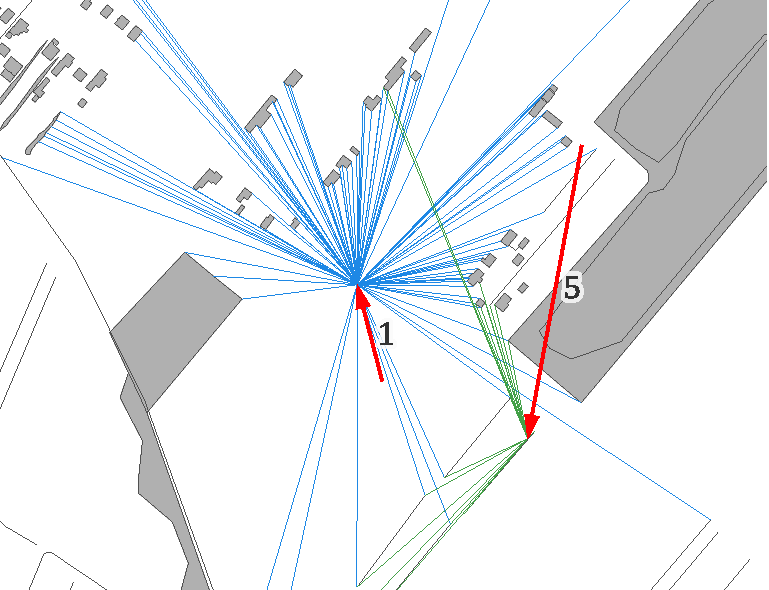
\includegraphics[width=\textwidth]{images/qgis-osm-rural}
				\end{minipage}
				\\
				\begin{minipage}[t]{0.4\textwidth}
					\captionof{table}{Measured values for the first and fifth routing requests illustrated in \Cref{fig:eval-osm-rural-map}.}
				\end{minipage}
				\hfill
				\begin{minipage}[t]{0.56\textwidth}
					\captionof{figure}{The first and fifth routing requests (red arrow between source and destination) with the nearby obstacles (gray). The bidirectional visibility edges of the two destinations are shown in blue and green.}
					\label{fig:eval-osm-rural-map}
				\end{minipage}
			\end{minipage}
		
			\todo{Times per meter?}
			
		\subsubsection{Dataset without roads or obstacles}
		
			The normal OSM-based datasets contain both, roads and obstacles.
			However, datasets containing only roads or only obstacle are thinkable and can also be used with the hybrid routing algorithm.
			For this evaluation, all roads were removed, which do not cross buildings.
			Building passages are necessary to reach backyards and were therefore kept within the dataset.
			
			\begin{figure}[h!]
				\begin{subfigure}[t]{\textwidth}
					\begin{figcenter}
						%% Creator: Matplotlib, PGF backend
%%
%% To include the figure in your LaTeX document, write
%%   \input{<filename>.pgf}
%%
%% Make sure the required packages are loaded in your preamble
%%   \usepackage{pgf}
%%
%% Also ensure that all the required font packages are loaded; for instance,
%% the lmodern package is sometimes necessary when using math font.
%%   \usepackage{lmodern}
%%
%% Figures using additional raster images can only be included by \input if
%% they are in the same directory as the main LaTeX file. For loading figures
%% from other directories you can use the `import` package
%%   \usepackage{import}
%%
%% and then include the figures with
%%   \import{<path to file>}{<filename>.pgf}
%%
%% Matplotlib used the following preamble
%%   
%%   \usepackage{fontspec}
%%   \setmainfont{DejaVuSerif.ttf}[Path=\detokenize{/home/hauke/.local/lib/python3.11/site-packages/matplotlib/mpl-data/fonts/ttf/}]
%%   \setsansfont{DroidSans.ttf}[Path=\detokenize{/usr/share/fonts/droid/}]
%%   \setmonofont{DejaVuSansMono.ttf}[Path=\detokenize{/home/hauke/.local/lib/python3.11/site-packages/matplotlib/mpl-data/fonts/ttf/}]
%%   \makeatletter\@ifpackageloaded{underscore}{}{\usepackage[strings]{underscore}}\makeatother
%%
\begingroup%
\makeatletter%
\begin{pgfpicture}%
\pgfpathrectangle{\pgfpointorigin}{\pgfqpoint{6.103826in}{1.704469in}}%
\pgfusepath{use as bounding box}%
\begin{pgfscope}%
\pgfsetbuttcap%
\pgfsetmiterjoin%
\definecolor{currentfill}{rgb}{1.000000,1.000000,1.000000}%
\pgfsetfillcolor{currentfill}%
\pgfsetlinewidth{0.000000pt}%
\definecolor{currentstroke}{rgb}{1.000000,1.000000,1.000000}%
\pgfsetstrokecolor{currentstroke}%
\pgfsetdash{}{0pt}%
\pgfpathmoveto{\pgfqpoint{0.000000in}{0.000000in}}%
\pgfpathlineto{\pgfqpoint{6.103826in}{0.000000in}}%
\pgfpathlineto{\pgfqpoint{6.103826in}{1.704469in}}%
\pgfpathlineto{\pgfqpoint{0.000000in}{1.704469in}}%
\pgfpathlineto{\pgfqpoint{0.000000in}{0.000000in}}%
\pgfpathclose%
\pgfusepath{fill}%
\end{pgfscope}%
\begin{pgfscope}%
\pgfsetbuttcap%
\pgfsetmiterjoin%
\definecolor{currentfill}{rgb}{1.000000,1.000000,1.000000}%
\pgfsetfillcolor{currentfill}%
\pgfsetlinewidth{0.000000pt}%
\definecolor{currentstroke}{rgb}{0.000000,0.000000,0.000000}%
\pgfsetstrokecolor{currentstroke}%
\pgfsetstrokeopacity{0.000000}%
\pgfsetdash{}{0pt}%
\pgfpathmoveto{\pgfqpoint{0.592976in}{0.595383in}}%
\pgfpathlineto{\pgfqpoint{4.767243in}{0.595383in}}%
\pgfpathlineto{\pgfqpoint{4.767243in}{1.704469in}}%
\pgfpathlineto{\pgfqpoint{0.592976in}{1.704469in}}%
\pgfpathlineto{\pgfqpoint{0.592976in}{0.595383in}}%
\pgfpathclose%
\pgfusepath{fill}%
\end{pgfscope}%
\begin{pgfscope}%
\definecolor{textcolor}{rgb}{0.150000,0.150000,0.150000}%
\pgfsetstrokecolor{textcolor}%
\pgfsetfillcolor{textcolor}%
\pgftext[x=0.940831in,y=0.463438in,,top]{\color{textcolor}\sffamily\fontsize{9.000000}{10.800000}\selectfont Total time}%
\end{pgfscope}%
\begin{pgfscope}%
\definecolor{textcolor}{rgb}{0.150000,0.150000,0.150000}%
\pgfsetstrokecolor{textcolor}%
\pgfsetfillcolor{textcolor}%
\pgftext[x=1.636543in,y=0.463438in,,top]{\color{textcolor}\sffamily\fontsize{9.000000}{10.800000}\selectfont kNN search}%
\end{pgfscope}%
\begin{pgfscope}%
\definecolor{textcolor}{rgb}{0.150000,0.150000,0.150000}%
\pgfsetstrokecolor{textcolor}%
\pgfsetfillcolor{textcolor}%
\pgftext[x=2.148385in, y=0.368467in, left, base]{\color{textcolor}\sffamily\fontsize{9.000000}{10.800000}\selectfont Create}%
\end{pgfscope}%
\begin{pgfscope}%
\definecolor{textcolor}{rgb}{0.150000,0.150000,0.150000}%
\pgfsetstrokecolor{textcolor}%
\pgfsetfillcolor{textcolor}%
\pgftext[x=2.168954in, y=0.224473in, left, base]{\color{textcolor}\sffamily\fontsize{9.000000}{10.800000}\selectfont graph}%
\end{pgfscope}%
\begin{pgfscope}%
\definecolor{textcolor}{rgb}{0.150000,0.150000,0.150000}%
\pgfsetstrokecolor{textcolor}%
\pgfsetfillcolor{textcolor}%
\pgftext[x=2.930217in, y=0.368467in, left, base]{\color{textcolor}\sffamily\fontsize{9.000000}{10.800000}\selectfont Get}%
\end{pgfscope}%
\begin{pgfscope}%
\definecolor{textcolor}{rgb}{0.150000,0.150000,0.150000}%
\pgfsetstrokecolor{textcolor}%
\pgfsetfillcolor{textcolor}%
\pgftext[x=2.765971in, y=0.224473in, left, base]{\color{textcolor}\sffamily\fontsize{9.000000}{10.800000}\selectfont obstacles}%
\end{pgfscope}%
\begin{pgfscope}%
\definecolor{textcolor}{rgb}{0.150000,0.150000,0.150000}%
\pgfsetstrokecolor{textcolor}%
\pgfsetfillcolor{textcolor}%
\pgftext[x=3.398664in, y=0.368467in, left, base]{\color{textcolor}\sffamily\fontsize{9.000000}{10.800000}\selectfont Merge road}%
\end{pgfscope}%
\begin{pgfscope}%
\definecolor{textcolor}{rgb}{0.150000,0.150000,0.150000}%
\pgfsetstrokecolor{textcolor}%
\pgfsetfillcolor{textcolor}%
\pgftext[x=3.559583in, y=0.224473in, left, base]{\color{textcolor}\sffamily\fontsize{9.000000}{10.800000}\selectfont edges}%
\end{pgfscope}%
\begin{pgfscope}%
\definecolor{textcolor}{rgb}{0.150000,0.150000,0.150000}%
\pgfsetstrokecolor{textcolor}%
\pgfsetfillcolor{textcolor}%
\pgftext[x=4.188949in, y=0.368467in, left, base]{\color{textcolor}\sffamily\fontsize{9.000000}{10.800000}\selectfont Add POI}%
\end{pgfscope}%
\begin{pgfscope}%
\definecolor{textcolor}{rgb}{0.150000,0.150000,0.150000}%
\pgfsetstrokecolor{textcolor}%
\pgfsetfillcolor{textcolor}%
\pgftext[x=4.145889in, y=0.224473in, left, base]{\color{textcolor}\sffamily\fontsize{9.000000}{10.800000}\selectfont attributes}%
\end{pgfscope}%
\begin{pgfscope}%
\definecolor{textcolor}{rgb}{0.150000,0.150000,0.150000}%
\pgfsetstrokecolor{textcolor}%
\pgfsetfillcolor{textcolor}%
\pgftext[x=2.680109in,y=0.125000in,,top]{\color{textcolor}\sffamily\fontsize{9.000000}{10.800000}\selectfont Input obstacle vertices}%
\end{pgfscope}%
\begin{pgfscope}%
\pgfpathrectangle{\pgfqpoint{0.592976in}{0.595383in}}{\pgfqpoint{4.174267in}{1.109087in}}%
\pgfusepath{clip}%
\pgfsetroundcap%
\pgfsetroundjoin%
\pgfsetlinewidth{1.003750pt}%
\definecolor{currentstroke}{rgb}{0.800000,0.800000,0.800000}%
\pgfsetstrokecolor{currentstroke}%
\pgfsetdash{}{0pt}%
\pgfpathmoveto{\pgfqpoint{0.592976in}{0.891511in}}%
\pgfpathlineto{\pgfqpoint{4.767243in}{0.891511in}}%
\pgfusepath{stroke}%
\end{pgfscope}%
\begin{pgfscope}%
\definecolor{textcolor}{rgb}{0.150000,0.150000,0.150000}%
\pgfsetstrokecolor{textcolor}%
\pgfsetfillcolor{textcolor}%
\pgftext[x=0.194444in, y=0.844025in, left, base]{\color{textcolor}\sffamily\fontsize{9.000000}{10.800000}\selectfont \(\displaystyle {10^{-3}}\)}%
\end{pgfscope}%
\begin{pgfscope}%
\pgfpathrectangle{\pgfqpoint{0.592976in}{0.595383in}}{\pgfqpoint{4.174267in}{1.109087in}}%
\pgfusepath{clip}%
\pgfsetroundcap%
\pgfsetroundjoin%
\pgfsetlinewidth{1.003750pt}%
\definecolor{currentstroke}{rgb}{0.800000,0.800000,0.800000}%
\pgfsetstrokecolor{currentstroke}%
\pgfsetdash{}{0pt}%
\pgfpathmoveto{\pgfqpoint{0.592976in}{1.273824in}}%
\pgfpathlineto{\pgfqpoint{4.767243in}{1.273824in}}%
\pgfusepath{stroke}%
\end{pgfscope}%
\begin{pgfscope}%
\definecolor{textcolor}{rgb}{0.150000,0.150000,0.150000}%
\pgfsetstrokecolor{textcolor}%
\pgfsetfillcolor{textcolor}%
\pgftext[x=0.274690in, y=1.226339in, left, base]{\color{textcolor}\sffamily\fontsize{9.000000}{10.800000}\selectfont \(\displaystyle {10^{0}}\)}%
\end{pgfscope}%
\begin{pgfscope}%
\pgfpathrectangle{\pgfqpoint{0.592976in}{0.595383in}}{\pgfqpoint{4.174267in}{1.109087in}}%
\pgfusepath{clip}%
\pgfsetroundcap%
\pgfsetroundjoin%
\pgfsetlinewidth{1.003750pt}%
\definecolor{currentstroke}{rgb}{0.800000,0.800000,0.800000}%
\pgfsetstrokecolor{currentstroke}%
\pgfsetdash{}{0pt}%
\pgfpathmoveto{\pgfqpoint{0.592976in}{1.656137in}}%
\pgfpathlineto{\pgfqpoint{4.767243in}{1.656137in}}%
\pgfusepath{stroke}%
\end{pgfscope}%
\begin{pgfscope}%
\definecolor{textcolor}{rgb}{0.150000,0.150000,0.150000}%
\pgfsetstrokecolor{textcolor}%
\pgfsetfillcolor{textcolor}%
\pgftext[x=0.274690in, y=1.608652in, left, base]{\color{textcolor}\sffamily\fontsize{9.000000}{10.800000}\selectfont \(\displaystyle {10^{3}}\)}%
\end{pgfscope}%
\begin{pgfscope}%
\definecolor{textcolor}{rgb}{0.150000,0.150000,0.150000}%
\pgfsetstrokecolor{textcolor}%
\pgfsetfillcolor{textcolor}%
\pgftext[x=0.125000in,y=1.149926in,,bottom,rotate=90.000000]{\color{textcolor}\sffamily\fontsize{9.000000}{10.800000}\selectfont Time in s}%
\end{pgfscope}%
\begin{pgfscope}%
\pgfpathrectangle{\pgfqpoint{0.592976in}{0.595383in}}{\pgfqpoint{4.174267in}{1.109087in}}%
\pgfusepath{clip}%
\pgfsetbuttcap%
\pgfsetmiterjoin%
\definecolor{currentfill}{rgb}{0.349020,0.490196,0.749020}%
\pgfsetfillcolor{currentfill}%
\pgfsetlinewidth{1.003750pt}%
\definecolor{currentstroke}{rgb}{1.000000,1.000000,1.000000}%
\pgfsetstrokecolor{currentstroke}%
\pgfsetdash{}{0pt}%
\pgfpathmoveto{\pgfqpoint{0.662547in}{-126.163917in}}%
\pgfpathlineto{\pgfqpoint{0.848070in}{-126.163917in}}%
\pgfpathlineto{\pgfqpoint{0.848070in}{1.654056in}}%
\pgfpathlineto{\pgfqpoint{0.662547in}{1.654056in}}%
\pgfpathlineto{\pgfqpoint{0.662547in}{-126.163917in}}%
\pgfpathclose%
\pgfusepath{stroke,fill}%
\end{pgfscope}%
\begin{pgfscope}%
\pgfpathrectangle{\pgfqpoint{0.592976in}{0.595383in}}{\pgfqpoint{4.174267in}{1.109087in}}%
\pgfusepath{clip}%
\pgfsetbuttcap%
\pgfsetmiterjoin%
\definecolor{currentfill}{rgb}{0.349020,0.490196,0.749020}%
\pgfsetfillcolor{currentfill}%
\pgfsetlinewidth{1.003750pt}%
\definecolor{currentstroke}{rgb}{1.000000,1.000000,1.000000}%
\pgfsetstrokecolor{currentstroke}%
\pgfsetdash{}{0pt}%
\pgfpathmoveto{\pgfqpoint{1.358258in}{-126.163917in}}%
\pgfpathlineto{\pgfqpoint{1.543781in}{-126.163917in}}%
\pgfpathlineto{\pgfqpoint{1.543781in}{1.621794in}}%
\pgfpathlineto{\pgfqpoint{1.358258in}{1.621794in}}%
\pgfpathlineto{\pgfqpoint{1.358258in}{-126.163917in}}%
\pgfpathclose%
\pgfusepath{stroke,fill}%
\end{pgfscope}%
\begin{pgfscope}%
\pgfpathrectangle{\pgfqpoint{0.592976in}{0.595383in}}{\pgfqpoint{4.174267in}{1.109087in}}%
\pgfusepath{clip}%
\pgfsetbuttcap%
\pgfsetmiterjoin%
\definecolor{currentfill}{rgb}{0.349020,0.490196,0.749020}%
\pgfsetfillcolor{currentfill}%
\pgfsetlinewidth{1.003750pt}%
\definecolor{currentstroke}{rgb}{1.000000,1.000000,1.000000}%
\pgfsetstrokecolor{currentstroke}%
\pgfsetdash{}{0pt}%
\pgfpathmoveto{\pgfqpoint{2.053969in}{-126.163917in}}%
\pgfpathlineto{\pgfqpoint{2.239492in}{-126.163917in}}%
\pgfpathlineto{\pgfqpoint{2.239492in}{1.282485in}}%
\pgfpathlineto{\pgfqpoint{2.053969in}{1.282485in}}%
\pgfpathlineto{\pgfqpoint{2.053969in}{-126.163917in}}%
\pgfpathclose%
\pgfusepath{stroke,fill}%
\end{pgfscope}%
\begin{pgfscope}%
\pgfpathrectangle{\pgfqpoint{0.592976in}{0.595383in}}{\pgfqpoint{4.174267in}{1.109087in}}%
\pgfusepath{clip}%
\pgfsetbuttcap%
\pgfsetmiterjoin%
\definecolor{currentfill}{rgb}{0.349020,0.490196,0.749020}%
\pgfsetfillcolor{currentfill}%
\pgfsetlinewidth{1.003750pt}%
\definecolor{currentstroke}{rgb}{1.000000,1.000000,1.000000}%
\pgfsetstrokecolor{currentstroke}%
\pgfsetdash{}{0pt}%
\pgfpathmoveto{\pgfqpoint{2.749680in}{-126.163917in}}%
\pgfpathlineto{\pgfqpoint{2.935203in}{-126.163917in}}%
\pgfpathlineto{\pgfqpoint{2.935203in}{1.184746in}}%
\pgfpathlineto{\pgfqpoint{2.749680in}{1.184746in}}%
\pgfpathlineto{\pgfqpoint{2.749680in}{-126.163917in}}%
\pgfpathclose%
\pgfusepath{stroke,fill}%
\end{pgfscope}%
\begin{pgfscope}%
\pgfpathrectangle{\pgfqpoint{0.592976in}{0.595383in}}{\pgfqpoint{4.174267in}{1.109087in}}%
\pgfusepath{clip}%
\pgfsetbuttcap%
\pgfsetmiterjoin%
\definecolor{currentfill}{rgb}{0.349020,0.490196,0.749020}%
\pgfsetfillcolor{currentfill}%
\pgfsetlinewidth{1.003750pt}%
\definecolor{currentstroke}{rgb}{1.000000,1.000000,1.000000}%
\pgfsetstrokecolor{currentstroke}%
\pgfsetdash{}{0pt}%
\pgfpathmoveto{\pgfqpoint{3.445391in}{-126.163917in}}%
\pgfpathlineto{\pgfqpoint{3.630914in}{-126.163917in}}%
\pgfpathlineto{\pgfqpoint{3.630914in}{1.608561in}}%
\pgfpathlineto{\pgfqpoint{3.445391in}{1.608561in}}%
\pgfpathlineto{\pgfqpoint{3.445391in}{-126.163917in}}%
\pgfpathclose%
\pgfusepath{stroke,fill}%
\end{pgfscope}%
\begin{pgfscope}%
\pgfpathrectangle{\pgfqpoint{0.592976in}{0.595383in}}{\pgfqpoint{4.174267in}{1.109087in}}%
\pgfusepath{clip}%
\pgfsetbuttcap%
\pgfsetmiterjoin%
\definecolor{currentfill}{rgb}{0.349020,0.490196,0.749020}%
\pgfsetfillcolor{currentfill}%
\pgfsetlinewidth{1.003750pt}%
\definecolor{currentstroke}{rgb}{1.000000,1.000000,1.000000}%
\pgfsetstrokecolor{currentstroke}%
\pgfsetdash{}{0pt}%
\pgfpathmoveto{\pgfqpoint{4.141103in}{-126.163917in}}%
\pgfpathlineto{\pgfqpoint{4.326626in}{-126.163917in}}%
\pgfpathlineto{\pgfqpoint{4.326626in}{1.116913in}}%
\pgfpathlineto{\pgfqpoint{4.141103in}{1.116913in}}%
\pgfpathlineto{\pgfqpoint{4.141103in}{-126.163917in}}%
\pgfpathclose%
\pgfusepath{stroke,fill}%
\end{pgfscope}%
\begin{pgfscope}%
\pgfpathrectangle{\pgfqpoint{0.592976in}{0.595383in}}{\pgfqpoint{4.174267in}{1.109087in}}%
\pgfusepath{clip}%
\pgfsetbuttcap%
\pgfsetmiterjoin%
\definecolor{currentfill}{rgb}{0.852941,0.544118,0.370588}%
\pgfsetfillcolor{currentfill}%
\pgfsetlinewidth{1.003750pt}%
\definecolor{currentstroke}{rgb}{1.000000,1.000000,1.000000}%
\pgfsetstrokecolor{currentstroke}%
\pgfsetdash{}{0pt}%
\pgfpathmoveto{\pgfqpoint{0.848070in}{-126.163917in}}%
\pgfpathlineto{\pgfqpoint{1.033593in}{-126.163917in}}%
\pgfpathlineto{\pgfqpoint{1.033593in}{1.621550in}}%
\pgfpathlineto{\pgfqpoint{0.848070in}{1.621550in}}%
\pgfpathlineto{\pgfqpoint{0.848070in}{-126.163917in}}%
\pgfpathclose%
\pgfusepath{stroke,fill}%
\end{pgfscope}%
\begin{pgfscope}%
\pgfpathrectangle{\pgfqpoint{0.592976in}{0.595383in}}{\pgfqpoint{4.174267in}{1.109087in}}%
\pgfusepath{clip}%
\pgfsetbuttcap%
\pgfsetmiterjoin%
\definecolor{currentfill}{rgb}{0.852941,0.544118,0.370588}%
\pgfsetfillcolor{currentfill}%
\pgfsetlinewidth{1.003750pt}%
\definecolor{currentstroke}{rgb}{1.000000,1.000000,1.000000}%
\pgfsetstrokecolor{currentstroke}%
\pgfsetdash{}{0pt}%
\pgfpathmoveto{\pgfqpoint{1.543781in}{-126.163917in}}%
\pgfpathlineto{\pgfqpoint{1.729304in}{-126.163917in}}%
\pgfpathlineto{\pgfqpoint{1.729304in}{1.619104in}}%
\pgfpathlineto{\pgfqpoint{1.543781in}{1.619104in}}%
\pgfpathlineto{\pgfqpoint{1.543781in}{-126.163917in}}%
\pgfpathclose%
\pgfusepath{stroke,fill}%
\end{pgfscope}%
\begin{pgfscope}%
\pgfpathrectangle{\pgfqpoint{0.592976in}{0.595383in}}{\pgfqpoint{4.174267in}{1.109087in}}%
\pgfusepath{clip}%
\pgfsetbuttcap%
\pgfsetmiterjoin%
\definecolor{currentfill}{rgb}{0.852941,0.544118,0.370588}%
\pgfsetfillcolor{currentfill}%
\pgfsetlinewidth{1.003750pt}%
\definecolor{currentstroke}{rgb}{1.000000,1.000000,1.000000}%
\pgfsetstrokecolor{currentstroke}%
\pgfsetdash{}{0pt}%
\pgfpathmoveto{\pgfqpoint{2.239492in}{-126.163917in}}%
\pgfpathlineto{\pgfqpoint{2.425015in}{-126.163917in}}%
\pgfpathlineto{\pgfqpoint{2.425015in}{1.276251in}}%
\pgfpathlineto{\pgfqpoint{2.239492in}{1.276251in}}%
\pgfpathlineto{\pgfqpoint{2.239492in}{-126.163917in}}%
\pgfpathclose%
\pgfusepath{stroke,fill}%
\end{pgfscope}%
\begin{pgfscope}%
\pgfpathrectangle{\pgfqpoint{0.592976in}{0.595383in}}{\pgfqpoint{4.174267in}{1.109087in}}%
\pgfusepath{clip}%
\pgfsetbuttcap%
\pgfsetmiterjoin%
\definecolor{currentfill}{rgb}{0.852941,0.544118,0.370588}%
\pgfsetfillcolor{currentfill}%
\pgfsetlinewidth{1.003750pt}%
\definecolor{currentstroke}{rgb}{1.000000,1.000000,1.000000}%
\pgfsetstrokecolor{currentstroke}%
\pgfsetdash{}{0pt}%
\pgfpathmoveto{\pgfqpoint{2.935203in}{-126.163917in}}%
\pgfpathlineto{\pgfqpoint{3.120726in}{-126.163917in}}%
\pgfpathlineto{\pgfqpoint{3.120726in}{1.185267in}}%
\pgfpathlineto{\pgfqpoint{2.935203in}{1.185267in}}%
\pgfpathlineto{\pgfqpoint{2.935203in}{-126.163917in}}%
\pgfpathclose%
\pgfusepath{stroke,fill}%
\end{pgfscope}%
\begin{pgfscope}%
\pgfpathrectangle{\pgfqpoint{0.592976in}{0.595383in}}{\pgfqpoint{4.174267in}{1.109087in}}%
\pgfusepath{clip}%
\pgfsetbuttcap%
\pgfsetmiterjoin%
\definecolor{currentfill}{rgb}{0.852941,0.544118,0.370588}%
\pgfsetfillcolor{currentfill}%
\pgfsetlinewidth{1.003750pt}%
\definecolor{currentstroke}{rgb}{1.000000,1.000000,1.000000}%
\pgfsetstrokecolor{currentstroke}%
\pgfsetdash{}{0pt}%
\pgfpathmoveto{\pgfqpoint{3.630914in}{-126.163917in}}%
\pgfpathlineto{\pgfqpoint{3.816437in}{-126.163917in}}%
\pgfpathlineto{\pgfqpoint{3.816437in}{1.444306in}}%
\pgfpathlineto{\pgfqpoint{3.630914in}{1.444306in}}%
\pgfpathlineto{\pgfqpoint{3.630914in}{-126.163917in}}%
\pgfpathclose%
\pgfusepath{stroke,fill}%
\end{pgfscope}%
\begin{pgfscope}%
\pgfpathrectangle{\pgfqpoint{0.592976in}{0.595383in}}{\pgfqpoint{4.174267in}{1.109087in}}%
\pgfusepath{clip}%
\pgfsetbuttcap%
\pgfsetmiterjoin%
\definecolor{currentfill}{rgb}{0.852941,0.544118,0.370588}%
\pgfsetfillcolor{currentfill}%
\pgfsetlinewidth{1.003750pt}%
\definecolor{currentstroke}{rgb}{1.000000,1.000000,1.000000}%
\pgfsetstrokecolor{currentstroke}%
\pgfsetdash{}{0pt}%
\pgfpathmoveto{\pgfqpoint{4.326626in}{-126.163917in}}%
\pgfpathlineto{\pgfqpoint{4.512149in}{-126.163917in}}%
\pgfpathlineto{\pgfqpoint{4.512149in}{1.084764in}}%
\pgfpathlineto{\pgfqpoint{4.326626in}{1.084764in}}%
\pgfpathlineto{\pgfqpoint{4.326626in}{-126.163917in}}%
\pgfpathclose%
\pgfusepath{stroke,fill}%
\end{pgfscope}%
\begin{pgfscope}%
\pgfpathrectangle{\pgfqpoint{0.592976in}{0.595383in}}{\pgfqpoint{4.174267in}{1.109087in}}%
\pgfusepath{clip}%
\pgfsetbuttcap%
\pgfsetmiterjoin%
\definecolor{currentfill}{rgb}{0.460784,0.749020,0.443137}%
\pgfsetfillcolor{currentfill}%
\pgfsetlinewidth{1.003750pt}%
\definecolor{currentstroke}{rgb}{1.000000,1.000000,1.000000}%
\pgfsetstrokecolor{currentstroke}%
\pgfsetdash{}{0pt}%
\pgfpathmoveto{\pgfqpoint{1.033593in}{-126.163917in}}%
\pgfpathlineto{\pgfqpoint{1.219116in}{-126.163917in}}%
\pgfpathlineto{\pgfqpoint{1.219116in}{1.293809in}}%
\pgfpathlineto{\pgfqpoint{1.033593in}{1.293809in}}%
\pgfpathlineto{\pgfqpoint{1.033593in}{-126.163917in}}%
\pgfpathclose%
\pgfusepath{stroke,fill}%
\end{pgfscope}%
\begin{pgfscope}%
\pgfpathrectangle{\pgfqpoint{0.592976in}{0.595383in}}{\pgfqpoint{4.174267in}{1.109087in}}%
\pgfusepath{clip}%
\pgfsetbuttcap%
\pgfsetmiterjoin%
\definecolor{currentfill}{rgb}{0.460784,0.749020,0.443137}%
\pgfsetfillcolor{currentfill}%
\pgfsetlinewidth{1.003750pt}%
\definecolor{currentstroke}{rgb}{1.000000,1.000000,1.000000}%
\pgfsetstrokecolor{currentstroke}%
\pgfsetdash{}{0pt}%
\pgfpathmoveto{\pgfqpoint{1.729304in}{-126.163917in}}%
\pgfpathlineto{\pgfqpoint{1.914827in}{-126.163917in}}%
\pgfpathlineto{\pgfqpoint{1.914827in}{0.645796in}}%
\pgfpathlineto{\pgfqpoint{1.729304in}{0.645796in}}%
\pgfpathlineto{\pgfqpoint{1.729304in}{-126.163917in}}%
\pgfpathclose%
\pgfusepath{stroke,fill}%
\end{pgfscope}%
\begin{pgfscope}%
\pgfpathrectangle{\pgfqpoint{0.592976in}{0.595383in}}{\pgfqpoint{4.174267in}{1.109087in}}%
\pgfusepath{clip}%
\pgfsetbuttcap%
\pgfsetmiterjoin%
\definecolor{currentfill}{rgb}{0.460784,0.749020,0.443137}%
\pgfsetfillcolor{currentfill}%
\pgfsetlinewidth{1.003750pt}%
\definecolor{currentstroke}{rgb}{1.000000,1.000000,1.000000}%
\pgfsetstrokecolor{currentstroke}%
\pgfsetdash{}{0pt}%
\pgfpathmoveto{\pgfqpoint{2.425015in}{-126.163917in}}%
\pgfpathlineto{\pgfqpoint{2.610538in}{-126.163917in}}%
\pgfpathlineto{\pgfqpoint{2.610538in}{0.652833in}}%
\pgfpathlineto{\pgfqpoint{2.425015in}{0.652833in}}%
\pgfpathlineto{\pgfqpoint{2.425015in}{-126.163917in}}%
\pgfpathclose%
\pgfusepath{stroke,fill}%
\end{pgfscope}%
\begin{pgfscope}%
\pgfpathrectangle{\pgfqpoint{0.592976in}{0.595383in}}{\pgfqpoint{4.174267in}{1.109087in}}%
\pgfusepath{clip}%
\pgfsetbuttcap%
\pgfsetmiterjoin%
\definecolor{currentfill}{rgb}{0.460784,0.749020,0.443137}%
\pgfsetfillcolor{currentfill}%
\pgfsetlinewidth{1.003750pt}%
\definecolor{currentstroke}{rgb}{1.000000,1.000000,1.000000}%
\pgfsetstrokecolor{currentstroke}%
\pgfsetdash{}{0pt}%
\pgfpathmoveto{\pgfqpoint{3.120726in}{-126.163917in}}%
\pgfpathlineto{\pgfqpoint{3.306249in}{-126.163917in}}%
\pgfpathlineto{\pgfqpoint{3.306249in}{1.020032in}}%
\pgfpathlineto{\pgfqpoint{3.120726in}{1.020032in}}%
\pgfpathlineto{\pgfqpoint{3.120726in}{-126.163917in}}%
\pgfpathclose%
\pgfusepath{stroke,fill}%
\end{pgfscope}%
\begin{pgfscope}%
\pgfpathrectangle{\pgfqpoint{0.592976in}{0.595383in}}{\pgfqpoint{4.174267in}{1.109087in}}%
\pgfusepath{clip}%
\pgfsetbuttcap%
\pgfsetmiterjoin%
\definecolor{currentfill}{rgb}{0.460784,0.749020,0.443137}%
\pgfsetfillcolor{currentfill}%
\pgfsetlinewidth{1.003750pt}%
\definecolor{currentstroke}{rgb}{1.000000,1.000000,1.000000}%
\pgfsetstrokecolor{currentstroke}%
\pgfsetdash{}{0pt}%
\pgfpathmoveto{\pgfqpoint{3.816437in}{-126.163917in}}%
\pgfpathlineto{\pgfqpoint{4.001960in}{-126.163917in}}%
\pgfpathlineto{\pgfqpoint{4.001960in}{1.291903in}}%
\pgfpathlineto{\pgfqpoint{3.816437in}{1.291903in}}%
\pgfpathlineto{\pgfqpoint{3.816437in}{-126.163917in}}%
\pgfpathclose%
\pgfusepath{stroke,fill}%
\end{pgfscope}%
\begin{pgfscope}%
\pgfpathrectangle{\pgfqpoint{0.592976in}{0.595383in}}{\pgfqpoint{4.174267in}{1.109087in}}%
\pgfusepath{clip}%
\pgfsetbuttcap%
\pgfsetmiterjoin%
\definecolor{currentfill}{rgb}{0.460784,0.749020,0.443137}%
\pgfsetfillcolor{currentfill}%
\pgfsetlinewidth{1.003750pt}%
\definecolor{currentstroke}{rgb}{1.000000,1.000000,1.000000}%
\pgfsetstrokecolor{currentstroke}%
\pgfsetdash{}{0pt}%
\pgfpathmoveto{\pgfqpoint{4.512149in}{-126.163917in}}%
\pgfpathlineto{\pgfqpoint{4.697672in}{-126.163917in}}%
\pgfpathlineto{\pgfqpoint{4.697672in}{1.028773in}}%
\pgfpathlineto{\pgfqpoint{4.512149in}{1.028773in}}%
\pgfpathlineto{\pgfqpoint{4.512149in}{-126.163917in}}%
\pgfpathclose%
\pgfusepath{stroke,fill}%
\end{pgfscope}%
\begin{pgfscope}%
\pgfsetrectcap%
\pgfsetmiterjoin%
\pgfsetlinewidth{1.254687pt}%
\definecolor{currentstroke}{rgb}{0.800000,0.800000,0.800000}%
\pgfsetstrokecolor{currentstroke}%
\pgfsetdash{}{0pt}%
\pgfpathmoveto{\pgfqpoint{0.592976in}{0.595383in}}%
\pgfpathlineto{\pgfqpoint{0.592976in}{1.704469in}}%
\pgfusepath{stroke}%
\end{pgfscope}%
\begin{pgfscope}%
\pgfsetrectcap%
\pgfsetmiterjoin%
\pgfsetlinewidth{1.254687pt}%
\definecolor{currentstroke}{rgb}{0.800000,0.800000,0.800000}%
\pgfsetstrokecolor{currentstroke}%
\pgfsetdash{}{0pt}%
\pgfpathmoveto{\pgfqpoint{4.767243in}{0.595383in}}%
\pgfpathlineto{\pgfqpoint{4.767243in}{1.704469in}}%
\pgfusepath{stroke}%
\end{pgfscope}%
\begin{pgfscope}%
\pgfsetrectcap%
\pgfsetmiterjoin%
\pgfsetlinewidth{1.254687pt}%
\definecolor{currentstroke}{rgb}{0.800000,0.800000,0.800000}%
\pgfsetstrokecolor{currentstroke}%
\pgfsetdash{}{0pt}%
\pgfpathmoveto{\pgfqpoint{0.592976in}{0.595383in}}%
\pgfpathlineto{\pgfqpoint{4.767243in}{0.595383in}}%
\pgfusepath{stroke}%
\end{pgfscope}%
\begin{pgfscope}%
\pgfsetrectcap%
\pgfsetmiterjoin%
\pgfsetlinewidth{1.254687pt}%
\definecolor{currentstroke}{rgb}{0.800000,0.800000,0.800000}%
\pgfsetstrokecolor{currentstroke}%
\pgfsetdash{}{0pt}%
\pgfpathmoveto{\pgfqpoint{0.592976in}{1.704469in}}%
\pgfpathlineto{\pgfqpoint{4.767243in}{1.704469in}}%
\pgfusepath{stroke}%
\end{pgfscope}%
\begin{pgfscope}%
\pgfsetbuttcap%
\pgfsetmiterjoin%
\definecolor{currentfill}{rgb}{1.000000,1.000000,1.000000}%
\pgfsetfillcolor{currentfill}%
\pgfsetfillopacity{0.800000}%
\pgfsetlinewidth{1.003750pt}%
\definecolor{currentstroke}{rgb}{0.800000,0.800000,0.800000}%
\pgfsetstrokecolor{currentstroke}%
\pgfsetstrokeopacity{0.800000}%
\pgfsetdash{}{0pt}%
\pgfpathmoveto{\pgfqpoint{4.959099in}{0.756176in}}%
\pgfpathlineto{\pgfqpoint{6.078826in}{0.756176in}}%
\pgfpathquadraticcurveto{\pgfqpoint{6.103826in}{0.756176in}}{\pgfqpoint{6.103826in}{0.781176in}}%
\pgfpathlineto{\pgfqpoint{6.103826in}{1.518676in}}%
\pgfpathquadraticcurveto{\pgfqpoint{6.103826in}{1.543676in}}{\pgfqpoint{6.078826in}{1.543676in}}%
\pgfpathlineto{\pgfqpoint{4.959099in}{1.543676in}}%
\pgfpathquadraticcurveto{\pgfqpoint{4.934099in}{1.543676in}}{\pgfqpoint{4.934099in}{1.518676in}}%
\pgfpathlineto{\pgfqpoint{4.934099in}{0.781176in}}%
\pgfpathquadraticcurveto{\pgfqpoint{4.934099in}{0.756176in}}{\pgfqpoint{4.959099in}{0.756176in}}%
\pgfpathlineto{\pgfqpoint{4.959099in}{0.756176in}}%
\pgfpathclose%
\pgfusepath{stroke,fill}%
\end{pgfscope}%
\begin{pgfscope}%
\definecolor{textcolor}{rgb}{0.150000,0.150000,0.150000}%
\pgfsetstrokecolor{textcolor}%
\pgfsetfillcolor{textcolor}%
\pgftext[x=5.305858in,y=1.398705in,left,base]{\color{textcolor}\sffamily\fontsize{9.000000}{10.800000}\selectfont Dataset}%
\end{pgfscope}%
\begin{pgfscope}%
\pgfsetbuttcap%
\pgfsetmiterjoin%
\definecolor{currentfill}{rgb}{0.349020,0.490196,0.749020}%
\pgfsetfillcolor{currentfill}%
\pgfsetlinewidth{1.003750pt}%
\definecolor{currentstroke}{rgb}{1.000000,1.000000,1.000000}%
\pgfsetstrokecolor{currentstroke}%
\pgfsetdash{}{0pt}%
\pgfpathmoveto{\pgfqpoint{4.984099in}{1.211205in}}%
\pgfpathlineto{\pgfqpoint{5.234099in}{1.211205in}}%
\pgfpathlineto{\pgfqpoint{5.234099in}{1.298705in}}%
\pgfpathlineto{\pgfqpoint{4.984099in}{1.298705in}}%
\pgfpathlineto{\pgfqpoint{4.984099in}{1.211205in}}%
\pgfpathclose%
\pgfusepath{stroke,fill}%
\end{pgfscope}%
\begin{pgfscope}%
\definecolor{textcolor}{rgb}{0.150000,0.150000,0.150000}%
\pgfsetstrokecolor{textcolor}%
\pgfsetfillcolor{textcolor}%
\pgftext[x=5.334099in,y=1.211205in,left,base]{\color{textcolor}\sffamily\fontsize{9.000000}{10.800000}\selectfont Normal}%
\end{pgfscope}%
\begin{pgfscope}%
\pgfsetbuttcap%
\pgfsetmiterjoin%
\definecolor{currentfill}{rgb}{0.852941,0.544118,0.370588}%
\pgfsetfillcolor{currentfill}%
\pgfsetlinewidth{1.003750pt}%
\definecolor{currentstroke}{rgb}{1.000000,1.000000,1.000000}%
\pgfsetstrokecolor{currentstroke}%
\pgfsetdash{}{0pt}%
\pgfpathmoveto{\pgfqpoint{4.984099in}{1.023705in}}%
\pgfpathlineto{\pgfqpoint{5.234099in}{1.023705in}}%
\pgfpathlineto{\pgfqpoint{5.234099in}{1.111205in}}%
\pgfpathlineto{\pgfqpoint{4.984099in}{1.111205in}}%
\pgfpathlineto{\pgfqpoint{4.984099in}{1.023705in}}%
\pgfpathclose%
\pgfusepath{stroke,fill}%
\end{pgfscope}%
\begin{pgfscope}%
\definecolor{textcolor}{rgb}{0.150000,0.150000,0.150000}%
\pgfsetstrokecolor{textcolor}%
\pgfsetfillcolor{textcolor}%
\pgftext[x=5.334099in,y=1.023705in,left,base]{\color{textcolor}\sffamily\fontsize{9.000000}{10.800000}\selectfont No roads}%
\end{pgfscope}%
\begin{pgfscope}%
\pgfsetbuttcap%
\pgfsetmiterjoin%
\definecolor{currentfill}{rgb}{0.460784,0.749020,0.443137}%
\pgfsetfillcolor{currentfill}%
\pgfsetlinewidth{1.003750pt}%
\definecolor{currentstroke}{rgb}{1.000000,1.000000,1.000000}%
\pgfsetstrokecolor{currentstroke}%
\pgfsetdash{}{0pt}%
\pgfpathmoveto{\pgfqpoint{4.984099in}{0.836205in}}%
\pgfpathlineto{\pgfqpoint{5.234099in}{0.836205in}}%
\pgfpathlineto{\pgfqpoint{5.234099in}{0.923705in}}%
\pgfpathlineto{\pgfqpoint{4.984099in}{0.923705in}}%
\pgfpathlineto{\pgfqpoint{4.984099in}{0.836205in}}%
\pgfpathclose%
\pgfusepath{stroke,fill}%
\end{pgfscope}%
\begin{pgfscope}%
\definecolor{textcolor}{rgb}{0.150000,0.150000,0.150000}%
\pgfsetstrokecolor{textcolor}%
\pgfsetfillcolor{textcolor}%
\pgftext[x=5.334099in,y=0.836205in,left,base]{\color{textcolor}\sffamily\fontsize{9.000000}{10.800000}\selectfont No obstacles}%
\end{pgfscope}%
\end{pgfpicture}%
\makeatother%
\endgroup%

					\end{figcenter}
					\caption{\enquote{OSM city} dataset.}
					\label{fig:eval-import-osm-no-roads-obstacles-city}
				\end{subfigure}
				\\[3ex]
				\begin{subfigure}[t]{\textwidth}
					\begin{figcenter}
						%% Creator: Matplotlib, PGF backend
%%
%% To include the figure in your LaTeX document, write
%%   \input{<filename>.pgf}
%%
%% Make sure the required packages are loaded in your preamble
%%   \usepackage{pgf}
%%
%% Also ensure that all the required font packages are loaded; for instance,
%% the lmodern package is sometimes necessary when using math font.
%%   \usepackage{lmodern}
%%
%% Figures using additional raster images can only be included by \input if
%% they are in the same directory as the main LaTeX file. For loading figures
%% from other directories you can use the `import` package
%%   \usepackage{import}
%%
%% and then include the figures with
%%   \import{<path to file>}{<filename>.pgf}
%%
%% Matplotlib used the following preamble
%%   
%%   \usepackage{fontspec}
%%   \setmainfont{DejaVuSerif.ttf}[Path=\detokenize{/home/hauke/.local/lib/python3.11/site-packages/matplotlib/mpl-data/fonts/ttf/}]
%%   \setsansfont{DroidSans.ttf}[Path=\detokenize{/usr/share/fonts/droid/}]
%%   \setmonofont{DejaVuSansMono.ttf}[Path=\detokenize{/home/hauke/.local/lib/python3.11/site-packages/matplotlib/mpl-data/fonts/ttf/}]
%%   \makeatletter\@ifpackageloaded{underscore}{}{\usepackage[strings]{underscore}}\makeatother
%%
\begingroup%
\makeatletter%
\begin{pgfpicture}%
\pgfpathrectangle{\pgfpointorigin}{\pgfqpoint{6.103826in}{1.704469in}}%
\pgfusepath{use as bounding box}%
\begin{pgfscope}%
\pgfsetbuttcap%
\pgfsetmiterjoin%
\definecolor{currentfill}{rgb}{1.000000,1.000000,1.000000}%
\pgfsetfillcolor{currentfill}%
\pgfsetlinewidth{0.000000pt}%
\definecolor{currentstroke}{rgb}{1.000000,1.000000,1.000000}%
\pgfsetstrokecolor{currentstroke}%
\pgfsetdash{}{0pt}%
\pgfpathmoveto{\pgfqpoint{0.000000in}{0.000000in}}%
\pgfpathlineto{\pgfqpoint{6.103826in}{0.000000in}}%
\pgfpathlineto{\pgfqpoint{6.103826in}{1.704469in}}%
\pgfpathlineto{\pgfqpoint{0.000000in}{1.704469in}}%
\pgfpathlineto{\pgfqpoint{0.000000in}{0.000000in}}%
\pgfpathclose%
\pgfusepath{fill}%
\end{pgfscope}%
\begin{pgfscope}%
\pgfsetbuttcap%
\pgfsetmiterjoin%
\definecolor{currentfill}{rgb}{1.000000,1.000000,1.000000}%
\pgfsetfillcolor{currentfill}%
\pgfsetlinewidth{0.000000pt}%
\definecolor{currentstroke}{rgb}{0.000000,0.000000,0.000000}%
\pgfsetstrokecolor{currentstroke}%
\pgfsetstrokeopacity{0.000000}%
\pgfsetdash{}{0pt}%
\pgfpathmoveto{\pgfqpoint{0.592976in}{0.595383in}}%
\pgfpathlineto{\pgfqpoint{4.767243in}{0.595383in}}%
\pgfpathlineto{\pgfqpoint{4.767243in}{1.704469in}}%
\pgfpathlineto{\pgfqpoint{0.592976in}{1.704469in}}%
\pgfpathlineto{\pgfqpoint{0.592976in}{0.595383in}}%
\pgfpathclose%
\pgfusepath{fill}%
\end{pgfscope}%
\begin{pgfscope}%
\definecolor{textcolor}{rgb}{0.150000,0.150000,0.150000}%
\pgfsetstrokecolor{textcolor}%
\pgfsetfillcolor{textcolor}%
\pgftext[x=0.940831in,y=0.463438in,,top]{\color{textcolor}\sffamily\fontsize{9.000000}{10.800000}\selectfont Total time}%
\end{pgfscope}%
\begin{pgfscope}%
\definecolor{textcolor}{rgb}{0.150000,0.150000,0.150000}%
\pgfsetstrokecolor{textcolor}%
\pgfsetfillcolor{textcolor}%
\pgftext[x=1.636543in,y=0.463438in,,top]{\color{textcolor}\sffamily\fontsize{9.000000}{10.800000}\selectfont kNN search}%
\end{pgfscope}%
\begin{pgfscope}%
\definecolor{textcolor}{rgb}{0.150000,0.150000,0.150000}%
\pgfsetstrokecolor{textcolor}%
\pgfsetfillcolor{textcolor}%
\pgftext[x=2.148385in, y=0.368467in, left, base]{\color{textcolor}\sffamily\fontsize{9.000000}{10.800000}\selectfont Create}%
\end{pgfscope}%
\begin{pgfscope}%
\definecolor{textcolor}{rgb}{0.150000,0.150000,0.150000}%
\pgfsetstrokecolor{textcolor}%
\pgfsetfillcolor{textcolor}%
\pgftext[x=2.168954in, y=0.224473in, left, base]{\color{textcolor}\sffamily\fontsize{9.000000}{10.800000}\selectfont graph}%
\end{pgfscope}%
\begin{pgfscope}%
\definecolor{textcolor}{rgb}{0.150000,0.150000,0.150000}%
\pgfsetstrokecolor{textcolor}%
\pgfsetfillcolor{textcolor}%
\pgftext[x=2.930217in, y=0.368467in, left, base]{\color{textcolor}\sffamily\fontsize{9.000000}{10.800000}\selectfont Get}%
\end{pgfscope}%
\begin{pgfscope}%
\definecolor{textcolor}{rgb}{0.150000,0.150000,0.150000}%
\pgfsetstrokecolor{textcolor}%
\pgfsetfillcolor{textcolor}%
\pgftext[x=2.765971in, y=0.224473in, left, base]{\color{textcolor}\sffamily\fontsize{9.000000}{10.800000}\selectfont obstacles}%
\end{pgfscope}%
\begin{pgfscope}%
\definecolor{textcolor}{rgb}{0.150000,0.150000,0.150000}%
\pgfsetstrokecolor{textcolor}%
\pgfsetfillcolor{textcolor}%
\pgftext[x=3.398664in, y=0.368467in, left, base]{\color{textcolor}\sffamily\fontsize{9.000000}{10.800000}\selectfont Merge road}%
\end{pgfscope}%
\begin{pgfscope}%
\definecolor{textcolor}{rgb}{0.150000,0.150000,0.150000}%
\pgfsetstrokecolor{textcolor}%
\pgfsetfillcolor{textcolor}%
\pgftext[x=3.559583in, y=0.224473in, left, base]{\color{textcolor}\sffamily\fontsize{9.000000}{10.800000}\selectfont edges}%
\end{pgfscope}%
\begin{pgfscope}%
\definecolor{textcolor}{rgb}{0.150000,0.150000,0.150000}%
\pgfsetstrokecolor{textcolor}%
\pgfsetfillcolor{textcolor}%
\pgftext[x=4.188949in, y=0.368467in, left, base]{\color{textcolor}\sffamily\fontsize{9.000000}{10.800000}\selectfont Add POI}%
\end{pgfscope}%
\begin{pgfscope}%
\definecolor{textcolor}{rgb}{0.150000,0.150000,0.150000}%
\pgfsetstrokecolor{textcolor}%
\pgfsetfillcolor{textcolor}%
\pgftext[x=4.145889in, y=0.224473in, left, base]{\color{textcolor}\sffamily\fontsize{9.000000}{10.800000}\selectfont attributes}%
\end{pgfscope}%
\begin{pgfscope}%
\definecolor{textcolor}{rgb}{0.150000,0.150000,0.150000}%
\pgfsetstrokecolor{textcolor}%
\pgfsetfillcolor{textcolor}%
\pgftext[x=2.680109in,y=0.125000in,,top]{\color{textcolor}\sffamily\fontsize{9.000000}{10.800000}\selectfont Input obstacle vertices}%
\end{pgfscope}%
\begin{pgfscope}%
\pgfpathrectangle{\pgfqpoint{0.592976in}{0.595383in}}{\pgfqpoint{4.174267in}{1.109087in}}%
\pgfusepath{clip}%
\pgfsetroundcap%
\pgfsetroundjoin%
\pgfsetlinewidth{1.003750pt}%
\definecolor{currentstroke}{rgb}{0.800000,0.800000,0.800000}%
\pgfsetstrokecolor{currentstroke}%
\pgfsetdash{}{0pt}%
\pgfpathmoveto{\pgfqpoint{0.592976in}{0.891511in}}%
\pgfpathlineto{\pgfqpoint{4.767243in}{0.891511in}}%
\pgfusepath{stroke}%
\end{pgfscope}%
\begin{pgfscope}%
\definecolor{textcolor}{rgb}{0.150000,0.150000,0.150000}%
\pgfsetstrokecolor{textcolor}%
\pgfsetfillcolor{textcolor}%
\pgftext[x=0.194444in, y=0.844025in, left, base]{\color{textcolor}\sffamily\fontsize{9.000000}{10.800000}\selectfont \(\displaystyle {10^{-3}}\)}%
\end{pgfscope}%
\begin{pgfscope}%
\pgfpathrectangle{\pgfqpoint{0.592976in}{0.595383in}}{\pgfqpoint{4.174267in}{1.109087in}}%
\pgfusepath{clip}%
\pgfsetroundcap%
\pgfsetroundjoin%
\pgfsetlinewidth{1.003750pt}%
\definecolor{currentstroke}{rgb}{0.800000,0.800000,0.800000}%
\pgfsetstrokecolor{currentstroke}%
\pgfsetdash{}{0pt}%
\pgfpathmoveto{\pgfqpoint{0.592976in}{1.273824in}}%
\pgfpathlineto{\pgfqpoint{4.767243in}{1.273824in}}%
\pgfusepath{stroke}%
\end{pgfscope}%
\begin{pgfscope}%
\definecolor{textcolor}{rgb}{0.150000,0.150000,0.150000}%
\pgfsetstrokecolor{textcolor}%
\pgfsetfillcolor{textcolor}%
\pgftext[x=0.274690in, y=1.226339in, left, base]{\color{textcolor}\sffamily\fontsize{9.000000}{10.800000}\selectfont \(\displaystyle {10^{0}}\)}%
\end{pgfscope}%
\begin{pgfscope}%
\pgfpathrectangle{\pgfqpoint{0.592976in}{0.595383in}}{\pgfqpoint{4.174267in}{1.109087in}}%
\pgfusepath{clip}%
\pgfsetroundcap%
\pgfsetroundjoin%
\pgfsetlinewidth{1.003750pt}%
\definecolor{currentstroke}{rgb}{0.800000,0.800000,0.800000}%
\pgfsetstrokecolor{currentstroke}%
\pgfsetdash{}{0pt}%
\pgfpathmoveto{\pgfqpoint{0.592976in}{1.656137in}}%
\pgfpathlineto{\pgfqpoint{4.767243in}{1.656137in}}%
\pgfusepath{stroke}%
\end{pgfscope}%
\begin{pgfscope}%
\definecolor{textcolor}{rgb}{0.150000,0.150000,0.150000}%
\pgfsetstrokecolor{textcolor}%
\pgfsetfillcolor{textcolor}%
\pgftext[x=0.274690in, y=1.608652in, left, base]{\color{textcolor}\sffamily\fontsize{9.000000}{10.800000}\selectfont \(\displaystyle {10^{3}}\)}%
\end{pgfscope}%
\begin{pgfscope}%
\definecolor{textcolor}{rgb}{0.150000,0.150000,0.150000}%
\pgfsetstrokecolor{textcolor}%
\pgfsetfillcolor{textcolor}%
\pgftext[x=0.125000in,y=1.149926in,,bottom,rotate=90.000000]{\color{textcolor}\sffamily\fontsize{9.000000}{10.800000}\selectfont Time in s}%
\end{pgfscope}%
\begin{pgfscope}%
\pgfpathrectangle{\pgfqpoint{0.592976in}{0.595383in}}{\pgfqpoint{4.174267in}{1.109087in}}%
\pgfusepath{clip}%
\pgfsetbuttcap%
\pgfsetmiterjoin%
\definecolor{currentfill}{rgb}{0.349020,0.490196,0.749020}%
\pgfsetfillcolor{currentfill}%
\pgfsetlinewidth{1.003750pt}%
\definecolor{currentstroke}{rgb}{1.000000,1.000000,1.000000}%
\pgfsetstrokecolor{currentstroke}%
\pgfsetdash{}{0pt}%
\pgfpathmoveto{\pgfqpoint{0.662547in}{-126.163917in}}%
\pgfpathlineto{\pgfqpoint{0.848070in}{-126.163917in}}%
\pgfpathlineto{\pgfqpoint{0.848070in}{1.654056in}}%
\pgfpathlineto{\pgfqpoint{0.662547in}{1.654056in}}%
\pgfpathlineto{\pgfqpoint{0.662547in}{-126.163917in}}%
\pgfpathclose%
\pgfusepath{stroke,fill}%
\end{pgfscope}%
\begin{pgfscope}%
\pgfpathrectangle{\pgfqpoint{0.592976in}{0.595383in}}{\pgfqpoint{4.174267in}{1.109087in}}%
\pgfusepath{clip}%
\pgfsetbuttcap%
\pgfsetmiterjoin%
\definecolor{currentfill}{rgb}{0.349020,0.490196,0.749020}%
\pgfsetfillcolor{currentfill}%
\pgfsetlinewidth{1.003750pt}%
\definecolor{currentstroke}{rgb}{1.000000,1.000000,1.000000}%
\pgfsetstrokecolor{currentstroke}%
\pgfsetdash{}{0pt}%
\pgfpathmoveto{\pgfqpoint{1.358258in}{-126.163917in}}%
\pgfpathlineto{\pgfqpoint{1.543781in}{-126.163917in}}%
\pgfpathlineto{\pgfqpoint{1.543781in}{1.621794in}}%
\pgfpathlineto{\pgfqpoint{1.358258in}{1.621794in}}%
\pgfpathlineto{\pgfqpoint{1.358258in}{-126.163917in}}%
\pgfpathclose%
\pgfusepath{stroke,fill}%
\end{pgfscope}%
\begin{pgfscope}%
\pgfpathrectangle{\pgfqpoint{0.592976in}{0.595383in}}{\pgfqpoint{4.174267in}{1.109087in}}%
\pgfusepath{clip}%
\pgfsetbuttcap%
\pgfsetmiterjoin%
\definecolor{currentfill}{rgb}{0.349020,0.490196,0.749020}%
\pgfsetfillcolor{currentfill}%
\pgfsetlinewidth{1.003750pt}%
\definecolor{currentstroke}{rgb}{1.000000,1.000000,1.000000}%
\pgfsetstrokecolor{currentstroke}%
\pgfsetdash{}{0pt}%
\pgfpathmoveto{\pgfqpoint{2.053969in}{-126.163917in}}%
\pgfpathlineto{\pgfqpoint{2.239492in}{-126.163917in}}%
\pgfpathlineto{\pgfqpoint{2.239492in}{1.282485in}}%
\pgfpathlineto{\pgfqpoint{2.053969in}{1.282485in}}%
\pgfpathlineto{\pgfqpoint{2.053969in}{-126.163917in}}%
\pgfpathclose%
\pgfusepath{stroke,fill}%
\end{pgfscope}%
\begin{pgfscope}%
\pgfpathrectangle{\pgfqpoint{0.592976in}{0.595383in}}{\pgfqpoint{4.174267in}{1.109087in}}%
\pgfusepath{clip}%
\pgfsetbuttcap%
\pgfsetmiterjoin%
\definecolor{currentfill}{rgb}{0.349020,0.490196,0.749020}%
\pgfsetfillcolor{currentfill}%
\pgfsetlinewidth{1.003750pt}%
\definecolor{currentstroke}{rgb}{1.000000,1.000000,1.000000}%
\pgfsetstrokecolor{currentstroke}%
\pgfsetdash{}{0pt}%
\pgfpathmoveto{\pgfqpoint{2.749680in}{-126.163917in}}%
\pgfpathlineto{\pgfqpoint{2.935203in}{-126.163917in}}%
\pgfpathlineto{\pgfqpoint{2.935203in}{1.184746in}}%
\pgfpathlineto{\pgfqpoint{2.749680in}{1.184746in}}%
\pgfpathlineto{\pgfqpoint{2.749680in}{-126.163917in}}%
\pgfpathclose%
\pgfusepath{stroke,fill}%
\end{pgfscope}%
\begin{pgfscope}%
\pgfpathrectangle{\pgfqpoint{0.592976in}{0.595383in}}{\pgfqpoint{4.174267in}{1.109087in}}%
\pgfusepath{clip}%
\pgfsetbuttcap%
\pgfsetmiterjoin%
\definecolor{currentfill}{rgb}{0.349020,0.490196,0.749020}%
\pgfsetfillcolor{currentfill}%
\pgfsetlinewidth{1.003750pt}%
\definecolor{currentstroke}{rgb}{1.000000,1.000000,1.000000}%
\pgfsetstrokecolor{currentstroke}%
\pgfsetdash{}{0pt}%
\pgfpathmoveto{\pgfqpoint{3.445391in}{-126.163917in}}%
\pgfpathlineto{\pgfqpoint{3.630914in}{-126.163917in}}%
\pgfpathlineto{\pgfqpoint{3.630914in}{1.608561in}}%
\pgfpathlineto{\pgfqpoint{3.445391in}{1.608561in}}%
\pgfpathlineto{\pgfqpoint{3.445391in}{-126.163917in}}%
\pgfpathclose%
\pgfusepath{stroke,fill}%
\end{pgfscope}%
\begin{pgfscope}%
\pgfpathrectangle{\pgfqpoint{0.592976in}{0.595383in}}{\pgfqpoint{4.174267in}{1.109087in}}%
\pgfusepath{clip}%
\pgfsetbuttcap%
\pgfsetmiterjoin%
\definecolor{currentfill}{rgb}{0.349020,0.490196,0.749020}%
\pgfsetfillcolor{currentfill}%
\pgfsetlinewidth{1.003750pt}%
\definecolor{currentstroke}{rgb}{1.000000,1.000000,1.000000}%
\pgfsetstrokecolor{currentstroke}%
\pgfsetdash{}{0pt}%
\pgfpathmoveto{\pgfqpoint{4.141103in}{-126.163917in}}%
\pgfpathlineto{\pgfqpoint{4.326626in}{-126.163917in}}%
\pgfpathlineto{\pgfqpoint{4.326626in}{1.116913in}}%
\pgfpathlineto{\pgfqpoint{4.141103in}{1.116913in}}%
\pgfpathlineto{\pgfqpoint{4.141103in}{-126.163917in}}%
\pgfpathclose%
\pgfusepath{stroke,fill}%
\end{pgfscope}%
\begin{pgfscope}%
\pgfpathrectangle{\pgfqpoint{0.592976in}{0.595383in}}{\pgfqpoint{4.174267in}{1.109087in}}%
\pgfusepath{clip}%
\pgfsetbuttcap%
\pgfsetmiterjoin%
\definecolor{currentfill}{rgb}{0.852941,0.544118,0.370588}%
\pgfsetfillcolor{currentfill}%
\pgfsetlinewidth{1.003750pt}%
\definecolor{currentstroke}{rgb}{1.000000,1.000000,1.000000}%
\pgfsetstrokecolor{currentstroke}%
\pgfsetdash{}{0pt}%
\pgfpathmoveto{\pgfqpoint{0.848070in}{-126.163917in}}%
\pgfpathlineto{\pgfqpoint{1.033593in}{-126.163917in}}%
\pgfpathlineto{\pgfqpoint{1.033593in}{1.621550in}}%
\pgfpathlineto{\pgfqpoint{0.848070in}{1.621550in}}%
\pgfpathlineto{\pgfqpoint{0.848070in}{-126.163917in}}%
\pgfpathclose%
\pgfusepath{stroke,fill}%
\end{pgfscope}%
\begin{pgfscope}%
\pgfpathrectangle{\pgfqpoint{0.592976in}{0.595383in}}{\pgfqpoint{4.174267in}{1.109087in}}%
\pgfusepath{clip}%
\pgfsetbuttcap%
\pgfsetmiterjoin%
\definecolor{currentfill}{rgb}{0.852941,0.544118,0.370588}%
\pgfsetfillcolor{currentfill}%
\pgfsetlinewidth{1.003750pt}%
\definecolor{currentstroke}{rgb}{1.000000,1.000000,1.000000}%
\pgfsetstrokecolor{currentstroke}%
\pgfsetdash{}{0pt}%
\pgfpathmoveto{\pgfqpoint{1.543781in}{-126.163917in}}%
\pgfpathlineto{\pgfqpoint{1.729304in}{-126.163917in}}%
\pgfpathlineto{\pgfqpoint{1.729304in}{1.619104in}}%
\pgfpathlineto{\pgfqpoint{1.543781in}{1.619104in}}%
\pgfpathlineto{\pgfqpoint{1.543781in}{-126.163917in}}%
\pgfpathclose%
\pgfusepath{stroke,fill}%
\end{pgfscope}%
\begin{pgfscope}%
\pgfpathrectangle{\pgfqpoint{0.592976in}{0.595383in}}{\pgfqpoint{4.174267in}{1.109087in}}%
\pgfusepath{clip}%
\pgfsetbuttcap%
\pgfsetmiterjoin%
\definecolor{currentfill}{rgb}{0.852941,0.544118,0.370588}%
\pgfsetfillcolor{currentfill}%
\pgfsetlinewidth{1.003750pt}%
\definecolor{currentstroke}{rgb}{1.000000,1.000000,1.000000}%
\pgfsetstrokecolor{currentstroke}%
\pgfsetdash{}{0pt}%
\pgfpathmoveto{\pgfqpoint{2.239492in}{-126.163917in}}%
\pgfpathlineto{\pgfqpoint{2.425015in}{-126.163917in}}%
\pgfpathlineto{\pgfqpoint{2.425015in}{1.276251in}}%
\pgfpathlineto{\pgfqpoint{2.239492in}{1.276251in}}%
\pgfpathlineto{\pgfqpoint{2.239492in}{-126.163917in}}%
\pgfpathclose%
\pgfusepath{stroke,fill}%
\end{pgfscope}%
\begin{pgfscope}%
\pgfpathrectangle{\pgfqpoint{0.592976in}{0.595383in}}{\pgfqpoint{4.174267in}{1.109087in}}%
\pgfusepath{clip}%
\pgfsetbuttcap%
\pgfsetmiterjoin%
\definecolor{currentfill}{rgb}{0.852941,0.544118,0.370588}%
\pgfsetfillcolor{currentfill}%
\pgfsetlinewidth{1.003750pt}%
\definecolor{currentstroke}{rgb}{1.000000,1.000000,1.000000}%
\pgfsetstrokecolor{currentstroke}%
\pgfsetdash{}{0pt}%
\pgfpathmoveto{\pgfqpoint{2.935203in}{-126.163917in}}%
\pgfpathlineto{\pgfqpoint{3.120726in}{-126.163917in}}%
\pgfpathlineto{\pgfqpoint{3.120726in}{1.185267in}}%
\pgfpathlineto{\pgfqpoint{2.935203in}{1.185267in}}%
\pgfpathlineto{\pgfqpoint{2.935203in}{-126.163917in}}%
\pgfpathclose%
\pgfusepath{stroke,fill}%
\end{pgfscope}%
\begin{pgfscope}%
\pgfpathrectangle{\pgfqpoint{0.592976in}{0.595383in}}{\pgfqpoint{4.174267in}{1.109087in}}%
\pgfusepath{clip}%
\pgfsetbuttcap%
\pgfsetmiterjoin%
\definecolor{currentfill}{rgb}{0.852941,0.544118,0.370588}%
\pgfsetfillcolor{currentfill}%
\pgfsetlinewidth{1.003750pt}%
\definecolor{currentstroke}{rgb}{1.000000,1.000000,1.000000}%
\pgfsetstrokecolor{currentstroke}%
\pgfsetdash{}{0pt}%
\pgfpathmoveto{\pgfqpoint{3.630914in}{-126.163917in}}%
\pgfpathlineto{\pgfqpoint{3.816437in}{-126.163917in}}%
\pgfpathlineto{\pgfqpoint{3.816437in}{1.444306in}}%
\pgfpathlineto{\pgfqpoint{3.630914in}{1.444306in}}%
\pgfpathlineto{\pgfqpoint{3.630914in}{-126.163917in}}%
\pgfpathclose%
\pgfusepath{stroke,fill}%
\end{pgfscope}%
\begin{pgfscope}%
\pgfpathrectangle{\pgfqpoint{0.592976in}{0.595383in}}{\pgfqpoint{4.174267in}{1.109087in}}%
\pgfusepath{clip}%
\pgfsetbuttcap%
\pgfsetmiterjoin%
\definecolor{currentfill}{rgb}{0.852941,0.544118,0.370588}%
\pgfsetfillcolor{currentfill}%
\pgfsetlinewidth{1.003750pt}%
\definecolor{currentstroke}{rgb}{1.000000,1.000000,1.000000}%
\pgfsetstrokecolor{currentstroke}%
\pgfsetdash{}{0pt}%
\pgfpathmoveto{\pgfqpoint{4.326626in}{-126.163917in}}%
\pgfpathlineto{\pgfqpoint{4.512149in}{-126.163917in}}%
\pgfpathlineto{\pgfqpoint{4.512149in}{1.084764in}}%
\pgfpathlineto{\pgfqpoint{4.326626in}{1.084764in}}%
\pgfpathlineto{\pgfqpoint{4.326626in}{-126.163917in}}%
\pgfpathclose%
\pgfusepath{stroke,fill}%
\end{pgfscope}%
\begin{pgfscope}%
\pgfpathrectangle{\pgfqpoint{0.592976in}{0.595383in}}{\pgfqpoint{4.174267in}{1.109087in}}%
\pgfusepath{clip}%
\pgfsetbuttcap%
\pgfsetmiterjoin%
\definecolor{currentfill}{rgb}{0.460784,0.749020,0.443137}%
\pgfsetfillcolor{currentfill}%
\pgfsetlinewidth{1.003750pt}%
\definecolor{currentstroke}{rgb}{1.000000,1.000000,1.000000}%
\pgfsetstrokecolor{currentstroke}%
\pgfsetdash{}{0pt}%
\pgfpathmoveto{\pgfqpoint{1.033593in}{-126.163917in}}%
\pgfpathlineto{\pgfqpoint{1.219116in}{-126.163917in}}%
\pgfpathlineto{\pgfqpoint{1.219116in}{1.293809in}}%
\pgfpathlineto{\pgfqpoint{1.033593in}{1.293809in}}%
\pgfpathlineto{\pgfqpoint{1.033593in}{-126.163917in}}%
\pgfpathclose%
\pgfusepath{stroke,fill}%
\end{pgfscope}%
\begin{pgfscope}%
\pgfpathrectangle{\pgfqpoint{0.592976in}{0.595383in}}{\pgfqpoint{4.174267in}{1.109087in}}%
\pgfusepath{clip}%
\pgfsetbuttcap%
\pgfsetmiterjoin%
\definecolor{currentfill}{rgb}{0.460784,0.749020,0.443137}%
\pgfsetfillcolor{currentfill}%
\pgfsetlinewidth{1.003750pt}%
\definecolor{currentstroke}{rgb}{1.000000,1.000000,1.000000}%
\pgfsetstrokecolor{currentstroke}%
\pgfsetdash{}{0pt}%
\pgfpathmoveto{\pgfqpoint{1.729304in}{-126.163917in}}%
\pgfpathlineto{\pgfqpoint{1.914827in}{-126.163917in}}%
\pgfpathlineto{\pgfqpoint{1.914827in}{0.645796in}}%
\pgfpathlineto{\pgfqpoint{1.729304in}{0.645796in}}%
\pgfpathlineto{\pgfqpoint{1.729304in}{-126.163917in}}%
\pgfpathclose%
\pgfusepath{stroke,fill}%
\end{pgfscope}%
\begin{pgfscope}%
\pgfpathrectangle{\pgfqpoint{0.592976in}{0.595383in}}{\pgfqpoint{4.174267in}{1.109087in}}%
\pgfusepath{clip}%
\pgfsetbuttcap%
\pgfsetmiterjoin%
\definecolor{currentfill}{rgb}{0.460784,0.749020,0.443137}%
\pgfsetfillcolor{currentfill}%
\pgfsetlinewidth{1.003750pt}%
\definecolor{currentstroke}{rgb}{1.000000,1.000000,1.000000}%
\pgfsetstrokecolor{currentstroke}%
\pgfsetdash{}{0pt}%
\pgfpathmoveto{\pgfqpoint{2.425015in}{-126.163917in}}%
\pgfpathlineto{\pgfqpoint{2.610538in}{-126.163917in}}%
\pgfpathlineto{\pgfqpoint{2.610538in}{0.652833in}}%
\pgfpathlineto{\pgfqpoint{2.425015in}{0.652833in}}%
\pgfpathlineto{\pgfqpoint{2.425015in}{-126.163917in}}%
\pgfpathclose%
\pgfusepath{stroke,fill}%
\end{pgfscope}%
\begin{pgfscope}%
\pgfpathrectangle{\pgfqpoint{0.592976in}{0.595383in}}{\pgfqpoint{4.174267in}{1.109087in}}%
\pgfusepath{clip}%
\pgfsetbuttcap%
\pgfsetmiterjoin%
\definecolor{currentfill}{rgb}{0.460784,0.749020,0.443137}%
\pgfsetfillcolor{currentfill}%
\pgfsetlinewidth{1.003750pt}%
\definecolor{currentstroke}{rgb}{1.000000,1.000000,1.000000}%
\pgfsetstrokecolor{currentstroke}%
\pgfsetdash{}{0pt}%
\pgfpathmoveto{\pgfqpoint{3.120726in}{-126.163917in}}%
\pgfpathlineto{\pgfqpoint{3.306249in}{-126.163917in}}%
\pgfpathlineto{\pgfqpoint{3.306249in}{1.020032in}}%
\pgfpathlineto{\pgfqpoint{3.120726in}{1.020032in}}%
\pgfpathlineto{\pgfqpoint{3.120726in}{-126.163917in}}%
\pgfpathclose%
\pgfusepath{stroke,fill}%
\end{pgfscope}%
\begin{pgfscope}%
\pgfpathrectangle{\pgfqpoint{0.592976in}{0.595383in}}{\pgfqpoint{4.174267in}{1.109087in}}%
\pgfusepath{clip}%
\pgfsetbuttcap%
\pgfsetmiterjoin%
\definecolor{currentfill}{rgb}{0.460784,0.749020,0.443137}%
\pgfsetfillcolor{currentfill}%
\pgfsetlinewidth{1.003750pt}%
\definecolor{currentstroke}{rgb}{1.000000,1.000000,1.000000}%
\pgfsetstrokecolor{currentstroke}%
\pgfsetdash{}{0pt}%
\pgfpathmoveto{\pgfqpoint{3.816437in}{-126.163917in}}%
\pgfpathlineto{\pgfqpoint{4.001960in}{-126.163917in}}%
\pgfpathlineto{\pgfqpoint{4.001960in}{1.291903in}}%
\pgfpathlineto{\pgfqpoint{3.816437in}{1.291903in}}%
\pgfpathlineto{\pgfqpoint{3.816437in}{-126.163917in}}%
\pgfpathclose%
\pgfusepath{stroke,fill}%
\end{pgfscope}%
\begin{pgfscope}%
\pgfpathrectangle{\pgfqpoint{0.592976in}{0.595383in}}{\pgfqpoint{4.174267in}{1.109087in}}%
\pgfusepath{clip}%
\pgfsetbuttcap%
\pgfsetmiterjoin%
\definecolor{currentfill}{rgb}{0.460784,0.749020,0.443137}%
\pgfsetfillcolor{currentfill}%
\pgfsetlinewidth{1.003750pt}%
\definecolor{currentstroke}{rgb}{1.000000,1.000000,1.000000}%
\pgfsetstrokecolor{currentstroke}%
\pgfsetdash{}{0pt}%
\pgfpathmoveto{\pgfqpoint{4.512149in}{-126.163917in}}%
\pgfpathlineto{\pgfqpoint{4.697672in}{-126.163917in}}%
\pgfpathlineto{\pgfqpoint{4.697672in}{1.028773in}}%
\pgfpathlineto{\pgfqpoint{4.512149in}{1.028773in}}%
\pgfpathlineto{\pgfqpoint{4.512149in}{-126.163917in}}%
\pgfpathclose%
\pgfusepath{stroke,fill}%
\end{pgfscope}%
\begin{pgfscope}%
\pgfsetrectcap%
\pgfsetmiterjoin%
\pgfsetlinewidth{1.254687pt}%
\definecolor{currentstroke}{rgb}{0.800000,0.800000,0.800000}%
\pgfsetstrokecolor{currentstroke}%
\pgfsetdash{}{0pt}%
\pgfpathmoveto{\pgfqpoint{0.592976in}{0.595383in}}%
\pgfpathlineto{\pgfqpoint{0.592976in}{1.704469in}}%
\pgfusepath{stroke}%
\end{pgfscope}%
\begin{pgfscope}%
\pgfsetrectcap%
\pgfsetmiterjoin%
\pgfsetlinewidth{1.254687pt}%
\definecolor{currentstroke}{rgb}{0.800000,0.800000,0.800000}%
\pgfsetstrokecolor{currentstroke}%
\pgfsetdash{}{0pt}%
\pgfpathmoveto{\pgfqpoint{4.767243in}{0.595383in}}%
\pgfpathlineto{\pgfqpoint{4.767243in}{1.704469in}}%
\pgfusepath{stroke}%
\end{pgfscope}%
\begin{pgfscope}%
\pgfsetrectcap%
\pgfsetmiterjoin%
\pgfsetlinewidth{1.254687pt}%
\definecolor{currentstroke}{rgb}{0.800000,0.800000,0.800000}%
\pgfsetstrokecolor{currentstroke}%
\pgfsetdash{}{0pt}%
\pgfpathmoveto{\pgfqpoint{0.592976in}{0.595383in}}%
\pgfpathlineto{\pgfqpoint{4.767243in}{0.595383in}}%
\pgfusepath{stroke}%
\end{pgfscope}%
\begin{pgfscope}%
\pgfsetrectcap%
\pgfsetmiterjoin%
\pgfsetlinewidth{1.254687pt}%
\definecolor{currentstroke}{rgb}{0.800000,0.800000,0.800000}%
\pgfsetstrokecolor{currentstroke}%
\pgfsetdash{}{0pt}%
\pgfpathmoveto{\pgfqpoint{0.592976in}{1.704469in}}%
\pgfpathlineto{\pgfqpoint{4.767243in}{1.704469in}}%
\pgfusepath{stroke}%
\end{pgfscope}%
\begin{pgfscope}%
\pgfsetbuttcap%
\pgfsetmiterjoin%
\definecolor{currentfill}{rgb}{1.000000,1.000000,1.000000}%
\pgfsetfillcolor{currentfill}%
\pgfsetfillopacity{0.800000}%
\pgfsetlinewidth{1.003750pt}%
\definecolor{currentstroke}{rgb}{0.800000,0.800000,0.800000}%
\pgfsetstrokecolor{currentstroke}%
\pgfsetstrokeopacity{0.800000}%
\pgfsetdash{}{0pt}%
\pgfpathmoveto{\pgfqpoint{4.959099in}{0.756176in}}%
\pgfpathlineto{\pgfqpoint{6.078826in}{0.756176in}}%
\pgfpathquadraticcurveto{\pgfqpoint{6.103826in}{0.756176in}}{\pgfqpoint{6.103826in}{0.781176in}}%
\pgfpathlineto{\pgfqpoint{6.103826in}{1.518676in}}%
\pgfpathquadraticcurveto{\pgfqpoint{6.103826in}{1.543676in}}{\pgfqpoint{6.078826in}{1.543676in}}%
\pgfpathlineto{\pgfqpoint{4.959099in}{1.543676in}}%
\pgfpathquadraticcurveto{\pgfqpoint{4.934099in}{1.543676in}}{\pgfqpoint{4.934099in}{1.518676in}}%
\pgfpathlineto{\pgfqpoint{4.934099in}{0.781176in}}%
\pgfpathquadraticcurveto{\pgfqpoint{4.934099in}{0.756176in}}{\pgfqpoint{4.959099in}{0.756176in}}%
\pgfpathlineto{\pgfqpoint{4.959099in}{0.756176in}}%
\pgfpathclose%
\pgfusepath{stroke,fill}%
\end{pgfscope}%
\begin{pgfscope}%
\definecolor{textcolor}{rgb}{0.150000,0.150000,0.150000}%
\pgfsetstrokecolor{textcolor}%
\pgfsetfillcolor{textcolor}%
\pgftext[x=5.305858in,y=1.398705in,left,base]{\color{textcolor}\sffamily\fontsize{9.000000}{10.800000}\selectfont Dataset}%
\end{pgfscope}%
\begin{pgfscope}%
\pgfsetbuttcap%
\pgfsetmiterjoin%
\definecolor{currentfill}{rgb}{0.349020,0.490196,0.749020}%
\pgfsetfillcolor{currentfill}%
\pgfsetlinewidth{1.003750pt}%
\definecolor{currentstroke}{rgb}{1.000000,1.000000,1.000000}%
\pgfsetstrokecolor{currentstroke}%
\pgfsetdash{}{0pt}%
\pgfpathmoveto{\pgfqpoint{4.984099in}{1.211205in}}%
\pgfpathlineto{\pgfqpoint{5.234099in}{1.211205in}}%
\pgfpathlineto{\pgfqpoint{5.234099in}{1.298705in}}%
\pgfpathlineto{\pgfqpoint{4.984099in}{1.298705in}}%
\pgfpathlineto{\pgfqpoint{4.984099in}{1.211205in}}%
\pgfpathclose%
\pgfusepath{stroke,fill}%
\end{pgfscope}%
\begin{pgfscope}%
\definecolor{textcolor}{rgb}{0.150000,0.150000,0.150000}%
\pgfsetstrokecolor{textcolor}%
\pgfsetfillcolor{textcolor}%
\pgftext[x=5.334099in,y=1.211205in,left,base]{\color{textcolor}\sffamily\fontsize{9.000000}{10.800000}\selectfont Normal}%
\end{pgfscope}%
\begin{pgfscope}%
\pgfsetbuttcap%
\pgfsetmiterjoin%
\definecolor{currentfill}{rgb}{0.852941,0.544118,0.370588}%
\pgfsetfillcolor{currentfill}%
\pgfsetlinewidth{1.003750pt}%
\definecolor{currentstroke}{rgb}{1.000000,1.000000,1.000000}%
\pgfsetstrokecolor{currentstroke}%
\pgfsetdash{}{0pt}%
\pgfpathmoveto{\pgfqpoint{4.984099in}{1.023705in}}%
\pgfpathlineto{\pgfqpoint{5.234099in}{1.023705in}}%
\pgfpathlineto{\pgfqpoint{5.234099in}{1.111205in}}%
\pgfpathlineto{\pgfqpoint{4.984099in}{1.111205in}}%
\pgfpathlineto{\pgfqpoint{4.984099in}{1.023705in}}%
\pgfpathclose%
\pgfusepath{stroke,fill}%
\end{pgfscope}%
\begin{pgfscope}%
\definecolor{textcolor}{rgb}{0.150000,0.150000,0.150000}%
\pgfsetstrokecolor{textcolor}%
\pgfsetfillcolor{textcolor}%
\pgftext[x=5.334099in,y=1.023705in,left,base]{\color{textcolor}\sffamily\fontsize{9.000000}{10.800000}\selectfont No roads}%
\end{pgfscope}%
\begin{pgfscope}%
\pgfsetbuttcap%
\pgfsetmiterjoin%
\definecolor{currentfill}{rgb}{0.460784,0.749020,0.443137}%
\pgfsetfillcolor{currentfill}%
\pgfsetlinewidth{1.003750pt}%
\definecolor{currentstroke}{rgb}{1.000000,1.000000,1.000000}%
\pgfsetstrokecolor{currentstroke}%
\pgfsetdash{}{0pt}%
\pgfpathmoveto{\pgfqpoint{4.984099in}{0.836205in}}%
\pgfpathlineto{\pgfqpoint{5.234099in}{0.836205in}}%
\pgfpathlineto{\pgfqpoint{5.234099in}{0.923705in}}%
\pgfpathlineto{\pgfqpoint{4.984099in}{0.923705in}}%
\pgfpathlineto{\pgfqpoint{4.984099in}{0.836205in}}%
\pgfpathclose%
\pgfusepath{stroke,fill}%
\end{pgfscope}%
\begin{pgfscope}%
\definecolor{textcolor}{rgb}{0.150000,0.150000,0.150000}%
\pgfsetstrokecolor{textcolor}%
\pgfsetfillcolor{textcolor}%
\pgftext[x=5.334099in,y=0.836205in,left,base]{\color{textcolor}\sffamily\fontsize{9.000000}{10.800000}\selectfont No obstacles}%
\end{pgfscope}%
\end{pgfpicture}%
\makeatother%
\endgroup%

					\end{figcenter}
					\caption{\enquote{OSM rural} dataset.}
					\label{fig:eval-import-osm-no-roads-obstacles-rural}
				\end{subfigure}
				\caption{Comparison of the normal 4km\textsuperscript{2} datasets (blue) with the same datasets but without roads (orange) and without obstacles (green).}
				\label{fig:eval-import-osm-rural-no-roads-obstacles}
			\end{figure}
			
			As described and shown in earlier analyses, the graph generation time greatly depends on the kNN search and road network merge operation.
			\todo[inline]{analysis}
	
	\subsection{Pattern-based datasets}
	
		\subsubsection{Import and graph generation}
		
			Due to the repeated pattern in the datasets, the distribution of obstacles and vertices is much more regular compared to the OSM-based datasets.
			This is also reflected in the results of the graph generation as seen in \Cref{fig:eval-import-pattern-abs}.
			Due to the lack of roads, the overall graph generation time is determined by the time required by the kNN search.
			Except for smaller datasets of up to 15,000 input vertices, all other tasks only have a negligible impact on the graph generation time.
			Both aspects are illustrated in \Cref{fig:eval-import-pattern-maze-abs-rel} for the maze dataset.
			
			\begin{figure}[h!]
				\begin{figcenter}
					%% Creator: Matplotlib, PGF backend
%%
%% To include the figure in your LaTeX document, write
%%   \input{<filename>.pgf}
%%
%% Make sure the required packages are loaded in your preamble
%%   \usepackage{pgf}
%%
%% Also ensure that all the required font packages are loaded; for instance,
%% the lmodern package is sometimes necessary when using math font.
%%   \usepackage{lmodern}
%%
%% Figures using additional raster images can only be included by \input if
%% they are in the same directory as the main LaTeX file. For loading figures
%% from other directories you can use the `import` package
%%   \usepackage{import}
%%
%% and then include the figures with
%%   \import{<path to file>}{<filename>.pgf}
%%
%% Matplotlib used the following preamble
%%   
%%   \usepackage{fontspec}
%%   \setmainfont{DejaVuSerif.ttf}[Path=\detokenize{/home/hauke/.local/lib/python3.11/site-packages/matplotlib/mpl-data/fonts/ttf/}]
%%   \setsansfont{DroidSans.ttf}[Path=\detokenize{/usr/share/fonts/droid/}]
%%   \setmonofont{DejaVuSansMono.ttf}[Path=\detokenize{/home/hauke/.local/lib/python3.11/site-packages/matplotlib/mpl-data/fonts/ttf/}]
%%   \makeatletter\@ifpackageloaded{underscore}{}{\usepackage[strings]{underscore}}\makeatother
%%
\begingroup%
\makeatletter%
\begin{pgfpicture}%
\pgfpathrectangle{\pgfpointorigin}{\pgfqpoint{6.086490in}{2.410942in}}%
\pgfusepath{use as bounding box, clip}%
\begin{pgfscope}%
\pgfsetbuttcap%
\pgfsetmiterjoin%
\definecolor{currentfill}{rgb}{1.000000,1.000000,1.000000}%
\pgfsetfillcolor{currentfill}%
\pgfsetlinewidth{0.000000pt}%
\definecolor{currentstroke}{rgb}{1.000000,1.000000,1.000000}%
\pgfsetstrokecolor{currentstroke}%
\pgfsetdash{}{0pt}%
\pgfpathmoveto{\pgfqpoint{0.000000in}{0.000000in}}%
\pgfpathlineto{\pgfqpoint{6.086490in}{0.000000in}}%
\pgfpathlineto{\pgfqpoint{6.086490in}{2.410942in}}%
\pgfpathlineto{\pgfqpoint{0.000000in}{2.410942in}}%
\pgfpathlineto{\pgfqpoint{0.000000in}{0.000000in}}%
\pgfpathclose%
\pgfusepath{fill}%
\end{pgfscope}%
\begin{pgfscope}%
\pgfsetbuttcap%
\pgfsetmiterjoin%
\definecolor{currentfill}{rgb}{1.000000,1.000000,1.000000}%
\pgfsetfillcolor{currentfill}%
\pgfsetlinewidth{0.000000pt}%
\definecolor{currentstroke}{rgb}{0.000000,0.000000,0.000000}%
\pgfsetstrokecolor{currentstroke}%
\pgfsetstrokeopacity{0.000000}%
\pgfsetdash{}{0pt}%
\pgfpathmoveto{\pgfqpoint{0.532932in}{0.451389in}}%
\pgfpathlineto{\pgfqpoint{2.036571in}{0.451389in}}%
\pgfpathlineto{\pgfqpoint{2.036571in}{2.204860in}}%
\pgfpathlineto{\pgfqpoint{0.532932in}{2.204860in}}%
\pgfpathlineto{\pgfqpoint{0.532932in}{0.451389in}}%
\pgfpathclose%
\pgfusepath{fill}%
\end{pgfscope}%
\begin{pgfscope}%
\pgfpathrectangle{\pgfqpoint{0.532932in}{0.451389in}}{\pgfqpoint{1.503640in}{1.753471in}}%
\pgfusepath{clip}%
\pgfsetroundcap%
\pgfsetroundjoin%
\pgfsetlinewidth{1.003750pt}%
\definecolor{currentstroke}{rgb}{0.800000,0.800000,0.800000}%
\pgfsetstrokecolor{currentstroke}%
\pgfsetdash{}{0pt}%
\pgfpathmoveto{\pgfqpoint{0.532932in}{0.451389in}}%
\pgfpathlineto{\pgfqpoint{0.532932in}{2.204860in}}%
\pgfusepath{stroke}%
\end{pgfscope}%
\begin{pgfscope}%
\definecolor{textcolor}{rgb}{0.150000,0.150000,0.150000}%
\pgfsetstrokecolor{textcolor}%
\pgfsetfillcolor{textcolor}%
\pgftext[x=0.532932in,y=0.319444in,,top]{\color{textcolor}\sffamily\fontsize{9.000000}{10.800000}\selectfont 0k}%
\end{pgfscope}%
\begin{pgfscope}%
\pgfpathrectangle{\pgfqpoint{0.532932in}{0.451389in}}{\pgfqpoint{1.503640in}{1.753471in}}%
\pgfusepath{clip}%
\pgfsetroundcap%
\pgfsetroundjoin%
\pgfsetlinewidth{1.003750pt}%
\definecolor{currentstroke}{rgb}{0.800000,0.800000,0.800000}%
\pgfsetstrokecolor{currentstroke}%
\pgfsetdash{}{0pt}%
\pgfpathmoveto{\pgfqpoint{0.988580in}{0.451389in}}%
\pgfpathlineto{\pgfqpoint{0.988580in}{2.204860in}}%
\pgfusepath{stroke}%
\end{pgfscope}%
\begin{pgfscope}%
\definecolor{textcolor}{rgb}{0.150000,0.150000,0.150000}%
\pgfsetstrokecolor{textcolor}%
\pgfsetfillcolor{textcolor}%
\pgftext[x=0.988580in,y=0.319444in,,top]{\color{textcolor}\sffamily\fontsize{9.000000}{10.800000}\selectfont 10k}%
\end{pgfscope}%
\begin{pgfscope}%
\pgfpathrectangle{\pgfqpoint{0.532932in}{0.451389in}}{\pgfqpoint{1.503640in}{1.753471in}}%
\pgfusepath{clip}%
\pgfsetroundcap%
\pgfsetroundjoin%
\pgfsetlinewidth{1.003750pt}%
\definecolor{currentstroke}{rgb}{0.800000,0.800000,0.800000}%
\pgfsetstrokecolor{currentstroke}%
\pgfsetdash{}{0pt}%
\pgfpathmoveto{\pgfqpoint{1.444229in}{0.451389in}}%
\pgfpathlineto{\pgfqpoint{1.444229in}{2.204860in}}%
\pgfusepath{stroke}%
\end{pgfscope}%
\begin{pgfscope}%
\definecolor{textcolor}{rgb}{0.150000,0.150000,0.150000}%
\pgfsetstrokecolor{textcolor}%
\pgfsetfillcolor{textcolor}%
\pgftext[x=1.444229in,y=0.319444in,,top]{\color{textcolor}\sffamily\fontsize{9.000000}{10.800000}\selectfont 20k}%
\end{pgfscope}%
\begin{pgfscope}%
\pgfpathrectangle{\pgfqpoint{0.532932in}{0.451389in}}{\pgfqpoint{1.503640in}{1.753471in}}%
\pgfusepath{clip}%
\pgfsetroundcap%
\pgfsetroundjoin%
\pgfsetlinewidth{1.003750pt}%
\definecolor{currentstroke}{rgb}{0.800000,0.800000,0.800000}%
\pgfsetstrokecolor{currentstroke}%
\pgfsetdash{}{0pt}%
\pgfpathmoveto{\pgfqpoint{1.899877in}{0.451389in}}%
\pgfpathlineto{\pgfqpoint{1.899877in}{2.204860in}}%
\pgfusepath{stroke}%
\end{pgfscope}%
\begin{pgfscope}%
\definecolor{textcolor}{rgb}{0.150000,0.150000,0.150000}%
\pgfsetstrokecolor{textcolor}%
\pgfsetfillcolor{textcolor}%
\pgftext[x=1.899877in,y=0.319444in,,top]{\color{textcolor}\sffamily\fontsize{9.000000}{10.800000}\selectfont 30k}%
\end{pgfscope}%
\begin{pgfscope}%
\definecolor{textcolor}{rgb}{0.150000,0.150000,0.150000}%
\pgfsetstrokecolor{textcolor}%
\pgfsetfillcolor{textcolor}%
\pgftext[x=1.284752in,y=0.125000in,,top]{\color{textcolor}\sffamily\fontsize{9.000000}{10.800000}\selectfont Input obstacle vertices}%
\end{pgfscope}%
\begin{pgfscope}%
\pgfpathrectangle{\pgfqpoint{0.532932in}{0.451389in}}{\pgfqpoint{1.503640in}{1.753471in}}%
\pgfusepath{clip}%
\pgfsetroundcap%
\pgfsetroundjoin%
\pgfsetlinewidth{1.003750pt}%
\definecolor{currentstroke}{rgb}{0.800000,0.800000,0.800000}%
\pgfsetstrokecolor{currentstroke}%
\pgfsetdash{}{0pt}%
\pgfpathmoveto{\pgfqpoint{0.532932in}{0.451389in}}%
\pgfpathlineto{\pgfqpoint{2.036571in}{0.451389in}}%
\pgfusepath{stroke}%
\end{pgfscope}%
\begin{pgfscope}%
\definecolor{textcolor}{rgb}{0.150000,0.150000,0.150000}%
\pgfsetstrokecolor{textcolor}%
\pgfsetfillcolor{textcolor}%
\pgftext[x=0.332140in, y=0.403903in, left, base]{\color{textcolor}\sffamily\fontsize{9.000000}{10.800000}\selectfont 0}%
\end{pgfscope}%
\begin{pgfscope}%
\pgfpathrectangle{\pgfqpoint{0.532932in}{0.451389in}}{\pgfqpoint{1.503640in}{1.753471in}}%
\pgfusepath{clip}%
\pgfsetroundcap%
\pgfsetroundjoin%
\pgfsetlinewidth{1.003750pt}%
\definecolor{currentstroke}{rgb}{0.800000,0.800000,0.800000}%
\pgfsetstrokecolor{currentstroke}%
\pgfsetdash{}{0pt}%
\pgfpathmoveto{\pgfqpoint{0.532932in}{0.824468in}}%
\pgfpathlineto{\pgfqpoint{2.036571in}{0.824468in}}%
\pgfusepath{stroke}%
\end{pgfscope}%
\begin{pgfscope}%
\definecolor{textcolor}{rgb}{0.150000,0.150000,0.150000}%
\pgfsetstrokecolor{textcolor}%
\pgfsetfillcolor{textcolor}%
\pgftext[x=0.263292in, y=0.776982in, left, base]{\color{textcolor}\sffamily\fontsize{9.000000}{10.800000}\selectfont 50}%
\end{pgfscope}%
\begin{pgfscope}%
\pgfpathrectangle{\pgfqpoint{0.532932in}{0.451389in}}{\pgfqpoint{1.503640in}{1.753471in}}%
\pgfusepath{clip}%
\pgfsetroundcap%
\pgfsetroundjoin%
\pgfsetlinewidth{1.003750pt}%
\definecolor{currentstroke}{rgb}{0.800000,0.800000,0.800000}%
\pgfsetstrokecolor{currentstroke}%
\pgfsetdash{}{0pt}%
\pgfpathmoveto{\pgfqpoint{0.532932in}{1.197547in}}%
\pgfpathlineto{\pgfqpoint{2.036571in}{1.197547in}}%
\pgfusepath{stroke}%
\end{pgfscope}%
\begin{pgfscope}%
\definecolor{textcolor}{rgb}{0.150000,0.150000,0.150000}%
\pgfsetstrokecolor{textcolor}%
\pgfsetfillcolor{textcolor}%
\pgftext[x=0.194444in, y=1.150061in, left, base]{\color{textcolor}\sffamily\fontsize{9.000000}{10.800000}\selectfont 100}%
\end{pgfscope}%
\begin{pgfscope}%
\pgfpathrectangle{\pgfqpoint{0.532932in}{0.451389in}}{\pgfqpoint{1.503640in}{1.753471in}}%
\pgfusepath{clip}%
\pgfsetroundcap%
\pgfsetroundjoin%
\pgfsetlinewidth{1.003750pt}%
\definecolor{currentstroke}{rgb}{0.800000,0.800000,0.800000}%
\pgfsetstrokecolor{currentstroke}%
\pgfsetdash{}{0pt}%
\pgfpathmoveto{\pgfqpoint{0.532932in}{1.570626in}}%
\pgfpathlineto{\pgfqpoint{2.036571in}{1.570626in}}%
\pgfusepath{stroke}%
\end{pgfscope}%
\begin{pgfscope}%
\definecolor{textcolor}{rgb}{0.150000,0.150000,0.150000}%
\pgfsetstrokecolor{textcolor}%
\pgfsetfillcolor{textcolor}%
\pgftext[x=0.194444in, y=1.523140in, left, base]{\color{textcolor}\sffamily\fontsize{9.000000}{10.800000}\selectfont 150}%
\end{pgfscope}%
\begin{pgfscope}%
\pgfpathrectangle{\pgfqpoint{0.532932in}{0.451389in}}{\pgfqpoint{1.503640in}{1.753471in}}%
\pgfusepath{clip}%
\pgfsetroundcap%
\pgfsetroundjoin%
\pgfsetlinewidth{1.003750pt}%
\definecolor{currentstroke}{rgb}{0.800000,0.800000,0.800000}%
\pgfsetstrokecolor{currentstroke}%
\pgfsetdash{}{0pt}%
\pgfpathmoveto{\pgfqpoint{0.532932in}{1.943705in}}%
\pgfpathlineto{\pgfqpoint{2.036571in}{1.943705in}}%
\pgfusepath{stroke}%
\end{pgfscope}%
\begin{pgfscope}%
\definecolor{textcolor}{rgb}{0.150000,0.150000,0.150000}%
\pgfsetstrokecolor{textcolor}%
\pgfsetfillcolor{textcolor}%
\pgftext[x=0.194444in, y=1.896219in, left, base]{\color{textcolor}\sffamily\fontsize{9.000000}{10.800000}\selectfont 200}%
\end{pgfscope}%
\begin{pgfscope}%
\definecolor{textcolor}{rgb}{0.150000,0.150000,0.150000}%
\pgfsetstrokecolor{textcolor}%
\pgfsetfillcolor{textcolor}%
\pgftext[x=0.125000in,y=1.328124in,,bottom,rotate=90.000000]{\color{textcolor}\sffamily\fontsize{9.000000}{10.800000}\selectfont Time in s}%
\end{pgfscope}%
\begin{pgfscope}%
\pgfpathrectangle{\pgfqpoint{0.532932in}{0.451389in}}{\pgfqpoint{1.503640in}{1.753471in}}%
\pgfusepath{clip}%
\pgfsetbuttcap%
\pgfsetroundjoin%
\definecolor{currentfill}{rgb}{0.003922,0.450980,0.698039}%
\pgfsetfillcolor{currentfill}%
\pgfsetfillopacity{0.200000}%
\pgfsetlinewidth{1.003750pt}%
\definecolor{currentstroke}{rgb}{0.003922,0.450980,0.698039}%
\pgfsetstrokecolor{currentstroke}%
\pgfsetstrokeopacity{0.200000}%
\pgfsetdash{}{0pt}%
\pgfsys@defobject{currentmarker}{\pgfqpoint{0.536349in}{0.451452in}}{\pgfqpoint{1.899877in}{2.123009in}}{%
\pgfpathmoveto{\pgfqpoint{0.536349in}{0.451472in}}%
\pgfpathlineto{\pgfqpoint{0.536349in}{0.451452in}}%
\pgfpathlineto{\pgfqpoint{0.546601in}{0.451661in}}%
\pgfpathlineto{\pgfqpoint{0.563688in}{0.452222in}}%
\pgfpathlineto{\pgfqpoint{0.587610in}{0.453694in}}%
\pgfpathlineto{\pgfqpoint{0.618366in}{0.456801in}}%
\pgfpathlineto{\pgfqpoint{0.655957in}{0.462168in}}%
\pgfpathlineto{\pgfqpoint{0.700383in}{0.468310in}}%
\pgfpathlineto{\pgfqpoint{0.751643in}{0.490226in}}%
\pgfpathlineto{\pgfqpoint{0.809738in}{0.494608in}}%
\pgfpathlineto{\pgfqpoint{0.874668in}{0.525838in}}%
\pgfpathlineto{\pgfqpoint{1.025032in}{0.632529in}}%
\pgfpathlineto{\pgfqpoint{1.202735in}{0.745517in}}%
\pgfpathlineto{\pgfqpoint{1.407777in}{1.268794in}}%
\pgfpathlineto{\pgfqpoint{1.640157in}{1.301758in}}%
\pgfpathlineto{\pgfqpoint{1.899877in}{2.080932in}}%
\pgfpathlineto{\pgfqpoint{1.899877in}{2.123009in}}%
\pgfpathlineto{\pgfqpoint{1.899877in}{2.123009in}}%
\pgfpathlineto{\pgfqpoint{1.640157in}{1.307306in}}%
\pgfpathlineto{\pgfqpoint{1.407777in}{1.277669in}}%
\pgfpathlineto{\pgfqpoint{1.202735in}{0.747967in}}%
\pgfpathlineto{\pgfqpoint{1.025032in}{0.634801in}}%
\pgfpathlineto{\pgfqpoint{0.874668in}{0.526900in}}%
\pgfpathlineto{\pgfqpoint{0.809738in}{0.496111in}}%
\pgfpathlineto{\pgfqpoint{0.751643in}{0.490567in}}%
\pgfpathlineto{\pgfqpoint{0.700383in}{0.468367in}}%
\pgfpathlineto{\pgfqpoint{0.655957in}{0.462292in}}%
\pgfpathlineto{\pgfqpoint{0.618366in}{0.456813in}}%
\pgfpathlineto{\pgfqpoint{0.587610in}{0.453729in}}%
\pgfpathlineto{\pgfqpoint{0.563688in}{0.452313in}}%
\pgfpathlineto{\pgfqpoint{0.546601in}{0.451694in}}%
\pgfpathlineto{\pgfqpoint{0.536349in}{0.451472in}}%
\pgfpathlineto{\pgfqpoint{0.536349in}{0.451472in}}%
\pgfpathclose%
\pgfusepath{stroke,fill}%
}%
\begin{pgfscope}%
\pgfsys@transformshift{0.000000in}{0.000000in}%
\pgfsys@useobject{currentmarker}{}%
\end{pgfscope}%
\end{pgfscope}%
\begin{pgfscope}%
\pgfsetrectcap%
\pgfsetmiterjoin%
\pgfsetlinewidth{1.254687pt}%
\definecolor{currentstroke}{rgb}{0.800000,0.800000,0.800000}%
\pgfsetstrokecolor{currentstroke}%
\pgfsetdash{}{0pt}%
\pgfpathmoveto{\pgfqpoint{0.532932in}{0.451389in}}%
\pgfpathlineto{\pgfqpoint{0.532932in}{2.204860in}}%
\pgfusepath{stroke}%
\end{pgfscope}%
\begin{pgfscope}%
\pgfsetrectcap%
\pgfsetmiterjoin%
\pgfsetlinewidth{1.254687pt}%
\definecolor{currentstroke}{rgb}{0.800000,0.800000,0.800000}%
\pgfsetstrokecolor{currentstroke}%
\pgfsetdash{}{0pt}%
\pgfpathmoveto{\pgfqpoint{2.036571in}{0.451389in}}%
\pgfpathlineto{\pgfqpoint{2.036571in}{2.204860in}}%
\pgfusepath{stroke}%
\end{pgfscope}%
\begin{pgfscope}%
\pgfsetrectcap%
\pgfsetmiterjoin%
\pgfsetlinewidth{1.254687pt}%
\definecolor{currentstroke}{rgb}{0.800000,0.800000,0.800000}%
\pgfsetstrokecolor{currentstroke}%
\pgfsetdash{}{0pt}%
\pgfpathmoveto{\pgfqpoint{0.532932in}{0.451389in}}%
\pgfpathlineto{\pgfqpoint{2.036571in}{0.451389in}}%
\pgfusepath{stroke}%
\end{pgfscope}%
\begin{pgfscope}%
\pgfsetrectcap%
\pgfsetmiterjoin%
\pgfsetlinewidth{1.254687pt}%
\definecolor{currentstroke}{rgb}{0.800000,0.800000,0.800000}%
\pgfsetstrokecolor{currentstroke}%
\pgfsetdash{}{0pt}%
\pgfpathmoveto{\pgfqpoint{0.532932in}{2.204860in}}%
\pgfpathlineto{\pgfqpoint{2.036571in}{2.204860in}}%
\pgfusepath{stroke}%
\end{pgfscope}%
\begin{pgfscope}%
\definecolor{textcolor}{rgb}{0.150000,0.150000,0.150000}%
\pgfsetstrokecolor{textcolor}%
\pgfsetfillcolor{textcolor}%
\pgftext[x=1.284752in,y=2.315971in,,base]{\color{textcolor}\sffamily\fontsize{9.000000}{10.800000}\selectfont Rectangles}%
\end{pgfscope}%
\begin{pgfscope}%
\pgfsetroundcap%
\pgfsetroundjoin%
\pgfsetlinewidth{1.003750pt}%
\definecolor{currentstroke}{rgb}{0.003922,0.450980,0.698039}%
\pgfsetstrokecolor{currentstroke}%
\pgfsetdash{}{0pt}%
\pgfpathmoveto{\pgfqpoint{0.536349in}{0.451457in}}%
\pgfpathlineto{\pgfqpoint{0.546601in}{0.451673in}}%
\pgfpathlineto{\pgfqpoint{0.563688in}{0.452268in}}%
\pgfpathlineto{\pgfqpoint{0.587610in}{0.453705in}}%
\pgfpathlineto{\pgfqpoint{0.618366in}{0.456808in}}%
\pgfpathlineto{\pgfqpoint{0.655957in}{0.462235in}}%
\pgfpathlineto{\pgfqpoint{0.700383in}{0.468340in}}%
\pgfpathlineto{\pgfqpoint{0.751643in}{0.490348in}}%
\pgfpathlineto{\pgfqpoint{0.809738in}{0.495119in}}%
\pgfpathlineto{\pgfqpoint{0.874668in}{0.526220in}}%
\pgfpathlineto{\pgfqpoint{1.025032in}{0.633825in}}%
\pgfpathlineto{\pgfqpoint{1.202735in}{0.746956in}}%
\pgfpathlineto{\pgfqpoint{1.407777in}{1.273035in}}%
\pgfpathlineto{\pgfqpoint{1.640157in}{1.304053in}}%
\pgfpathlineto{\pgfqpoint{1.899877in}{2.097310in}}%
\pgfusepath{stroke}%
\end{pgfscope}%
\begin{pgfscope}%
\pgfsetbuttcap%
\pgfsetroundjoin%
\definecolor{currentfill}{rgb}{0.003922,0.450980,0.698039}%
\pgfsetfillcolor{currentfill}%
\pgfsetlinewidth{0.752812pt}%
\definecolor{currentstroke}{rgb}{1.000000,1.000000,1.000000}%
\pgfsetstrokecolor{currentstroke}%
\pgfsetdash{}{0pt}%
\pgfsys@defobject{currentmarker}{\pgfqpoint{-0.034722in}{-0.034722in}}{\pgfqpoint{0.034722in}{0.034722in}}{%
\pgfpathmoveto{\pgfqpoint{0.000000in}{-0.034722in}}%
\pgfpathcurveto{\pgfqpoint{0.009208in}{-0.034722in}}{\pgfqpoint{0.018041in}{-0.031064in}}{\pgfqpoint{0.024552in}{-0.024552in}}%
\pgfpathcurveto{\pgfqpoint{0.031064in}{-0.018041in}}{\pgfqpoint{0.034722in}{-0.009208in}}{\pgfqpoint{0.034722in}{0.000000in}}%
\pgfpathcurveto{\pgfqpoint{0.034722in}{0.009208in}}{\pgfqpoint{0.031064in}{0.018041in}}{\pgfqpoint{0.024552in}{0.024552in}}%
\pgfpathcurveto{\pgfqpoint{0.018041in}{0.031064in}}{\pgfqpoint{0.009208in}{0.034722in}}{\pgfqpoint{0.000000in}{0.034722in}}%
\pgfpathcurveto{\pgfqpoint{-0.009208in}{0.034722in}}{\pgfqpoint{-0.018041in}{0.031064in}}{\pgfqpoint{-0.024552in}{0.024552in}}%
\pgfpathcurveto{\pgfqpoint{-0.031064in}{0.018041in}}{\pgfqpoint{-0.034722in}{0.009208in}}{\pgfqpoint{-0.034722in}{0.000000in}}%
\pgfpathcurveto{\pgfqpoint{-0.034722in}{-0.009208in}}{\pgfqpoint{-0.031064in}{-0.018041in}}{\pgfqpoint{-0.024552in}{-0.024552in}}%
\pgfpathcurveto{\pgfqpoint{-0.018041in}{-0.031064in}}{\pgfqpoint{-0.009208in}{-0.034722in}}{\pgfqpoint{0.000000in}{-0.034722in}}%
\pgfpathlineto{\pgfqpoint{0.000000in}{-0.034722in}}%
\pgfpathclose%
\pgfusepath{stroke,fill}%
}%
\begin{pgfscope}%
\pgfsys@transformshift{0.536349in}{0.451457in}%
\pgfsys@useobject{currentmarker}{}%
\end{pgfscope}%
\begin{pgfscope}%
\pgfsys@transformshift{0.546601in}{0.451673in}%
\pgfsys@useobject{currentmarker}{}%
\end{pgfscope}%
\begin{pgfscope}%
\pgfsys@transformshift{0.563688in}{0.452268in}%
\pgfsys@useobject{currentmarker}{}%
\end{pgfscope}%
\begin{pgfscope}%
\pgfsys@transformshift{0.587610in}{0.453705in}%
\pgfsys@useobject{currentmarker}{}%
\end{pgfscope}%
\begin{pgfscope}%
\pgfsys@transformshift{0.618366in}{0.456808in}%
\pgfsys@useobject{currentmarker}{}%
\end{pgfscope}%
\begin{pgfscope}%
\pgfsys@transformshift{0.655957in}{0.462235in}%
\pgfsys@useobject{currentmarker}{}%
\end{pgfscope}%
\begin{pgfscope}%
\pgfsys@transformshift{0.700383in}{0.468340in}%
\pgfsys@useobject{currentmarker}{}%
\end{pgfscope}%
\begin{pgfscope}%
\pgfsys@transformshift{0.751643in}{0.490348in}%
\pgfsys@useobject{currentmarker}{}%
\end{pgfscope}%
\begin{pgfscope}%
\pgfsys@transformshift{0.809738in}{0.495119in}%
\pgfsys@useobject{currentmarker}{}%
\end{pgfscope}%
\begin{pgfscope}%
\pgfsys@transformshift{0.874668in}{0.526220in}%
\pgfsys@useobject{currentmarker}{}%
\end{pgfscope}%
\begin{pgfscope}%
\pgfsys@transformshift{1.025032in}{0.633825in}%
\pgfsys@useobject{currentmarker}{}%
\end{pgfscope}%
\begin{pgfscope}%
\pgfsys@transformshift{1.202735in}{0.746956in}%
\pgfsys@useobject{currentmarker}{}%
\end{pgfscope}%
\begin{pgfscope}%
\pgfsys@transformshift{1.407777in}{1.273035in}%
\pgfsys@useobject{currentmarker}{}%
\end{pgfscope}%
\begin{pgfscope}%
\pgfsys@transformshift{1.640157in}{1.304053in}%
\pgfsys@useobject{currentmarker}{}%
\end{pgfscope}%
\begin{pgfscope}%
\pgfsys@transformshift{1.899877in}{2.097310in}%
\pgfsys@useobject{currentmarker}{}%
\end{pgfscope}%
\end{pgfscope}%
\begin{pgfscope}%
\pgfsetbuttcap%
\pgfsetmiterjoin%
\definecolor{currentfill}{rgb}{1.000000,1.000000,1.000000}%
\pgfsetfillcolor{currentfill}%
\pgfsetlinewidth{0.000000pt}%
\definecolor{currentstroke}{rgb}{0.000000,0.000000,0.000000}%
\pgfsetstrokecolor{currentstroke}%
\pgfsetstrokeopacity{0.000000}%
\pgfsetdash{}{0pt}%
\pgfpathmoveto{\pgfqpoint{2.557891in}{0.451389in}}%
\pgfpathlineto{\pgfqpoint{4.061531in}{0.451389in}}%
\pgfpathlineto{\pgfqpoint{4.061531in}{2.204860in}}%
\pgfpathlineto{\pgfqpoint{2.557891in}{2.204860in}}%
\pgfpathlineto{\pgfqpoint{2.557891in}{0.451389in}}%
\pgfpathclose%
\pgfusepath{fill}%
\end{pgfscope}%
\begin{pgfscope}%
\pgfpathrectangle{\pgfqpoint{2.557891in}{0.451389in}}{\pgfqpoint{1.503640in}{1.753471in}}%
\pgfusepath{clip}%
\pgfsetroundcap%
\pgfsetroundjoin%
\pgfsetlinewidth{1.003750pt}%
\definecolor{currentstroke}{rgb}{0.800000,0.800000,0.800000}%
\pgfsetstrokecolor{currentstroke}%
\pgfsetdash{}{0pt}%
\pgfpathmoveto{\pgfqpoint{2.557891in}{0.451389in}}%
\pgfpathlineto{\pgfqpoint{2.557891in}{2.204860in}}%
\pgfusepath{stroke}%
\end{pgfscope}%
\begin{pgfscope}%
\definecolor{textcolor}{rgb}{0.150000,0.150000,0.150000}%
\pgfsetstrokecolor{textcolor}%
\pgfsetfillcolor{textcolor}%
\pgftext[x=2.557891in,y=0.319444in,,top]{\color{textcolor}\sffamily\fontsize{9.000000}{10.800000}\selectfont 0k}%
\end{pgfscope}%
\begin{pgfscope}%
\pgfpathrectangle{\pgfqpoint{2.557891in}{0.451389in}}{\pgfqpoint{1.503640in}{1.753471in}}%
\pgfusepath{clip}%
\pgfsetroundcap%
\pgfsetroundjoin%
\pgfsetlinewidth{1.003750pt}%
\definecolor{currentstroke}{rgb}{0.800000,0.800000,0.800000}%
\pgfsetstrokecolor{currentstroke}%
\pgfsetdash{}{0pt}%
\pgfpathmoveto{\pgfqpoint{3.013539in}{0.451389in}}%
\pgfpathlineto{\pgfqpoint{3.013539in}{2.204860in}}%
\pgfusepath{stroke}%
\end{pgfscope}%
\begin{pgfscope}%
\definecolor{textcolor}{rgb}{0.150000,0.150000,0.150000}%
\pgfsetstrokecolor{textcolor}%
\pgfsetfillcolor{textcolor}%
\pgftext[x=3.013539in,y=0.319444in,,top]{\color{textcolor}\sffamily\fontsize{9.000000}{10.800000}\selectfont 10k}%
\end{pgfscope}%
\begin{pgfscope}%
\pgfpathrectangle{\pgfqpoint{2.557891in}{0.451389in}}{\pgfqpoint{1.503640in}{1.753471in}}%
\pgfusepath{clip}%
\pgfsetroundcap%
\pgfsetroundjoin%
\pgfsetlinewidth{1.003750pt}%
\definecolor{currentstroke}{rgb}{0.800000,0.800000,0.800000}%
\pgfsetstrokecolor{currentstroke}%
\pgfsetdash{}{0pt}%
\pgfpathmoveto{\pgfqpoint{3.469188in}{0.451389in}}%
\pgfpathlineto{\pgfqpoint{3.469188in}{2.204860in}}%
\pgfusepath{stroke}%
\end{pgfscope}%
\begin{pgfscope}%
\definecolor{textcolor}{rgb}{0.150000,0.150000,0.150000}%
\pgfsetstrokecolor{textcolor}%
\pgfsetfillcolor{textcolor}%
\pgftext[x=3.469188in,y=0.319444in,,top]{\color{textcolor}\sffamily\fontsize{9.000000}{10.800000}\selectfont 20k}%
\end{pgfscope}%
\begin{pgfscope}%
\pgfpathrectangle{\pgfqpoint{2.557891in}{0.451389in}}{\pgfqpoint{1.503640in}{1.753471in}}%
\pgfusepath{clip}%
\pgfsetroundcap%
\pgfsetroundjoin%
\pgfsetlinewidth{1.003750pt}%
\definecolor{currentstroke}{rgb}{0.800000,0.800000,0.800000}%
\pgfsetstrokecolor{currentstroke}%
\pgfsetdash{}{0pt}%
\pgfpathmoveto{\pgfqpoint{3.924836in}{0.451389in}}%
\pgfpathlineto{\pgfqpoint{3.924836in}{2.204860in}}%
\pgfusepath{stroke}%
\end{pgfscope}%
\begin{pgfscope}%
\definecolor{textcolor}{rgb}{0.150000,0.150000,0.150000}%
\pgfsetstrokecolor{textcolor}%
\pgfsetfillcolor{textcolor}%
\pgftext[x=3.924836in,y=0.319444in,,top]{\color{textcolor}\sffamily\fontsize{9.000000}{10.800000}\selectfont 30k}%
\end{pgfscope}%
\begin{pgfscope}%
\definecolor{textcolor}{rgb}{0.150000,0.150000,0.150000}%
\pgfsetstrokecolor{textcolor}%
\pgfsetfillcolor{textcolor}%
\pgftext[x=3.309711in,y=0.125000in,,top]{\color{textcolor}\sffamily\fontsize{9.000000}{10.800000}\selectfont Input obstacle vertices}%
\end{pgfscope}%
\begin{pgfscope}%
\pgfpathrectangle{\pgfqpoint{2.557891in}{0.451389in}}{\pgfqpoint{1.503640in}{1.753471in}}%
\pgfusepath{clip}%
\pgfsetroundcap%
\pgfsetroundjoin%
\pgfsetlinewidth{1.003750pt}%
\definecolor{currentstroke}{rgb}{0.800000,0.800000,0.800000}%
\pgfsetstrokecolor{currentstroke}%
\pgfsetdash{}{0pt}%
\pgfpathmoveto{\pgfqpoint{2.557891in}{0.451389in}}%
\pgfpathlineto{\pgfqpoint{4.061531in}{0.451389in}}%
\pgfusepath{stroke}%
\end{pgfscope}%
\begin{pgfscope}%
\definecolor{textcolor}{rgb}{0.150000,0.150000,0.150000}%
\pgfsetstrokecolor{textcolor}%
\pgfsetfillcolor{textcolor}%
\pgftext[x=2.357099in, y=0.403903in, left, base]{\color{textcolor}\sffamily\fontsize{9.000000}{10.800000}\selectfont 0}%
\end{pgfscope}%
\begin{pgfscope}%
\pgfpathrectangle{\pgfqpoint{2.557891in}{0.451389in}}{\pgfqpoint{1.503640in}{1.753471in}}%
\pgfusepath{clip}%
\pgfsetroundcap%
\pgfsetroundjoin%
\pgfsetlinewidth{1.003750pt}%
\definecolor{currentstroke}{rgb}{0.800000,0.800000,0.800000}%
\pgfsetstrokecolor{currentstroke}%
\pgfsetdash{}{0pt}%
\pgfpathmoveto{\pgfqpoint{2.557891in}{0.824468in}}%
\pgfpathlineto{\pgfqpoint{4.061531in}{0.824468in}}%
\pgfusepath{stroke}%
\end{pgfscope}%
\begin{pgfscope}%
\definecolor{textcolor}{rgb}{0.150000,0.150000,0.150000}%
\pgfsetstrokecolor{textcolor}%
\pgfsetfillcolor{textcolor}%
\pgftext[x=2.288251in, y=0.776982in, left, base]{\color{textcolor}\sffamily\fontsize{9.000000}{10.800000}\selectfont 50}%
\end{pgfscope}%
\begin{pgfscope}%
\pgfpathrectangle{\pgfqpoint{2.557891in}{0.451389in}}{\pgfqpoint{1.503640in}{1.753471in}}%
\pgfusepath{clip}%
\pgfsetroundcap%
\pgfsetroundjoin%
\pgfsetlinewidth{1.003750pt}%
\definecolor{currentstroke}{rgb}{0.800000,0.800000,0.800000}%
\pgfsetstrokecolor{currentstroke}%
\pgfsetdash{}{0pt}%
\pgfpathmoveto{\pgfqpoint{2.557891in}{1.197547in}}%
\pgfpathlineto{\pgfqpoint{4.061531in}{1.197547in}}%
\pgfusepath{stroke}%
\end{pgfscope}%
\begin{pgfscope}%
\definecolor{textcolor}{rgb}{0.150000,0.150000,0.150000}%
\pgfsetstrokecolor{textcolor}%
\pgfsetfillcolor{textcolor}%
\pgftext[x=2.219403in, y=1.150061in, left, base]{\color{textcolor}\sffamily\fontsize{9.000000}{10.800000}\selectfont 100}%
\end{pgfscope}%
\begin{pgfscope}%
\pgfpathrectangle{\pgfqpoint{2.557891in}{0.451389in}}{\pgfqpoint{1.503640in}{1.753471in}}%
\pgfusepath{clip}%
\pgfsetroundcap%
\pgfsetroundjoin%
\pgfsetlinewidth{1.003750pt}%
\definecolor{currentstroke}{rgb}{0.800000,0.800000,0.800000}%
\pgfsetstrokecolor{currentstroke}%
\pgfsetdash{}{0pt}%
\pgfpathmoveto{\pgfqpoint{2.557891in}{1.570626in}}%
\pgfpathlineto{\pgfqpoint{4.061531in}{1.570626in}}%
\pgfusepath{stroke}%
\end{pgfscope}%
\begin{pgfscope}%
\definecolor{textcolor}{rgb}{0.150000,0.150000,0.150000}%
\pgfsetstrokecolor{textcolor}%
\pgfsetfillcolor{textcolor}%
\pgftext[x=2.219403in, y=1.523140in, left, base]{\color{textcolor}\sffamily\fontsize{9.000000}{10.800000}\selectfont 150}%
\end{pgfscope}%
\begin{pgfscope}%
\pgfpathrectangle{\pgfqpoint{2.557891in}{0.451389in}}{\pgfqpoint{1.503640in}{1.753471in}}%
\pgfusepath{clip}%
\pgfsetroundcap%
\pgfsetroundjoin%
\pgfsetlinewidth{1.003750pt}%
\definecolor{currentstroke}{rgb}{0.800000,0.800000,0.800000}%
\pgfsetstrokecolor{currentstroke}%
\pgfsetdash{}{0pt}%
\pgfpathmoveto{\pgfqpoint{2.557891in}{1.943705in}}%
\pgfpathlineto{\pgfqpoint{4.061531in}{1.943705in}}%
\pgfusepath{stroke}%
\end{pgfscope}%
\begin{pgfscope}%
\definecolor{textcolor}{rgb}{0.150000,0.150000,0.150000}%
\pgfsetstrokecolor{textcolor}%
\pgfsetfillcolor{textcolor}%
\pgftext[x=2.219403in, y=1.896219in, left, base]{\color{textcolor}\sffamily\fontsize{9.000000}{10.800000}\selectfont 200}%
\end{pgfscope}%
\begin{pgfscope}%
\pgfpathrectangle{\pgfqpoint{2.557891in}{0.451389in}}{\pgfqpoint{1.503640in}{1.753471in}}%
\pgfusepath{clip}%
\pgfsetbuttcap%
\pgfsetroundjoin%
\definecolor{currentfill}{rgb}{0.003922,0.450980,0.698039}%
\pgfsetfillcolor{currentfill}%
\pgfsetfillopacity{0.200000}%
\pgfsetlinewidth{1.003750pt}%
\definecolor{currentstroke}{rgb}{0.003922,0.450980,0.698039}%
\pgfsetstrokecolor{currentstroke}%
\pgfsetstrokeopacity{0.200000}%
\pgfsetdash{}{0pt}%
\pgfsys@defobject{currentmarker}{\pgfqpoint{2.560351in}{0.451431in}}{\pgfqpoint{3.975140in}{2.006604in}}{%
\pgfpathmoveto{\pgfqpoint{2.560351in}{0.451453in}}%
\pgfpathlineto{\pgfqpoint{2.560351in}{0.451431in}}%
\pgfpathlineto{\pgfqpoint{2.567733in}{0.451702in}}%
\pgfpathlineto{\pgfqpoint{2.597259in}{0.452755in}}%
\pgfpathlineto{\pgfqpoint{2.646469in}{0.457979in}}%
\pgfpathlineto{\pgfqpoint{2.715363in}{0.469421in}}%
\pgfpathlineto{\pgfqpoint{2.803941in}{0.492418in}}%
\pgfpathlineto{\pgfqpoint{2.912203in}{0.537969in}}%
\pgfpathlineto{\pgfqpoint{3.040149in}{0.609014in}}%
\pgfpathlineto{\pgfqpoint{3.187779in}{0.720278in}}%
\pgfpathlineto{\pgfqpoint{3.355093in}{0.916010in}}%
\pgfpathlineto{\pgfqpoint{3.542091in}{1.137839in}}%
\pgfpathlineto{\pgfqpoint{3.748774in}{1.495093in}}%
\pgfpathlineto{\pgfqpoint{3.975140in}{1.998981in}}%
\pgfpathlineto{\pgfqpoint{3.975140in}{2.006604in}}%
\pgfpathlineto{\pgfqpoint{3.975140in}{2.006604in}}%
\pgfpathlineto{\pgfqpoint{3.748774in}{1.501121in}}%
\pgfpathlineto{\pgfqpoint{3.542091in}{1.146604in}}%
\pgfpathlineto{\pgfqpoint{3.355093in}{0.923203in}}%
\pgfpathlineto{\pgfqpoint{3.187779in}{0.722461in}}%
\pgfpathlineto{\pgfqpoint{3.040149in}{0.610531in}}%
\pgfpathlineto{\pgfqpoint{2.912203in}{0.538405in}}%
\pgfpathlineto{\pgfqpoint{2.803941in}{0.492693in}}%
\pgfpathlineto{\pgfqpoint{2.715363in}{0.469472in}}%
\pgfpathlineto{\pgfqpoint{2.646469in}{0.458024in}}%
\pgfpathlineto{\pgfqpoint{2.597259in}{0.452785in}}%
\pgfpathlineto{\pgfqpoint{2.567733in}{0.451732in}}%
\pgfpathlineto{\pgfqpoint{2.560351in}{0.451453in}}%
\pgfpathlineto{\pgfqpoint{2.560351in}{0.451453in}}%
\pgfpathclose%
\pgfusepath{stroke,fill}%
}%
\begin{pgfscope}%
\pgfsys@transformshift{0.000000in}{0.000000in}%
\pgfsys@useobject{currentmarker}{}%
\end{pgfscope}%
\end{pgfscope}%
\begin{pgfscope}%
\pgfsetrectcap%
\pgfsetmiterjoin%
\pgfsetlinewidth{1.254687pt}%
\definecolor{currentstroke}{rgb}{0.800000,0.800000,0.800000}%
\pgfsetstrokecolor{currentstroke}%
\pgfsetdash{}{0pt}%
\pgfpathmoveto{\pgfqpoint{2.557891in}{0.451389in}}%
\pgfpathlineto{\pgfqpoint{2.557891in}{2.204860in}}%
\pgfusepath{stroke}%
\end{pgfscope}%
\begin{pgfscope}%
\pgfsetrectcap%
\pgfsetmiterjoin%
\pgfsetlinewidth{1.254687pt}%
\definecolor{currentstroke}{rgb}{0.800000,0.800000,0.800000}%
\pgfsetstrokecolor{currentstroke}%
\pgfsetdash{}{0pt}%
\pgfpathmoveto{\pgfqpoint{4.061531in}{0.451389in}}%
\pgfpathlineto{\pgfqpoint{4.061531in}{2.204860in}}%
\pgfusepath{stroke}%
\end{pgfscope}%
\begin{pgfscope}%
\pgfsetrectcap%
\pgfsetmiterjoin%
\pgfsetlinewidth{1.254687pt}%
\definecolor{currentstroke}{rgb}{0.800000,0.800000,0.800000}%
\pgfsetstrokecolor{currentstroke}%
\pgfsetdash{}{0pt}%
\pgfpathmoveto{\pgfqpoint{2.557891in}{0.451389in}}%
\pgfpathlineto{\pgfqpoint{4.061531in}{0.451389in}}%
\pgfusepath{stroke}%
\end{pgfscope}%
\begin{pgfscope}%
\pgfsetrectcap%
\pgfsetmiterjoin%
\pgfsetlinewidth{1.254687pt}%
\definecolor{currentstroke}{rgb}{0.800000,0.800000,0.800000}%
\pgfsetstrokecolor{currentstroke}%
\pgfsetdash{}{0pt}%
\pgfpathmoveto{\pgfqpoint{2.557891in}{2.204860in}}%
\pgfpathlineto{\pgfqpoint{4.061531in}{2.204860in}}%
\pgfusepath{stroke}%
\end{pgfscope}%
\begin{pgfscope}%
\definecolor{textcolor}{rgb}{0.150000,0.150000,0.150000}%
\pgfsetstrokecolor{textcolor}%
\pgfsetfillcolor{textcolor}%
\pgftext[x=3.309711in,y=2.315971in,,base]{\color{textcolor}\sffamily\fontsize{9.000000}{10.800000}\selectfont Maze}%
\end{pgfscope}%
\begin{pgfscope}%
\pgfsetroundcap%
\pgfsetroundjoin%
\pgfsetlinewidth{1.003750pt}%
\definecolor{currentstroke}{rgb}{0.003922,0.450980,0.698039}%
\pgfsetstrokecolor{currentstroke}%
\pgfsetdash{}{0pt}%
\pgfpathmoveto{\pgfqpoint{2.560351in}{0.451437in}}%
\pgfpathlineto{\pgfqpoint{2.567733in}{0.451716in}}%
\pgfpathlineto{\pgfqpoint{2.597259in}{0.452765in}}%
\pgfpathlineto{\pgfqpoint{2.646469in}{0.458002in}}%
\pgfpathlineto{\pgfqpoint{2.715363in}{0.469440in}}%
\pgfpathlineto{\pgfqpoint{2.803941in}{0.492544in}}%
\pgfpathlineto{\pgfqpoint{2.912203in}{0.538174in}}%
\pgfpathlineto{\pgfqpoint{3.040149in}{0.609817in}}%
\pgfpathlineto{\pgfqpoint{3.187779in}{0.721361in}}%
\pgfpathlineto{\pgfqpoint{3.355093in}{0.918885in}}%
\pgfpathlineto{\pgfqpoint{3.542091in}{1.143177in}}%
\pgfpathlineto{\pgfqpoint{3.748774in}{1.499016in}}%
\pgfpathlineto{\pgfqpoint{3.975140in}{2.002215in}}%
\pgfusepath{stroke}%
\end{pgfscope}%
\begin{pgfscope}%
\pgfsetbuttcap%
\pgfsetroundjoin%
\definecolor{currentfill}{rgb}{0.003922,0.450980,0.698039}%
\pgfsetfillcolor{currentfill}%
\pgfsetlinewidth{0.752812pt}%
\definecolor{currentstroke}{rgb}{1.000000,1.000000,1.000000}%
\pgfsetstrokecolor{currentstroke}%
\pgfsetdash{}{0pt}%
\pgfsys@defobject{currentmarker}{\pgfqpoint{-0.034722in}{-0.034722in}}{\pgfqpoint{0.034722in}{0.034722in}}{%
\pgfpathmoveto{\pgfqpoint{0.000000in}{-0.034722in}}%
\pgfpathcurveto{\pgfqpoint{0.009208in}{-0.034722in}}{\pgfqpoint{0.018041in}{-0.031064in}}{\pgfqpoint{0.024552in}{-0.024552in}}%
\pgfpathcurveto{\pgfqpoint{0.031064in}{-0.018041in}}{\pgfqpoint{0.034722in}{-0.009208in}}{\pgfqpoint{0.034722in}{0.000000in}}%
\pgfpathcurveto{\pgfqpoint{0.034722in}{0.009208in}}{\pgfqpoint{0.031064in}{0.018041in}}{\pgfqpoint{0.024552in}{0.024552in}}%
\pgfpathcurveto{\pgfqpoint{0.018041in}{0.031064in}}{\pgfqpoint{0.009208in}{0.034722in}}{\pgfqpoint{0.000000in}{0.034722in}}%
\pgfpathcurveto{\pgfqpoint{-0.009208in}{0.034722in}}{\pgfqpoint{-0.018041in}{0.031064in}}{\pgfqpoint{-0.024552in}{0.024552in}}%
\pgfpathcurveto{\pgfqpoint{-0.031064in}{0.018041in}}{\pgfqpoint{-0.034722in}{0.009208in}}{\pgfqpoint{-0.034722in}{0.000000in}}%
\pgfpathcurveto{\pgfqpoint{-0.034722in}{-0.009208in}}{\pgfqpoint{-0.031064in}{-0.018041in}}{\pgfqpoint{-0.024552in}{-0.024552in}}%
\pgfpathcurveto{\pgfqpoint{-0.018041in}{-0.031064in}}{\pgfqpoint{-0.009208in}{-0.034722in}}{\pgfqpoint{0.000000in}{-0.034722in}}%
\pgfpathlineto{\pgfqpoint{0.000000in}{-0.034722in}}%
\pgfpathclose%
\pgfusepath{stroke,fill}%
}%
\begin{pgfscope}%
\pgfsys@transformshift{2.560351in}{0.451437in}%
\pgfsys@useobject{currentmarker}{}%
\end{pgfscope}%
\begin{pgfscope}%
\pgfsys@transformshift{2.567733in}{0.451716in}%
\pgfsys@useobject{currentmarker}{}%
\end{pgfscope}%
\begin{pgfscope}%
\pgfsys@transformshift{2.597259in}{0.452765in}%
\pgfsys@useobject{currentmarker}{}%
\end{pgfscope}%
\begin{pgfscope}%
\pgfsys@transformshift{2.646469in}{0.458002in}%
\pgfsys@useobject{currentmarker}{}%
\end{pgfscope}%
\begin{pgfscope}%
\pgfsys@transformshift{2.715363in}{0.469440in}%
\pgfsys@useobject{currentmarker}{}%
\end{pgfscope}%
\begin{pgfscope}%
\pgfsys@transformshift{2.803941in}{0.492544in}%
\pgfsys@useobject{currentmarker}{}%
\end{pgfscope}%
\begin{pgfscope}%
\pgfsys@transformshift{2.912203in}{0.538174in}%
\pgfsys@useobject{currentmarker}{}%
\end{pgfscope}%
\begin{pgfscope}%
\pgfsys@transformshift{3.040149in}{0.609817in}%
\pgfsys@useobject{currentmarker}{}%
\end{pgfscope}%
\begin{pgfscope}%
\pgfsys@transformshift{3.187779in}{0.721361in}%
\pgfsys@useobject{currentmarker}{}%
\end{pgfscope}%
\begin{pgfscope}%
\pgfsys@transformshift{3.355093in}{0.918885in}%
\pgfsys@useobject{currentmarker}{}%
\end{pgfscope}%
\begin{pgfscope}%
\pgfsys@transformshift{3.542091in}{1.143177in}%
\pgfsys@useobject{currentmarker}{}%
\end{pgfscope}%
\begin{pgfscope}%
\pgfsys@transformshift{3.748774in}{1.499016in}%
\pgfsys@useobject{currentmarker}{}%
\end{pgfscope}%
\begin{pgfscope}%
\pgfsys@transformshift{3.975140in}{2.002215in}%
\pgfsys@useobject{currentmarker}{}%
\end{pgfscope}%
\end{pgfscope}%
\begin{pgfscope}%
\pgfsetbuttcap%
\pgfsetmiterjoin%
\definecolor{currentfill}{rgb}{1.000000,1.000000,1.000000}%
\pgfsetfillcolor{currentfill}%
\pgfsetlinewidth{0.000000pt}%
\definecolor{currentstroke}{rgb}{0.000000,0.000000,0.000000}%
\pgfsetstrokecolor{currentstroke}%
\pgfsetstrokeopacity{0.000000}%
\pgfsetdash{}{0pt}%
\pgfpathmoveto{\pgfqpoint{4.582850in}{0.451389in}}%
\pgfpathlineto{\pgfqpoint{6.086490in}{0.451389in}}%
\pgfpathlineto{\pgfqpoint{6.086490in}{2.204860in}}%
\pgfpathlineto{\pgfqpoint{4.582850in}{2.204860in}}%
\pgfpathlineto{\pgfqpoint{4.582850in}{0.451389in}}%
\pgfpathclose%
\pgfusepath{fill}%
\end{pgfscope}%
\begin{pgfscope}%
\pgfpathrectangle{\pgfqpoint{4.582850in}{0.451389in}}{\pgfqpoint{1.503640in}{1.753471in}}%
\pgfusepath{clip}%
\pgfsetroundcap%
\pgfsetroundjoin%
\pgfsetlinewidth{1.003750pt}%
\definecolor{currentstroke}{rgb}{0.800000,0.800000,0.800000}%
\pgfsetstrokecolor{currentstroke}%
\pgfsetdash{}{0pt}%
\pgfpathmoveto{\pgfqpoint{4.582850in}{0.451389in}}%
\pgfpathlineto{\pgfqpoint{4.582850in}{2.204860in}}%
\pgfusepath{stroke}%
\end{pgfscope}%
\begin{pgfscope}%
\definecolor{textcolor}{rgb}{0.150000,0.150000,0.150000}%
\pgfsetstrokecolor{textcolor}%
\pgfsetfillcolor{textcolor}%
\pgftext[x=4.582850in,y=0.319444in,,top]{\color{textcolor}\sffamily\fontsize{9.000000}{10.800000}\selectfont 0k}%
\end{pgfscope}%
\begin{pgfscope}%
\pgfpathrectangle{\pgfqpoint{4.582850in}{0.451389in}}{\pgfqpoint{1.503640in}{1.753471in}}%
\pgfusepath{clip}%
\pgfsetroundcap%
\pgfsetroundjoin%
\pgfsetlinewidth{1.003750pt}%
\definecolor{currentstroke}{rgb}{0.800000,0.800000,0.800000}%
\pgfsetstrokecolor{currentstroke}%
\pgfsetdash{}{0pt}%
\pgfpathmoveto{\pgfqpoint{4.905535in}{0.451389in}}%
\pgfpathlineto{\pgfqpoint{4.905535in}{2.204860in}}%
\pgfusepath{stroke}%
\end{pgfscope}%
\begin{pgfscope}%
\definecolor{textcolor}{rgb}{0.150000,0.150000,0.150000}%
\pgfsetstrokecolor{textcolor}%
\pgfsetfillcolor{textcolor}%
\pgftext[x=4.905535in,y=0.319444in,,top]{\color{textcolor}\sffamily\fontsize{9.000000}{10.800000}\selectfont 10k}%
\end{pgfscope}%
\begin{pgfscope}%
\pgfpathrectangle{\pgfqpoint{4.582850in}{0.451389in}}{\pgfqpoint{1.503640in}{1.753471in}}%
\pgfusepath{clip}%
\pgfsetroundcap%
\pgfsetroundjoin%
\pgfsetlinewidth{1.003750pt}%
\definecolor{currentstroke}{rgb}{0.800000,0.800000,0.800000}%
\pgfsetstrokecolor{currentstroke}%
\pgfsetdash{}{0pt}%
\pgfpathmoveto{\pgfqpoint{5.228219in}{0.451389in}}%
\pgfpathlineto{\pgfqpoint{5.228219in}{2.204860in}}%
\pgfusepath{stroke}%
\end{pgfscope}%
\begin{pgfscope}%
\definecolor{textcolor}{rgb}{0.150000,0.150000,0.150000}%
\pgfsetstrokecolor{textcolor}%
\pgfsetfillcolor{textcolor}%
\pgftext[x=5.228219in,y=0.319444in,,top]{\color{textcolor}\sffamily\fontsize{9.000000}{10.800000}\selectfont 20k}%
\end{pgfscope}%
\begin{pgfscope}%
\pgfpathrectangle{\pgfqpoint{4.582850in}{0.451389in}}{\pgfqpoint{1.503640in}{1.753471in}}%
\pgfusepath{clip}%
\pgfsetroundcap%
\pgfsetroundjoin%
\pgfsetlinewidth{1.003750pt}%
\definecolor{currentstroke}{rgb}{0.800000,0.800000,0.800000}%
\pgfsetstrokecolor{currentstroke}%
\pgfsetdash{}{0pt}%
\pgfpathmoveto{\pgfqpoint{5.550904in}{0.451389in}}%
\pgfpathlineto{\pgfqpoint{5.550904in}{2.204860in}}%
\pgfusepath{stroke}%
\end{pgfscope}%
\begin{pgfscope}%
\definecolor{textcolor}{rgb}{0.150000,0.150000,0.150000}%
\pgfsetstrokecolor{textcolor}%
\pgfsetfillcolor{textcolor}%
\pgftext[x=5.550904in,y=0.319444in,,top]{\color{textcolor}\sffamily\fontsize{9.000000}{10.800000}\selectfont 30k}%
\end{pgfscope}%
\begin{pgfscope}%
\pgfpathrectangle{\pgfqpoint{4.582850in}{0.451389in}}{\pgfqpoint{1.503640in}{1.753471in}}%
\pgfusepath{clip}%
\pgfsetroundcap%
\pgfsetroundjoin%
\pgfsetlinewidth{1.003750pt}%
\definecolor{currentstroke}{rgb}{0.800000,0.800000,0.800000}%
\pgfsetstrokecolor{currentstroke}%
\pgfsetdash{}{0pt}%
\pgfpathmoveto{\pgfqpoint{5.873589in}{0.451389in}}%
\pgfpathlineto{\pgfqpoint{5.873589in}{2.204860in}}%
\pgfusepath{stroke}%
\end{pgfscope}%
\begin{pgfscope}%
\definecolor{textcolor}{rgb}{0.150000,0.150000,0.150000}%
\pgfsetstrokecolor{textcolor}%
\pgfsetfillcolor{textcolor}%
\pgftext[x=5.873589in,y=0.319444in,,top]{\color{textcolor}\sffamily\fontsize{9.000000}{10.800000}\selectfont 40k}%
\end{pgfscope}%
\begin{pgfscope}%
\definecolor{textcolor}{rgb}{0.150000,0.150000,0.150000}%
\pgfsetstrokecolor{textcolor}%
\pgfsetfillcolor{textcolor}%
\pgftext[x=5.334670in,y=0.125000in,,top]{\color{textcolor}\sffamily\fontsize{9.000000}{10.800000}\selectfont Input obstacle vertices}%
\end{pgfscope}%
\begin{pgfscope}%
\pgfpathrectangle{\pgfqpoint{4.582850in}{0.451389in}}{\pgfqpoint{1.503640in}{1.753471in}}%
\pgfusepath{clip}%
\pgfsetroundcap%
\pgfsetroundjoin%
\pgfsetlinewidth{1.003750pt}%
\definecolor{currentstroke}{rgb}{0.800000,0.800000,0.800000}%
\pgfsetstrokecolor{currentstroke}%
\pgfsetdash{}{0pt}%
\pgfpathmoveto{\pgfqpoint{4.582850in}{0.451389in}}%
\pgfpathlineto{\pgfqpoint{6.086490in}{0.451389in}}%
\pgfusepath{stroke}%
\end{pgfscope}%
\begin{pgfscope}%
\definecolor{textcolor}{rgb}{0.150000,0.150000,0.150000}%
\pgfsetstrokecolor{textcolor}%
\pgfsetfillcolor{textcolor}%
\pgftext[x=4.382058in, y=0.403903in, left, base]{\color{textcolor}\sffamily\fontsize{9.000000}{10.800000}\selectfont 0}%
\end{pgfscope}%
\begin{pgfscope}%
\pgfpathrectangle{\pgfqpoint{4.582850in}{0.451389in}}{\pgfqpoint{1.503640in}{1.753471in}}%
\pgfusepath{clip}%
\pgfsetroundcap%
\pgfsetroundjoin%
\pgfsetlinewidth{1.003750pt}%
\definecolor{currentstroke}{rgb}{0.800000,0.800000,0.800000}%
\pgfsetstrokecolor{currentstroke}%
\pgfsetdash{}{0pt}%
\pgfpathmoveto{\pgfqpoint{4.582850in}{0.871377in}}%
\pgfpathlineto{\pgfqpoint{6.086490in}{0.871377in}}%
\pgfusepath{stroke}%
\end{pgfscope}%
\begin{pgfscope}%
\definecolor{textcolor}{rgb}{0.150000,0.150000,0.150000}%
\pgfsetstrokecolor{textcolor}%
\pgfsetfillcolor{textcolor}%
\pgftext[x=4.244362in, y=0.823891in, left, base]{\color{textcolor}\sffamily\fontsize{9.000000}{10.800000}\selectfont 200}%
\end{pgfscope}%
\begin{pgfscope}%
\pgfpathrectangle{\pgfqpoint{4.582850in}{0.451389in}}{\pgfqpoint{1.503640in}{1.753471in}}%
\pgfusepath{clip}%
\pgfsetroundcap%
\pgfsetroundjoin%
\pgfsetlinewidth{1.003750pt}%
\definecolor{currentstroke}{rgb}{0.800000,0.800000,0.800000}%
\pgfsetstrokecolor{currentstroke}%
\pgfsetdash{}{0pt}%
\pgfpathmoveto{\pgfqpoint{4.582850in}{1.291365in}}%
\pgfpathlineto{\pgfqpoint{6.086490in}{1.291365in}}%
\pgfusepath{stroke}%
\end{pgfscope}%
\begin{pgfscope}%
\definecolor{textcolor}{rgb}{0.150000,0.150000,0.150000}%
\pgfsetstrokecolor{textcolor}%
\pgfsetfillcolor{textcolor}%
\pgftext[x=4.244362in, y=1.243879in, left, base]{\color{textcolor}\sffamily\fontsize{9.000000}{10.800000}\selectfont 400}%
\end{pgfscope}%
\begin{pgfscope}%
\pgfpathrectangle{\pgfqpoint{4.582850in}{0.451389in}}{\pgfqpoint{1.503640in}{1.753471in}}%
\pgfusepath{clip}%
\pgfsetroundcap%
\pgfsetroundjoin%
\pgfsetlinewidth{1.003750pt}%
\definecolor{currentstroke}{rgb}{0.800000,0.800000,0.800000}%
\pgfsetstrokecolor{currentstroke}%
\pgfsetdash{}{0pt}%
\pgfpathmoveto{\pgfqpoint{4.582850in}{1.711353in}}%
\pgfpathlineto{\pgfqpoint{6.086490in}{1.711353in}}%
\pgfusepath{stroke}%
\end{pgfscope}%
\begin{pgfscope}%
\definecolor{textcolor}{rgb}{0.150000,0.150000,0.150000}%
\pgfsetstrokecolor{textcolor}%
\pgfsetfillcolor{textcolor}%
\pgftext[x=4.244362in, y=1.663868in, left, base]{\color{textcolor}\sffamily\fontsize{9.000000}{10.800000}\selectfont 600}%
\end{pgfscope}%
\begin{pgfscope}%
\pgfpathrectangle{\pgfqpoint{4.582850in}{0.451389in}}{\pgfqpoint{1.503640in}{1.753471in}}%
\pgfusepath{clip}%
\pgfsetroundcap%
\pgfsetroundjoin%
\pgfsetlinewidth{1.003750pt}%
\definecolor{currentstroke}{rgb}{0.800000,0.800000,0.800000}%
\pgfsetstrokecolor{currentstroke}%
\pgfsetdash{}{0pt}%
\pgfpathmoveto{\pgfqpoint{4.582850in}{2.131341in}}%
\pgfpathlineto{\pgfqpoint{6.086490in}{2.131341in}}%
\pgfusepath{stroke}%
\end{pgfscope}%
\begin{pgfscope}%
\definecolor{textcolor}{rgb}{0.150000,0.150000,0.150000}%
\pgfsetstrokecolor{textcolor}%
\pgfsetfillcolor{textcolor}%
\pgftext[x=4.244362in, y=2.083856in, left, base]{\color{textcolor}\sffamily\fontsize{9.000000}{10.800000}\selectfont 800}%
\end{pgfscope}%
\begin{pgfscope}%
\pgfpathrectangle{\pgfqpoint{4.582850in}{0.451389in}}{\pgfqpoint{1.503640in}{1.753471in}}%
\pgfusepath{clip}%
\pgfsetbuttcap%
\pgfsetroundjoin%
\definecolor{currentfill}{rgb}{0.003922,0.450980,0.698039}%
\pgfsetfillcolor{currentfill}%
\pgfsetfillopacity{0.200000}%
\pgfsetlinewidth{1.003750pt}%
\definecolor{currentstroke}{rgb}{0.003922,0.450980,0.698039}%
\pgfsetstrokecolor{currentstroke}%
\pgfsetstrokeopacity{0.200000}%
\pgfsetdash{}{0pt}%
\pgfsys@defobject{currentmarker}{\pgfqpoint{4.597177in}{0.451555in}}{\pgfqpoint{6.015570in}{2.121369in}}{%
\pgfpathmoveto{\pgfqpoint{4.597177in}{0.451576in}}%
\pgfpathlineto{\pgfqpoint{4.597177in}{0.451555in}}%
\pgfpathlineto{\pgfqpoint{4.640159in}{0.453634in}}%
\pgfpathlineto{\pgfqpoint{4.711795in}{0.461584in}}%
\pgfpathlineto{\pgfqpoint{4.812085in}{0.481207in}}%
\pgfpathlineto{\pgfqpoint{4.941030in}{0.521722in}}%
\pgfpathlineto{\pgfqpoint{5.098629in}{0.612834in}}%
\pgfpathlineto{\pgfqpoint{5.284883in}{0.734438in}}%
\pgfpathlineto{\pgfqpoint{5.499791in}{1.017118in}}%
\pgfpathlineto{\pgfqpoint{5.743353in}{1.314145in}}%
\pgfpathlineto{\pgfqpoint{6.015570in}{2.099768in}}%
\pgfpathlineto{\pgfqpoint{6.015570in}{2.121369in}}%
\pgfpathlineto{\pgfqpoint{6.015570in}{2.121369in}}%
\pgfpathlineto{\pgfqpoint{5.743353in}{1.320073in}}%
\pgfpathlineto{\pgfqpoint{5.499791in}{1.035829in}}%
\pgfpathlineto{\pgfqpoint{5.284883in}{0.738351in}}%
\pgfpathlineto{\pgfqpoint{5.098629in}{0.615326in}}%
\pgfpathlineto{\pgfqpoint{4.941030in}{0.522944in}}%
\pgfpathlineto{\pgfqpoint{4.812085in}{0.481348in}}%
\pgfpathlineto{\pgfqpoint{4.711795in}{0.461838in}}%
\pgfpathlineto{\pgfqpoint{4.640159in}{0.453663in}}%
\pgfpathlineto{\pgfqpoint{4.597177in}{0.451576in}}%
\pgfpathlineto{\pgfqpoint{4.597177in}{0.451576in}}%
\pgfpathclose%
\pgfusepath{stroke,fill}%
}%
\begin{pgfscope}%
\pgfsys@transformshift{0.000000in}{0.000000in}%
\pgfsys@useobject{currentmarker}{}%
\end{pgfscope}%
\end{pgfscope}%
\begin{pgfscope}%
\pgfsetrectcap%
\pgfsetmiterjoin%
\pgfsetlinewidth{1.254687pt}%
\definecolor{currentstroke}{rgb}{0.800000,0.800000,0.800000}%
\pgfsetstrokecolor{currentstroke}%
\pgfsetdash{}{0pt}%
\pgfpathmoveto{\pgfqpoint{4.582850in}{0.451389in}}%
\pgfpathlineto{\pgfqpoint{4.582850in}{2.204860in}}%
\pgfusepath{stroke}%
\end{pgfscope}%
\begin{pgfscope}%
\pgfsetrectcap%
\pgfsetmiterjoin%
\pgfsetlinewidth{1.254687pt}%
\definecolor{currentstroke}{rgb}{0.800000,0.800000,0.800000}%
\pgfsetstrokecolor{currentstroke}%
\pgfsetdash{}{0pt}%
\pgfpathmoveto{\pgfqpoint{6.086490in}{0.451389in}}%
\pgfpathlineto{\pgfqpoint{6.086490in}{2.204860in}}%
\pgfusepath{stroke}%
\end{pgfscope}%
\begin{pgfscope}%
\pgfsetrectcap%
\pgfsetmiterjoin%
\pgfsetlinewidth{1.254687pt}%
\definecolor{currentstroke}{rgb}{0.800000,0.800000,0.800000}%
\pgfsetstrokecolor{currentstroke}%
\pgfsetdash{}{0pt}%
\pgfpathmoveto{\pgfqpoint{4.582850in}{0.451389in}}%
\pgfpathlineto{\pgfqpoint{6.086490in}{0.451389in}}%
\pgfusepath{stroke}%
\end{pgfscope}%
\begin{pgfscope}%
\pgfsetrectcap%
\pgfsetmiterjoin%
\pgfsetlinewidth{1.254687pt}%
\definecolor{currentstroke}{rgb}{0.800000,0.800000,0.800000}%
\pgfsetstrokecolor{currentstroke}%
\pgfsetdash{}{0pt}%
\pgfpathmoveto{\pgfqpoint{4.582850in}{2.204860in}}%
\pgfpathlineto{\pgfqpoint{6.086490in}{2.204860in}}%
\pgfusepath{stroke}%
\end{pgfscope}%
\begin{pgfscope}%
\definecolor{textcolor}{rgb}{0.150000,0.150000,0.150000}%
\pgfsetstrokecolor{textcolor}%
\pgfsetfillcolor{textcolor}%
\pgftext[x=5.334670in,y=2.315971in,,base]{\color{textcolor}\sffamily\fontsize{9.000000}{10.800000}\selectfont Circles}%
\end{pgfscope}%
\begin{pgfscope}%
\pgfsetroundcap%
\pgfsetroundjoin%
\pgfsetlinewidth{1.003750pt}%
\definecolor{currentstroke}{rgb}{0.003922,0.450980,0.698039}%
\pgfsetstrokecolor{currentstroke}%
\pgfsetdash{}{0pt}%
\pgfpathmoveto{\pgfqpoint{4.597177in}{0.451566in}}%
\pgfpathlineto{\pgfqpoint{4.640159in}{0.453644in}}%
\pgfpathlineto{\pgfqpoint{4.711795in}{0.461734in}}%
\pgfpathlineto{\pgfqpoint{4.812085in}{0.481279in}}%
\pgfpathlineto{\pgfqpoint{4.941030in}{0.522216in}}%
\pgfpathlineto{\pgfqpoint{5.098629in}{0.614098in}}%
\pgfpathlineto{\pgfqpoint{5.284883in}{0.736883in}}%
\pgfpathlineto{\pgfqpoint{5.499791in}{1.026333in}}%
\pgfpathlineto{\pgfqpoint{5.743353in}{1.316644in}}%
\pgfpathlineto{\pgfqpoint{6.015570in}{2.107601in}}%
\pgfusepath{stroke}%
\end{pgfscope}%
\begin{pgfscope}%
\pgfsetbuttcap%
\pgfsetroundjoin%
\definecolor{currentfill}{rgb}{0.003922,0.450980,0.698039}%
\pgfsetfillcolor{currentfill}%
\pgfsetlinewidth{0.752812pt}%
\definecolor{currentstroke}{rgb}{1.000000,1.000000,1.000000}%
\pgfsetstrokecolor{currentstroke}%
\pgfsetdash{}{0pt}%
\pgfsys@defobject{currentmarker}{\pgfqpoint{-0.034722in}{-0.034722in}}{\pgfqpoint{0.034722in}{0.034722in}}{%
\pgfpathmoveto{\pgfqpoint{0.000000in}{-0.034722in}}%
\pgfpathcurveto{\pgfqpoint{0.009208in}{-0.034722in}}{\pgfqpoint{0.018041in}{-0.031064in}}{\pgfqpoint{0.024552in}{-0.024552in}}%
\pgfpathcurveto{\pgfqpoint{0.031064in}{-0.018041in}}{\pgfqpoint{0.034722in}{-0.009208in}}{\pgfqpoint{0.034722in}{0.000000in}}%
\pgfpathcurveto{\pgfqpoint{0.034722in}{0.009208in}}{\pgfqpoint{0.031064in}{0.018041in}}{\pgfqpoint{0.024552in}{0.024552in}}%
\pgfpathcurveto{\pgfqpoint{0.018041in}{0.031064in}}{\pgfqpoint{0.009208in}{0.034722in}}{\pgfqpoint{0.000000in}{0.034722in}}%
\pgfpathcurveto{\pgfqpoint{-0.009208in}{0.034722in}}{\pgfqpoint{-0.018041in}{0.031064in}}{\pgfqpoint{-0.024552in}{0.024552in}}%
\pgfpathcurveto{\pgfqpoint{-0.031064in}{0.018041in}}{\pgfqpoint{-0.034722in}{0.009208in}}{\pgfqpoint{-0.034722in}{0.000000in}}%
\pgfpathcurveto{\pgfqpoint{-0.034722in}{-0.009208in}}{\pgfqpoint{-0.031064in}{-0.018041in}}{\pgfqpoint{-0.024552in}{-0.024552in}}%
\pgfpathcurveto{\pgfqpoint{-0.018041in}{-0.031064in}}{\pgfqpoint{-0.009208in}{-0.034722in}}{\pgfqpoint{0.000000in}{-0.034722in}}%
\pgfpathlineto{\pgfqpoint{0.000000in}{-0.034722in}}%
\pgfpathclose%
\pgfusepath{stroke,fill}%
}%
\begin{pgfscope}%
\pgfsys@transformshift{4.597177in}{0.451566in}%
\pgfsys@useobject{currentmarker}{}%
\end{pgfscope}%
\begin{pgfscope}%
\pgfsys@transformshift{4.640159in}{0.453644in}%
\pgfsys@useobject{currentmarker}{}%
\end{pgfscope}%
\begin{pgfscope}%
\pgfsys@transformshift{4.711795in}{0.461734in}%
\pgfsys@useobject{currentmarker}{}%
\end{pgfscope}%
\begin{pgfscope}%
\pgfsys@transformshift{4.812085in}{0.481279in}%
\pgfsys@useobject{currentmarker}{}%
\end{pgfscope}%
\begin{pgfscope}%
\pgfsys@transformshift{4.941030in}{0.522216in}%
\pgfsys@useobject{currentmarker}{}%
\end{pgfscope}%
\begin{pgfscope}%
\pgfsys@transformshift{5.098629in}{0.614098in}%
\pgfsys@useobject{currentmarker}{}%
\end{pgfscope}%
\begin{pgfscope}%
\pgfsys@transformshift{5.284883in}{0.736883in}%
\pgfsys@useobject{currentmarker}{}%
\end{pgfscope}%
\begin{pgfscope}%
\pgfsys@transformshift{5.499791in}{1.026333in}%
\pgfsys@useobject{currentmarker}{}%
\end{pgfscope}%
\begin{pgfscope}%
\pgfsys@transformshift{5.743353in}{1.316644in}%
\pgfsys@useobject{currentmarker}{}%
\end{pgfscope}%
\begin{pgfscope}%
\pgfsys@transformshift{6.015570in}{2.107601in}%
\pgfsys@useobject{currentmarker}{}%
\end{pgfscope}%
\end{pgfscope}%
\end{pgfpicture}%
\makeatother%
\endgroup%

				\end{figcenter}
				\caption{Total graph generation times for all three pattern-based dataset categories.}
				\label{fig:eval-import-pattern-abs}
			\end{figure}
			
			\begin{figure}[h!]
				\begin{figcenter}
					\begingroup%
\makeatletter%
\begin{pgfpicture}%
\pgfpathrectangle{\pgfpointorigin}{\pgfqpoint{6.054442in}{2.407638in}}%
\pgfusepath{use as bounding box}%
\begin{pgfscope}%
\pgfsetbuttcap%
\pgfsetmiterjoin%
\definecolor{currentfill}{rgb}{1.000000,1.000000,1.000000}%
\pgfsetfillcolor{currentfill}%
\pgfsetlinewidth{0.000000pt}%
\definecolor{currentstroke}{rgb}{1.000000,1.000000,1.000000}%
\pgfsetstrokecolor{currentstroke}%
\pgfsetdash{}{0pt}%
\pgfpathmoveto{\pgfqpoint{0.000000in}{0.000000in}}%
\pgfpathlineto{\pgfqpoint{6.054442in}{0.000000in}}%
\pgfpathlineto{\pgfqpoint{6.054442in}{2.407638in}}%
\pgfpathlineto{\pgfqpoint{0.000000in}{2.407638in}}%
\pgfpathlineto{\pgfqpoint{0.000000in}{0.000000in}}%
\pgfpathclose%
\pgfusepath{fill}%
\end{pgfscope}%
\begin{pgfscope}%
\pgfsetbuttcap%
\pgfsetmiterjoin%
\definecolor{currentfill}{rgb}{1.000000,1.000000,1.000000}%
\pgfsetfillcolor{currentfill}%
\pgfsetlinewidth{0.000000pt}%
\definecolor{currentstroke}{rgb}{0.000000,0.000000,0.000000}%
\pgfsetstrokecolor{currentstroke}%
\pgfsetstrokeopacity{0.000000}%
\pgfsetdash{}{0pt}%
\pgfpathmoveto{\pgfqpoint{0.592976in}{0.451389in}}%
\pgfpathlineto{\pgfqpoint{2.271359in}{0.451389in}}%
\pgfpathlineto{\pgfqpoint{2.271359in}{2.407638in}}%
\pgfpathlineto{\pgfqpoint{0.592976in}{2.407638in}}%
\pgfpathlineto{\pgfqpoint{0.592976in}{0.451389in}}%
\pgfpathclose%
\pgfusepath{fill}%
\end{pgfscope}%
\begin{pgfscope}%
\pgfpathrectangle{\pgfqpoint{0.592976in}{0.451389in}}{\pgfqpoint{1.678384in}{1.956249in}}%
\pgfusepath{clip}%
\pgfsetroundcap%
\pgfsetroundjoin%
\pgfsetlinewidth{1.003750pt}%
\definecolor{currentstroke}{rgb}{0.800000,0.800000,0.800000}%
\pgfsetstrokecolor{currentstroke}%
\pgfsetdash{}{0pt}%
\pgfpathmoveto{\pgfqpoint{0.666612in}{0.451389in}}%
\pgfpathlineto{\pgfqpoint{0.666612in}{2.407638in}}%
\pgfusepath{stroke}%
\end{pgfscope}%
\begin{pgfscope}%
\definecolor{textcolor}{rgb}{0.150000,0.150000,0.150000}%
\pgfsetstrokecolor{textcolor}%
\pgfsetfillcolor{textcolor}%
\pgftext[x=0.666612in,y=0.319444in,,top]{\color{textcolor}\sffamily\fontsize{9.000000}{10.800000}\selectfont 0k}%
\end{pgfscope}%
\begin{pgfscope}%
\pgfpathrectangle{\pgfqpoint{0.592976in}{0.451389in}}{\pgfqpoint{1.678384in}{1.956249in}}%
\pgfusepath{clip}%
\pgfsetroundcap%
\pgfsetroundjoin%
\pgfsetlinewidth{1.003750pt}%
\definecolor{currentstroke}{rgb}{0.800000,0.800000,0.800000}%
\pgfsetstrokecolor{currentstroke}%
\pgfsetdash{}{0pt}%
\pgfpathmoveto{\pgfqpoint{1.158014in}{0.451389in}}%
\pgfpathlineto{\pgfqpoint{1.158014in}{2.407638in}}%
\pgfusepath{stroke}%
\end{pgfscope}%
\begin{pgfscope}%
\definecolor{textcolor}{rgb}{0.150000,0.150000,0.150000}%
\pgfsetstrokecolor{textcolor}%
\pgfsetfillcolor{textcolor}%
\pgftext[x=1.158014in,y=0.319444in,,top]{\color{textcolor}\sffamily\fontsize{9.000000}{10.800000}\selectfont 10k}%
\end{pgfscope}%
\begin{pgfscope}%
\pgfpathrectangle{\pgfqpoint{0.592976in}{0.451389in}}{\pgfqpoint{1.678384in}{1.956249in}}%
\pgfusepath{clip}%
\pgfsetroundcap%
\pgfsetroundjoin%
\pgfsetlinewidth{1.003750pt}%
\definecolor{currentstroke}{rgb}{0.800000,0.800000,0.800000}%
\pgfsetstrokecolor{currentstroke}%
\pgfsetdash{}{0pt}%
\pgfpathmoveto{\pgfqpoint{1.649416in}{0.451389in}}%
\pgfpathlineto{\pgfqpoint{1.649416in}{2.407638in}}%
\pgfusepath{stroke}%
\end{pgfscope}%
\begin{pgfscope}%
\definecolor{textcolor}{rgb}{0.150000,0.150000,0.150000}%
\pgfsetstrokecolor{textcolor}%
\pgfsetfillcolor{textcolor}%
\pgftext[x=1.649416in,y=0.319444in,,top]{\color{textcolor}\sffamily\fontsize{9.000000}{10.800000}\selectfont 20k}%
\end{pgfscope}%
\begin{pgfscope}%
\pgfpathrectangle{\pgfqpoint{0.592976in}{0.451389in}}{\pgfqpoint{1.678384in}{1.956249in}}%
\pgfusepath{clip}%
\pgfsetroundcap%
\pgfsetroundjoin%
\pgfsetlinewidth{1.003750pt}%
\definecolor{currentstroke}{rgb}{0.800000,0.800000,0.800000}%
\pgfsetstrokecolor{currentstroke}%
\pgfsetdash{}{0pt}%
\pgfpathmoveto{\pgfqpoint{2.140818in}{0.451389in}}%
\pgfpathlineto{\pgfqpoint{2.140818in}{2.407638in}}%
\pgfusepath{stroke}%
\end{pgfscope}%
\begin{pgfscope}%
\definecolor{textcolor}{rgb}{0.150000,0.150000,0.150000}%
\pgfsetstrokecolor{textcolor}%
\pgfsetfillcolor{textcolor}%
\pgftext[x=2.140818in,y=0.319444in,,top]{\color{textcolor}\sffamily\fontsize{9.000000}{10.800000}\selectfont 30k}%
\end{pgfscope}%
\begin{pgfscope}%
\definecolor{textcolor}{rgb}{0.150000,0.150000,0.150000}%
\pgfsetstrokecolor{textcolor}%
\pgfsetfillcolor{textcolor}%
\pgftext[x=1.432168in,y=0.125000in,,top]{\color{textcolor}\sffamily\fontsize{9.000000}{10.800000}\selectfont Input obstacle vertices}%
\end{pgfscope}%
\begin{pgfscope}%
\pgfpathrectangle{\pgfqpoint{0.592976in}{0.451389in}}{\pgfqpoint{1.678384in}{1.956249in}}%
\pgfusepath{clip}%
\pgfsetroundcap%
\pgfsetroundjoin%
\pgfsetlinewidth{1.003750pt}%
\definecolor{currentstroke}{rgb}{0.800000,0.800000,0.800000}%
\pgfsetstrokecolor{currentstroke}%
\pgfsetdash{}{0pt}%
\pgfpathmoveto{\pgfqpoint{0.592976in}{0.721588in}}%
\pgfpathlineto{\pgfqpoint{2.271359in}{0.721588in}}%
\pgfusepath{stroke}%
\end{pgfscope}%
\begin{pgfscope}%
\definecolor{textcolor}{rgb}{0.150000,0.150000,0.150000}%
\pgfsetstrokecolor{textcolor}%
\pgfsetfillcolor{textcolor}%
\pgftext[x=0.194444in, y=0.674103in, left, base]{\color{textcolor}\sffamily\fontsize{9.000000}{10.800000}\selectfont \(\displaystyle {10^{-4}}\)}%
\end{pgfscope}%
\begin{pgfscope}%
\pgfpathrectangle{\pgfqpoint{0.592976in}{0.451389in}}{\pgfqpoint{1.678384in}{1.956249in}}%
\pgfusepath{clip}%
\pgfsetroundcap%
\pgfsetroundjoin%
\pgfsetlinewidth{1.003750pt}%
\definecolor{currentstroke}{rgb}{0.800000,0.800000,0.800000}%
\pgfsetstrokecolor{currentstroke}%
\pgfsetdash{}{0pt}%
\pgfpathmoveto{\pgfqpoint{0.592976in}{1.227460in}}%
\pgfpathlineto{\pgfqpoint{2.271359in}{1.227460in}}%
\pgfusepath{stroke}%
\end{pgfscope}%
\begin{pgfscope}%
\definecolor{textcolor}{rgb}{0.150000,0.150000,0.150000}%
\pgfsetstrokecolor{textcolor}%
\pgfsetfillcolor{textcolor}%
\pgftext[x=0.194444in, y=1.179975in, left, base]{\color{textcolor}\sffamily\fontsize{9.000000}{10.800000}\selectfont \(\displaystyle {10^{-2}}\)}%
\end{pgfscope}%
\begin{pgfscope}%
\pgfpathrectangle{\pgfqpoint{0.592976in}{0.451389in}}{\pgfqpoint{1.678384in}{1.956249in}}%
\pgfusepath{clip}%
\pgfsetroundcap%
\pgfsetroundjoin%
\pgfsetlinewidth{1.003750pt}%
\definecolor{currentstroke}{rgb}{0.800000,0.800000,0.800000}%
\pgfsetstrokecolor{currentstroke}%
\pgfsetdash{}{0pt}%
\pgfpathmoveto{\pgfqpoint{0.592976in}{1.733332in}}%
\pgfpathlineto{\pgfqpoint{2.271359in}{1.733332in}}%
\pgfusepath{stroke}%
\end{pgfscope}%
\begin{pgfscope}%
\definecolor{textcolor}{rgb}{0.150000,0.150000,0.150000}%
\pgfsetstrokecolor{textcolor}%
\pgfsetfillcolor{textcolor}%
\pgftext[x=0.274690in, y=1.685847in, left, base]{\color{textcolor}\sffamily\fontsize{9.000000}{10.800000}\selectfont \(\displaystyle {10^{0}}\)}%
\end{pgfscope}%
\begin{pgfscope}%
\pgfpathrectangle{\pgfqpoint{0.592976in}{0.451389in}}{\pgfqpoint{1.678384in}{1.956249in}}%
\pgfusepath{clip}%
\pgfsetroundcap%
\pgfsetroundjoin%
\pgfsetlinewidth{1.003750pt}%
\definecolor{currentstroke}{rgb}{0.800000,0.800000,0.800000}%
\pgfsetstrokecolor{currentstroke}%
\pgfsetdash{}{0pt}%
\pgfpathmoveto{\pgfqpoint{0.592976in}{2.239204in}}%
\pgfpathlineto{\pgfqpoint{2.271359in}{2.239204in}}%
\pgfusepath{stroke}%
\end{pgfscope}%
\begin{pgfscope}%
\definecolor{textcolor}{rgb}{0.150000,0.150000,0.150000}%
\pgfsetstrokecolor{textcolor}%
\pgfsetfillcolor{textcolor}%
\pgftext[x=0.274690in, y=2.191719in, left, base]{\color{textcolor}\sffamily\fontsize{9.000000}{10.800000}\selectfont \(\displaystyle {10^{2}}\)}%
\end{pgfscope}%
\begin{pgfscope}%
\definecolor{textcolor}{rgb}{0.150000,0.150000,0.150000}%
\pgfsetstrokecolor{textcolor}%
\pgfsetfillcolor{textcolor}%
\pgftext[x=0.125000in,y=1.429513in,,bottom,rotate=90.000000]{\color{textcolor}\sffamily\fontsize{9.000000}{10.800000}\selectfont Time in s}%
\end{pgfscope}%
\begin{pgfscope}%
\pgfpathrectangle{\pgfqpoint{0.592976in}{0.451389in}}{\pgfqpoint{1.678384in}{1.956249in}}%
\pgfusepath{clip}%
\pgfsetbuttcap%
\pgfsetroundjoin%
\definecolor{currentfill}{rgb}{0.003922,0.450980,0.698039}%
\pgfsetfillcolor{currentfill}%
\pgfsetfillopacity{0.200000}%
\pgfsetlinewidth{1.003750pt}%
\definecolor{currentstroke}{rgb}{0.003922,0.450980,0.698039}%
\pgfsetstrokecolor{currentstroke}%
\pgfsetstrokeopacity{0.200000}%
\pgfsetdash{}{0pt}%
\pgfsys@defobject{currentmarker}{\pgfqpoint{0.669266in}{1.165569in}}{\pgfqpoint{2.195069in}{2.318717in}}{%
\pgfpathmoveto{\pgfqpoint{0.669266in}{1.213592in}}%
\pgfpathlineto{\pgfqpoint{0.669266in}{1.165569in}}%
\pgfpathlineto{\pgfqpoint{0.677227in}{1.382238in}}%
\pgfpathlineto{\pgfqpoint{0.709070in}{1.547329in}}%
\pgfpathlineto{\pgfqpoint{0.762141in}{1.718384in}}%
\pgfpathlineto{\pgfqpoint{0.836441in}{1.828935in}}%
\pgfpathlineto{\pgfqpoint{0.931970in}{1.920056in}}%
\pgfpathlineto{\pgfqpoint{1.048727in}{2.004145in}}%
\pgfpathlineto{\pgfqpoint{1.186712in}{2.068351in}}%
\pgfpathlineto{\pgfqpoint{1.345927in}{2.125424in}}%
\pgfpathlineto{\pgfqpoint{1.526369in}{2.183622in}}%
\pgfpathlineto{\pgfqpoint{1.728041in}{2.230133in}}%
\pgfpathlineto{\pgfqpoint{1.950941in}{2.276252in}}%
\pgfpathlineto{\pgfqpoint{2.195069in}{2.317958in}}%
\pgfpathlineto{\pgfqpoint{2.195069in}{2.318717in}}%
\pgfpathlineto{\pgfqpoint{2.195069in}{2.318717in}}%
\pgfpathlineto{\pgfqpoint{1.950941in}{2.278125in}}%
\pgfpathlineto{\pgfqpoint{1.728041in}{2.234051in}}%
\pgfpathlineto{\pgfqpoint{1.526369in}{2.184253in}}%
\pgfpathlineto{\pgfqpoint{1.345927in}{2.126200in}}%
\pgfpathlineto{\pgfqpoint{1.186712in}{2.069526in}}%
\pgfpathlineto{\pgfqpoint{1.048727in}{2.004848in}}%
\pgfpathlineto{\pgfqpoint{0.931970in}{1.920725in}}%
\pgfpathlineto{\pgfqpoint{0.836441in}{1.829552in}}%
\pgfpathlineto{\pgfqpoint{0.762141in}{1.718845in}}%
\pgfpathlineto{\pgfqpoint{0.709070in}{1.548936in}}%
\pgfpathlineto{\pgfqpoint{0.677227in}{1.394752in}}%
\pgfpathlineto{\pgfqpoint{0.669266in}{1.213592in}}%
\pgfpathlineto{\pgfqpoint{0.669266in}{1.213592in}}%
\pgfpathclose%
\pgfusepath{stroke,fill}%
}%
\begin{pgfscope}%
\pgfsys@transformshift{0.000000in}{0.000000in}%
\pgfsys@useobject{currentmarker}{}%
\end{pgfscope}%
\end{pgfscope}%
\begin{pgfscope}%
\pgfpathrectangle{\pgfqpoint{0.592976in}{0.451389in}}{\pgfqpoint{1.678384in}{1.956249in}}%
\pgfusepath{clip}%
\pgfsetbuttcap%
\pgfsetroundjoin%
\definecolor{currentfill}{rgb}{0.870588,0.560784,0.019608}%
\pgfsetfillcolor{currentfill}%
\pgfsetfillopacity{0.200000}%
\pgfsetlinewidth{1.003750pt}%
\definecolor{currentstroke}{rgb}{0.870588,0.560784,0.019608}%
\pgfsetstrokecolor{currentstroke}%
\pgfsetstrokeopacity{0.200000}%
\pgfsetdash{}{0pt}%
\pgfsys@defobject{currentmarker}{\pgfqpoint{0.669266in}{1.130676in}}{\pgfqpoint{2.195069in}{2.318105in}}{%
\pgfpathmoveto{\pgfqpoint{0.669266in}{1.136233in}}%
\pgfpathlineto{\pgfqpoint{0.669266in}{1.130676in}}%
\pgfpathlineto{\pgfqpoint{0.677227in}{1.364716in}}%
\pgfpathlineto{\pgfqpoint{0.709070in}{1.539613in}}%
\pgfpathlineto{\pgfqpoint{0.762141in}{1.711635in}}%
\pgfpathlineto{\pgfqpoint{0.836441in}{1.824551in}}%
\pgfpathlineto{\pgfqpoint{0.931970in}{1.916629in}}%
\pgfpathlineto{\pgfqpoint{1.048727in}{2.001693in}}%
\pgfpathlineto{\pgfqpoint{1.186712in}{2.066588in}}%
\pgfpathlineto{\pgfqpoint{1.345927in}{2.123915in}}%
\pgfpathlineto{\pgfqpoint{1.526369in}{2.182411in}}%
\pgfpathlineto{\pgfqpoint{1.728041in}{2.229347in}}%
\pgfpathlineto{\pgfqpoint{1.950941in}{2.275502in}}%
\pgfpathlineto{\pgfqpoint{2.195069in}{2.317372in}}%
\pgfpathlineto{\pgfqpoint{2.195069in}{2.318105in}}%
\pgfpathlineto{\pgfqpoint{2.195069in}{2.318105in}}%
\pgfpathlineto{\pgfqpoint{1.950941in}{2.277379in}}%
\pgfpathlineto{\pgfqpoint{1.728041in}{2.233262in}}%
\pgfpathlineto{\pgfqpoint{1.526369in}{2.183058in}}%
\pgfpathlineto{\pgfqpoint{1.345927in}{2.124922in}}%
\pgfpathlineto{\pgfqpoint{1.186712in}{2.067645in}}%
\pgfpathlineto{\pgfqpoint{1.048727in}{2.002344in}}%
\pgfpathlineto{\pgfqpoint{0.931970in}{1.917163in}}%
\pgfpathlineto{\pgfqpoint{0.836441in}{1.825147in}}%
\pgfpathlineto{\pgfqpoint{0.762141in}{1.711807in}}%
\pgfpathlineto{\pgfqpoint{0.709070in}{1.540539in}}%
\pgfpathlineto{\pgfqpoint{0.677227in}{1.371796in}}%
\pgfpathlineto{\pgfqpoint{0.669266in}{1.136233in}}%
\pgfpathlineto{\pgfqpoint{0.669266in}{1.136233in}}%
\pgfpathclose%
\pgfusepath{stroke,fill}%
}%
\begin{pgfscope}%
\pgfsys@transformshift{0.000000in}{0.000000in}%
\pgfsys@useobject{currentmarker}{}%
\end{pgfscope}%
\end{pgfscope}%
\begin{pgfscope}%
\pgfpathrectangle{\pgfqpoint{0.592976in}{0.451389in}}{\pgfqpoint{1.678384in}{1.956249in}}%
\pgfusepath{clip}%
\pgfsetbuttcap%
\pgfsetroundjoin%
\definecolor{currentfill}{rgb}{0.007843,0.619608,0.450980}%
\pgfsetfillcolor{currentfill}%
\pgfsetfillopacity{0.200000}%
\pgfsetlinewidth{1.003750pt}%
\definecolor{currentstroke}{rgb}{0.007843,0.619608,0.450980}%
\pgfsetstrokecolor{currentstroke}%
\pgfsetstrokeopacity{0.200000}%
\pgfsetdash{}{0pt}%
\pgfsys@defobject{currentmarker}{\pgfqpoint{0.669266in}{0.985631in}}{\pgfqpoint{2.195069in}{1.734896in}}{%
\pgfpathmoveto{\pgfqpoint{0.669266in}{1.007523in}}%
\pgfpathlineto{\pgfqpoint{0.669266in}{0.985631in}}%
\pgfpathlineto{\pgfqpoint{0.677227in}{1.142721in}}%
\pgfpathlineto{\pgfqpoint{0.709070in}{1.219722in}}%
\pgfpathlineto{\pgfqpoint{0.762141in}{1.359929in}}%
\pgfpathlineto{\pgfqpoint{0.836441in}{1.442650in}}%
\pgfpathlineto{\pgfqpoint{0.931970in}{1.508545in}}%
\pgfpathlineto{\pgfqpoint{1.048727in}{1.552805in}}%
\pgfpathlineto{\pgfqpoint{1.186712in}{1.586886in}}%
\pgfpathlineto{\pgfqpoint{1.345927in}{1.616859in}}%
\pgfpathlineto{\pgfqpoint{1.526369in}{1.670541in}}%
\pgfpathlineto{\pgfqpoint{1.728041in}{1.664436in}}%
\pgfpathlineto{\pgfqpoint{1.950941in}{1.698481in}}%
\pgfpathlineto{\pgfqpoint{2.195069in}{1.727363in}}%
\pgfpathlineto{\pgfqpoint{2.195069in}{1.734896in}}%
\pgfpathlineto{\pgfqpoint{2.195069in}{1.734896in}}%
\pgfpathlineto{\pgfqpoint{1.950941in}{1.715018in}}%
\pgfpathlineto{\pgfqpoint{1.728041in}{1.683983in}}%
\pgfpathlineto{\pgfqpoint{1.526369in}{1.673052in}}%
\pgfpathlineto{\pgfqpoint{1.345927in}{1.641515in}}%
\pgfpathlineto{\pgfqpoint{1.186712in}{1.606930in}}%
\pgfpathlineto{\pgfqpoint{1.048727in}{1.573804in}}%
\pgfpathlineto{\pgfqpoint{0.931970in}{1.524650in}}%
\pgfpathlineto{\pgfqpoint{0.836441in}{1.445547in}}%
\pgfpathlineto{\pgfqpoint{0.762141in}{1.362152in}}%
\pgfpathlineto{\pgfqpoint{0.709070in}{1.225039in}}%
\pgfpathlineto{\pgfqpoint{0.677227in}{1.154215in}}%
\pgfpathlineto{\pgfqpoint{0.669266in}{1.007523in}}%
\pgfpathlineto{\pgfqpoint{0.669266in}{1.007523in}}%
\pgfpathclose%
\pgfusepath{stroke,fill}%
}%
\begin{pgfscope}%
\pgfsys@transformshift{0.000000in}{0.000000in}%
\pgfsys@useobject{currentmarker}{}%
\end{pgfscope}%
\end{pgfscope}%
\begin{pgfscope}%
\pgfpathrectangle{\pgfqpoint{0.592976in}{0.451389in}}{\pgfqpoint{1.678384in}{1.956249in}}%
\pgfusepath{clip}%
\pgfsetbuttcap%
\pgfsetroundjoin%
\definecolor{currentfill}{rgb}{0.835294,0.368627,0.000000}%
\pgfsetfillcolor{currentfill}%
\pgfsetfillopacity{0.200000}%
\pgfsetlinewidth{1.003750pt}%
\definecolor{currentstroke}{rgb}{0.835294,0.368627,0.000000}%
\pgfsetstrokecolor{currentstroke}%
\pgfsetstrokeopacity{0.200000}%
\pgfsetdash{}{0pt}%
\pgfsys@defobject{currentmarker}{\pgfqpoint{0.669266in}{0.791049in}}{\pgfqpoint{2.195069in}{1.409369in}}{%
\pgfpathmoveto{\pgfqpoint{0.669266in}{0.806994in}}%
\pgfpathlineto{\pgfqpoint{0.669266in}{0.791049in}}%
\pgfpathlineto{\pgfqpoint{0.677227in}{0.895263in}}%
\pgfpathlineto{\pgfqpoint{0.709070in}{0.975378in}}%
\pgfpathlineto{\pgfqpoint{0.762141in}{1.072626in}}%
\pgfpathlineto{\pgfqpoint{0.836441in}{1.128372in}}%
\pgfpathlineto{\pgfqpoint{0.931970in}{1.187606in}}%
\pgfpathlineto{\pgfqpoint{1.048727in}{1.220084in}}%
\pgfpathlineto{\pgfqpoint{1.186712in}{1.255871in}}%
\pgfpathlineto{\pgfqpoint{1.345927in}{1.288137in}}%
\pgfpathlineto{\pgfqpoint{1.526369in}{1.327881in}}%
\pgfpathlineto{\pgfqpoint{1.728041in}{1.347347in}}%
\pgfpathlineto{\pgfqpoint{1.950941in}{1.369464in}}%
\pgfpathlineto{\pgfqpoint{2.195069in}{1.388536in}}%
\pgfpathlineto{\pgfqpoint{2.195069in}{1.409369in}}%
\pgfpathlineto{\pgfqpoint{2.195069in}{1.409369in}}%
\pgfpathlineto{\pgfqpoint{1.950941in}{1.401632in}}%
\pgfpathlineto{\pgfqpoint{1.728041in}{1.382153in}}%
\pgfpathlineto{\pgfqpoint{1.526369in}{1.336043in}}%
\pgfpathlineto{\pgfqpoint{1.345927in}{1.305444in}}%
\pgfpathlineto{\pgfqpoint{1.186712in}{1.325581in}}%
\pgfpathlineto{\pgfqpoint{1.048727in}{1.306015in}}%
\pgfpathlineto{\pgfqpoint{0.931970in}{1.293307in}}%
\pgfpathlineto{\pgfqpoint{0.836441in}{1.143964in}}%
\pgfpathlineto{\pgfqpoint{0.762141in}{1.082651in}}%
\pgfpathlineto{\pgfqpoint{0.709070in}{0.978069in}}%
\pgfpathlineto{\pgfqpoint{0.677227in}{0.898996in}}%
\pgfpathlineto{\pgfqpoint{0.669266in}{0.806994in}}%
\pgfpathlineto{\pgfqpoint{0.669266in}{0.806994in}}%
\pgfpathclose%
\pgfusepath{stroke,fill}%
}%
\begin{pgfscope}%
\pgfsys@transformshift{0.000000in}{0.000000in}%
\pgfsys@useobject{currentmarker}{}%
\end{pgfscope}%
\end{pgfscope}%
\begin{pgfscope}%
\pgfpathrectangle{\pgfqpoint{0.592976in}{0.451389in}}{\pgfqpoint{1.678384in}{1.956249in}}%
\pgfusepath{clip}%
\pgfsetbuttcap%
\pgfsetroundjoin%
\definecolor{currentfill}{rgb}{0.800000,0.470588,0.737255}%
\pgfsetfillcolor{currentfill}%
\pgfsetfillopacity{0.200000}%
\pgfsetlinewidth{1.003750pt}%
\definecolor{currentstroke}{rgb}{0.800000,0.470588,0.737255}%
\pgfsetstrokecolor{currentstroke}%
\pgfsetstrokeopacity{0.200000}%
\pgfsetdash{}{0pt}%
\pgfsys@defobject{currentmarker}{\pgfqpoint{0.669266in}{0.585609in}}{\pgfqpoint{2.195069in}{1.298428in}}{%
\pgfpathmoveto{\pgfqpoint{0.669266in}{0.610575in}}%
\pgfpathlineto{\pgfqpoint{0.669266in}{0.585609in}}%
\pgfpathlineto{\pgfqpoint{0.677227in}{0.672564in}}%
\pgfpathlineto{\pgfqpoint{0.709070in}{0.736366in}}%
\pgfpathlineto{\pgfqpoint{0.762141in}{0.850926in}}%
\pgfpathlineto{\pgfqpoint{0.836441in}{1.222395in}}%
\pgfpathlineto{\pgfqpoint{0.931970in}{0.951132in}}%
\pgfpathlineto{\pgfqpoint{1.048727in}{0.960182in}}%
\pgfpathlineto{\pgfqpoint{1.186712in}{1.034378in}}%
\pgfpathlineto{\pgfqpoint{1.345927in}{1.101440in}}%
\pgfpathlineto{\pgfqpoint{1.526369in}{1.133420in}}%
\pgfpathlineto{\pgfqpoint{1.728041in}{1.155728in}}%
\pgfpathlineto{\pgfqpoint{1.950941in}{1.174245in}}%
\pgfpathlineto{\pgfqpoint{2.195069in}{1.148992in}}%
\pgfpathlineto{\pgfqpoint{2.195069in}{1.270511in}}%
\pgfpathlineto{\pgfqpoint{2.195069in}{1.270511in}}%
\pgfpathlineto{\pgfqpoint{1.950941in}{1.298428in}}%
\pgfpathlineto{\pgfqpoint{1.728041in}{1.289661in}}%
\pgfpathlineto{\pgfqpoint{1.526369in}{1.233896in}}%
\pgfpathlineto{\pgfqpoint{1.345927in}{1.233815in}}%
\pgfpathlineto{\pgfqpoint{1.186712in}{1.285638in}}%
\pgfpathlineto{\pgfqpoint{1.048727in}{1.023274in}}%
\pgfpathlineto{\pgfqpoint{0.931970in}{1.002240in}}%
\pgfpathlineto{\pgfqpoint{0.836441in}{1.230207in}}%
\pgfpathlineto{\pgfqpoint{0.762141in}{0.871315in}}%
\pgfpathlineto{\pgfqpoint{0.709070in}{0.742527in}}%
\pgfpathlineto{\pgfqpoint{0.677227in}{0.695694in}}%
\pgfpathlineto{\pgfqpoint{0.669266in}{0.610575in}}%
\pgfpathlineto{\pgfqpoint{0.669266in}{0.610575in}}%
\pgfpathclose%
\pgfusepath{stroke,fill}%
}%
\begin{pgfscope}%
\pgfsys@transformshift{0.000000in}{0.000000in}%
\pgfsys@useobject{currentmarker}{}%
\end{pgfscope}%
\end{pgfscope}%
\begin{pgfscope}%
\pgfpathrectangle{\pgfqpoint{0.592976in}{0.451389in}}{\pgfqpoint{1.678384in}{1.956249in}}%
\pgfusepath{clip}%
\pgfsetbuttcap%
\pgfsetroundjoin%
\definecolor{currentfill}{rgb}{0.792157,0.568627,0.380392}%
\pgfsetfillcolor{currentfill}%
\pgfsetfillopacity{0.200000}%
\pgfsetlinewidth{1.003750pt}%
\definecolor{currentstroke}{rgb}{0.792157,0.568627,0.380392}%
\pgfsetstrokecolor{currentstroke}%
\pgfsetstrokeopacity{0.200000}%
\pgfsetdash{}{0pt}%
\pgfsys@defobject{currentmarker}{\pgfqpoint{0.669266in}{0.540309in}}{\pgfqpoint{2.195069in}{1.255777in}}{%
\pgfpathmoveto{\pgfqpoint{0.669266in}{0.594343in}}%
\pgfpathlineto{\pgfqpoint{0.669266in}{0.540309in}}%
\pgfpathlineto{\pgfqpoint{0.677227in}{0.656315in}}%
\pgfpathlineto{\pgfqpoint{0.709070in}{0.725473in}}%
\pgfpathlineto{\pgfqpoint{0.762141in}{0.837096in}}%
\pgfpathlineto{\pgfqpoint{0.836441in}{0.908732in}}%
\pgfpathlineto{\pgfqpoint{0.931970in}{1.009090in}}%
\pgfpathlineto{\pgfqpoint{1.048727in}{1.101170in}}%
\pgfpathlineto{\pgfqpoint{1.186712in}{1.030962in}}%
\pgfpathlineto{\pgfqpoint{1.345927in}{1.075213in}}%
\pgfpathlineto{\pgfqpoint{1.526369in}{1.098871in}}%
\pgfpathlineto{\pgfqpoint{1.728041in}{1.112044in}}%
\pgfpathlineto{\pgfqpoint{1.950941in}{1.132433in}}%
\pgfpathlineto{\pgfqpoint{2.195069in}{1.148100in}}%
\pgfpathlineto{\pgfqpoint{2.195069in}{1.252957in}}%
\pgfpathlineto{\pgfqpoint{2.195069in}{1.252957in}}%
\pgfpathlineto{\pgfqpoint{1.950941in}{1.239844in}}%
\pgfpathlineto{\pgfqpoint{1.728041in}{1.120685in}}%
\pgfpathlineto{\pgfqpoint{1.526369in}{1.203403in}}%
\pgfpathlineto{\pgfqpoint{1.345927in}{1.255777in}}%
\pgfpathlineto{\pgfqpoint{1.186712in}{1.091352in}}%
\pgfpathlineto{\pgfqpoint{1.048727in}{1.134254in}}%
\pgfpathlineto{\pgfqpoint{0.931970in}{1.015929in}}%
\pgfpathlineto{\pgfqpoint{0.836441in}{0.916042in}}%
\pgfpathlineto{\pgfqpoint{0.762141in}{0.854194in}}%
\pgfpathlineto{\pgfqpoint{0.709070in}{0.744507in}}%
\pgfpathlineto{\pgfqpoint{0.677227in}{0.670834in}}%
\pgfpathlineto{\pgfqpoint{0.669266in}{0.594343in}}%
\pgfpathlineto{\pgfqpoint{0.669266in}{0.594343in}}%
\pgfpathclose%
\pgfusepath{stroke,fill}%
}%
\begin{pgfscope}%
\pgfsys@transformshift{0.000000in}{0.000000in}%
\pgfsys@useobject{currentmarker}{}%
\end{pgfscope}%
\end{pgfscope}%
\begin{pgfscope}%
\pgfsetrectcap%
\pgfsetmiterjoin%
\pgfsetlinewidth{1.254687pt}%
\definecolor{currentstroke}{rgb}{0.800000,0.800000,0.800000}%
\pgfsetstrokecolor{currentstroke}%
\pgfsetdash{}{0pt}%
\pgfpathmoveto{\pgfqpoint{0.592976in}{0.451389in}}%
\pgfpathlineto{\pgfqpoint{0.592976in}{2.407638in}}%
\pgfusepath{stroke}%
\end{pgfscope}%
\begin{pgfscope}%
\pgfsetrectcap%
\pgfsetmiterjoin%
\pgfsetlinewidth{1.254687pt}%
\definecolor{currentstroke}{rgb}{0.800000,0.800000,0.800000}%
\pgfsetstrokecolor{currentstroke}%
\pgfsetdash{}{0pt}%
\pgfpathmoveto{\pgfqpoint{2.271359in}{0.451389in}}%
\pgfpathlineto{\pgfqpoint{2.271359in}{2.407638in}}%
\pgfusepath{stroke}%
\end{pgfscope}%
\begin{pgfscope}%
\pgfsetrectcap%
\pgfsetmiterjoin%
\pgfsetlinewidth{1.254687pt}%
\definecolor{currentstroke}{rgb}{0.800000,0.800000,0.800000}%
\pgfsetstrokecolor{currentstroke}%
\pgfsetdash{}{0pt}%
\pgfpathmoveto{\pgfqpoint{0.592976in}{0.451389in}}%
\pgfpathlineto{\pgfqpoint{2.271359in}{0.451389in}}%
\pgfusepath{stroke}%
\end{pgfscope}%
\begin{pgfscope}%
\pgfsetrectcap%
\pgfsetmiterjoin%
\pgfsetlinewidth{1.254687pt}%
\definecolor{currentstroke}{rgb}{0.800000,0.800000,0.800000}%
\pgfsetstrokecolor{currentstroke}%
\pgfsetdash{}{0pt}%
\pgfpathmoveto{\pgfqpoint{0.592976in}{2.407638in}}%
\pgfpathlineto{\pgfqpoint{2.271359in}{2.407638in}}%
\pgfusepath{stroke}%
\end{pgfscope}%
\begin{pgfscope}%
\pgfsetroundcap%
\pgfsetroundjoin%
\pgfsetlinewidth{1.003750pt}%
\definecolor{currentstroke}{rgb}{0.003922,0.450980,0.698039}%
\pgfsetstrokecolor{currentstroke}%
\pgfsetdash{}{0pt}%
\pgfpathmoveto{\pgfqpoint{0.669266in}{1.180991in}}%
\pgfpathlineto{\pgfqpoint{0.677227in}{1.387683in}}%
\pgfpathlineto{\pgfqpoint{0.709070in}{1.547896in}}%
\pgfpathlineto{\pgfqpoint{0.762141in}{1.718623in}}%
\pgfpathlineto{\pgfqpoint{0.836441in}{1.829210in}}%
\pgfpathlineto{\pgfqpoint{0.931970in}{1.920385in}}%
\pgfpathlineto{\pgfqpoint{1.048727in}{2.004405in}}%
\pgfpathlineto{\pgfqpoint{1.186712in}{2.068870in}}%
\pgfpathlineto{\pgfqpoint{1.345927in}{2.125854in}}%
\pgfpathlineto{\pgfqpoint{1.526369in}{2.183969in}}%
\pgfpathlineto{\pgfqpoint{1.728041in}{2.231750in}}%
\pgfpathlineto{\pgfqpoint{1.950941in}{2.277007in}}%
\pgfpathlineto{\pgfqpoint{2.195069in}{2.318331in}}%
\pgfusepath{stroke}%
\end{pgfscope}%
\begin{pgfscope}%
\pgfsetbuttcap%
\pgfsetroundjoin%
\definecolor{currentfill}{rgb}{0.003922,0.450980,0.698039}%
\pgfsetfillcolor{currentfill}%
\pgfsetlinewidth{0.752812pt}%
\definecolor{currentstroke}{rgb}{1.000000,1.000000,1.000000}%
\pgfsetstrokecolor{currentstroke}%
\pgfsetdash{}{0pt}%
\pgfsys@defobject{currentmarker}{\pgfqpoint{-0.034722in}{-0.034722in}}{\pgfqpoint{0.034722in}{0.034722in}}{%
\pgfpathmoveto{\pgfqpoint{0.000000in}{-0.034722in}}%
\pgfpathcurveto{\pgfqpoint{0.009208in}{-0.034722in}}{\pgfqpoint{0.018041in}{-0.031064in}}{\pgfqpoint{0.024552in}{-0.024552in}}%
\pgfpathcurveto{\pgfqpoint{0.031064in}{-0.018041in}}{\pgfqpoint{0.034722in}{-0.009208in}}{\pgfqpoint{0.034722in}{0.000000in}}%
\pgfpathcurveto{\pgfqpoint{0.034722in}{0.009208in}}{\pgfqpoint{0.031064in}{0.018041in}}{\pgfqpoint{0.024552in}{0.024552in}}%
\pgfpathcurveto{\pgfqpoint{0.018041in}{0.031064in}}{\pgfqpoint{0.009208in}{0.034722in}}{\pgfqpoint{0.000000in}{0.034722in}}%
\pgfpathcurveto{\pgfqpoint{-0.009208in}{0.034722in}}{\pgfqpoint{-0.018041in}{0.031064in}}{\pgfqpoint{-0.024552in}{0.024552in}}%
\pgfpathcurveto{\pgfqpoint{-0.031064in}{0.018041in}}{\pgfqpoint{-0.034722in}{0.009208in}}{\pgfqpoint{-0.034722in}{0.000000in}}%
\pgfpathcurveto{\pgfqpoint{-0.034722in}{-0.009208in}}{\pgfqpoint{-0.031064in}{-0.018041in}}{\pgfqpoint{-0.024552in}{-0.024552in}}%
\pgfpathcurveto{\pgfqpoint{-0.018041in}{-0.031064in}}{\pgfqpoint{-0.009208in}{-0.034722in}}{\pgfqpoint{0.000000in}{-0.034722in}}%
\pgfpathlineto{\pgfqpoint{0.000000in}{-0.034722in}}%
\pgfpathclose%
\pgfusepath{stroke,fill}%
}%
\begin{pgfscope}%
\pgfsys@transformshift{0.669266in}{1.180991in}%
\pgfsys@useobject{currentmarker}{}%
\end{pgfscope}%
\begin{pgfscope}%
\pgfsys@transformshift{0.677227in}{1.387683in}%
\pgfsys@useobject{currentmarker}{}%
\end{pgfscope}%
\begin{pgfscope}%
\pgfsys@transformshift{0.709070in}{1.547896in}%
\pgfsys@useobject{currentmarker}{}%
\end{pgfscope}%
\begin{pgfscope}%
\pgfsys@transformshift{0.762141in}{1.718623in}%
\pgfsys@useobject{currentmarker}{}%
\end{pgfscope}%
\begin{pgfscope}%
\pgfsys@transformshift{0.836441in}{1.829210in}%
\pgfsys@useobject{currentmarker}{}%
\end{pgfscope}%
\begin{pgfscope}%
\pgfsys@transformshift{0.931970in}{1.920385in}%
\pgfsys@useobject{currentmarker}{}%
\end{pgfscope}%
\begin{pgfscope}%
\pgfsys@transformshift{1.048727in}{2.004405in}%
\pgfsys@useobject{currentmarker}{}%
\end{pgfscope}%
\begin{pgfscope}%
\pgfsys@transformshift{1.186712in}{2.068870in}%
\pgfsys@useobject{currentmarker}{}%
\end{pgfscope}%
\begin{pgfscope}%
\pgfsys@transformshift{1.345927in}{2.125854in}%
\pgfsys@useobject{currentmarker}{}%
\end{pgfscope}%
\begin{pgfscope}%
\pgfsys@transformshift{1.526369in}{2.183969in}%
\pgfsys@useobject{currentmarker}{}%
\end{pgfscope}%
\begin{pgfscope}%
\pgfsys@transformshift{1.728041in}{2.231750in}%
\pgfsys@useobject{currentmarker}{}%
\end{pgfscope}%
\begin{pgfscope}%
\pgfsys@transformshift{1.950941in}{2.277007in}%
\pgfsys@useobject{currentmarker}{}%
\end{pgfscope}%
\begin{pgfscope}%
\pgfsys@transformshift{2.195069in}{2.318331in}%
\pgfsys@useobject{currentmarker}{}%
\end{pgfscope}%
\end{pgfscope}%
\begin{pgfscope}%
\pgfsetroundcap%
\pgfsetroundjoin%
\pgfsetlinewidth{1.003750pt}%
\definecolor{currentstroke}{rgb}{0.870588,0.560784,0.019608}%
\pgfsetstrokecolor{currentstroke}%
\pgfsetdash{}{0pt}%
\pgfpathmoveto{\pgfqpoint{0.669266in}{1.133290in}}%
\pgfpathlineto{\pgfqpoint{0.677227in}{1.369013in}}%
\pgfpathlineto{\pgfqpoint{0.709070in}{1.539950in}}%
\pgfpathlineto{\pgfqpoint{0.762141in}{1.711714in}}%
\pgfpathlineto{\pgfqpoint{0.836441in}{1.824833in}}%
\pgfpathlineto{\pgfqpoint{0.931970in}{1.916888in}}%
\pgfpathlineto{\pgfqpoint{1.048727in}{2.002057in}}%
\pgfpathlineto{\pgfqpoint{1.186712in}{2.067053in}}%
\pgfpathlineto{\pgfqpoint{1.345927in}{2.124389in}}%
\pgfpathlineto{\pgfqpoint{1.526369in}{2.182770in}}%
\pgfpathlineto{\pgfqpoint{1.728041in}{2.230947in}}%
\pgfpathlineto{\pgfqpoint{1.950941in}{2.276276in}}%
\pgfpathlineto{\pgfqpoint{2.195069in}{2.317733in}}%
\pgfusepath{stroke}%
\end{pgfscope}%
\begin{pgfscope}%
\pgfsetbuttcap%
\pgfsetroundjoin%
\definecolor{currentfill}{rgb}{0.870588,0.560784,0.019608}%
\pgfsetfillcolor{currentfill}%
\pgfsetlinewidth{0.752812pt}%
\definecolor{currentstroke}{rgb}{1.000000,1.000000,1.000000}%
\pgfsetstrokecolor{currentstroke}%
\pgfsetdash{}{0pt}%
\pgfsys@defobject{currentmarker}{\pgfqpoint{-0.034722in}{-0.034722in}}{\pgfqpoint{0.034722in}{0.034722in}}{%
\pgfpathmoveto{\pgfqpoint{0.000000in}{-0.034722in}}%
\pgfpathcurveto{\pgfqpoint{0.009208in}{-0.034722in}}{\pgfqpoint{0.018041in}{-0.031064in}}{\pgfqpoint{0.024552in}{-0.024552in}}%
\pgfpathcurveto{\pgfqpoint{0.031064in}{-0.018041in}}{\pgfqpoint{0.034722in}{-0.009208in}}{\pgfqpoint{0.034722in}{0.000000in}}%
\pgfpathcurveto{\pgfqpoint{0.034722in}{0.009208in}}{\pgfqpoint{0.031064in}{0.018041in}}{\pgfqpoint{0.024552in}{0.024552in}}%
\pgfpathcurveto{\pgfqpoint{0.018041in}{0.031064in}}{\pgfqpoint{0.009208in}{0.034722in}}{\pgfqpoint{0.000000in}{0.034722in}}%
\pgfpathcurveto{\pgfqpoint{-0.009208in}{0.034722in}}{\pgfqpoint{-0.018041in}{0.031064in}}{\pgfqpoint{-0.024552in}{0.024552in}}%
\pgfpathcurveto{\pgfqpoint{-0.031064in}{0.018041in}}{\pgfqpoint{-0.034722in}{0.009208in}}{\pgfqpoint{-0.034722in}{0.000000in}}%
\pgfpathcurveto{\pgfqpoint{-0.034722in}{-0.009208in}}{\pgfqpoint{-0.031064in}{-0.018041in}}{\pgfqpoint{-0.024552in}{-0.024552in}}%
\pgfpathcurveto{\pgfqpoint{-0.018041in}{-0.031064in}}{\pgfqpoint{-0.009208in}{-0.034722in}}{\pgfqpoint{0.000000in}{-0.034722in}}%
\pgfpathlineto{\pgfqpoint{0.000000in}{-0.034722in}}%
\pgfpathclose%
\pgfusepath{stroke,fill}%
}%
\begin{pgfscope}%
\pgfsys@transformshift{0.669266in}{1.133290in}%
\pgfsys@useobject{currentmarker}{}%
\end{pgfscope}%
\begin{pgfscope}%
\pgfsys@transformshift{0.677227in}{1.369013in}%
\pgfsys@useobject{currentmarker}{}%
\end{pgfscope}%
\begin{pgfscope}%
\pgfsys@transformshift{0.709070in}{1.539950in}%
\pgfsys@useobject{currentmarker}{}%
\end{pgfscope}%
\begin{pgfscope}%
\pgfsys@transformshift{0.762141in}{1.711714in}%
\pgfsys@useobject{currentmarker}{}%
\end{pgfscope}%
\begin{pgfscope}%
\pgfsys@transformshift{0.836441in}{1.824833in}%
\pgfsys@useobject{currentmarker}{}%
\end{pgfscope}%
\begin{pgfscope}%
\pgfsys@transformshift{0.931970in}{1.916888in}%
\pgfsys@useobject{currentmarker}{}%
\end{pgfscope}%
\begin{pgfscope}%
\pgfsys@transformshift{1.048727in}{2.002057in}%
\pgfsys@useobject{currentmarker}{}%
\end{pgfscope}%
\begin{pgfscope}%
\pgfsys@transformshift{1.186712in}{2.067053in}%
\pgfsys@useobject{currentmarker}{}%
\end{pgfscope}%
\begin{pgfscope}%
\pgfsys@transformshift{1.345927in}{2.124389in}%
\pgfsys@useobject{currentmarker}{}%
\end{pgfscope}%
\begin{pgfscope}%
\pgfsys@transformshift{1.526369in}{2.182770in}%
\pgfsys@useobject{currentmarker}{}%
\end{pgfscope}%
\begin{pgfscope}%
\pgfsys@transformshift{1.728041in}{2.230947in}%
\pgfsys@useobject{currentmarker}{}%
\end{pgfscope}%
\begin{pgfscope}%
\pgfsys@transformshift{1.950941in}{2.276276in}%
\pgfsys@useobject{currentmarker}{}%
\end{pgfscope}%
\begin{pgfscope}%
\pgfsys@transformshift{2.195069in}{2.317733in}%
\pgfsys@useobject{currentmarker}{}%
\end{pgfscope}%
\end{pgfscope}%
\begin{pgfscope}%
\pgfsetroundcap%
\pgfsetroundjoin%
\pgfsetlinewidth{1.003750pt}%
\definecolor{currentstroke}{rgb}{0.007843,0.619608,0.450980}%
\pgfsetstrokecolor{currentstroke}%
\pgfsetdash{}{0pt}%
\pgfpathmoveto{\pgfqpoint{0.669266in}{0.996151in}}%
\pgfpathlineto{\pgfqpoint{0.677227in}{1.148578in}}%
\pgfpathlineto{\pgfqpoint{0.709070in}{1.222259in}}%
\pgfpathlineto{\pgfqpoint{0.762141in}{1.361425in}}%
\pgfpathlineto{\pgfqpoint{0.836441in}{1.443769in}}%
\pgfpathlineto{\pgfqpoint{0.931970in}{1.518038in}}%
\pgfpathlineto{\pgfqpoint{1.048727in}{1.563184in}}%
\pgfpathlineto{\pgfqpoint{1.186712in}{1.594970in}}%
\pgfpathlineto{\pgfqpoint{1.345927in}{1.633281in}}%
\pgfpathlineto{\pgfqpoint{1.526369in}{1.671775in}}%
\pgfpathlineto{\pgfqpoint{1.728041in}{1.673651in}}%
\pgfpathlineto{\pgfqpoint{1.950941in}{1.709899in}}%
\pgfpathlineto{\pgfqpoint{2.195069in}{1.730815in}}%
\pgfusepath{stroke}%
\end{pgfscope}%
\begin{pgfscope}%
\pgfsetbuttcap%
\pgfsetroundjoin%
\definecolor{currentfill}{rgb}{0.007843,0.619608,0.450980}%
\pgfsetfillcolor{currentfill}%
\pgfsetlinewidth{0.752812pt}%
\definecolor{currentstroke}{rgb}{1.000000,1.000000,1.000000}%
\pgfsetstrokecolor{currentstroke}%
\pgfsetdash{}{0pt}%
\pgfsys@defobject{currentmarker}{\pgfqpoint{-0.034722in}{-0.034722in}}{\pgfqpoint{0.034722in}{0.034722in}}{%
\pgfpathmoveto{\pgfqpoint{0.000000in}{-0.034722in}}%
\pgfpathcurveto{\pgfqpoint{0.009208in}{-0.034722in}}{\pgfqpoint{0.018041in}{-0.031064in}}{\pgfqpoint{0.024552in}{-0.024552in}}%
\pgfpathcurveto{\pgfqpoint{0.031064in}{-0.018041in}}{\pgfqpoint{0.034722in}{-0.009208in}}{\pgfqpoint{0.034722in}{0.000000in}}%
\pgfpathcurveto{\pgfqpoint{0.034722in}{0.009208in}}{\pgfqpoint{0.031064in}{0.018041in}}{\pgfqpoint{0.024552in}{0.024552in}}%
\pgfpathcurveto{\pgfqpoint{0.018041in}{0.031064in}}{\pgfqpoint{0.009208in}{0.034722in}}{\pgfqpoint{0.000000in}{0.034722in}}%
\pgfpathcurveto{\pgfqpoint{-0.009208in}{0.034722in}}{\pgfqpoint{-0.018041in}{0.031064in}}{\pgfqpoint{-0.024552in}{0.024552in}}%
\pgfpathcurveto{\pgfqpoint{-0.031064in}{0.018041in}}{\pgfqpoint{-0.034722in}{0.009208in}}{\pgfqpoint{-0.034722in}{0.000000in}}%
\pgfpathcurveto{\pgfqpoint{-0.034722in}{-0.009208in}}{\pgfqpoint{-0.031064in}{-0.018041in}}{\pgfqpoint{-0.024552in}{-0.024552in}}%
\pgfpathcurveto{\pgfqpoint{-0.018041in}{-0.031064in}}{\pgfqpoint{-0.009208in}{-0.034722in}}{\pgfqpoint{0.000000in}{-0.034722in}}%
\pgfpathlineto{\pgfqpoint{0.000000in}{-0.034722in}}%
\pgfpathclose%
\pgfusepath{stroke,fill}%
}%
\begin{pgfscope}%
\pgfsys@transformshift{0.669266in}{0.996151in}%
\pgfsys@useobject{currentmarker}{}%
\end{pgfscope}%
\begin{pgfscope}%
\pgfsys@transformshift{0.677227in}{1.148578in}%
\pgfsys@useobject{currentmarker}{}%
\end{pgfscope}%
\begin{pgfscope}%
\pgfsys@transformshift{0.709070in}{1.222259in}%
\pgfsys@useobject{currentmarker}{}%
\end{pgfscope}%
\begin{pgfscope}%
\pgfsys@transformshift{0.762141in}{1.361425in}%
\pgfsys@useobject{currentmarker}{}%
\end{pgfscope}%
\begin{pgfscope}%
\pgfsys@transformshift{0.836441in}{1.443769in}%
\pgfsys@useobject{currentmarker}{}%
\end{pgfscope}%
\begin{pgfscope}%
\pgfsys@transformshift{0.931970in}{1.518038in}%
\pgfsys@useobject{currentmarker}{}%
\end{pgfscope}%
\begin{pgfscope}%
\pgfsys@transformshift{1.048727in}{1.563184in}%
\pgfsys@useobject{currentmarker}{}%
\end{pgfscope}%
\begin{pgfscope}%
\pgfsys@transformshift{1.186712in}{1.594970in}%
\pgfsys@useobject{currentmarker}{}%
\end{pgfscope}%
\begin{pgfscope}%
\pgfsys@transformshift{1.345927in}{1.633281in}%
\pgfsys@useobject{currentmarker}{}%
\end{pgfscope}%
\begin{pgfscope}%
\pgfsys@transformshift{1.526369in}{1.671775in}%
\pgfsys@useobject{currentmarker}{}%
\end{pgfscope}%
\begin{pgfscope}%
\pgfsys@transformshift{1.728041in}{1.673651in}%
\pgfsys@useobject{currentmarker}{}%
\end{pgfscope}%
\begin{pgfscope}%
\pgfsys@transformshift{1.950941in}{1.709899in}%
\pgfsys@useobject{currentmarker}{}%
\end{pgfscope}%
\begin{pgfscope}%
\pgfsys@transformshift{2.195069in}{1.730815in}%
\pgfsys@useobject{currentmarker}{}%
\end{pgfscope}%
\end{pgfscope}%
\begin{pgfscope}%
\pgfsetroundcap%
\pgfsetroundjoin%
\pgfsetlinewidth{1.003750pt}%
\definecolor{currentstroke}{rgb}{0.835294,0.368627,0.000000}%
\pgfsetstrokecolor{currentstroke}%
\pgfsetdash{}{0pt}%
\pgfpathmoveto{\pgfqpoint{0.669266in}{0.800656in}}%
\pgfpathlineto{\pgfqpoint{0.677227in}{0.896834in}}%
\pgfpathlineto{\pgfqpoint{0.709070in}{0.976957in}}%
\pgfpathlineto{\pgfqpoint{0.762141in}{1.076912in}}%
\pgfpathlineto{\pgfqpoint{0.836441in}{1.135047in}}%
\pgfpathlineto{\pgfqpoint{0.931970in}{1.231143in}}%
\pgfpathlineto{\pgfqpoint{1.048727in}{1.255356in}}%
\pgfpathlineto{\pgfqpoint{1.186712in}{1.281901in}}%
\pgfpathlineto{\pgfqpoint{1.345927in}{1.295899in}}%
\pgfpathlineto{\pgfqpoint{1.526369in}{1.330860in}}%
\pgfpathlineto{\pgfqpoint{1.728041in}{1.358676in}}%
\pgfpathlineto{\pgfqpoint{1.950941in}{1.382629in}}%
\pgfpathlineto{\pgfqpoint{2.195069in}{1.395584in}}%
\pgfusepath{stroke}%
\end{pgfscope}%
\begin{pgfscope}%
\pgfsetbuttcap%
\pgfsetroundjoin%
\definecolor{currentfill}{rgb}{0.835294,0.368627,0.000000}%
\pgfsetfillcolor{currentfill}%
\pgfsetlinewidth{0.752812pt}%
\definecolor{currentstroke}{rgb}{1.000000,1.000000,1.000000}%
\pgfsetstrokecolor{currentstroke}%
\pgfsetdash{}{0pt}%
\pgfsys@defobject{currentmarker}{\pgfqpoint{-0.034722in}{-0.034722in}}{\pgfqpoint{0.034722in}{0.034722in}}{%
\pgfpathmoveto{\pgfqpoint{0.000000in}{-0.034722in}}%
\pgfpathcurveto{\pgfqpoint{0.009208in}{-0.034722in}}{\pgfqpoint{0.018041in}{-0.031064in}}{\pgfqpoint{0.024552in}{-0.024552in}}%
\pgfpathcurveto{\pgfqpoint{0.031064in}{-0.018041in}}{\pgfqpoint{0.034722in}{-0.009208in}}{\pgfqpoint{0.034722in}{0.000000in}}%
\pgfpathcurveto{\pgfqpoint{0.034722in}{0.009208in}}{\pgfqpoint{0.031064in}{0.018041in}}{\pgfqpoint{0.024552in}{0.024552in}}%
\pgfpathcurveto{\pgfqpoint{0.018041in}{0.031064in}}{\pgfqpoint{0.009208in}{0.034722in}}{\pgfqpoint{0.000000in}{0.034722in}}%
\pgfpathcurveto{\pgfqpoint{-0.009208in}{0.034722in}}{\pgfqpoint{-0.018041in}{0.031064in}}{\pgfqpoint{-0.024552in}{0.024552in}}%
\pgfpathcurveto{\pgfqpoint{-0.031064in}{0.018041in}}{\pgfqpoint{-0.034722in}{0.009208in}}{\pgfqpoint{-0.034722in}{0.000000in}}%
\pgfpathcurveto{\pgfqpoint{-0.034722in}{-0.009208in}}{\pgfqpoint{-0.031064in}{-0.018041in}}{\pgfqpoint{-0.024552in}{-0.024552in}}%
\pgfpathcurveto{\pgfqpoint{-0.018041in}{-0.031064in}}{\pgfqpoint{-0.009208in}{-0.034722in}}{\pgfqpoint{0.000000in}{-0.034722in}}%
\pgfpathlineto{\pgfqpoint{0.000000in}{-0.034722in}}%
\pgfpathclose%
\pgfusepath{stroke,fill}%
}%
\begin{pgfscope}%
\pgfsys@transformshift{0.669266in}{0.800656in}%
\pgfsys@useobject{currentmarker}{}%
\end{pgfscope}%
\begin{pgfscope}%
\pgfsys@transformshift{0.677227in}{0.896834in}%
\pgfsys@useobject{currentmarker}{}%
\end{pgfscope}%
\begin{pgfscope}%
\pgfsys@transformshift{0.709070in}{0.976957in}%
\pgfsys@useobject{currentmarker}{}%
\end{pgfscope}%
\begin{pgfscope}%
\pgfsys@transformshift{0.762141in}{1.076912in}%
\pgfsys@useobject{currentmarker}{}%
\end{pgfscope}%
\begin{pgfscope}%
\pgfsys@transformshift{0.836441in}{1.135047in}%
\pgfsys@useobject{currentmarker}{}%
\end{pgfscope}%
\begin{pgfscope}%
\pgfsys@transformshift{0.931970in}{1.231143in}%
\pgfsys@useobject{currentmarker}{}%
\end{pgfscope}%
\begin{pgfscope}%
\pgfsys@transformshift{1.048727in}{1.255356in}%
\pgfsys@useobject{currentmarker}{}%
\end{pgfscope}%
\begin{pgfscope}%
\pgfsys@transformshift{1.186712in}{1.281901in}%
\pgfsys@useobject{currentmarker}{}%
\end{pgfscope}%
\begin{pgfscope}%
\pgfsys@transformshift{1.345927in}{1.295899in}%
\pgfsys@useobject{currentmarker}{}%
\end{pgfscope}%
\begin{pgfscope}%
\pgfsys@transformshift{1.526369in}{1.330860in}%
\pgfsys@useobject{currentmarker}{}%
\end{pgfscope}%
\begin{pgfscope}%
\pgfsys@transformshift{1.728041in}{1.358676in}%
\pgfsys@useobject{currentmarker}{}%
\end{pgfscope}%
\begin{pgfscope}%
\pgfsys@transformshift{1.950941in}{1.382629in}%
\pgfsys@useobject{currentmarker}{}%
\end{pgfscope}%
\begin{pgfscope}%
\pgfsys@transformshift{2.195069in}{1.395584in}%
\pgfsys@useobject{currentmarker}{}%
\end{pgfscope}%
\end{pgfscope}%
\begin{pgfscope}%
\pgfsetroundcap%
\pgfsetroundjoin%
\pgfsetlinewidth{1.003750pt}%
\definecolor{currentstroke}{rgb}{0.800000,0.470588,0.737255}%
\pgfsetstrokecolor{currentstroke}%
\pgfsetdash{}{0pt}%
\pgfpathmoveto{\pgfqpoint{0.669266in}{0.593641in}}%
\pgfpathlineto{\pgfqpoint{0.677227in}{0.681145in}}%
\pgfpathlineto{\pgfqpoint{0.709070in}{0.739956in}}%
\pgfpathlineto{\pgfqpoint{0.762141in}{0.861255in}}%
\pgfpathlineto{\pgfqpoint{0.836441in}{1.226618in}}%
\pgfpathlineto{\pgfqpoint{0.931970in}{0.971901in}}%
\pgfpathlineto{\pgfqpoint{1.048727in}{0.991300in}}%
\pgfpathlineto{\pgfqpoint{1.186712in}{1.167406in}}%
\pgfpathlineto{\pgfqpoint{1.345927in}{1.155233in}}%
\pgfpathlineto{\pgfqpoint{1.526369in}{1.201148in}}%
\pgfpathlineto{\pgfqpoint{1.728041in}{1.260244in}}%
\pgfpathlineto{\pgfqpoint{1.950941in}{1.263089in}}%
\pgfpathlineto{\pgfqpoint{2.195069in}{1.234894in}}%
\pgfusepath{stroke}%
\end{pgfscope}%
\begin{pgfscope}%
\pgfsetbuttcap%
\pgfsetroundjoin%
\definecolor{currentfill}{rgb}{0.800000,0.470588,0.737255}%
\pgfsetfillcolor{currentfill}%
\pgfsetlinewidth{0.752812pt}%
\definecolor{currentstroke}{rgb}{1.000000,1.000000,1.000000}%
\pgfsetstrokecolor{currentstroke}%
\pgfsetdash{}{0pt}%
\pgfsys@defobject{currentmarker}{\pgfqpoint{-0.034722in}{-0.034722in}}{\pgfqpoint{0.034722in}{0.034722in}}{%
\pgfpathmoveto{\pgfqpoint{0.000000in}{-0.034722in}}%
\pgfpathcurveto{\pgfqpoint{0.009208in}{-0.034722in}}{\pgfqpoint{0.018041in}{-0.031064in}}{\pgfqpoint{0.024552in}{-0.024552in}}%
\pgfpathcurveto{\pgfqpoint{0.031064in}{-0.018041in}}{\pgfqpoint{0.034722in}{-0.009208in}}{\pgfqpoint{0.034722in}{0.000000in}}%
\pgfpathcurveto{\pgfqpoint{0.034722in}{0.009208in}}{\pgfqpoint{0.031064in}{0.018041in}}{\pgfqpoint{0.024552in}{0.024552in}}%
\pgfpathcurveto{\pgfqpoint{0.018041in}{0.031064in}}{\pgfqpoint{0.009208in}{0.034722in}}{\pgfqpoint{0.000000in}{0.034722in}}%
\pgfpathcurveto{\pgfqpoint{-0.009208in}{0.034722in}}{\pgfqpoint{-0.018041in}{0.031064in}}{\pgfqpoint{-0.024552in}{0.024552in}}%
\pgfpathcurveto{\pgfqpoint{-0.031064in}{0.018041in}}{\pgfqpoint{-0.034722in}{0.009208in}}{\pgfqpoint{-0.034722in}{0.000000in}}%
\pgfpathcurveto{\pgfqpoint{-0.034722in}{-0.009208in}}{\pgfqpoint{-0.031064in}{-0.018041in}}{\pgfqpoint{-0.024552in}{-0.024552in}}%
\pgfpathcurveto{\pgfqpoint{-0.018041in}{-0.031064in}}{\pgfqpoint{-0.009208in}{-0.034722in}}{\pgfqpoint{0.000000in}{-0.034722in}}%
\pgfpathlineto{\pgfqpoint{0.000000in}{-0.034722in}}%
\pgfpathclose%
\pgfusepath{stroke,fill}%
}%
\begin{pgfscope}%
\pgfsys@transformshift{0.669266in}{0.593641in}%
\pgfsys@useobject{currentmarker}{}%
\end{pgfscope}%
\begin{pgfscope}%
\pgfsys@transformshift{0.677227in}{0.681145in}%
\pgfsys@useobject{currentmarker}{}%
\end{pgfscope}%
\begin{pgfscope}%
\pgfsys@transformshift{0.709070in}{0.739956in}%
\pgfsys@useobject{currentmarker}{}%
\end{pgfscope}%
\begin{pgfscope}%
\pgfsys@transformshift{0.762141in}{0.861255in}%
\pgfsys@useobject{currentmarker}{}%
\end{pgfscope}%
\begin{pgfscope}%
\pgfsys@transformshift{0.836441in}{1.226618in}%
\pgfsys@useobject{currentmarker}{}%
\end{pgfscope}%
\begin{pgfscope}%
\pgfsys@transformshift{0.931970in}{0.971901in}%
\pgfsys@useobject{currentmarker}{}%
\end{pgfscope}%
\begin{pgfscope}%
\pgfsys@transformshift{1.048727in}{0.991300in}%
\pgfsys@useobject{currentmarker}{}%
\end{pgfscope}%
\begin{pgfscope}%
\pgfsys@transformshift{1.186712in}{1.167406in}%
\pgfsys@useobject{currentmarker}{}%
\end{pgfscope}%
\begin{pgfscope}%
\pgfsys@transformshift{1.345927in}{1.155233in}%
\pgfsys@useobject{currentmarker}{}%
\end{pgfscope}%
\begin{pgfscope}%
\pgfsys@transformshift{1.526369in}{1.201148in}%
\pgfsys@useobject{currentmarker}{}%
\end{pgfscope}%
\begin{pgfscope}%
\pgfsys@transformshift{1.728041in}{1.260244in}%
\pgfsys@useobject{currentmarker}{}%
\end{pgfscope}%
\begin{pgfscope}%
\pgfsys@transformshift{1.950941in}{1.263089in}%
\pgfsys@useobject{currentmarker}{}%
\end{pgfscope}%
\begin{pgfscope}%
\pgfsys@transformshift{2.195069in}{1.234894in}%
\pgfsys@useobject{currentmarker}{}%
\end{pgfscope}%
\end{pgfscope}%
\begin{pgfscope}%
\pgfsetroundcap%
\pgfsetroundjoin%
\pgfsetlinewidth{1.003750pt}%
\definecolor{currentstroke}{rgb}{0.792157,0.568627,0.380392}%
\pgfsetstrokecolor{currentstroke}%
\pgfsetdash{}{0pt}%
\pgfpathmoveto{\pgfqpoint{0.669266in}{0.562040in}}%
\pgfpathlineto{\pgfqpoint{0.677227in}{0.662881in}}%
\pgfpathlineto{\pgfqpoint{0.709070in}{0.733644in}}%
\pgfpathlineto{\pgfqpoint{0.762141in}{0.846083in}}%
\pgfpathlineto{\pgfqpoint{0.836441in}{0.911925in}}%
\pgfpathlineto{\pgfqpoint{0.931970in}{1.011312in}}%
\pgfpathlineto{\pgfqpoint{1.048727in}{1.116549in}}%
\pgfpathlineto{\pgfqpoint{1.186712in}{1.064401in}}%
\pgfpathlineto{\pgfqpoint{1.345927in}{1.210388in}}%
\pgfpathlineto{\pgfqpoint{1.526369in}{1.152725in}}%
\pgfpathlineto{\pgfqpoint{1.728041in}{1.116417in}}%
\pgfpathlineto{\pgfqpoint{1.950941in}{1.175327in}}%
\pgfpathlineto{\pgfqpoint{2.195069in}{1.190144in}}%
\pgfusepath{stroke}%
\end{pgfscope}%
\begin{pgfscope}%
\pgfsetbuttcap%
\pgfsetroundjoin%
\definecolor{currentfill}{rgb}{0.792157,0.568627,0.380392}%
\pgfsetfillcolor{currentfill}%
\pgfsetlinewidth{0.752812pt}%
\definecolor{currentstroke}{rgb}{1.000000,1.000000,1.000000}%
\pgfsetstrokecolor{currentstroke}%
\pgfsetdash{}{0pt}%
\pgfsys@defobject{currentmarker}{\pgfqpoint{-0.034722in}{-0.034722in}}{\pgfqpoint{0.034722in}{0.034722in}}{%
\pgfpathmoveto{\pgfqpoint{0.000000in}{-0.034722in}}%
\pgfpathcurveto{\pgfqpoint{0.009208in}{-0.034722in}}{\pgfqpoint{0.018041in}{-0.031064in}}{\pgfqpoint{0.024552in}{-0.024552in}}%
\pgfpathcurveto{\pgfqpoint{0.031064in}{-0.018041in}}{\pgfqpoint{0.034722in}{-0.009208in}}{\pgfqpoint{0.034722in}{0.000000in}}%
\pgfpathcurveto{\pgfqpoint{0.034722in}{0.009208in}}{\pgfqpoint{0.031064in}{0.018041in}}{\pgfqpoint{0.024552in}{0.024552in}}%
\pgfpathcurveto{\pgfqpoint{0.018041in}{0.031064in}}{\pgfqpoint{0.009208in}{0.034722in}}{\pgfqpoint{0.000000in}{0.034722in}}%
\pgfpathcurveto{\pgfqpoint{-0.009208in}{0.034722in}}{\pgfqpoint{-0.018041in}{0.031064in}}{\pgfqpoint{-0.024552in}{0.024552in}}%
\pgfpathcurveto{\pgfqpoint{-0.031064in}{0.018041in}}{\pgfqpoint{-0.034722in}{0.009208in}}{\pgfqpoint{-0.034722in}{0.000000in}}%
\pgfpathcurveto{\pgfqpoint{-0.034722in}{-0.009208in}}{\pgfqpoint{-0.031064in}{-0.018041in}}{\pgfqpoint{-0.024552in}{-0.024552in}}%
\pgfpathcurveto{\pgfqpoint{-0.018041in}{-0.031064in}}{\pgfqpoint{-0.009208in}{-0.034722in}}{\pgfqpoint{0.000000in}{-0.034722in}}%
\pgfpathlineto{\pgfqpoint{0.000000in}{-0.034722in}}%
\pgfpathclose%
\pgfusepath{stroke,fill}%
}%
\begin{pgfscope}%
\pgfsys@transformshift{0.669266in}{0.562040in}%
\pgfsys@useobject{currentmarker}{}%
\end{pgfscope}%
\begin{pgfscope}%
\pgfsys@transformshift{0.677227in}{0.662881in}%
\pgfsys@useobject{currentmarker}{}%
\end{pgfscope}%
\begin{pgfscope}%
\pgfsys@transformshift{0.709070in}{0.733644in}%
\pgfsys@useobject{currentmarker}{}%
\end{pgfscope}%
\begin{pgfscope}%
\pgfsys@transformshift{0.762141in}{0.846083in}%
\pgfsys@useobject{currentmarker}{}%
\end{pgfscope}%
\begin{pgfscope}%
\pgfsys@transformshift{0.836441in}{0.911925in}%
\pgfsys@useobject{currentmarker}{}%
\end{pgfscope}%
\begin{pgfscope}%
\pgfsys@transformshift{0.931970in}{1.011312in}%
\pgfsys@useobject{currentmarker}{}%
\end{pgfscope}%
\begin{pgfscope}%
\pgfsys@transformshift{1.048727in}{1.116549in}%
\pgfsys@useobject{currentmarker}{}%
\end{pgfscope}%
\begin{pgfscope}%
\pgfsys@transformshift{1.186712in}{1.064401in}%
\pgfsys@useobject{currentmarker}{}%
\end{pgfscope}%
\begin{pgfscope}%
\pgfsys@transformshift{1.345927in}{1.210388in}%
\pgfsys@useobject{currentmarker}{}%
\end{pgfscope}%
\begin{pgfscope}%
\pgfsys@transformshift{1.526369in}{1.152725in}%
\pgfsys@useobject{currentmarker}{}%
\end{pgfscope}%
\begin{pgfscope}%
\pgfsys@transformshift{1.728041in}{1.116417in}%
\pgfsys@useobject{currentmarker}{}%
\end{pgfscope}%
\begin{pgfscope}%
\pgfsys@transformshift{1.950941in}{1.175327in}%
\pgfsys@useobject{currentmarker}{}%
\end{pgfscope}%
\begin{pgfscope}%
\pgfsys@transformshift{2.195069in}{1.190144in}%
\pgfsys@useobject{currentmarker}{}%
\end{pgfscope}%
\end{pgfscope}%
\begin{pgfscope}%
\pgfsetbuttcap%
\pgfsetmiterjoin%
\definecolor{currentfill}{rgb}{1.000000,1.000000,1.000000}%
\pgfsetfillcolor{currentfill}%
\pgfsetlinewidth{0.000000pt}%
\definecolor{currentstroke}{rgb}{0.000000,0.000000,0.000000}%
\pgfsetstrokecolor{currentstroke}%
\pgfsetstrokeopacity{0.000000}%
\pgfsetdash{}{0pt}%
\pgfpathmoveto{\pgfqpoint{3.027043in}{0.451389in}}%
\pgfpathlineto{\pgfqpoint{4.705427in}{0.451389in}}%
\pgfpathlineto{\pgfqpoint{4.705427in}{2.407638in}}%
\pgfpathlineto{\pgfqpoint{3.027043in}{2.407638in}}%
\pgfpathlineto{\pgfqpoint{3.027043in}{0.451389in}}%
\pgfpathclose%
\pgfusepath{fill}%
\end{pgfscope}%
\begin{pgfscope}%
\pgfpathrectangle{\pgfqpoint{3.027043in}{0.451389in}}{\pgfqpoint{1.678384in}{1.956249in}}%
\pgfusepath{clip}%
\pgfsetroundcap%
\pgfsetroundjoin%
\pgfsetlinewidth{1.003750pt}%
\definecolor{currentstroke}{rgb}{0.800000,0.800000,0.800000}%
\pgfsetstrokecolor{currentstroke}%
\pgfsetdash{}{0pt}%
\pgfpathmoveto{\pgfqpoint{3.100680in}{0.451389in}}%
\pgfpathlineto{\pgfqpoint{3.100680in}{2.407638in}}%
\pgfusepath{stroke}%
\end{pgfscope}%
\begin{pgfscope}%
\definecolor{textcolor}{rgb}{0.150000,0.150000,0.150000}%
\pgfsetstrokecolor{textcolor}%
\pgfsetfillcolor{textcolor}%
\pgftext[x=3.100680in,y=0.319444in,,top]{\color{textcolor}\sffamily\fontsize{9.000000}{10.800000}\selectfont 0k}%
\end{pgfscope}%
\begin{pgfscope}%
\pgfpathrectangle{\pgfqpoint{3.027043in}{0.451389in}}{\pgfqpoint{1.678384in}{1.956249in}}%
\pgfusepath{clip}%
\pgfsetroundcap%
\pgfsetroundjoin%
\pgfsetlinewidth{1.003750pt}%
\definecolor{currentstroke}{rgb}{0.800000,0.800000,0.800000}%
\pgfsetstrokecolor{currentstroke}%
\pgfsetdash{}{0pt}%
\pgfpathmoveto{\pgfqpoint{3.592082in}{0.451389in}}%
\pgfpathlineto{\pgfqpoint{3.592082in}{2.407638in}}%
\pgfusepath{stroke}%
\end{pgfscope}%
\begin{pgfscope}%
\definecolor{textcolor}{rgb}{0.150000,0.150000,0.150000}%
\pgfsetstrokecolor{textcolor}%
\pgfsetfillcolor{textcolor}%
\pgftext[x=3.592082in,y=0.319444in,,top]{\color{textcolor}\sffamily\fontsize{9.000000}{10.800000}\selectfont 10k}%
\end{pgfscope}%
\begin{pgfscope}%
\pgfpathrectangle{\pgfqpoint{3.027043in}{0.451389in}}{\pgfqpoint{1.678384in}{1.956249in}}%
\pgfusepath{clip}%
\pgfsetroundcap%
\pgfsetroundjoin%
\pgfsetlinewidth{1.003750pt}%
\definecolor{currentstroke}{rgb}{0.800000,0.800000,0.800000}%
\pgfsetstrokecolor{currentstroke}%
\pgfsetdash{}{0pt}%
\pgfpathmoveto{\pgfqpoint{4.083484in}{0.451389in}}%
\pgfpathlineto{\pgfqpoint{4.083484in}{2.407638in}}%
\pgfusepath{stroke}%
\end{pgfscope}%
\begin{pgfscope}%
\definecolor{textcolor}{rgb}{0.150000,0.150000,0.150000}%
\pgfsetstrokecolor{textcolor}%
\pgfsetfillcolor{textcolor}%
\pgftext[x=4.083484in,y=0.319444in,,top]{\color{textcolor}\sffamily\fontsize{9.000000}{10.800000}\selectfont 20k}%
\end{pgfscope}%
\begin{pgfscope}%
\pgfpathrectangle{\pgfqpoint{3.027043in}{0.451389in}}{\pgfqpoint{1.678384in}{1.956249in}}%
\pgfusepath{clip}%
\pgfsetroundcap%
\pgfsetroundjoin%
\pgfsetlinewidth{1.003750pt}%
\definecolor{currentstroke}{rgb}{0.800000,0.800000,0.800000}%
\pgfsetstrokecolor{currentstroke}%
\pgfsetdash{}{0pt}%
\pgfpathmoveto{\pgfqpoint{4.574886in}{0.451389in}}%
\pgfpathlineto{\pgfqpoint{4.574886in}{2.407638in}}%
\pgfusepath{stroke}%
\end{pgfscope}%
\begin{pgfscope}%
\definecolor{textcolor}{rgb}{0.150000,0.150000,0.150000}%
\pgfsetstrokecolor{textcolor}%
\pgfsetfillcolor{textcolor}%
\pgftext[x=4.574886in,y=0.319444in,,top]{\color{textcolor}\sffamily\fontsize{9.000000}{10.800000}\selectfont 30k}%
\end{pgfscope}%
\begin{pgfscope}%
\definecolor{textcolor}{rgb}{0.150000,0.150000,0.150000}%
\pgfsetstrokecolor{textcolor}%
\pgfsetfillcolor{textcolor}%
\pgftext[x=3.866235in,y=0.125000in,,top]{\color{textcolor}\sffamily\fontsize{9.000000}{10.800000}\selectfont Input obstacle vertices}%
\end{pgfscope}%
\begin{pgfscope}%
\pgfpathrectangle{\pgfqpoint{3.027043in}{0.451389in}}{\pgfqpoint{1.678384in}{1.956249in}}%
\pgfusepath{clip}%
\pgfsetroundcap%
\pgfsetroundjoin%
\pgfsetlinewidth{1.003750pt}%
\definecolor{currentstroke}{rgb}{0.800000,0.800000,0.800000}%
\pgfsetstrokecolor{currentstroke}%
\pgfsetdash{}{0pt}%
\pgfpathmoveto{\pgfqpoint{3.027043in}{0.781669in}}%
\pgfpathlineto{\pgfqpoint{4.705427in}{0.781669in}}%
\pgfusepath{stroke}%
\end{pgfscope}%
\begin{pgfscope}%
\definecolor{textcolor}{rgb}{0.150000,0.150000,0.150000}%
\pgfsetstrokecolor{textcolor}%
\pgfsetfillcolor{textcolor}%
\pgftext[x=2.628512in, y=0.734184in, left, base]{\color{textcolor}\sffamily\fontsize{9.000000}{10.800000}\selectfont \(\displaystyle {10^{-4}}\)}%
\end{pgfscope}%
\begin{pgfscope}%
\pgfpathrectangle{\pgfqpoint{3.027043in}{0.451389in}}{\pgfqpoint{1.678384in}{1.956249in}}%
\pgfusepath{clip}%
\pgfsetroundcap%
\pgfsetroundjoin%
\pgfsetlinewidth{1.003750pt}%
\definecolor{currentstroke}{rgb}{0.800000,0.800000,0.800000}%
\pgfsetstrokecolor{currentstroke}%
\pgfsetdash{}{0pt}%
\pgfpathmoveto{\pgfqpoint{3.027043in}{1.165931in}}%
\pgfpathlineto{\pgfqpoint{4.705427in}{1.165931in}}%
\pgfusepath{stroke}%
\end{pgfscope}%
\begin{pgfscope}%
\definecolor{textcolor}{rgb}{0.150000,0.150000,0.150000}%
\pgfsetstrokecolor{textcolor}%
\pgfsetfillcolor{textcolor}%
\pgftext[x=2.628512in, y=1.118446in, left, base]{\color{textcolor}\sffamily\fontsize{9.000000}{10.800000}\selectfont \(\displaystyle {10^{-3}}\)}%
\end{pgfscope}%
\begin{pgfscope}%
\pgfpathrectangle{\pgfqpoint{3.027043in}{0.451389in}}{\pgfqpoint{1.678384in}{1.956249in}}%
\pgfusepath{clip}%
\pgfsetroundcap%
\pgfsetroundjoin%
\pgfsetlinewidth{1.003750pt}%
\definecolor{currentstroke}{rgb}{0.800000,0.800000,0.800000}%
\pgfsetstrokecolor{currentstroke}%
\pgfsetdash{}{0pt}%
\pgfpathmoveto{\pgfqpoint{3.027043in}{1.550193in}}%
\pgfpathlineto{\pgfqpoint{4.705427in}{1.550193in}}%
\pgfusepath{stroke}%
\end{pgfscope}%
\begin{pgfscope}%
\definecolor{textcolor}{rgb}{0.150000,0.150000,0.150000}%
\pgfsetstrokecolor{textcolor}%
\pgfsetfillcolor{textcolor}%
\pgftext[x=2.628512in, y=1.502708in, left, base]{\color{textcolor}\sffamily\fontsize{9.000000}{10.800000}\selectfont \(\displaystyle {10^{-2}}\)}%
\end{pgfscope}%
\begin{pgfscope}%
\pgfpathrectangle{\pgfqpoint{3.027043in}{0.451389in}}{\pgfqpoint{1.678384in}{1.956249in}}%
\pgfusepath{clip}%
\pgfsetroundcap%
\pgfsetroundjoin%
\pgfsetlinewidth{1.003750pt}%
\definecolor{currentstroke}{rgb}{0.800000,0.800000,0.800000}%
\pgfsetstrokecolor{currentstroke}%
\pgfsetdash{}{0pt}%
\pgfpathmoveto{\pgfqpoint{3.027043in}{1.934455in}}%
\pgfpathlineto{\pgfqpoint{4.705427in}{1.934455in}}%
\pgfusepath{stroke}%
\end{pgfscope}%
\begin{pgfscope}%
\definecolor{textcolor}{rgb}{0.150000,0.150000,0.150000}%
\pgfsetstrokecolor{textcolor}%
\pgfsetfillcolor{textcolor}%
\pgftext[x=2.628512in, y=1.886970in, left, base]{\color{textcolor}\sffamily\fontsize{9.000000}{10.800000}\selectfont \(\displaystyle {10^{-1}}\)}%
\end{pgfscope}%
\begin{pgfscope}%
\pgfpathrectangle{\pgfqpoint{3.027043in}{0.451389in}}{\pgfqpoint{1.678384in}{1.956249in}}%
\pgfusepath{clip}%
\pgfsetroundcap%
\pgfsetroundjoin%
\pgfsetlinewidth{1.003750pt}%
\definecolor{currentstroke}{rgb}{0.800000,0.800000,0.800000}%
\pgfsetstrokecolor{currentstroke}%
\pgfsetdash{}{0pt}%
\pgfpathmoveto{\pgfqpoint{3.027043in}{2.318717in}}%
\pgfpathlineto{\pgfqpoint{4.705427in}{2.318717in}}%
\pgfusepath{stroke}%
\end{pgfscope}%
\begin{pgfscope}%
\definecolor{textcolor}{rgb}{0.150000,0.150000,0.150000}%
\pgfsetstrokecolor{textcolor}%
\pgfsetfillcolor{textcolor}%
\pgftext[x=2.708758in, y=2.271232in, left, base]{\color{textcolor}\sffamily\fontsize{9.000000}{10.800000}\selectfont \(\displaystyle {10^{0}}\)}%
\end{pgfscope}%
\begin{pgfscope}%
\definecolor{textcolor}{rgb}{0.150000,0.150000,0.150000}%
\pgfsetstrokecolor{textcolor}%
\pgfsetfillcolor{textcolor}%
\pgftext[x=2.559067in,y=1.429513in,,bottom,rotate=90.000000]{\color{textcolor}\sffamily\fontsize{9.000000}{10.800000}\selectfont Share of total time}%
\end{pgfscope}%
\begin{pgfscope}%
\pgfpathrectangle{\pgfqpoint{3.027043in}{0.451389in}}{\pgfqpoint{1.678384in}{1.956249in}}%
\pgfusepath{clip}%
\pgfsetbuttcap%
\pgfsetroundjoin%
\definecolor{currentfill}{rgb}{0.003922,0.450980,0.698039}%
\pgfsetfillcolor{currentfill}%
\pgfsetfillopacity{0.200000}%
\pgfsetlinewidth{1.003750pt}%
\definecolor{currentstroke}{rgb}{0.003922,0.450980,0.698039}%
\pgfsetstrokecolor{currentstroke}%
\pgfsetstrokeopacity{0.200000}%
\pgfsetdash{}{0pt}%
\pgfsys@defobject{currentmarker}{\pgfqpoint{3.103333in}{2.318717in}}{\pgfqpoint{4.629137in}{2.318717in}}{%
\pgfpathmoveto{\pgfqpoint{3.103333in}{2.318717in}}%
\pgfpathlineto{\pgfqpoint{3.103333in}{2.318717in}}%
\pgfpathlineto{\pgfqpoint{3.111294in}{2.318717in}}%
\pgfpathlineto{\pgfqpoint{3.143137in}{2.318717in}}%
\pgfpathlineto{\pgfqpoint{3.196208in}{2.318717in}}%
\pgfpathlineto{\pgfqpoint{3.270508in}{2.318717in}}%
\pgfpathlineto{\pgfqpoint{3.366037in}{2.318717in}}%
\pgfpathlineto{\pgfqpoint{3.482794in}{2.318717in}}%
\pgfpathlineto{\pgfqpoint{3.620780in}{2.318717in}}%
\pgfpathlineto{\pgfqpoint{3.779994in}{2.318717in}}%
\pgfpathlineto{\pgfqpoint{3.960437in}{2.318717in}}%
\pgfpathlineto{\pgfqpoint{4.162108in}{2.318717in}}%
\pgfpathlineto{\pgfqpoint{4.385008in}{2.318717in}}%
\pgfpathlineto{\pgfqpoint{4.629137in}{2.318717in}}%
\pgfpathlineto{\pgfqpoint{4.629137in}{2.318717in}}%
\pgfpathlineto{\pgfqpoint{4.629137in}{2.318717in}}%
\pgfpathlineto{\pgfqpoint{4.385008in}{2.318717in}}%
\pgfpathlineto{\pgfqpoint{4.162108in}{2.318717in}}%
\pgfpathlineto{\pgfqpoint{3.960437in}{2.318717in}}%
\pgfpathlineto{\pgfqpoint{3.779994in}{2.318717in}}%
\pgfpathlineto{\pgfqpoint{3.620780in}{2.318717in}}%
\pgfpathlineto{\pgfqpoint{3.482794in}{2.318717in}}%
\pgfpathlineto{\pgfqpoint{3.366037in}{2.318717in}}%
\pgfpathlineto{\pgfqpoint{3.270508in}{2.318717in}}%
\pgfpathlineto{\pgfqpoint{3.196208in}{2.318717in}}%
\pgfpathlineto{\pgfqpoint{3.143137in}{2.318717in}}%
\pgfpathlineto{\pgfqpoint{3.111294in}{2.318717in}}%
\pgfpathlineto{\pgfqpoint{3.103333in}{2.318717in}}%
\pgfpathlineto{\pgfqpoint{3.103333in}{2.318717in}}%
\pgfpathclose%
\pgfusepath{stroke,fill}%
}%
\begin{pgfscope}%
\pgfsys@transformshift{0.000000in}{0.000000in}%
\pgfsys@useobject{currentmarker}{}%
\end{pgfscope}%
\end{pgfscope}%
\begin{pgfscope}%
\pgfpathrectangle{\pgfqpoint{3.027043in}{0.451389in}}{\pgfqpoint{1.678384in}{1.956249in}}%
\pgfusepath{clip}%
\pgfsetbuttcap%
\pgfsetroundjoin%
\definecolor{currentfill}{rgb}{0.870588,0.560784,0.019608}%
\pgfsetfillcolor{currentfill}%
\pgfsetfillopacity{0.200000}%
\pgfsetlinewidth{1.003750pt}%
\definecolor{currentstroke}{rgb}{0.870588,0.560784,0.019608}%
\pgfsetstrokecolor{currentstroke}%
\pgfsetstrokeopacity{0.200000}%
\pgfsetdash{}{0pt}%
\pgfsys@defobject{currentmarker}{\pgfqpoint{3.103333in}{2.205319in}}{\pgfqpoint{4.629137in}{2.317828in}}{%
\pgfpathmoveto{\pgfqpoint{3.103333in}{2.268472in}}%
\pgfpathlineto{\pgfqpoint{3.103333in}{2.205319in}}%
\pgfpathlineto{\pgfqpoint{3.111294in}{2.282689in}}%
\pgfpathlineto{\pgfqpoint{3.143137in}{2.304697in}}%
\pgfpathlineto{\pgfqpoint{3.196208in}{2.307813in}}%
\pgfpathlineto{\pgfqpoint{3.270508in}{2.311876in}}%
\pgfpathlineto{\pgfqpoint{3.366037in}{2.312979in}}%
\pgfpathlineto{\pgfqpoint{3.482794in}{2.314838in}}%
\pgfpathlineto{\pgfqpoint{3.620780in}{2.315758in}}%
\pgfpathlineto{\pgfqpoint{3.779994in}{2.316337in}}%
\pgfpathlineto{\pgfqpoint{3.960437in}{2.316868in}}%
\pgfpathlineto{\pgfqpoint{4.162108in}{2.317392in}}%
\pgfpathlineto{\pgfqpoint{4.385008in}{2.317553in}}%
\pgfpathlineto{\pgfqpoint{4.629137in}{2.317784in}}%
\pgfpathlineto{\pgfqpoint{4.629137in}{2.317828in}}%
\pgfpathlineto{\pgfqpoint{4.629137in}{2.317828in}}%
\pgfpathlineto{\pgfqpoint{4.385008in}{2.317712in}}%
\pgfpathlineto{\pgfqpoint{4.162108in}{2.317578in}}%
\pgfpathlineto{\pgfqpoint{3.960437in}{2.316924in}}%
\pgfpathlineto{\pgfqpoint{3.779994in}{2.316775in}}%
\pgfpathlineto{\pgfqpoint{3.620780in}{2.316211in}}%
\pgfpathlineto{\pgfqpoint{3.482794in}{2.315500in}}%
\pgfpathlineto{\pgfqpoint{3.366037in}{2.313882in}}%
\pgfpathlineto{\pgfqpoint{3.270508in}{2.312185in}}%
\pgfpathlineto{\pgfqpoint{3.196208in}{2.308499in}}%
\pgfpathlineto{\pgfqpoint{3.143137in}{2.307640in}}%
\pgfpathlineto{\pgfqpoint{3.111294in}{2.293956in}}%
\pgfpathlineto{\pgfqpoint{3.103333in}{2.268472in}}%
\pgfpathlineto{\pgfqpoint{3.103333in}{2.268472in}}%
\pgfpathclose%
\pgfusepath{stroke,fill}%
}%
\begin{pgfscope}%
\pgfsys@transformshift{0.000000in}{0.000000in}%
\pgfsys@useobject{currentmarker}{}%
\end{pgfscope}%
\end{pgfscope}%
\begin{pgfscope}%
\pgfpathrectangle{\pgfqpoint{3.027043in}{0.451389in}}{\pgfqpoint{1.678384in}{1.956249in}}%
\pgfusepath{clip}%
\pgfsetbuttcap%
\pgfsetroundjoin%
\definecolor{currentfill}{rgb}{0.007843,0.619608,0.450980}%
\pgfsetfillcolor{currentfill}%
\pgfsetfillopacity{0.200000}%
\pgfsetlinewidth{1.003750pt}%
\definecolor{currentstroke}{rgb}{0.007843,0.619608,0.450980}%
\pgfsetstrokecolor{currentstroke}%
\pgfsetstrokeopacity{0.200000}%
\pgfsetdash{}{0pt}%
\pgfsys@defobject{currentmarker}{\pgfqpoint{3.103333in}{1.421287in}}{\pgfqpoint{4.629137in}{2.067482in}}{%
\pgfpathmoveto{\pgfqpoint{3.103333in}{2.067482in}}%
\pgfpathlineto{\pgfqpoint{3.103333in}{2.001948in}}%
\pgfpathlineto{\pgfqpoint{3.111294in}{1.949229in}}%
\pgfpathlineto{\pgfqpoint{3.143137in}{1.820282in}}%
\pgfpathlineto{\pgfqpoint{3.196208in}{1.774098in}}%
\pgfpathlineto{\pgfqpoint{3.270508in}{1.730969in}}%
\pgfpathlineto{\pgfqpoint{3.366037in}{1.693405in}}%
\pgfpathlineto{\pgfqpoint{3.482794in}{1.632890in}}%
\pgfpathlineto{\pgfqpoint{3.620780in}{1.586533in}}%
\pgfpathlineto{\pgfqpoint{3.779994in}{1.544925in}}%
\pgfpathlineto{\pgfqpoint{3.960437in}{1.538813in}}%
\pgfpathlineto{\pgfqpoint{4.162108in}{1.458691in}}%
\pgfpathlineto{\pgfqpoint{4.385008in}{1.439667in}}%
\pgfpathlineto{\pgfqpoint{4.629137in}{1.421287in}}%
\pgfpathlineto{\pgfqpoint{4.629137in}{1.431876in}}%
\pgfpathlineto{\pgfqpoint{4.629137in}{1.431876in}}%
\pgfpathlineto{\pgfqpoint{4.385008in}{1.465057in}}%
\pgfpathlineto{\pgfqpoint{4.162108in}{1.485806in}}%
\pgfpathlineto{\pgfqpoint{3.960437in}{1.542955in}}%
\pgfpathlineto{\pgfqpoint{3.779994in}{1.582945in}}%
\pgfpathlineto{\pgfqpoint{3.620780in}{1.615939in}}%
\pgfpathlineto{\pgfqpoint{3.482794in}{1.663960in}}%
\pgfpathlineto{\pgfqpoint{3.366037in}{1.717265in}}%
\pgfpathlineto{\pgfqpoint{3.270508in}{1.736264in}}%
\pgfpathlineto{\pgfqpoint{3.196208in}{1.777191in}}%
\pgfpathlineto{\pgfqpoint{3.143137in}{1.826829in}}%
\pgfpathlineto{\pgfqpoint{3.111294in}{1.963848in}}%
\pgfpathlineto{\pgfqpoint{3.103333in}{2.067482in}}%
\pgfpathlineto{\pgfqpoint{3.103333in}{2.067482in}}%
\pgfpathclose%
\pgfusepath{stroke,fill}%
}%
\begin{pgfscope}%
\pgfsys@transformshift{0.000000in}{0.000000in}%
\pgfsys@useobject{currentmarker}{}%
\end{pgfscope}%
\end{pgfscope}%
\begin{pgfscope}%
\pgfpathrectangle{\pgfqpoint{3.027043in}{0.451389in}}{\pgfqpoint{1.678384in}{1.956249in}}%
\pgfusepath{clip}%
\pgfsetbuttcap%
\pgfsetroundjoin%
\definecolor{currentfill}{rgb}{0.835294,0.368627,0.000000}%
\pgfsetfillcolor{currentfill}%
\pgfsetfillopacity{0.200000}%
\pgfsetlinewidth{1.003750pt}%
\definecolor{currentstroke}{rgb}{0.835294,0.368627,0.000000}%
\pgfsetstrokecolor{currentstroke}%
\pgfsetstrokeopacity{0.200000}%
\pgfsetdash{}{0pt}%
\pgfsys@defobject{currentmarker}{\pgfqpoint{3.103333in}{0.905684in}}{\pgfqpoint{4.629137in}{1.763164in}}{%
\pgfpathmoveto{\pgfqpoint{3.103333in}{1.763164in}}%
\pgfpathlineto{\pgfqpoint{3.103333in}{1.702401in}}%
\pgfpathlineto{\pgfqpoint{3.111294in}{1.565364in}}%
\pgfpathlineto{\pgfqpoint{3.143137in}{1.447373in}}%
\pgfpathlineto{\pgfqpoint{3.196208in}{1.337122in}}%
\pgfpathlineto{\pgfqpoint{3.270508in}{1.254418in}}%
\pgfpathlineto{\pgfqpoint{3.366037in}{1.204963in}}%
\pgfpathlineto{\pgfqpoint{3.482794in}{1.127306in}}%
\pgfpathlineto{\pgfqpoint{3.620780in}{1.083569in}}%
\pgfpathlineto{\pgfqpoint{3.779994in}{1.045649in}}%
\pgfpathlineto{\pgfqpoint{3.960437in}{1.017738in}}%
\pgfpathlineto{\pgfqpoint{4.162108in}{0.974433in}}%
\pgfpathlineto{\pgfqpoint{4.385008in}{0.939924in}}%
\pgfpathlineto{\pgfqpoint{4.629137in}{0.905684in}}%
\pgfpathlineto{\pgfqpoint{4.629137in}{0.937980in}}%
\pgfpathlineto{\pgfqpoint{4.629137in}{0.937980in}}%
\pgfpathlineto{\pgfqpoint{4.385008in}{0.987217in}}%
\pgfpathlineto{\pgfqpoint{4.162108in}{1.025064in}}%
\pgfpathlineto{\pgfqpoint{3.960437in}{1.030655in}}%
\pgfpathlineto{\pgfqpoint{3.779994in}{1.072045in}}%
\pgfpathlineto{\pgfqpoint{3.620780in}{1.190335in}}%
\pgfpathlineto{\pgfqpoint{3.482794in}{1.257920in}}%
\pgfpathlineto{\pgfqpoint{3.366037in}{1.366338in}}%
\pgfpathlineto{\pgfqpoint{3.270508in}{1.277204in}}%
\pgfpathlineto{\pgfqpoint{3.196208in}{1.352569in}}%
\pgfpathlineto{\pgfqpoint{3.143137in}{1.453843in}}%
\pgfpathlineto{\pgfqpoint{3.111294in}{1.579195in}}%
\pgfpathlineto{\pgfqpoint{3.103333in}{1.763164in}}%
\pgfpathlineto{\pgfqpoint{3.103333in}{1.763164in}}%
\pgfpathclose%
\pgfusepath{stroke,fill}%
}%
\begin{pgfscope}%
\pgfsys@transformshift{0.000000in}{0.000000in}%
\pgfsys@useobject{currentmarker}{}%
\end{pgfscope}%
\end{pgfscope}%
\begin{pgfscope}%
\pgfpathrectangle{\pgfqpoint{3.027043in}{0.451389in}}{\pgfqpoint{1.678384in}{1.956249in}}%
\pgfusepath{clip}%
\pgfsetbuttcap%
\pgfsetroundjoin%
\definecolor{currentfill}{rgb}{0.800000,0.470588,0.737255}%
\pgfsetfillcolor{currentfill}%
\pgfsetfillopacity{0.200000}%
\pgfsetlinewidth{1.003750pt}%
\definecolor{currentstroke}{rgb}{0.800000,0.470588,0.737255}%
\pgfsetstrokecolor{currentstroke}%
\pgfsetstrokeopacity{0.200000}%
\pgfsetdash{}{0pt}%
\pgfsys@defobject{currentmarker}{\pgfqpoint{3.103333in}{0.541954in}}{\pgfqpoint{4.629137in}{1.439861in}}{%
\pgfpathmoveto{\pgfqpoint{3.103333in}{1.439861in}}%
\pgfpathlineto{\pgfqpoint{3.103333in}{1.405169in}}%
\pgfpathlineto{\pgfqpoint{3.111294in}{1.231726in}}%
\pgfpathlineto{\pgfqpoint{3.143137in}{1.085964in}}%
\pgfpathlineto{\pgfqpoint{3.196208in}{1.000869in}}%
\pgfpathlineto{\pgfqpoint{3.270508in}{1.397133in}}%
\pgfpathlineto{\pgfqpoint{3.366037in}{0.846186in}}%
\pgfpathlineto{\pgfqpoint{3.482794in}{0.732675in}}%
\pgfpathlineto{\pgfqpoint{3.620780in}{0.746795in}}%
\pgfpathlineto{\pgfqpoint{3.779994in}{0.762878in}}%
\pgfpathlineto{\pgfqpoint{3.960437in}{0.723097in}}%
\pgfpathlineto{\pgfqpoint{4.162108in}{0.683036in}}%
\pgfpathlineto{\pgfqpoint{4.385008in}{0.642798in}}%
\pgfpathlineto{\pgfqpoint{4.629137in}{0.541954in}}%
\pgfpathlineto{\pgfqpoint{4.629137in}{0.726388in}}%
\pgfpathlineto{\pgfqpoint{4.629137in}{0.726388in}}%
\pgfpathlineto{\pgfqpoint{4.385008in}{0.831992in}}%
\pgfpathlineto{\pgfqpoint{4.162108in}{0.889323in}}%
\pgfpathlineto{\pgfqpoint{3.960437in}{0.875354in}}%
\pgfpathlineto{\pgfqpoint{3.779994in}{0.963114in}}%
\pgfpathlineto{\pgfqpoint{3.620780in}{1.129220in}}%
\pgfpathlineto{\pgfqpoint{3.482794in}{0.827564in}}%
\pgfpathlineto{\pgfqpoint{3.366037in}{0.923463in}}%
\pgfpathlineto{\pgfqpoint{3.270508in}{1.408234in}}%
\pgfpathlineto{\pgfqpoint{3.196208in}{1.031353in}}%
\pgfpathlineto{\pgfqpoint{3.143137in}{1.095156in}}%
\pgfpathlineto{\pgfqpoint{3.111294in}{1.273687in}}%
\pgfpathlineto{\pgfqpoint{3.103333in}{1.439861in}}%
\pgfpathlineto{\pgfqpoint{3.103333in}{1.439861in}}%
\pgfpathclose%
\pgfusepath{stroke,fill}%
}%
\begin{pgfscope}%
\pgfsys@transformshift{0.000000in}{0.000000in}%
\pgfsys@useobject{currentmarker}{}%
\end{pgfscope}%
\end{pgfscope}%
\begin{pgfscope}%
\pgfpathrectangle{\pgfqpoint{3.027043in}{0.451389in}}{\pgfqpoint{1.678384in}{1.956249in}}%
\pgfusepath{clip}%
\pgfsetbuttcap%
\pgfsetroundjoin%
\definecolor{currentfill}{rgb}{0.792157,0.568627,0.380392}%
\pgfsetfillcolor{currentfill}%
\pgfsetfillopacity{0.200000}%
\pgfsetlinewidth{1.003750pt}%
\definecolor{currentstroke}{rgb}{0.792157,0.568627,0.380392}%
\pgfsetstrokecolor{currentstroke}%
\pgfsetstrokeopacity{0.200000}%
\pgfsetdash{}{0pt}%
\pgfsys@defobject{currentmarker}{\pgfqpoint{3.103333in}{0.540309in}}{\pgfqpoint{4.629137in}{1.398723in}}{%
\pgfpathmoveto{\pgfqpoint{3.103333in}{1.398723in}}%
\pgfpathlineto{\pgfqpoint{3.103333in}{1.366661in}}%
\pgfpathlineto{\pgfqpoint{3.111294in}{1.205514in}}%
\pgfpathlineto{\pgfqpoint{3.143137in}{1.070095in}}%
\pgfpathlineto{\pgfqpoint{3.196208in}{0.979415in}}%
\pgfpathlineto{\pgfqpoint{3.270508in}{0.920740in}}%
\pgfpathlineto{\pgfqpoint{3.366037in}{0.934584in}}%
\pgfpathlineto{\pgfqpoint{3.482794in}{0.946886in}}%
\pgfpathlineto{\pgfqpoint{3.620780in}{0.741987in}}%
\pgfpathlineto{\pgfqpoint{3.779994in}{0.722086in}}%
\pgfpathlineto{\pgfqpoint{3.960437in}{0.670717in}}%
\pgfpathlineto{\pgfqpoint{4.162108in}{0.620086in}}%
\pgfpathlineto{\pgfqpoint{4.385008in}{0.580473in}}%
\pgfpathlineto{\pgfqpoint{4.629137in}{0.540309in}}%
\pgfpathlineto{\pgfqpoint{4.629137in}{0.700485in}}%
\pgfpathlineto{\pgfqpoint{4.629137in}{0.700485in}}%
\pgfpathlineto{\pgfqpoint{4.385008in}{0.743366in}}%
\pgfpathlineto{\pgfqpoint{4.162108in}{0.631450in}}%
\pgfpathlineto{\pgfqpoint{3.960437in}{0.828701in}}%
\pgfpathlineto{\pgfqpoint{3.779994in}{0.997210in}}%
\pgfpathlineto{\pgfqpoint{3.620780in}{0.834176in}}%
\pgfpathlineto{\pgfqpoint{3.482794in}{0.996183in}}%
\pgfpathlineto{\pgfqpoint{3.366037in}{0.944851in}}%
\pgfpathlineto{\pgfqpoint{3.270508in}{0.931526in}}%
\pgfpathlineto{\pgfqpoint{3.196208in}{1.005722in}}%
\pgfpathlineto{\pgfqpoint{3.143137in}{1.096604in}}%
\pgfpathlineto{\pgfqpoint{3.111294in}{1.238063in}}%
\pgfpathlineto{\pgfqpoint{3.103333in}{1.398723in}}%
\pgfpathlineto{\pgfqpoint{3.103333in}{1.398723in}}%
\pgfpathclose%
\pgfusepath{stroke,fill}%
}%
\begin{pgfscope}%
\pgfsys@transformshift{0.000000in}{0.000000in}%
\pgfsys@useobject{currentmarker}{}%
\end{pgfscope}%
\end{pgfscope}%
\begin{pgfscope}%
\pgfsetrectcap%
\pgfsetmiterjoin%
\pgfsetlinewidth{1.254687pt}%
\definecolor{currentstroke}{rgb}{0.800000,0.800000,0.800000}%
\pgfsetstrokecolor{currentstroke}%
\pgfsetdash{}{0pt}%
\pgfpathmoveto{\pgfqpoint{3.027043in}{0.451389in}}%
\pgfpathlineto{\pgfqpoint{3.027043in}{2.407638in}}%
\pgfusepath{stroke}%
\end{pgfscope}%
\begin{pgfscope}%
\pgfsetrectcap%
\pgfsetmiterjoin%
\pgfsetlinewidth{1.254687pt}%
\definecolor{currentstroke}{rgb}{0.800000,0.800000,0.800000}%
\pgfsetstrokecolor{currentstroke}%
\pgfsetdash{}{0pt}%
\pgfpathmoveto{\pgfqpoint{4.705427in}{0.451389in}}%
\pgfpathlineto{\pgfqpoint{4.705427in}{2.407638in}}%
\pgfusepath{stroke}%
\end{pgfscope}%
\begin{pgfscope}%
\pgfsetrectcap%
\pgfsetmiterjoin%
\pgfsetlinewidth{1.254687pt}%
\definecolor{currentstroke}{rgb}{0.800000,0.800000,0.800000}%
\pgfsetstrokecolor{currentstroke}%
\pgfsetdash{}{0pt}%
\pgfpathmoveto{\pgfqpoint{3.027043in}{0.451389in}}%
\pgfpathlineto{\pgfqpoint{4.705427in}{0.451389in}}%
\pgfusepath{stroke}%
\end{pgfscope}%
\begin{pgfscope}%
\pgfsetrectcap%
\pgfsetmiterjoin%
\pgfsetlinewidth{1.254687pt}%
\definecolor{currentstroke}{rgb}{0.800000,0.800000,0.800000}%
\pgfsetstrokecolor{currentstroke}%
\pgfsetdash{}{0pt}%
\pgfpathmoveto{\pgfqpoint{3.027043in}{2.407638in}}%
\pgfpathlineto{\pgfqpoint{4.705427in}{2.407638in}}%
\pgfusepath{stroke}%
\end{pgfscope}%
\begin{pgfscope}%
\pgfsetbuttcap%
\pgfsetmiterjoin%
\definecolor{currentfill}{rgb}{1.000000,1.000000,1.000000}%
\pgfsetfillcolor{currentfill}%
\pgfsetfillopacity{0.800000}%
\pgfsetlinewidth{1.003750pt}%
\definecolor{currentstroke}{rgb}{0.800000,0.800000,0.800000}%
\pgfsetstrokecolor{currentstroke}%
\pgfsetstrokeopacity{0.800000}%
\pgfsetdash{}{0pt}%
\pgfpathmoveto{\pgfqpoint{4.834886in}{0.538523in}}%
\pgfpathlineto{\pgfqpoint{6.029442in}{0.538523in}}%
\pgfpathquadraticcurveto{\pgfqpoint{6.054442in}{0.538523in}}{\pgfqpoint{6.054442in}{0.563523in}}%
\pgfpathlineto{\pgfqpoint{6.054442in}{2.295504in}}%
\pgfpathquadraticcurveto{\pgfqpoint{6.054442in}{2.320504in}}{\pgfqpoint{6.029442in}{2.320504in}}%
\pgfpathlineto{\pgfqpoint{4.834886in}{2.320504in}}%
\pgfpathquadraticcurveto{\pgfqpoint{4.809886in}{2.320504in}}{\pgfqpoint{4.809886in}{2.295504in}}%
\pgfpathlineto{\pgfqpoint{4.809886in}{0.563523in}}%
\pgfpathquadraticcurveto{\pgfqpoint{4.809886in}{0.538523in}}{\pgfqpoint{4.834886in}{0.538523in}}%
\pgfpathlineto{\pgfqpoint{4.834886in}{0.538523in}}%
\pgfpathclose%
\pgfusepath{stroke,fill}%
\end{pgfscope}%
\begin{pgfscope}%
\definecolor{textcolor}{rgb}{0.150000,0.150000,0.150000}%
\pgfsetstrokecolor{textcolor}%
\pgfsetfillcolor{textcolor}%
\pgftext[x=5.228765in,y=2.175533in,left,base]{\color{textcolor}\sffamily\fontsize{9.000000}{10.800000}\selectfont Legend}%
\end{pgfscope}%
\begin{pgfscope}%
\pgfsetroundcap%
\pgfsetroundjoin%
\pgfsetlinewidth{1.505625pt}%
\definecolor{currentstroke}{rgb}{0.003922,0.450980,0.698039}%
\pgfsetstrokecolor{currentstroke}%
\pgfsetdash{}{0pt}%
\pgfpathmoveto{\pgfqpoint{4.859886in}{2.031783in}}%
\pgfpathlineto{\pgfqpoint{4.984886in}{2.031783in}}%
\pgfpathlineto{\pgfqpoint{5.109886in}{2.031783in}}%
\pgfusepath{stroke}%
\end{pgfscope}%
\begin{pgfscope}%
\definecolor{textcolor}{rgb}{0.150000,0.150000,0.150000}%
\pgfsetstrokecolor{textcolor}%
\pgfsetfillcolor{textcolor}%
\pgftext[x=5.209886in,y=1.988033in,left,base]{\color{textcolor}\sffamily\fontsize{9.000000}{10.800000}\selectfont Total time}%
\end{pgfscope}%
\begin{pgfscope}%
\pgfsetroundcap%
\pgfsetroundjoin%
\pgfsetlinewidth{1.505625pt}%
\definecolor{currentstroke}{rgb}{0.870588,0.560784,0.019608}%
\pgfsetstrokecolor{currentstroke}%
\pgfsetdash{}{0pt}%
\pgfpathmoveto{\pgfqpoint{4.859886in}{1.844283in}}%
\pgfpathlineto{\pgfqpoint{4.984886in}{1.844283in}}%
\pgfpathlineto{\pgfqpoint{5.109886in}{1.844283in}}%
\pgfusepath{stroke}%
\end{pgfscope}%
\begin{pgfscope}%
\definecolor{textcolor}{rgb}{0.150000,0.150000,0.150000}%
\pgfsetstrokecolor{textcolor}%
\pgfsetfillcolor{textcolor}%
\pgftext[x=5.209886in,y=1.800533in,left,base]{\color{textcolor}\sffamily\fontsize{9.000000}{10.800000}\selectfont kNN search}%
\end{pgfscope}%
\begin{pgfscope}%
\pgfsetroundcap%
\pgfsetroundjoin%
\pgfsetlinewidth{1.505625pt}%
\definecolor{currentstroke}{rgb}{0.007843,0.619608,0.450980}%
\pgfsetstrokecolor{currentstroke}%
\pgfsetdash{}{0pt}%
\pgfpathmoveto{\pgfqpoint{4.859886in}{1.656783in}}%
\pgfpathlineto{\pgfqpoint{4.984886in}{1.656783in}}%
\pgfpathlineto{\pgfqpoint{5.109886in}{1.656783in}}%
\pgfusepath{stroke}%
\end{pgfscope}%
\begin{pgfscope}%
\definecolor{textcolor}{rgb}{0.150000,0.150000,0.150000}%
\pgfsetstrokecolor{textcolor}%
\pgfsetfillcolor{textcolor}%
\pgftext[x=5.209886in,y=1.613033in,left,base]{\color{textcolor}\sffamily\fontsize{9.000000}{10.800000}\selectfont Create graph}%
\end{pgfscope}%
\begin{pgfscope}%
\pgfsetroundcap%
\pgfsetroundjoin%
\pgfsetlinewidth{1.505625pt}%
\definecolor{currentstroke}{rgb}{0.835294,0.368627,0.000000}%
\pgfsetstrokecolor{currentstroke}%
\pgfsetdash{}{0pt}%
\pgfpathmoveto{\pgfqpoint{4.859886in}{1.382272in}}%
\pgfpathlineto{\pgfqpoint{4.984886in}{1.382272in}}%
\pgfpathlineto{\pgfqpoint{5.109886in}{1.382272in}}%
\pgfusepath{stroke}%
\end{pgfscope}%
\begin{pgfscope}%
\definecolor{textcolor}{rgb}{0.150000,0.150000,0.150000}%
\pgfsetstrokecolor{textcolor}%
\pgfsetfillcolor{textcolor}%
\pgftext[x=5.209886in, y=1.425534in, left, base]{\color{textcolor}\sffamily\fontsize{9.000000}{10.800000}\selectfont Get \& prepare}%
\end{pgfscope}%
\begin{pgfscope}%
\definecolor{textcolor}{rgb}{0.150000,0.150000,0.150000}%
\pgfsetstrokecolor{textcolor}%
\pgfsetfillcolor{textcolor}%
\pgftext[x=5.209886in, y=1.281540in, left, base]{\color{textcolor}\sffamily\fontsize{9.000000}{10.800000}\selectfont obstacles}%
\end{pgfscope}%
\begin{pgfscope}%
\pgfsetroundcap%
\pgfsetroundjoin%
\pgfsetlinewidth{1.505625pt}%
\definecolor{currentstroke}{rgb}{0.800000,0.470588,0.737255}%
\pgfsetstrokecolor{currentstroke}%
\pgfsetdash{}{0pt}%
\pgfpathmoveto{\pgfqpoint{4.859886in}{1.050778in}}%
\pgfpathlineto{\pgfqpoint{4.984886in}{1.050778in}}%
\pgfpathlineto{\pgfqpoint{5.109886in}{1.050778in}}%
\pgfusepath{stroke}%
\end{pgfscope}%
\begin{pgfscope}%
\definecolor{textcolor}{rgb}{0.150000,0.150000,0.150000}%
\pgfsetstrokecolor{textcolor}%
\pgfsetfillcolor{textcolor}%
\pgftext[x=5.209886in, y=1.094040in, left, base]{\color{textcolor}\sffamily\fontsize{9.000000}{10.800000}\selectfont Merge road}%
\end{pgfscope}%
\begin{pgfscope}%
\definecolor{textcolor}{rgb}{0.150000,0.150000,0.150000}%
\pgfsetstrokecolor{textcolor}%
\pgfsetfillcolor{textcolor}%
\pgftext[x=5.209886in, y=0.950046in, left, base]{\color{textcolor}\sffamily\fontsize{9.000000}{10.800000}\selectfont edges}%
\end{pgfscope}%
\begin{pgfscope}%
\pgfsetroundcap%
\pgfsetroundjoin%
\pgfsetlinewidth{1.505625pt}%
\definecolor{currentstroke}{rgb}{0.792157,0.568627,0.380392}%
\pgfsetstrokecolor{currentstroke}%
\pgfsetdash{}{0pt}%
\pgfpathmoveto{\pgfqpoint{4.859886in}{0.719284in}}%
\pgfpathlineto{\pgfqpoint{4.984886in}{0.719284in}}%
\pgfpathlineto{\pgfqpoint{5.109886in}{0.719284in}}%
\pgfusepath{stroke}%
\end{pgfscope}%
\begin{pgfscope}%
\definecolor{textcolor}{rgb}{0.150000,0.150000,0.150000}%
\pgfsetstrokecolor{textcolor}%
\pgfsetfillcolor{textcolor}%
\pgftext[x=5.209886in, y=0.762546in, left, base]{\color{textcolor}\sffamily\fontsize{9.000000}{10.800000}\selectfont Add POI}%
\end{pgfscope}%
\begin{pgfscope}%
\definecolor{textcolor}{rgb}{0.150000,0.150000,0.150000}%
\pgfsetstrokecolor{textcolor}%
\pgfsetfillcolor{textcolor}%
\pgftext[x=5.209886in, y=0.618552in, left, base]{\color{textcolor}\sffamily\fontsize{9.000000}{10.800000}\selectfont attributes}%
\end{pgfscope}%
\begin{pgfscope}%
\pgfsetroundcap%
\pgfsetroundjoin%
\pgfsetlinewidth{1.003750pt}%
\definecolor{currentstroke}{rgb}{0.003922,0.450980,0.698039}%
\pgfsetstrokecolor{currentstroke}%
\pgfsetdash{}{0pt}%
\pgfpathmoveto{\pgfqpoint{3.103333in}{2.318717in}}%
\pgfpathlineto{\pgfqpoint{3.111294in}{2.318717in}}%
\pgfpathlineto{\pgfqpoint{3.143137in}{2.318717in}}%
\pgfpathlineto{\pgfqpoint{3.196208in}{2.318717in}}%
\pgfpathlineto{\pgfqpoint{3.270508in}{2.318717in}}%
\pgfpathlineto{\pgfqpoint{3.366037in}{2.318717in}}%
\pgfpathlineto{\pgfqpoint{3.482794in}{2.318717in}}%
\pgfpathlineto{\pgfqpoint{3.620780in}{2.318717in}}%
\pgfpathlineto{\pgfqpoint{3.779994in}{2.318717in}}%
\pgfpathlineto{\pgfqpoint{3.960437in}{2.318717in}}%
\pgfpathlineto{\pgfqpoint{4.162108in}{2.318717in}}%
\pgfpathlineto{\pgfqpoint{4.385008in}{2.318717in}}%
\pgfpathlineto{\pgfqpoint{4.629137in}{2.318717in}}%
\pgfusepath{stroke}%
\end{pgfscope}%
\begin{pgfscope}%
\pgfsetbuttcap%
\pgfsetroundjoin%
\definecolor{currentfill}{rgb}{0.003922,0.450980,0.698039}%
\pgfsetfillcolor{currentfill}%
\pgfsetlinewidth{0.752812pt}%
\definecolor{currentstroke}{rgb}{1.000000,1.000000,1.000000}%
\pgfsetstrokecolor{currentstroke}%
\pgfsetdash{}{0pt}%
\pgfsys@defobject{currentmarker}{\pgfqpoint{-0.034722in}{-0.034722in}}{\pgfqpoint{0.034722in}{0.034722in}}{%
\pgfpathmoveto{\pgfqpoint{0.000000in}{-0.034722in}}%
\pgfpathcurveto{\pgfqpoint{0.009208in}{-0.034722in}}{\pgfqpoint{0.018041in}{-0.031064in}}{\pgfqpoint{0.024552in}{-0.024552in}}%
\pgfpathcurveto{\pgfqpoint{0.031064in}{-0.018041in}}{\pgfqpoint{0.034722in}{-0.009208in}}{\pgfqpoint{0.034722in}{0.000000in}}%
\pgfpathcurveto{\pgfqpoint{0.034722in}{0.009208in}}{\pgfqpoint{0.031064in}{0.018041in}}{\pgfqpoint{0.024552in}{0.024552in}}%
\pgfpathcurveto{\pgfqpoint{0.018041in}{0.031064in}}{\pgfqpoint{0.009208in}{0.034722in}}{\pgfqpoint{0.000000in}{0.034722in}}%
\pgfpathcurveto{\pgfqpoint{-0.009208in}{0.034722in}}{\pgfqpoint{-0.018041in}{0.031064in}}{\pgfqpoint{-0.024552in}{0.024552in}}%
\pgfpathcurveto{\pgfqpoint{-0.031064in}{0.018041in}}{\pgfqpoint{-0.034722in}{0.009208in}}{\pgfqpoint{-0.034722in}{0.000000in}}%
\pgfpathcurveto{\pgfqpoint{-0.034722in}{-0.009208in}}{\pgfqpoint{-0.031064in}{-0.018041in}}{\pgfqpoint{-0.024552in}{-0.024552in}}%
\pgfpathcurveto{\pgfqpoint{-0.018041in}{-0.031064in}}{\pgfqpoint{-0.009208in}{-0.034722in}}{\pgfqpoint{0.000000in}{-0.034722in}}%
\pgfpathlineto{\pgfqpoint{0.000000in}{-0.034722in}}%
\pgfpathclose%
\pgfusepath{stroke,fill}%
}%
\begin{pgfscope}%
\pgfsys@transformshift{3.103333in}{2.318717in}%
\pgfsys@useobject{currentmarker}{}%
\end{pgfscope}%
\begin{pgfscope}%
\pgfsys@transformshift{3.111294in}{2.318717in}%
\pgfsys@useobject{currentmarker}{}%
\end{pgfscope}%
\begin{pgfscope}%
\pgfsys@transformshift{3.143137in}{2.318717in}%
\pgfsys@useobject{currentmarker}{}%
\end{pgfscope}%
\begin{pgfscope}%
\pgfsys@transformshift{3.196208in}{2.318717in}%
\pgfsys@useobject{currentmarker}{}%
\end{pgfscope}%
\begin{pgfscope}%
\pgfsys@transformshift{3.270508in}{2.318717in}%
\pgfsys@useobject{currentmarker}{}%
\end{pgfscope}%
\begin{pgfscope}%
\pgfsys@transformshift{3.366037in}{2.318717in}%
\pgfsys@useobject{currentmarker}{}%
\end{pgfscope}%
\begin{pgfscope}%
\pgfsys@transformshift{3.482794in}{2.318717in}%
\pgfsys@useobject{currentmarker}{}%
\end{pgfscope}%
\begin{pgfscope}%
\pgfsys@transformshift{3.620780in}{2.318717in}%
\pgfsys@useobject{currentmarker}{}%
\end{pgfscope}%
\begin{pgfscope}%
\pgfsys@transformshift{3.779994in}{2.318717in}%
\pgfsys@useobject{currentmarker}{}%
\end{pgfscope}%
\begin{pgfscope}%
\pgfsys@transformshift{3.960437in}{2.318717in}%
\pgfsys@useobject{currentmarker}{}%
\end{pgfscope}%
\begin{pgfscope}%
\pgfsys@transformshift{4.162108in}{2.318717in}%
\pgfsys@useobject{currentmarker}{}%
\end{pgfscope}%
\begin{pgfscope}%
\pgfsys@transformshift{4.385008in}{2.318717in}%
\pgfsys@useobject{currentmarker}{}%
\end{pgfscope}%
\begin{pgfscope}%
\pgfsys@transformshift{4.629137in}{2.318717in}%
\pgfsys@useobject{currentmarker}{}%
\end{pgfscope}%
\end{pgfscope}%
\begin{pgfscope}%
\pgfsetroundcap%
\pgfsetroundjoin%
\pgfsetlinewidth{1.003750pt}%
\definecolor{currentstroke}{rgb}{0.870588,0.560784,0.019608}%
\pgfsetstrokecolor{currentstroke}%
\pgfsetdash{}{0pt}%
\pgfpathmoveto{\pgfqpoint{3.103333in}{2.252367in}}%
\pgfpathlineto{\pgfqpoint{3.111294in}{2.290542in}}%
\pgfpathlineto{\pgfqpoint{3.143137in}{2.306654in}}%
\pgfpathlineto{\pgfqpoint{3.196208in}{2.308222in}}%
\pgfpathlineto{\pgfqpoint{3.270508in}{2.312067in}}%
\pgfpathlineto{\pgfqpoint{3.366037in}{2.313407in}}%
\pgfpathlineto{\pgfqpoint{3.482794in}{2.315151in}}%
\pgfpathlineto{\pgfqpoint{3.620780in}{2.315956in}}%
\pgfpathlineto{\pgfqpoint{3.779994in}{2.316492in}}%
\pgfpathlineto{\pgfqpoint{3.960437in}{2.316895in}}%
\pgfpathlineto{\pgfqpoint{4.162108in}{2.317497in}}%
\pgfpathlineto{\pgfqpoint{4.385008in}{2.317607in}}%
\pgfpathlineto{\pgfqpoint{4.629137in}{2.317808in}}%
\pgfusepath{stroke}%
\end{pgfscope}%
\begin{pgfscope}%
\pgfsetbuttcap%
\pgfsetroundjoin%
\definecolor{currentfill}{rgb}{0.870588,0.560784,0.019608}%
\pgfsetfillcolor{currentfill}%
\pgfsetlinewidth{0.752812pt}%
\definecolor{currentstroke}{rgb}{1.000000,1.000000,1.000000}%
\pgfsetstrokecolor{currentstroke}%
\pgfsetdash{}{0pt}%
\pgfsys@defobject{currentmarker}{\pgfqpoint{-0.034722in}{-0.034722in}}{\pgfqpoint{0.034722in}{0.034722in}}{%
\pgfpathmoveto{\pgfqpoint{0.000000in}{-0.034722in}}%
\pgfpathcurveto{\pgfqpoint{0.009208in}{-0.034722in}}{\pgfqpoint{0.018041in}{-0.031064in}}{\pgfqpoint{0.024552in}{-0.024552in}}%
\pgfpathcurveto{\pgfqpoint{0.031064in}{-0.018041in}}{\pgfqpoint{0.034722in}{-0.009208in}}{\pgfqpoint{0.034722in}{0.000000in}}%
\pgfpathcurveto{\pgfqpoint{0.034722in}{0.009208in}}{\pgfqpoint{0.031064in}{0.018041in}}{\pgfqpoint{0.024552in}{0.024552in}}%
\pgfpathcurveto{\pgfqpoint{0.018041in}{0.031064in}}{\pgfqpoint{0.009208in}{0.034722in}}{\pgfqpoint{0.000000in}{0.034722in}}%
\pgfpathcurveto{\pgfqpoint{-0.009208in}{0.034722in}}{\pgfqpoint{-0.018041in}{0.031064in}}{\pgfqpoint{-0.024552in}{0.024552in}}%
\pgfpathcurveto{\pgfqpoint{-0.031064in}{0.018041in}}{\pgfqpoint{-0.034722in}{0.009208in}}{\pgfqpoint{-0.034722in}{0.000000in}}%
\pgfpathcurveto{\pgfqpoint{-0.034722in}{-0.009208in}}{\pgfqpoint{-0.031064in}{-0.018041in}}{\pgfqpoint{-0.024552in}{-0.024552in}}%
\pgfpathcurveto{\pgfqpoint{-0.018041in}{-0.031064in}}{\pgfqpoint{-0.009208in}{-0.034722in}}{\pgfqpoint{0.000000in}{-0.034722in}}%
\pgfpathlineto{\pgfqpoint{0.000000in}{-0.034722in}}%
\pgfpathclose%
\pgfusepath{stroke,fill}%
}%
\begin{pgfscope}%
\pgfsys@transformshift{3.103333in}{2.252367in}%
\pgfsys@useobject{currentmarker}{}%
\end{pgfscope}%
\begin{pgfscope}%
\pgfsys@transformshift{3.111294in}{2.290542in}%
\pgfsys@useobject{currentmarker}{}%
\end{pgfscope}%
\begin{pgfscope}%
\pgfsys@transformshift{3.143137in}{2.306654in}%
\pgfsys@useobject{currentmarker}{}%
\end{pgfscope}%
\begin{pgfscope}%
\pgfsys@transformshift{3.196208in}{2.308222in}%
\pgfsys@useobject{currentmarker}{}%
\end{pgfscope}%
\begin{pgfscope}%
\pgfsys@transformshift{3.270508in}{2.312067in}%
\pgfsys@useobject{currentmarker}{}%
\end{pgfscope}%
\begin{pgfscope}%
\pgfsys@transformshift{3.366037in}{2.313407in}%
\pgfsys@useobject{currentmarker}{}%
\end{pgfscope}%
\begin{pgfscope}%
\pgfsys@transformshift{3.482794in}{2.315151in}%
\pgfsys@useobject{currentmarker}{}%
\end{pgfscope}%
\begin{pgfscope}%
\pgfsys@transformshift{3.620780in}{2.315956in}%
\pgfsys@useobject{currentmarker}{}%
\end{pgfscope}%
\begin{pgfscope}%
\pgfsys@transformshift{3.779994in}{2.316492in}%
\pgfsys@useobject{currentmarker}{}%
\end{pgfscope}%
\begin{pgfscope}%
\pgfsys@transformshift{3.960437in}{2.316895in}%
\pgfsys@useobject{currentmarker}{}%
\end{pgfscope}%
\begin{pgfscope}%
\pgfsys@transformshift{4.162108in}{2.317497in}%
\pgfsys@useobject{currentmarker}{}%
\end{pgfscope}%
\begin{pgfscope}%
\pgfsys@transformshift{4.385008in}{2.317607in}%
\pgfsys@useobject{currentmarker}{}%
\end{pgfscope}%
\begin{pgfscope}%
\pgfsys@transformshift{4.629137in}{2.317808in}%
\pgfsys@useobject{currentmarker}{}%
\end{pgfscope}%
\end{pgfscope}%
\begin{pgfscope}%
\pgfsetroundcap%
\pgfsetroundjoin%
\pgfsetlinewidth{1.003750pt}%
\definecolor{currentstroke}{rgb}{0.007843,0.619608,0.450980}%
\pgfsetstrokecolor{currentstroke}%
\pgfsetdash{}{0pt}%
\pgfpathmoveto{\pgfqpoint{3.103333in}{2.042991in}}%
\pgfpathlineto{\pgfqpoint{3.111294in}{1.955588in}}%
\pgfpathlineto{\pgfqpoint{3.143137in}{1.824003in}}%
\pgfpathlineto{\pgfqpoint{3.196208in}{1.776060in}}%
\pgfpathlineto{\pgfqpoint{3.270508in}{1.733157in}}%
\pgfpathlineto{\pgfqpoint{3.366037in}{1.707451in}}%
\pgfpathlineto{\pgfqpoint{3.482794in}{1.648389in}}%
\pgfpathlineto{\pgfqpoint{3.620780in}{1.598721in}}%
\pgfpathlineto{\pgfqpoint{3.779994in}{1.570422in}}%
\pgfpathlineto{\pgfqpoint{3.960437in}{1.540591in}}%
\pgfpathlineto{\pgfqpoint{4.162108in}{1.470830in}}%
\pgfpathlineto{\pgfqpoint{4.385008in}{1.457159in}}%
\pgfpathlineto{\pgfqpoint{4.629137in}{1.426147in}}%
\pgfusepath{stroke}%
\end{pgfscope}%
\begin{pgfscope}%
\pgfsetbuttcap%
\pgfsetroundjoin%
\definecolor{currentfill}{rgb}{0.007843,0.619608,0.450980}%
\pgfsetfillcolor{currentfill}%
\pgfsetlinewidth{0.752812pt}%
\definecolor{currentstroke}{rgb}{1.000000,1.000000,1.000000}%
\pgfsetstrokecolor{currentstroke}%
\pgfsetdash{}{0pt}%
\pgfsys@defobject{currentmarker}{\pgfqpoint{-0.034722in}{-0.034722in}}{\pgfqpoint{0.034722in}{0.034722in}}{%
\pgfpathmoveto{\pgfqpoint{0.000000in}{-0.034722in}}%
\pgfpathcurveto{\pgfqpoint{0.009208in}{-0.034722in}}{\pgfqpoint{0.018041in}{-0.031064in}}{\pgfqpoint{0.024552in}{-0.024552in}}%
\pgfpathcurveto{\pgfqpoint{0.031064in}{-0.018041in}}{\pgfqpoint{0.034722in}{-0.009208in}}{\pgfqpoint{0.034722in}{0.000000in}}%
\pgfpathcurveto{\pgfqpoint{0.034722in}{0.009208in}}{\pgfqpoint{0.031064in}{0.018041in}}{\pgfqpoint{0.024552in}{0.024552in}}%
\pgfpathcurveto{\pgfqpoint{0.018041in}{0.031064in}}{\pgfqpoint{0.009208in}{0.034722in}}{\pgfqpoint{0.000000in}{0.034722in}}%
\pgfpathcurveto{\pgfqpoint{-0.009208in}{0.034722in}}{\pgfqpoint{-0.018041in}{0.031064in}}{\pgfqpoint{-0.024552in}{0.024552in}}%
\pgfpathcurveto{\pgfqpoint{-0.031064in}{0.018041in}}{\pgfqpoint{-0.034722in}{0.009208in}}{\pgfqpoint{-0.034722in}{0.000000in}}%
\pgfpathcurveto{\pgfqpoint{-0.034722in}{-0.009208in}}{\pgfqpoint{-0.031064in}{-0.018041in}}{\pgfqpoint{-0.024552in}{-0.024552in}}%
\pgfpathcurveto{\pgfqpoint{-0.018041in}{-0.031064in}}{\pgfqpoint{-0.009208in}{-0.034722in}}{\pgfqpoint{0.000000in}{-0.034722in}}%
\pgfpathlineto{\pgfqpoint{0.000000in}{-0.034722in}}%
\pgfpathclose%
\pgfusepath{stroke,fill}%
}%
\begin{pgfscope}%
\pgfsys@transformshift{3.103333in}{2.042991in}%
\pgfsys@useobject{currentmarker}{}%
\end{pgfscope}%
\begin{pgfscope}%
\pgfsys@transformshift{3.111294in}{1.955588in}%
\pgfsys@useobject{currentmarker}{}%
\end{pgfscope}%
\begin{pgfscope}%
\pgfsys@transformshift{3.143137in}{1.824003in}%
\pgfsys@useobject{currentmarker}{}%
\end{pgfscope}%
\begin{pgfscope}%
\pgfsys@transformshift{3.196208in}{1.776060in}%
\pgfsys@useobject{currentmarker}{}%
\end{pgfscope}%
\begin{pgfscope}%
\pgfsys@transformshift{3.270508in}{1.733157in}%
\pgfsys@useobject{currentmarker}{}%
\end{pgfscope}%
\begin{pgfscope}%
\pgfsys@transformshift{3.366037in}{1.707451in}%
\pgfsys@useobject{currentmarker}{}%
\end{pgfscope}%
\begin{pgfscope}%
\pgfsys@transformshift{3.482794in}{1.648389in}%
\pgfsys@useobject{currentmarker}{}%
\end{pgfscope}%
\begin{pgfscope}%
\pgfsys@transformshift{3.620780in}{1.598721in}%
\pgfsys@useobject{currentmarker}{}%
\end{pgfscope}%
\begin{pgfscope}%
\pgfsys@transformshift{3.779994in}{1.570422in}%
\pgfsys@useobject{currentmarker}{}%
\end{pgfscope}%
\begin{pgfscope}%
\pgfsys@transformshift{3.960437in}{1.540591in}%
\pgfsys@useobject{currentmarker}{}%
\end{pgfscope}%
\begin{pgfscope}%
\pgfsys@transformshift{4.162108in}{1.470830in}%
\pgfsys@useobject{currentmarker}{}%
\end{pgfscope}%
\begin{pgfscope}%
\pgfsys@transformshift{4.385008in}{1.457159in}%
\pgfsys@useobject{currentmarker}{}%
\end{pgfscope}%
\begin{pgfscope}%
\pgfsys@transformshift{4.629137in}{1.426147in}%
\pgfsys@useobject{currentmarker}{}%
\end{pgfscope}%
\end{pgfscope}%
\begin{pgfscope}%
\pgfsetroundcap%
\pgfsetroundjoin%
\pgfsetlinewidth{1.003750pt}%
\definecolor{currentstroke}{rgb}{0.835294,0.368627,0.000000}%
\pgfsetstrokecolor{currentstroke}%
\pgfsetdash{}{0pt}%
\pgfpathmoveto{\pgfqpoint{3.103333in}{1.746420in}}%
\pgfpathlineto{\pgfqpoint{3.111294in}{1.573258in}}%
\pgfpathlineto{\pgfqpoint{3.143137in}{1.451360in}}%
\pgfpathlineto{\pgfqpoint{3.196208in}{1.343830in}}%
\pgfpathlineto{\pgfqpoint{3.270508in}{1.264115in}}%
\pgfpathlineto{\pgfqpoint{3.366037in}{1.271707in}}%
\pgfpathlineto{\pgfqpoint{3.482794in}{1.180804in}}%
\pgfpathlineto{\pgfqpoint{3.620780in}{1.123285in}}%
\pgfpathlineto{\pgfqpoint{3.779994in}{1.057847in}}%
\pgfpathlineto{\pgfqpoint{3.960437in}{1.022674in}}%
\pgfpathlineto{\pgfqpoint{4.162108in}{0.992098in}}%
\pgfpathlineto{\pgfqpoint{4.385008in}{0.959871in}}%
\pgfpathlineto{\pgfqpoint{4.629137in}{0.916887in}}%
\pgfusepath{stroke}%
\end{pgfscope}%
\begin{pgfscope}%
\pgfsetbuttcap%
\pgfsetroundjoin%
\definecolor{currentfill}{rgb}{0.835294,0.368627,0.000000}%
\pgfsetfillcolor{currentfill}%
\pgfsetlinewidth{0.752812pt}%
\definecolor{currentstroke}{rgb}{1.000000,1.000000,1.000000}%
\pgfsetstrokecolor{currentstroke}%
\pgfsetdash{}{0pt}%
\pgfsys@defobject{currentmarker}{\pgfqpoint{-0.034722in}{-0.034722in}}{\pgfqpoint{0.034722in}{0.034722in}}{%
\pgfpathmoveto{\pgfqpoint{0.000000in}{-0.034722in}}%
\pgfpathcurveto{\pgfqpoint{0.009208in}{-0.034722in}}{\pgfqpoint{0.018041in}{-0.031064in}}{\pgfqpoint{0.024552in}{-0.024552in}}%
\pgfpathcurveto{\pgfqpoint{0.031064in}{-0.018041in}}{\pgfqpoint{0.034722in}{-0.009208in}}{\pgfqpoint{0.034722in}{0.000000in}}%
\pgfpathcurveto{\pgfqpoint{0.034722in}{0.009208in}}{\pgfqpoint{0.031064in}{0.018041in}}{\pgfqpoint{0.024552in}{0.024552in}}%
\pgfpathcurveto{\pgfqpoint{0.018041in}{0.031064in}}{\pgfqpoint{0.009208in}{0.034722in}}{\pgfqpoint{0.000000in}{0.034722in}}%
\pgfpathcurveto{\pgfqpoint{-0.009208in}{0.034722in}}{\pgfqpoint{-0.018041in}{0.031064in}}{\pgfqpoint{-0.024552in}{0.024552in}}%
\pgfpathcurveto{\pgfqpoint{-0.031064in}{0.018041in}}{\pgfqpoint{-0.034722in}{0.009208in}}{\pgfqpoint{-0.034722in}{0.000000in}}%
\pgfpathcurveto{\pgfqpoint{-0.034722in}{-0.009208in}}{\pgfqpoint{-0.031064in}{-0.018041in}}{\pgfqpoint{-0.024552in}{-0.024552in}}%
\pgfpathcurveto{\pgfqpoint{-0.018041in}{-0.031064in}}{\pgfqpoint{-0.009208in}{-0.034722in}}{\pgfqpoint{0.000000in}{-0.034722in}}%
\pgfpathlineto{\pgfqpoint{0.000000in}{-0.034722in}}%
\pgfpathclose%
\pgfusepath{stroke,fill}%
}%
\begin{pgfscope}%
\pgfsys@transformshift{3.103333in}{1.746420in}%
\pgfsys@useobject{currentmarker}{}%
\end{pgfscope}%
\begin{pgfscope}%
\pgfsys@transformshift{3.111294in}{1.573258in}%
\pgfsys@useobject{currentmarker}{}%
\end{pgfscope}%
\begin{pgfscope}%
\pgfsys@transformshift{3.143137in}{1.451360in}%
\pgfsys@useobject{currentmarker}{}%
\end{pgfscope}%
\begin{pgfscope}%
\pgfsys@transformshift{3.196208in}{1.343830in}%
\pgfsys@useobject{currentmarker}{}%
\end{pgfscope}%
\begin{pgfscope}%
\pgfsys@transformshift{3.270508in}{1.264115in}%
\pgfsys@useobject{currentmarker}{}%
\end{pgfscope}%
\begin{pgfscope}%
\pgfsys@transformshift{3.366037in}{1.271707in}%
\pgfsys@useobject{currentmarker}{}%
\end{pgfscope}%
\begin{pgfscope}%
\pgfsys@transformshift{3.482794in}{1.180804in}%
\pgfsys@useobject{currentmarker}{}%
\end{pgfscope}%
\begin{pgfscope}%
\pgfsys@transformshift{3.620780in}{1.123285in}%
\pgfsys@useobject{currentmarker}{}%
\end{pgfscope}%
\begin{pgfscope}%
\pgfsys@transformshift{3.779994in}{1.057847in}%
\pgfsys@useobject{currentmarker}{}%
\end{pgfscope}%
\begin{pgfscope}%
\pgfsys@transformshift{3.960437in}{1.022674in}%
\pgfsys@useobject{currentmarker}{}%
\end{pgfscope}%
\begin{pgfscope}%
\pgfsys@transformshift{4.162108in}{0.992098in}%
\pgfsys@useobject{currentmarker}{}%
\end{pgfscope}%
\begin{pgfscope}%
\pgfsys@transformshift{4.385008in}{0.959871in}%
\pgfsys@useobject{currentmarker}{}%
\end{pgfscope}%
\begin{pgfscope}%
\pgfsys@transformshift{4.629137in}{0.916887in}%
\pgfsys@useobject{currentmarker}{}%
\end{pgfscope}%
\end{pgfscope}%
\begin{pgfscope}%
\pgfsetroundcap%
\pgfsetroundjoin%
\pgfsetlinewidth{1.003750pt}%
\definecolor{currentstroke}{rgb}{0.800000,0.470588,0.737255}%
\pgfsetstrokecolor{currentstroke}%
\pgfsetdash{}{0pt}%
\pgfpathmoveto{\pgfqpoint{3.103333in}{1.429842in}}%
\pgfpathlineto{\pgfqpoint{3.111294in}{1.245892in}}%
\pgfpathlineto{\pgfqpoint{3.143137in}{1.091287in}}%
\pgfpathlineto{\pgfqpoint{3.196208in}{1.016187in}}%
\pgfpathlineto{\pgfqpoint{3.270508in}{1.403248in}}%
\pgfpathlineto{\pgfqpoint{3.366037in}{0.877733in}}%
\pgfpathlineto{\pgfqpoint{3.482794in}{0.779526in}}%
\pgfpathlineto{\pgfqpoint{3.620780in}{0.949474in}}%
\pgfpathlineto{\pgfqpoint{3.779994in}{0.843983in}}%
\pgfpathlineto{\pgfqpoint{3.960437in}{0.825564in}}%
\pgfpathlineto{\pgfqpoint{4.162108in}{0.843567in}}%
\pgfpathlineto{\pgfqpoint{4.385008in}{0.778320in}}%
\pgfpathlineto{\pgfqpoint{4.629137in}{0.672774in}}%
\pgfusepath{stroke}%
\end{pgfscope}%
\begin{pgfscope}%
\pgfsetbuttcap%
\pgfsetroundjoin%
\definecolor{currentfill}{rgb}{0.800000,0.470588,0.737255}%
\pgfsetfillcolor{currentfill}%
\pgfsetlinewidth{0.752812pt}%
\definecolor{currentstroke}{rgb}{1.000000,1.000000,1.000000}%
\pgfsetstrokecolor{currentstroke}%
\pgfsetdash{}{0pt}%
\pgfsys@defobject{currentmarker}{\pgfqpoint{-0.034722in}{-0.034722in}}{\pgfqpoint{0.034722in}{0.034722in}}{%
\pgfpathmoveto{\pgfqpoint{0.000000in}{-0.034722in}}%
\pgfpathcurveto{\pgfqpoint{0.009208in}{-0.034722in}}{\pgfqpoint{0.018041in}{-0.031064in}}{\pgfqpoint{0.024552in}{-0.024552in}}%
\pgfpathcurveto{\pgfqpoint{0.031064in}{-0.018041in}}{\pgfqpoint{0.034722in}{-0.009208in}}{\pgfqpoint{0.034722in}{0.000000in}}%
\pgfpathcurveto{\pgfqpoint{0.034722in}{0.009208in}}{\pgfqpoint{0.031064in}{0.018041in}}{\pgfqpoint{0.024552in}{0.024552in}}%
\pgfpathcurveto{\pgfqpoint{0.018041in}{0.031064in}}{\pgfqpoint{0.009208in}{0.034722in}}{\pgfqpoint{0.000000in}{0.034722in}}%
\pgfpathcurveto{\pgfqpoint{-0.009208in}{0.034722in}}{\pgfqpoint{-0.018041in}{0.031064in}}{\pgfqpoint{-0.024552in}{0.024552in}}%
\pgfpathcurveto{\pgfqpoint{-0.031064in}{0.018041in}}{\pgfqpoint{-0.034722in}{0.009208in}}{\pgfqpoint{-0.034722in}{0.000000in}}%
\pgfpathcurveto{\pgfqpoint{-0.034722in}{-0.009208in}}{\pgfqpoint{-0.031064in}{-0.018041in}}{\pgfqpoint{-0.024552in}{-0.024552in}}%
\pgfpathcurveto{\pgfqpoint{-0.018041in}{-0.031064in}}{\pgfqpoint{-0.009208in}{-0.034722in}}{\pgfqpoint{0.000000in}{-0.034722in}}%
\pgfpathlineto{\pgfqpoint{0.000000in}{-0.034722in}}%
\pgfpathclose%
\pgfusepath{stroke,fill}%
}%
\begin{pgfscope}%
\pgfsys@transformshift{3.103333in}{1.429842in}%
\pgfsys@useobject{currentmarker}{}%
\end{pgfscope}%
\begin{pgfscope}%
\pgfsys@transformshift{3.111294in}{1.245892in}%
\pgfsys@useobject{currentmarker}{}%
\end{pgfscope}%
\begin{pgfscope}%
\pgfsys@transformshift{3.143137in}{1.091287in}%
\pgfsys@useobject{currentmarker}{}%
\end{pgfscope}%
\begin{pgfscope}%
\pgfsys@transformshift{3.196208in}{1.016187in}%
\pgfsys@useobject{currentmarker}{}%
\end{pgfscope}%
\begin{pgfscope}%
\pgfsys@transformshift{3.270508in}{1.403248in}%
\pgfsys@useobject{currentmarker}{}%
\end{pgfscope}%
\begin{pgfscope}%
\pgfsys@transformshift{3.366037in}{0.877733in}%
\pgfsys@useobject{currentmarker}{}%
\end{pgfscope}%
\begin{pgfscope}%
\pgfsys@transformshift{3.482794in}{0.779526in}%
\pgfsys@useobject{currentmarker}{}%
\end{pgfscope}%
\begin{pgfscope}%
\pgfsys@transformshift{3.620780in}{0.949474in}%
\pgfsys@useobject{currentmarker}{}%
\end{pgfscope}%
\begin{pgfscope}%
\pgfsys@transformshift{3.779994in}{0.843983in}%
\pgfsys@useobject{currentmarker}{}%
\end{pgfscope}%
\begin{pgfscope}%
\pgfsys@transformshift{3.960437in}{0.825564in}%
\pgfsys@useobject{currentmarker}{}%
\end{pgfscope}%
\begin{pgfscope}%
\pgfsys@transformshift{4.162108in}{0.843567in}%
\pgfsys@useobject{currentmarker}{}%
\end{pgfscope}%
\begin{pgfscope}%
\pgfsys@transformshift{4.385008in}{0.778320in}%
\pgfsys@useobject{currentmarker}{}%
\end{pgfscope}%
\begin{pgfscope}%
\pgfsys@transformshift{4.629137in}{0.672774in}%
\pgfsys@useobject{currentmarker}{}%
\end{pgfscope}%
\end{pgfscope}%
\begin{pgfscope}%
\pgfsetroundcap%
\pgfsetroundjoin%
\pgfsetlinewidth{1.003750pt}%
\definecolor{currentstroke}{rgb}{0.792157,0.568627,0.380392}%
\pgfsetstrokecolor{currentstroke}%
\pgfsetdash{}{0pt}%
\pgfpathmoveto{\pgfqpoint{3.103333in}{1.378803in}}%
\pgfpathlineto{\pgfqpoint{3.111294in}{1.218091in}}%
\pgfpathlineto{\pgfqpoint{3.143137in}{1.081638in}}%
\pgfpathlineto{\pgfqpoint{3.196208in}{0.993156in}}%
\pgfpathlineto{\pgfqpoint{3.270508in}{0.925169in}}%
\pgfpathlineto{\pgfqpoint{3.366037in}{0.937653in}}%
\pgfpathlineto{\pgfqpoint{3.482794in}{0.969842in}}%
\pgfpathlineto{\pgfqpoint{3.620780in}{0.792741in}}%
\pgfpathlineto{\pgfqpoint{3.779994in}{0.928163in}}%
\pgfpathlineto{\pgfqpoint{3.960437in}{0.751934in}}%
\pgfpathlineto{\pgfqpoint{4.162108in}{0.624294in}}%
\pgfpathlineto{\pgfqpoint{4.385008in}{0.645129in}}%
\pgfpathlineto{\pgfqpoint{4.629137in}{0.604861in}}%
\pgfusepath{stroke}%
\end{pgfscope}%
\begin{pgfscope}%
\pgfsetbuttcap%
\pgfsetroundjoin%
\definecolor{currentfill}{rgb}{0.792157,0.568627,0.380392}%
\pgfsetfillcolor{currentfill}%
\pgfsetlinewidth{0.752812pt}%
\definecolor{currentstroke}{rgb}{1.000000,1.000000,1.000000}%
\pgfsetstrokecolor{currentstroke}%
\pgfsetdash{}{0pt}%
\pgfsys@defobject{currentmarker}{\pgfqpoint{-0.034722in}{-0.034722in}}{\pgfqpoint{0.034722in}{0.034722in}}{%
\pgfpathmoveto{\pgfqpoint{0.000000in}{-0.034722in}}%
\pgfpathcurveto{\pgfqpoint{0.009208in}{-0.034722in}}{\pgfqpoint{0.018041in}{-0.031064in}}{\pgfqpoint{0.024552in}{-0.024552in}}%
\pgfpathcurveto{\pgfqpoint{0.031064in}{-0.018041in}}{\pgfqpoint{0.034722in}{-0.009208in}}{\pgfqpoint{0.034722in}{0.000000in}}%
\pgfpathcurveto{\pgfqpoint{0.034722in}{0.009208in}}{\pgfqpoint{0.031064in}{0.018041in}}{\pgfqpoint{0.024552in}{0.024552in}}%
\pgfpathcurveto{\pgfqpoint{0.018041in}{0.031064in}}{\pgfqpoint{0.009208in}{0.034722in}}{\pgfqpoint{0.000000in}{0.034722in}}%
\pgfpathcurveto{\pgfqpoint{-0.009208in}{0.034722in}}{\pgfqpoint{-0.018041in}{0.031064in}}{\pgfqpoint{-0.024552in}{0.024552in}}%
\pgfpathcurveto{\pgfqpoint{-0.031064in}{0.018041in}}{\pgfqpoint{-0.034722in}{0.009208in}}{\pgfqpoint{-0.034722in}{0.000000in}}%
\pgfpathcurveto{\pgfqpoint{-0.034722in}{-0.009208in}}{\pgfqpoint{-0.031064in}{-0.018041in}}{\pgfqpoint{-0.024552in}{-0.024552in}}%
\pgfpathcurveto{\pgfqpoint{-0.018041in}{-0.031064in}}{\pgfqpoint{-0.009208in}{-0.034722in}}{\pgfqpoint{0.000000in}{-0.034722in}}%
\pgfpathlineto{\pgfqpoint{0.000000in}{-0.034722in}}%
\pgfpathclose%
\pgfusepath{stroke,fill}%
}%
\begin{pgfscope}%
\pgfsys@transformshift{3.103333in}{1.378803in}%
\pgfsys@useobject{currentmarker}{}%
\end{pgfscope}%
\begin{pgfscope}%
\pgfsys@transformshift{3.111294in}{1.218091in}%
\pgfsys@useobject{currentmarker}{}%
\end{pgfscope}%
\begin{pgfscope}%
\pgfsys@transformshift{3.143137in}{1.081638in}%
\pgfsys@useobject{currentmarker}{}%
\end{pgfscope}%
\begin{pgfscope}%
\pgfsys@transformshift{3.196208in}{0.993156in}%
\pgfsys@useobject{currentmarker}{}%
\end{pgfscope}%
\begin{pgfscope}%
\pgfsys@transformshift{3.270508in}{0.925169in}%
\pgfsys@useobject{currentmarker}{}%
\end{pgfscope}%
\begin{pgfscope}%
\pgfsys@transformshift{3.366037in}{0.937653in}%
\pgfsys@useobject{currentmarker}{}%
\end{pgfscope}%
\begin{pgfscope}%
\pgfsys@transformshift{3.482794in}{0.969842in}%
\pgfsys@useobject{currentmarker}{}%
\end{pgfscope}%
\begin{pgfscope}%
\pgfsys@transformshift{3.620780in}{0.792741in}%
\pgfsys@useobject{currentmarker}{}%
\end{pgfscope}%
\begin{pgfscope}%
\pgfsys@transformshift{3.779994in}{0.928163in}%
\pgfsys@useobject{currentmarker}{}%
\end{pgfscope}%
\begin{pgfscope}%
\pgfsys@transformshift{3.960437in}{0.751934in}%
\pgfsys@useobject{currentmarker}{}%
\end{pgfscope}%
\begin{pgfscope}%
\pgfsys@transformshift{4.162108in}{0.624294in}%
\pgfsys@useobject{currentmarker}{}%
\end{pgfscope}%
\begin{pgfscope}%
\pgfsys@transformshift{4.385008in}{0.645129in}%
\pgfsys@useobject{currentmarker}{}%
\end{pgfscope}%
\begin{pgfscope}%
\pgfsys@transformshift{4.629137in}{0.604861in}%
\pgfsys@useobject{currentmarker}{}%
\end{pgfscope}%
\end{pgfscope}%
\end{pgfpicture}%
\makeatother%
\endgroup%

				\end{figcenter}
				\caption{Tasks during graph generation using the maze dataset in absolute time (left) and relative share on the total time (right).}
				\label{fig:eval-import-pattern-maze-abs-rel}
			\end{figure}
		
		\subsubsection{Routing}
		
\section{Route correctness and quality}

	\subsection{Weight function}
	
		Before the correctness and quality of the routes are discussed, a brief introduction into the weight function is given.
		When determining true shortest paths, the length of an edge is its weight, which should be minimized in order to obtain the shortest path.
		Whenever certain edges should be preferred or avoided, a factor is determined based on the edges attributes.
		Due to the minimization algorithm a factor lower one means an edge is preferred, a factor greater one rather avoids those edges.
		A factor of positive infinity on an edge $e$ completely avoids this edge since any other path has a lower total weight than a path containing $e$.
		
		The implementation of the hybrid visibility graph provides three routing methods.
		One determined the true shortest path (all weight factors are one), one determines a weighted path (factor of 0.8 for road edges) and one accepts a custom weight function.
		
		All following analyses use the predefined weight function with a factor of 0.8 on road edges.
		Determining true shortest paths would not use any road edges, except a road edge is itself a visibility edge.
		The influence of this weight factor on road edges is discussed in the following sections.

	\subsection{Correctness}
	\label{subsec:correctness}
	
		% is the shortest route really the shortest
		The hybrid routing algorithm is considered \emph{correct} if the resulting path between any two given locations is the shortest possible path with respect to the obstacled of the dataset.
		Edges on a visibility graph, which was constructed using vertices from obstacles in the plain, represents shortest segments between vertices of obstacles.
		In other words, for any two vertices $v$ and $v'$, the edge $e$ from the visibility graph is the shortest possible connection between these two vertices without intersecting with any obstacle.
		A shortest path through a visibility graph is therefore equal to a shortest geometric path around obstacles in the plain.
		
		For shortest paths algorithms, such as A* or Dijkstra, the term \emph{correct} refers to the fact that their result is the shortest possible path between two vertices in a graph.
		The correctness of the hybrid routing algorithm presented in this thesis is identical to this and follows from the argumentation above.
		
		In addition to routing on a visibility graph, the presented hybrid routing algorithm actively connects locations to the graph as part of answering the routing query yielding a temporarily augmented graph.
		This means the resulting path $p$ from vertex $s$ to $t$ contains two additional edges $(s, v_s)$ and $(v_t, t)$, which are not part of the normal hybrid visibility graph, resulting in $p=\left\langle s, v_s, ..., v_t, t \right\rangle$.
		These two additional edges are visibility edges and the correctness argument applies to them as well, meaning that the overall path $p$ is shortest on the augmented visibility graph and therefore shortest in the geometric domain of obstacles in the plain.
		
		Two aspects are noteworthy in the context of correctness.
		
		First, the A* implementation of MARS accepts other weight functions than the default \enquote{shortest}-function.
		This is also possible in the hybrid routing algorith when calling the \texttt{OptimalPath} method, which accepts a \texttt{Func} delegate as weight function.
		
		Second, filtering the potential visibility neighbors as described in \Cref{subsec:step-2-knn-search} might result in missing edges.
		This has a direct effect on the quality of the resulting paths since they may not be optimal anymore.
		\todo[inline]{Determine: Number of edges missing vs. performance boost}
		
	\subsection{Quality of routes}
	
		\subsubsection{Route quality definition and determination}
	
			The quality of a route does not only refer to a mathematical metric, but also to a more subjective quality of routes.
			However, subjective as well as mathematical metrics are consideres in this quality analysis.
			
			An ideal route, meaning a route of maximum quality, would exactly match a manually chosen expected path.
			This expected paths used in the following sections were determined using aerial imagery, local knowledge and the data contained in OSM.
			Therefore, an expected path is realistically walkable in the real world and would likely be chosen by actual pedestrians.
			This also means that an expected path contains a certain subjective component, for example the exact place where the route changes to the other side of a road.
	
			The evaluation of the route quality is performed using two criterions.
			First, a manual analysis is performed using an expected path to compare a determined route against.
			Second, mathematical metrics are used to quantify the similarity between an expected and actual route.
		
		% How realistic are the routes (= can I go there in real life)? If not: Why not?
		\subsubsection{Manual route analysis}
		
			In the following examples, routes determined by graph-based routing and the hybrid routing algorithm are compared against an expected result.
			This expected route was created based on OpenStreetMap data, aerial imagery and also local knowledge.
			It was \emph{not} created to intentionally match the results from the hybrid routing algorithm.
		
			% From motivation
			The first situation shows a small square at the subway station \enquote{Osterstraße} in Hamburg, Germany, which only exist as an mostly unconnected area not usable for graph-based algorithms.
			\Cref{fig:eval-osterstrasse-route-expected} shows the route between two POIs determined using Graphhopper.
			The result is unfortunate as it does not cross the square due to the lack of necessary edges needed by the routing algorithm.
			The hybrid routing algorithm, shown in \Cref{fig:eval-osterstrasse-actual-expected}, does not directly match the expected route but yielded a much closer and comparably good result.
			
			\begin{figure}[h!]
				\begin{minipage}[t]{.48\textwidth}
					\begin{subfigure}[t]{\linewidth}
						\begin{figcenter}
							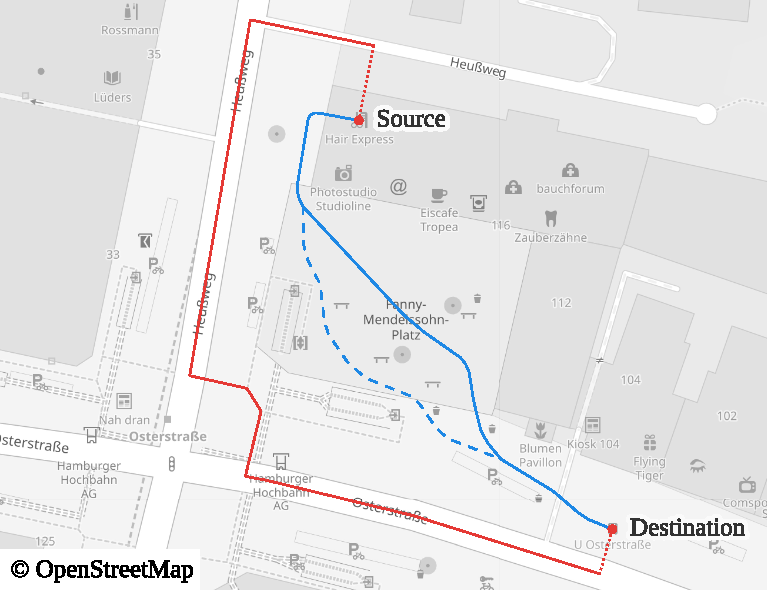
\includegraphics[width=\textwidth]{images/qgis-routing-osterstrasse-expected-vs-routing}
						\end{figcenter}
						\caption{The graph-based routing result (red) and the expected route (blue) a human would probably take. The red dotted parts are direct connections to the closest point on an edge.}
						\label{fig:eval-osterstrasse-route-expected}
					\end{subfigure}
				\end{minipage}
				\hfill
				\begin{minipage}[t]{.48\textwidth}
					\begin{subfigure}[t]{\linewidth}
						\begin{figcenter}
							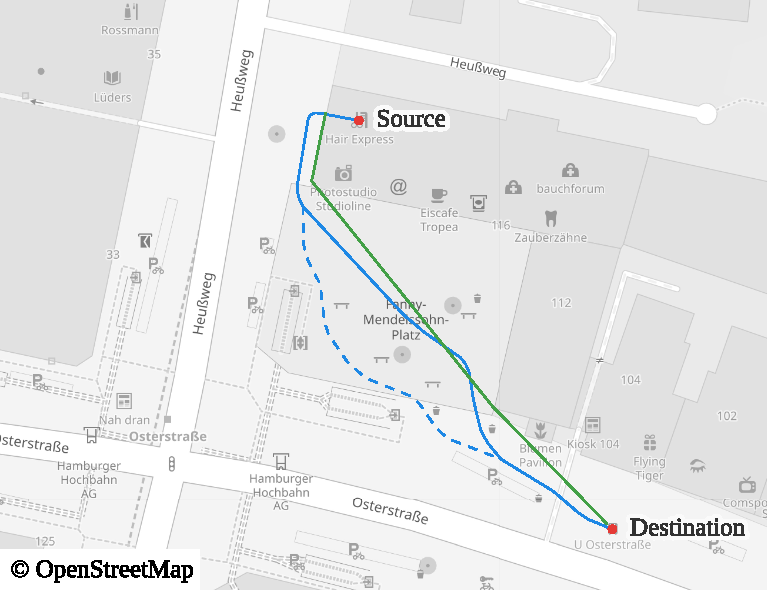
\includegraphics[width=\textwidth]{images/qgis-routing-osterstrasse-expected-vs-actual}
						\end{figcenter}
						\caption{The result of the hybrid routing algorithm (green) and the expected route (blue).}
						\label{fig:eval-osterstrasse-actual-expected}
					\end{subfigure}
				\end{minipage}
				\caption{Comparison of a graph-based route (determined on \href{https://www.openstreetmap.org/directions?engine=fossgis\_osrm\_foot\&route=53.57657\%2C9.95210\%3B53.57601\%2C9.95268\#map=19/53.57632/9.95218}{osm.org}) with the hybrid routing algorithm and the expected result (blue). The dashed part of the expected result is an equally good alternative route. The difficulty of this scenario is the traveral of the square \enquote{Fanny-Mendelssohn Platz}.}
				\label{fig:eval-osterstrasse}
			\end{figure}
			
			% Interesting passages from the city dataset
			Next to the above example and comparison to graph-based routing, an analysis of the routes determined within the 1km\textsuperscript{2} \enquote{OSM city} dataset yields some noteworthy findings.
			
			First, the quality of a route significantly decreases with missing or wrong data as visible in \Cref{fig:eval-city-usefulness-b} and \ref{fig:eval-city-usefulness-c}.
			The passages marked in red in these images are often shortcuts via private property.
			Those areas, however, are usually filled with obstacles such as fences, walls or different kinds of vegetation.
			As described in \Cref{subsubsec:data-not-in-osm}, private areas in OSM often contain very few to no details.
			
			Second, within densely built-up areas, larger open spaces are rare and the combination of roads and buildings form corrdidors in which routes tend to lie.
			When and how often the route determined by the hybrid routing algorithm follows a road depends on the weighting function.
			
			Third, large roads create instances of the aforementioned rare but wide obstacle-free areas, which, however, might result in unrealistic road crossings.
			Such situation can be seen in \Cref{fig:eval-city-road-crossing} with crossings over a six-lane road, which would be dangerous and unrealistic for real-world pedestrians.
			
			Forth, the weight function has a huge impact on the route quality.
			It specifies for example how strongly roads should be preferred, which is illustrated in \Cref{fig:eval-city-weights} with the same route using different weights for road edges.
			Adjusting and definiting fine-grained weight functions may help to imporove the routing behavior in some of the above mentioned situations.
			
			\begin{figure}[h!]
				\begin{minipage}[t]{.48\textwidth}
					\begin{subfigure}[t]{\linewidth}
						\begin{figcenter}
							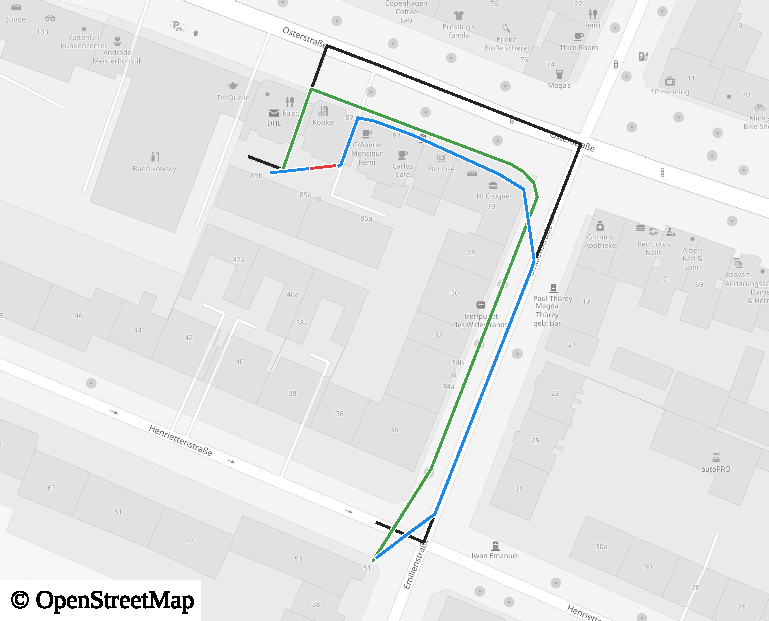
\includegraphics[width=\textwidth]{images/qgis-routing-city-routing-1}
						\end{figcenter}
						\caption{Simple route with only one small passage of missing data.}
						\label{fig:eval-city-usefulness-1}
					\end{subfigure}
				\end{minipage}
				\hfill
				\begin{minipage}[t]{.48\textwidth}
					\begin{subfigure}[t]{\linewidth}
						\begin{figcenter}
							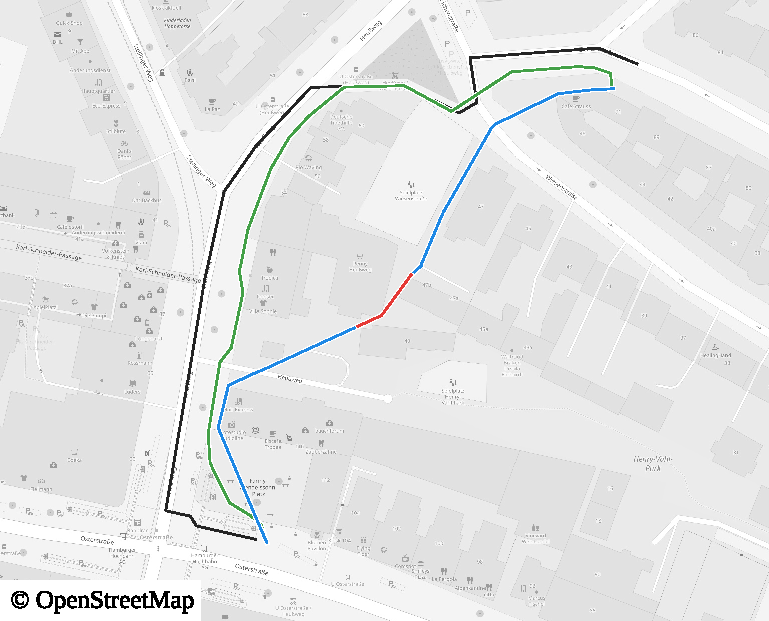
\includegraphics[width=\textwidth]{images/qgis-routing-city-routing-3}
						\end{figcenter}
						\caption{Missing obstacles (in this case walls and fences between buildings) might lead to non-realistic routes.}
						\label{fig:eval-city-usefulness-b}
					\end{subfigure}
				\end{minipage}
				\\
				\begin{minipage}[t]{.48\textwidth}
					\begin{subfigure}[t]{\linewidth}
						\begin{figcenter}
							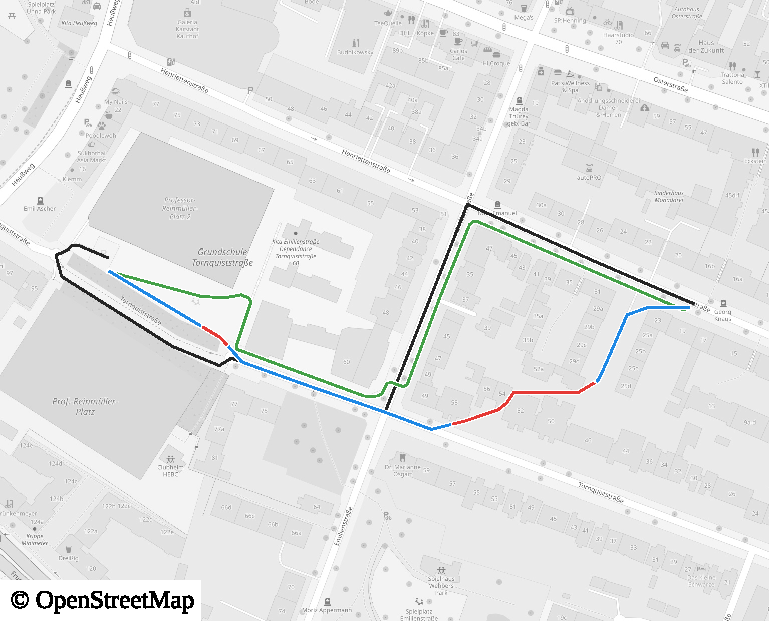
\includegraphics[width=\textwidth]{images/qgis-routing-city-routing-6}
						\end{figcenter}
						\caption{Missing walls, fences and hedges on private property are a common type of missing obstacles.}
						\label{fig:eval-city-usefulness-c}
					\end{subfigure}
				\end{minipage}
				\hfill
				\begin{minipage}[t]{.48\textwidth}
					\begin{subfigure}[t]{\linewidth}
						\begin{figcenter}
							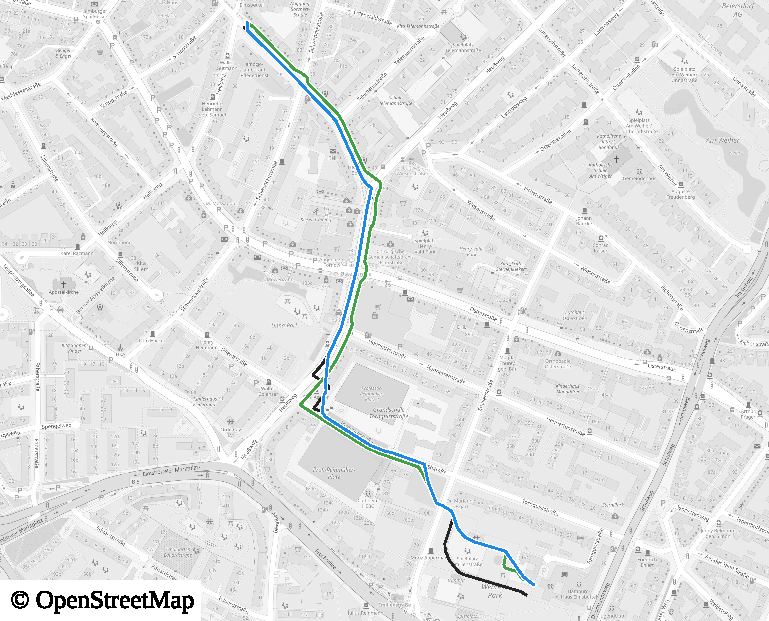
\includegraphics[width=\textwidth]{images/qgis-routing-city-routing-18}
						\end{figcenter}
						\caption{Cities with closed rows of buildings do not provide many degrees of freedom, which results in similar or even equal routes, regardles of the algorithm.}
						\label{fig:eval-city-usefulness-d}
					\end{subfigure}
				\end{minipage}
				\caption{Comparison of realistic routes (green), graph-based routing results (black) and hybrid routing algorithm results (blue) using the 1km\textsuperscript{2} \enquote{OSM city} dataset. Passages with missing or faulty data are marked in red, which are the main cause of the deviations to the expected route.}
				\label{fig:eval-city-usefulness}
				\begin{minipage}[t]{.48\textwidth}
					\begin{figcenter}
						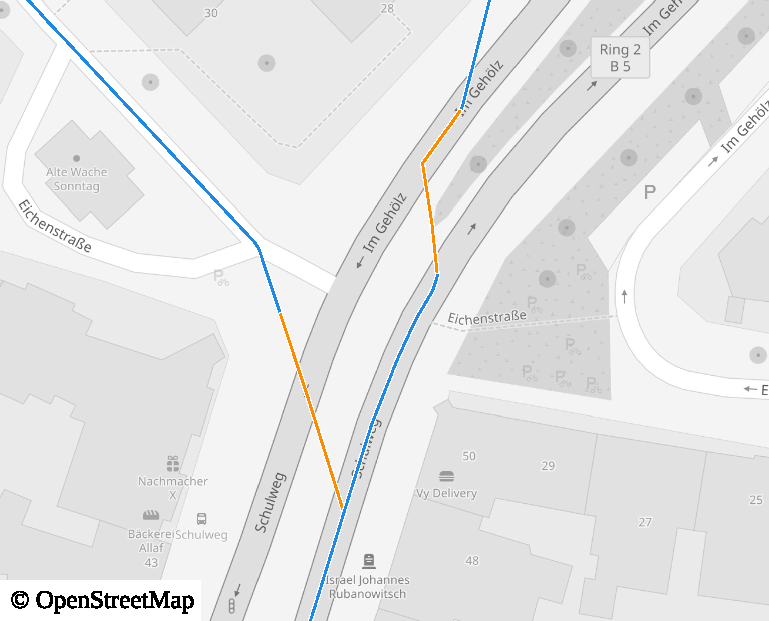
\includegraphics[width=\textwidth]{images/qgis-routing-city-roads}
					\end{figcenter}
					\caption{Two unrealistic road crossings (yellow) across a six-lane road.}
					\label{fig:eval-city-road-crossing}
				\end{minipage}
				\hfill
				\begin{minipage}[t]{.48\textwidth}
					\begin{figcenter}
						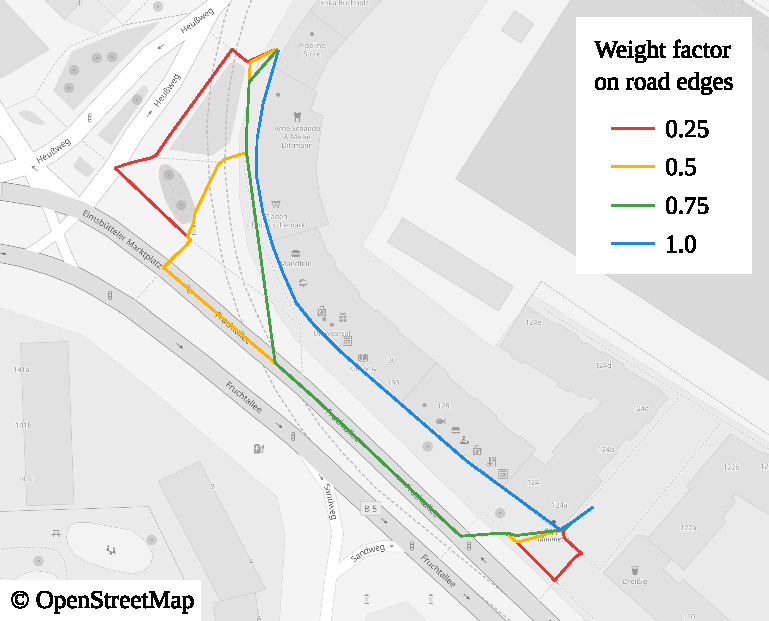
\includegraphics[width=\textwidth]{images/qgis-routing-city-weights}
					\end{figcenter}
					\caption{Influence of weight factors. Lower value result in a stronger preference for roads.}
					\label{fig:eval-city-weights}
				\end{minipage}
			\end{figure}
			
			% Interesting passages from the rural dataset
			In the \enquote{OSM city} datasets with only smaller open areas, graph-based routes and routes determined by the hybrid routing algorithm were often similar and some parts even identical.
			Datasets with larger open areas and irregular distributed obstacles, as in the \enquote{OSM rural} datasets, can greatly benefit from the hybrid routing algorithm.
			
			Figures \Cref{fig:eval-rural-routing-6} and \ref{fig:eval-rural-graph-based-comparison} give some examples on routes in a rural area with large open spaces.
			Two findings can be inferred from the analysis of the rural routing results.
			
			First, the difference between graph-based routes and routes from the hybrid routing algorithm is significantly larger.
			In fact, routes might not share any location and graph-based routes tend to be significantly longer.
			This can be seen in \Cref{fig:eval-rural-graph-based-comparison-6} with a graph-based route of 1.73km while the expected result is only 0.67km long.
			\Cref{fig:eval-rural-graph-based-comparison-17} shows a similar behavior even though the difference in distance is smaller because the graph-based, expected and actual route share common parts.
			
			Second, the accuracy and therefore the usefulness for real-world applications (such as navigation apps) heavily relies on the amount of details in the dataset.
			\Cref{fig:eval-rural-routing-6-osm} illustrates the problem of missing data, which are in this case missing ditches within the farmland.
			The determined route has a length of 365m while the shortest possible route (determined using aerial imagery as seen in \Cref{fig:eval-rural-routing-6-aerial}) is 677m long.
			
			\begin{figure}[h!]
				\begin{minipage}[t]{.48\textwidth}
					\begin{subfigure}[t]{\linewidth}
						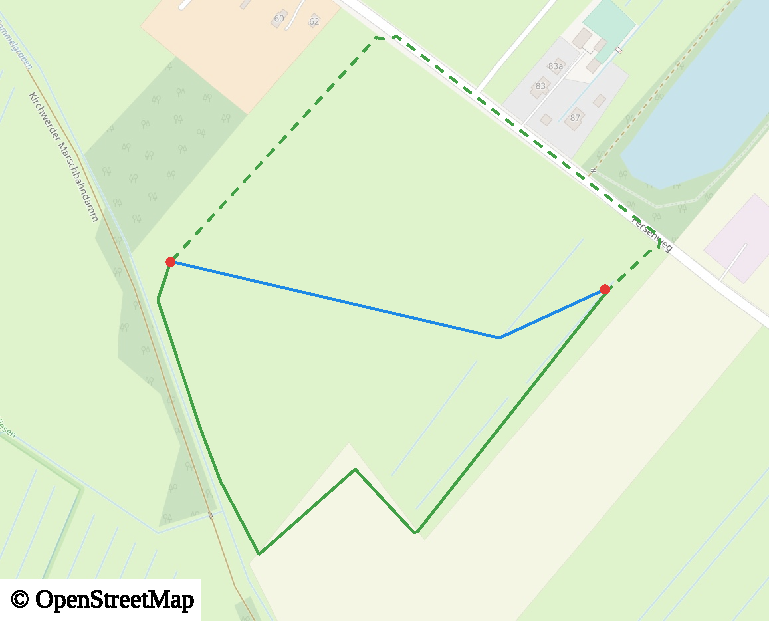
\includegraphics[width=\textwidth]{images/qgis-routing-rural-routing-6-osm}
						\caption{The expected route differs significantly from the actual route taken by the agent. The dashed line is an alternative route under the assumption, that the farmland is reachable from the upper road.}
						\label{fig:eval-rural-routing-6-osm}
					\end{subfigure}
				\end{minipage}
				\hfill
				\begin{minipage}[t]{.48\textwidth}
					\begin{subfigure}[t]{\linewidth}
						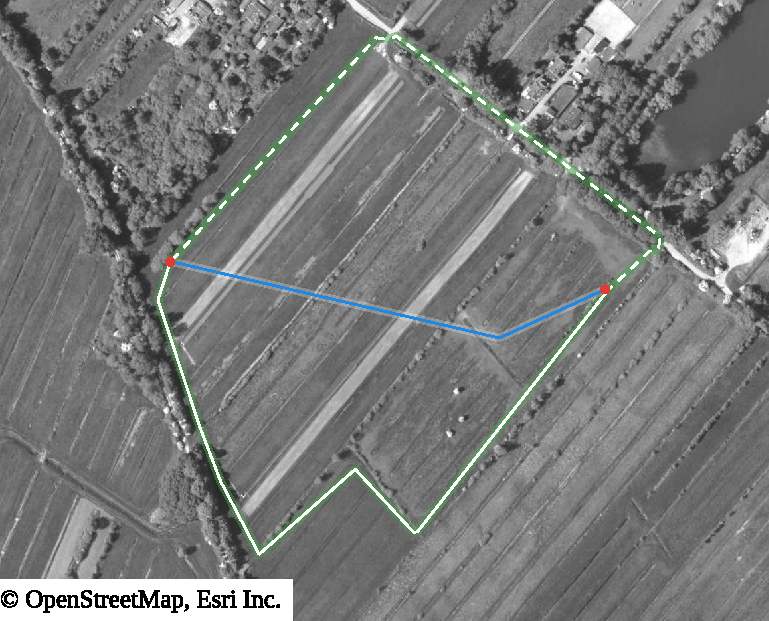
\includegraphics[width=\textwidth]{images/qgis-routing-rural-routing-6-aerial}
						\caption{Aerial imagery shows the amount of missing data, which in this case are numerous missing ditches in the arable land.}
						\label{fig:eval-rural-routing-6-aerial}
					\end{subfigure}
				\end{minipage}
				\caption{Routing on farmland illustrating the importance of correct data in the routing result showing the expected route (green) and actual path determined by the hybrid routing algorithm (green).}
				\label{fig:eval-rural-routing-6}
			\end{figure}
			
			\begin{figure}[h!]
				\begin{minipage}[t]{.48\textwidth}
					\begin{subfigure}[t]{\linewidth}
						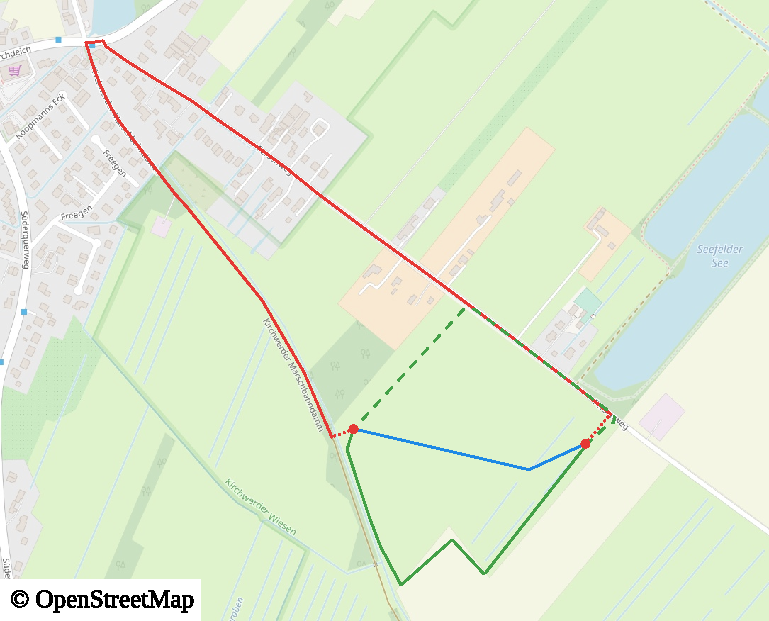
\includegraphics[width=\textwidth]{images/qgis-routing-rural-routing-6-graph-based}
						\caption{Same waypoints from \Cref{fig:eval-rural-routing-6} with the additional result of a graph-based routing request creating a 2.6 times longer path.}
						\label{fig:eval-rural-graph-based-comparison-6}
					\end{subfigure}
				\end{minipage}
				\hfill
				\begin{minipage}[t]{.48\textwidth}
					\begin{subfigure}[t]{\linewidth}
						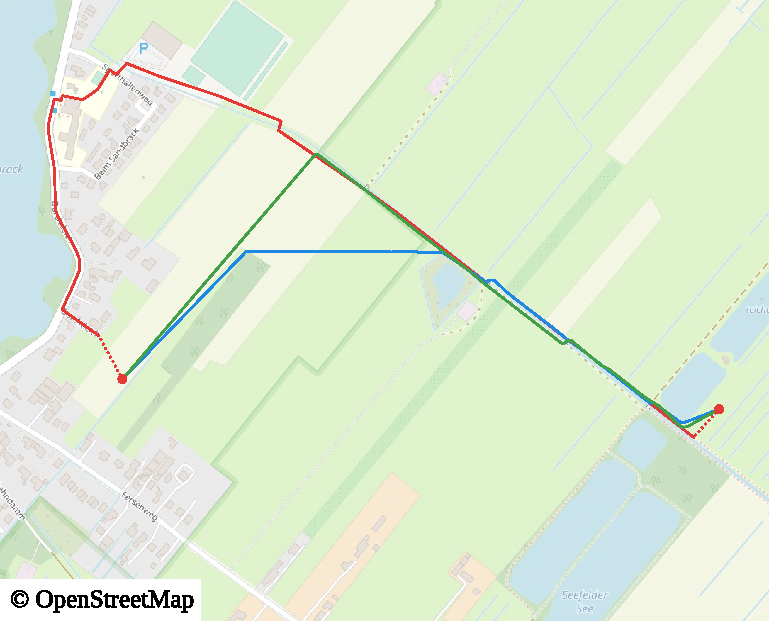
\includegraphics[width=\textwidth]{images/qgis-routing-rural-routing-17-graph-based}
						\caption{Example of detours created by a graph-based routing algorithm even though the first part of the result is equal to the one of the hybrid routing algorithm. The shortcut of the actual result (horizontal part of the blue route) is a result of missing obstacles similar to the situation visible in \Cref{fig:eval-rural-routing-6-aerial}.}
						\label{fig:eval-rural-graph-based-comparison-17}
					\end{subfigure}
				\end{minipage}
				\caption{Comparison of graph-based routing results (red) with the expected route (green) and actual results (blue) of the hybrid routing algorithm.}
				\label{fig:eval-rural-graph-based-comparison}
			\end{figure}
		
		\subsubsection{Mathematical route quality analysis}
			% Determine ratio of route lengths
			% Determine Frechet distance